\documentclass[twoside]{book}

% Packages required by doxygen
\usepackage{fixltx2e}
\usepackage{calc}
\usepackage{doxygen}
\usepackage[export]{adjustbox} % also loads graphicx
\usepackage{graphicx}
\usepackage[utf8]{inputenc}
\usepackage{makeidx}
\usepackage{multicol}
\usepackage{multirow}
\PassOptionsToPackage{warn}{textcomp}
\usepackage{textcomp}
\usepackage[nointegrals]{wasysym}
\usepackage[table]{xcolor}

% Font selection
\usepackage[T1]{fontenc}
\usepackage[scaled=.90]{helvet}
\usepackage{courier}
\usepackage{amssymb}
\usepackage{sectsty}
\renewcommand{\familydefault}{\sfdefault}
\allsectionsfont{%
  \fontseries{bc}\selectfont%
  \color{darkgray}%
}
\renewcommand{\DoxyLabelFont}{%
  \fontseries{bc}\selectfont%
  \color{darkgray}%
}
\newcommand{\+}{\discretionary{\mbox{\scriptsize$\hookleftarrow$}}{}{}}

% Page & text layout
\usepackage{geometry}
\geometry{%
  a4paper,%
  top=2.5cm,%
  bottom=2.5cm,%
  left=2.5cm,%
  right=2.5cm%
}
\tolerance=750
\hfuzz=15pt
\hbadness=750
\setlength{\emergencystretch}{15pt}
\setlength{\parindent}{0cm}
\setlength{\parskip}{3ex plus 2ex minus 2ex}
\makeatletter
\renewcommand{\paragraph}{%
  \@startsection{paragraph}{4}{0ex}{-1.0ex}{1.0ex}{%
    \normalfont\normalsize\bfseries\SS@parafont%
  }%
}
\renewcommand{\subparagraph}{%
  \@startsection{subparagraph}{5}{0ex}{-1.0ex}{1.0ex}{%
    \normalfont\normalsize\bfseries\SS@subparafont%
  }%
}
\makeatother

% Headers & footers
\usepackage{fancyhdr}
\pagestyle{fancyplain}
\fancyhead[LE]{\fancyplain{}{\bfseries\thepage}}
\fancyhead[CE]{\fancyplain{}{}}
\fancyhead[RE]{\fancyplain{}{\bfseries\leftmark}}
\fancyhead[LO]{\fancyplain{}{\bfseries\rightmark}}
\fancyhead[CO]{\fancyplain{}{}}
\fancyhead[RO]{\fancyplain{}{\bfseries\thepage}}
\fancyfoot[LE]{\fancyplain{}{}}
\fancyfoot[CE]{\fancyplain{}{}}
\fancyfoot[RE]{\fancyplain{}{\bfseries\scriptsize Generated by Doxygen }}
\fancyfoot[LO]{\fancyplain{}{\bfseries\scriptsize Generated by Doxygen }}
\fancyfoot[CO]{\fancyplain{}{}}
\fancyfoot[RO]{\fancyplain{}{}}
\renewcommand{\footrulewidth}{0.4pt}
\renewcommand{\chaptermark}[1]{%
  \markboth{#1}{}%
}
\renewcommand{\sectionmark}[1]{%
  \markright{\thesection\ #1}%
}

% Indices & bibliography
\usepackage{natbib}
\usepackage[titles]{tocloft}
\setcounter{tocdepth}{3}
\setcounter{secnumdepth}{5}
\makeindex

% Hyperlinks (required, but should be loaded last)
\usepackage{ifpdf}
\ifpdf
  \usepackage[pdftex,pagebackref=true]{hyperref}
\else
  \usepackage[ps2pdf,pagebackref=true]{hyperref}
\fi
\hypersetup{%
  colorlinks=true,%
  linkcolor=blue,%
  citecolor=blue,%
  unicode%
}

% Custom commands
\newcommand{\clearemptydoublepage}{%
  \newpage{\pagestyle{empty}\cleardoublepage}%
}

\usepackage{caption}
\captionsetup{labelsep=space,justification=centering,font={bf},singlelinecheck=off,skip=4pt,position=top}

%===== C O N T E N T S =====

\begin{document}

% Titlepage & ToC
\hypersetup{pageanchor=false,
             bookmarksnumbered=true,
             pdfencoding=unicode
            }
\pagenumbering{alph}
\begin{titlepage}
\vspace*{7cm}
\begin{center}%
{\Large Plotty\+Towers }\\
\vspace*{1cm}
{\large Generated by Doxygen 1.8.13}\\
\end{center}
\end{titlepage}
\clearemptydoublepage
\pagenumbering{roman}
\tableofcontents
\clearemptydoublepage
\pagenumbering{arabic}
\hypersetup{pageanchor=true}

%--- Begin generated contents ---
\chapter{Namespace Index}
\section{Packages}
Here are the packages with brief descriptions (if available)\+:\begin{DoxyCompactList}
\item\contentsline{section}{\hyperlink{namespaceenemies}{enemies} }{\pageref{namespaceenemies}}{}
\item\contentsline{section}{\hyperlink{namespaceevents}{events} }{\pageref{namespaceevents}}{}
\item\contentsline{section}{\hyperlink{namespacehelpz}{helpz} }{\pageref{namespacehelpz}}{}
\item\contentsline{section}{\hyperlink{namespaceinputs}{inputs} }{\pageref{namespaceinputs}}{}
\item\contentsline{section}{\hyperlink{namespacemanagers}{managers} }{\pageref{namespacemanagers}}{}
\item\contentsline{section}{\hyperlink{namespaceobjects}{objects} }{\pageref{namespaceobjects}}{}
\item\contentsline{section}{\hyperlink{namespaceprogetto}{progetto} }{\pageref{namespaceprogetto}}{}
\item\contentsline{section}{\hyperlink{namespacescenes}{scenes} }{\pageref{namespacescenes}}{}
\item\contentsline{section}{\hyperlink{namespacetowers}{towers} }{\pageref{namespacetowers}}{}
\item\contentsline{section}{\hyperlink{namespaceui}{ui} }{\pageref{namespaceui}}{}
\end{DoxyCompactList}

\chapter{Hierarchical Index}
\section{Class Hierarchy}
This inheritance list is sorted roughly, but not completely, alphabetically\+:\begin{DoxyCompactList}
\item \contentsline{section}{Attack\+Animation}{\pageref{classtowers_1_1_attack_animation}}{}
\item \contentsline{section}{Bar}{\pageref{classui_1_1_bar}}{}
\begin{DoxyCompactList}
\item \contentsline{section}{Action\+Bar}{\pageref{classui_1_1_action_bar}}{}
\item \contentsline{section}{Tool\+Bar}{\pageref{classui_1_1_tool_bar}}{}
\end{DoxyCompactList}
\item \contentsline{section}{Constants}{\pageref{classhelpz_1_1_constants}}{}
\item \contentsline{section}{Constants.\+Direction}{\pageref{classhelpz_1_1_constants_1_1_direction}}{}
\item \contentsline{section}{Enemy}{\pageref{classenemies_1_1_enemy}}{}
\item \contentsline{section}{Constants.\+Enemy}{\pageref{classhelpz_1_1_constants_1_1_enemy}}{}
\item \contentsline{section}{Enemy\+Manager}{\pageref{classmanagers_1_1_enemy_manager}}{}
\item \contentsline{section}{Game\+Scene}{\pageref{classscenes_1_1_game_scene}}{}
\begin{DoxyCompactList}
\item \contentsline{section}{Editing}{\pageref{classscenes_1_1_editing}}{}
\item \contentsline{section}{Level1}{\pageref{classscenes_1_1_level1}}{}
\item \contentsline{section}{Level2}{\pageref{classscenes_1_1_level2}}{}
\item \contentsline{section}{Level3}{\pageref{classscenes_1_1_level3}}{}
\item \contentsline{section}{Level4}{\pageref{classscenes_1_1_level4}}{}
\item \contentsline{section}{Menu}{\pageref{classscenes_1_1_menu}}{}
\item \contentsline{section}{Playing}{\pageref{classscenes_1_1_playing}}{}
\end{DoxyCompactList}
\item \contentsline{section}{Game\+States}{\pageref{enumprogetto_1_1_game_states}}{}
\item \contentsline{section}{Img\+Fix}{\pageref{classhelpz_1_1_img_fix}}{}
\item \contentsline{section}{Level\+Menu}{\pageref{classui_1_1_level_menu}}{}
\item \contentsline{section}{Load\+Save}{\pageref{classhelpz_1_1_load_save}}{}
\item \contentsline{section}{My\+Button}{\pageref{classui_1_1_my_button}}{}
\item \contentsline{section}{Pause\+Button}{\pageref{classui_1_1_pause_button}}{}
\begin{DoxyCompactList}
\item \contentsline{section}{Sound\+Button}{\pageref{classui_1_1_sound_button}}{}
\item \contentsline{section}{Ush\+Button}{\pageref{classui_1_1_ush_button}}{}
\end{DoxyCompactList}
\item \contentsline{section}{Pause\+Overlay}{\pageref{classui_1_1_pause_overlay}}{}
\item \contentsline{section}{Projectile}{\pageref{classobjects_1_1_projectile}}{}
\item \contentsline{section}{Projectile\+Manager}{\pageref{classmanagers_1_1_projectile_manager}}{}
\item \contentsline{section}{Constants.\+Projectiles}{\pageref{classhelpz_1_1_constants_1_1_projectiles}}{}
\item \contentsline{section}{Render}{\pageref{classprogetto_1_1_render}}{}
\item Runnable\begin{DoxyCompactList}
\item \contentsline{section}{Game}{\pageref{classprogetto_1_1_game}}{}
\end{DoxyCompactList}
\item \contentsline{section}{Scene\+Methods}{\pageref{interfacescenes_1_1_scene_methods}}{}
\begin{DoxyCompactList}
\item \contentsline{section}{Editing}{\pageref{classscenes_1_1_editing}}{}
\item \contentsline{section}{Level1}{\pageref{classscenes_1_1_level1}}{}
\item \contentsline{section}{Level2}{\pageref{classscenes_1_1_level2}}{}
\item \contentsline{section}{Level3}{\pageref{classscenes_1_1_level3}}{}
\item \contentsline{section}{Level4}{\pageref{classscenes_1_1_level4}}{}
\item \contentsline{section}{Menu}{\pageref{classscenes_1_1_menu}}{}
\item \contentsline{section}{Playing}{\pageref{classscenes_1_1_playing}}{}
\end{DoxyCompactList}
\item \contentsline{section}{Sound}{\pageref{classprogetto_1_1_sound}}{}
\item Thread\begin{DoxyCompactList}
\item \contentsline{section}{Thread\+Update}{\pageref{classprogetto_1_1_thread_update}}{}
\end{DoxyCompactList}
\item \contentsline{section}{Tile}{\pageref{classobjects_1_1_tile}}{}
\item \contentsline{section}{Tile\+Manager}{\pageref{classmanagers_1_1_tile_manager}}{}
\item \contentsline{section}{Constants.\+Tiles}{\pageref{classhelpz_1_1_constants_1_1_tiles}}{}
\item \contentsline{section}{Tower}{\pageref{classtowers_1_1_tower}}{}
\item \contentsline{section}{Tower\+Manager}{\pageref{classmanagers_1_1_tower_manager}}{}
\item \contentsline{section}{Constants.\+Towers}{\pageref{classhelpz_1_1_constants_1_1_towers}}{}
\item \contentsline{section}{Utilz}{\pageref{classhelpz_1_1_utilz}}{}
\item \contentsline{section}{Wave}{\pageref{classevents_1_1_wave}}{}
\item \contentsline{section}{Wave\+Manager}{\pageref{classmanagers_1_1_wave_manager}}{}
\item J\+Frame\begin{DoxyCompactList}
\item \contentsline{section}{Game}{\pageref{classprogetto_1_1_game}}{}
\end{DoxyCompactList}
\item J\+Panel\begin{DoxyCompactList}
\item \contentsline{section}{Game\+Screen}{\pageref{classprogetto_1_1_game_screen}}{}
\end{DoxyCompactList}
\item Key\+Listener\begin{DoxyCompactList}
\item \contentsline{section}{Keyboard\+Listener}{\pageref{classinputs_1_1_keyboard_listener}}{}
\end{DoxyCompactList}
\item Mouse\+Listener\begin{DoxyCompactList}
\item \contentsline{section}{My\+Mouse\+Listener}{\pageref{classinputs_1_1_my_mouse_listener}}{}
\end{DoxyCompactList}
\item Mouse\+Motion\+Listener\begin{DoxyCompactList}
\item \contentsline{section}{My\+Mouse\+Listener}{\pageref{classinputs_1_1_my_mouse_listener}}{}
\end{DoxyCompactList}
\end{DoxyCompactList}

\chapter{Class Index}
\section{Class List}
Here are the classes, structs, unions and interfaces with brief descriptions\+:\begin{DoxyCompactList}
\item\contentsline{section}{\hyperlink{classui_1_1_action_bar}{Action\+Bar} \\*Classe figlia della classe \char`\"{}\+Bar\char`\"{} per gestire la barra presente nei livelli }{\pageref{classui_1_1_action_bar}}{}
\item\contentsline{section}{\hyperlink{classtowers_1_1_attack_animation}{Attack\+Animation} \\*Gestisce le varie animazioni per ogni proiettile }{\pageref{classtowers_1_1_attack_animation}}{}
\item\contentsline{section}{\hyperlink{classui_1_1_bar}{Bar} \\*Classe padre delle altre barre }{\pageref{classui_1_1_bar}}{}
\item\contentsline{section}{\hyperlink{classhelpz_1_1_constants}{Constants} \\*Gestisce le costanti }{\pageref{classhelpz_1_1_constants}}{}
\item\contentsline{section}{\hyperlink{classhelpz_1_1_constants_1_1_direction}{Constants.\+Direction} }{\pageref{classhelpz_1_1_constants_1_1_direction}}{}
\item\contentsline{section}{\hyperlink{classscenes_1_1_editing}{Editing} \\*Gestice le mappe, le modifiche e i salvataggi di esse }{\pageref{classscenes_1_1_editing}}{}
\item\contentsline{section}{\hyperlink{classenemies_1_1_enemy}{Enemy} \\*Gestisce i nemici e i loro attributi }{\pageref{classenemies_1_1_enemy}}{}
\item\contentsline{section}{\hyperlink{classhelpz_1_1_constants_1_1_enemy}{Constants.\+Enemy} }{\pageref{classhelpz_1_1_constants_1_1_enemy}}{}
\item\contentsline{section}{\hyperlink{classmanagers_1_1_enemy_manager}{Enemy\+Manager} \\*Classe per gestire il movimento, la vita e le animazioni dei nemici }{\pageref{classmanagers_1_1_enemy_manager}}{}
\item\contentsline{section}{\hyperlink{classprogetto_1_1_game}{Game} \\*J\+Frame main gestisce la schermata di gioco }{\pageref{classprogetto_1_1_game}}{}
\item\contentsline{section}{\hyperlink{classscenes_1_1_game_scene}{Game\+Scene} \\*Setter e getter del game per \char`\"{}collegare\char`\"{} le scene con i metodi del game }{\pageref{classscenes_1_1_game_scene}}{}
\item\contentsline{section}{\hyperlink{classprogetto_1_1_game_screen}{Game\+Screen} \\*J\+Frame J\+Panel gestisce le print e i comandi input }{\pageref{classprogetto_1_1_game_screen}}{}
\item\contentsline{section}{\hyperlink{enumprogetto_1_1_game_states}{Game\+States} }{\pageref{enumprogetto_1_1_game_states}}{}
\item\contentsline{section}{\hyperlink{classhelpz_1_1_img_fix}{Img\+Fix} \\*Gestisce gli aggiustamenti delle immagini }{\pageref{classhelpz_1_1_img_fix}}{}
\item\contentsline{section}{\hyperlink{classinputs_1_1_keyboard_listener}{Keyboard\+Listener} }{\pageref{classinputs_1_1_keyboard_listener}}{}
\item\contentsline{section}{\hyperlink{classscenes_1_1_level1}{Level1} \\*Classe che gestisce tutti gli elementi e i metodi del \hyperlink{classscenes_1_1_level1}{Level1} }{\pageref{classscenes_1_1_level1}}{}
\item\contentsline{section}{\hyperlink{classscenes_1_1_level2}{Level2} \\*Classe che gestisce tutti gli elementi e i metodi del \hyperlink{classscenes_1_1_level2}{Level2} }{\pageref{classscenes_1_1_level2}}{}
\item\contentsline{section}{\hyperlink{classscenes_1_1_level3}{Level3} \\*Classe che gestisce tutti gli elementi e i metodi del \hyperlink{classscenes_1_1_level4}{Level4} }{\pageref{classscenes_1_1_level3}}{}
\item\contentsline{section}{\hyperlink{classscenes_1_1_level4}{Level4} \\*Classe che gestisce tutti gli elementi e i metodi del \hyperlink{classscenes_1_1_level4}{Level4} }{\pageref{classscenes_1_1_level4}}{}
\item\contentsline{section}{\hyperlink{classui_1_1_level_menu}{Level\+Menu} \\*Classe per la gestione degli eventi del mouse e dei bottoni presenti nel menu dei livelli }{\pageref{classui_1_1_level_menu}}{}
\item\contentsline{section}{\hyperlink{classhelpz_1_1_load_save}{Load\+Save} \\*Carica e salva immagini e mappe }{\pageref{classhelpz_1_1_load_save}}{}
\item\contentsline{section}{\hyperlink{classscenes_1_1_menu}{Menu} \\*Gestice il menu\+: sfondo, bottoni }{\pageref{classscenes_1_1_menu}}{}
\item\contentsline{section}{\hyperlink{classui_1_1_my_button}{My\+Button} \\*Gestisce i diversi tipi di bottone con i diversi costruttori ed i diversi modi di stamparli }{\pageref{classui_1_1_my_button}}{}
\item\contentsline{section}{\hyperlink{classinputs_1_1_my_mouse_listener}{My\+Mouse\+Listener} }{\pageref{classinputs_1_1_my_mouse_listener}}{}
\item\contentsline{section}{\hyperlink{classui_1_1_pause_button}{Pause\+Button} \\*Gestisce il bottone di pausa }{\pageref{classui_1_1_pause_button}}{}
\item\contentsline{section}{\hyperlink{classui_1_1_pause_overlay}{Pause\+Overlay} \\*Gestisce l\textquotesingle{}overlay di gioco in pausa }{\pageref{classui_1_1_pause_overlay}}{}
\item\contentsline{section}{\hyperlink{classscenes_1_1_playing}{Playing} \\*Gestice il menu dei livelli\+: sfondo, bottoni }{\pageref{classscenes_1_1_playing}}{}
\item\contentsline{section}{\hyperlink{classobjects_1_1_projectile}{Projectile} \\*Gestisce gli oggetti proiettile e tutti i loro attributi }{\pageref{classobjects_1_1_projectile}}{}
\item\contentsline{section}{\hyperlink{classmanagers_1_1_projectile_manager}{Projectile\+Manager} \\*Classe per gestire il movimento, l\textquotesingle{}inclinazione, la posizione dei proiettili interazioni dei proiettili coi nemici }{\pageref{classmanagers_1_1_projectile_manager}}{}
\item\contentsline{section}{\hyperlink{classhelpz_1_1_constants_1_1_projectiles}{Constants.\+Projectiles} }{\pageref{classhelpz_1_1_constants_1_1_projectiles}}{}
\item\contentsline{section}{\hyperlink{classprogetto_1_1_render}{Render} \\*Gestione rendering del gioco }{\pageref{classprogetto_1_1_render}}{}
\item\contentsline{section}{\hyperlink{interfacescenes_1_1_scene_methods}{Scene\+Methods} }{\pageref{interfacescenes_1_1_scene_methods}}{}
\item\contentsline{section}{\hyperlink{classprogetto_1_1_sound}{Sound} \\*Classe per la gestione completa dei suoni livello per livello }{\pageref{classprogetto_1_1_sound}}{}
\item\contentsline{section}{\hyperlink{classui_1_1_sound_button}{Sound\+Button} \\*Gestice il bottone che smuta e muta la musica }{\pageref{classui_1_1_sound_button}}{}
\item\contentsline{section}{\hyperlink{classprogetto_1_1_thread_update}{Thread\+Update} \\*Serve per gestire i vari metodi di update delle schermate richiamando solo l\textquotesingle{}update corrispondente ad esse }{\pageref{classprogetto_1_1_thread_update}}{}
\item\contentsline{section}{\hyperlink{classobjects_1_1_tile}{Tile} \\*Gestisce gli oggetti tile e i loro attributi }{\pageref{classobjects_1_1_tile}}{}
\item\contentsline{section}{\hyperlink{classmanagers_1_1_tile_manager}{Tile\+Manager} \\*Classe per gestire i tile della mappa }{\pageref{classmanagers_1_1_tile_manager}}{}
\item\contentsline{section}{\hyperlink{classhelpz_1_1_constants_1_1_tiles}{Constants.\+Tiles} }{\pageref{classhelpz_1_1_constants_1_1_tiles}}{}
\item\contentsline{section}{\hyperlink{classui_1_1_tool_bar}{Tool\+Bar} \\*Gestice la barra per modificare le mappe dei vari livelli e salvarle }{\pageref{classui_1_1_tool_bar}}{}
\item\contentsline{section}{\hyperlink{classtowers_1_1_tower}{Tower} \\*Gestisce gli oggetti delle torri }{\pageref{classtowers_1_1_tower}}{}
\item\contentsline{section}{\hyperlink{classmanagers_1_1_tower_manager}{Tower\+Manager} \\*Classe per gestire il numero, la rimozione, gli upgrade, la creazione, le animazioni e gli spari delle torri }{\pageref{classmanagers_1_1_tower_manager}}{}
\item\contentsline{section}{\hyperlink{classhelpz_1_1_constants_1_1_towers}{Constants.\+Towers} }{\pageref{classhelpz_1_1_constants_1_1_towers}}{}
\item\contentsline{section}{\hyperlink{classui_1_1_ush_button}{Ush\+Button} \\*Gestisce i bottoni adibiti all\textquotesingle{}resume, restart e quit presenti nella pause\+Overlay }{\pageref{classui_1_1_ush_button}}{}
\item\contentsline{section}{\hyperlink{classhelpz_1_1_utilz}{Utilz} \\*Contiene metodi utili al progetto }{\pageref{classhelpz_1_1_utilz}}{}
\item\contentsline{section}{\hyperlink{classevents_1_1_wave}{Wave} \\*Gestisce le ondate }{\pageref{classevents_1_1_wave}}{}
\item\contentsline{section}{\hyperlink{classmanagers_1_1_wave_manager}{Wave\+Manager} \\*Classe per gestire il numero di ondate, che nemici contengono, ogni quanto generano un nemico e dopo quanto parte un\textquotesingle{}altra ondata }{\pageref{classmanagers_1_1_wave_manager}}{}
\end{DoxyCompactList}

\chapter{File Index}
\section{File List}
Here is a list of all files with brief descriptions\+:\begin{DoxyCompactList}
\item\contentsline{section}{C\+:/\+Users/\+Utente/\+Documents/\+Git\+Hub/\+Plotty\+Towers/progetto/src/enemies/\hyperlink{_enemy_8java}{Enemy.\+java} }{\pageref{_enemy_8java}}{}
\item\contentsline{section}{C\+:/\+Users/\+Utente/\+Documents/\+Git\+Hub/\+Plotty\+Towers/progetto/src/events/\hyperlink{_wave_8java}{Wave.\+java} }{\pageref{_wave_8java}}{}
\item\contentsline{section}{C\+:/\+Users/\+Utente/\+Documents/\+Git\+Hub/\+Plotty\+Towers/progetto/src/helpz/\hyperlink{_constants_8java}{Constants.\+java} \\*Gestisce le costanti }{\pageref{_constants_8java}}{}
\item\contentsline{section}{C\+:/\+Users/\+Utente/\+Documents/\+Git\+Hub/\+Plotty\+Towers/progetto/src/helpz/\hyperlink{_img_fix_8java}{Img\+Fix.\+java} \\*Aggiusta le immagini }{\pageref{_img_fix_8java}}{}
\item\contentsline{section}{C\+:/\+Users/\+Utente/\+Documents/\+Git\+Hub/\+Plotty\+Towers/progetto/src/helpz/\hyperlink{_load_save_8java}{Load\+Save.\+java} \\*Carica e salva immagini e mappe }{\pageref{_load_save_8java}}{}
\item\contentsline{section}{C\+:/\+Users/\+Utente/\+Documents/\+Git\+Hub/\+Plotty\+Towers/progetto/src/helpz/\hyperlink{_utilz_8java}{Utilz.\+java} }{\pageref{_utilz_8java}}{}
\item\contentsline{section}{C\+:/\+Users/\+Utente/\+Documents/\+Git\+Hub/\+Plotty\+Towers/progetto/src/inputs/\hyperlink{_keyboard_listener_8java}{Keyboard\+Listener.\+java} }{\pageref{_keyboard_listener_8java}}{}
\item\contentsline{section}{C\+:/\+Users/\+Utente/\+Documents/\+Git\+Hub/\+Plotty\+Towers/progetto/src/inputs/\hyperlink{_my_mouse_listener_8java}{My\+Mouse\+Listener.\+java} }{\pageref{_my_mouse_listener_8java}}{}
\item\contentsline{section}{C\+:/\+Users/\+Utente/\+Documents/\+Git\+Hub/\+Plotty\+Towers/progetto/src/managers/\hyperlink{_enemy_manager_8java}{Enemy\+Manager.\+java} }{\pageref{_enemy_manager_8java}}{}
\item\contentsline{section}{C\+:/\+Users/\+Utente/\+Documents/\+Git\+Hub/\+Plotty\+Towers/progetto/src/managers/\hyperlink{_projectile_manager_8java}{Projectile\+Manager.\+java} }{\pageref{_projectile_manager_8java}}{}
\item\contentsline{section}{C\+:/\+Users/\+Utente/\+Documents/\+Git\+Hub/\+Plotty\+Towers/progetto/src/managers/\hyperlink{_tile_manager_8java}{Tile\+Manager.\+java} }{\pageref{_tile_manager_8java}}{}
\item\contentsline{section}{C\+:/\+Users/\+Utente/\+Documents/\+Git\+Hub/\+Plotty\+Towers/progetto/src/managers/\hyperlink{_tower_manager_8java}{Tower\+Manager.\+java} }{\pageref{_tower_manager_8java}}{}
\item\contentsline{section}{C\+:/\+Users/\+Utente/\+Documents/\+Git\+Hub/\+Plotty\+Towers/progetto/src/managers/\hyperlink{_wave_manager_8java}{Wave\+Manager.\+java} }{\pageref{_wave_manager_8java}}{}
\item\contentsline{section}{C\+:/\+Users/\+Utente/\+Documents/\+Git\+Hub/\+Plotty\+Towers/progetto/src/objects/\hyperlink{_projectile_8java}{Projectile.\+java} \\*Gestisce gli oggetti proiettile }{\pageref{_projectile_8java}}{}
\item\contentsline{section}{C\+:/\+Users/\+Utente/\+Documents/\+Git\+Hub/\+Plotty\+Towers/progetto/src/objects/\hyperlink{_tile_8java}{Tile.\+java} \\*Gestisce gli oggetti Tile }{\pageref{_tile_8java}}{}
\item\contentsline{section}{C\+:/\+Users/\+Utente/\+Documents/\+Git\+Hub/\+Plotty\+Towers/progetto/src/progetto/\hyperlink{_game_8java}{Game.\+java} \\*Il file main che gestisce tutto il progetto, contiene i vari thread e tutte le classi del progetto }{\pageref{_game_8java}}{}
\item\contentsline{section}{C\+:/\+Users/\+Utente/\+Documents/\+Git\+Hub/\+Plotty\+Towers/progetto/src/progetto/\hyperlink{_game_screen_8java}{Game\+Screen.\+java} \\*File della classe J\+Panel Game\+Screen che gestisce tutte le print che saranno eseguite nella schermata di gioco e gli imput da tastiera e mouse }{\pageref{_game_screen_8java}}{}
\item\contentsline{section}{C\+:/\+Users/\+Utente/\+Documents/\+Git\+Hub/\+Plotty\+Towers/progetto/src/progetto/\hyperlink{_game_states_8java}{Game\+States.\+java} \\*File d\textquotesingle{}enumerazione a scopo di semplificare la modifica della schermata visualizzata }{\pageref{_game_states_8java}}{}
\item\contentsline{section}{C\+:/\+Users/\+Utente/\+Documents/\+Git\+Hub/\+Plotty\+Towers/progetto/src/progetto/\hyperlink{_render_8java}{Render.\+java} \\*File che gestisce il richiamo del metodo render nella classe interessata }{\pageref{_render_8java}}{}
\item\contentsline{section}{C\+:/\+Users/\+Utente/\+Documents/\+Git\+Hub/\+Plotty\+Towers/progetto/src/progetto/\hyperlink{_sound_8java}{Sound.\+java} \\*Gestisce tutti i suoni }{\pageref{_sound_8java}}{}
\item\contentsline{section}{C\+:/\+Users/\+Utente/\+Documents/\+Git\+Hub/\+Plotty\+Towers/progetto/src/progetto/\hyperlink{_thread_update_8java}{Thread\+Update.\+java} \\*Gestisce il richiamo dei metodi per l\textquotesingle{}aggiornare il gioco }{\pageref{_thread_update_8java}}{}
\item\contentsline{section}{C\+:/\+Users/\+Utente/\+Documents/\+Git\+Hub/\+Plotty\+Towers/progetto/src/scenes/\hyperlink{_editing_8java}{Editing.\+java} \\*Gestisce la schermata di edit della mappa }{\pageref{_editing_8java}}{}
\item\contentsline{section}{C\+:/\+Users/\+Utente/\+Documents/\+Git\+Hub/\+Plotty\+Towers/progetto/src/scenes/\hyperlink{_game_scene_8java}{Game\+Scene.\+java} \\*File per intermediare fra le scene ed il game }{\pageref{_game_scene_8java}}{}
\item\contentsline{section}{C\+:/\+Users/\+Utente/\+Documents/\+Git\+Hub/\+Plotty\+Towers/progetto/src/scenes/\hyperlink{_level1_8java}{Level1.\+java} \\*File per gestire i nemici e il pathfinding }{\pageref{_level1_8java}}{}
\item\contentsline{section}{C\+:/\+Users/\+Utente/\+Documents/\+Git\+Hub/\+Plotty\+Towers/progetto/src/scenes/\hyperlink{_level2_8java}{Level2.\+java} \\*File per gestire tutto cio che è presente nel level2 }{\pageref{_level2_8java}}{}
\item\contentsline{section}{C\+:/\+Users/\+Utente/\+Documents/\+Git\+Hub/\+Plotty\+Towers/progetto/src/scenes/\hyperlink{_level3_8java}{Level3.\+java} \\*File per gestire tutto cio che è presente nel level3 }{\pageref{_level3_8java}}{}
\item\contentsline{section}{C\+:/\+Users/\+Utente/\+Documents/\+Git\+Hub/\+Plotty\+Towers/progetto/src/scenes/\hyperlink{_level4_8java}{Level4.\+java} \\*File per gestire tutto cio che è presente nel level4 }{\pageref{_level4_8java}}{}
\item\contentsline{section}{C\+:/\+Users/\+Utente/\+Documents/\+Git\+Hub/\+Plotty\+Towers/progetto/src/scenes/\hyperlink{_menu_8java}{Menu.\+java} }{\pageref{_menu_8java}}{}
\item\contentsline{section}{C\+:/\+Users/\+Utente/\+Documents/\+Git\+Hub/\+Plotty\+Towers/progetto/src/scenes/\hyperlink{_playing_8java}{Playing.\+java} \\*Gestisce la schermata del menu dei livelli }{\pageref{_playing_8java}}{}
\item\contentsline{section}{C\+:/\+Users/\+Utente/\+Documents/\+Git\+Hub/\+Plotty\+Towers/progetto/src/scenes/\hyperlink{_scene_methods_8java}{Scene\+Methods.\+java} }{\pageref{_scene_methods_8java}}{}
\item\contentsline{section}{C\+:/\+Users/\+Utente/\+Documents/\+Git\+Hub/\+Plotty\+Towers/progetto/src/towers/\hyperlink{_attack_animation_8java}{Attack\+Animation.\+java} \\*Gestisce le animazioni dei proiettili/attacchi }{\pageref{_attack_animation_8java}}{}
\item\contentsline{section}{C\+:/\+Users/\+Utente/\+Documents/\+Git\+Hub/\+Plotty\+Towers/progetto/src/towers/\hyperlink{_tower_8java}{Tower.\+java} }{\pageref{_tower_8java}}{}
\item\contentsline{section}{C\+:/\+Users/\+Utente/\+Documents/\+Git\+Hub/\+Plotty\+Towers/progetto/src/ui/\hyperlink{_action_bar_8java}{Action\+Bar.\+java} \\*Barra visualizzata nei livelli contenente le varie difese, con le loro info, e informazioni vita ondata ecc }{\pageref{_action_bar_8java}}{}
\item\contentsline{section}{C\+:/\+Users/\+Utente/\+Documents/\+Git\+Hub/\+Plotty\+Towers/progetto/src/ui/\hyperlink{_bar_8java}{Bar.\+java} \\*Barra per gestire le classi figlie con posizione (x, y) e dimensioni }{\pageref{_bar_8java}}{}
\item\contentsline{section}{C\+:/\+Users/\+Utente/\+Documents/\+Git\+Hub/\+Plotty\+Towers/progetto/src/ui/\hyperlink{_level_menu_8java}{Level\+Menu.\+java} \\*File per la gestione delle componenti grafiche presenti nella schermata del menu dei livelli }{\pageref{_level_menu_8java}}{}
\item\contentsline{section}{C\+:/\+Users/\+Utente/\+Documents/\+Git\+Hub/\+Plotty\+Towers/progetto/src/ui/\hyperlink{_my_button_8java}{My\+Button.\+java} \\*File per la gestione completa di ogni tipo di bottone }{\pageref{_my_button_8java}}{}
\item\contentsline{section}{C\+:/\+Users/\+Utente/\+Documents/\+Git\+Hub/\+Plotty\+Towers/progetto/src/ui/\hyperlink{_pause_button_8java}{Pause\+Button.\+java} \\*Bottone per mettere in pausa le schermate di gioco e aprire l\textquotesingle{}overlay\+Pause }{\pageref{_pause_button_8java}}{}
\item\contentsline{section}{C\+:/\+Users/\+Utente/\+Documents/\+Git\+Hub/\+Plotty\+Towers/progetto/src/ui/\hyperlink{_pause_overlay_8java}{Pause\+Overlay.\+java} \\*Overlay del gioco quando un livello viene messo in pausa }{\pageref{_pause_overlay_8java}}{}
\item\contentsline{section}{C\+:/\+Users/\+Utente/\+Documents/\+Git\+Hub/\+Plotty\+Towers/progetto/src/ui/\hyperlink{_sound_button_8java}{Sound\+Button.\+java} \\*Bottone per mutare e smutare la musica }{\pageref{_sound_button_8java}}{}
\item\contentsline{section}{C\+:/\+Users/\+Utente/\+Documents/\+Git\+Hub/\+Plotty\+Towers/progetto/src/ui/\hyperlink{_tool_bar_8java}{Tool\+Bar.\+java} \\*Barra per la modifica della mappa }{\pageref{_tool_bar_8java}}{}
\item\contentsline{section}{C\+:/\+Users/\+Utente/\+Documents/\+Git\+Hub/\+Plotty\+Towers/progetto/src/ui/\hyperlink{_ush_button_8java}{Ush\+Button.\+java} \\*Bottoni dell\textquotesingle{}pause\+Overlay per restartare, riprendere ed uscire }{\pageref{_ush_button_8java}}{}
\end{DoxyCompactList}

\chapter{Namespace Documentation}
\hypertarget{namespaceenemies}{}\section{Package enemies}
\label{namespaceenemies}\index{enemies@{enemies}}
\subsection*{Classes}
\begin{DoxyCompactItemize}
\item 
class \hyperlink{classenemies_1_1_enemy}{Enemy}
\end{DoxyCompactItemize}

\hypertarget{namespaceevents}{}\section{Package events}
\label{namespaceevents}\index{events@{events}}
\subsection*{Classes}
\begin{DoxyCompactItemize}
\item 
class \hyperlink{classevents_1_1_wave}{Wave}
\end{DoxyCompactItemize}

\hypertarget{namespacehelpz}{}\section{Package helpz}
\label{namespacehelpz}\index{helpz@{helpz}}
\subsection*{Classes}
\begin{DoxyCompactItemize}
\item 
class \hyperlink{classhelpz_1_1_constants}{Constants}
\begin{DoxyCompactList}\small\item\em gestisce le costanti \end{DoxyCompactList}\item 
class \hyperlink{classhelpz_1_1_img_fix}{Img\+Fix}
\item 
class \hyperlink{classhelpz_1_1_load_save}{Load\+Save}
\begin{DoxyCompactList}\small\item\em carica e salva immagini e mappe. \end{DoxyCompactList}\item 
class \hyperlink{classhelpz_1_1_utilz}{Utilz}
\end{DoxyCompactItemize}

\hypertarget{namespaceinputs}{}\section{Package inputs}
\label{namespaceinputs}\index{inputs@{inputs}}
\subsection*{Classes}
\begin{DoxyCompactItemize}
\item 
class \hyperlink{classinputs_1_1_keyboard_listener}{Keyboard\+Listener}
\item 
class \hyperlink{classinputs_1_1_my_mouse_listener}{My\+Mouse\+Listener}
\end{DoxyCompactItemize}

\hypertarget{namespacemanagers}{}\section{Package managers}
\label{namespacemanagers}\index{managers@{managers}}
\subsection*{Classes}
\begin{DoxyCompactItemize}
\item 
class \hyperlink{classmanagers_1_1_enemy_manager}{Enemy\+Manager}
\begin{DoxyCompactList}\small\item\em classe per gestire il movimento, la vita e le animazioni dei nemici \end{DoxyCompactList}\item 
class \hyperlink{classmanagers_1_1_projectile_manager}{Projectile\+Manager}
\begin{DoxyCompactList}\small\item\em classe per gestire il movimento, l\textquotesingle{}inclinazione, la posizione dei proiettili interazioni dei proiettili coi nemici \end{DoxyCompactList}\item 
class \hyperlink{classmanagers_1_1_tile_manager}{Tile\+Manager}
\begin{DoxyCompactList}\small\item\em classe per gestire i tile della mappa \end{DoxyCompactList}\item 
class \hyperlink{classmanagers_1_1_tower_manager}{Tower\+Manager}
\begin{DoxyCompactList}\small\item\em classe per gestire il numero, la rimozione, gli upgrade, la creazione, le animazioni e gli spari delle torri \end{DoxyCompactList}\item 
class \hyperlink{classmanagers_1_1_wave_manager}{Wave\+Manager}
\begin{DoxyCompactList}\small\item\em classe per gestire il numero di ondate, che nemici contengono, ogni quanto generano un nemico e dopo quanto parte un\textquotesingle{}altra ondata \end{DoxyCompactList}\end{DoxyCompactItemize}

\hypertarget{namespaceobjects}{}\section{Package objects}
\label{namespaceobjects}\index{objects@{objects}}
\subsection*{Classes}
\begin{DoxyCompactItemize}
\item 
class \hyperlink{classobjects_1_1_projectile}{Projectile}
\item 
class \hyperlink{classobjects_1_1_tile}{Tile}
\end{DoxyCompactItemize}

\hypertarget{namespaceprogetto}{}\section{Package progetto}
\label{namespaceprogetto}\index{progetto@{progetto}}
\subsection*{Classes}
\begin{DoxyCompactItemize}
\item 
class \hyperlink{classprogetto_1_1_game}{Game}
\begin{DoxyCompactList}\small\item\em J\+Frame main gestisce la schermata di gioco. \end{DoxyCompactList}\item 
class \hyperlink{classprogetto_1_1_game_screen}{Game\+Screen}
\begin{DoxyCompactList}\small\item\em J\+Frame J\+Panel gestisce le print e i comandi input. \end{DoxyCompactList}\item 
enum \hyperlink{enumprogetto_1_1_game_states}{Game\+States}
\item 
class \hyperlink{classprogetto_1_1_render}{Render}
\begin{DoxyCompactList}\small\item\em gestione rendering del gioco. \end{DoxyCompactList}\item 
class \hyperlink{classprogetto_1_1_sound}{Sound}
\begin{DoxyCompactList}\small\item\em classe per la gestione completa dei suoni livello per livello \end{DoxyCompactList}\item 
class \hyperlink{classprogetto_1_1_thread_update}{Thread\+Update}
\begin{DoxyCompactList}\small\item\em serve per gestire i vari metodi di update delle schermate richiamando solo l\textquotesingle{}update corrispondente ad esse. \end{DoxyCompactList}\end{DoxyCompactItemize}

\hypertarget{namespacescenes}{}\section{Package scenes}
\label{namespacescenes}\index{scenes@{scenes}}
\subsection*{Classes}
\begin{DoxyCompactItemize}
\item 
class \hyperlink{classscenes_1_1_editing}{Editing}
\begin{DoxyCompactList}\small\item\em gestice le mappe, le modifiche e i salvataggi di esse. \end{DoxyCompactList}\item 
class \hyperlink{classscenes_1_1_game_scene}{Game\+Scene}
\begin{DoxyCompactList}\small\item\em setter e getter del game per \char`\"{}collegare\char`\"{} le scene con i metodi del game \end{DoxyCompactList}\item 
class \hyperlink{classscenes_1_1_level1}{Level1}
\begin{DoxyCompactList}\small\item\em classe che gestisce tutti gli elementi e i metodi del \hyperlink{classscenes_1_1_level1}{Level1}. \end{DoxyCompactList}\item 
class \hyperlink{classscenes_1_1_level2}{Level2}
\begin{DoxyCompactList}\small\item\em classe che gestisce tutti gli elementi e i metodi del \hyperlink{classscenes_1_1_level2}{Level2}. \end{DoxyCompactList}\item 
class \hyperlink{classscenes_1_1_level3}{Level3}
\begin{DoxyCompactList}\small\item\em classe che gestisce tutti gli elementi e i metodi del \hyperlink{classscenes_1_1_level4}{Level4}. \end{DoxyCompactList}\item 
class \hyperlink{classscenes_1_1_level4}{Level4}
\begin{DoxyCompactList}\small\item\em classe che gestisce tutti gli elementi e i metodi del \hyperlink{classscenes_1_1_level4}{Level4}. \end{DoxyCompactList}\item 
class \hyperlink{classscenes_1_1_menu}{Menu}
\begin{DoxyCompactList}\small\item\em gestice il menu\+: sfondo, bottoni. \end{DoxyCompactList}\item 
class \hyperlink{classscenes_1_1_playing}{Playing}
\begin{DoxyCompactList}\small\item\em gestice il menu dei livelli\+: sfondo, bottoni. \end{DoxyCompactList}\item 
interface \hyperlink{interfacescenes_1_1_scene_methods}{Scene\+Methods}
\end{DoxyCompactItemize}

\hypertarget{namespacetowers}{}\section{Package towers}
\label{namespacetowers}\index{towers@{towers}}
\subsection*{Classes}
\begin{DoxyCompactItemize}
\item 
class \hyperlink{classtowers_1_1_attack_animation}{Attack\+Animation}
\begin{DoxyCompactList}\small\item\em gestisce le varie animazioni per ogni proiettile. \end{DoxyCompactList}\item 
class \hyperlink{classtowers_1_1_tower}{Tower}
\end{DoxyCompactItemize}

\hypertarget{namespaceui}{}\section{Package ui}
\label{namespaceui}\index{ui@{ui}}
\subsection*{Classes}
\begin{DoxyCompactItemize}
\item 
class \hyperlink{classui_1_1_action_bar}{Action\+Bar}
\begin{DoxyCompactList}\small\item\em classe figlia della classe \char`\"{}\+Bar\char`\"{} per gestire la barra presente nei livelli \end{DoxyCompactList}\item 
class \hyperlink{classui_1_1_bar}{Bar}
\item 
class \hyperlink{classui_1_1_level_menu}{Level\+Menu}
\begin{DoxyCompactList}\small\item\em classe per la gestione degli eventi del mouse e dei bottoni presenti nel menu dei livelli \end{DoxyCompactList}\item 
class \hyperlink{classui_1_1_my_button}{My\+Button}
\begin{DoxyCompactList}\small\item\em gestisce i diversi tipi di bottone con i diversi costruttori ed i diversi modi di stamparli \end{DoxyCompactList}\item 
class \hyperlink{classui_1_1_pause_button}{Pause\+Button}
\begin{DoxyCompactList}\small\item\em gestisce il bottone di pausa \end{DoxyCompactList}\item 
class \hyperlink{classui_1_1_pause_overlay}{Pause\+Overlay}
\begin{DoxyCompactList}\small\item\em gestisce l\textquotesingle{}overlay di gioco in pausa \end{DoxyCompactList}\item 
class \hyperlink{classui_1_1_sound_button}{Sound\+Button}
\begin{DoxyCompactList}\small\item\em gestice il bottone che smuta e muta la musica \end{DoxyCompactList}\item 
class \hyperlink{classui_1_1_tool_bar}{Tool\+Bar}
\begin{DoxyCompactList}\small\item\em gestice la barra per modificare le mappe dei vari livelli e salvarle. \end{DoxyCompactList}\item 
class \hyperlink{classui_1_1_ush_button}{Ush\+Button}
\begin{DoxyCompactList}\small\item\em gestisce i bottoni adibiti all\textquotesingle{}resume, restart e quit presenti nella pause\+Overlay. \end{DoxyCompactList}\end{DoxyCompactItemize}

\chapter{Class Documentation}
\hypertarget{classui_1_1_action_bar}{}\section{Action\+Bar Class Reference}
\label{classui_1_1_action_bar}\index{Action\+Bar@{Action\+Bar}}


classe figlia della classe \char`\"{}\+Bar\char`\"{} per gestire la barra presente nei livelli  




Inheritance diagram for Action\+Bar\+:
\nopagebreak
\begin{figure}[H]
\begin{center}
\leavevmode
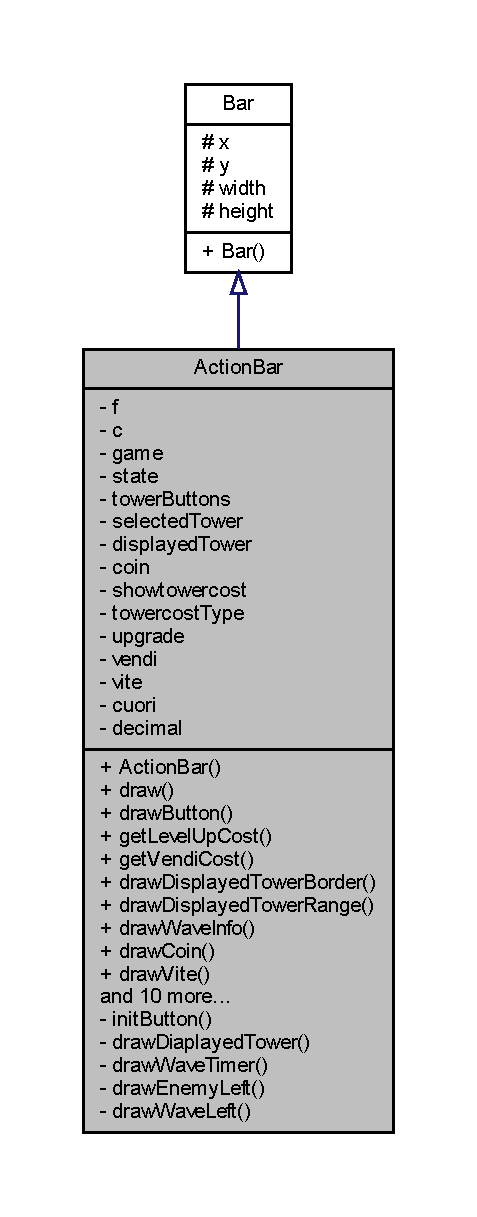
\includegraphics[height=550pt]{classui_1_1_action_bar__inherit__graph}
\end{center}
\end{figure}


Collaboration diagram for Action\+Bar\+:
\nopagebreak
\begin{figure}[H]
\begin{center}
\leavevmode
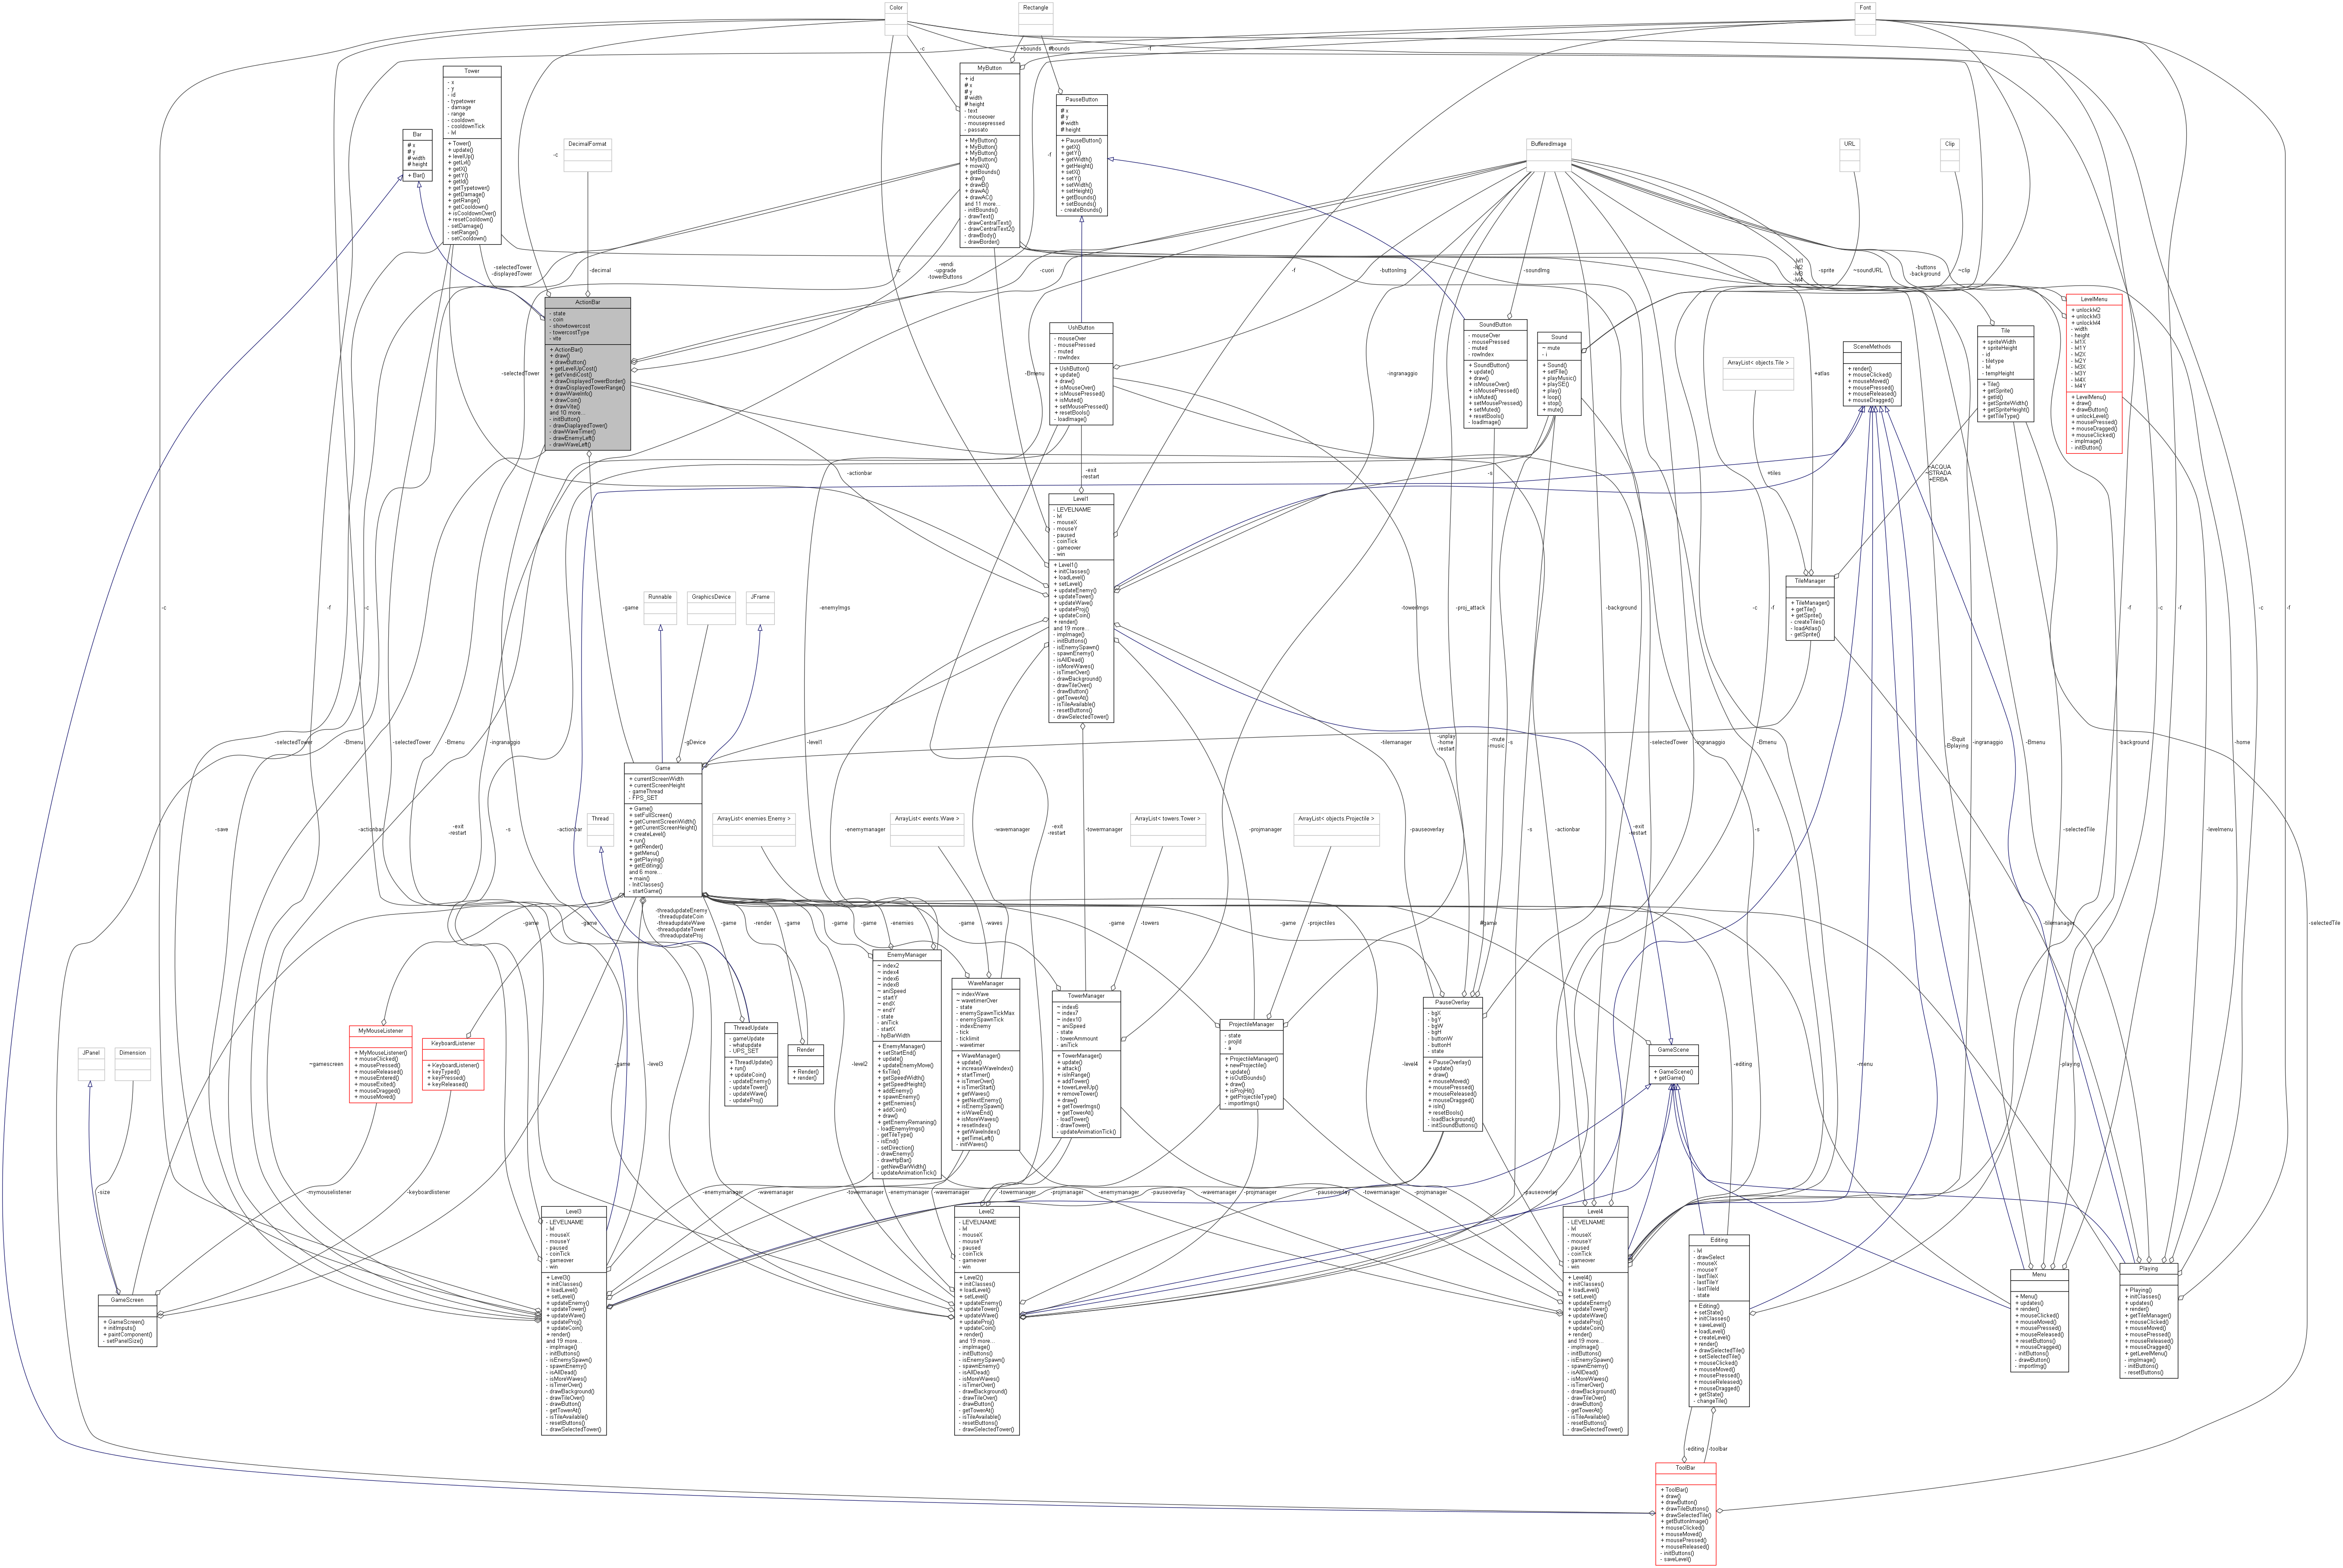
\includegraphics[width=350pt]{classui_1_1_action_bar__coll__graph}
\end{center}
\end{figure}
\subsection*{Public Member Functions}
\begin{DoxyCompactItemize}
\item 
\hyperlink{classui_1_1_action_bar_a4ff9099a9e2976f76bc6d0e2e5041cc6}{Action\+Bar} (int \hyperlink{classui_1_1_bar_a6150e0515f7202e2fb518f7206ed97dc}{x}, int \hyperlink{classui_1_1_bar_a0a2f84ed7838f07779ae24c5a9086d33}{y}, int \hyperlink{classui_1_1_bar_a2474a5474cbff19523a51eb1de01cda4}{width}, int \hyperlink{classui_1_1_bar_ad12fc34ce789bce6c8a05d8a17138534}{height}, \hyperlink{classprogetto_1_1_game}{Game} \hyperlink{classui_1_1_action_bar_ac6a5ed6191fcf3a5bf0445921feb4f48}{game}, String \hyperlink{classui_1_1_action_bar_a91ac952876f776b3fbbc8519e093fdbf}{state})
\begin{DoxyCompactList}\small\item\em costruttore, setta variabili, immagini e bottoni. \end{DoxyCompactList}\item 
void \hyperlink{classui_1_1_action_bar_a72fe1ffca978e99fd16994a10e7f8051}{draw} (Graphics g)
\begin{DoxyCompactList}\small\item\em disegna i bottoni, le info della tower selezionata, i bottoni per modificarla e i cuori. \end{DoxyCompactList}\item 
void \hyperlink{classui_1_1_action_bar_a65768678909bc0512c6cb9780709ad38}{draw\+Button} (Graphics g)
\begin{DoxyCompactList}\small\item\em disegna i bottoni. \end{DoxyCompactList}\item 
int \hyperlink{classui_1_1_action_bar_a6c5f59282a148a0d74bc5aa58d5ad307}{get\+Level\+Up\+Cost} (\hyperlink{classtowers_1_1_tower}{Tower} \hyperlink{classui_1_1_action_bar_a45f9b90370e0d7a88bd448d0c07267a4}{displayed\+Tower})
\begin{DoxyCompactList}\small\item\em restituisce il costo per upgradare la torre selezionata. \end{DoxyCompactList}\item 
int \hyperlink{classui_1_1_action_bar_aef810268cda93505da735c6c81136e00}{get\+Vendi\+Cost} (\hyperlink{classtowers_1_1_tower}{Tower} \hyperlink{classui_1_1_action_bar_a45f9b90370e0d7a88bd448d0c07267a4}{displayed\+Tower})
\begin{DoxyCompactList}\small\item\em restituisce il guadagno della vendita della torre selezionata. \end{DoxyCompactList}\item 
void \hyperlink{classui_1_1_action_bar_a04a438da46ac439f00343a12939ada6e}{draw\+Displayed\+Tower\+Border} (Graphics g)
\begin{DoxyCompactList}\small\item\em disegna i bordi della torre selezionata. \end{DoxyCompactList}\item 
void \hyperlink{classui_1_1_action_bar_a1f012512b669e57c49c1957905a35107}{draw\+Displayed\+Tower\+Range} (Graphics g)
\begin{DoxyCompactList}\small\item\em disegna il cerchio del range di attacco della torre selezionata. \end{DoxyCompactList}\item 
void \hyperlink{classui_1_1_action_bar_a4202926f30a7290c360bfcd4af6b03cb}{draw\+Wave\+Info} (Graphics g)
\begin{DoxyCompactList}\small\item\em disegna le informazioni relative all\textquotesingle{}ondata. \end{DoxyCompactList}\item 
void \hyperlink{classui_1_1_action_bar_ae07c200235fb700738b8194a93dbb8fb}{draw\+Coin} (Graphics g)
\begin{DoxyCompactList}\small\item\em disegna il numero di monete. \end{DoxyCompactList}\item 
void \hyperlink{classui_1_1_action_bar_a7075e1ba9a7135d89d02dca2e3b8860e}{draw\+Vite} (Graphics g)
\begin{DoxyCompactList}\small\item\em disegna le vite. \end{DoxyCompactList}\item 
void \hyperlink{classui_1_1_action_bar_a99a8282ac7383f267261ca608cafe139}{remove\+Coin} (int type)
\begin{DoxyCompactList}\small\item\em rimuove delle monete. \end{DoxyCompactList}\item 
void \hyperlink{classui_1_1_action_bar_a8e9e4227428708da489e0b37223377a8}{add\+Coin} (int \hyperlink{classui_1_1_action_bar_a41de228368d6181324d7bfbdf40875e3}{coin})
\begin{DoxyCompactList}\small\item\em aggiunge delle monete. \end{DoxyCompactList}\item 
void \hyperlink{classui_1_1_action_bar_a32afe6a393c6361d391e26ed96971131}{draw\+Tower\+Cost} (Graphics g)
\begin{DoxyCompactList}\small\item\em disegna il costo della torre da piazzare. \end{DoxyCompactList}\item 
void \hyperlink{classui_1_1_action_bar_aacab7287bc123d863feb4551df131934}{display\+Tower} (\hyperlink{classtowers_1_1_tower}{Tower} t)
\begin{DoxyCompactList}\small\item\em setta la torre da disegnare. \end{DoxyCompactList}\item 
int \hyperlink{classui_1_1_action_bar_a3de978b9745ea5fdbe99d556e40166f6}{get\+Vite} ()
\begin{DoxyCompactList}\small\item\em restituisce il numero di vite. \end{DoxyCompactList}\item 
void \hyperlink{classui_1_1_action_bar_a484775c889ccd8602b66ad795b141534}{rimuovi\+Vita} ()
\begin{DoxyCompactList}\small\item\em rimuove una vita ed eventualmente termina il livello. \end{DoxyCompactList}\item 
void \hyperlink{classui_1_1_action_bar_a45d56bd84238e8b56589dfc732e2b2cf}{mouse\+Clicked} (Mouse\+Event e)
\begin{DoxyCompactList}\small\item\em gestisce i click del mouse. \end{DoxyCompactList}\item 
void \hyperlink{classui_1_1_action_bar_a2ca251710b65639ec80bc141edde60aa}{mouse\+Moved} (Mouse\+Event e)
\begin{DoxyCompactList}\small\item\em gestisce le move del mouse. \end{DoxyCompactList}\item 
void \hyperlink{classui_1_1_action_bar_aed82e1ce3dd3cf283d508c3ba3be70ef}{mouse\+Pressed} (Mouse\+Event e)
\begin{DoxyCompactList}\small\item\em gestisce le press del mouse. \end{DoxyCompactList}\item 
void \hyperlink{classui_1_1_action_bar_a87a07291794e15052db67f945d90853e}{mouse\+Released} (Mouse\+Event e)
\begin{DoxyCompactList}\small\item\em gestisce le release del mouse. \end{DoxyCompactList}\end{DoxyCompactItemize}
\subsection*{Private Member Functions}
\begin{DoxyCompactItemize}
\item 
void \hyperlink{classui_1_1_action_bar_aed9fe7e919d4355a7ad86701d44e1fea}{init\+Button} ()
\begin{DoxyCompactList}\small\item\em inizializza i bottoni. \end{DoxyCompactList}\item 
void \hyperlink{classui_1_1_action_bar_a2177b06de4c0084e953665a7dbfd6772}{draw\+Diaplayed\+Tower} (Graphics g)
\begin{DoxyCompactList}\small\item\em disegna la torre selezionata, le sue info e i bottoni relativi ad essa. \end{DoxyCompactList}\item 
void \hyperlink{classui_1_1_action_bar_a01f37d59ae4977fa55a1a6dd3e8bd543}{draw\+Wave\+Timer} (Graphics g)
\begin{DoxyCompactList}\small\item\em disegna il timer dell\textquotesingle{}ondata. \end{DoxyCompactList}\item 
void \hyperlink{classui_1_1_action_bar_abb1fa26db5a1c2f4b0776a316ad85249}{draw\+Enemy\+Left} (Graphics g)
\begin{DoxyCompactList}\small\item\em disegna il numero di nemici rimanenti. \end{DoxyCompactList}\item 
void \hyperlink{classui_1_1_action_bar_aeb491734ea2c8ae2f1be9db4f930d22a}{draw\+Wave\+Left} (Graphics g)
\begin{DoxyCompactList}\small\item\em disegna il numero dell\textquotesingle{}ondata. \end{DoxyCompactList}\end{DoxyCompactItemize}
\subsection*{Private Attributes}
\begin{DoxyCompactItemize}
\item 
Font \hyperlink{classui_1_1_action_bar_a3fb562f10e8f7f83cb2ed130eab6d439}{f}
\item 
Color \hyperlink{classui_1_1_action_bar_a02094092ae89aa4b23bff1976bcbf90d}{c}
\item 
\hyperlink{classprogetto_1_1_game}{Game} \hyperlink{classui_1_1_action_bar_ac6a5ed6191fcf3a5bf0445921feb4f48}{game}
\item 
String \hyperlink{classui_1_1_action_bar_a91ac952876f776b3fbbc8519e093fdbf}{state}
\item 
\hyperlink{classui_1_1_my_button}{My\+Button} \mbox{[}$\,$\mbox{]} \hyperlink{classui_1_1_action_bar_a6f80c6907b95d4fad643eb5cc2f9c343}{tower\+Buttons}
\item 
\hyperlink{classtowers_1_1_tower}{Tower} \hyperlink{classui_1_1_action_bar_af6b1162bc2f00f8d549aae075ddd5a8b}{selected\+Tower}
\item 
\hyperlink{classtowers_1_1_tower}{Tower} \hyperlink{classui_1_1_action_bar_a45f9b90370e0d7a88bd448d0c07267a4}{displayed\+Tower}
\item 
int \hyperlink{classui_1_1_action_bar_a41de228368d6181324d7bfbdf40875e3}{coin} = 50
\item 
boolean \hyperlink{classui_1_1_action_bar_a520548d3a9dd584072883850aab5a593}{showtowercost}
\item 
int \hyperlink{classui_1_1_action_bar_a62854c85f7998bd19028b0c197e96991}{towercost\+Type}
\item 
\hyperlink{classui_1_1_my_button}{My\+Button} \hyperlink{classui_1_1_action_bar_ad424c422ef61739d7476cfafcb9aba28}{upgrade}
\item 
\hyperlink{classui_1_1_my_button}{My\+Button} \hyperlink{classui_1_1_action_bar_aca046bb433955f594a9af60ab1c34640}{vendi}
\item 
int \hyperlink{classui_1_1_action_bar_ace261aa2e09513de9acfbe08311c0f07}{vite} = 3
\item 
Buffered\+Image \mbox{[}$\,$\mbox{]} \hyperlink{classui_1_1_action_bar_a724d03f52f34297222dd1f423b96b6df}{cuori}
\item 
Decimal\+Format \hyperlink{classui_1_1_action_bar_ab1f373e2f226eeef8843871210341966}{decimal} = new Decimal\+Format(\char`\"{}0.\+0\char`\"{})
\end{DoxyCompactItemize}
\subsection*{Additional Inherited Members}


\subsection{Detailed Description}
classe figlia della classe \char`\"{}\+Bar\char`\"{} per gestire la barra presente nei livelli 

Definition at line 32 of file Action\+Bar.\+java.



\subsection{Constructor \& Destructor Documentation}
\mbox{\Hypertarget{classui_1_1_action_bar_a4ff9099a9e2976f76bc6d0e2e5041cc6}\label{classui_1_1_action_bar_a4ff9099a9e2976f76bc6d0e2e5041cc6}} 
\index{ui\+::\+Action\+Bar@{ui\+::\+Action\+Bar}!Action\+Bar@{Action\+Bar}}
\index{Action\+Bar@{Action\+Bar}!ui\+::\+Action\+Bar@{ui\+::\+Action\+Bar}}
\subsubsection{\texorpdfstring{Action\+Bar()}{ActionBar()}}
{\footnotesize\ttfamily \hyperlink{classui_1_1_action_bar}{Action\+Bar} (\begin{DoxyParamCaption}\item[{int}]{x,  }\item[{int}]{y,  }\item[{int}]{width,  }\item[{int}]{height,  }\item[{\hyperlink{classprogetto_1_1_game}{Game}}]{game,  }\item[{String}]{state }\end{DoxyParamCaption})}



costruttore, setta variabili, immagini e bottoni. 


\begin{DoxyParams}{Parameters}
{\em x} & coordinata \\
\hline
{\em y} & coordinata \\
\hline
{\em width} & larghezza \\
\hline
{\em height} & altezza \\
\hline
{\em game} & oggetto del gioco \\
\hline
{\em state} & stato dal quale viene invocata l\textquotesingle{}action bar \\
\hline
\end{DoxyParams}


Definition at line 86 of file Action\+Bar.\+java.

Here is the call graph for this function\+:\nopagebreak
\begin{figure}[H]
\begin{center}
\leavevmode
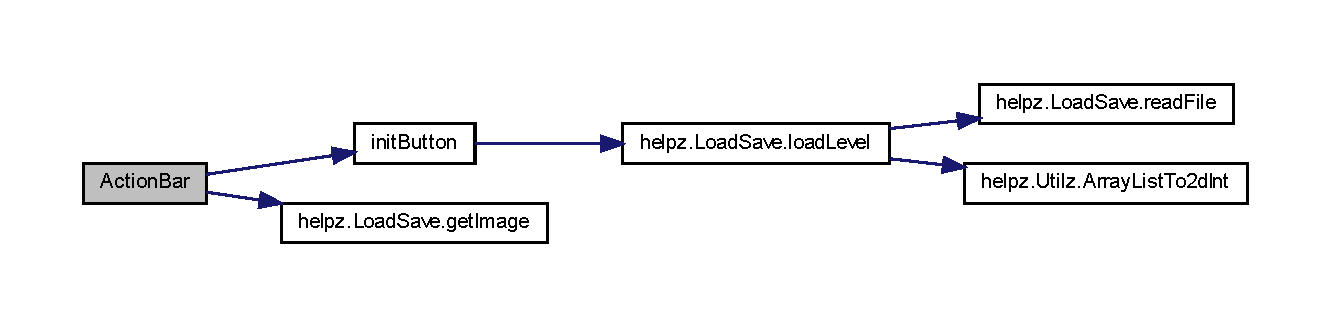
\includegraphics[width=350pt]{classui_1_1_action_bar_a4ff9099a9e2976f76bc6d0e2e5041cc6_cgraph}
\end{center}
\end{figure}


\subsection{Member Function Documentation}
\mbox{\Hypertarget{classui_1_1_action_bar_a8e9e4227428708da489e0b37223377a8}\label{classui_1_1_action_bar_a8e9e4227428708da489e0b37223377a8}} 
\index{ui\+::\+Action\+Bar@{ui\+::\+Action\+Bar}!add\+Coin@{add\+Coin}}
\index{add\+Coin@{add\+Coin}!ui\+::\+Action\+Bar@{ui\+::\+Action\+Bar}}
\subsubsection{\texorpdfstring{add\+Coin()}{addCoin()}}
{\footnotesize\ttfamily void add\+Coin (\begin{DoxyParamCaption}\item[{int}]{coin }\end{DoxyParamCaption})}



aggiunge delle monete. 


\begin{DoxyParams}{Parameters}
{\em coin} & numero di monete da aggiungere \\
\hline
\end{DoxyParams}


Definition at line 446 of file Action\+Bar.\+java.

Here is the caller graph for this function\+:\nopagebreak
\begin{figure}[H]
\begin{center}
\leavevmode
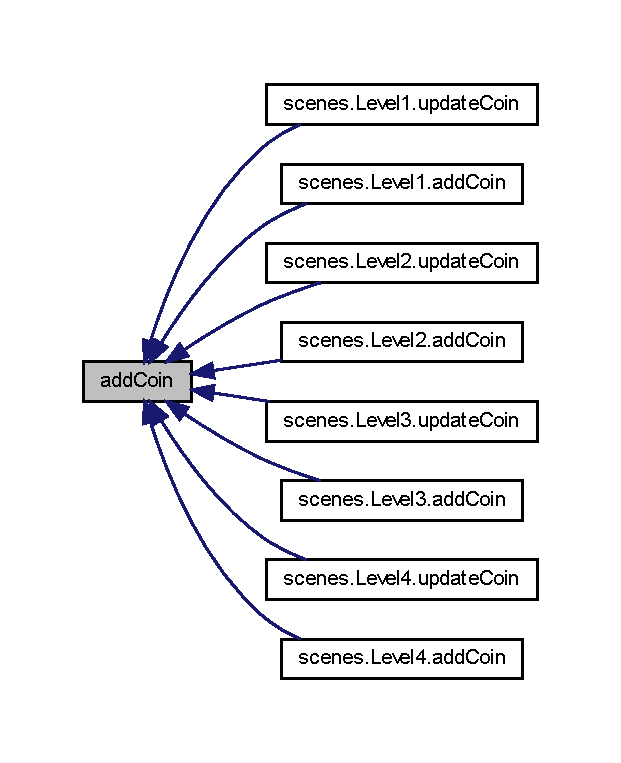
\includegraphics[width=298pt]{classui_1_1_action_bar_a8e9e4227428708da489e0b37223377a8_icgraph}
\end{center}
\end{figure}
\mbox{\Hypertarget{classui_1_1_action_bar_aacab7287bc123d863feb4551df131934}\label{classui_1_1_action_bar_aacab7287bc123d863feb4551df131934}} 
\index{ui\+::\+Action\+Bar@{ui\+::\+Action\+Bar}!display\+Tower@{display\+Tower}}
\index{display\+Tower@{display\+Tower}!ui\+::\+Action\+Bar@{ui\+::\+Action\+Bar}}
\subsubsection{\texorpdfstring{display\+Tower()}{displayTower()}}
{\footnotesize\ttfamily void display\+Tower (\begin{DoxyParamCaption}\item[{\hyperlink{classtowers_1_1_tower}{Tower}}]{t }\end{DoxyParamCaption})}



setta la torre da disegnare. 


\begin{DoxyParams}{Parameters}
{\em t} & torre da disegnare \\
\hline
\end{DoxyParams}


Definition at line 479 of file Action\+Bar.\+java.

Here is the caller graph for this function\+:\nopagebreak
\begin{figure}[H]
\begin{center}
\leavevmode
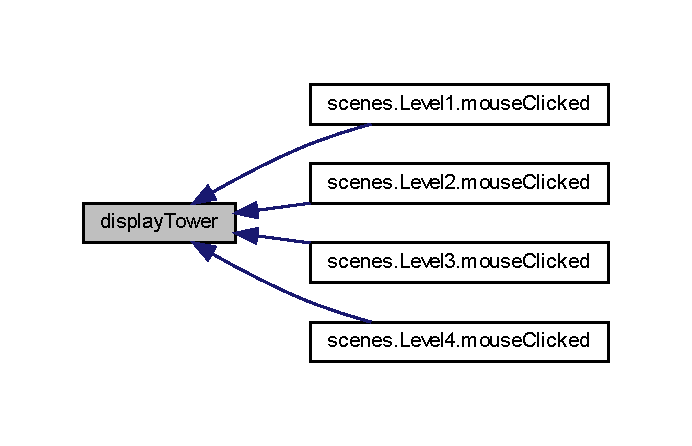
\includegraphics[width=332pt]{classui_1_1_action_bar_aacab7287bc123d863feb4551df131934_icgraph}
\end{center}
\end{figure}
\mbox{\Hypertarget{classui_1_1_action_bar_a72fe1ffca978e99fd16994a10e7f8051}\label{classui_1_1_action_bar_a72fe1ffca978e99fd16994a10e7f8051}} 
\index{ui\+::\+Action\+Bar@{ui\+::\+Action\+Bar}!draw@{draw}}
\index{draw@{draw}!ui\+::\+Action\+Bar@{ui\+::\+Action\+Bar}}
\subsubsection{\texorpdfstring{draw()}{draw()}}
{\footnotesize\ttfamily void draw (\begin{DoxyParamCaption}\item[{Graphics}]{g }\end{DoxyParamCaption})}



disegna i bottoni, le info della tower selezionata, i bottoni per modificarla e i cuori. 


\begin{DoxyParams}{Parameters}
{\em g} & oggetto della grafica \\
\hline
\end{DoxyParams}


Definition at line 132 of file Action\+Bar.\+java.

Here is the call graph for this function\+:\nopagebreak
\begin{figure}[H]
\begin{center}
\leavevmode
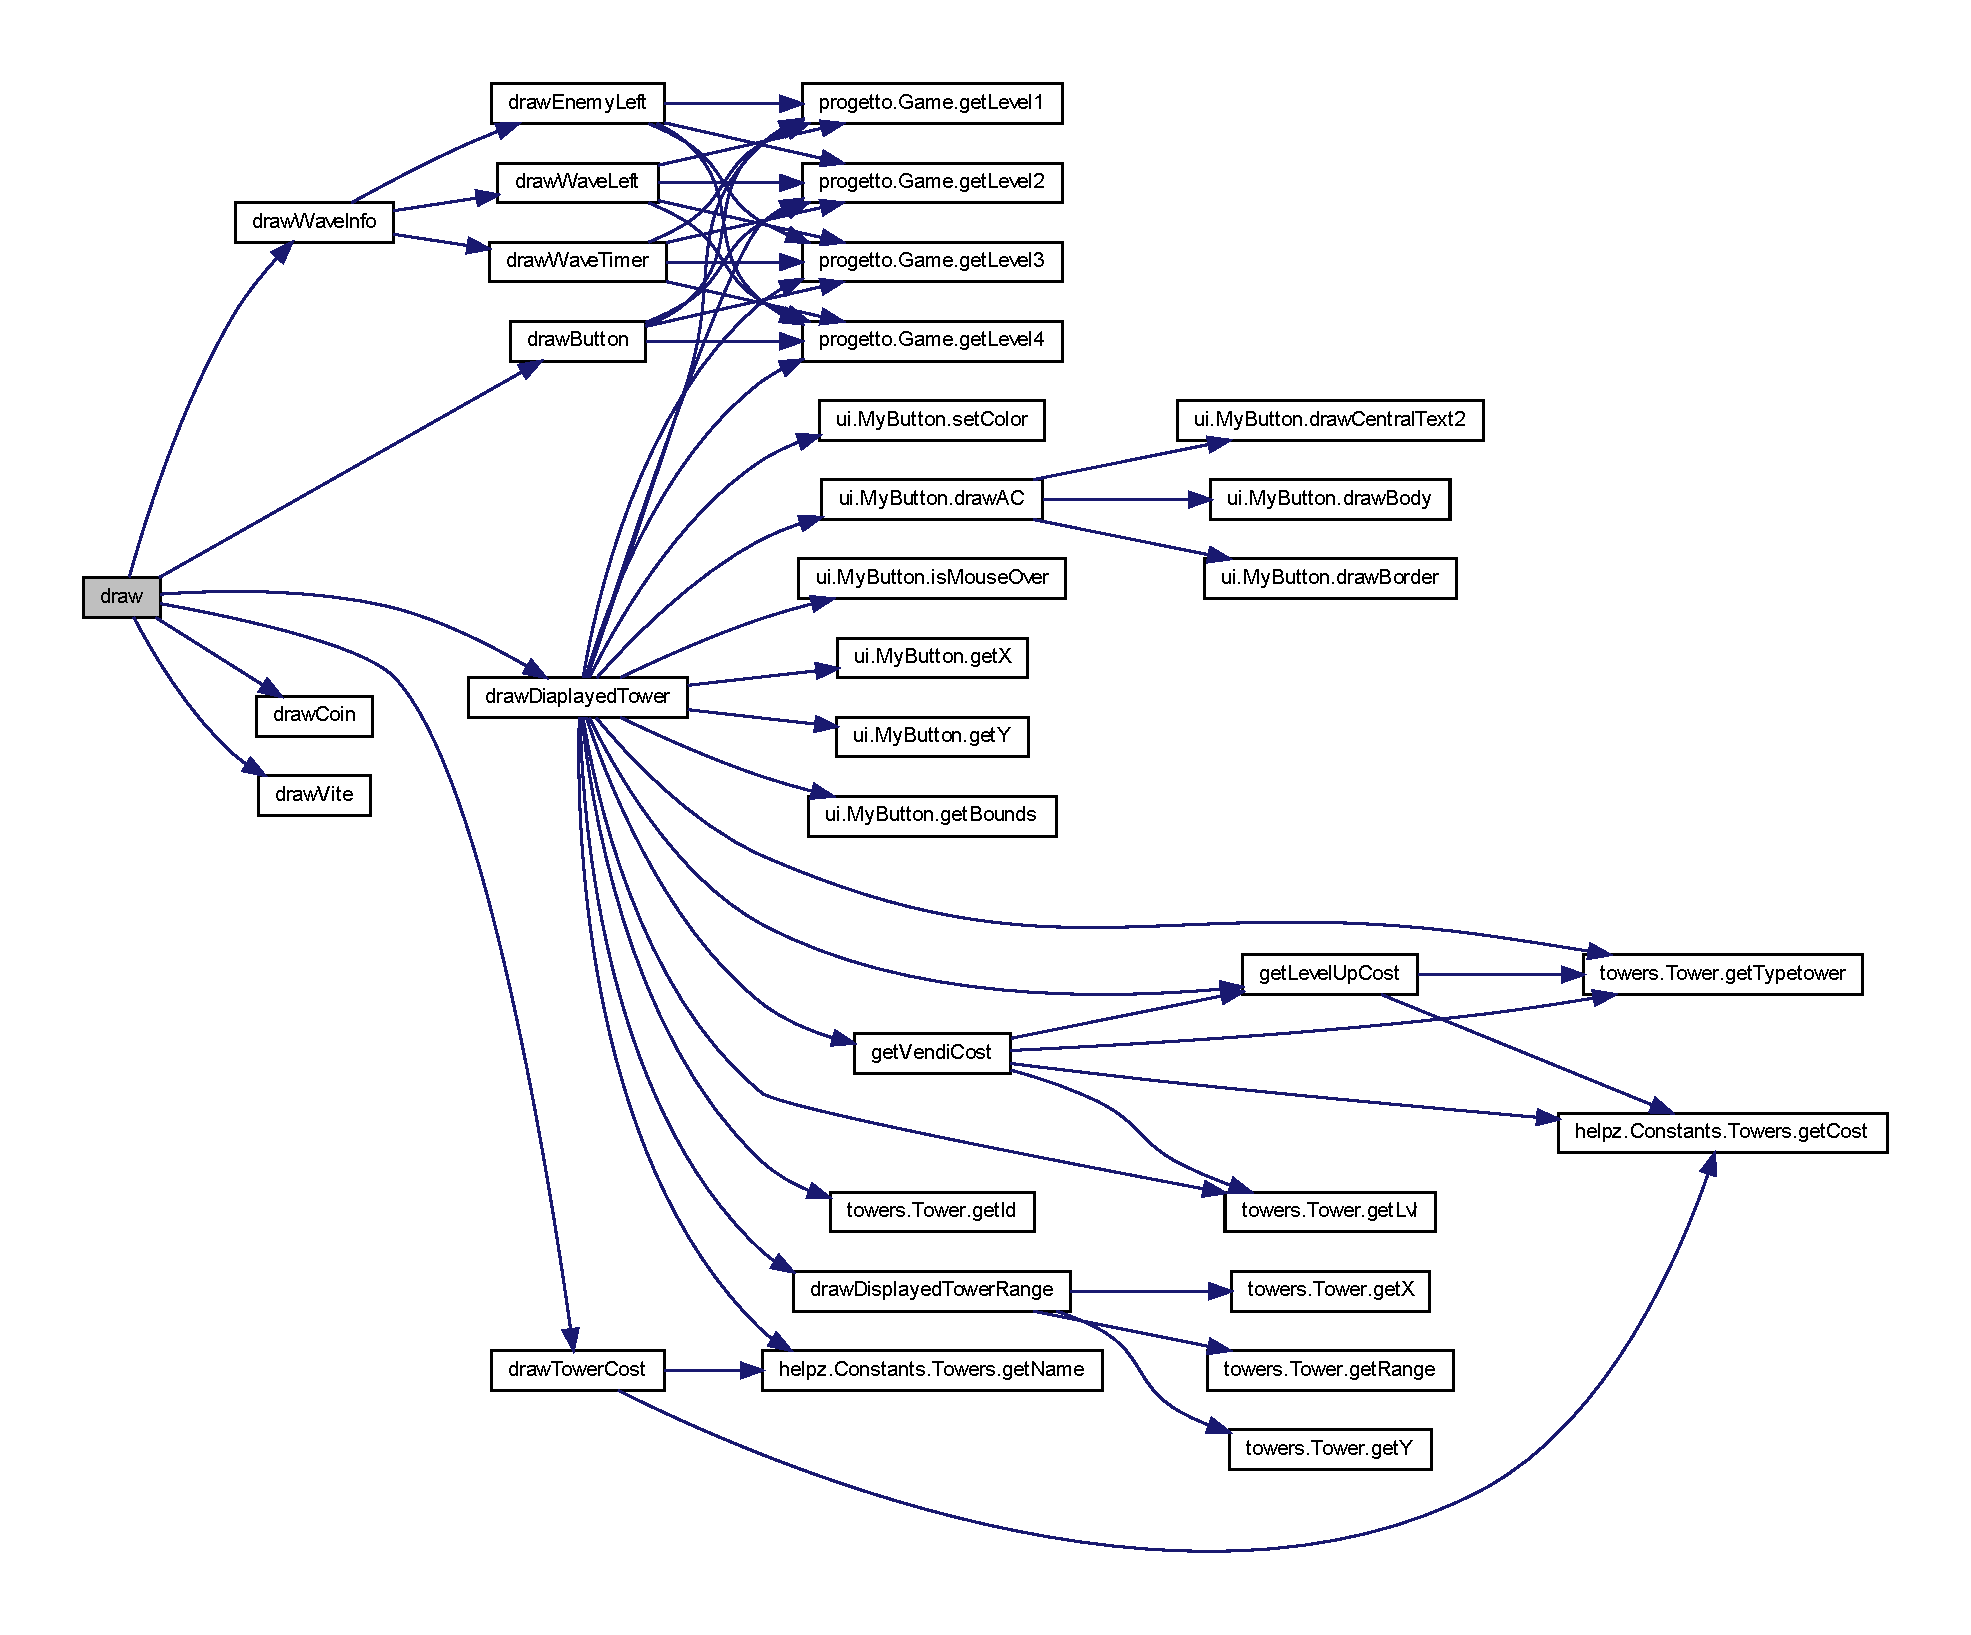
\includegraphics[width=350pt]{classui_1_1_action_bar_a72fe1ffca978e99fd16994a10e7f8051_cgraph}
\end{center}
\end{figure}
Here is the caller graph for this function\+:\nopagebreak
\begin{figure}[H]
\begin{center}
\leavevmode
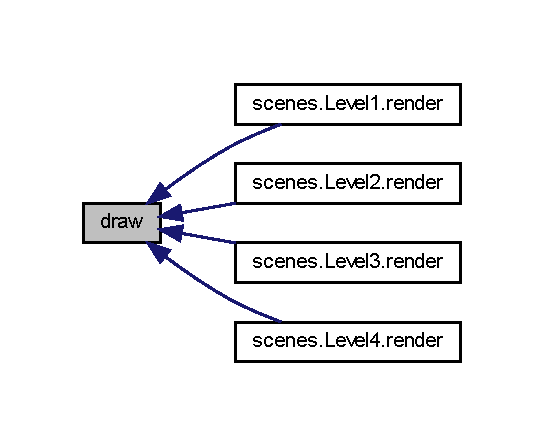
\includegraphics[width=261pt]{classui_1_1_action_bar_a72fe1ffca978e99fd16994a10e7f8051_icgraph}
\end{center}
\end{figure}
\mbox{\Hypertarget{classui_1_1_action_bar_a65768678909bc0512c6cb9780709ad38}\label{classui_1_1_action_bar_a65768678909bc0512c6cb9780709ad38}} 
\index{ui\+::\+Action\+Bar@{ui\+::\+Action\+Bar}!draw\+Button@{draw\+Button}}
\index{draw\+Button@{draw\+Button}!ui\+::\+Action\+Bar@{ui\+::\+Action\+Bar}}
\subsubsection{\texorpdfstring{draw\+Button()}{drawButton()}}
{\footnotesize\ttfamily void draw\+Button (\begin{DoxyParamCaption}\item[{Graphics}]{g }\end{DoxyParamCaption})}



disegna i bottoni. 


\begin{DoxyParams}{Parameters}
{\em g} & oggetto della grafica \\
\hline
\end{DoxyParams}


Definition at line 160 of file Action\+Bar.\+java.

Here is the call graph for this function\+:\nopagebreak
\begin{figure}[H]
\begin{center}
\leavevmode
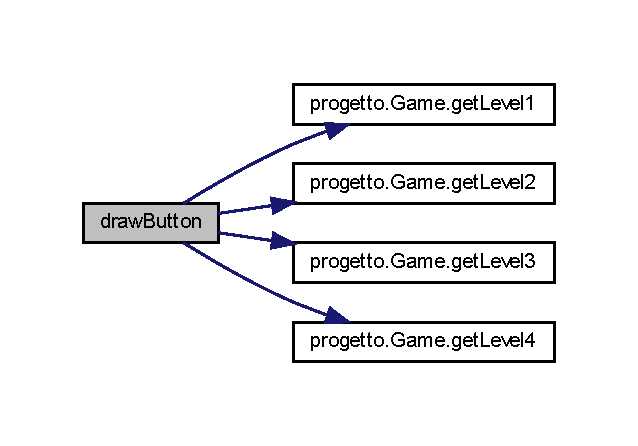
\includegraphics[width=306pt]{classui_1_1_action_bar_a65768678909bc0512c6cb9780709ad38_cgraph}
\end{center}
\end{figure}
Here is the caller graph for this function\+:\nopagebreak
\begin{figure}[H]
\begin{center}
\leavevmode
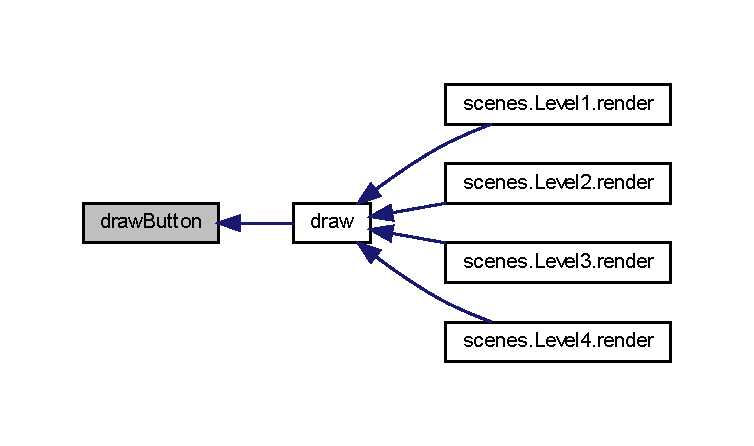
\includegraphics[width=350pt]{classui_1_1_action_bar_a65768678909bc0512c6cb9780709ad38_icgraph}
\end{center}
\end{figure}
\mbox{\Hypertarget{classui_1_1_action_bar_ae07c200235fb700738b8194a93dbb8fb}\label{classui_1_1_action_bar_ae07c200235fb700738b8194a93dbb8fb}} 
\index{ui\+::\+Action\+Bar@{ui\+::\+Action\+Bar}!draw\+Coin@{draw\+Coin}}
\index{draw\+Coin@{draw\+Coin}!ui\+::\+Action\+Bar@{ui\+::\+Action\+Bar}}
\subsubsection{\texorpdfstring{draw\+Coin()}{drawCoin()}}
{\footnotesize\ttfamily void draw\+Coin (\begin{DoxyParamCaption}\item[{Graphics}]{g }\end{DoxyParamCaption})}



disegna il numero di monete. 


\begin{DoxyParams}{Parameters}
{\em g} & oggetto della grafica \\
\hline
\end{DoxyParams}


Definition at line 393 of file Action\+Bar.\+java.

Here is the caller graph for this function\+:\nopagebreak
\begin{figure}[H]
\begin{center}
\leavevmode
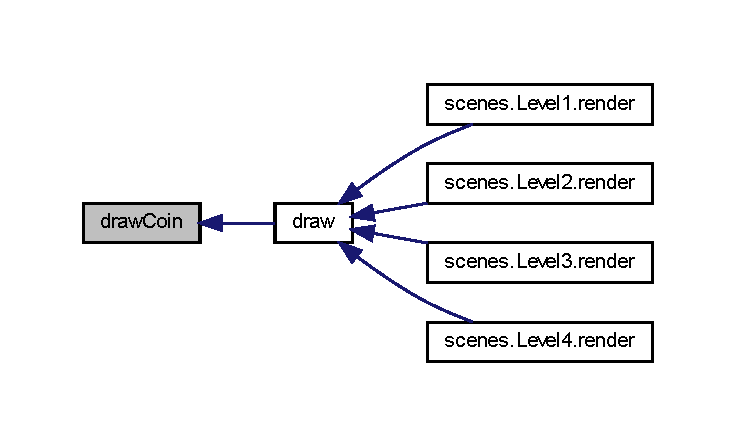
\includegraphics[width=350pt]{classui_1_1_action_bar_ae07c200235fb700738b8194a93dbb8fb_icgraph}
\end{center}
\end{figure}
\mbox{\Hypertarget{classui_1_1_action_bar_a2177b06de4c0084e953665a7dbfd6772}\label{classui_1_1_action_bar_a2177b06de4c0084e953665a7dbfd6772}} 
\index{ui\+::\+Action\+Bar@{ui\+::\+Action\+Bar}!draw\+Diaplayed\+Tower@{draw\+Diaplayed\+Tower}}
\index{draw\+Diaplayed\+Tower@{draw\+Diaplayed\+Tower}!ui\+::\+Action\+Bar@{ui\+::\+Action\+Bar}}
\subsubsection{\texorpdfstring{draw\+Diaplayed\+Tower()}{drawDiaplayedTower()}}
{\footnotesize\ttfamily void draw\+Diaplayed\+Tower (\begin{DoxyParamCaption}\item[{Graphics}]{g }\end{DoxyParamCaption})\hspace{0.3cm}{\ttfamily [private]}}



disegna la torre selezionata, le sue info e i bottoni relativi ad essa. 


\begin{DoxyParams}{Parameters}
{\em g} & oggetto della grafica \\
\hline
\end{DoxyParams}


Definition at line 186 of file Action\+Bar.\+java.

Here is the call graph for this function\+:\nopagebreak
\begin{figure}[H]
\begin{center}
\leavevmode
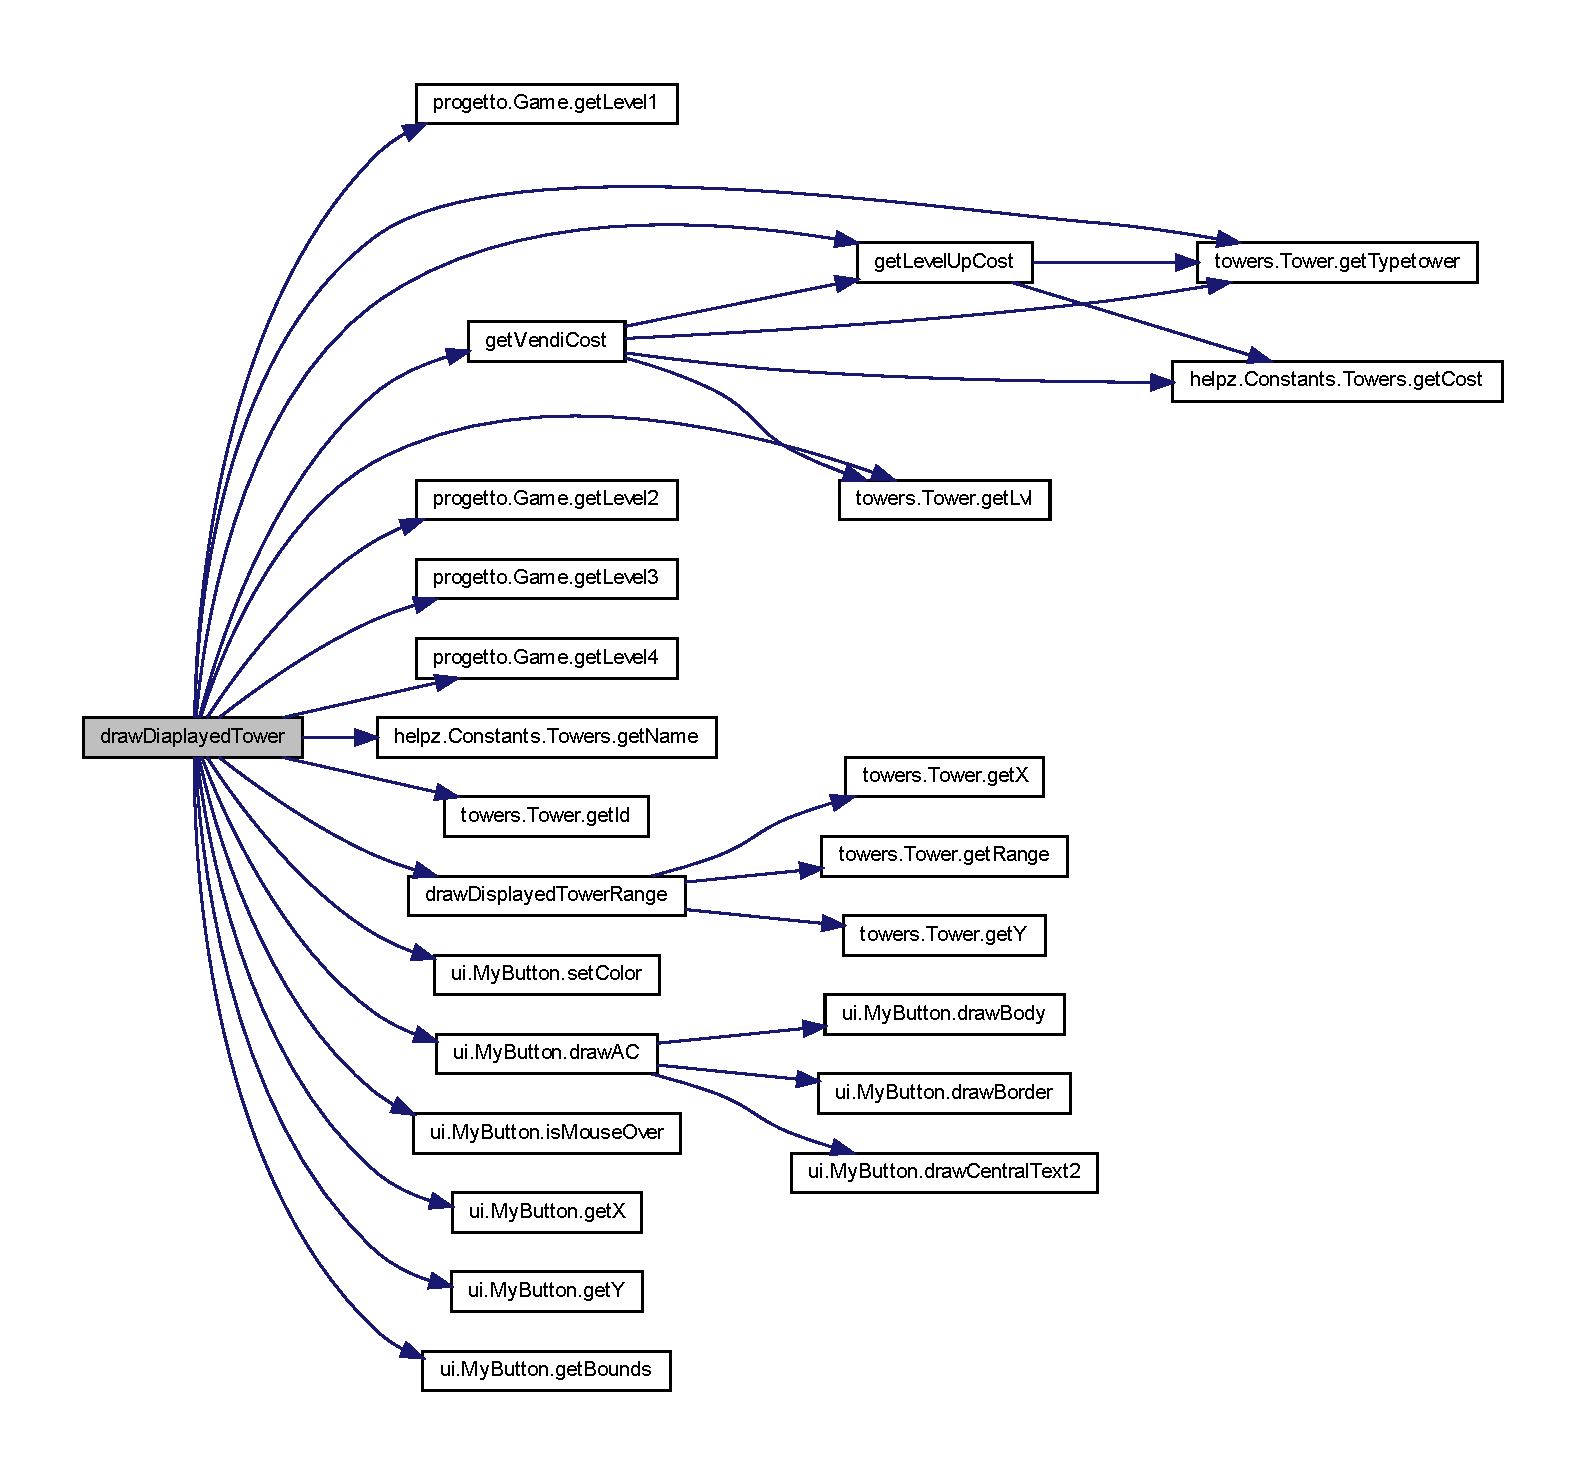
\includegraphics[width=350pt]{classui_1_1_action_bar_a2177b06de4c0084e953665a7dbfd6772_cgraph}
\end{center}
\end{figure}
Here is the caller graph for this function\+:\nopagebreak
\begin{figure}[H]
\begin{center}
\leavevmode
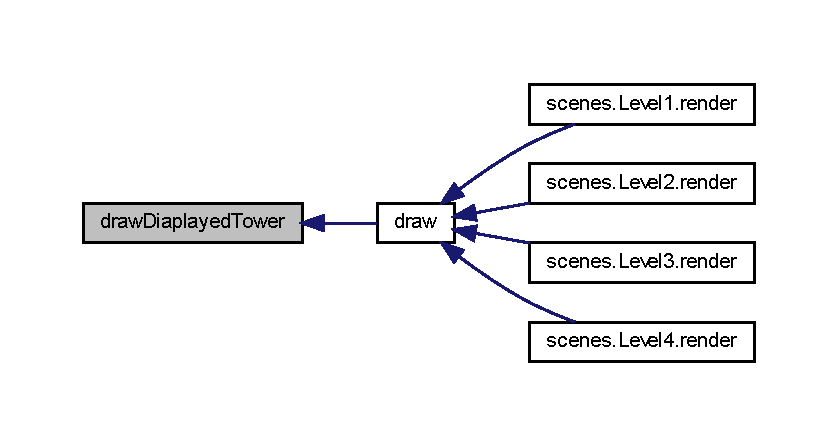
\includegraphics[width=350pt]{classui_1_1_action_bar_a2177b06de4c0084e953665a7dbfd6772_icgraph}
\end{center}
\end{figure}
\mbox{\Hypertarget{classui_1_1_action_bar_a04a438da46ac439f00343a12939ada6e}\label{classui_1_1_action_bar_a04a438da46ac439f00343a12939ada6e}} 
\index{ui\+::\+Action\+Bar@{ui\+::\+Action\+Bar}!draw\+Displayed\+Tower\+Border@{draw\+Displayed\+Tower\+Border}}
\index{draw\+Displayed\+Tower\+Border@{draw\+Displayed\+Tower\+Border}!ui\+::\+Action\+Bar@{ui\+::\+Action\+Bar}}
\subsubsection{\texorpdfstring{draw\+Displayed\+Tower\+Border()}{drawDisplayedTowerBorder()}}
{\footnotesize\ttfamily void draw\+Displayed\+Tower\+Border (\begin{DoxyParamCaption}\item[{Graphics}]{g }\end{DoxyParamCaption})}



disegna i bordi della torre selezionata. 


\begin{DoxyParams}{Parameters}
{\em g} & oggetto della grafica \\
\hline
\end{DoxyParams}


Definition at line 264 of file Action\+Bar.\+java.

Here is the call graph for this function\+:\nopagebreak
\begin{figure}[H]
\begin{center}
\leavevmode
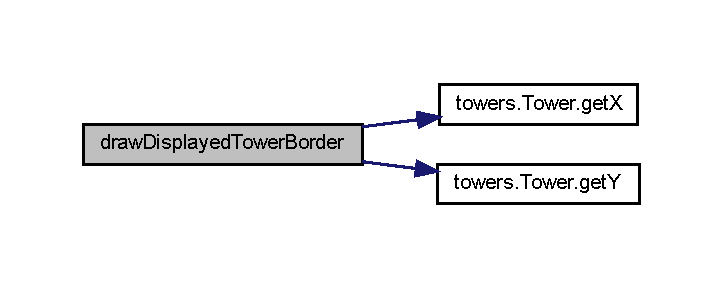
\includegraphics[width=347pt]{classui_1_1_action_bar_a04a438da46ac439f00343a12939ada6e_cgraph}
\end{center}
\end{figure}
\mbox{\Hypertarget{classui_1_1_action_bar_a1f012512b669e57c49c1957905a35107}\label{classui_1_1_action_bar_a1f012512b669e57c49c1957905a35107}} 
\index{ui\+::\+Action\+Bar@{ui\+::\+Action\+Bar}!draw\+Displayed\+Tower\+Range@{draw\+Displayed\+Tower\+Range}}
\index{draw\+Displayed\+Tower\+Range@{draw\+Displayed\+Tower\+Range}!ui\+::\+Action\+Bar@{ui\+::\+Action\+Bar}}
\subsubsection{\texorpdfstring{draw\+Displayed\+Tower\+Range()}{drawDisplayedTowerRange()}}
{\footnotesize\ttfamily void draw\+Displayed\+Tower\+Range (\begin{DoxyParamCaption}\item[{Graphics}]{g }\end{DoxyParamCaption})}



disegna il cerchio del range di attacco della torre selezionata. 


\begin{DoxyParams}{Parameters}
{\em g} & oggetto della grafica \\
\hline
\end{DoxyParams}


Definition at line 274 of file Action\+Bar.\+java.

Here is the call graph for this function\+:\nopagebreak
\begin{figure}[H]
\begin{center}
\leavevmode
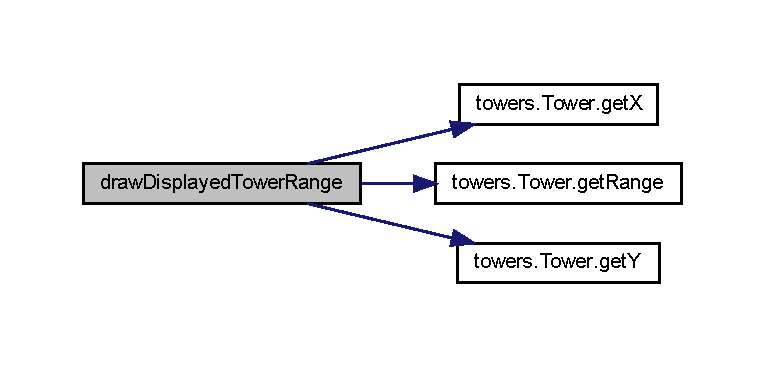
\includegraphics[width=350pt]{classui_1_1_action_bar_a1f012512b669e57c49c1957905a35107_cgraph}
\end{center}
\end{figure}
Here is the caller graph for this function\+:\nopagebreak
\begin{figure}[H]
\begin{center}
\leavevmode
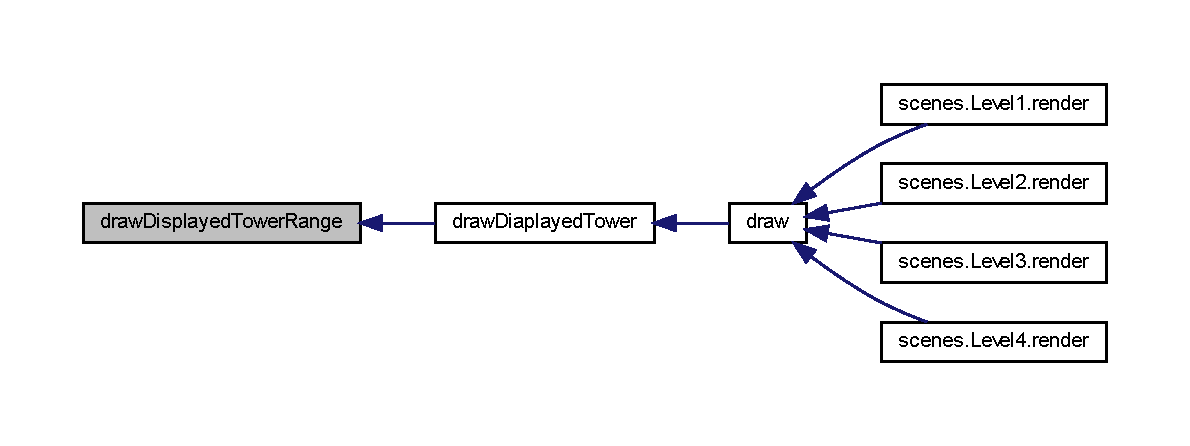
\includegraphics[width=350pt]{classui_1_1_action_bar_a1f012512b669e57c49c1957905a35107_icgraph}
\end{center}
\end{figure}
\mbox{\Hypertarget{classui_1_1_action_bar_abb1fa26db5a1c2f4b0776a316ad85249}\label{classui_1_1_action_bar_abb1fa26db5a1c2f4b0776a316ad85249}} 
\index{ui\+::\+Action\+Bar@{ui\+::\+Action\+Bar}!draw\+Enemy\+Left@{draw\+Enemy\+Left}}
\index{draw\+Enemy\+Left@{draw\+Enemy\+Left}!ui\+::\+Action\+Bar@{ui\+::\+Action\+Bar}}
\subsubsection{\texorpdfstring{draw\+Enemy\+Left()}{drawEnemyLeft()}}
{\footnotesize\ttfamily void draw\+Enemy\+Left (\begin{DoxyParamCaption}\item[{Graphics}]{g }\end{DoxyParamCaption})\hspace{0.3cm}{\ttfamily [private]}}



disegna il numero di nemici rimanenti. 


\begin{DoxyParams}{Parameters}
{\em g} & oggetto della grafica \\
\hline
\end{DoxyParams}


Definition at line 332 of file Action\+Bar.\+java.

Here is the call graph for this function\+:\nopagebreak
\begin{figure}[H]
\begin{center}
\leavevmode
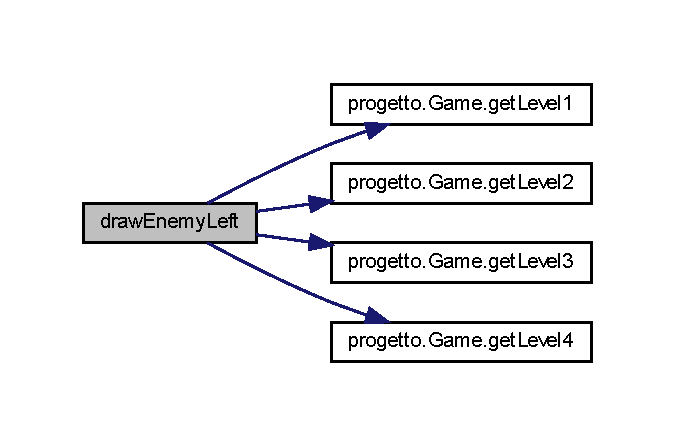
\includegraphics[width=324pt]{classui_1_1_action_bar_abb1fa26db5a1c2f4b0776a316ad85249_cgraph}
\end{center}
\end{figure}
Here is the caller graph for this function\+:\nopagebreak
\begin{figure}[H]
\begin{center}
\leavevmode
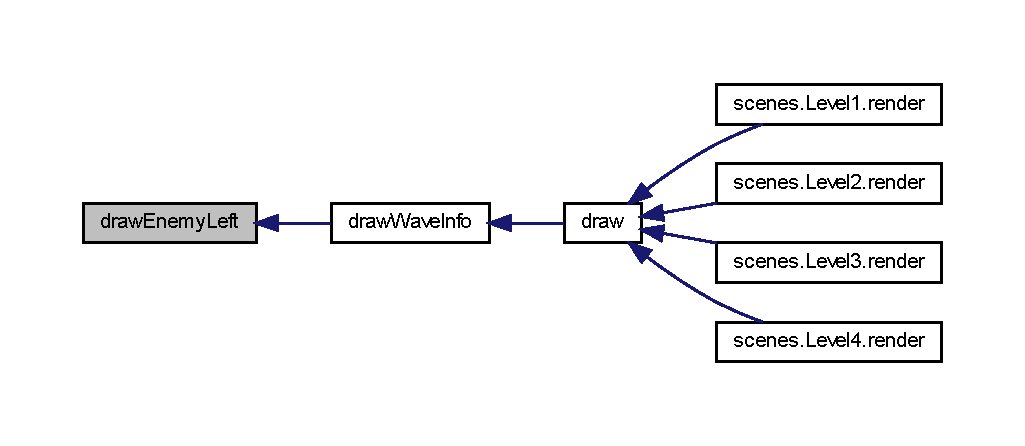
\includegraphics[width=350pt]{classui_1_1_action_bar_abb1fa26db5a1c2f4b0776a316ad85249_icgraph}
\end{center}
\end{figure}
\mbox{\Hypertarget{classui_1_1_action_bar_a32afe6a393c6361d391e26ed96971131}\label{classui_1_1_action_bar_a32afe6a393c6361d391e26ed96971131}} 
\index{ui\+::\+Action\+Bar@{ui\+::\+Action\+Bar}!draw\+Tower\+Cost@{draw\+Tower\+Cost}}
\index{draw\+Tower\+Cost@{draw\+Tower\+Cost}!ui\+::\+Action\+Bar@{ui\+::\+Action\+Bar}}
\subsubsection{\texorpdfstring{draw\+Tower\+Cost()}{drawTowerCost()}}
{\footnotesize\ttfamily void draw\+Tower\+Cost (\begin{DoxyParamCaption}\item[{Graphics}]{g }\end{DoxyParamCaption})}



disegna il costo della torre da piazzare. 


\begin{DoxyParams}{Parameters}
{\em g} & oggetto della grafica \\
\hline
\end{DoxyParams}


Definition at line 455 of file Action\+Bar.\+java.

Here is the call graph for this function\+:\nopagebreak
\begin{figure}[H]
\begin{center}
\leavevmode
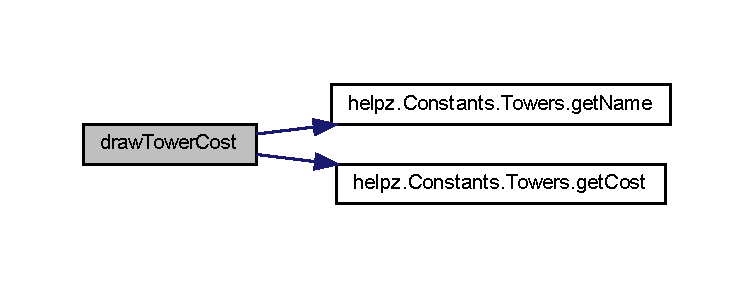
\includegraphics[width=350pt]{classui_1_1_action_bar_a32afe6a393c6361d391e26ed96971131_cgraph}
\end{center}
\end{figure}
Here is the caller graph for this function\+:\nopagebreak
\begin{figure}[H]
\begin{center}
\leavevmode
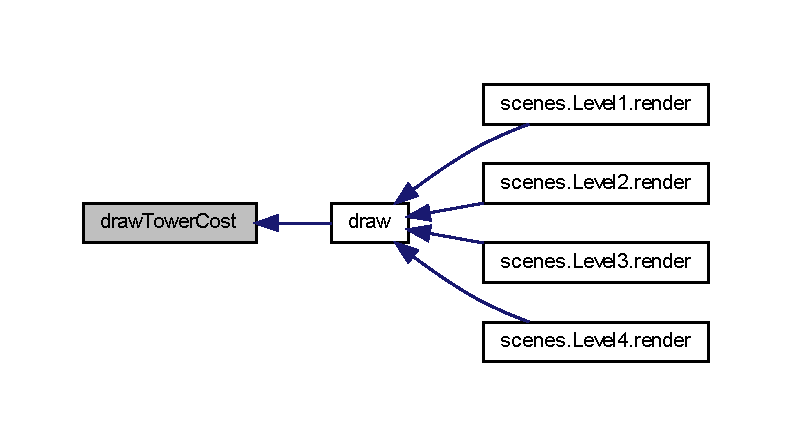
\includegraphics[width=350pt]{classui_1_1_action_bar_a32afe6a393c6361d391e26ed96971131_icgraph}
\end{center}
\end{figure}
\mbox{\Hypertarget{classui_1_1_action_bar_a7075e1ba9a7135d89d02dca2e3b8860e}\label{classui_1_1_action_bar_a7075e1ba9a7135d89d02dca2e3b8860e}} 
\index{ui\+::\+Action\+Bar@{ui\+::\+Action\+Bar}!draw\+Vite@{draw\+Vite}}
\index{draw\+Vite@{draw\+Vite}!ui\+::\+Action\+Bar@{ui\+::\+Action\+Bar}}
\subsubsection{\texorpdfstring{draw\+Vite()}{drawVite()}}
{\footnotesize\ttfamily void draw\+Vite (\begin{DoxyParamCaption}\item[{Graphics}]{g }\end{DoxyParamCaption})}



disegna le vite. 


\begin{DoxyParams}{Parameters}
{\em g} & oggetto della grafica \\
\hline
\end{DoxyParams}


Definition at line 404 of file Action\+Bar.\+java.

Here is the caller graph for this function\+:\nopagebreak
\begin{figure}[H]
\begin{center}
\leavevmode
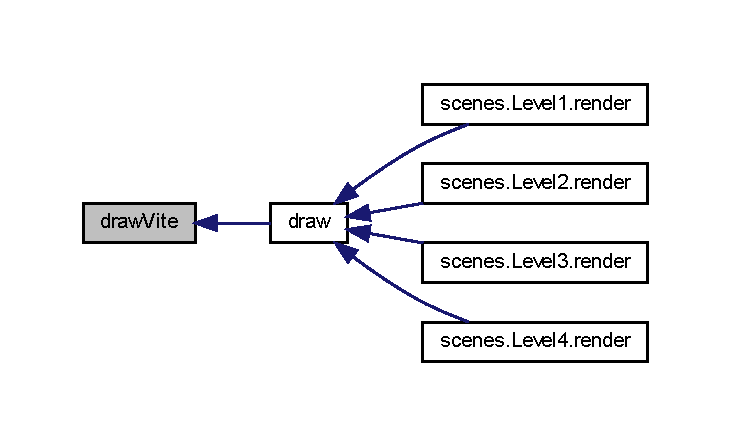
\includegraphics[width=350pt]{classui_1_1_action_bar_a7075e1ba9a7135d89d02dca2e3b8860e_icgraph}
\end{center}
\end{figure}
\mbox{\Hypertarget{classui_1_1_action_bar_a4202926f30a7290c360bfcd4af6b03cb}\label{classui_1_1_action_bar_a4202926f30a7290c360bfcd4af6b03cb}} 
\index{ui\+::\+Action\+Bar@{ui\+::\+Action\+Bar}!draw\+Wave\+Info@{draw\+Wave\+Info}}
\index{draw\+Wave\+Info@{draw\+Wave\+Info}!ui\+::\+Action\+Bar@{ui\+::\+Action\+Bar}}
\subsubsection{\texorpdfstring{draw\+Wave\+Info()}{drawWaveInfo()}}
{\footnotesize\ttfamily void draw\+Wave\+Info (\begin{DoxyParamCaption}\item[{Graphics}]{g }\end{DoxyParamCaption})}



disegna le informazioni relative all\textquotesingle{}ondata. 


\begin{DoxyParams}{Parameters}
{\em g} & oggetto della grafica \\
\hline
\end{DoxyParams}


Definition at line 284 of file Action\+Bar.\+java.

Here is the call graph for this function\+:\nopagebreak
\begin{figure}[H]
\begin{center}
\leavevmode
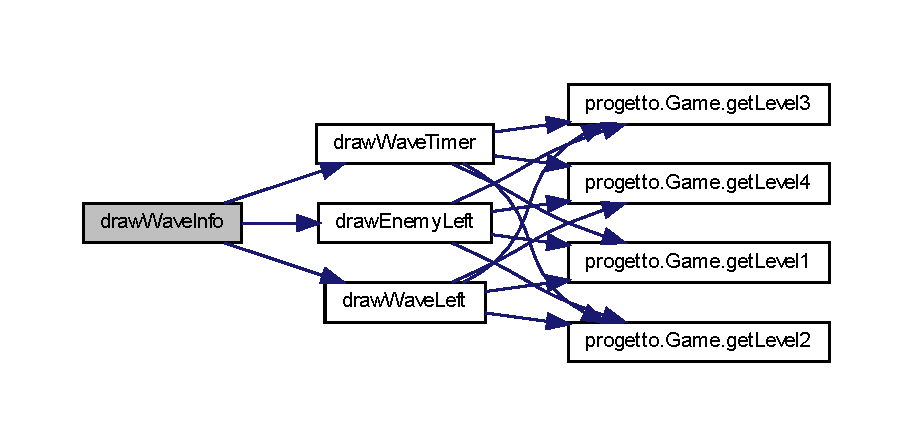
\includegraphics[width=350pt]{classui_1_1_action_bar_a4202926f30a7290c360bfcd4af6b03cb_cgraph}
\end{center}
\end{figure}
Here is the caller graph for this function\+:\nopagebreak
\begin{figure}[H]
\begin{center}
\leavevmode
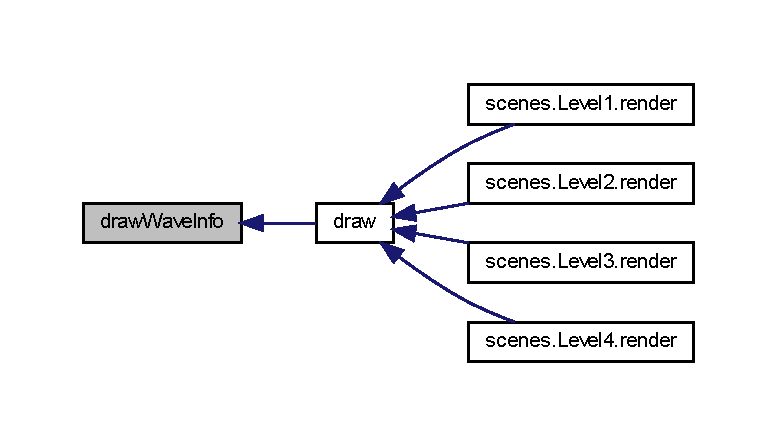
\includegraphics[width=350pt]{classui_1_1_action_bar_a4202926f30a7290c360bfcd4af6b03cb_icgraph}
\end{center}
\end{figure}
\mbox{\Hypertarget{classui_1_1_action_bar_aeb491734ea2c8ae2f1be9db4f930d22a}\label{classui_1_1_action_bar_aeb491734ea2c8ae2f1be9db4f930d22a}} 
\index{ui\+::\+Action\+Bar@{ui\+::\+Action\+Bar}!draw\+Wave\+Left@{draw\+Wave\+Left}}
\index{draw\+Wave\+Left@{draw\+Wave\+Left}!ui\+::\+Action\+Bar@{ui\+::\+Action\+Bar}}
\subsubsection{\texorpdfstring{draw\+Wave\+Left()}{drawWaveLeft()}}
{\footnotesize\ttfamily void draw\+Wave\+Left (\begin{DoxyParamCaption}\item[{Graphics}]{g }\end{DoxyParamCaption})\hspace{0.3cm}{\ttfamily [private]}}



disegna il numero dell\textquotesingle{}ondata. 


\begin{DoxyParams}{Parameters}
{\em g} & oggetto della grafica \\
\hline
\end{DoxyParams}


Definition at line 365 of file Action\+Bar.\+java.

Here is the call graph for this function\+:\nopagebreak
\begin{figure}[H]
\begin{center}
\leavevmode
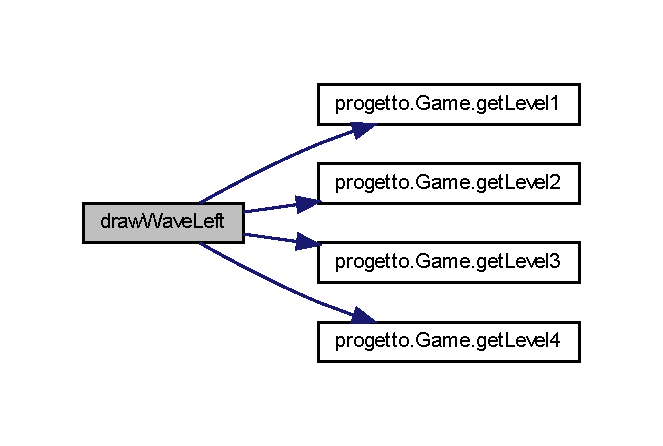
\includegraphics[width=318pt]{classui_1_1_action_bar_aeb491734ea2c8ae2f1be9db4f930d22a_cgraph}
\end{center}
\end{figure}
Here is the caller graph for this function\+:\nopagebreak
\begin{figure}[H]
\begin{center}
\leavevmode
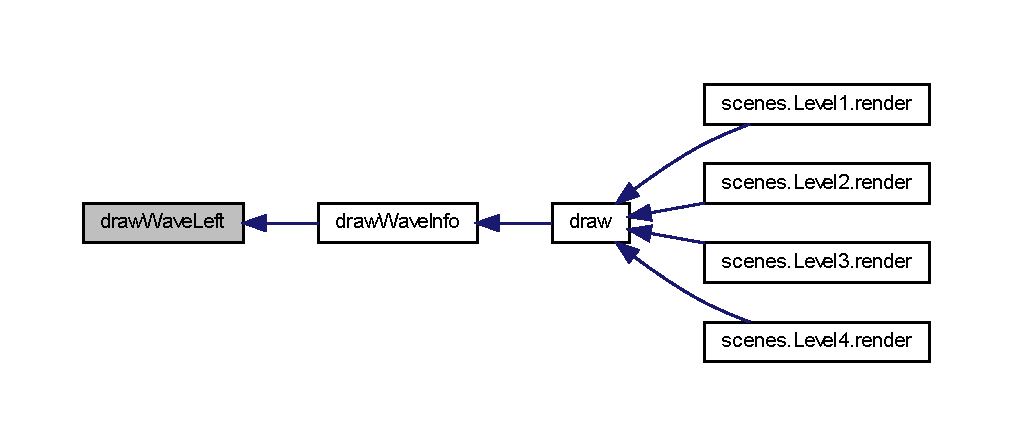
\includegraphics[width=350pt]{classui_1_1_action_bar_aeb491734ea2c8ae2f1be9db4f930d22a_icgraph}
\end{center}
\end{figure}
\mbox{\Hypertarget{classui_1_1_action_bar_a01f37d59ae4977fa55a1a6dd3e8bd543}\label{classui_1_1_action_bar_a01f37d59ae4977fa55a1a6dd3e8bd543}} 
\index{ui\+::\+Action\+Bar@{ui\+::\+Action\+Bar}!draw\+Wave\+Timer@{draw\+Wave\+Timer}}
\index{draw\+Wave\+Timer@{draw\+Wave\+Timer}!ui\+::\+Action\+Bar@{ui\+::\+Action\+Bar}}
\subsubsection{\texorpdfstring{draw\+Wave\+Timer()}{drawWaveTimer()}}
{\footnotesize\ttfamily void draw\+Wave\+Timer (\begin{DoxyParamCaption}\item[{Graphics}]{g }\end{DoxyParamCaption})\hspace{0.3cm}{\ttfamily [private]}}



disegna il timer dell\textquotesingle{}ondata. 


\begin{DoxyParams}{Parameters}
{\em g} & oggetto della grafica \\
\hline
\end{DoxyParams}


Definition at line 298 of file Action\+Bar.\+java.

Here is the call graph for this function\+:\nopagebreak
\begin{figure}[H]
\begin{center}
\leavevmode
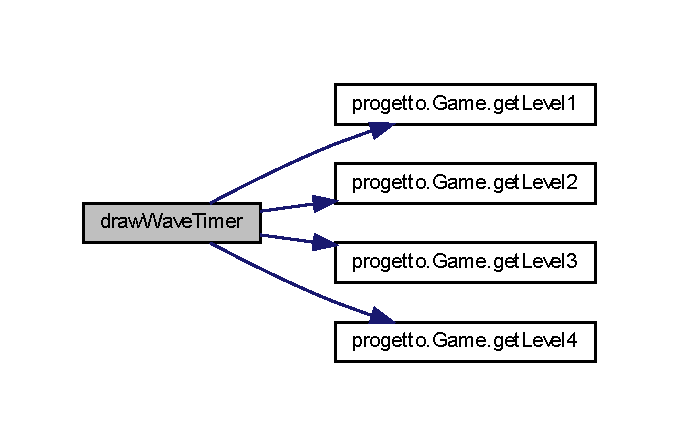
\includegraphics[width=326pt]{classui_1_1_action_bar_a01f37d59ae4977fa55a1a6dd3e8bd543_cgraph}
\end{center}
\end{figure}
Here is the caller graph for this function\+:\nopagebreak
\begin{figure}[H]
\begin{center}
\leavevmode
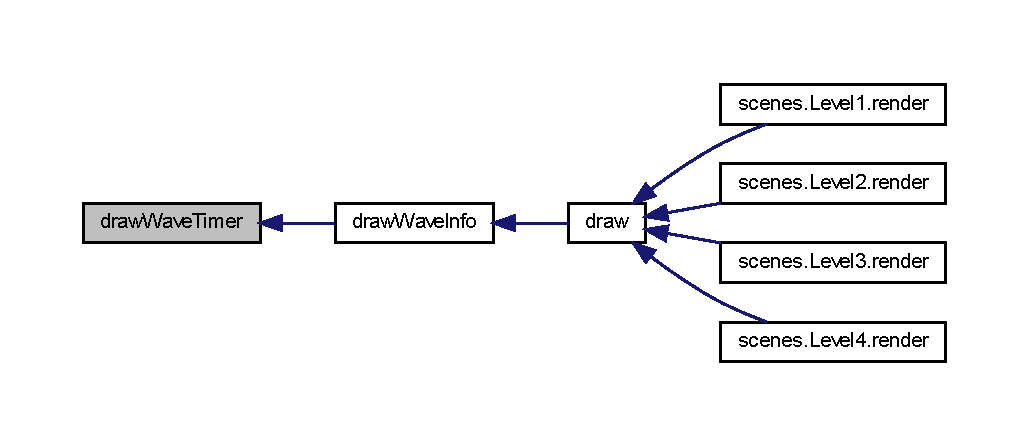
\includegraphics[width=350pt]{classui_1_1_action_bar_a01f37d59ae4977fa55a1a6dd3e8bd543_icgraph}
\end{center}
\end{figure}
\mbox{\Hypertarget{classui_1_1_action_bar_a6c5f59282a148a0d74bc5aa58d5ad307}\label{classui_1_1_action_bar_a6c5f59282a148a0d74bc5aa58d5ad307}} 
\index{ui\+::\+Action\+Bar@{ui\+::\+Action\+Bar}!get\+Level\+Up\+Cost@{get\+Level\+Up\+Cost}}
\index{get\+Level\+Up\+Cost@{get\+Level\+Up\+Cost}!ui\+::\+Action\+Bar@{ui\+::\+Action\+Bar}}
\subsubsection{\texorpdfstring{get\+Level\+Up\+Cost()}{getLevelUpCost()}}
{\footnotesize\ttfamily int get\+Level\+Up\+Cost (\begin{DoxyParamCaption}\item[{\hyperlink{classtowers_1_1_tower}{Tower}}]{displayed\+Tower }\end{DoxyParamCaption})}



restituisce il costo per upgradare la torre selezionata. 


\begin{DoxyParams}{Parameters}
{\em displayed\+Tower} & torre selezionata \\
\hline
\end{DoxyParams}


Definition at line 245 of file Action\+Bar.\+java.

Here is the call graph for this function\+:\nopagebreak
\begin{figure}[H]
\begin{center}
\leavevmode
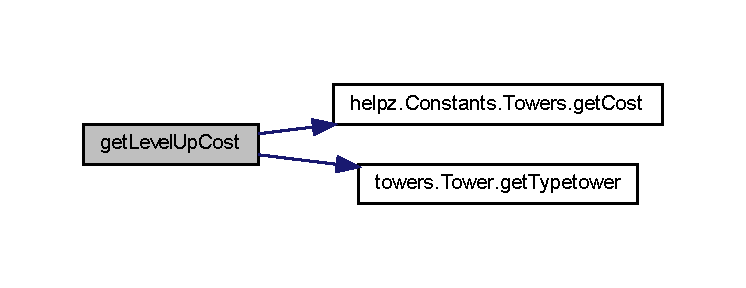
\includegraphics[width=350pt]{classui_1_1_action_bar_a6c5f59282a148a0d74bc5aa58d5ad307_cgraph}
\end{center}
\end{figure}
Here is the caller graph for this function\+:\nopagebreak
\begin{figure}[H]
\begin{center}
\leavevmode
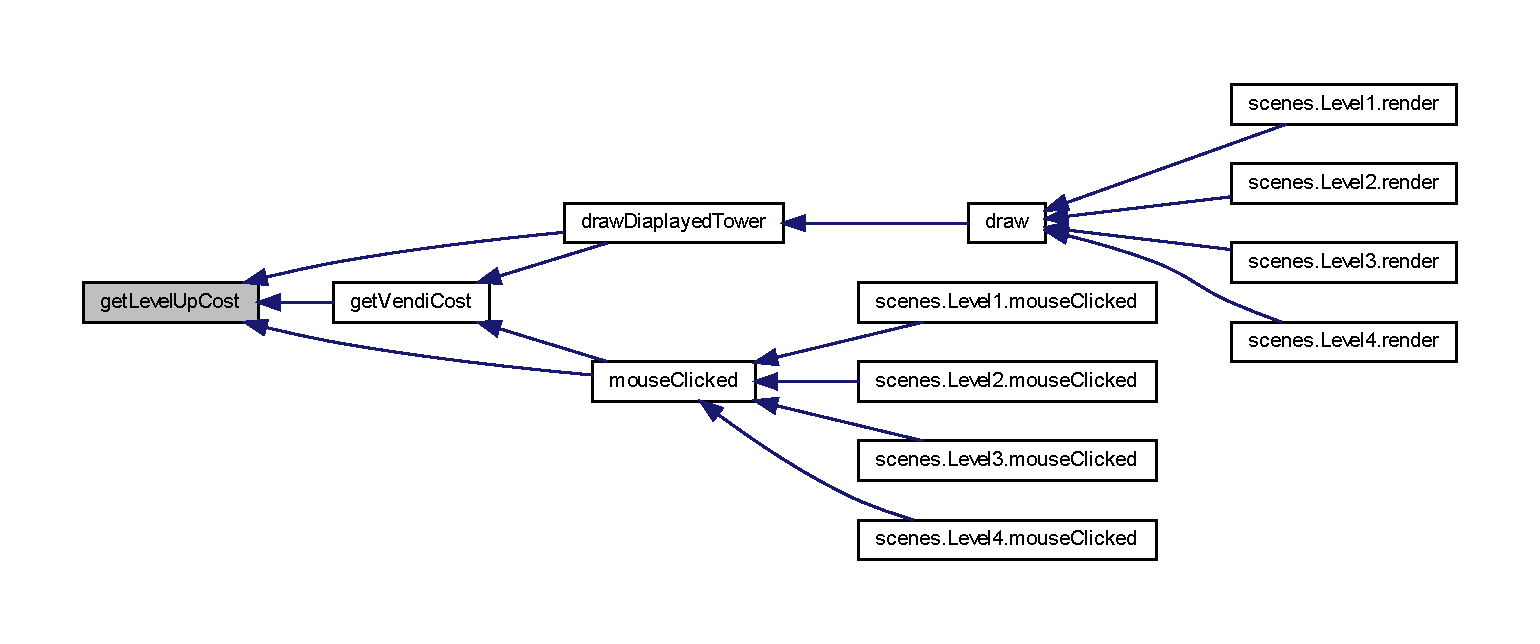
\includegraphics[width=350pt]{classui_1_1_action_bar_a6c5f59282a148a0d74bc5aa58d5ad307_icgraph}
\end{center}
\end{figure}
\mbox{\Hypertarget{classui_1_1_action_bar_aef810268cda93505da735c6c81136e00}\label{classui_1_1_action_bar_aef810268cda93505da735c6c81136e00}} 
\index{ui\+::\+Action\+Bar@{ui\+::\+Action\+Bar}!get\+Vendi\+Cost@{get\+Vendi\+Cost}}
\index{get\+Vendi\+Cost@{get\+Vendi\+Cost}!ui\+::\+Action\+Bar@{ui\+::\+Action\+Bar}}
\subsubsection{\texorpdfstring{get\+Vendi\+Cost()}{getVendiCost()}}
{\footnotesize\ttfamily int get\+Vendi\+Cost (\begin{DoxyParamCaption}\item[{\hyperlink{classtowers_1_1_tower}{Tower}}]{displayed\+Tower }\end{DoxyParamCaption})}



restituisce il guadagno della vendita della torre selezionata. 


\begin{DoxyParams}{Parameters}
{\em displayed\+Tower} & torre selezionata \\
\hline
\end{DoxyParams}


Definition at line 254 of file Action\+Bar.\+java.

Here is the call graph for this function\+:\nopagebreak
\begin{figure}[H]
\begin{center}
\leavevmode
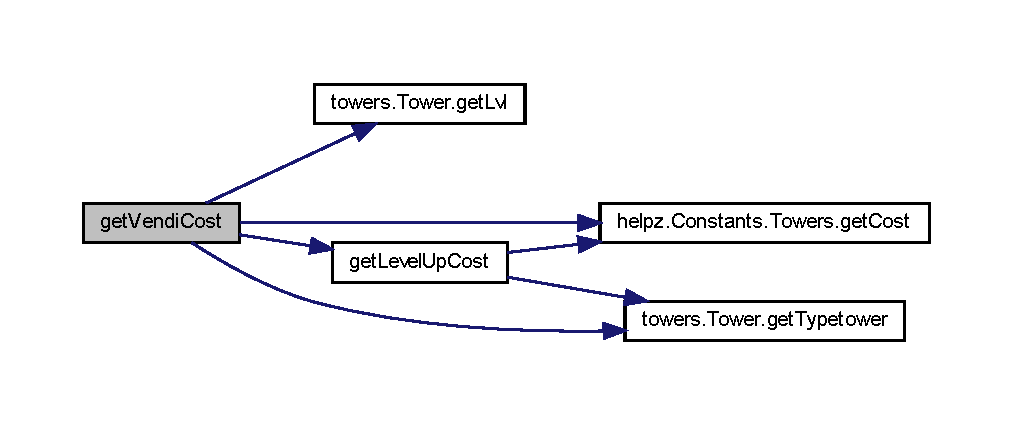
\includegraphics[width=350pt]{classui_1_1_action_bar_aef810268cda93505da735c6c81136e00_cgraph}
\end{center}
\end{figure}
Here is the caller graph for this function\+:\nopagebreak
\begin{figure}[H]
\begin{center}
\leavevmode
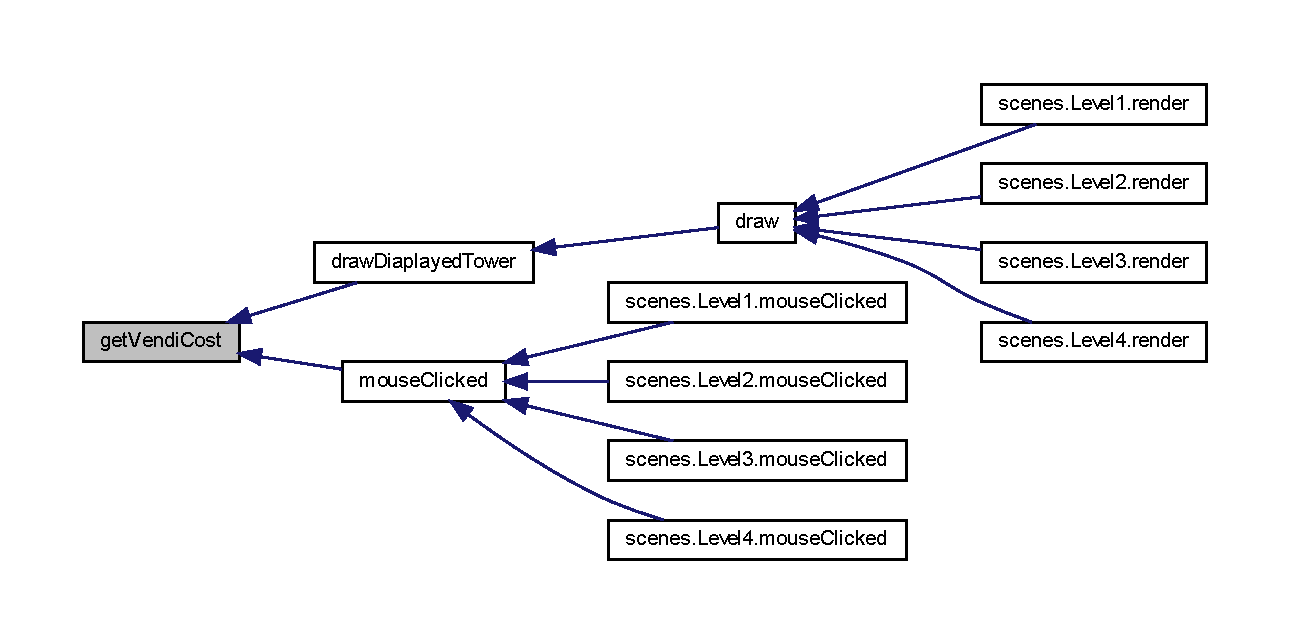
\includegraphics[width=350pt]{classui_1_1_action_bar_aef810268cda93505da735c6c81136e00_icgraph}
\end{center}
\end{figure}
\mbox{\Hypertarget{classui_1_1_action_bar_a3de978b9745ea5fdbe99d556e40166f6}\label{classui_1_1_action_bar_a3de978b9745ea5fdbe99d556e40166f6}} 
\index{ui\+::\+Action\+Bar@{ui\+::\+Action\+Bar}!get\+Vite@{get\+Vite}}
\index{get\+Vite@{get\+Vite}!ui\+::\+Action\+Bar@{ui\+::\+Action\+Bar}}
\subsubsection{\texorpdfstring{get\+Vite()}{getVite()}}
{\footnotesize\ttfamily int get\+Vite (\begin{DoxyParamCaption}{ }\end{DoxyParamCaption})}



restituisce il numero di vite. 

\begin{DoxyReturn}{Returns}
numero di vite 
\end{DoxyReturn}


Definition at line 488 of file Action\+Bar.\+java.

\mbox{\Hypertarget{classui_1_1_action_bar_aed9fe7e919d4355a7ad86701d44e1fea}\label{classui_1_1_action_bar_aed9fe7e919d4355a7ad86701d44e1fea}} 
\index{ui\+::\+Action\+Bar@{ui\+::\+Action\+Bar}!init\+Button@{init\+Button}}
\index{init\+Button@{init\+Button}!ui\+::\+Action\+Bar@{ui\+::\+Action\+Bar}}
\subsubsection{\texorpdfstring{init\+Button()}{initButton()}}
{\footnotesize\ttfamily void init\+Button (\begin{DoxyParamCaption}{ }\end{DoxyParamCaption})\hspace{0.3cm}{\ttfamily [private]}}



inizializza i bottoni. 



Definition at line 103 of file Action\+Bar.\+java.

Here is the call graph for this function\+:\nopagebreak
\begin{figure}[H]
\begin{center}
\leavevmode
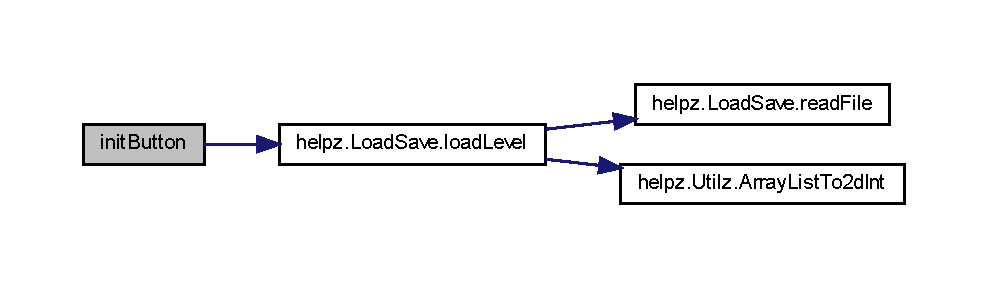
\includegraphics[width=350pt]{classui_1_1_action_bar_aed9fe7e919d4355a7ad86701d44e1fea_cgraph}
\end{center}
\end{figure}
Here is the caller graph for this function\+:\nopagebreak
\begin{figure}[H]
\begin{center}
\leavevmode
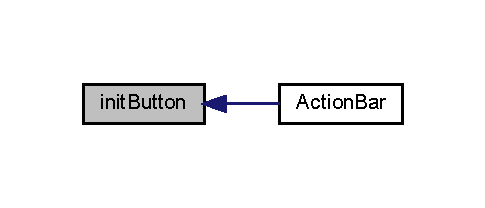
\includegraphics[width=233pt]{classui_1_1_action_bar_aed9fe7e919d4355a7ad86701d44e1fea_icgraph}
\end{center}
\end{figure}
\mbox{\Hypertarget{classui_1_1_action_bar_a45d56bd84238e8b56589dfc732e2b2cf}\label{classui_1_1_action_bar_a45d56bd84238e8b56589dfc732e2b2cf}} 
\index{ui\+::\+Action\+Bar@{ui\+::\+Action\+Bar}!mouse\+Clicked@{mouse\+Clicked}}
\index{mouse\+Clicked@{mouse\+Clicked}!ui\+::\+Action\+Bar@{ui\+::\+Action\+Bar}}
\subsubsection{\texorpdfstring{mouse\+Clicked()}{mouseClicked()}}
{\footnotesize\ttfamily void mouse\+Clicked (\begin{DoxyParamCaption}\item[{Mouse\+Event}]{e }\end{DoxyParamCaption})}



gestisce i click del mouse. 


\begin{DoxyParams}{Parameters}
{\em e} & evento del mouse \\
\hline
\end{DoxyParams}


Definition at line 522 of file Action\+Bar.\+java.

Here is the call graph for this function\+:\nopagebreak
\begin{figure}[H]
\begin{center}
\leavevmode
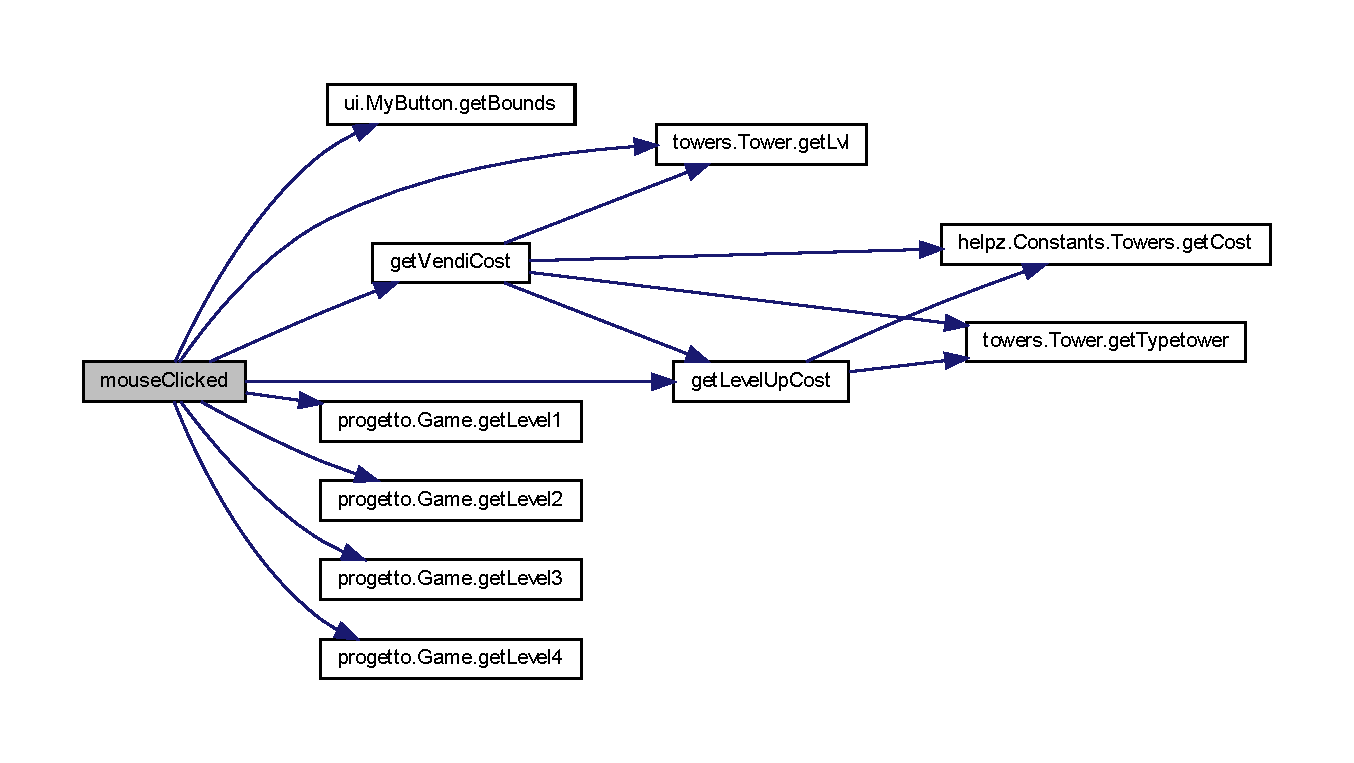
\includegraphics[width=350pt]{classui_1_1_action_bar_a45d56bd84238e8b56589dfc732e2b2cf_cgraph}
\end{center}
\end{figure}
Here is the caller graph for this function\+:\nopagebreak
\begin{figure}[H]
\begin{center}
\leavevmode
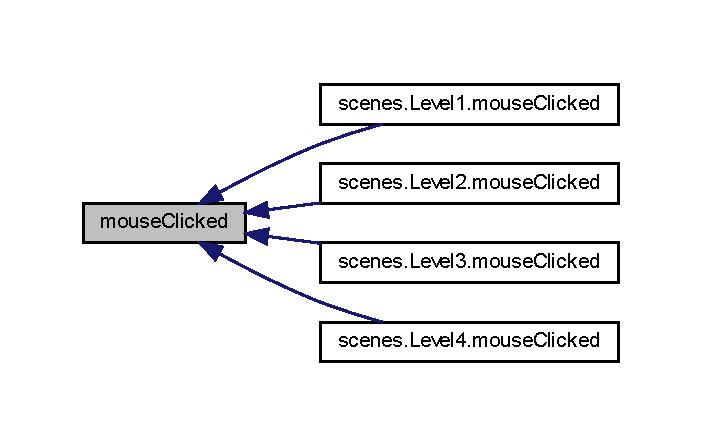
\includegraphics[width=337pt]{classui_1_1_action_bar_a45d56bd84238e8b56589dfc732e2b2cf_icgraph}
\end{center}
\end{figure}
\mbox{\Hypertarget{classui_1_1_action_bar_a2ca251710b65639ec80bc141edde60aa}\label{classui_1_1_action_bar_a2ca251710b65639ec80bc141edde60aa}} 
\index{ui\+::\+Action\+Bar@{ui\+::\+Action\+Bar}!mouse\+Moved@{mouse\+Moved}}
\index{mouse\+Moved@{mouse\+Moved}!ui\+::\+Action\+Bar@{ui\+::\+Action\+Bar}}
\subsubsection{\texorpdfstring{mouse\+Moved()}{mouseMoved()}}
{\footnotesize\ttfamily void mouse\+Moved (\begin{DoxyParamCaption}\item[{Mouse\+Event}]{e }\end{DoxyParamCaption})}



gestisce le move del mouse. 


\begin{DoxyParams}{Parameters}
{\em e} & evento del mouse \\
\hline
\end{DoxyParams}


Definition at line 577 of file Action\+Bar.\+java.

Here is the call graph for this function\+:\nopagebreak
\begin{figure}[H]
\begin{center}
\leavevmode
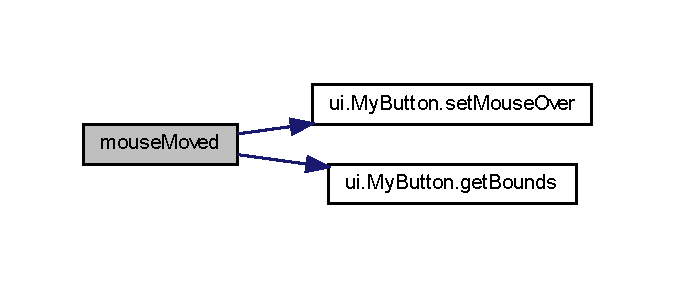
\includegraphics[width=324pt]{classui_1_1_action_bar_a2ca251710b65639ec80bc141edde60aa_cgraph}
\end{center}
\end{figure}
Here is the caller graph for this function\+:\nopagebreak
\begin{figure}[H]
\begin{center}
\leavevmode
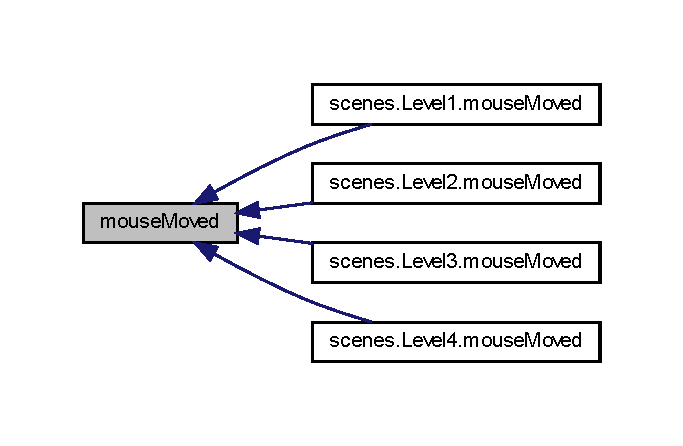
\includegraphics[width=328pt]{classui_1_1_action_bar_a2ca251710b65639ec80bc141edde60aa_icgraph}
\end{center}
\end{figure}
\mbox{\Hypertarget{classui_1_1_action_bar_aed82e1ce3dd3cf283d508c3ba3be70ef}\label{classui_1_1_action_bar_aed82e1ce3dd3cf283d508c3ba3be70ef}} 
\index{ui\+::\+Action\+Bar@{ui\+::\+Action\+Bar}!mouse\+Pressed@{mouse\+Pressed}}
\index{mouse\+Pressed@{mouse\+Pressed}!ui\+::\+Action\+Bar@{ui\+::\+Action\+Bar}}
\subsubsection{\texorpdfstring{mouse\+Pressed()}{mousePressed()}}
{\footnotesize\ttfamily void mouse\+Pressed (\begin{DoxyParamCaption}\item[{Mouse\+Event}]{e }\end{DoxyParamCaption})}



gestisce le press del mouse. 


\begin{DoxyParams}{Parameters}
{\em e} & evento del mouse \\
\hline
\end{DoxyParams}


Definition at line 622 of file Action\+Bar.\+java.

Here is the call graph for this function\+:\nopagebreak
\begin{figure}[H]
\begin{center}
\leavevmode
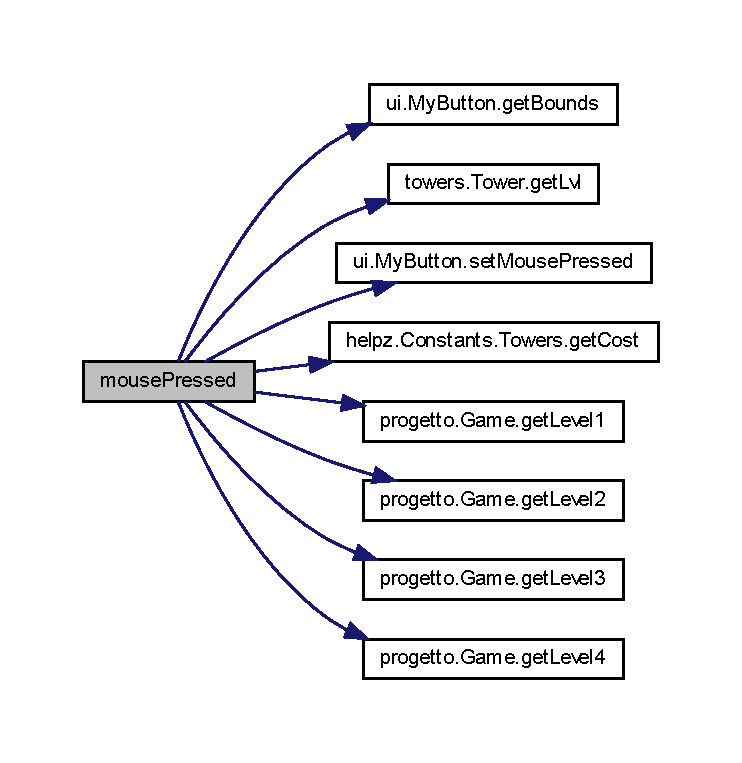
\includegraphics[width=350pt]{classui_1_1_action_bar_aed82e1ce3dd3cf283d508c3ba3be70ef_cgraph}
\end{center}
\end{figure}
Here is the caller graph for this function\+:\nopagebreak
\begin{figure}[H]
\begin{center}
\leavevmode
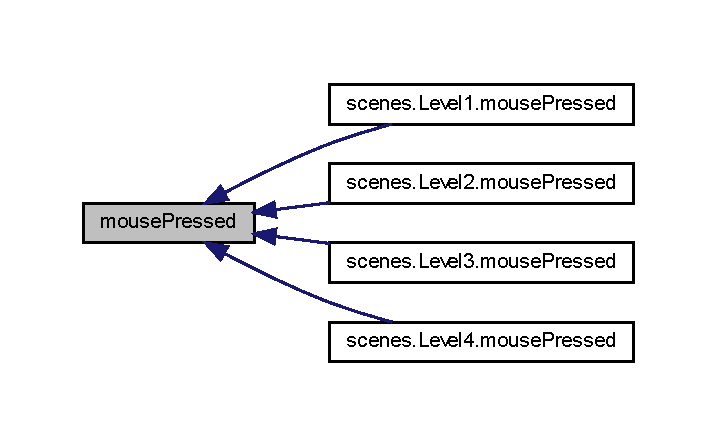
\includegraphics[width=344pt]{classui_1_1_action_bar_aed82e1ce3dd3cf283d508c3ba3be70ef_icgraph}
\end{center}
\end{figure}
\mbox{\Hypertarget{classui_1_1_action_bar_a87a07291794e15052db67f945d90853e}\label{classui_1_1_action_bar_a87a07291794e15052db67f945d90853e}} 
\index{ui\+::\+Action\+Bar@{ui\+::\+Action\+Bar}!mouse\+Released@{mouse\+Released}}
\index{mouse\+Released@{mouse\+Released}!ui\+::\+Action\+Bar@{ui\+::\+Action\+Bar}}
\subsubsection{\texorpdfstring{mouse\+Released()}{mouseReleased()}}
{\footnotesize\ttfamily void mouse\+Released (\begin{DoxyParamCaption}\item[{Mouse\+Event}]{e }\end{DoxyParamCaption})}



gestisce le release del mouse. 


\begin{DoxyParams}{Parameters}
{\em e} & evento del mouse \\
\hline
\end{DoxyParams}


Definition at line 676 of file Action\+Bar.\+java.

Here is the call graph for this function\+:\nopagebreak
\begin{figure}[H]
\begin{center}
\leavevmode
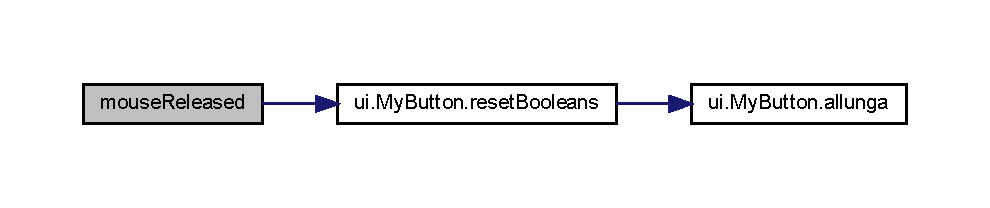
\includegraphics[width=350pt]{classui_1_1_action_bar_a87a07291794e15052db67f945d90853e_cgraph}
\end{center}
\end{figure}
Here is the caller graph for this function\+:\nopagebreak
\begin{figure}[H]
\begin{center}
\leavevmode
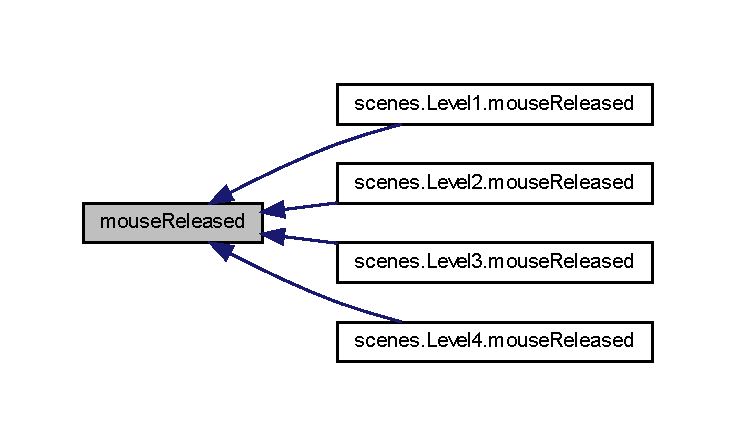
\includegraphics[width=350pt]{classui_1_1_action_bar_a87a07291794e15052db67f945d90853e_icgraph}
\end{center}
\end{figure}
\mbox{\Hypertarget{classui_1_1_action_bar_a99a8282ac7383f267261ca608cafe139}\label{classui_1_1_action_bar_a99a8282ac7383f267261ca608cafe139}} 
\index{ui\+::\+Action\+Bar@{ui\+::\+Action\+Bar}!remove\+Coin@{remove\+Coin}}
\index{remove\+Coin@{remove\+Coin}!ui\+::\+Action\+Bar@{ui\+::\+Action\+Bar}}
\subsubsection{\texorpdfstring{remove\+Coin()}{removeCoin()}}
{\footnotesize\ttfamily void remove\+Coin (\begin{DoxyParamCaption}\item[{int}]{type }\end{DoxyParamCaption})}



rimuove delle monete. 


\begin{DoxyParams}{Parameters}
{\em type} & tipo di acquisto \\
\hline
\end{DoxyParams}


Definition at line 437 of file Action\+Bar.\+java.

Here is the call graph for this function\+:\nopagebreak
\begin{figure}[H]
\begin{center}
\leavevmode
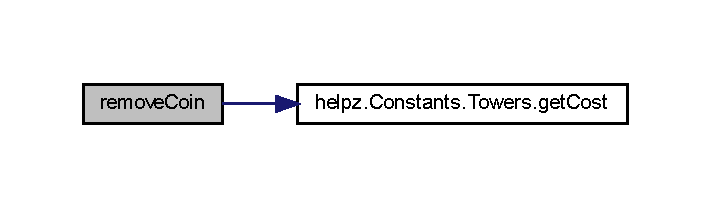
\includegraphics[width=341pt]{classui_1_1_action_bar_a99a8282ac7383f267261ca608cafe139_cgraph}
\end{center}
\end{figure}
Here is the caller graph for this function\+:\nopagebreak
\begin{figure}[H]
\begin{center}
\leavevmode
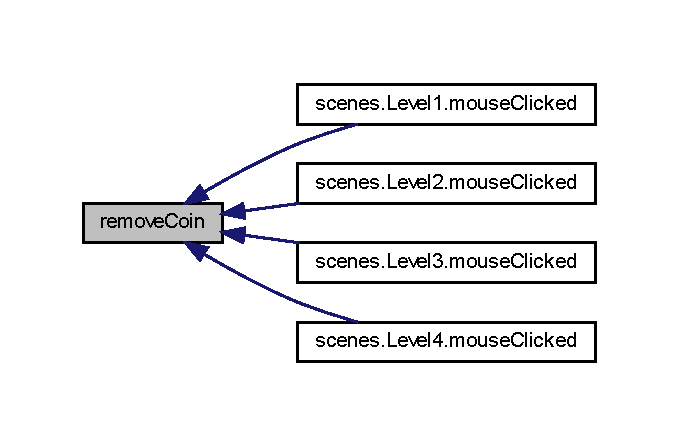
\includegraphics[width=326pt]{classui_1_1_action_bar_a99a8282ac7383f267261ca608cafe139_icgraph}
\end{center}
\end{figure}
\mbox{\Hypertarget{classui_1_1_action_bar_a484775c889ccd8602b66ad795b141534}\label{classui_1_1_action_bar_a484775c889ccd8602b66ad795b141534}} 
\index{ui\+::\+Action\+Bar@{ui\+::\+Action\+Bar}!rimuovi\+Vita@{rimuovi\+Vita}}
\index{rimuovi\+Vita@{rimuovi\+Vita}!ui\+::\+Action\+Bar@{ui\+::\+Action\+Bar}}
\subsubsection{\texorpdfstring{rimuovi\+Vita()}{rimuoviVita()}}
{\footnotesize\ttfamily void rimuovi\+Vita (\begin{DoxyParamCaption}{ }\end{DoxyParamCaption})}



rimuove una vita ed eventualmente termina il livello. 



Definition at line 496 of file Action\+Bar.\+java.

Here is the call graph for this function\+:\nopagebreak
\begin{figure}[H]
\begin{center}
\leavevmode
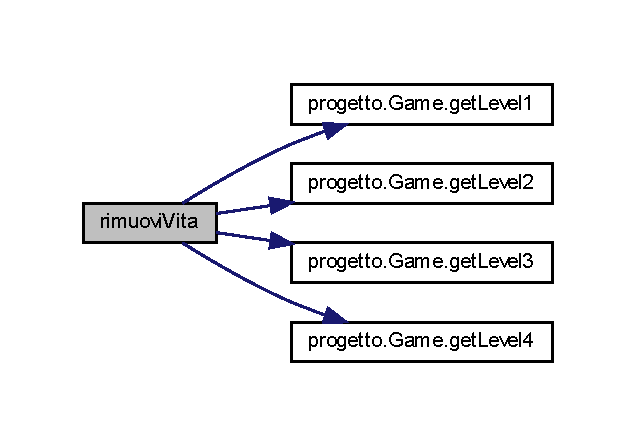
\includegraphics[width=305pt]{classui_1_1_action_bar_a484775c889ccd8602b66ad795b141534_cgraph}
\end{center}
\end{figure}
Here is the caller graph for this function\+:\nopagebreak
\begin{figure}[H]
\begin{center}
\leavevmode
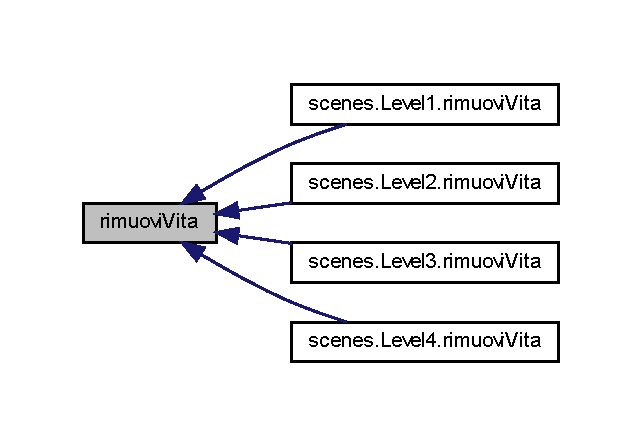
\includegraphics[width=308pt]{classui_1_1_action_bar_a484775c889ccd8602b66ad795b141534_icgraph}
\end{center}
\end{figure}


\subsection{Member Data Documentation}
\mbox{\Hypertarget{classui_1_1_action_bar_a02094092ae89aa4b23bff1976bcbf90d}\label{classui_1_1_action_bar_a02094092ae89aa4b23bff1976bcbf90d}} 
\index{ui\+::\+Action\+Bar@{ui\+::\+Action\+Bar}!c@{c}}
\index{c@{c}!ui\+::\+Action\+Bar@{ui\+::\+Action\+Bar}}
\subsubsection{\texorpdfstring{c}{c}}
{\footnotesize\ttfamily Color c\hspace{0.3cm}{\ttfamily [private]}}



Definition at line 38 of file Action\+Bar.\+java.

\mbox{\Hypertarget{classui_1_1_action_bar_a41de228368d6181324d7bfbdf40875e3}\label{classui_1_1_action_bar_a41de228368d6181324d7bfbdf40875e3}} 
\index{ui\+::\+Action\+Bar@{ui\+::\+Action\+Bar}!coin@{coin}}
\index{coin@{coin}!ui\+::\+Action\+Bar@{ui\+::\+Action\+Bar}}
\subsubsection{\texorpdfstring{coin}{coin}}
{\footnotesize\ttfamily int coin = 50\hspace{0.3cm}{\ttfamily [private]}}



Definition at line 56 of file Action\+Bar.\+java.

\mbox{\Hypertarget{classui_1_1_action_bar_a724d03f52f34297222dd1f423b96b6df}\label{classui_1_1_action_bar_a724d03f52f34297222dd1f423b96b6df}} 
\index{ui\+::\+Action\+Bar@{ui\+::\+Action\+Bar}!cuori@{cuori}}
\index{cuori@{cuori}!ui\+::\+Action\+Bar@{ui\+::\+Action\+Bar}}
\subsubsection{\texorpdfstring{cuori}{cuori}}
{\footnotesize\ttfamily Buffered\+Image \mbox{[}$\,$\mbox{]} cuori\hspace{0.3cm}{\ttfamily [private]}}



Definition at line 74 of file Action\+Bar.\+java.

\mbox{\Hypertarget{classui_1_1_action_bar_ab1f373e2f226eeef8843871210341966}\label{classui_1_1_action_bar_ab1f373e2f226eeef8843871210341966}} 
\index{ui\+::\+Action\+Bar@{ui\+::\+Action\+Bar}!decimal@{decimal}}
\index{decimal@{decimal}!ui\+::\+Action\+Bar@{ui\+::\+Action\+Bar}}
\subsubsection{\texorpdfstring{decimal}{decimal}}
{\footnotesize\ttfamily Decimal\+Format decimal = new Decimal\+Format(\char`\"{}0.\+0\char`\"{})\hspace{0.3cm}{\ttfamily [private]}}



Definition at line 291 of file Action\+Bar.\+java.

\mbox{\Hypertarget{classui_1_1_action_bar_a45f9b90370e0d7a88bd448d0c07267a4}\label{classui_1_1_action_bar_a45f9b90370e0d7a88bd448d0c07267a4}} 
\index{ui\+::\+Action\+Bar@{ui\+::\+Action\+Bar}!displayed\+Tower@{displayed\+Tower}}
\index{displayed\+Tower@{displayed\+Tower}!ui\+::\+Action\+Bar@{ui\+::\+Action\+Bar}}
\subsubsection{\texorpdfstring{displayed\+Tower}{displayedTower}}
{\footnotesize\ttfamily \hyperlink{classtowers_1_1_tower}{Tower} displayed\+Tower\hspace{0.3cm}{\ttfamily [private]}}



Definition at line 53 of file Action\+Bar.\+java.

\mbox{\Hypertarget{classui_1_1_action_bar_a3fb562f10e8f7f83cb2ed130eab6d439}\label{classui_1_1_action_bar_a3fb562f10e8f7f83cb2ed130eab6d439}} 
\index{ui\+::\+Action\+Bar@{ui\+::\+Action\+Bar}!f@{f}}
\index{f@{f}!ui\+::\+Action\+Bar@{ui\+::\+Action\+Bar}}
\subsubsection{\texorpdfstring{f}{f}}
{\footnotesize\ttfamily Font f\hspace{0.3cm}{\ttfamily [private]}}



Definition at line 35 of file Action\+Bar.\+java.

\mbox{\Hypertarget{classui_1_1_action_bar_ac6a5ed6191fcf3a5bf0445921feb4f48}\label{classui_1_1_action_bar_ac6a5ed6191fcf3a5bf0445921feb4f48}} 
\index{ui\+::\+Action\+Bar@{ui\+::\+Action\+Bar}!game@{game}}
\index{game@{game}!ui\+::\+Action\+Bar@{ui\+::\+Action\+Bar}}
\subsubsection{\texorpdfstring{game}{game}}
{\footnotesize\ttfamily \hyperlink{classprogetto_1_1_game}{Game} game\hspace{0.3cm}{\ttfamily [private]}}



Definition at line 41 of file Action\+Bar.\+java.

\mbox{\Hypertarget{classui_1_1_action_bar_af6b1162bc2f00f8d549aae075ddd5a8b}\label{classui_1_1_action_bar_af6b1162bc2f00f8d549aae075ddd5a8b}} 
\index{ui\+::\+Action\+Bar@{ui\+::\+Action\+Bar}!selected\+Tower@{selected\+Tower}}
\index{selected\+Tower@{selected\+Tower}!ui\+::\+Action\+Bar@{ui\+::\+Action\+Bar}}
\subsubsection{\texorpdfstring{selected\+Tower}{selectedTower}}
{\footnotesize\ttfamily \hyperlink{classtowers_1_1_tower}{Tower} selected\+Tower\hspace{0.3cm}{\ttfamily [private]}}



Definition at line 50 of file Action\+Bar.\+java.

\mbox{\Hypertarget{classui_1_1_action_bar_a520548d3a9dd584072883850aab5a593}\label{classui_1_1_action_bar_a520548d3a9dd584072883850aab5a593}} 
\index{ui\+::\+Action\+Bar@{ui\+::\+Action\+Bar}!showtowercost@{showtowercost}}
\index{showtowercost@{showtowercost}!ui\+::\+Action\+Bar@{ui\+::\+Action\+Bar}}
\subsubsection{\texorpdfstring{showtowercost}{showtowercost}}
{\footnotesize\ttfamily boolean showtowercost\hspace{0.3cm}{\ttfamily [private]}}



Definition at line 59 of file Action\+Bar.\+java.

\mbox{\Hypertarget{classui_1_1_action_bar_a91ac952876f776b3fbbc8519e093fdbf}\label{classui_1_1_action_bar_a91ac952876f776b3fbbc8519e093fdbf}} 
\index{ui\+::\+Action\+Bar@{ui\+::\+Action\+Bar}!state@{state}}
\index{state@{state}!ui\+::\+Action\+Bar@{ui\+::\+Action\+Bar}}
\subsubsection{\texorpdfstring{state}{state}}
{\footnotesize\ttfamily String state\hspace{0.3cm}{\ttfamily [private]}}



Definition at line 44 of file Action\+Bar.\+java.

\mbox{\Hypertarget{classui_1_1_action_bar_a6f80c6907b95d4fad643eb5cc2f9c343}\label{classui_1_1_action_bar_a6f80c6907b95d4fad643eb5cc2f9c343}} 
\index{ui\+::\+Action\+Bar@{ui\+::\+Action\+Bar}!tower\+Buttons@{tower\+Buttons}}
\index{tower\+Buttons@{tower\+Buttons}!ui\+::\+Action\+Bar@{ui\+::\+Action\+Bar}}
\subsubsection{\texorpdfstring{tower\+Buttons}{towerButtons}}
{\footnotesize\ttfamily \hyperlink{classui_1_1_my_button}{My\+Button} \mbox{[}$\,$\mbox{]} tower\+Buttons\hspace{0.3cm}{\ttfamily [private]}}



Definition at line 47 of file Action\+Bar.\+java.

\mbox{\Hypertarget{classui_1_1_action_bar_a62854c85f7998bd19028b0c197e96991}\label{classui_1_1_action_bar_a62854c85f7998bd19028b0c197e96991}} 
\index{ui\+::\+Action\+Bar@{ui\+::\+Action\+Bar}!towercost\+Type@{towercost\+Type}}
\index{towercost\+Type@{towercost\+Type}!ui\+::\+Action\+Bar@{ui\+::\+Action\+Bar}}
\subsubsection{\texorpdfstring{towercost\+Type}{towercostType}}
{\footnotesize\ttfamily int towercost\+Type\hspace{0.3cm}{\ttfamily [private]}}



Definition at line 62 of file Action\+Bar.\+java.

\mbox{\Hypertarget{classui_1_1_action_bar_ad424c422ef61739d7476cfafcb9aba28}\label{classui_1_1_action_bar_ad424c422ef61739d7476cfafcb9aba28}} 
\index{ui\+::\+Action\+Bar@{ui\+::\+Action\+Bar}!upgrade@{upgrade}}
\index{upgrade@{upgrade}!ui\+::\+Action\+Bar@{ui\+::\+Action\+Bar}}
\subsubsection{\texorpdfstring{upgrade}{upgrade}}
{\footnotesize\ttfamily \hyperlink{classui_1_1_my_button}{My\+Button} upgrade\hspace{0.3cm}{\ttfamily [private]}}



Definition at line 65 of file Action\+Bar.\+java.

\mbox{\Hypertarget{classui_1_1_action_bar_aca046bb433955f594a9af60ab1c34640}\label{classui_1_1_action_bar_aca046bb433955f594a9af60ab1c34640}} 
\index{ui\+::\+Action\+Bar@{ui\+::\+Action\+Bar}!vendi@{vendi}}
\index{vendi@{vendi}!ui\+::\+Action\+Bar@{ui\+::\+Action\+Bar}}
\subsubsection{\texorpdfstring{vendi}{vendi}}
{\footnotesize\ttfamily \hyperlink{classui_1_1_my_button}{My\+Button} vendi\hspace{0.3cm}{\ttfamily [private]}}



Definition at line 68 of file Action\+Bar.\+java.

\mbox{\Hypertarget{classui_1_1_action_bar_ace261aa2e09513de9acfbe08311c0f07}\label{classui_1_1_action_bar_ace261aa2e09513de9acfbe08311c0f07}} 
\index{ui\+::\+Action\+Bar@{ui\+::\+Action\+Bar}!vite@{vite}}
\index{vite@{vite}!ui\+::\+Action\+Bar@{ui\+::\+Action\+Bar}}
\subsubsection{\texorpdfstring{vite}{vite}}
{\footnotesize\ttfamily int vite = 3\hspace{0.3cm}{\ttfamily [private]}}



Definition at line 71 of file Action\+Bar.\+java.



The documentation for this class was generated from the following file\+:\begin{DoxyCompactItemize}
\item 
C\+:/\+Users/\+Utente/\+Documents/\+Git\+Hub/\+Plotty\+Towers/progetto/src/ui/\hyperlink{_action_bar_8java}{Action\+Bar.\+java}\end{DoxyCompactItemize}

\hypertarget{classtowers_1_1_attack_animation}{}\section{Attack\+Animation Class Reference}
\label{classtowers_1_1_attack_animation}\index{Attack\+Animation@{Attack\+Animation}}


gestisce le varie animazioni per ogni proiettile.  




Collaboration diagram for Attack\+Animation\+:\nopagebreak
\begin{figure}[H]
\begin{center}
\leavevmode
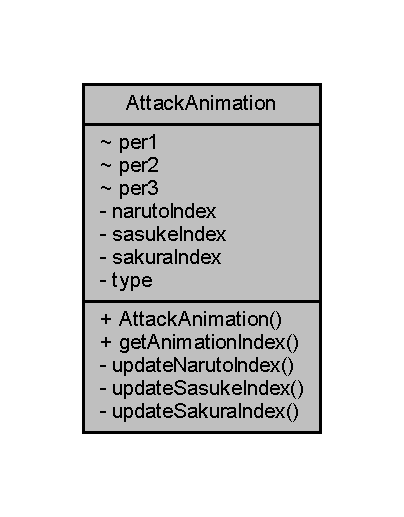
\includegraphics[width=194pt]{classtowers_1_1_attack_animation__coll__graph}
\end{center}
\end{figure}
\subsection*{Public Member Functions}
\begin{DoxyCompactItemize}
\item 
\hyperlink{classtowers_1_1_attack_animation_aa2f7222a5c2212052a4024e1f88e0f90}{Attack\+Animation} (int \hyperlink{classtowers_1_1_attack_animation_ac765329451135abec74c45e1897abf26}{type})
\begin{DoxyCompactList}\small\item\em costruttore setta il tipo di proiettile \end{DoxyCompactList}\item 
int \hyperlink{classtowers_1_1_attack_animation_ae8c4fe920791c4525eb1a9ab79d1e3b7}{get\+Animation\+Index} ()
\begin{DoxyCompactList}\small\item\em ritorna l\textquotesingle{}indice dell\textquotesingle{}animazione del type corrente. \end{DoxyCompactList}\end{DoxyCompactItemize}
\subsection*{Private Member Functions}
\begin{DoxyCompactItemize}
\item 
int \hyperlink{classtowers_1_1_attack_animation_a9a43224ece8c2b408bea79a17a40926a}{update\+Naruto\+Index} ()
\begin{DoxyCompactList}\small\item\em aggiorna e ritorna l\textquotesingle{}indice dell\textquotesingle{}animazione di naruto. \end{DoxyCompactList}\item 
int \hyperlink{classtowers_1_1_attack_animation_a6b8b22718154d24a23128663058f8780}{update\+Sasuke\+Index} ()
\begin{DoxyCompactList}\small\item\em aggiorna e ritorna l\textquotesingle{}indice dell\textquotesingle{}animazione di sasuke. \end{DoxyCompactList}\item 
int \hyperlink{classtowers_1_1_attack_animation_a1f8c2a2ac98f9746a0175442814aca4b}{update\+Sakura\+Index} ()
\begin{DoxyCompactList}\small\item\em aggiorna e ritorna l\textquotesingle{}indice dell\textquotesingle{}animazione di sakura. \end{DoxyCompactList}\end{DoxyCompactItemize}
\subsection*{Private Attributes}
\begin{DoxyCompactItemize}
\item 
int \hyperlink{classtowers_1_1_attack_animation_a0d5d70f714c6c696174fc8b20caab8de}{naruto\+Index} =0
\item 
int \hyperlink{classtowers_1_1_attack_animation_a607a6f73da61681d9d1d693943346acf}{sasuke\+Index} =0
\item 
int \hyperlink{classtowers_1_1_attack_animation_a9717cb2cb5245abda5bdc9c80b1eb416}{sakura\+Index} =0
\item 
int \hyperlink{classtowers_1_1_attack_animation_ac765329451135abec74c45e1897abf26}{type}
\end{DoxyCompactItemize}


\subsection{Detailed Description}
gestisce le varie animazioni per ogni proiettile. 

Definition at line 20 of file Attack\+Animation.\+java.



\subsection{Constructor \& Destructor Documentation}
\mbox{\Hypertarget{classtowers_1_1_attack_animation_aa2f7222a5c2212052a4024e1f88e0f90}\label{classtowers_1_1_attack_animation_aa2f7222a5c2212052a4024e1f88e0f90}} 
\index{towers\+::\+Attack\+Animation@{towers\+::\+Attack\+Animation}!Attack\+Animation@{Attack\+Animation}}
\index{Attack\+Animation@{Attack\+Animation}!towers\+::\+Attack\+Animation@{towers\+::\+Attack\+Animation}}
\subsubsection{\texorpdfstring{Attack\+Animation()}{AttackAnimation()}}
{\footnotesize\ttfamily \hyperlink{classtowers_1_1_attack_animation}{Attack\+Animation} (\begin{DoxyParamCaption}\item[{int}]{type }\end{DoxyParamCaption})}



costruttore setta il tipo di proiettile 


\begin{DoxyParams}{Parameters}
{\em type} & proiettile \\
\hline
\end{DoxyParams}


Definition at line 39 of file Attack\+Animation.\+java.



\subsection{Member Function Documentation}
\mbox{\Hypertarget{classtowers_1_1_attack_animation_ae8c4fe920791c4525eb1a9ab79d1e3b7}\label{classtowers_1_1_attack_animation_ae8c4fe920791c4525eb1a9ab79d1e3b7}} 
\index{towers\+::\+Attack\+Animation@{towers\+::\+Attack\+Animation}!get\+Animation\+Index@{get\+Animation\+Index}}
\index{get\+Animation\+Index@{get\+Animation\+Index}!towers\+::\+Attack\+Animation@{towers\+::\+Attack\+Animation}}
\subsubsection{\texorpdfstring{get\+Animation\+Index()}{getAnimationIndex()}}
{\footnotesize\ttfamily int get\+Animation\+Index (\begin{DoxyParamCaption}{ }\end{DoxyParamCaption})}



ritorna l\textquotesingle{}indice dell\textquotesingle{}animazione del type corrente. 

\begin{DoxyReturn}{Returns}
indice dell\textquotesingle{}animazione 
\end{DoxyReturn}


Definition at line 48 of file Attack\+Animation.\+java.

Here is the call graph for this function\+:\nopagebreak
\begin{figure}[H]
\begin{center}
\leavevmode
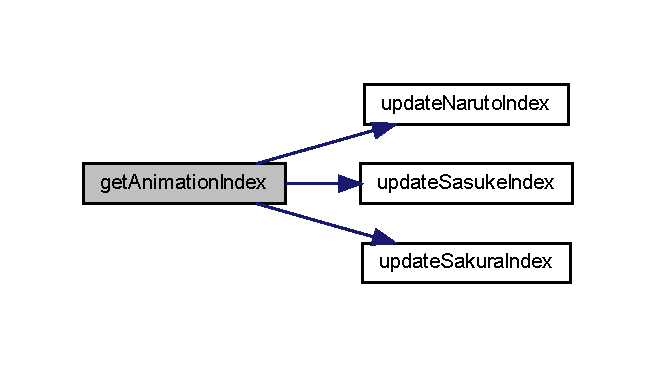
\includegraphics[width=315pt]{classtowers_1_1_attack_animation_ae8c4fe920791c4525eb1a9ab79d1e3b7_cgraph}
\end{center}
\end{figure}
Here is the caller graph for this function\+:\nopagebreak
\begin{figure}[H]
\begin{center}
\leavevmode
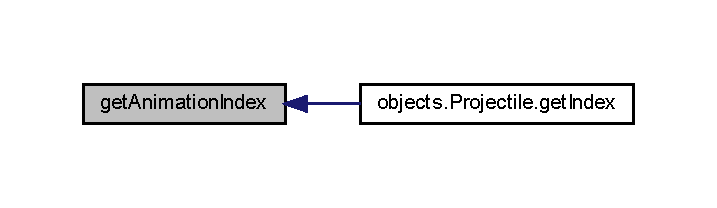
\includegraphics[width=344pt]{classtowers_1_1_attack_animation_ae8c4fe920791c4525eb1a9ab79d1e3b7_icgraph}
\end{center}
\end{figure}
\mbox{\Hypertarget{classtowers_1_1_attack_animation_a9a43224ece8c2b408bea79a17a40926a}\label{classtowers_1_1_attack_animation_a9a43224ece8c2b408bea79a17a40926a}} 
\index{towers\+::\+Attack\+Animation@{towers\+::\+Attack\+Animation}!update\+Naruto\+Index@{update\+Naruto\+Index}}
\index{update\+Naruto\+Index@{update\+Naruto\+Index}!towers\+::\+Attack\+Animation@{towers\+::\+Attack\+Animation}}
\subsubsection{\texorpdfstring{update\+Naruto\+Index()}{updateNarutoIndex()}}
{\footnotesize\ttfamily int update\+Naruto\+Index (\begin{DoxyParamCaption}{ }\end{DoxyParamCaption})\hspace{0.3cm}{\ttfamily [private]}}



aggiorna e ritorna l\textquotesingle{}indice dell\textquotesingle{}animazione di naruto. 

\begin{DoxyReturn}{Returns}
index dell\textquotesingle{}animazione 
\end{DoxyReturn}


Definition at line 70 of file Attack\+Animation.\+java.

Here is the caller graph for this function\+:\nopagebreak
\begin{figure}[H]
\begin{center}
\leavevmode
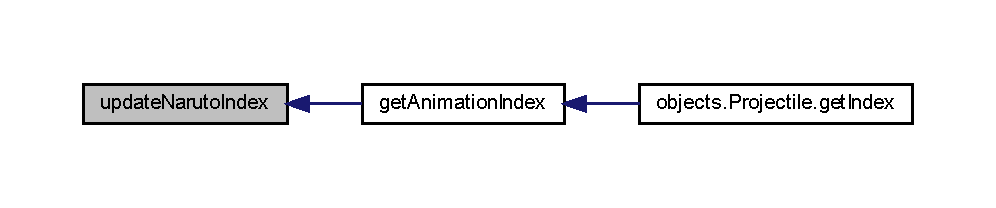
\includegraphics[width=350pt]{classtowers_1_1_attack_animation_a9a43224ece8c2b408bea79a17a40926a_icgraph}
\end{center}
\end{figure}
\mbox{\Hypertarget{classtowers_1_1_attack_animation_a1f8c2a2ac98f9746a0175442814aca4b}\label{classtowers_1_1_attack_animation_a1f8c2a2ac98f9746a0175442814aca4b}} 
\index{towers\+::\+Attack\+Animation@{towers\+::\+Attack\+Animation}!update\+Sakura\+Index@{update\+Sakura\+Index}}
\index{update\+Sakura\+Index@{update\+Sakura\+Index}!towers\+::\+Attack\+Animation@{towers\+::\+Attack\+Animation}}
\subsubsection{\texorpdfstring{update\+Sakura\+Index()}{updateSakuraIndex()}}
{\footnotesize\ttfamily int update\+Sakura\+Index (\begin{DoxyParamCaption}{ }\end{DoxyParamCaption})\hspace{0.3cm}{\ttfamily [private]}}



aggiorna e ritorna l\textquotesingle{}indice dell\textquotesingle{}animazione di sakura. 

\begin{DoxyReturn}{Returns}
index dell\textquotesingle{}animazione 
\end{DoxyReturn}


Definition at line 108 of file Attack\+Animation.\+java.

Here is the caller graph for this function\+:\nopagebreak
\begin{figure}[H]
\begin{center}
\leavevmode
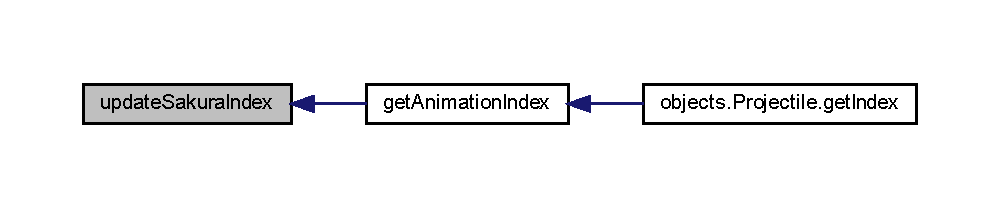
\includegraphics[width=350pt]{classtowers_1_1_attack_animation_a1f8c2a2ac98f9746a0175442814aca4b_icgraph}
\end{center}
\end{figure}
\mbox{\Hypertarget{classtowers_1_1_attack_animation_a6b8b22718154d24a23128663058f8780}\label{classtowers_1_1_attack_animation_a6b8b22718154d24a23128663058f8780}} 
\index{towers\+::\+Attack\+Animation@{towers\+::\+Attack\+Animation}!update\+Sasuke\+Index@{update\+Sasuke\+Index}}
\index{update\+Sasuke\+Index@{update\+Sasuke\+Index}!towers\+::\+Attack\+Animation@{towers\+::\+Attack\+Animation}}
\subsubsection{\texorpdfstring{update\+Sasuke\+Index()}{updateSasukeIndex()}}
{\footnotesize\ttfamily int update\+Sasuke\+Index (\begin{DoxyParamCaption}{ }\end{DoxyParamCaption})\hspace{0.3cm}{\ttfamily [private]}}



aggiorna e ritorna l\textquotesingle{}indice dell\textquotesingle{}animazione di sasuke. 

\begin{DoxyReturn}{Returns}
index dell\textquotesingle{}animazione 
\end{DoxyReturn}


Definition at line 89 of file Attack\+Animation.\+java.

Here is the caller graph for this function\+:\nopagebreak
\begin{figure}[H]
\begin{center}
\leavevmode
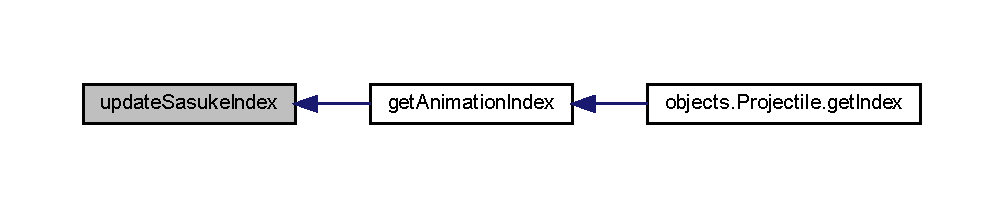
\includegraphics[width=350pt]{classtowers_1_1_attack_animation_a6b8b22718154d24a23128663058f8780_icgraph}
\end{center}
\end{figure}


\subsection{Member Data Documentation}
\mbox{\Hypertarget{classtowers_1_1_attack_animation_a0d5d70f714c6c696174fc8b20caab8de}\label{classtowers_1_1_attack_animation_a0d5d70f714c6c696174fc8b20caab8de}} 
\index{towers\+::\+Attack\+Animation@{towers\+::\+Attack\+Animation}!naruto\+Index@{naruto\+Index}}
\index{naruto\+Index@{naruto\+Index}!towers\+::\+Attack\+Animation@{towers\+::\+Attack\+Animation}}
\subsubsection{\texorpdfstring{naruto\+Index}{narutoIndex}}
{\footnotesize\ttfamily int naruto\+Index =0\hspace{0.3cm}{\ttfamily [private]}}



Definition at line 23 of file Attack\+Animation.\+java.

\mbox{\Hypertarget{classtowers_1_1_attack_animation_a9717cb2cb5245abda5bdc9c80b1eb416}\label{classtowers_1_1_attack_animation_a9717cb2cb5245abda5bdc9c80b1eb416}} 
\index{towers\+::\+Attack\+Animation@{towers\+::\+Attack\+Animation}!sakura\+Index@{sakura\+Index}}
\index{sakura\+Index@{sakura\+Index}!towers\+::\+Attack\+Animation@{towers\+::\+Attack\+Animation}}
\subsubsection{\texorpdfstring{sakura\+Index}{sakuraIndex}}
{\footnotesize\ttfamily int sakura\+Index =0\hspace{0.3cm}{\ttfamily [private]}}



Definition at line 29 of file Attack\+Animation.\+java.

\mbox{\Hypertarget{classtowers_1_1_attack_animation_a607a6f73da61681d9d1d693943346acf}\label{classtowers_1_1_attack_animation_a607a6f73da61681d9d1d693943346acf}} 
\index{towers\+::\+Attack\+Animation@{towers\+::\+Attack\+Animation}!sasuke\+Index@{sasuke\+Index}}
\index{sasuke\+Index@{sasuke\+Index}!towers\+::\+Attack\+Animation@{towers\+::\+Attack\+Animation}}
\subsubsection{\texorpdfstring{sasuke\+Index}{sasukeIndex}}
{\footnotesize\ttfamily int sasuke\+Index =0\hspace{0.3cm}{\ttfamily [private]}}



Definition at line 26 of file Attack\+Animation.\+java.

\mbox{\Hypertarget{classtowers_1_1_attack_animation_ac765329451135abec74c45e1897abf26}\label{classtowers_1_1_attack_animation_ac765329451135abec74c45e1897abf26}} 
\index{towers\+::\+Attack\+Animation@{towers\+::\+Attack\+Animation}!type@{type}}
\index{type@{type}!towers\+::\+Attack\+Animation@{towers\+::\+Attack\+Animation}}
\subsubsection{\texorpdfstring{type}{type}}
{\footnotesize\ttfamily int type\hspace{0.3cm}{\ttfamily [private]}}



Definition at line 32 of file Attack\+Animation.\+java.



The documentation for this class was generated from the following file\+:\begin{DoxyCompactItemize}
\item 
C\+:/\+Users/\+Utente/\+Documents/\+Git\+Hub/\+Plotty\+Towers/progetto/src/towers/\hyperlink{_attack_animation_8java}{Attack\+Animation.\+java}\end{DoxyCompactItemize}

\hypertarget{classui_1_1_bar}{}\section{Bar Class Reference}
\label{classui_1_1_bar}\index{Bar@{Bar}}


classe padre delle altre barre  




Inheritance diagram for Bar\+:\nopagebreak
\begin{figure}[H]
\begin{center}
\leavevmode
\includegraphics[height=550pt]{classui_1_1_bar__inherit__graph}
\end{center}
\end{figure}


Collaboration diagram for Bar\+:\nopagebreak
\begin{figure}[H]
\begin{center}
\leavevmode
\includegraphics[width=131pt]{classui_1_1_bar__coll__graph}
\end{center}
\end{figure}
\subsection*{Public Member Functions}
\begin{DoxyCompactItemize}
\item 
\hyperlink{classui_1_1_bar_a9048e88559d1d799814949815b2ab2d9}{Bar} (int \hyperlink{classui_1_1_bar_a6150e0515f7202e2fb518f7206ed97dc}{x}, int \hyperlink{classui_1_1_bar_a0a2f84ed7838f07779ae24c5a9086d33}{y}, int \hyperlink{classui_1_1_bar_a2474a5474cbff19523a51eb1de01cda4}{width}, int \hyperlink{classui_1_1_bar_ad12fc34ce789bce6c8a05d8a17138534}{height})
\begin{DoxyCompactList}\small\item\em costruttore inizializza tutte le variabili. \end{DoxyCompactList}\end{DoxyCompactItemize}
\subsection*{Protected Attributes}
\begin{DoxyCompactItemize}
\item 
int \hyperlink{classui_1_1_bar_a6150e0515f7202e2fb518f7206ed97dc}{x}
\item 
int \hyperlink{classui_1_1_bar_a0a2f84ed7838f07779ae24c5a9086d33}{y}
\item 
int \hyperlink{classui_1_1_bar_a2474a5474cbff19523a51eb1de01cda4}{width}
\item 
int \hyperlink{classui_1_1_bar_ad12fc34ce789bce6c8a05d8a17138534}{height}
\end{DoxyCompactItemize}


\subsection{Detailed Description}
classe padre delle altre barre 

Definition at line 20 of file Bar.\+java.



\subsection{Constructor \& Destructor Documentation}
\mbox{\Hypertarget{classui_1_1_bar_a9048e88559d1d799814949815b2ab2d9}\label{classui_1_1_bar_a9048e88559d1d799814949815b2ab2d9}} 
\index{ui\+::\+Bar@{ui\+::\+Bar}!Bar@{Bar}}
\index{Bar@{Bar}!ui\+::\+Bar@{ui\+::\+Bar}}
\subsubsection{\texorpdfstring{Bar()}{Bar()}}
{\footnotesize\ttfamily \hyperlink{classui_1_1_bar}{Bar} (\begin{DoxyParamCaption}\item[{int}]{x,  }\item[{int}]{y,  }\item[{int}]{width,  }\item[{int}]{height }\end{DoxyParamCaption})}



costruttore inizializza tutte le variabili. 


\begin{DoxyParams}{Parameters}
{\em x} & coordinata \\
\hline
{\em y} & coordinata \\
\hline
{\em width} & larghezza \\
\hline
{\em height} & altezza \\
\hline
\end{DoxyParams}


Definition at line 42 of file Bar.\+java.



\subsection{Member Data Documentation}
\mbox{\Hypertarget{classui_1_1_bar_ad12fc34ce789bce6c8a05d8a17138534}\label{classui_1_1_bar_ad12fc34ce789bce6c8a05d8a17138534}} 
\index{ui\+::\+Bar@{ui\+::\+Bar}!height@{height}}
\index{height@{height}!ui\+::\+Bar@{ui\+::\+Bar}}
\subsubsection{\texorpdfstring{height}{height}}
{\footnotesize\ttfamily int height\hspace{0.3cm}{\ttfamily [protected]}}



Definition at line 32 of file Bar.\+java.

\mbox{\Hypertarget{classui_1_1_bar_a2474a5474cbff19523a51eb1de01cda4}\label{classui_1_1_bar_a2474a5474cbff19523a51eb1de01cda4}} 
\index{ui\+::\+Bar@{ui\+::\+Bar}!width@{width}}
\index{width@{width}!ui\+::\+Bar@{ui\+::\+Bar}}
\subsubsection{\texorpdfstring{width}{width}}
{\footnotesize\ttfamily int width\hspace{0.3cm}{\ttfamily [protected]}}



Definition at line 29 of file Bar.\+java.

\mbox{\Hypertarget{classui_1_1_bar_a6150e0515f7202e2fb518f7206ed97dc}\label{classui_1_1_bar_a6150e0515f7202e2fb518f7206ed97dc}} 
\index{ui\+::\+Bar@{ui\+::\+Bar}!x@{x}}
\index{x@{x}!ui\+::\+Bar@{ui\+::\+Bar}}
\subsubsection{\texorpdfstring{x}{x}}
{\footnotesize\ttfamily int x\hspace{0.3cm}{\ttfamily [protected]}}



Definition at line 23 of file Bar.\+java.

\mbox{\Hypertarget{classui_1_1_bar_a0a2f84ed7838f07779ae24c5a9086d33}\label{classui_1_1_bar_a0a2f84ed7838f07779ae24c5a9086d33}} 
\index{ui\+::\+Bar@{ui\+::\+Bar}!y@{y}}
\index{y@{y}!ui\+::\+Bar@{ui\+::\+Bar}}
\subsubsection{\texorpdfstring{y}{y}}
{\footnotesize\ttfamily int y\hspace{0.3cm}{\ttfamily [protected]}}



Definition at line 26 of file Bar.\+java.



The documentation for this class was generated from the following file\+:\begin{DoxyCompactItemize}
\item 
C\+:/\+Users/\+Utente/\+Documents/\+Git\+Hub/\+Plotty\+Towers/progetto/src/ui/\hyperlink{_bar_8java}{Bar.\+java}\end{DoxyCompactItemize}

\hypertarget{classhelpz_1_1_constants}{}\section{Constants Class Reference}
\label{classhelpz_1_1_constants}\index{Constants@{Constants}}


gestisce le costanti  




Collaboration diagram for Constants\+:\nopagebreak
\begin{figure}[H]
\begin{center}
\leavevmode
\includegraphics[width=141pt]{classhelpz_1_1_constants__coll__graph}
\end{center}
\end{figure}
\subsection*{Classes}
\begin{DoxyCompactItemize}
\item 
class \hyperlink{classhelpz_1_1_constants_1_1_direction}{Direction}
\item 
class \hyperlink{classhelpz_1_1_constants_1_1_enemy}{Enemy}
\item 
class \hyperlink{classhelpz_1_1_constants_1_1_projectiles}{Projectiles}
\item 
class \hyperlink{classhelpz_1_1_constants_1_1_tiles}{Tiles}
\item 
class \hyperlink{classhelpz_1_1_constants_1_1_towers}{Towers}
\end{DoxyCompactItemize}


\subsection{Detailed Description}
gestisce le costanti 

Definition at line 18 of file Constants.\+java.



The documentation for this class was generated from the following file\+:\begin{DoxyCompactItemize}
\item 
C\+:/\+Users/\+Utente/\+Documents/\+Git\+Hub/\+Plotty\+Towers/progetto/src/helpz/\hyperlink{_constants_8java}{Constants.\+java}\end{DoxyCompactItemize}

\hypertarget{classhelpz_1_1_constants_1_1_direction}{}\section{Constants.\+Direction Class Reference}
\label{classhelpz_1_1_constants_1_1_direction}\index{Constants.\+Direction@{Constants.\+Direction}}


Collaboration diagram for Constants.\+Direction\+:\nopagebreak
\begin{figure}[H]
\begin{center}
\leavevmode
\includegraphics[width=182pt]{classhelpz_1_1_constants_1_1_direction__coll__graph}
\end{center}
\end{figure}
\subsection*{Static Public Attributes}
\begin{DoxyCompactItemize}
\item 
static final int \hyperlink{classhelpz_1_1_constants_1_1_direction_a8f5895cd15bc59e07a2c1e4d55449333}{L\+E\+FT} = 0
\item 
static final int \hyperlink{classhelpz_1_1_constants_1_1_direction_ad6535a3a47426014d15edf19175a7293}{UP} = 1
\item 
static final int \hyperlink{classhelpz_1_1_constants_1_1_direction_ae432a3ecfa87c4a57b4143a165ddd72e}{R\+I\+G\+HT} = 2
\item 
static final int \hyperlink{classhelpz_1_1_constants_1_1_direction_aa9a430bba08262217c6e4f8613fedd9e}{D\+O\+WN} = 3
\end{DoxyCompactItemize}


\subsection{Detailed Description}


Definition at line 20 of file Constants.\+java.



\subsection{Member Data Documentation}
\mbox{\Hypertarget{classhelpz_1_1_constants_1_1_direction_aa9a430bba08262217c6e4f8613fedd9e}\label{classhelpz_1_1_constants_1_1_direction_aa9a430bba08262217c6e4f8613fedd9e}} 
\index{helpz\+::\+Constants\+::\+Direction@{helpz\+::\+Constants\+::\+Direction}!D\+O\+WN@{D\+O\+WN}}
\index{D\+O\+WN@{D\+O\+WN}!helpz\+::\+Constants\+::\+Direction@{helpz\+::\+Constants\+::\+Direction}}
\subsubsection{\texorpdfstring{D\+O\+WN}{DOWN}}
{\footnotesize\ttfamily final int D\+O\+WN = 3\hspace{0.3cm}{\ttfamily [static]}}



Definition at line 25 of file Constants.\+java.

\mbox{\Hypertarget{classhelpz_1_1_constants_1_1_direction_a8f5895cd15bc59e07a2c1e4d55449333}\label{classhelpz_1_1_constants_1_1_direction_a8f5895cd15bc59e07a2c1e4d55449333}} 
\index{helpz\+::\+Constants\+::\+Direction@{helpz\+::\+Constants\+::\+Direction}!L\+E\+FT@{L\+E\+FT}}
\index{L\+E\+FT@{L\+E\+FT}!helpz\+::\+Constants\+::\+Direction@{helpz\+::\+Constants\+::\+Direction}}
\subsubsection{\texorpdfstring{L\+E\+FT}{LEFT}}
{\footnotesize\ttfamily final int L\+E\+FT = 0\hspace{0.3cm}{\ttfamily [static]}}



Definition at line 22 of file Constants.\+java.

\mbox{\Hypertarget{classhelpz_1_1_constants_1_1_direction_ae432a3ecfa87c4a57b4143a165ddd72e}\label{classhelpz_1_1_constants_1_1_direction_ae432a3ecfa87c4a57b4143a165ddd72e}} 
\index{helpz\+::\+Constants\+::\+Direction@{helpz\+::\+Constants\+::\+Direction}!R\+I\+G\+HT@{R\+I\+G\+HT}}
\index{R\+I\+G\+HT@{R\+I\+G\+HT}!helpz\+::\+Constants\+::\+Direction@{helpz\+::\+Constants\+::\+Direction}}
\subsubsection{\texorpdfstring{R\+I\+G\+HT}{RIGHT}}
{\footnotesize\ttfamily final int R\+I\+G\+HT = 2\hspace{0.3cm}{\ttfamily [static]}}



Definition at line 24 of file Constants.\+java.

\mbox{\Hypertarget{classhelpz_1_1_constants_1_1_direction_ad6535a3a47426014d15edf19175a7293}\label{classhelpz_1_1_constants_1_1_direction_ad6535a3a47426014d15edf19175a7293}} 
\index{helpz\+::\+Constants\+::\+Direction@{helpz\+::\+Constants\+::\+Direction}!UP@{UP}}
\index{UP@{UP}!helpz\+::\+Constants\+::\+Direction@{helpz\+::\+Constants\+::\+Direction}}
\subsubsection{\texorpdfstring{UP}{UP}}
{\footnotesize\ttfamily final int UP = 1\hspace{0.3cm}{\ttfamily [static]}}



Definition at line 23 of file Constants.\+java.



The documentation for this class was generated from the following file\+:\begin{DoxyCompactItemize}
\item 
C\+:/\+Users/\+Utente/\+Documents/\+Git\+Hub/\+Plotty\+Towers/progetto/src/helpz/\hyperlink{_constants_8java}{Constants.\+java}\end{DoxyCompactItemize}

\hypertarget{classscenes_1_1_editing}{}\section{Editing Class Reference}
\label{classscenes_1_1_editing}\index{Editing@{Editing}}


gestice le mappe, le modifiche e i salvataggi di esse.  




Inheritance diagram for Editing\+:\nopagebreak
\begin{figure}[H]
\begin{center}
\leavevmode
\includegraphics[height=550pt]{classscenes_1_1_editing__inherit__graph}
\end{center}
\end{figure}


Collaboration diagram for Editing\+:
\nopagebreak
\begin{figure}[H]
\begin{center}
\leavevmode
\includegraphics[width=350pt]{classscenes_1_1_editing__coll__graph}
\end{center}
\end{figure}
\subsection*{Public Member Functions}
\begin{DoxyCompactItemize}
\item 
\hyperlink{classscenes_1_1_editing_a2ca3ef24637fa4a614988adee4b8689d}{Editing} (\hyperlink{classprogetto_1_1_game}{Game} \hyperlink{classscenes_1_1_game_scene_ac6a5ed6191fcf3a5bf0445921feb4f48}{game})
\begin{DoxyCompactList}\small\item\em costruttore inizializza le classi e setta il game; \end{DoxyCompactList}\item 
void \hyperlink{classscenes_1_1_editing_ae646a5c5937b560efaa2b7bb675bc3cd}{set\+State} (String \hyperlink{classscenes_1_1_editing_a91ac952876f776b3fbbc8519e093fdbf}{state})
\begin{DoxyCompactList}\small\item\em setta lo stato e carica la mappa relativa \end{DoxyCompactList}\item 
void \hyperlink{classscenes_1_1_editing_afe125d345675ffefe8da7e96d39773f3}{init\+Classes} ()
\begin{DoxyCompactList}\small\item\em inizializza le classi. \end{DoxyCompactList}\item 
void \hyperlink{classscenes_1_1_editing_af1c1bf274cd89c18726a992a073a7c6d}{save\+Level} ()
\begin{DoxyCompactList}\small\item\em salva il livello. \end{DoxyCompactList}\item 
void \hyperlink{classscenes_1_1_editing_a286931cc46e197f4a85af7229fdc29a4}{load\+Level} ()
\begin{DoxyCompactList}\small\item\em carica il livello. \end{DoxyCompactList}\item 
void \hyperlink{classscenes_1_1_editing_ad79f312dd3a9e52f38a9e5f1536537fd}{create\+Level} ()
\begin{DoxyCompactList}\small\item\em inizializza il livello. \end{DoxyCompactList}\item 
void \hyperlink{classscenes_1_1_editing_a203b6ad9d5e4d54dd1152986eec4dedc}{render} (Graphics g)
\begin{DoxyCompactList}\small\item\em disegna la mappa. \end{DoxyCompactList}\item 
void \hyperlink{classscenes_1_1_editing_aa0f35d91a41dfb53af7bdd7d4a76916f}{draw\+Selected\+Tile} (Graphics g)
\begin{DoxyCompactList}\small\item\em disegna tile selezionata. \end{DoxyCompactList}\item 
void \hyperlink{classscenes_1_1_editing_adaa2adb9d249f9b235fb9bb96aed4924}{set\+Selected\+Tile} (\hyperlink{classobjects_1_1_tile}{Tile} tile)
\begin{DoxyCompactList}\small\item\em imposta la tile selezionata. \end{DoxyCompactList}\item 
void \hyperlink{classscenes_1_1_editing_a45d56bd84238e8b56589dfc732e2b2cf}{mouse\+Clicked} (Mouse\+Event e)
\begin{DoxyCompactList}\small\item\em gestisce i click del mouse \end{DoxyCompactList}\item 
void \hyperlink{classscenes_1_1_editing_a2ca251710b65639ec80bc141edde60aa}{mouse\+Moved} (Mouse\+Event e)
\begin{DoxyCompactList}\small\item\em gestisce le move del mouse \end{DoxyCompactList}\item 
void \hyperlink{classscenes_1_1_editing_aed82e1ce3dd3cf283d508c3ba3be70ef}{mouse\+Pressed} (Mouse\+Event e)
\begin{DoxyCompactList}\small\item\em gestisce le press del mouse \end{DoxyCompactList}\item 
void \hyperlink{classscenes_1_1_editing_a87a07291794e15052db67f945d90853e}{mouse\+Released} (Mouse\+Event e)
\begin{DoxyCompactList}\small\item\em gestisce le release del mouse \end{DoxyCompactList}\item 
void \hyperlink{classscenes_1_1_editing_adbfc0588c017133c9b7070474402b72f}{mouse\+Dragged} (Mouse\+Event e)
\begin{DoxyCompactList}\small\item\em gestisce le drag del mouse \end{DoxyCompactList}\item 
String \hyperlink{classscenes_1_1_editing_ae514afc7c85c1cee14d2862a8b0e07b3}{get\+State} ()
\begin{DoxyCompactList}\small\item\em ritorna lo stato \end{DoxyCompactList}\end{DoxyCompactItemize}
\subsection*{Private Member Functions}
\begin{DoxyCompactItemize}
\item 
void \hyperlink{classscenes_1_1_editing_afbbb0a60fd2d899ff81c1715fce5fc73}{change\+Tile} (int x, int y)
\begin{DoxyCompactList}\small\item\em cambia la tile date le coordinate. \end{DoxyCompactList}\end{DoxyCompactItemize}
\subsection*{Private Attributes}
\begin{DoxyCompactItemize}
\item 
int \mbox{[}$\,$\mbox{]}\mbox{[}$\,$\mbox{]} \hyperlink{classscenes_1_1_editing_a4b06a2210cf5b93dda77f2a9a061d538}{lvl}
\item 
\hyperlink{classobjects_1_1_tile}{Tile} \hyperlink{classscenes_1_1_editing_a57de6d93afd033cf117e53aec7cf844a}{selected\+Tile}
\item 
boolean \hyperlink{classscenes_1_1_editing_a8d5ef14629eeeeb8a4a1bc8454a62704}{draw\+Select} =false
\item 
int \hyperlink{classscenes_1_1_editing_a85ea1b63086b31a15d3ed2579c5715a6}{mouseX}
\item 
int \hyperlink{classscenes_1_1_editing_a3637abebcaa9d04aa18b1610d0921e16}{mouseY}
\item 
int \hyperlink{classscenes_1_1_editing_a70fd9888adca7ad0959f2742a4df47e1}{last\+TileX}
\item 
int \hyperlink{classscenes_1_1_editing_a0247c714fa7743b7e0c0dcd2b3266c6b}{last\+TileY}
\item 
int \hyperlink{classscenes_1_1_editing_a3d7a822288189aaede4848ba3f139fb7}{last\+Tile\+Id}
\item 
\hyperlink{classui_1_1_tool_bar}{Tool\+Bar} \hyperlink{classscenes_1_1_editing_a2da79d490f532bdeeaee3eb967fabb13}{toolbar}
\item 
String \hyperlink{classscenes_1_1_editing_a91ac952876f776b3fbbc8519e093fdbf}{state} =\char`\"{}level1\char`\"{}
\end{DoxyCompactItemize}
\subsection*{Additional Inherited Members}


\subsection{Detailed Description}
gestice le mappe, le modifiche e i salvataggi di esse. 

Definition at line 26 of file Editing.\+java.



\subsection{Constructor \& Destructor Documentation}
\mbox{\Hypertarget{classscenes_1_1_editing_a2ca3ef24637fa4a614988adee4b8689d}\label{classscenes_1_1_editing_a2ca3ef24637fa4a614988adee4b8689d}} 
\index{scenes\+::\+Editing@{scenes\+::\+Editing}!Editing@{Editing}}
\index{Editing@{Editing}!scenes\+::\+Editing@{scenes\+::\+Editing}}
\subsubsection{\texorpdfstring{Editing()}{Editing()}}
{\footnotesize\ttfamily \hyperlink{classscenes_1_1_editing}{Editing} (\begin{DoxyParamCaption}\item[{\hyperlink{classprogetto_1_1_game}{Game}}]{game }\end{DoxyParamCaption})}



costruttore inizializza le classi e setta il game; 


\begin{DoxyParams}{Parameters}
{\em game} & oggetto del gioco \\
\hline
\end{DoxyParams}


Definition at line 63 of file Editing.\+java.

Here is the call graph for this function\+:\nopagebreak
\begin{figure}[H]
\begin{center}
\leavevmode
\includegraphics[width=350pt]{classscenes_1_1_editing_a2ca3ef24637fa4a614988adee4b8689d_cgraph}
\end{center}
\end{figure}


\subsection{Member Function Documentation}
\mbox{\Hypertarget{classscenes_1_1_editing_afbbb0a60fd2d899ff81c1715fce5fc73}\label{classscenes_1_1_editing_afbbb0a60fd2d899ff81c1715fce5fc73}} 
\index{scenes\+::\+Editing@{scenes\+::\+Editing}!change\+Tile@{change\+Tile}}
\index{change\+Tile@{change\+Tile}!scenes\+::\+Editing@{scenes\+::\+Editing}}
\subsubsection{\texorpdfstring{change\+Tile()}{changeTile()}}
{\footnotesize\ttfamily void change\+Tile (\begin{DoxyParamCaption}\item[{int}]{x,  }\item[{int}]{y }\end{DoxyParamCaption})\hspace{0.3cm}{\ttfamily [private]}}



cambia la tile date le coordinate. 


\begin{DoxyParams}{Parameters}
{\em x} & coordinata \\
\hline
{\em y} & coordinata \\
\hline
\end{DoxyParams}


Definition at line 164 of file Editing.\+java.

Here is the call graph for this function\+:\nopagebreak
\begin{figure}[H]
\begin{center}
\leavevmode
\includegraphics[width=315pt]{classscenes_1_1_editing_afbbb0a60fd2d899ff81c1715fce5fc73_cgraph}
\end{center}
\end{figure}
Here is the caller graph for this function\+:\nopagebreak
\begin{figure}[H]
\begin{center}
\leavevmode
\includegraphics[width=261pt]{classscenes_1_1_editing_afbbb0a60fd2d899ff81c1715fce5fc73_icgraph}
\end{center}
\end{figure}
\mbox{\Hypertarget{classscenes_1_1_editing_ad79f312dd3a9e52f38a9e5f1536537fd}\label{classscenes_1_1_editing_ad79f312dd3a9e52f38a9e5f1536537fd}} 
\index{scenes\+::\+Editing@{scenes\+::\+Editing}!create\+Level@{create\+Level}}
\index{create\+Level@{create\+Level}!scenes\+::\+Editing@{scenes\+::\+Editing}}
\subsubsection{\texorpdfstring{create\+Level()}{createLevel()}}
{\footnotesize\ttfamily void create\+Level (\begin{DoxyParamCaption}{ }\end{DoxyParamCaption})}



inizializza il livello. 



Definition at line 111 of file Editing.\+java.

Here is the call graph for this function\+:\nopagebreak
\begin{figure}[H]
\begin{center}
\leavevmode
\includegraphics[width=350pt]{classscenes_1_1_editing_ad79f312dd3a9e52f38a9e5f1536537fd_cgraph}
\end{center}
\end{figure}
Here is the caller graph for this function\+:\nopagebreak
\begin{figure}[H]
\begin{center}
\leavevmode
\includegraphics[width=329pt]{classscenes_1_1_editing_ad79f312dd3a9e52f38a9e5f1536537fd_icgraph}
\end{center}
\end{figure}
\mbox{\Hypertarget{classscenes_1_1_editing_aa0f35d91a41dfb53af7bdd7d4a76916f}\label{classscenes_1_1_editing_aa0f35d91a41dfb53af7bdd7d4a76916f}} 
\index{scenes\+::\+Editing@{scenes\+::\+Editing}!draw\+Selected\+Tile@{draw\+Selected\+Tile}}
\index{draw\+Selected\+Tile@{draw\+Selected\+Tile}!scenes\+::\+Editing@{scenes\+::\+Editing}}
\subsubsection{\texorpdfstring{draw\+Selected\+Tile()}{drawSelectedTile()}}
{\footnotesize\ttfamily void draw\+Selected\+Tile (\begin{DoxyParamCaption}\item[{Graphics}]{g }\end{DoxyParamCaption})}



disegna tile selezionata. 


\begin{DoxyParams}{Parameters}
{\em g} & oggetto della grafica \\
\hline
\end{DoxyParams}


Definition at line 142 of file Editing.\+java.

Here is the call graph for this function\+:\nopagebreak
\begin{figure}[H]
\begin{center}
\leavevmode
\includegraphics[width=342pt]{classscenes_1_1_editing_aa0f35d91a41dfb53af7bdd7d4a76916f_cgraph}
\end{center}
\end{figure}
Here is the caller graph for this function\+:\nopagebreak
\begin{figure}[H]
\begin{center}
\leavevmode
\includegraphics[width=250pt]{classscenes_1_1_editing_aa0f35d91a41dfb53af7bdd7d4a76916f_icgraph}
\end{center}
\end{figure}
\mbox{\Hypertarget{classscenes_1_1_editing_ae514afc7c85c1cee14d2862a8b0e07b3}\label{classscenes_1_1_editing_ae514afc7c85c1cee14d2862a8b0e07b3}} 
\index{scenes\+::\+Editing@{scenes\+::\+Editing}!get\+State@{get\+State}}
\index{get\+State@{get\+State}!scenes\+::\+Editing@{scenes\+::\+Editing}}
\subsubsection{\texorpdfstring{get\+State()}{getState()}}
{\footnotesize\ttfamily String get\+State (\begin{DoxyParamCaption}{ }\end{DoxyParamCaption})}



ritorna lo stato 

\begin{DoxyReturn}{Returns}
stato 
\end{DoxyReturn}


Definition at line 253 of file Editing.\+java.

\mbox{\Hypertarget{classscenes_1_1_editing_afe125d345675ffefe8da7e96d39773f3}\label{classscenes_1_1_editing_afe125d345675ffefe8da7e96d39773f3}} 
\index{scenes\+::\+Editing@{scenes\+::\+Editing}!init\+Classes@{init\+Classes}}
\index{init\+Classes@{init\+Classes}!scenes\+::\+Editing@{scenes\+::\+Editing}}
\subsubsection{\texorpdfstring{init\+Classes()}{initClasses()}}
{\footnotesize\ttfamily void init\+Classes (\begin{DoxyParamCaption}{ }\end{DoxyParamCaption})}



inizializza le classi. 



Definition at line 83 of file Editing.\+java.

Here is the call graph for this function\+:\nopagebreak
\begin{figure}[H]
\begin{center}
\leavevmode
\includegraphics[width=350pt]{classscenes_1_1_editing_afe125d345675ffefe8da7e96d39773f3_cgraph}
\end{center}
\end{figure}
Here is the caller graph for this function\+:\nopagebreak
\begin{figure}[H]
\begin{center}
\leavevmode
\includegraphics[width=228pt]{classscenes_1_1_editing_afe125d345675ffefe8da7e96d39773f3_icgraph}
\end{center}
\end{figure}
\mbox{\Hypertarget{classscenes_1_1_editing_a286931cc46e197f4a85af7229fdc29a4}\label{classscenes_1_1_editing_a286931cc46e197f4a85af7229fdc29a4}} 
\index{scenes\+::\+Editing@{scenes\+::\+Editing}!load\+Level@{load\+Level}}
\index{load\+Level@{load\+Level}!scenes\+::\+Editing@{scenes\+::\+Editing}}
\subsubsection{\texorpdfstring{load\+Level()}{loadLevel()}}
{\footnotesize\ttfamily void load\+Level (\begin{DoxyParamCaption}{ }\end{DoxyParamCaption})}



carica il livello. 



Definition at line 103 of file Editing.\+java.

Here is the call graph for this function\+:\nopagebreak
\begin{figure}[H]
\begin{center}
\leavevmode
\includegraphics[width=350pt]{classscenes_1_1_editing_a286931cc46e197f4a85af7229fdc29a4_cgraph}
\end{center}
\end{figure}
Here is the caller graph for this function\+:\nopagebreak
\begin{figure}[H]
\begin{center}
\leavevmode
\includegraphics[width=320pt]{classscenes_1_1_editing_a286931cc46e197f4a85af7229fdc29a4_icgraph}
\end{center}
\end{figure}
\mbox{\Hypertarget{classscenes_1_1_editing_a45d56bd84238e8b56589dfc732e2b2cf}\label{classscenes_1_1_editing_a45d56bd84238e8b56589dfc732e2b2cf}} 
\index{scenes\+::\+Editing@{scenes\+::\+Editing}!mouse\+Clicked@{mouse\+Clicked}}
\index{mouse\+Clicked@{mouse\+Clicked}!scenes\+::\+Editing@{scenes\+::\+Editing}}
\subsubsection{\texorpdfstring{mouse\+Clicked()}{mouseClicked()}}
{\footnotesize\ttfamily void mouse\+Clicked (\begin{DoxyParamCaption}\item[{Mouse\+Event}]{e }\end{DoxyParamCaption})}



gestisce i click del mouse 


\begin{DoxyParams}{Parameters}
{\em e} & evento del mouse \\
\hline
\end{DoxyParams}


Implements \hyperlink{interfacescenes_1_1_scene_methods_a45d56bd84238e8b56589dfc732e2b2cf}{Scene\+Methods}.



Definition at line 186 of file Editing.\+java.

Here is the call graph for this function\+:\nopagebreak
\begin{figure}[H]
\begin{center}
\leavevmode
\includegraphics[width=350pt]{classscenes_1_1_editing_a45d56bd84238e8b56589dfc732e2b2cf_cgraph}
\end{center}
\end{figure}
\mbox{\Hypertarget{classscenes_1_1_editing_adbfc0588c017133c9b7070474402b72f}\label{classscenes_1_1_editing_adbfc0588c017133c9b7070474402b72f}} 
\index{scenes\+::\+Editing@{scenes\+::\+Editing}!mouse\+Dragged@{mouse\+Dragged}}
\index{mouse\+Dragged@{mouse\+Dragged}!scenes\+::\+Editing@{scenes\+::\+Editing}}
\subsubsection{\texorpdfstring{mouse\+Dragged()}{mouseDragged()}}
{\footnotesize\ttfamily void mouse\+Dragged (\begin{DoxyParamCaption}\item[{Mouse\+Event}]{e }\end{DoxyParamCaption})}



gestisce le drag del mouse 


\begin{DoxyParams}{Parameters}
{\em e} & evento del mouse \\
\hline
\end{DoxyParams}


Implements \hyperlink{interfacescenes_1_1_scene_methods_adbfc0588c017133c9b7070474402b72f}{Scene\+Methods}.



Definition at line 241 of file Editing.\+java.

Here is the call graph for this function\+:\nopagebreak
\begin{figure}[H]
\begin{center}
\leavevmode
\includegraphics[width=350pt]{classscenes_1_1_editing_adbfc0588c017133c9b7070474402b72f_cgraph}
\end{center}
\end{figure}
\mbox{\Hypertarget{classscenes_1_1_editing_a2ca251710b65639ec80bc141edde60aa}\label{classscenes_1_1_editing_a2ca251710b65639ec80bc141edde60aa}} 
\index{scenes\+::\+Editing@{scenes\+::\+Editing}!mouse\+Moved@{mouse\+Moved}}
\index{mouse\+Moved@{mouse\+Moved}!scenes\+::\+Editing@{scenes\+::\+Editing}}
\subsubsection{\texorpdfstring{mouse\+Moved()}{mouseMoved()}}
{\footnotesize\ttfamily void mouse\+Moved (\begin{DoxyParamCaption}\item[{Mouse\+Event}]{e }\end{DoxyParamCaption})}



gestisce le move del mouse 


\begin{DoxyParams}{Parameters}
{\em e} & evento del mouse \\
\hline
\end{DoxyParams}


Implements \hyperlink{interfacescenes_1_1_scene_methods_a2ca251710b65639ec80bc141edde60aa}{Scene\+Methods}.



Definition at line 200 of file Editing.\+java.

Here is the call graph for this function\+:\nopagebreak
\begin{figure}[H]
\begin{center}
\leavevmode
\includegraphics[width=350pt]{classscenes_1_1_editing_a2ca251710b65639ec80bc141edde60aa_cgraph}
\end{center}
\end{figure}
\mbox{\Hypertarget{classscenes_1_1_editing_aed82e1ce3dd3cf283d508c3ba3be70ef}\label{classscenes_1_1_editing_aed82e1ce3dd3cf283d508c3ba3be70ef}} 
\index{scenes\+::\+Editing@{scenes\+::\+Editing}!mouse\+Pressed@{mouse\+Pressed}}
\index{mouse\+Pressed@{mouse\+Pressed}!scenes\+::\+Editing@{scenes\+::\+Editing}}
\subsubsection{\texorpdfstring{mouse\+Pressed()}{mousePressed()}}
{\footnotesize\ttfamily void mouse\+Pressed (\begin{DoxyParamCaption}\item[{Mouse\+Event}]{e }\end{DoxyParamCaption})}



gestisce le press del mouse 


\begin{DoxyParams}{Parameters}
{\em e} & evento del mouse \\
\hline
\end{DoxyParams}


Implements \hyperlink{interfacescenes_1_1_scene_methods_aed82e1ce3dd3cf283d508c3ba3be70ef}{Scene\+Methods}.



Definition at line 219 of file Editing.\+java.

Here is the call graph for this function\+:\nopagebreak
\begin{figure}[H]
\begin{center}
\leavevmode
\includegraphics[width=350pt]{classscenes_1_1_editing_aed82e1ce3dd3cf283d508c3ba3be70ef_cgraph}
\end{center}
\end{figure}
\mbox{\Hypertarget{classscenes_1_1_editing_a87a07291794e15052db67f945d90853e}\label{classscenes_1_1_editing_a87a07291794e15052db67f945d90853e}} 
\index{scenes\+::\+Editing@{scenes\+::\+Editing}!mouse\+Released@{mouse\+Released}}
\index{mouse\+Released@{mouse\+Released}!scenes\+::\+Editing@{scenes\+::\+Editing}}
\subsubsection{\texorpdfstring{mouse\+Released()}{mouseReleased()}}
{\footnotesize\ttfamily void mouse\+Released (\begin{DoxyParamCaption}\item[{Mouse\+Event}]{e }\end{DoxyParamCaption})}



gestisce le release del mouse 


\begin{DoxyParams}{Parameters}
{\em e} & evento del mouse \\
\hline
\end{DoxyParams}


Implements \hyperlink{interfacescenes_1_1_scene_methods_a87a07291794e15052db67f945d90853e}{Scene\+Methods}.



Definition at line 229 of file Editing.\+java.

Here is the call graph for this function\+:\nopagebreak
\begin{figure}[H]
\begin{center}
\leavevmode
\includegraphics[width=350pt]{classscenes_1_1_editing_a87a07291794e15052db67f945d90853e_cgraph}
\end{center}
\end{figure}
\mbox{\Hypertarget{classscenes_1_1_editing_a203b6ad9d5e4d54dd1152986eec4dedc}\label{classscenes_1_1_editing_a203b6ad9d5e4d54dd1152986eec4dedc}} 
\index{scenes\+::\+Editing@{scenes\+::\+Editing}!render@{render}}
\index{render@{render}!scenes\+::\+Editing@{scenes\+::\+Editing}}
\subsubsection{\texorpdfstring{render()}{render()}}
{\footnotesize\ttfamily void render (\begin{DoxyParamCaption}\item[{Graphics}]{g }\end{DoxyParamCaption})}



disegna la mappa. 


\begin{DoxyParams}{Parameters}
{\em g} & oggetto della grafica \\
\hline
\end{DoxyParams}


Implements \hyperlink{interfacescenes_1_1_scene_methods_a203b6ad9d5e4d54dd1152986eec4dedc}{Scene\+Methods}.



Definition at line 125 of file Editing.\+java.

Here is the call graph for this function\+:\nopagebreak
\begin{figure}[H]
\begin{center}
\leavevmode
\includegraphics[width=350pt]{classscenes_1_1_editing_a203b6ad9d5e4d54dd1152986eec4dedc_cgraph}
\end{center}
\end{figure}
\mbox{\Hypertarget{classscenes_1_1_editing_af1c1bf274cd89c18726a992a073a7c6d}\label{classscenes_1_1_editing_af1c1bf274cd89c18726a992a073a7c6d}} 
\index{scenes\+::\+Editing@{scenes\+::\+Editing}!save\+Level@{save\+Level}}
\index{save\+Level@{save\+Level}!scenes\+::\+Editing@{scenes\+::\+Editing}}
\subsubsection{\texorpdfstring{save\+Level()}{saveLevel()}}
{\footnotesize\ttfamily void save\+Level (\begin{DoxyParamCaption}{ }\end{DoxyParamCaption})}



salva il livello. 



Definition at line 94 of file Editing.\+java.

Here is the call graph for this function\+:\nopagebreak
\begin{figure}[H]
\begin{center}
\leavevmode
\includegraphics[width=350pt]{classscenes_1_1_editing_af1c1bf274cd89c18726a992a073a7c6d_cgraph}
\end{center}
\end{figure}
Here is the caller graph for this function\+:\nopagebreak
\begin{figure}[H]
\begin{center}
\leavevmode
\includegraphics[width=350pt]{classscenes_1_1_editing_af1c1bf274cd89c18726a992a073a7c6d_icgraph}
\end{center}
\end{figure}
\mbox{\Hypertarget{classscenes_1_1_editing_adaa2adb9d249f9b235fb9bb96aed4924}\label{classscenes_1_1_editing_adaa2adb9d249f9b235fb9bb96aed4924}} 
\index{scenes\+::\+Editing@{scenes\+::\+Editing}!set\+Selected\+Tile@{set\+Selected\+Tile}}
\index{set\+Selected\+Tile@{set\+Selected\+Tile}!scenes\+::\+Editing@{scenes\+::\+Editing}}
\subsubsection{\texorpdfstring{set\+Selected\+Tile()}{setSelectedTile()}}
{\footnotesize\ttfamily void set\+Selected\+Tile (\begin{DoxyParamCaption}\item[{\hyperlink{classobjects_1_1_tile}{Tile}}]{tile }\end{DoxyParamCaption})}



imposta la tile selezionata. 


\begin{DoxyParams}{Parameters}
{\em tile} & selezionata \\
\hline
\end{DoxyParams}


Definition at line 153 of file Editing.\+java.

Here is the caller graph for this function\+:\nopagebreak
\begin{figure}[H]
\begin{center}
\leavevmode
\includegraphics[width=350pt]{classscenes_1_1_editing_adaa2adb9d249f9b235fb9bb96aed4924_icgraph}
\end{center}
\end{figure}
\mbox{\Hypertarget{classscenes_1_1_editing_ae646a5c5937b560efaa2b7bb675bc3cd}\label{classscenes_1_1_editing_ae646a5c5937b560efaa2b7bb675bc3cd}} 
\index{scenes\+::\+Editing@{scenes\+::\+Editing}!set\+State@{set\+State}}
\index{set\+State@{set\+State}!scenes\+::\+Editing@{scenes\+::\+Editing}}
\subsubsection{\texorpdfstring{set\+State()}{setState()}}
{\footnotesize\ttfamily void set\+State (\begin{DoxyParamCaption}\item[{String}]{state }\end{DoxyParamCaption})}



setta lo stato e carica la mappa relativa 


\begin{DoxyParams}{Parameters}
{\em state} & stato dal quale viene invocata la scena editing \\
\hline
\end{DoxyParams}


Definition at line 73 of file Editing.\+java.

Here is the call graph for this function\+:\nopagebreak
\begin{figure}[H]
\begin{center}
\leavevmode
\includegraphics[width=350pt]{classscenes_1_1_editing_ae646a5c5937b560efaa2b7bb675bc3cd_cgraph}
\end{center}
\end{figure}


\subsection{Member Data Documentation}
\mbox{\Hypertarget{classscenes_1_1_editing_a8d5ef14629eeeeb8a4a1bc8454a62704}\label{classscenes_1_1_editing_a8d5ef14629eeeeb8a4a1bc8454a62704}} 
\index{scenes\+::\+Editing@{scenes\+::\+Editing}!draw\+Select@{draw\+Select}}
\index{draw\+Select@{draw\+Select}!scenes\+::\+Editing@{scenes\+::\+Editing}}
\subsubsection{\texorpdfstring{draw\+Select}{drawSelect}}
{\footnotesize\ttfamily boolean draw\+Select =false\hspace{0.3cm}{\ttfamily [private]}}



Definition at line 35 of file Editing.\+java.

\mbox{\Hypertarget{classscenes_1_1_editing_a3d7a822288189aaede4848ba3f139fb7}\label{classscenes_1_1_editing_a3d7a822288189aaede4848ba3f139fb7}} 
\index{scenes\+::\+Editing@{scenes\+::\+Editing}!last\+Tile\+Id@{last\+Tile\+Id}}
\index{last\+Tile\+Id@{last\+Tile\+Id}!scenes\+::\+Editing@{scenes\+::\+Editing}}
\subsubsection{\texorpdfstring{last\+Tile\+Id}{lastTileId}}
{\footnotesize\ttfamily int last\+Tile\+Id\hspace{0.3cm}{\ttfamily [private]}}



Definition at line 50 of file Editing.\+java.

\mbox{\Hypertarget{classscenes_1_1_editing_a70fd9888adca7ad0959f2742a4df47e1}\label{classscenes_1_1_editing_a70fd9888adca7ad0959f2742a4df47e1}} 
\index{scenes\+::\+Editing@{scenes\+::\+Editing}!last\+TileX@{last\+TileX}}
\index{last\+TileX@{last\+TileX}!scenes\+::\+Editing@{scenes\+::\+Editing}}
\subsubsection{\texorpdfstring{last\+TileX}{lastTileX}}
{\footnotesize\ttfamily int last\+TileX\hspace{0.3cm}{\ttfamily [private]}}



Definition at line 44 of file Editing.\+java.

\mbox{\Hypertarget{classscenes_1_1_editing_a0247c714fa7743b7e0c0dcd2b3266c6b}\label{classscenes_1_1_editing_a0247c714fa7743b7e0c0dcd2b3266c6b}} 
\index{scenes\+::\+Editing@{scenes\+::\+Editing}!last\+TileY@{last\+TileY}}
\index{last\+TileY@{last\+TileY}!scenes\+::\+Editing@{scenes\+::\+Editing}}
\subsubsection{\texorpdfstring{last\+TileY}{lastTileY}}
{\footnotesize\ttfamily int last\+TileY\hspace{0.3cm}{\ttfamily [private]}}



Definition at line 47 of file Editing.\+java.

\mbox{\Hypertarget{classscenes_1_1_editing_a4b06a2210cf5b93dda77f2a9a061d538}\label{classscenes_1_1_editing_a4b06a2210cf5b93dda77f2a9a061d538}} 
\index{scenes\+::\+Editing@{scenes\+::\+Editing}!lvl@{lvl}}
\index{lvl@{lvl}!scenes\+::\+Editing@{scenes\+::\+Editing}}
\subsubsection{\texorpdfstring{lvl}{lvl}}
{\footnotesize\ttfamily int \mbox{[}$\,$\mbox{]}\mbox{[}$\,$\mbox{]} lvl\hspace{0.3cm}{\ttfamily [private]}}



Definition at line 29 of file Editing.\+java.

\mbox{\Hypertarget{classscenes_1_1_editing_a85ea1b63086b31a15d3ed2579c5715a6}\label{classscenes_1_1_editing_a85ea1b63086b31a15d3ed2579c5715a6}} 
\index{scenes\+::\+Editing@{scenes\+::\+Editing}!mouseX@{mouseX}}
\index{mouseX@{mouseX}!scenes\+::\+Editing@{scenes\+::\+Editing}}
\subsubsection{\texorpdfstring{mouseX}{mouseX}}
{\footnotesize\ttfamily int mouseX\hspace{0.3cm}{\ttfamily [private]}}



Definition at line 38 of file Editing.\+java.

\mbox{\Hypertarget{classscenes_1_1_editing_a3637abebcaa9d04aa18b1610d0921e16}\label{classscenes_1_1_editing_a3637abebcaa9d04aa18b1610d0921e16}} 
\index{scenes\+::\+Editing@{scenes\+::\+Editing}!mouseY@{mouseY}}
\index{mouseY@{mouseY}!scenes\+::\+Editing@{scenes\+::\+Editing}}
\subsubsection{\texorpdfstring{mouseY}{mouseY}}
{\footnotesize\ttfamily int mouseY\hspace{0.3cm}{\ttfamily [private]}}



Definition at line 41 of file Editing.\+java.

\mbox{\Hypertarget{classscenes_1_1_editing_a57de6d93afd033cf117e53aec7cf844a}\label{classscenes_1_1_editing_a57de6d93afd033cf117e53aec7cf844a}} 
\index{scenes\+::\+Editing@{scenes\+::\+Editing}!selected\+Tile@{selected\+Tile}}
\index{selected\+Tile@{selected\+Tile}!scenes\+::\+Editing@{scenes\+::\+Editing}}
\subsubsection{\texorpdfstring{selected\+Tile}{selectedTile}}
{\footnotesize\ttfamily \hyperlink{classobjects_1_1_tile}{Tile} selected\+Tile\hspace{0.3cm}{\ttfamily [private]}}



Definition at line 32 of file Editing.\+java.

\mbox{\Hypertarget{classscenes_1_1_editing_a91ac952876f776b3fbbc8519e093fdbf}\label{classscenes_1_1_editing_a91ac952876f776b3fbbc8519e093fdbf}} 
\index{scenes\+::\+Editing@{scenes\+::\+Editing}!state@{state}}
\index{state@{state}!scenes\+::\+Editing@{scenes\+::\+Editing}}
\subsubsection{\texorpdfstring{state}{state}}
{\footnotesize\ttfamily String state =\char`\"{}level1\char`\"{}\hspace{0.3cm}{\ttfamily [private]}}



Definition at line 56 of file Editing.\+java.

\mbox{\Hypertarget{classscenes_1_1_editing_a2da79d490f532bdeeaee3eb967fabb13}\label{classscenes_1_1_editing_a2da79d490f532bdeeaee3eb967fabb13}} 
\index{scenes\+::\+Editing@{scenes\+::\+Editing}!toolbar@{toolbar}}
\index{toolbar@{toolbar}!scenes\+::\+Editing@{scenes\+::\+Editing}}
\subsubsection{\texorpdfstring{toolbar}{toolbar}}
{\footnotesize\ttfamily \hyperlink{classui_1_1_tool_bar}{Tool\+Bar} toolbar\hspace{0.3cm}{\ttfamily [private]}}



Definition at line 53 of file Editing.\+java.



The documentation for this class was generated from the following file\+:\begin{DoxyCompactItemize}
\item 
C\+:/\+Users/\+Utente/\+Documents/\+Git\+Hub/\+Plotty\+Towers/progetto/src/scenes/\hyperlink{_editing_8java}{Editing.\+java}\end{DoxyCompactItemize}

\hypertarget{classenemies_1_1_enemy}{}\section{Enemy Class Reference}
\label{classenemies_1_1_enemy}\index{Enemy@{Enemy}}


Collaboration diagram for Enemy\+:
\nopagebreak
\begin{figure}[H]
\begin{center}
\leavevmode
\includegraphics[width=350pt]{classenemies_1_1_enemy__coll__graph}
\end{center}
\end{figure}
\subsection*{Public Member Functions}
\begin{DoxyCompactItemize}
\item 
\hyperlink{classenemies_1_1_enemy_afa298133293bebcdafef5956df1d1911}{Enemy} (float \hyperlink{classenemies_1_1_enemy_ad0da36b2558901e21e7a30f6c227a45e}{x}, float y, int \hyperlink{classenemies_1_1_enemy_aac2aa7795cecac1072a281ed3b323443}{enemytype}, \hyperlink{classmanagers_1_1_enemy_manager}{Enemy\+Manager} \hyperlink{classenemies_1_1_enemy_ae3966a6508c5a21dafa875aebfee1dfe}{em})
\item 
void \hyperlink{classenemies_1_1_enemy_a474fd9bb876d55f65850132777c539d8}{move} (float s, int dir)
\item 
void \hyperlink{classenemies_1_1_enemy_aff695491d98058a8b62a30d4484083bc}{update\+Bound} ()
\item 
void \hyperlink{classenemies_1_1_enemy_ad6c107fadf835c74a229f8cac0cc98ab}{set\+Position} (int \hyperlink{classenemies_1_1_enemy_ad0da36b2558901e21e7a30f6c227a45e}{x}, int y)
\item 
void \hyperlink{classenemies_1_1_enemy_ab316db3306dfd12457e3df71e933ca2d}{damage} (int dmg)
\item 
void \hyperlink{classenemies_1_1_enemy_aae9d52caad9fb2892deeb25596cfd2ab}{kill} ()
\item 
float \hyperlink{classenemies_1_1_enemy_ae8f033a71b96920114aee202798dc7e9}{getX} ()
\item 
float \hyperlink{classenemies_1_1_enemy_aa0f539cec219900ff6cf76edcfa52367}{getY} ()
\item 
Rectangle \hyperlink{classenemies_1_1_enemy_a187945475e730bfa340a10f63224e91f}{get\+Bounds} ()
\item 
int \hyperlink{classenemies_1_1_enemy_a36ea7ddac664afde3e9f5e5f841855ee}{get\+Hp} ()
\item 
int \hyperlink{classenemies_1_1_enemy_a40aced6dca930a3ae575a42b3286e230}{get\+Enemy\+Type} ()
\item 
int \hyperlink{classenemies_1_1_enemy_a1927b6b5c678c91bde7bfe83531c9a2d}{get\+Last\+Dir} ()
\item 
float \hyperlink{classenemies_1_1_enemy_a719baea5da89286e1c263e1beb3ee35d}{get\+Hpbar} ()
\item 
boolean \hyperlink{classenemies_1_1_enemy_ab63593ba1faf08d9f9d69e1ec33c3caf}{is\+Alive} ()
\end{DoxyCompactItemize}
\subsection*{Protected Member Functions}
\begin{DoxyCompactItemize}
\item 
void \hyperlink{classenemies_1_1_enemy_a36ff8539de48d58a670cd19251abe658}{set\+Start\+Hp} ()
\end{DoxyCompactItemize}
\subsection*{Private Attributes}
\begin{DoxyCompactItemize}
\item 
float \hyperlink{classenemies_1_1_enemy_ad0da36b2558901e21e7a30f6c227a45e}{x}
\item 
Rectangle \hyperlink{classenemies_1_1_enemy_a62df0866a4faf552c81108aff64e8eff}{bounds}
\item 
int \hyperlink{classenemies_1_1_enemy_a9aa790f93d2d067a4f5608fdb8409f94}{hp}
\item 
int \hyperlink{classenemies_1_1_enemy_ab00f83dbe0fccddd104bd088c528cd13}{maxhp}
\item 
int \hyperlink{classenemies_1_1_enemy_aac2aa7795cecac1072a281ed3b323443}{enemytype}
\item 
int \hyperlink{classenemies_1_1_enemy_ac435470ac2e2afb54b515dc834ec1591}{last\+Dir}
\item 
boolean \hyperlink{classenemies_1_1_enemy_a14a3219f24517ddf3acada17f436cfd8}{alive} = true
\item 
\hyperlink{classmanagers_1_1_enemy_manager}{Enemy\+Manager} \hyperlink{classenemies_1_1_enemy_ae3966a6508c5a21dafa875aebfee1dfe}{em}
\end{DoxyCompactItemize}


\subsection{Detailed Description}


Definition at line 8 of file Enemy.\+java.



\subsection{Constructor \& Destructor Documentation}
\mbox{\Hypertarget{classenemies_1_1_enemy_afa298133293bebcdafef5956df1d1911}\label{classenemies_1_1_enemy_afa298133293bebcdafef5956df1d1911}} 
\index{enemies\+::\+Enemy@{enemies\+::\+Enemy}!Enemy@{Enemy}}
\index{Enemy@{Enemy}!enemies\+::\+Enemy@{enemies\+::\+Enemy}}
\subsubsection{\texorpdfstring{Enemy()}{Enemy()}}
{\footnotesize\ttfamily \hyperlink{classenemies_1_1_enemy}{Enemy} (\begin{DoxyParamCaption}\item[{float}]{x,  }\item[{float}]{y,  }\item[{int}]{enemytype,  }\item[{\hyperlink{classmanagers_1_1_enemy_manager}{Enemy\+Manager}}]{em }\end{DoxyParamCaption})}



Definition at line 19 of file Enemy.\+java.

Here is the call graph for this function\+:\nopagebreak
\begin{figure}[H]
\begin{center}
\leavevmode
\includegraphics[width=350pt]{classenemies_1_1_enemy_afa298133293bebcdafef5956df1d1911_cgraph}
\end{center}
\end{figure}


\subsection{Member Function Documentation}
\mbox{\Hypertarget{classenemies_1_1_enemy_ab316db3306dfd12457e3df71e933ca2d}\label{classenemies_1_1_enemy_ab316db3306dfd12457e3df71e933ca2d}} 
\index{enemies\+::\+Enemy@{enemies\+::\+Enemy}!damage@{damage}}
\index{damage@{damage}!enemies\+::\+Enemy@{enemies\+::\+Enemy}}
\subsubsection{\texorpdfstring{damage()}{damage()}}
{\footnotesize\ttfamily void damage (\begin{DoxyParamCaption}\item[{int}]{dmg }\end{DoxyParamCaption})}



Definition at line 63 of file Enemy.\+java.

Here is the call graph for this function\+:
\nopagebreak
\begin{figure}[H]
\begin{center}
\leavevmode
\includegraphics[width=350pt]{classenemies_1_1_enemy_ab316db3306dfd12457e3df71e933ca2d_cgraph}
\end{center}
\end{figure}
\mbox{\Hypertarget{classenemies_1_1_enemy_a187945475e730bfa340a10f63224e91f}\label{classenemies_1_1_enemy_a187945475e730bfa340a10f63224e91f}} 
\index{enemies\+::\+Enemy@{enemies\+::\+Enemy}!get\+Bounds@{get\+Bounds}}
\index{get\+Bounds@{get\+Bounds}!enemies\+::\+Enemy@{enemies\+::\+Enemy}}
\subsubsection{\texorpdfstring{get\+Bounds()}{getBounds()}}
{\footnotesize\ttfamily Rectangle get\+Bounds (\begin{DoxyParamCaption}{ }\end{DoxyParamCaption})}



Definition at line 87 of file Enemy.\+java.

\mbox{\Hypertarget{classenemies_1_1_enemy_a40aced6dca930a3ae575a42b3286e230}\label{classenemies_1_1_enemy_a40aced6dca930a3ae575a42b3286e230}} 
\index{enemies\+::\+Enemy@{enemies\+::\+Enemy}!get\+Enemy\+Type@{get\+Enemy\+Type}}
\index{get\+Enemy\+Type@{get\+Enemy\+Type}!enemies\+::\+Enemy@{enemies\+::\+Enemy}}
\subsubsection{\texorpdfstring{get\+Enemy\+Type()}{getEnemyType()}}
{\footnotesize\ttfamily int get\+Enemy\+Type (\begin{DoxyParamCaption}{ }\end{DoxyParamCaption})}



Definition at line 95 of file Enemy.\+java.

Here is the caller graph for this function\+:
\nopagebreak
\begin{figure}[H]
\begin{center}
\leavevmode
\includegraphics[width=350pt]{classenemies_1_1_enemy_a40aced6dca930a3ae575a42b3286e230_icgraph}
\end{center}
\end{figure}
\mbox{\Hypertarget{classenemies_1_1_enemy_a36ea7ddac664afde3e9f5e5f841855ee}\label{classenemies_1_1_enemy_a36ea7ddac664afde3e9f5e5f841855ee}} 
\index{enemies\+::\+Enemy@{enemies\+::\+Enemy}!get\+Hp@{get\+Hp}}
\index{get\+Hp@{get\+Hp}!enemies\+::\+Enemy@{enemies\+::\+Enemy}}
\subsubsection{\texorpdfstring{get\+Hp()}{getHp()}}
{\footnotesize\ttfamily int get\+Hp (\begin{DoxyParamCaption}{ }\end{DoxyParamCaption})}



Definition at line 91 of file Enemy.\+java.

\mbox{\Hypertarget{classenemies_1_1_enemy_a719baea5da89286e1c263e1beb3ee35d}\label{classenemies_1_1_enemy_a719baea5da89286e1c263e1beb3ee35d}} 
\index{enemies\+::\+Enemy@{enemies\+::\+Enemy}!get\+Hpbar@{get\+Hpbar}}
\index{get\+Hpbar@{get\+Hpbar}!enemies\+::\+Enemy@{enemies\+::\+Enemy}}
\subsubsection{\texorpdfstring{get\+Hpbar()}{getHpbar()}}
{\footnotesize\ttfamily float get\+Hpbar (\begin{DoxyParamCaption}{ }\end{DoxyParamCaption})}



Definition at line 103 of file Enemy.\+java.

Here is the caller graph for this function\+:
\nopagebreak
\begin{figure}[H]
\begin{center}
\leavevmode
\includegraphics[width=350pt]{classenemies_1_1_enemy_a719baea5da89286e1c263e1beb3ee35d_icgraph}
\end{center}
\end{figure}
\mbox{\Hypertarget{classenemies_1_1_enemy_a1927b6b5c678c91bde7bfe83531c9a2d}\label{classenemies_1_1_enemy_a1927b6b5c678c91bde7bfe83531c9a2d}} 
\index{enemies\+::\+Enemy@{enemies\+::\+Enemy}!get\+Last\+Dir@{get\+Last\+Dir}}
\index{get\+Last\+Dir@{get\+Last\+Dir}!enemies\+::\+Enemy@{enemies\+::\+Enemy}}
\subsubsection{\texorpdfstring{get\+Last\+Dir()}{getLastDir()}}
{\footnotesize\ttfamily int get\+Last\+Dir (\begin{DoxyParamCaption}{ }\end{DoxyParamCaption})}



Definition at line 99 of file Enemy.\+java.

Here is the caller graph for this function\+:
\nopagebreak
\begin{figure}[H]
\begin{center}
\leavevmode
\includegraphics[width=350pt]{classenemies_1_1_enemy_a1927b6b5c678c91bde7bfe83531c9a2d_icgraph}
\end{center}
\end{figure}
\mbox{\Hypertarget{classenemies_1_1_enemy_ae8f033a71b96920114aee202798dc7e9}\label{classenemies_1_1_enemy_ae8f033a71b96920114aee202798dc7e9}} 
\index{enemies\+::\+Enemy@{enemies\+::\+Enemy}!getX@{getX}}
\index{getX@{getX}!enemies\+::\+Enemy@{enemies\+::\+Enemy}}
\subsubsection{\texorpdfstring{get\+X()}{getX()}}
{\footnotesize\ttfamily float getX (\begin{DoxyParamCaption}{ }\end{DoxyParamCaption})}



Definition at line 79 of file Enemy.\+java.

Here is the caller graph for this function\+:
\nopagebreak
\begin{figure}[H]
\begin{center}
\leavevmode
\includegraphics[width=350pt]{classenemies_1_1_enemy_ae8f033a71b96920114aee202798dc7e9_icgraph}
\end{center}
\end{figure}
\mbox{\Hypertarget{classenemies_1_1_enemy_aa0f539cec219900ff6cf76edcfa52367}\label{classenemies_1_1_enemy_aa0f539cec219900ff6cf76edcfa52367}} 
\index{enemies\+::\+Enemy@{enemies\+::\+Enemy}!getY@{getY}}
\index{getY@{getY}!enemies\+::\+Enemy@{enemies\+::\+Enemy}}
\subsubsection{\texorpdfstring{get\+Y()}{getY()}}
{\footnotesize\ttfamily float getY (\begin{DoxyParamCaption}{ }\end{DoxyParamCaption})}



Definition at line 83 of file Enemy.\+java.

Here is the caller graph for this function\+:
\nopagebreak
\begin{figure}[H]
\begin{center}
\leavevmode
\includegraphics[width=350pt]{classenemies_1_1_enemy_aa0f539cec219900ff6cf76edcfa52367_icgraph}
\end{center}
\end{figure}
\mbox{\Hypertarget{classenemies_1_1_enemy_ab63593ba1faf08d9f9d69e1ec33c3caf}\label{classenemies_1_1_enemy_ab63593ba1faf08d9f9d69e1ec33c3caf}} 
\index{enemies\+::\+Enemy@{enemies\+::\+Enemy}!is\+Alive@{is\+Alive}}
\index{is\+Alive@{is\+Alive}!enemies\+::\+Enemy@{enemies\+::\+Enemy}}
\subsubsection{\texorpdfstring{is\+Alive()}{isAlive()}}
{\footnotesize\ttfamily boolean is\+Alive (\begin{DoxyParamCaption}{ }\end{DoxyParamCaption})}



Definition at line 107 of file Enemy.\+java.

\mbox{\Hypertarget{classenemies_1_1_enemy_aae9d52caad9fb2892deeb25596cfd2ab}\label{classenemies_1_1_enemy_aae9d52caad9fb2892deeb25596cfd2ab}} 
\index{enemies\+::\+Enemy@{enemies\+::\+Enemy}!kill@{kill}}
\index{kill@{kill}!enemies\+::\+Enemy@{enemies\+::\+Enemy}}
\subsubsection{\texorpdfstring{kill()}{kill()}}
{\footnotesize\ttfamily void kill (\begin{DoxyParamCaption}{ }\end{DoxyParamCaption})}



Definition at line 74 of file Enemy.\+java.

Here is the caller graph for this function\+:
\nopagebreak
\begin{figure}[H]
\begin{center}
\leavevmode
\includegraphics[width=350pt]{classenemies_1_1_enemy_aae9d52caad9fb2892deeb25596cfd2ab_icgraph}
\end{center}
\end{figure}
\mbox{\Hypertarget{classenemies_1_1_enemy_a474fd9bb876d55f65850132777c539d8}\label{classenemies_1_1_enemy_a474fd9bb876d55f65850132777c539d8}} 
\index{enemies\+::\+Enemy@{enemies\+::\+Enemy}!move@{move}}
\index{move@{move}!enemies\+::\+Enemy@{enemies\+::\+Enemy}}
\subsubsection{\texorpdfstring{move()}{move()}}
{\footnotesize\ttfamily void move (\begin{DoxyParamCaption}\item[{float}]{s,  }\item[{int}]{dir }\end{DoxyParamCaption})}



Definition at line 29 of file Enemy.\+java.

Here is the call graph for this function\+:\nopagebreak
\begin{figure}[H]
\begin{center}
\leavevmode
\includegraphics[width=229pt]{classenemies_1_1_enemy_a474fd9bb876d55f65850132777c539d8_cgraph}
\end{center}
\end{figure}
Here is the caller graph for this function\+:
\nopagebreak
\begin{figure}[H]
\begin{center}
\leavevmode
\includegraphics[width=350pt]{classenemies_1_1_enemy_a474fd9bb876d55f65850132777c539d8_icgraph}
\end{center}
\end{figure}
\mbox{\Hypertarget{classenemies_1_1_enemy_ad6c107fadf835c74a229f8cac0cc98ab}\label{classenemies_1_1_enemy_ad6c107fadf835c74a229f8cac0cc98ab}} 
\index{enemies\+::\+Enemy@{enemies\+::\+Enemy}!set\+Position@{set\+Position}}
\index{set\+Position@{set\+Position}!enemies\+::\+Enemy@{enemies\+::\+Enemy}}
\subsubsection{\texorpdfstring{set\+Position()}{setPosition()}}
{\footnotesize\ttfamily void set\+Position (\begin{DoxyParamCaption}\item[{int}]{x,  }\item[{int}]{y }\end{DoxyParamCaption})}



Definition at line 58 of file Enemy.\+java.

Here is the caller graph for this function\+:
\nopagebreak
\begin{figure}[H]
\begin{center}
\leavevmode
\includegraphics[width=350pt]{classenemies_1_1_enemy_ad6c107fadf835c74a229f8cac0cc98ab_icgraph}
\end{center}
\end{figure}
\mbox{\Hypertarget{classenemies_1_1_enemy_a36ff8539de48d58a670cd19251abe658}\label{classenemies_1_1_enemy_a36ff8539de48d58a670cd19251abe658}} 
\index{enemies\+::\+Enemy@{enemies\+::\+Enemy}!set\+Start\+Hp@{set\+Start\+Hp}}
\index{set\+Start\+Hp@{set\+Start\+Hp}!enemies\+::\+Enemy@{enemies\+::\+Enemy}}
\subsubsection{\texorpdfstring{set\+Start\+Hp()}{setStartHp()}}
{\footnotesize\ttfamily void set\+Start\+Hp (\begin{DoxyParamCaption}{ }\end{DoxyParamCaption})\hspace{0.3cm}{\ttfamily [protected]}}



Definition at line 53 of file Enemy.\+java.

Here is the call graph for this function\+:\nopagebreak
\begin{figure}[H]
\begin{center}
\leavevmode
\includegraphics[width=316pt]{classenemies_1_1_enemy_a36ff8539de48d58a670cd19251abe658_cgraph}
\end{center}
\end{figure}
Here is the caller graph for this function\+:\nopagebreak
\begin{figure}[H]
\begin{center}
\leavevmode
\includegraphics[width=226pt]{classenemies_1_1_enemy_a36ff8539de48d58a670cd19251abe658_icgraph}
\end{center}
\end{figure}
\mbox{\Hypertarget{classenemies_1_1_enemy_aff695491d98058a8b62a30d4484083bc}\label{classenemies_1_1_enemy_aff695491d98058a8b62a30d4484083bc}} 
\index{enemies\+::\+Enemy@{enemies\+::\+Enemy}!update\+Bound@{update\+Bound}}
\index{update\+Bound@{update\+Bound}!enemies\+::\+Enemy@{enemies\+::\+Enemy}}
\subsubsection{\texorpdfstring{update\+Bound()}{updateBound()}}
{\footnotesize\ttfamily void update\+Bound (\begin{DoxyParamCaption}{ }\end{DoxyParamCaption})}



Definition at line 48 of file Enemy.\+java.

Here is the caller graph for this function\+:
\nopagebreak
\begin{figure}[H]
\begin{center}
\leavevmode
\includegraphics[width=350pt]{classenemies_1_1_enemy_aff695491d98058a8b62a30d4484083bc_icgraph}
\end{center}
\end{figure}


\subsection{Member Data Documentation}
\mbox{\Hypertarget{classenemies_1_1_enemy_a14a3219f24517ddf3acada17f436cfd8}\label{classenemies_1_1_enemy_a14a3219f24517ddf3acada17f436cfd8}} 
\index{enemies\+::\+Enemy@{enemies\+::\+Enemy}!alive@{alive}}
\index{alive@{alive}!enemies\+::\+Enemy@{enemies\+::\+Enemy}}
\subsubsection{\texorpdfstring{alive}{alive}}
{\footnotesize\ttfamily boolean alive = true\hspace{0.3cm}{\ttfamily [private]}}



Definition at line 16 of file Enemy.\+java.

\mbox{\Hypertarget{classenemies_1_1_enemy_a62df0866a4faf552c81108aff64e8eff}\label{classenemies_1_1_enemy_a62df0866a4faf552c81108aff64e8eff}} 
\index{enemies\+::\+Enemy@{enemies\+::\+Enemy}!bounds@{bounds}}
\index{bounds@{bounds}!enemies\+::\+Enemy@{enemies\+::\+Enemy}}
\subsubsection{\texorpdfstring{bounds}{bounds}}
{\footnotesize\ttfamily Rectangle bounds\hspace{0.3cm}{\ttfamily [private]}}



Definition at line 11 of file Enemy.\+java.

\mbox{\Hypertarget{classenemies_1_1_enemy_ae3966a6508c5a21dafa875aebfee1dfe}\label{classenemies_1_1_enemy_ae3966a6508c5a21dafa875aebfee1dfe}} 
\index{enemies\+::\+Enemy@{enemies\+::\+Enemy}!em@{em}}
\index{em@{em}!enemies\+::\+Enemy@{enemies\+::\+Enemy}}
\subsubsection{\texorpdfstring{em}{em}}
{\footnotesize\ttfamily \hyperlink{classmanagers_1_1_enemy_manager}{Enemy\+Manager} em\hspace{0.3cm}{\ttfamily [private]}}



Definition at line 17 of file Enemy.\+java.

\mbox{\Hypertarget{classenemies_1_1_enemy_aac2aa7795cecac1072a281ed3b323443}\label{classenemies_1_1_enemy_aac2aa7795cecac1072a281ed3b323443}} 
\index{enemies\+::\+Enemy@{enemies\+::\+Enemy}!enemytype@{enemytype}}
\index{enemytype@{enemytype}!enemies\+::\+Enemy@{enemies\+::\+Enemy}}
\subsubsection{\texorpdfstring{enemytype}{enemytype}}
{\footnotesize\ttfamily int enemytype\hspace{0.3cm}{\ttfamily [private]}}



Definition at line 14 of file Enemy.\+java.

\mbox{\Hypertarget{classenemies_1_1_enemy_a9aa790f93d2d067a4f5608fdb8409f94}\label{classenemies_1_1_enemy_a9aa790f93d2d067a4f5608fdb8409f94}} 
\index{enemies\+::\+Enemy@{enemies\+::\+Enemy}!hp@{hp}}
\index{hp@{hp}!enemies\+::\+Enemy@{enemies\+::\+Enemy}}
\subsubsection{\texorpdfstring{hp}{hp}}
{\footnotesize\ttfamily int hp\hspace{0.3cm}{\ttfamily [private]}}



Definition at line 12 of file Enemy.\+java.

\mbox{\Hypertarget{classenemies_1_1_enemy_ac435470ac2e2afb54b515dc834ec1591}\label{classenemies_1_1_enemy_ac435470ac2e2afb54b515dc834ec1591}} 
\index{enemies\+::\+Enemy@{enemies\+::\+Enemy}!last\+Dir@{last\+Dir}}
\index{last\+Dir@{last\+Dir}!enemies\+::\+Enemy@{enemies\+::\+Enemy}}
\subsubsection{\texorpdfstring{last\+Dir}{lastDir}}
{\footnotesize\ttfamily int last\+Dir\hspace{0.3cm}{\ttfamily [private]}}



Definition at line 15 of file Enemy.\+java.

\mbox{\Hypertarget{classenemies_1_1_enemy_ab00f83dbe0fccddd104bd088c528cd13}\label{classenemies_1_1_enemy_ab00f83dbe0fccddd104bd088c528cd13}} 
\index{enemies\+::\+Enemy@{enemies\+::\+Enemy}!maxhp@{maxhp}}
\index{maxhp@{maxhp}!enemies\+::\+Enemy@{enemies\+::\+Enemy}}
\subsubsection{\texorpdfstring{maxhp}{maxhp}}
{\footnotesize\ttfamily int maxhp\hspace{0.3cm}{\ttfamily [private]}}



Definition at line 13 of file Enemy.\+java.

\mbox{\Hypertarget{classenemies_1_1_enemy_ad0da36b2558901e21e7a30f6c227a45e}\label{classenemies_1_1_enemy_ad0da36b2558901e21e7a30f6c227a45e}} 
\index{enemies\+::\+Enemy@{enemies\+::\+Enemy}!x@{x}}
\index{x@{x}!enemies\+::\+Enemy@{enemies\+::\+Enemy}}
\subsubsection{\texorpdfstring{x}{x}}
{\footnotesize\ttfamily float x\hspace{0.3cm}{\ttfamily [private]}}



Definition at line 10 of file Enemy.\+java.



The documentation for this class was generated from the following file\+:\begin{DoxyCompactItemize}
\item 
C\+:/\+Users/\+Utente/\+Documents/\+Git\+Hub/\+Plotty\+Towers/progetto/src/enemies/\hyperlink{_enemy_8java}{Enemy.\+java}\end{DoxyCompactItemize}

\hypertarget{classhelpz_1_1_constants_1_1_enemy}{}\section{Constants.\+Enemy Class Reference}
\label{classhelpz_1_1_constants_1_1_enemy}\index{Constants.\+Enemy@{Constants.\+Enemy}}


Collaboration diagram for Constants.\+Enemy\+:\nopagebreak
\begin{figure}[H]
\begin{center}
\leavevmode
\includegraphics[width=175pt]{classhelpz_1_1_constants_1_1_enemy__coll__graph}
\end{center}
\end{figure}
\subsection*{Static Public Member Functions}
\begin{DoxyCompactItemize}
\item 
static float \hyperlink{classhelpz_1_1_constants_1_1_enemy_ae580ad256190536e1616820765f54da5}{get\+Speed} (int enemytype)
\item 
static int \hyperlink{classhelpz_1_1_constants_1_1_enemy_af1c8177a32688b808a404068598de756}{get\+Start\+Hp} (int enemytype)
\item 
static int \hyperlink{classhelpz_1_1_constants_1_1_enemy_ad9bfb7d57265918ecda5f2892ff8b015}{get\+Coin} (int enemytype)
\end{DoxyCompactItemize}
\subsection*{Static Public Attributes}
\begin{DoxyCompactItemize}
\item 
static final int \hyperlink{classhelpz_1_1_constants_1_1_enemy_acdafc8dbe004b87356e2816e585ae7e4}{O\+R\+O\+C\+H\+I\+M\+A\+RU} = 0
\item 
static final int \hyperlink{classhelpz_1_1_constants_1_1_enemy_aea388f74af27e1c02b2ddb424a3818f7}{T\+O\+BI} = 1
\item 
static final int \hyperlink{classhelpz_1_1_constants_1_1_enemy_aa48b9dd67be0cf9a46c19dfdec636693}{M\+A\+D\+A\+RA} = 2
\item 
static final int \hyperlink{classhelpz_1_1_constants_1_1_enemy_a532f33a8adb18a37b58ee0541aa0c30a}{P\+O\+L\+LO} = 3
\item 
static final int \hyperlink{classhelpz_1_1_constants_1_1_enemy_abbbefc483274c1e852517d78ccf8a8ee}{M\+A\+I\+A\+LE} = 4
\item 
static final int \hyperlink{classhelpz_1_1_constants_1_1_enemy_ac53822215815bd4748310ec82953dd1a}{G\+R\+EG} = 5
\item 
static final int \hyperlink{classhelpz_1_1_constants_1_1_enemy_ab4403fec103cc840bb5ab0dc98fa7028}{J\+E\+R\+RY} = 6
\item 
static final int \hyperlink{classhelpz_1_1_constants_1_1_enemy_ae6a7b55214a2f45d76947ebe4e44d7c7}{S\+U\+M\+M\+ER} = 7
\item 
static final int \hyperlink{classhelpz_1_1_constants_1_1_enemy_a9dbcb2364394b6ffb9959fc218714e2a}{M\+O\+R\+TY} = 8
\item 
static final int \hyperlink{classhelpz_1_1_constants_1_1_enemy_a891f203987913e75a23de5b60aa93705}{R\+I\+CK} = 9
\item 
static final int \hyperlink{classhelpz_1_1_constants_1_1_enemy_aca2bfdb8e76706fe98f9068253a9b1a5}{L\+U\+F\+FY} = 10
\item 
static final int \hyperlink{classhelpz_1_1_constants_1_1_enemy_ab462287d307ee854c7c1df636aaaf1a4}{J\+I\+N\+BE} = 11
\item 
static final int \hyperlink{classhelpz_1_1_constants_1_1_enemy_a843c875dde508da3c70f72c4ddc578e8}{B\+A\+R\+B\+A\+B\+I\+A\+N\+CA} = 12
\end{DoxyCompactItemize}


\subsection{Detailed Description}


Definition at line 35 of file Constants.\+java.



\subsection{Member Function Documentation}
\mbox{\Hypertarget{classhelpz_1_1_constants_1_1_enemy_ad9bfb7d57265918ecda5f2892ff8b015}\label{classhelpz_1_1_constants_1_1_enemy_ad9bfb7d57265918ecda5f2892ff8b015}} 
\index{helpz\+::\+Constants\+::\+Enemy@{helpz\+::\+Constants\+::\+Enemy}!get\+Coin@{get\+Coin}}
\index{get\+Coin@{get\+Coin}!helpz\+::\+Constants\+::\+Enemy@{helpz\+::\+Constants\+::\+Enemy}}
\subsubsection{\texorpdfstring{get\+Coin()}{getCoin()}}
{\footnotesize\ttfamily static int get\+Coin (\begin{DoxyParamCaption}\item[{int}]{enemytype }\end{DoxyParamCaption})\hspace{0.3cm}{\ttfamily [static]}}



Definition at line 115 of file Constants.\+java.

Here is the caller graph for this function\+:\nopagebreak
\begin{figure}[H]
\begin{center}
\leavevmode
\includegraphics[width=282pt]{classhelpz_1_1_constants_1_1_enemy_ad9bfb7d57265918ecda5f2892ff8b015_icgraph}
\end{center}
\end{figure}
\mbox{\Hypertarget{classhelpz_1_1_constants_1_1_enemy_ae580ad256190536e1616820765f54da5}\label{classhelpz_1_1_constants_1_1_enemy_ae580ad256190536e1616820765f54da5}} 
\index{helpz\+::\+Constants\+::\+Enemy@{helpz\+::\+Constants\+::\+Enemy}!get\+Speed@{get\+Speed}}
\index{get\+Speed@{get\+Speed}!helpz\+::\+Constants\+::\+Enemy@{helpz\+::\+Constants\+::\+Enemy}}
\subsubsection{\texorpdfstring{get\+Speed()}{getSpeed()}}
{\footnotesize\ttfamily static float get\+Speed (\begin{DoxyParamCaption}\item[{int}]{enemytype }\end{DoxyParamCaption})\hspace{0.3cm}{\ttfamily [static]}}



Definition at line 51 of file Constants.\+java.

\mbox{\Hypertarget{classhelpz_1_1_constants_1_1_enemy_af1c8177a32688b808a404068598de756}\label{classhelpz_1_1_constants_1_1_enemy_af1c8177a32688b808a404068598de756}} 
\index{helpz\+::\+Constants\+::\+Enemy@{helpz\+::\+Constants\+::\+Enemy}!get\+Start\+Hp@{get\+Start\+Hp}}
\index{get\+Start\+Hp@{get\+Start\+Hp}!helpz\+::\+Constants\+::\+Enemy@{helpz\+::\+Constants\+::\+Enemy}}
\subsubsection{\texorpdfstring{get\+Start\+Hp()}{getStartHp()}}
{\footnotesize\ttfamily static int get\+Start\+Hp (\begin{DoxyParamCaption}\item[{int}]{enemytype }\end{DoxyParamCaption})\hspace{0.3cm}{\ttfamily [static]}}



Definition at line 83 of file Constants.\+java.

Here is the caller graph for this function\+:\nopagebreak
\begin{figure}[H]
\begin{center}
\leavevmode
\includegraphics[width=350pt]{classhelpz_1_1_constants_1_1_enemy_af1c8177a32688b808a404068598de756_icgraph}
\end{center}
\end{figure}


\subsection{Member Data Documentation}
\mbox{\Hypertarget{classhelpz_1_1_constants_1_1_enemy_a843c875dde508da3c70f72c4ddc578e8}\label{classhelpz_1_1_constants_1_1_enemy_a843c875dde508da3c70f72c4ddc578e8}} 
\index{helpz\+::\+Constants\+::\+Enemy@{helpz\+::\+Constants\+::\+Enemy}!B\+A\+R\+B\+A\+B\+I\+A\+N\+CA@{B\+A\+R\+B\+A\+B\+I\+A\+N\+CA}}
\index{B\+A\+R\+B\+A\+B\+I\+A\+N\+CA@{B\+A\+R\+B\+A\+B\+I\+A\+N\+CA}!helpz\+::\+Constants\+::\+Enemy@{helpz\+::\+Constants\+::\+Enemy}}
\subsubsection{\texorpdfstring{B\+A\+R\+B\+A\+B\+I\+A\+N\+CA}{BARBABIANCA}}
{\footnotesize\ttfamily final int B\+A\+R\+B\+A\+B\+I\+A\+N\+CA = 12\hspace{0.3cm}{\ttfamily [static]}}



Definition at line 49 of file Constants.\+java.

\mbox{\Hypertarget{classhelpz_1_1_constants_1_1_enemy_ac53822215815bd4748310ec82953dd1a}\label{classhelpz_1_1_constants_1_1_enemy_ac53822215815bd4748310ec82953dd1a}} 
\index{helpz\+::\+Constants\+::\+Enemy@{helpz\+::\+Constants\+::\+Enemy}!G\+R\+EG@{G\+R\+EG}}
\index{G\+R\+EG@{G\+R\+EG}!helpz\+::\+Constants\+::\+Enemy@{helpz\+::\+Constants\+::\+Enemy}}
\subsubsection{\texorpdfstring{G\+R\+EG}{GREG}}
{\footnotesize\ttfamily final int G\+R\+EG = 5\hspace{0.3cm}{\ttfamily [static]}}



Definition at line 42 of file Constants.\+java.

\mbox{\Hypertarget{classhelpz_1_1_constants_1_1_enemy_ab4403fec103cc840bb5ab0dc98fa7028}\label{classhelpz_1_1_constants_1_1_enemy_ab4403fec103cc840bb5ab0dc98fa7028}} 
\index{helpz\+::\+Constants\+::\+Enemy@{helpz\+::\+Constants\+::\+Enemy}!J\+E\+R\+RY@{J\+E\+R\+RY}}
\index{J\+E\+R\+RY@{J\+E\+R\+RY}!helpz\+::\+Constants\+::\+Enemy@{helpz\+::\+Constants\+::\+Enemy}}
\subsubsection{\texorpdfstring{J\+E\+R\+RY}{JERRY}}
{\footnotesize\ttfamily final int J\+E\+R\+RY = 6\hspace{0.3cm}{\ttfamily [static]}}



Definition at line 43 of file Constants.\+java.

\mbox{\Hypertarget{classhelpz_1_1_constants_1_1_enemy_ab462287d307ee854c7c1df636aaaf1a4}\label{classhelpz_1_1_constants_1_1_enemy_ab462287d307ee854c7c1df636aaaf1a4}} 
\index{helpz\+::\+Constants\+::\+Enemy@{helpz\+::\+Constants\+::\+Enemy}!J\+I\+N\+BE@{J\+I\+N\+BE}}
\index{J\+I\+N\+BE@{J\+I\+N\+BE}!helpz\+::\+Constants\+::\+Enemy@{helpz\+::\+Constants\+::\+Enemy}}
\subsubsection{\texorpdfstring{J\+I\+N\+BE}{JINBE}}
{\footnotesize\ttfamily final int J\+I\+N\+BE = 11\hspace{0.3cm}{\ttfamily [static]}}



Definition at line 48 of file Constants.\+java.

\mbox{\Hypertarget{classhelpz_1_1_constants_1_1_enemy_aca2bfdb8e76706fe98f9068253a9b1a5}\label{classhelpz_1_1_constants_1_1_enemy_aca2bfdb8e76706fe98f9068253a9b1a5}} 
\index{helpz\+::\+Constants\+::\+Enemy@{helpz\+::\+Constants\+::\+Enemy}!L\+U\+F\+FY@{L\+U\+F\+FY}}
\index{L\+U\+F\+FY@{L\+U\+F\+FY}!helpz\+::\+Constants\+::\+Enemy@{helpz\+::\+Constants\+::\+Enemy}}
\subsubsection{\texorpdfstring{L\+U\+F\+FY}{LUFFY}}
{\footnotesize\ttfamily final int L\+U\+F\+FY = 10\hspace{0.3cm}{\ttfamily [static]}}



Definition at line 47 of file Constants.\+java.

\mbox{\Hypertarget{classhelpz_1_1_constants_1_1_enemy_aa48b9dd67be0cf9a46c19dfdec636693}\label{classhelpz_1_1_constants_1_1_enemy_aa48b9dd67be0cf9a46c19dfdec636693}} 
\index{helpz\+::\+Constants\+::\+Enemy@{helpz\+::\+Constants\+::\+Enemy}!M\+A\+D\+A\+RA@{M\+A\+D\+A\+RA}}
\index{M\+A\+D\+A\+RA@{M\+A\+D\+A\+RA}!helpz\+::\+Constants\+::\+Enemy@{helpz\+::\+Constants\+::\+Enemy}}
\subsubsection{\texorpdfstring{M\+A\+D\+A\+RA}{MADARA}}
{\footnotesize\ttfamily final int M\+A\+D\+A\+RA = 2\hspace{0.3cm}{\ttfamily [static]}}



Definition at line 39 of file Constants.\+java.

\mbox{\Hypertarget{classhelpz_1_1_constants_1_1_enemy_abbbefc483274c1e852517d78ccf8a8ee}\label{classhelpz_1_1_constants_1_1_enemy_abbbefc483274c1e852517d78ccf8a8ee}} 
\index{helpz\+::\+Constants\+::\+Enemy@{helpz\+::\+Constants\+::\+Enemy}!M\+A\+I\+A\+LE@{M\+A\+I\+A\+LE}}
\index{M\+A\+I\+A\+LE@{M\+A\+I\+A\+LE}!helpz\+::\+Constants\+::\+Enemy@{helpz\+::\+Constants\+::\+Enemy}}
\subsubsection{\texorpdfstring{M\+A\+I\+A\+LE}{MAIALE}}
{\footnotesize\ttfamily final int M\+A\+I\+A\+LE = 4\hspace{0.3cm}{\ttfamily [static]}}



Definition at line 41 of file Constants.\+java.

\mbox{\Hypertarget{classhelpz_1_1_constants_1_1_enemy_a9dbcb2364394b6ffb9959fc218714e2a}\label{classhelpz_1_1_constants_1_1_enemy_a9dbcb2364394b6ffb9959fc218714e2a}} 
\index{helpz\+::\+Constants\+::\+Enemy@{helpz\+::\+Constants\+::\+Enemy}!M\+O\+R\+TY@{M\+O\+R\+TY}}
\index{M\+O\+R\+TY@{M\+O\+R\+TY}!helpz\+::\+Constants\+::\+Enemy@{helpz\+::\+Constants\+::\+Enemy}}
\subsubsection{\texorpdfstring{M\+O\+R\+TY}{MORTY}}
{\footnotesize\ttfamily final int M\+O\+R\+TY = 8\hspace{0.3cm}{\ttfamily [static]}}



Definition at line 45 of file Constants.\+java.

\mbox{\Hypertarget{classhelpz_1_1_constants_1_1_enemy_acdafc8dbe004b87356e2816e585ae7e4}\label{classhelpz_1_1_constants_1_1_enemy_acdafc8dbe004b87356e2816e585ae7e4}} 
\index{helpz\+::\+Constants\+::\+Enemy@{helpz\+::\+Constants\+::\+Enemy}!O\+R\+O\+C\+H\+I\+M\+A\+RU@{O\+R\+O\+C\+H\+I\+M\+A\+RU}}
\index{O\+R\+O\+C\+H\+I\+M\+A\+RU@{O\+R\+O\+C\+H\+I\+M\+A\+RU}!helpz\+::\+Constants\+::\+Enemy@{helpz\+::\+Constants\+::\+Enemy}}
\subsubsection{\texorpdfstring{O\+R\+O\+C\+H\+I\+M\+A\+RU}{OROCHIMARU}}
{\footnotesize\ttfamily final int O\+R\+O\+C\+H\+I\+M\+A\+RU = 0\hspace{0.3cm}{\ttfamily [static]}}



Definition at line 37 of file Constants.\+java.

\mbox{\Hypertarget{classhelpz_1_1_constants_1_1_enemy_a532f33a8adb18a37b58ee0541aa0c30a}\label{classhelpz_1_1_constants_1_1_enemy_a532f33a8adb18a37b58ee0541aa0c30a}} 
\index{helpz\+::\+Constants\+::\+Enemy@{helpz\+::\+Constants\+::\+Enemy}!P\+O\+L\+LO@{P\+O\+L\+LO}}
\index{P\+O\+L\+LO@{P\+O\+L\+LO}!helpz\+::\+Constants\+::\+Enemy@{helpz\+::\+Constants\+::\+Enemy}}
\subsubsection{\texorpdfstring{P\+O\+L\+LO}{POLLO}}
{\footnotesize\ttfamily final int P\+O\+L\+LO = 3\hspace{0.3cm}{\ttfamily [static]}}



Definition at line 40 of file Constants.\+java.

\mbox{\Hypertarget{classhelpz_1_1_constants_1_1_enemy_a891f203987913e75a23de5b60aa93705}\label{classhelpz_1_1_constants_1_1_enemy_a891f203987913e75a23de5b60aa93705}} 
\index{helpz\+::\+Constants\+::\+Enemy@{helpz\+::\+Constants\+::\+Enemy}!R\+I\+CK@{R\+I\+CK}}
\index{R\+I\+CK@{R\+I\+CK}!helpz\+::\+Constants\+::\+Enemy@{helpz\+::\+Constants\+::\+Enemy}}
\subsubsection{\texorpdfstring{R\+I\+CK}{RICK}}
{\footnotesize\ttfamily final int R\+I\+CK = 9\hspace{0.3cm}{\ttfamily [static]}}



Definition at line 46 of file Constants.\+java.

\mbox{\Hypertarget{classhelpz_1_1_constants_1_1_enemy_ae6a7b55214a2f45d76947ebe4e44d7c7}\label{classhelpz_1_1_constants_1_1_enemy_ae6a7b55214a2f45d76947ebe4e44d7c7}} 
\index{helpz\+::\+Constants\+::\+Enemy@{helpz\+::\+Constants\+::\+Enemy}!S\+U\+M\+M\+ER@{S\+U\+M\+M\+ER}}
\index{S\+U\+M\+M\+ER@{S\+U\+M\+M\+ER}!helpz\+::\+Constants\+::\+Enemy@{helpz\+::\+Constants\+::\+Enemy}}
\subsubsection{\texorpdfstring{S\+U\+M\+M\+ER}{SUMMER}}
{\footnotesize\ttfamily final int S\+U\+M\+M\+ER = 7\hspace{0.3cm}{\ttfamily [static]}}



Definition at line 44 of file Constants.\+java.

\mbox{\Hypertarget{classhelpz_1_1_constants_1_1_enemy_aea388f74af27e1c02b2ddb424a3818f7}\label{classhelpz_1_1_constants_1_1_enemy_aea388f74af27e1c02b2ddb424a3818f7}} 
\index{helpz\+::\+Constants\+::\+Enemy@{helpz\+::\+Constants\+::\+Enemy}!T\+O\+BI@{T\+O\+BI}}
\index{T\+O\+BI@{T\+O\+BI}!helpz\+::\+Constants\+::\+Enemy@{helpz\+::\+Constants\+::\+Enemy}}
\subsubsection{\texorpdfstring{T\+O\+BI}{TOBI}}
{\footnotesize\ttfamily final int T\+O\+BI = 1\hspace{0.3cm}{\ttfamily [static]}}



Definition at line 38 of file Constants.\+java.



The documentation for this class was generated from the following file\+:\begin{DoxyCompactItemize}
\item 
C\+:/\+Users/\+Utente/\+Documents/\+Git\+Hub/\+Plotty\+Towers/progetto/src/helpz/\hyperlink{_constants_8java}{Constants.\+java}\end{DoxyCompactItemize}

\hypertarget{classmanagers_1_1_enemy_manager}{}\section{Enemy\+Manager Class Reference}
\label{classmanagers_1_1_enemy_manager}\index{Enemy\+Manager@{Enemy\+Manager}}


classe per gestire il movimento, la vita e le animazioni dei nemici  




Collaboration diagram for Enemy\+Manager\+:
\nopagebreak
\begin{figure}[H]
\begin{center}
\leavevmode
\includegraphics[width=350pt]{classmanagers_1_1_enemy_manager__coll__graph}
\end{center}
\end{figure}
\subsection*{Public Member Functions}
\begin{DoxyCompactItemize}
\item 
\hyperlink{classmanagers_1_1_enemy_manager_ab48b3c6b84a71fc0278ad44f818701c6}{Enemy\+Manager} (\hyperlink{classprogetto_1_1_game}{Game} \hyperlink{classmanagers_1_1_enemy_manager_ac6a5ed6191fcf3a5bf0445921feb4f48}{game}, String \hyperlink{classmanagers_1_1_enemy_manager_a91ac952876f776b3fbbc8519e093fdbf}{state})
\begin{DoxyCompactList}\small\item\em costruttore. assegna il game e lo stato(il livello in cui ci troviamo), carica le immagini dei nemici e imposta il punto di inizio e fine del percorso \end{DoxyCompactList}\item 
void \hyperlink{classmanagers_1_1_enemy_manager_aa38fcad82cf2cd5ac5531d8c2004fdda}{set\+Start\+End} (int sx, int sy, int ex, int ey)
\begin{DoxyCompactList}\small\item\em reimpostare le coordinate del punto di inizio e di fine del percorso \end{DoxyCompactList}\item 
void \hyperlink{classmanagers_1_1_enemy_manager_ac5c54df7ed3b930268c8d7752c101725}{update} ()
\begin{DoxyCompactList}\small\item\em per ogni nemico controllo se vivo e lo muove \end{DoxyCompactList}\item 
void \hyperlink{classmanagers_1_1_enemy_manager_a8f172cfa5ade4d4f0a6b89cc6bfc4d12}{update\+Enemy\+Move} (\hyperlink{classenemies_1_1_enemy}{Enemy} e)
\begin{DoxyCompactList}\small\item\em aggiornamento della posizione di un nemico \end{DoxyCompactList}\item 
void \hyperlink{classmanagers_1_1_enemy_manager_a01056d4d58ff52ab419ad8924922132d}{fix\+Tile} (\hyperlink{classenemies_1_1_enemy}{Enemy} e, int dir, int x, int y)
\begin{DoxyCompactList}\small\item\em prendendo la posizione di un nemico si prende in considerazione il suo angolo in alto a sinistra per controllare i tile successivi \end{DoxyCompactList}\item 
float \hyperlink{classmanagers_1_1_enemy_manager_ae622455c9dd19d2583b9a8840b1b35de}{get\+Speed\+Width} (int dir, int enemytype)
\begin{DoxyCompactList}\small\item\em alla direzione del nemico si applica lo spostamento sull\textquotesingle{}asse X in base alla velocità \end{DoxyCompactList}\item 
float \hyperlink{classmanagers_1_1_enemy_manager_a263c83da9aebeac50b60770fb847f331}{get\+Speed\+Height} (int dir, int enemytype)
\begin{DoxyCompactList}\small\item\em alla direzione del nemico si applica lo spostamento sull\textquotesingle{}asse y in base alla velocità \end{DoxyCompactList}\item 
void \hyperlink{classmanagers_1_1_enemy_manager_a24695d90cee943c6c64c2d9f1b231285}{add\+Enemy} (int enemytype)
\begin{DoxyCompactList}\small\item\em aggiunta nemico all\textquotesingle{}array \end{DoxyCompactList}\item 
void \hyperlink{classmanagers_1_1_enemy_manager_a3714d243133c700dca12625cccf518aa}{spawn\+Enemy} (int next)
\begin{DoxyCompactList}\small\item\em richiamo metodo per aggiunta passando la tipologia del nemico \end{DoxyCompactList}\item 
Array\+List$<$ \hyperlink{classenemies_1_1_enemy}{Enemy} $>$ \hyperlink{classmanagers_1_1_enemy_manager_aaa1e04fb149c24d658ce085e7ea30c74}{get\+Enemies} ()
\begin{DoxyCompactList}\small\item\em ritorno dell\textquotesingle{}array contenente tutti i nemici \end{DoxyCompactList}\item 
void \hyperlink{classmanagers_1_1_enemy_manager_a9f0f7dc28e596d2ebcd06e27ef05d9fd}{add\+Coin} (int type)
\begin{DoxyCompactList}\small\item\em in base alla tipologia del nemico passato aggiunta di monete al giocatore \end{DoxyCompactList}\item 
void \hyperlink{classmanagers_1_1_enemy_manager_a72fe1ffca978e99fd16994a10e7f8051}{draw} (Graphics g)
\begin{DoxyCompactList}\small\item\em per ogni nemico controllo se vivo, se vivo disegno del nemico e della barra della vita \end{DoxyCompactList}\item 
int \hyperlink{classmanagers_1_1_enemy_manager_ad8dae58d52717b5f26d7dc654d1c1361}{get\+Enemy\+Remaning} ()
\begin{DoxyCompactList}\small\item\em ritorno di quanti nemici sono rimasti \end{DoxyCompactList}\end{DoxyCompactItemize}
\subsection*{Private Member Functions}
\begin{DoxyCompactItemize}
\item 
void \hyperlink{classmanagers_1_1_enemy_manager_a774aefe7ec0626eb37d65a2335eade3b}{load\+Enemy\+Imgs} ()
\begin{DoxyCompactList}\small\item\em assegnegnazioni delle immagini dei nemici con animazioni, diverse per ogni livello \end{DoxyCompactList}\item 
int \hyperlink{classmanagers_1_1_enemy_manager_ac689e72523c8460ac3160526d310b1b7}{get\+Tile\+Type} (int x, int y)
\begin{DoxyCompactList}\small\item\em richiesta della tipologia di tile presente nel punto indicato \end{DoxyCompactList}\item 
boolean \hyperlink{classmanagers_1_1_enemy_manager_afec98871c0e021759b9d0afc8b690a18}{is\+End} (\hyperlink{classenemies_1_1_enemy}{Enemy} e)
\begin{DoxyCompactList}\small\item\em controllo se il nemico si trova alla fine del percorso \end{DoxyCompactList}\item 
void \hyperlink{classmanagers_1_1_enemy_manager_a839e4729819875981f138997b2d3f438}{set\+Direction} (\hyperlink{classenemies_1_1_enemy}{Enemy} e)
\begin{DoxyCompactList}\small\item\em controllo è pissibile procedere nella direzione in cui il nemico stava andando altrimenti prova strade diverse in senso orario \end{DoxyCompactList}\item 
void \hyperlink{classmanagers_1_1_enemy_manager_a7ebdd9acefa4682b23b1ad2c0be558f4}{draw\+Enemy} (\hyperlink{classenemies_1_1_enemy}{Enemy} e, Graphics g)
\begin{DoxyCompactList}\small\item\em in base alla tipologia di nemico disegno con il suo index di animazione \end{DoxyCompactList}\item 
void \hyperlink{classmanagers_1_1_enemy_manager_a9c98cd29298e5f583c52dc46a6d70d46}{draw\+Hp\+Bar} (\hyperlink{classenemies_1_1_enemy}{Enemy} e, Graphics g)
\begin{DoxyCompactList}\small\item\em disegno rosso della barra della vita di un nemico \end{DoxyCompactList}\item 
int \hyperlink{classmanagers_1_1_enemy_manager_ac01087314c8b4df0d2304a3596493393}{get\+New\+Bar\+Width} (\hyperlink{classenemies_1_1_enemy}{Enemy} e)
\begin{DoxyCompactList}\small\item\em calcolo grandezza della barra della vita in base alla vita posseduta dal nemico \end{DoxyCompactList}\item 
void \hyperlink{classmanagers_1_1_enemy_manager_a5c2bac0f4b9a3ef4e30f60d4b0c3b951}{update\+Animation\+Tick} ()
\begin{DoxyCompactList}\small\item\em aggiornamento indici per l\textquotesingle{}animazione dei nemici \end{DoxyCompactList}\end{DoxyCompactItemize}
\subsection*{Private Attributes}
\begin{DoxyCompactItemize}
\item 
\hyperlink{classprogetto_1_1_game}{Game} \hyperlink{classmanagers_1_1_enemy_manager_ac6a5ed6191fcf3a5bf0445921feb4f48}{game}
\item 
String \hyperlink{classmanagers_1_1_enemy_manager_a91ac952876f776b3fbbc8519e093fdbf}{state}
\item 
Buffered\+Image \mbox{[}$\,$\mbox{]}\mbox{[}$\,$\mbox{]} \hyperlink{classmanagers_1_1_enemy_manager_a9de203ec47003324b7c89753f1e73085}{enemy\+Imgs}
\item 
Array\+List$<$ \hyperlink{classenemies_1_1_enemy}{Enemy} $>$ \hyperlink{classmanagers_1_1_enemy_manager_abb3ec53dfa3d7170202a47e10d3488cf}{enemies} = new Array\+List$<$$>$()
\item 
int \hyperlink{classmanagers_1_1_enemy_manager_a04d62de5f8367e549268b6c5540e1e97}{ani\+Tick}
\item 
int \hyperlink{classmanagers_1_1_enemy_manager_a85da7669cabd63b0459f1335886dbf2e}{startX}
\item 
int \hyperlink{classmanagers_1_1_enemy_manager_af1fa29fbf67dd56219be7fad4d77e342}{hp\+Bar\+Width} = \hyperlink{classobjects_1_1_tile_afbef0b8f1824dfedcb984b1547cc0dde}{Tile.\+sprite\+Width} / 2
\end{DoxyCompactItemize}


\subsection{Detailed Description}
classe per gestire il movimento, la vita e le animazioni dei nemici 

Definition at line 33 of file Enemy\+Manager.\+java.



\subsection{Constructor \& Destructor Documentation}
\mbox{\Hypertarget{classmanagers_1_1_enemy_manager_ab48b3c6b84a71fc0278ad44f818701c6}\label{classmanagers_1_1_enemy_manager_ab48b3c6b84a71fc0278ad44f818701c6}} 
\index{managers\+::\+Enemy\+Manager@{managers\+::\+Enemy\+Manager}!Enemy\+Manager@{Enemy\+Manager}}
\index{Enemy\+Manager@{Enemy\+Manager}!managers\+::\+Enemy\+Manager@{managers\+::\+Enemy\+Manager}}
\subsubsection{\texorpdfstring{Enemy\+Manager()}{EnemyManager()}}
{\footnotesize\ttfamily \hyperlink{classmanagers_1_1_enemy_manager}{Enemy\+Manager} (\begin{DoxyParamCaption}\item[{\hyperlink{classprogetto_1_1_game}{Game}}]{game,  }\item[{String}]{state }\end{DoxyParamCaption})}



costruttore. assegna il game e lo stato(il livello in cui ci troviamo), carica le immagini dei nemici e imposta il punto di inizio e fine del percorso 


\begin{DoxyParams}{Parameters}
{\em game} & \\
\hline
{\em state} & \\
\hline
\end{DoxyParams}


Definition at line 64 of file Enemy\+Manager.\+java.

Here is the call graph for this function\+:
\nopagebreak
\begin{figure}[H]
\begin{center}
\leavevmode
\includegraphics[width=350pt]{classmanagers_1_1_enemy_manager_ab48b3c6b84a71fc0278ad44f818701c6_cgraph}
\end{center}
\end{figure}


\subsection{Member Function Documentation}
\mbox{\Hypertarget{classmanagers_1_1_enemy_manager_a9f0f7dc28e596d2ebcd06e27ef05d9fd}\label{classmanagers_1_1_enemy_manager_a9f0f7dc28e596d2ebcd06e27ef05d9fd}} 
\index{managers\+::\+Enemy\+Manager@{managers\+::\+Enemy\+Manager}!add\+Coin@{add\+Coin}}
\index{add\+Coin@{add\+Coin}!managers\+::\+Enemy\+Manager@{managers\+::\+Enemy\+Manager}}
\subsubsection{\texorpdfstring{add\+Coin()}{addCoin()}}
{\footnotesize\ttfamily void add\+Coin (\begin{DoxyParamCaption}\item[{int}]{type }\end{DoxyParamCaption})}



in base alla tipologia del nemico passato aggiunta di monete al giocatore 


\begin{DoxyParams}{Parameters}
{\em type} & tipologia del nemico \\
\hline
\end{DoxyParams}


Definition at line 364 of file Enemy\+Manager.\+java.

Here is the call graph for this function\+:\nopagebreak
\begin{figure}[H]
\begin{center}
\leavevmode
\includegraphics[width=293pt]{classmanagers_1_1_enemy_manager_a9f0f7dc28e596d2ebcd06e27ef05d9fd_cgraph}
\end{center}
\end{figure}
Here is the caller graph for this function\+:\nopagebreak
\begin{figure}[H]
\begin{center}
\leavevmode
\includegraphics[width=293pt]{classmanagers_1_1_enemy_manager_a9f0f7dc28e596d2ebcd06e27ef05d9fd_icgraph}
\end{center}
\end{figure}
\mbox{\Hypertarget{classmanagers_1_1_enemy_manager_a24695d90cee943c6c64c2d9f1b231285}\label{classmanagers_1_1_enemy_manager_a24695d90cee943c6c64c2d9f1b231285}} 
\index{managers\+::\+Enemy\+Manager@{managers\+::\+Enemy\+Manager}!add\+Enemy@{add\+Enemy}}
\index{add\+Enemy@{add\+Enemy}!managers\+::\+Enemy\+Manager@{managers\+::\+Enemy\+Manager}}
\subsubsection{\texorpdfstring{add\+Enemy()}{addEnemy()}}
{\footnotesize\ttfamily void add\+Enemy (\begin{DoxyParamCaption}\item[{int}]{enemytype }\end{DoxyParamCaption})}



aggiunta nemico all\textquotesingle{}array 


\begin{DoxyParams}{Parameters}
{\em enemytype} & tipologia del nemico da aggiungere \\
\hline
\end{DoxyParams}


Definition at line 334 of file Enemy\+Manager.\+java.

Here is the caller graph for this function\+:
\nopagebreak
\begin{figure}[H]
\begin{center}
\leavevmode
\includegraphics[width=350pt]{classmanagers_1_1_enemy_manager_a24695d90cee943c6c64c2d9f1b231285_icgraph}
\end{center}
\end{figure}
\mbox{\Hypertarget{classmanagers_1_1_enemy_manager_a72fe1ffca978e99fd16994a10e7f8051}\label{classmanagers_1_1_enemy_manager_a72fe1ffca978e99fd16994a10e7f8051}} 
\index{managers\+::\+Enemy\+Manager@{managers\+::\+Enemy\+Manager}!draw@{draw}}
\index{draw@{draw}!managers\+::\+Enemy\+Manager@{managers\+::\+Enemy\+Manager}}
\subsubsection{\texorpdfstring{draw()}{draw()}}
{\footnotesize\ttfamily void draw (\begin{DoxyParamCaption}\item[{Graphics}]{g }\end{DoxyParamCaption})}



per ogni nemico controllo se vivo, se vivo disegno del nemico e della barra della vita 


\begin{DoxyParams}{Parameters}
{\em g} & parte grafica \\
\hline
\end{DoxyParams}


Definition at line 388 of file Enemy\+Manager.\+java.

Here is the call graph for this function\+:
\nopagebreak
\begin{figure}[H]
\begin{center}
\leavevmode
\includegraphics[width=350pt]{classmanagers_1_1_enemy_manager_a72fe1ffca978e99fd16994a10e7f8051_cgraph}
\end{center}
\end{figure}
Here is the caller graph for this function\+:\nopagebreak
\begin{figure}[H]
\begin{center}
\leavevmode
\includegraphics[width=261pt]{classmanagers_1_1_enemy_manager_a72fe1ffca978e99fd16994a10e7f8051_icgraph}
\end{center}
\end{figure}
\mbox{\Hypertarget{classmanagers_1_1_enemy_manager_a7ebdd9acefa4682b23b1ad2c0be558f4}\label{classmanagers_1_1_enemy_manager_a7ebdd9acefa4682b23b1ad2c0be558f4}} 
\index{managers\+::\+Enemy\+Manager@{managers\+::\+Enemy\+Manager}!draw\+Enemy@{draw\+Enemy}}
\index{draw\+Enemy@{draw\+Enemy}!managers\+::\+Enemy\+Manager@{managers\+::\+Enemy\+Manager}}
\subsubsection{\texorpdfstring{draw\+Enemy()}{drawEnemy()}}
{\footnotesize\ttfamily void draw\+Enemy (\begin{DoxyParamCaption}\item[{\hyperlink{classenemies_1_1_enemy}{Enemy}}]{e,  }\item[{Graphics}]{g }\end{DoxyParamCaption})\hspace{0.3cm}{\ttfamily [private]}}



in base alla tipologia di nemico disegno con il suo index di animazione 


\begin{DoxyParams}{Parameters}
{\em e} & nemico da disegnare \\
\hline
{\em g} & parte grafica \\
\hline
\end{DoxyParams}


Definition at line 405 of file Enemy\+Manager.\+java.

Here is the call graph for this function\+:\nopagebreak
\begin{figure}[H]
\begin{center}
\leavevmode
\includegraphics[width=339pt]{classmanagers_1_1_enemy_manager_a7ebdd9acefa4682b23b1ad2c0be558f4_cgraph}
\end{center}
\end{figure}
Here is the caller graph for this function\+:
\nopagebreak
\begin{figure}[H]
\begin{center}
\leavevmode
\includegraphics[width=350pt]{classmanagers_1_1_enemy_manager_a7ebdd9acefa4682b23b1ad2c0be558f4_icgraph}
\end{center}
\end{figure}
\mbox{\Hypertarget{classmanagers_1_1_enemy_manager_a9c98cd29298e5f583c52dc46a6d70d46}\label{classmanagers_1_1_enemy_manager_a9c98cd29298e5f583c52dc46a6d70d46}} 
\index{managers\+::\+Enemy\+Manager@{managers\+::\+Enemy\+Manager}!draw\+Hp\+Bar@{draw\+Hp\+Bar}}
\index{draw\+Hp\+Bar@{draw\+Hp\+Bar}!managers\+::\+Enemy\+Manager@{managers\+::\+Enemy\+Manager}}
\subsubsection{\texorpdfstring{draw\+Hp\+Bar()}{drawHpBar()}}
{\footnotesize\ttfamily void draw\+Hp\+Bar (\begin{DoxyParamCaption}\item[{\hyperlink{classenemies_1_1_enemy}{Enemy}}]{e,  }\item[{Graphics}]{g }\end{DoxyParamCaption})\hspace{0.3cm}{\ttfamily [private]}}



disegno rosso della barra della vita di un nemico 


\begin{DoxyParams}{Parameters}
{\em e} & nemico a cui disegnare la barra della vita \\
\hline
{\em g} & parte grafica \\
\hline
\end{DoxyParams}


Definition at line 472 of file Enemy\+Manager.\+java.

Here is the call graph for this function\+:
\nopagebreak
\begin{figure}[H]
\begin{center}
\leavevmode
\includegraphics[width=350pt]{classmanagers_1_1_enemy_manager_a9c98cd29298e5f583c52dc46a6d70d46_cgraph}
\end{center}
\end{figure}
Here is the caller graph for this function\+:
\nopagebreak
\begin{figure}[H]
\begin{center}
\leavevmode
\includegraphics[width=350pt]{classmanagers_1_1_enemy_manager_a9c98cd29298e5f583c52dc46a6d70d46_icgraph}
\end{center}
\end{figure}
\mbox{\Hypertarget{classmanagers_1_1_enemy_manager_a01056d4d58ff52ab419ad8924922132d}\label{classmanagers_1_1_enemy_manager_a01056d4d58ff52ab419ad8924922132d}} 
\index{managers\+::\+Enemy\+Manager@{managers\+::\+Enemy\+Manager}!fix\+Tile@{fix\+Tile}}
\index{fix\+Tile@{fix\+Tile}!managers\+::\+Enemy\+Manager@{managers\+::\+Enemy\+Manager}}
\subsubsection{\texorpdfstring{fix\+Tile()}{fixTile()}}
{\footnotesize\ttfamily void fix\+Tile (\begin{DoxyParamCaption}\item[{\hyperlink{classenemies_1_1_enemy}{Enemy}}]{e,  }\item[{int}]{dir,  }\item[{int}]{x,  }\item[{int}]{y }\end{DoxyParamCaption})}



prendendo la posizione di un nemico si prende in considerazione il suo angolo in alto a sinistra per controllare i tile successivi 


\begin{DoxyParams}{Parameters}
{\em e} & nemico a cui verrà presa la posizione top-\/left della texture \\
\hline
{\em x} & tile in cui si trova il nemico nell\textquotesingle{}asse x \\
\hline
{\em y} & tile in cui si trova il nemico nell\textquotesingle{}asse y \\
\hline
\end{DoxyParams}


Definition at line 275 of file Enemy\+Manager.\+java.

Here is the call graph for this function\+:\nopagebreak
\begin{figure}[H]
\begin{center}
\leavevmode
\includegraphics[width=296pt]{classmanagers_1_1_enemy_manager_a01056d4d58ff52ab419ad8924922132d_cgraph}
\end{center}
\end{figure}
Here is the caller graph for this function\+:
\nopagebreak
\begin{figure}[H]
\begin{center}
\leavevmode
\includegraphics[width=350pt]{classmanagers_1_1_enemy_manager_a01056d4d58ff52ab419ad8924922132d_icgraph}
\end{center}
\end{figure}
\mbox{\Hypertarget{classmanagers_1_1_enemy_manager_aaa1e04fb149c24d658ce085e7ea30c74}\label{classmanagers_1_1_enemy_manager_aaa1e04fb149c24d658ce085e7ea30c74}} 
\index{managers\+::\+Enemy\+Manager@{managers\+::\+Enemy\+Manager}!get\+Enemies@{get\+Enemies}}
\index{get\+Enemies@{get\+Enemies}!managers\+::\+Enemy\+Manager@{managers\+::\+Enemy\+Manager}}
\subsubsection{\texorpdfstring{get\+Enemies()}{getEnemies()}}
{\footnotesize\ttfamily Array\+List$<$\hyperlink{classenemies_1_1_enemy}{Enemy}$>$ get\+Enemies (\begin{DoxyParamCaption}{ }\end{DoxyParamCaption})}



ritorno dell\textquotesingle{}array contenente tutti i nemici 

\begin{DoxyReturn}{Returns}
array con tutti i nemici 
\end{DoxyReturn}


Definition at line 354 of file Enemy\+Manager.\+java.

Here is the caller graph for this function\+:\nopagebreak
\begin{figure}[H]
\begin{center}
\leavevmode
\includegraphics[width=350pt]{classmanagers_1_1_enemy_manager_aaa1e04fb149c24d658ce085e7ea30c74_icgraph}
\end{center}
\end{figure}
\mbox{\Hypertarget{classmanagers_1_1_enemy_manager_ad8dae58d52717b5f26d7dc654d1c1361}\label{classmanagers_1_1_enemy_manager_ad8dae58d52717b5f26d7dc654d1c1361}} 
\index{managers\+::\+Enemy\+Manager@{managers\+::\+Enemy\+Manager}!get\+Enemy\+Remaning@{get\+Enemy\+Remaning}}
\index{get\+Enemy\+Remaning@{get\+Enemy\+Remaning}!managers\+::\+Enemy\+Manager@{managers\+::\+Enemy\+Manager}}
\subsubsection{\texorpdfstring{get\+Enemy\+Remaning()}{getEnemyRemaning()}}
{\footnotesize\ttfamily int get\+Enemy\+Remaning (\begin{DoxyParamCaption}{ }\end{DoxyParamCaption})}



ritorno di quanti nemici sono rimasti 

\begin{DoxyReturn}{Returns}
nemici rimasti vivi 
\end{DoxyReturn}


Definition at line 521 of file Enemy\+Manager.\+java.

\mbox{\Hypertarget{classmanagers_1_1_enemy_manager_ac01087314c8b4df0d2304a3596493393}\label{classmanagers_1_1_enemy_manager_ac01087314c8b4df0d2304a3596493393}} 
\index{managers\+::\+Enemy\+Manager@{managers\+::\+Enemy\+Manager}!get\+New\+Bar\+Width@{get\+New\+Bar\+Width}}
\index{get\+New\+Bar\+Width@{get\+New\+Bar\+Width}!managers\+::\+Enemy\+Manager@{managers\+::\+Enemy\+Manager}}
\subsubsection{\texorpdfstring{get\+New\+Bar\+Width()}{getNewBarWidth()}}
{\footnotesize\ttfamily int get\+New\+Bar\+Width (\begin{DoxyParamCaption}\item[{\hyperlink{classenemies_1_1_enemy}{Enemy}}]{e }\end{DoxyParamCaption})\hspace{0.3cm}{\ttfamily [private]}}



calcolo grandezza della barra della vita in base alla vita posseduta dal nemico 


\begin{DoxyParams}{Parameters}
{\em e} & nemico a cui calcolare la grandezza della barra\\
\hline
\end{DoxyParams}
\begin{DoxyReturn}{Returns}
larghezza barra 
\end{DoxyReturn}


Definition at line 486 of file Enemy\+Manager.\+java.

Here is the call graph for this function\+:
\nopagebreak
\begin{figure}[H]
\begin{center}
\leavevmode
\includegraphics[width=334pt]{classmanagers_1_1_enemy_manager_ac01087314c8b4df0d2304a3596493393_cgraph}
\end{center}
\end{figure}
Here is the caller graph for this function\+:
\nopagebreak
\begin{figure}[H]
\begin{center}
\leavevmode
\includegraphics[width=350pt]{classmanagers_1_1_enemy_manager_ac01087314c8b4df0d2304a3596493393_icgraph}
\end{center}
\end{figure}
\mbox{\Hypertarget{classmanagers_1_1_enemy_manager_a263c83da9aebeac50b60770fb847f331}\label{classmanagers_1_1_enemy_manager_a263c83da9aebeac50b60770fb847f331}} 
\index{managers\+::\+Enemy\+Manager@{managers\+::\+Enemy\+Manager}!get\+Speed\+Height@{get\+Speed\+Height}}
\index{get\+Speed\+Height@{get\+Speed\+Height}!managers\+::\+Enemy\+Manager@{managers\+::\+Enemy\+Manager}}
\subsubsection{\texorpdfstring{get\+Speed\+Height()}{getSpeedHeight()}}
{\footnotesize\ttfamily float get\+Speed\+Height (\begin{DoxyParamCaption}\item[{int}]{dir,  }\item[{int}]{enemytype }\end{DoxyParamCaption})}



alla direzione del nemico si applica lo spostamento sull\textquotesingle{}asse y in base alla velocità 


\begin{DoxyParams}{Parameters}
{\em dir} & direzione del nemico se sull\textquotesingle{}asse y \\
\hline
{\em enemytype} & tipo di nemico a cui andremo si andrà a vedere la velocità\\
\hline
\end{DoxyParams}
\begin{DoxyReturn}{Returns}
pixel da aggiungere alla posizione 
\end{DoxyReturn}


Definition at line 318 of file Enemy\+Manager.\+java.

Here is the caller graph for this function\+:
\nopagebreak
\begin{figure}[H]
\begin{center}
\leavevmode
\includegraphics[width=350pt]{classmanagers_1_1_enemy_manager_a263c83da9aebeac50b60770fb847f331_icgraph}
\end{center}
\end{figure}
\mbox{\Hypertarget{classmanagers_1_1_enemy_manager_ae622455c9dd19d2583b9a8840b1b35de}\label{classmanagers_1_1_enemy_manager_ae622455c9dd19d2583b9a8840b1b35de}} 
\index{managers\+::\+Enemy\+Manager@{managers\+::\+Enemy\+Manager}!get\+Speed\+Width@{get\+Speed\+Width}}
\index{get\+Speed\+Width@{get\+Speed\+Width}!managers\+::\+Enemy\+Manager@{managers\+::\+Enemy\+Manager}}
\subsubsection{\texorpdfstring{get\+Speed\+Width()}{getSpeedWidth()}}
{\footnotesize\ttfamily float get\+Speed\+Width (\begin{DoxyParamCaption}\item[{int}]{dir,  }\item[{int}]{enemytype }\end{DoxyParamCaption})}



alla direzione del nemico si applica lo spostamento sull\textquotesingle{}asse X in base alla velocità 


\begin{DoxyParams}{Parameters}
{\em dir} & direzione del nemico se sull\textquotesingle{}asse x \\
\hline
{\em enemytype} & tipo di nemico a cui andremo si andrà a vedere la velocità\\
\hline
\end{DoxyParams}
\begin{DoxyReturn}{Returns}
pixel da aggiungere alla posizione 
\end{DoxyReturn}


Definition at line 300 of file Enemy\+Manager.\+java.

Here is the caller graph for this function\+:
\nopagebreak
\begin{figure}[H]
\begin{center}
\leavevmode
\includegraphics[width=350pt]{classmanagers_1_1_enemy_manager_ae622455c9dd19d2583b9a8840b1b35de_icgraph}
\end{center}
\end{figure}
\mbox{\Hypertarget{classmanagers_1_1_enemy_manager_ac689e72523c8460ac3160526d310b1b7}\label{classmanagers_1_1_enemy_manager_ac689e72523c8460ac3160526d310b1b7}} 
\index{managers\+::\+Enemy\+Manager@{managers\+::\+Enemy\+Manager}!get\+Tile\+Type@{get\+Tile\+Type}}
\index{get\+Tile\+Type@{get\+Tile\+Type}!managers\+::\+Enemy\+Manager@{managers\+::\+Enemy\+Manager}}
\subsubsection{\texorpdfstring{get\+Tile\+Type()}{getTileType()}}
{\footnotesize\ttfamily int get\+Tile\+Type (\begin{DoxyParamCaption}\item[{int}]{x,  }\item[{int}]{y }\end{DoxyParamCaption})\hspace{0.3cm}{\ttfamily [private]}}



richiesta della tipologia di tile presente nel punto indicato 


\begin{DoxyParams}{Parameters}
{\em x} & coordinata x del tile che vogliamo guardare \\
\hline
{\em y} & coordinata y del tile che vogliamo guardare \\
\hline
\end{DoxyParams}


Definition at line 194 of file Enemy\+Manager.\+java.

Here is the call graph for this function\+:\nopagebreak
\begin{figure}[H]
\begin{center}
\leavevmode
\includegraphics[width=307pt]{classmanagers_1_1_enemy_manager_ac689e72523c8460ac3160526d310b1b7_cgraph}
\end{center}
\end{figure}
Here is the caller graph for this function\+:
\nopagebreak
\begin{figure}[H]
\begin{center}
\leavevmode
\includegraphics[width=350pt]{classmanagers_1_1_enemy_manager_ac689e72523c8460ac3160526d310b1b7_icgraph}
\end{center}
\end{figure}
\mbox{\Hypertarget{classmanagers_1_1_enemy_manager_afec98871c0e021759b9d0afc8b690a18}\label{classmanagers_1_1_enemy_manager_afec98871c0e021759b9d0afc8b690a18}} 
\index{managers\+::\+Enemy\+Manager@{managers\+::\+Enemy\+Manager}!is\+End@{is\+End}}
\index{is\+End@{is\+End}!managers\+::\+Enemy\+Manager@{managers\+::\+Enemy\+Manager}}
\subsubsection{\texorpdfstring{is\+End()}{isEnd()}}
{\footnotesize\ttfamily boolean is\+End (\begin{DoxyParamCaption}\item[{\hyperlink{classenemies_1_1_enemy}{Enemy}}]{e }\end{DoxyParamCaption})\hspace{0.3cm}{\ttfamily [private]}}



controllo se il nemico si trova alla fine del percorso 


\begin{DoxyParams}{Parameters}
{\em e} & nemico a cui verrà controllata la posizione\\
\hline
\end{DoxyParams}
\begin{DoxyReturn}{Returns}
se il nemico si trova alla fine 
\end{DoxyReturn}


Definition at line 215 of file Enemy\+Manager.\+java.

Here is the call graph for this function\+:\nopagebreak
\begin{figure}[H]
\begin{center}
\leavevmode
\includegraphics[width=267pt]{classmanagers_1_1_enemy_manager_afec98871c0e021759b9d0afc8b690a18_cgraph}
\end{center}
\end{figure}
Here is the caller graph for this function\+:
\nopagebreak
\begin{figure}[H]
\begin{center}
\leavevmode
\includegraphics[width=350pt]{classmanagers_1_1_enemy_manager_afec98871c0e021759b9d0afc8b690a18_icgraph}
\end{center}
\end{figure}
\mbox{\Hypertarget{classmanagers_1_1_enemy_manager_a774aefe7ec0626eb37d65a2335eade3b}\label{classmanagers_1_1_enemy_manager_a774aefe7ec0626eb37d65a2335eade3b}} 
\index{managers\+::\+Enemy\+Manager@{managers\+::\+Enemy\+Manager}!load\+Enemy\+Imgs@{load\+Enemy\+Imgs}}
\index{load\+Enemy\+Imgs@{load\+Enemy\+Imgs}!managers\+::\+Enemy\+Manager@{managers\+::\+Enemy\+Manager}}
\subsubsection{\texorpdfstring{load\+Enemy\+Imgs()}{loadEnemyImgs()}}
{\footnotesize\ttfamily void load\+Enemy\+Imgs (\begin{DoxyParamCaption}{ }\end{DoxyParamCaption})\hspace{0.3cm}{\ttfamily [private]}}



assegnegnazioni delle immagini dei nemici con animazioni, diverse per ogni livello 



Definition at line 95 of file Enemy\+Manager.\+java.

Here is the call graph for this function\+:
\nopagebreak
\begin{figure}[H]
\begin{center}
\leavevmode
\includegraphics[width=330pt]{classmanagers_1_1_enemy_manager_a774aefe7ec0626eb37d65a2335eade3b_cgraph}
\end{center}
\end{figure}
Here is the caller graph for this function\+:
\nopagebreak
\begin{figure}[H]
\begin{center}
\leavevmode
\includegraphics[width=287pt]{classmanagers_1_1_enemy_manager_a774aefe7ec0626eb37d65a2335eade3b_icgraph}
\end{center}
\end{figure}
\mbox{\Hypertarget{classmanagers_1_1_enemy_manager_a839e4729819875981f138997b2d3f438}\label{classmanagers_1_1_enemy_manager_a839e4729819875981f138997b2d3f438}} 
\index{managers\+::\+Enemy\+Manager@{managers\+::\+Enemy\+Manager}!set\+Direction@{set\+Direction}}
\index{set\+Direction@{set\+Direction}!managers\+::\+Enemy\+Manager@{managers\+::\+Enemy\+Manager}}
\subsubsection{\texorpdfstring{set\+Direction()}{setDirection()}}
{\footnotesize\ttfamily void set\+Direction (\begin{DoxyParamCaption}\item[{\hyperlink{classenemies_1_1_enemy}{Enemy}}]{e }\end{DoxyParamCaption})\hspace{0.3cm}{\ttfamily [private]}}



controllo è pissibile procedere nella direzione in cui il nemico stava andando altrimenti prova strade diverse in senso orario 


\begin{DoxyParams}{Parameters}
{\em e} & nemico a cui verrà controllata la strada che lo precede \\
\hline
\end{DoxyParams}


Definition at line 231 of file Enemy\+Manager.\+java.

Here is the call graph for this function\+:
\nopagebreak
\begin{figure}[H]
\begin{center}
\leavevmode
\includegraphics[width=350pt]{classmanagers_1_1_enemy_manager_a839e4729819875981f138997b2d3f438_cgraph}
\end{center}
\end{figure}
Here is the caller graph for this function\+:
\nopagebreak
\begin{figure}[H]
\begin{center}
\leavevmode
\includegraphics[width=350pt]{classmanagers_1_1_enemy_manager_a839e4729819875981f138997b2d3f438_icgraph}
\end{center}
\end{figure}
\mbox{\Hypertarget{classmanagers_1_1_enemy_manager_aa38fcad82cf2cd5ac5531d8c2004fdda}\label{classmanagers_1_1_enemy_manager_aa38fcad82cf2cd5ac5531d8c2004fdda}} 
\index{managers\+::\+Enemy\+Manager@{managers\+::\+Enemy\+Manager}!set\+Start\+End@{set\+Start\+End}}
\index{set\+Start\+End@{set\+Start\+End}!managers\+::\+Enemy\+Manager@{managers\+::\+Enemy\+Manager}}
\subsubsection{\texorpdfstring{set\+Start\+End()}{setStartEnd()}}
{\footnotesize\ttfamily void set\+Start\+End (\begin{DoxyParamCaption}\item[{int}]{sx,  }\item[{int}]{sy,  }\item[{int}]{ex,  }\item[{int}]{ey }\end{DoxyParamCaption})}



reimpostare le coordinate del punto di inizio e di fine del percorso 


\begin{DoxyParams}{Parameters}
{\em sx} & coordinata x dell\textquotesingle{}inizio \\
\hline
{\em sy} & coordinata y dell\textquotesingle{}inizio \\
\hline
{\em ex} & coordinata x della fine \\
\hline
{\em ey} & coordinata y della fine \\
\hline
\end{DoxyParams}


Definition at line 84 of file Enemy\+Manager.\+java.

\mbox{\Hypertarget{classmanagers_1_1_enemy_manager_a3714d243133c700dca12625cccf518aa}\label{classmanagers_1_1_enemy_manager_a3714d243133c700dca12625cccf518aa}} 
\index{managers\+::\+Enemy\+Manager@{managers\+::\+Enemy\+Manager}!spawn\+Enemy@{spawn\+Enemy}}
\index{spawn\+Enemy@{spawn\+Enemy}!managers\+::\+Enemy\+Manager@{managers\+::\+Enemy\+Manager}}
\subsubsection{\texorpdfstring{spawn\+Enemy()}{spawnEnemy()}}
{\footnotesize\ttfamily void spawn\+Enemy (\begin{DoxyParamCaption}\item[{int}]{next }\end{DoxyParamCaption})}



richiamo metodo per aggiunta passando la tipologia del nemico 


\begin{DoxyParams}{Parameters}
{\em next} & prossimo dell\textquotesingle{}ondata che dovrà essere generato \\
\hline
\end{DoxyParams}


Definition at line 344 of file Enemy\+Manager.\+java.

Here is the call graph for this function\+:
\nopagebreak
\begin{figure}[H]
\begin{center}
\leavevmode
\includegraphics[width=254pt]{classmanagers_1_1_enemy_manager_a3714d243133c700dca12625cccf518aa_cgraph}
\end{center}
\end{figure}
Here is the caller graph for this function\+:\nopagebreak
\begin{figure}[H]
\begin{center}
\leavevmode
\includegraphics[width=350pt]{classmanagers_1_1_enemy_manager_a3714d243133c700dca12625cccf518aa_icgraph}
\end{center}
\end{figure}
\mbox{\Hypertarget{classmanagers_1_1_enemy_manager_ac5c54df7ed3b930268c8d7752c101725}\label{classmanagers_1_1_enemy_manager_ac5c54df7ed3b930268c8d7752c101725}} 
\index{managers\+::\+Enemy\+Manager@{managers\+::\+Enemy\+Manager}!update@{update}}
\index{update@{update}!managers\+::\+Enemy\+Manager@{managers\+::\+Enemy\+Manager}}
\subsubsection{\texorpdfstring{update()}{update()}}
{\footnotesize\ttfamily void update (\begin{DoxyParamCaption}{ }\end{DoxyParamCaption})}



per ogni nemico controllo se vivo e lo muove 



Definition at line 144 of file Enemy\+Manager.\+java.

Here is the call graph for this function\+:
\nopagebreak
\begin{figure}[H]
\begin{center}
\leavevmode
\includegraphics[width=350pt]{classmanagers_1_1_enemy_manager_ac5c54df7ed3b930268c8d7752c101725_cgraph}
\end{center}
\end{figure}
Here is the caller graph for this function\+:\nopagebreak
\begin{figure}[H]
\begin{center}
\leavevmode
\includegraphics[width=303pt]{classmanagers_1_1_enemy_manager_ac5c54df7ed3b930268c8d7752c101725_icgraph}
\end{center}
\end{figure}
\mbox{\Hypertarget{classmanagers_1_1_enemy_manager_a5c2bac0f4b9a3ef4e30f60d4b0c3b951}\label{classmanagers_1_1_enemy_manager_a5c2bac0f4b9a3ef4e30f60d4b0c3b951}} 
\index{managers\+::\+Enemy\+Manager@{managers\+::\+Enemy\+Manager}!update\+Animation\+Tick@{update\+Animation\+Tick}}
\index{update\+Animation\+Tick@{update\+Animation\+Tick}!managers\+::\+Enemy\+Manager@{managers\+::\+Enemy\+Manager}}
\subsubsection{\texorpdfstring{update\+Animation\+Tick()}{updateAnimationTick()}}
{\footnotesize\ttfamily void update\+Animation\+Tick (\begin{DoxyParamCaption}{ }\end{DoxyParamCaption})\hspace{0.3cm}{\ttfamily [private]}}



aggiornamento indici per l\textquotesingle{}animazione dei nemici 



Definition at line 493 of file Enemy\+Manager.\+java.

Here is the caller graph for this function\+:
\nopagebreak
\begin{figure}[H]
\begin{center}
\leavevmode
\includegraphics[width=350pt]{classmanagers_1_1_enemy_manager_a5c2bac0f4b9a3ef4e30f60d4b0c3b951_icgraph}
\end{center}
\end{figure}
\mbox{\Hypertarget{classmanagers_1_1_enemy_manager_a8f172cfa5ade4d4f0a6b89cc6bfc4d12}\label{classmanagers_1_1_enemy_manager_a8f172cfa5ade4d4f0a6b89cc6bfc4d12}} 
\index{managers\+::\+Enemy\+Manager@{managers\+::\+Enemy\+Manager}!update\+Enemy\+Move@{update\+Enemy\+Move}}
\index{update\+Enemy\+Move@{update\+Enemy\+Move}!managers\+::\+Enemy\+Manager@{managers\+::\+Enemy\+Manager}}
\subsubsection{\texorpdfstring{update\+Enemy\+Move()}{updateEnemyMove()}}
{\footnotesize\ttfamily void update\+Enemy\+Move (\begin{DoxyParamCaption}\item[{\hyperlink{classenemies_1_1_enemy}{Enemy}}]{e }\end{DoxyParamCaption})}



aggiornamento della posizione di un nemico 


\begin{DoxyParams}{Parameters}
{\em e} & nemico a cui verrà aggioranta la posizione \\
\hline
\end{DoxyParams}


Definition at line 159 of file Enemy\+Manager.\+java.

Here is the call graph for this function\+:
\nopagebreak
\begin{figure}[H]
\begin{center}
\leavevmode
\includegraphics[width=350pt]{classmanagers_1_1_enemy_manager_a8f172cfa5ade4d4f0a6b89cc6bfc4d12_cgraph}
\end{center}
\end{figure}
Here is the caller graph for this function\+:
\nopagebreak
\begin{figure}[H]
\begin{center}
\leavevmode
\includegraphics[width=350pt]{classmanagers_1_1_enemy_manager_a8f172cfa5ade4d4f0a6b89cc6bfc4d12_icgraph}
\end{center}
\end{figure}


\subsection{Member Data Documentation}
\mbox{\Hypertarget{classmanagers_1_1_enemy_manager_a04d62de5f8367e549268b6c5540e1e97}\label{classmanagers_1_1_enemy_manager_a04d62de5f8367e549268b6c5540e1e97}} 
\index{managers\+::\+Enemy\+Manager@{managers\+::\+Enemy\+Manager}!ani\+Tick@{ani\+Tick}}
\index{ani\+Tick@{ani\+Tick}!managers\+::\+Enemy\+Manager@{managers\+::\+Enemy\+Manager}}
\subsubsection{\texorpdfstring{ani\+Tick}{aniTick}}
{\footnotesize\ttfamily int ani\+Tick\hspace{0.3cm}{\ttfamily [private]}}



Definition at line 48 of file Enemy\+Manager.\+java.

\mbox{\Hypertarget{classmanagers_1_1_enemy_manager_abb3ec53dfa3d7170202a47e10d3488cf}\label{classmanagers_1_1_enemy_manager_abb3ec53dfa3d7170202a47e10d3488cf}} 
\index{managers\+::\+Enemy\+Manager@{managers\+::\+Enemy\+Manager}!enemies@{enemies}}
\index{enemies@{enemies}!managers\+::\+Enemy\+Manager@{managers\+::\+Enemy\+Manager}}
\subsubsection{\texorpdfstring{enemies}{enemies}}
{\footnotesize\ttfamily Array\+List$<$\hyperlink{classenemies_1_1_enemy}{Enemy}$>$ enemies = new Array\+List$<$$>$()\hspace{0.3cm}{\ttfamily [private]}}



Definition at line 45 of file Enemy\+Manager.\+java.

\mbox{\Hypertarget{classmanagers_1_1_enemy_manager_a9de203ec47003324b7c89753f1e73085}\label{classmanagers_1_1_enemy_manager_a9de203ec47003324b7c89753f1e73085}} 
\index{managers\+::\+Enemy\+Manager@{managers\+::\+Enemy\+Manager}!enemy\+Imgs@{enemy\+Imgs}}
\index{enemy\+Imgs@{enemy\+Imgs}!managers\+::\+Enemy\+Manager@{managers\+::\+Enemy\+Manager}}
\subsubsection{\texorpdfstring{enemy\+Imgs}{enemyImgs}}
{\footnotesize\ttfamily Buffered\+Image \mbox{[}$\,$\mbox{]}\mbox{[}$\,$\mbox{]} enemy\+Imgs\hspace{0.3cm}{\ttfamily [private]}}



Definition at line 42 of file Enemy\+Manager.\+java.

\mbox{\Hypertarget{classmanagers_1_1_enemy_manager_ac6a5ed6191fcf3a5bf0445921feb4f48}\label{classmanagers_1_1_enemy_manager_ac6a5ed6191fcf3a5bf0445921feb4f48}} 
\index{managers\+::\+Enemy\+Manager@{managers\+::\+Enemy\+Manager}!game@{game}}
\index{game@{game}!managers\+::\+Enemy\+Manager@{managers\+::\+Enemy\+Manager}}
\subsubsection{\texorpdfstring{game}{game}}
{\footnotesize\ttfamily \hyperlink{classprogetto_1_1_game}{Game} game\hspace{0.3cm}{\ttfamily [private]}}



Definition at line 36 of file Enemy\+Manager.\+java.

\mbox{\Hypertarget{classmanagers_1_1_enemy_manager_af1fa29fbf67dd56219be7fad4d77e342}\label{classmanagers_1_1_enemy_manager_af1fa29fbf67dd56219be7fad4d77e342}} 
\index{managers\+::\+Enemy\+Manager@{managers\+::\+Enemy\+Manager}!hp\+Bar\+Width@{hp\+Bar\+Width}}
\index{hp\+Bar\+Width@{hp\+Bar\+Width}!managers\+::\+Enemy\+Manager@{managers\+::\+Enemy\+Manager}}
\subsubsection{\texorpdfstring{hp\+Bar\+Width}{hpBarWidth}}
{\footnotesize\ttfamily int hp\+Bar\+Width = \hyperlink{classobjects_1_1_tile_afbef0b8f1824dfedcb984b1547cc0dde}{Tile.\+sprite\+Width} / 2\hspace{0.3cm}{\ttfamily [private]}}



Definition at line 54 of file Enemy\+Manager.\+java.

\mbox{\Hypertarget{classmanagers_1_1_enemy_manager_a85da7669cabd63b0459f1335886dbf2e}\label{classmanagers_1_1_enemy_manager_a85da7669cabd63b0459f1335886dbf2e}} 
\index{managers\+::\+Enemy\+Manager@{managers\+::\+Enemy\+Manager}!startX@{startX}}
\index{startX@{startX}!managers\+::\+Enemy\+Manager@{managers\+::\+Enemy\+Manager}}
\subsubsection{\texorpdfstring{startX}{startX}}
{\footnotesize\ttfamily int startX\hspace{0.3cm}{\ttfamily [private]}}



Definition at line 51 of file Enemy\+Manager.\+java.

\mbox{\Hypertarget{classmanagers_1_1_enemy_manager_a91ac952876f776b3fbbc8519e093fdbf}\label{classmanagers_1_1_enemy_manager_a91ac952876f776b3fbbc8519e093fdbf}} 
\index{managers\+::\+Enemy\+Manager@{managers\+::\+Enemy\+Manager}!state@{state}}
\index{state@{state}!managers\+::\+Enemy\+Manager@{managers\+::\+Enemy\+Manager}}
\subsubsection{\texorpdfstring{state}{state}}
{\footnotesize\ttfamily String state\hspace{0.3cm}{\ttfamily [private]}}



Definition at line 39 of file Enemy\+Manager.\+java.



The documentation for this class was generated from the following file\+:\begin{DoxyCompactItemize}
\item 
C\+:/\+Users/\+Utente/\+Documents/\+Git\+Hub/\+Plotty\+Towers/progetto/src/managers/\hyperlink{_enemy_manager_8java}{Enemy\+Manager.\+java}\end{DoxyCompactItemize}

\hypertarget{classprogetto_1_1_game}{}\section{Game Class Reference}
\label{classprogetto_1_1_game}\index{Game@{Game}}


J\+Frame main gestisce la schermata di gioco.  




Inheritance diagram for Game\+:\nopagebreak
\begin{figure}[H]
\begin{center}
\leavevmode
\includegraphics[width=215pt]{classprogetto_1_1_game__inherit__graph}
\end{center}
\end{figure}


Collaboration diagram for Game\+:
\nopagebreak
\begin{figure}[H]
\begin{center}
\leavevmode
\includegraphics[width=350pt]{classprogetto_1_1_game__coll__graph}
\end{center}
\end{figure}
\subsection*{Public Member Functions}
\begin{DoxyCompactItemize}
\item 
\hyperlink{classprogetto_1_1_game_a98d87ba6bde3f389e92664a2ef9bfcb1}{Game} ()
\begin{DoxyCompactList}\small\item\em costruttore inizializza tutte le classi ed alcune info riguardo la visualizzazione della schermata. \end{DoxyCompactList}\item 
void \hyperlink{classprogetto_1_1_game_a7ac5b05774724411897684758dec30f9}{set\+Full\+Screen} ()
\begin{DoxyCompactList}\small\item\em imposta la schermata di gioco in full screen. \end{DoxyCompactList}\item 
int \hyperlink{classprogetto_1_1_game_ad285af3491631b7569ae47a066925af7}{get\+Current\+Screen\+Width} ()
\begin{DoxyCompactList}\small\item\em get della larghezza dello scermo. \end{DoxyCompactList}\item 
int \hyperlink{classprogetto_1_1_game_a08d0108e179608c5b692376d7af26351}{get\+Current\+Screen\+Height} ()
\begin{DoxyCompactList}\small\item\em get dell\textquotesingle{}altezza dello scermo. \end{DoxyCompactList}\item 
void \hyperlink{classprogetto_1_1_game_ad79f312dd3a9e52f38a9e5f1536537fd}{create\+Level} ()
\begin{DoxyCompactList}\small\item\em verificare che la mappa del primo livello esita in caso contrario crea il file contenente una mappa vuota. \end{DoxyCompactList}\item 
void \hyperlink{classprogetto_1_1_game_a13a43e6d814de94978c515cb084873b1}{run} ()
\begin{DoxyCompactList}\small\item\em loop del gioco che gestisce F\+PS. \end{DoxyCompactList}\item 
\hyperlink{classprogetto_1_1_render}{Render} \hyperlink{classprogetto_1_1_game_a4cf2c70ad6b93232b970eee06767cab1}{get\+Render} ()
\begin{DoxyCompactList}\small\item\em getter dell\textquotesingle{}oggetto render. \end{DoxyCompactList}\item 
\hyperlink{classscenes_1_1_menu}{Menu} \hyperlink{classprogetto_1_1_game_a32527bf330947f1c1d1f5a7da9d12940}{get\+Menu} ()
\begin{DoxyCompactList}\small\item\em getter dell\textquotesingle{}oggetto menu. \end{DoxyCompactList}\item 
\hyperlink{classscenes_1_1_playing}{Playing} \hyperlink{classprogetto_1_1_game_a5ef843d72d0871e312ff734c6a129dd2}{get\+Playing} ()
\begin{DoxyCompactList}\small\item\em getter dell\textquotesingle{}oggetto playing. \end{DoxyCompactList}\item 
\hyperlink{classscenes_1_1_editing}{Editing} \hyperlink{classprogetto_1_1_game_a0f1448e932e53b14606a448017e76c6c}{get\+Editing} ()
\begin{DoxyCompactList}\small\item\em getter dell\textquotesingle{}oggetto editing. \end{DoxyCompactList}\item 
\hyperlink{classscenes_1_1_level1}{Level1} \hyperlink{classprogetto_1_1_game_a6991f76e58df8f4b9bc8e94e3389d150}{get\+Level1} ()
\begin{DoxyCompactList}\small\item\em getter dell\textquotesingle{}oggetto level1. \end{DoxyCompactList}\item 
\hyperlink{classscenes_1_1_level2}{Level2} \hyperlink{classprogetto_1_1_game_a26827f97d382e852c53c15990619c8b7}{get\+Level2} ()
\begin{DoxyCompactList}\small\item\em getter dell\textquotesingle{}oggetto level2. \end{DoxyCompactList}\item 
\hyperlink{classscenes_1_1_level3}{Level3} \hyperlink{classprogetto_1_1_game_a0869f04fd1631b5ad909e51c85e9e57b}{get\+Level3} ()
\begin{DoxyCompactList}\small\item\em getter dell\textquotesingle{}oggetto level3. \end{DoxyCompactList}\item 
\hyperlink{classscenes_1_1_level4}{Level4} \hyperlink{classprogetto_1_1_game_a09e02ae6992f3328be34c9062ef142f8}{get\+Level4} ()
\begin{DoxyCompactList}\small\item\em getter dell\textquotesingle{}oggetto level4. \end{DoxyCompactList}\item 
void \hyperlink{classprogetto_1_1_game_a822df2119249080840a3149d454807d5}{restart\+Level} (String state)
\begin{DoxyCompactList}\small\item\em metodo che restarta il primo livello. \end{DoxyCompactList}\item 
\hyperlink{classmanagers_1_1_tile_manager}{Tile\+Manager} \hyperlink{classprogetto_1_1_game_ad519f2a339c804d206a38ecd2c33f667}{get\+Tile\+Manager} ()
\begin{DoxyCompactList}\small\item\em getter dell\textquotesingle{}oggetto tilemanager. \end{DoxyCompactList}\end{DoxyCompactItemize}
\subsection*{Static Public Member Functions}
\begin{DoxyCompactItemize}
\item 
static void \hyperlink{classprogetto_1_1_game_a8b260eecbaabcef8473fd87ada040682}{main} (String\mbox{[}$\,$\mbox{]} args)
\begin{DoxyCompactList}\small\item\em inizializza la classe, il game screen e starta il gioco. \end{DoxyCompactList}\end{DoxyCompactItemize}
\subsection*{Static Public Attributes}
\begin{DoxyCompactItemize}
\item 
static int \hyperlink{classprogetto_1_1_game_ae5534d1409141e465b0aa92dfce9bf9c}{current\+Screen\+Width}
\item 
static int \hyperlink{classprogetto_1_1_game_a1aca3161d2e02e5dc13bb3cae83a8ad1}{current\+Screen\+Height}
\end{DoxyCompactItemize}
\subsection*{Private Member Functions}
\begin{DoxyCompactItemize}
\item 
void \hyperlink{classprogetto_1_1_game_a3e57c234c3dde4539f8b9c47d75e59ae}{Init\+Classes} ()
\begin{DoxyCompactList}\small\item\em inizializza gli oggetti presenti nel progetto. \end{DoxyCompactList}\item 
void \hyperlink{classprogetto_1_1_game_ab1f321a2f17fa8ba0f5ab4e2621fd6d6}{start\+Game} ()
\begin{DoxyCompactList}\small\item\em metodo per inizializzare e far partire il Thread del gioco. \end{DoxyCompactList}\end{DoxyCompactItemize}
\subsection*{Private Attributes}
\begin{DoxyCompactItemize}
\item 
Graphics\+Device \hyperlink{classprogetto_1_1_game_ac345e138a6ffa68544b48dc4d805626d}{g\+Device}
\item 
Thread \hyperlink{classprogetto_1_1_game_a226fef5c7cbae0baee66cb8355514596}{game\+Thread}
\item 
\hyperlink{classprogetto_1_1_thread_update}{Thread\+Update} \hyperlink{classprogetto_1_1_game_a025c688d1ff09f00db19a2552e75a023}{threadupdate\+Enemy}
\item 
\hyperlink{classprogetto_1_1_thread_update}{Thread\+Update} \hyperlink{classprogetto_1_1_game_a0cafc0f6e57fb42b0eb7ae0327ae6cb9}{threadupdate\+Tower}
\item 
\hyperlink{classprogetto_1_1_thread_update}{Thread\+Update} \hyperlink{classprogetto_1_1_game_a5f563a8c12d7677bba700f732a0ef434}{threadupdate\+Wave}
\item 
\hyperlink{classprogetto_1_1_thread_update}{Thread\+Update} \hyperlink{classprogetto_1_1_game_a685c7cbed1380c3a5f1debbedf6df3db}{threadupdate\+Proj}
\item 
\hyperlink{classprogetto_1_1_thread_update}{Thread\+Update} \hyperlink{classprogetto_1_1_game_ab0d4dd15edc502306a52e4020db4f1b2}{threadupdate\+Coin}
\item 
final double \hyperlink{classprogetto_1_1_game_a50d447db9f34844bb620b5f2445d0172}{F\+P\+S\+\_\+\+S\+ET} = 120.\+0
\item 
\hyperlink{classprogetto_1_1_render}{Render} \hyperlink{classprogetto_1_1_game_a89f9872225fb9f22781342463fb2efe5}{render}
\item 
\hyperlink{classscenes_1_1_menu}{Menu} \hyperlink{classprogetto_1_1_game_a2ad0f4be462ff63c3c72779e80988d15}{menu}
\item 
\hyperlink{classscenes_1_1_playing}{Playing} \hyperlink{classprogetto_1_1_game_a244868866c8dc3e5d6170358b29b7ddd}{playing}
\item 
\hyperlink{classscenes_1_1_editing}{Editing} \hyperlink{classprogetto_1_1_game_a38f9dcf960197192269b03c788903b3e}{editing}
\item 
\hyperlink{classscenes_1_1_level1}{Level1} \hyperlink{classprogetto_1_1_game_a3e383190df624f9eb3a217146d06a1e0}{level1}
\item 
\hyperlink{classscenes_1_1_level2}{Level2} \hyperlink{classprogetto_1_1_game_a5925992aaa9203be9dc37a92b1d7d2f5}{level2}
\item 
\hyperlink{classscenes_1_1_level3}{Level3} \hyperlink{classprogetto_1_1_game_a6847c09aaed051c28279abdbca58cb1c}{level3}
\item 
\hyperlink{classscenes_1_1_level4}{Level4} \hyperlink{classprogetto_1_1_game_aa468e4210478204f1cff1ab951008767}{level4}
\item 
\hyperlink{classmanagers_1_1_tile_manager}{Tile\+Manager} \hyperlink{classprogetto_1_1_game_a6d3aeeb21b7d0a3598a949b8c244f7bf}{tilemanager}
\end{DoxyCompactItemize}


\subsection{Detailed Description}
J\+Frame main gestisce la schermata di gioco. 

classe per la gestione completa dei suoni livello per livello

questa classe gestira l\textquotesingle{}inizializzazione di classi e Thread del progetto 

Definition at line 38 of file Game.\+java.



\subsection{Constructor \& Destructor Documentation}
\mbox{\Hypertarget{classprogetto_1_1_game_a98d87ba6bde3f389e92664a2ef9bfcb1}\label{classprogetto_1_1_game_a98d87ba6bde3f389e92664a2ef9bfcb1}} 
\index{progetto\+::\+Game@{progetto\+::\+Game}!Game@{Game}}
\index{Game@{Game}!progetto\+::\+Game@{progetto\+::\+Game}}
\subsubsection{\texorpdfstring{Game()}{Game()}}
{\footnotesize\ttfamily \hyperlink{classprogetto_1_1_game}{Game} (\begin{DoxyParamCaption}{ }\end{DoxyParamCaption})}



costruttore inizializza tutte le classi ed alcune info riguardo la visualizzazione della schermata. 

richiama il metodo per inizializzare le classi, imposta il full screen, definisce l\textquotesingle{}impostazione predefinita in chiusura dell\textquotesingle{}applicazione, imposta la schermata visibile. 

Definition at line 97 of file Game.\+java.

Here is the call graph for this function\+:
\nopagebreak
\begin{figure}[H]
\begin{center}
\leavevmode
\includegraphics[width=350pt]{classprogetto_1_1_game_a98d87ba6bde3f389e92664a2ef9bfcb1_cgraph}
\end{center}
\end{figure}
Here is the caller graph for this function\+:\nopagebreak
\begin{figure}[H]
\begin{center}
\leavevmode
\includegraphics[width=197pt]{classprogetto_1_1_game_a98d87ba6bde3f389e92664a2ef9bfcb1_icgraph}
\end{center}
\end{figure}


\subsection{Member Function Documentation}
\mbox{\Hypertarget{classprogetto_1_1_game_ad79f312dd3a9e52f38a9e5f1536537fd}\label{classprogetto_1_1_game_ad79f312dd3a9e52f38a9e5f1536537fd}} 
\index{progetto\+::\+Game@{progetto\+::\+Game}!create\+Level@{create\+Level}}
\index{create\+Level@{create\+Level}!progetto\+::\+Game@{progetto\+::\+Game}}
\subsubsection{\texorpdfstring{create\+Level()}{createLevel()}}
{\footnotesize\ttfamily void create\+Level (\begin{DoxyParamCaption}{ }\end{DoxyParamCaption})}



verificare che la mappa del primo livello esita in caso contrario crea il file contenente una mappa vuota. 



Definition at line 173 of file Game.\+java.

Here is the call graph for this function\+:
\nopagebreak
\begin{figure}[H]
\begin{center}
\leavevmode
\includegraphics[width=350pt]{classprogetto_1_1_game_ad79f312dd3a9e52f38a9e5f1536537fd_cgraph}
\end{center}
\end{figure}
Here is the caller graph for this function\+:\nopagebreak
\begin{figure}[H]
\begin{center}
\leavevmode
\includegraphics[width=298pt]{classprogetto_1_1_game_ad79f312dd3a9e52f38a9e5f1536537fd_icgraph}
\end{center}
\end{figure}
\mbox{\Hypertarget{classprogetto_1_1_game_a08d0108e179608c5b692376d7af26351}\label{classprogetto_1_1_game_a08d0108e179608c5b692376d7af26351}} 
\index{progetto\+::\+Game@{progetto\+::\+Game}!get\+Current\+Screen\+Height@{get\+Current\+Screen\+Height}}
\index{get\+Current\+Screen\+Height@{get\+Current\+Screen\+Height}!progetto\+::\+Game@{progetto\+::\+Game}}
\subsubsection{\texorpdfstring{get\+Current\+Screen\+Height()}{getCurrentScreenHeight()}}
{\footnotesize\ttfamily int get\+Current\+Screen\+Height (\begin{DoxyParamCaption}{ }\end{DoxyParamCaption})}



get dell\textquotesingle{}altezza dello scermo. 

\begin{DoxyReturn}{Returns}
variabile dell\textquotesingle{}altezza dello schermo 
\end{DoxyReturn}


Definition at line 141 of file Game.\+java.

\mbox{\Hypertarget{classprogetto_1_1_game_ad285af3491631b7569ae47a066925af7}\label{classprogetto_1_1_game_ad285af3491631b7569ae47a066925af7}} 
\index{progetto\+::\+Game@{progetto\+::\+Game}!get\+Current\+Screen\+Width@{get\+Current\+Screen\+Width}}
\index{get\+Current\+Screen\+Width@{get\+Current\+Screen\+Width}!progetto\+::\+Game@{progetto\+::\+Game}}
\subsubsection{\texorpdfstring{get\+Current\+Screen\+Width()}{getCurrentScreenWidth()}}
{\footnotesize\ttfamily int get\+Current\+Screen\+Width (\begin{DoxyParamCaption}{ }\end{DoxyParamCaption})}



get della larghezza dello scermo. 

\begin{DoxyReturn}{Returns}
variabile della larghezza dello schermo 
\end{DoxyReturn}


Definition at line 132 of file Game.\+java.

\mbox{\Hypertarget{classprogetto_1_1_game_a0f1448e932e53b14606a448017e76c6c}\label{classprogetto_1_1_game_a0f1448e932e53b14606a448017e76c6c}} 
\index{progetto\+::\+Game@{progetto\+::\+Game}!get\+Editing@{get\+Editing}}
\index{get\+Editing@{get\+Editing}!progetto\+::\+Game@{progetto\+::\+Game}}
\subsubsection{\texorpdfstring{get\+Editing()}{getEditing()}}
{\footnotesize\ttfamily \hyperlink{classscenes_1_1_editing}{Editing} get\+Editing (\begin{DoxyParamCaption}{ }\end{DoxyParamCaption})}



getter dell\textquotesingle{}oggetto editing. 

\begin{DoxyReturn}{Returns}
oggetto editing 
\end{DoxyReturn}


Definition at line 274 of file Game.\+java.

Here is the caller graph for this function\+:\nopagebreak
\begin{figure}[H]
\begin{center}
\leavevmode
\includegraphics[width=350pt]{classprogetto_1_1_game_a0f1448e932e53b14606a448017e76c6c_icgraph}
\end{center}
\end{figure}
\mbox{\Hypertarget{classprogetto_1_1_game_a6991f76e58df8f4b9bc8e94e3389d150}\label{classprogetto_1_1_game_a6991f76e58df8f4b9bc8e94e3389d150}} 
\index{progetto\+::\+Game@{progetto\+::\+Game}!get\+Level1@{get\+Level1}}
\index{get\+Level1@{get\+Level1}!progetto\+::\+Game@{progetto\+::\+Game}}
\subsubsection{\texorpdfstring{get\+Level1()}{getLevel1()}}
{\footnotesize\ttfamily \hyperlink{classscenes_1_1_level1}{Level1} get\+Level1 (\begin{DoxyParamCaption}{ }\end{DoxyParamCaption})}



getter dell\textquotesingle{}oggetto level1. 

\begin{DoxyReturn}{Returns}
oggetto level1 
\end{DoxyReturn}


Definition at line 283 of file Game.\+java.

Here is the caller graph for this function\+:
\nopagebreak
\begin{figure}[H]
\begin{center}
\leavevmode
\includegraphics[width=350pt]{classprogetto_1_1_game_a6991f76e58df8f4b9bc8e94e3389d150_icgraph}
\end{center}
\end{figure}
\mbox{\Hypertarget{classprogetto_1_1_game_a26827f97d382e852c53c15990619c8b7}\label{classprogetto_1_1_game_a26827f97d382e852c53c15990619c8b7}} 
\index{progetto\+::\+Game@{progetto\+::\+Game}!get\+Level2@{get\+Level2}}
\index{get\+Level2@{get\+Level2}!progetto\+::\+Game@{progetto\+::\+Game}}
\subsubsection{\texorpdfstring{get\+Level2()}{getLevel2()}}
{\footnotesize\ttfamily \hyperlink{classscenes_1_1_level2}{Level2} get\+Level2 (\begin{DoxyParamCaption}{ }\end{DoxyParamCaption})}



getter dell\textquotesingle{}oggetto level2. 

\begin{DoxyReturn}{Returns}
oggetto level2 
\end{DoxyReturn}


Definition at line 292 of file Game.\+java.

Here is the caller graph for this function\+:
\nopagebreak
\begin{figure}[H]
\begin{center}
\leavevmode
\includegraphics[width=350pt]{classprogetto_1_1_game_a26827f97d382e852c53c15990619c8b7_icgraph}
\end{center}
\end{figure}
\mbox{\Hypertarget{classprogetto_1_1_game_a0869f04fd1631b5ad909e51c85e9e57b}\label{classprogetto_1_1_game_a0869f04fd1631b5ad909e51c85e9e57b}} 
\index{progetto\+::\+Game@{progetto\+::\+Game}!get\+Level3@{get\+Level3}}
\index{get\+Level3@{get\+Level3}!progetto\+::\+Game@{progetto\+::\+Game}}
\subsubsection{\texorpdfstring{get\+Level3()}{getLevel3()}}
{\footnotesize\ttfamily \hyperlink{classscenes_1_1_level3}{Level3} get\+Level3 (\begin{DoxyParamCaption}{ }\end{DoxyParamCaption})}



getter dell\textquotesingle{}oggetto level3. 

\begin{DoxyReturn}{Returns}
oggetto level3 
\end{DoxyReturn}


Definition at line 301 of file Game.\+java.

Here is the caller graph for this function\+:
\nopagebreak
\begin{figure}[H]
\begin{center}
\leavevmode
\includegraphics[width=350pt]{classprogetto_1_1_game_a0869f04fd1631b5ad909e51c85e9e57b_icgraph}
\end{center}
\end{figure}
\mbox{\Hypertarget{classprogetto_1_1_game_a09e02ae6992f3328be34c9062ef142f8}\label{classprogetto_1_1_game_a09e02ae6992f3328be34c9062ef142f8}} 
\index{progetto\+::\+Game@{progetto\+::\+Game}!get\+Level4@{get\+Level4}}
\index{get\+Level4@{get\+Level4}!progetto\+::\+Game@{progetto\+::\+Game}}
\subsubsection{\texorpdfstring{get\+Level4()}{getLevel4()}}
{\footnotesize\ttfamily \hyperlink{classscenes_1_1_level4}{Level4} get\+Level4 (\begin{DoxyParamCaption}{ }\end{DoxyParamCaption})}



getter dell\textquotesingle{}oggetto level4. 

\begin{DoxyReturn}{Returns}
oggetto level4 
\end{DoxyReturn}


Definition at line 310 of file Game.\+java.

Here is the caller graph for this function\+:
\nopagebreak
\begin{figure}[H]
\begin{center}
\leavevmode
\includegraphics[width=350pt]{classprogetto_1_1_game_a09e02ae6992f3328be34c9062ef142f8_icgraph}
\end{center}
\end{figure}
\mbox{\Hypertarget{classprogetto_1_1_game_a32527bf330947f1c1d1f5a7da9d12940}\label{classprogetto_1_1_game_a32527bf330947f1c1d1f5a7da9d12940}} 
\index{progetto\+::\+Game@{progetto\+::\+Game}!get\+Menu@{get\+Menu}}
\index{get\+Menu@{get\+Menu}!progetto\+::\+Game@{progetto\+::\+Game}}
\subsubsection{\texorpdfstring{get\+Menu()}{getMenu()}}
{\footnotesize\ttfamily \hyperlink{classscenes_1_1_menu}{Menu} get\+Menu (\begin{DoxyParamCaption}{ }\end{DoxyParamCaption})}



getter dell\textquotesingle{}oggetto menu. 

\begin{DoxyReturn}{Returns}
oggetto menu 
\end{DoxyReturn}


Definition at line 256 of file Game.\+java.

Here is the caller graph for this function\+:\nopagebreak
\begin{figure}[H]
\begin{center}
\leavevmode
\includegraphics[width=350pt]{classprogetto_1_1_game_a32527bf330947f1c1d1f5a7da9d12940_icgraph}
\end{center}
\end{figure}
\mbox{\Hypertarget{classprogetto_1_1_game_a5ef843d72d0871e312ff734c6a129dd2}\label{classprogetto_1_1_game_a5ef843d72d0871e312ff734c6a129dd2}} 
\index{progetto\+::\+Game@{progetto\+::\+Game}!get\+Playing@{get\+Playing}}
\index{get\+Playing@{get\+Playing}!progetto\+::\+Game@{progetto\+::\+Game}}
\subsubsection{\texorpdfstring{get\+Playing()}{getPlaying()}}
{\footnotesize\ttfamily \hyperlink{classscenes_1_1_playing}{Playing} get\+Playing (\begin{DoxyParamCaption}{ }\end{DoxyParamCaption})}



getter dell\textquotesingle{}oggetto playing. 

\begin{DoxyReturn}{Returns}
oggetto playing 
\end{DoxyReturn}


Definition at line 265 of file Game.\+java.

Here is the caller graph for this function\+:\nopagebreak
\begin{figure}[H]
\begin{center}
\leavevmode
\includegraphics[width=350pt]{classprogetto_1_1_game_a5ef843d72d0871e312ff734c6a129dd2_icgraph}
\end{center}
\end{figure}
\mbox{\Hypertarget{classprogetto_1_1_game_a4cf2c70ad6b93232b970eee06767cab1}\label{classprogetto_1_1_game_a4cf2c70ad6b93232b970eee06767cab1}} 
\index{progetto\+::\+Game@{progetto\+::\+Game}!get\+Render@{get\+Render}}
\index{get\+Render@{get\+Render}!progetto\+::\+Game@{progetto\+::\+Game}}
\subsubsection{\texorpdfstring{get\+Render()}{getRender()}}
{\footnotesize\ttfamily \hyperlink{classprogetto_1_1_render}{Render} get\+Render (\begin{DoxyParamCaption}{ }\end{DoxyParamCaption})}



getter dell\textquotesingle{}oggetto render. 

\begin{DoxyReturn}{Returns}
oggetto render 
\end{DoxyReturn}


Definition at line 247 of file Game.\+java.

Here is the caller graph for this function\+:\nopagebreak
\begin{figure}[H]
\begin{center}
\leavevmode
\includegraphics[width=313pt]{classprogetto_1_1_game_a4cf2c70ad6b93232b970eee06767cab1_icgraph}
\end{center}
\end{figure}
\mbox{\Hypertarget{classprogetto_1_1_game_ad519f2a339c804d206a38ecd2c33f667}\label{classprogetto_1_1_game_ad519f2a339c804d206a38ecd2c33f667}} 
\index{progetto\+::\+Game@{progetto\+::\+Game}!get\+Tile\+Manager@{get\+Tile\+Manager}}
\index{get\+Tile\+Manager@{get\+Tile\+Manager}!progetto\+::\+Game@{progetto\+::\+Game}}
\subsubsection{\texorpdfstring{get\+Tile\+Manager()}{getTileManager()}}
{\footnotesize\ttfamily \hyperlink{classmanagers_1_1_tile_manager}{Tile\+Manager} get\+Tile\+Manager (\begin{DoxyParamCaption}{ }\end{DoxyParamCaption})}



getter dell\textquotesingle{}oggetto tilemanager. 

\begin{DoxyReturn}{Returns}
oggetto tilemanager 
\end{DoxyReturn}


Definition at line 340 of file Game.\+java.

Here is the caller graph for this function\+:\nopagebreak
\begin{figure}[H]
\begin{center}
\leavevmode
\includegraphics[width=350pt]{classprogetto_1_1_game_ad519f2a339c804d206a38ecd2c33f667_icgraph}
\end{center}
\end{figure}
\mbox{\Hypertarget{classprogetto_1_1_game_a3e57c234c3dde4539f8b9c47d75e59ae}\label{classprogetto_1_1_game_a3e57c234c3dde4539f8b9c47d75e59ae}} 
\index{progetto\+::\+Game@{progetto\+::\+Game}!Init\+Classes@{Init\+Classes}}
\index{Init\+Classes@{Init\+Classes}!progetto\+::\+Game@{progetto\+::\+Game}}
\subsubsection{\texorpdfstring{Init\+Classes()}{InitClasses()}}
{\footnotesize\ttfamily void Init\+Classes (\begin{DoxyParamCaption}{ }\end{DoxyParamCaption})\hspace{0.3cm}{\ttfamily [private]}}



inizializza gli oggetti presenti nel progetto. 



Definition at line 148 of file Game.\+java.

Here is the call graph for this function\+:
\nopagebreak
\begin{figure}[H]
\begin{center}
\leavevmode
\includegraphics[width=350pt]{classprogetto_1_1_game_a3e57c234c3dde4539f8b9c47d75e59ae_cgraph}
\end{center}
\end{figure}
Here is the caller graph for this function\+:\nopagebreak
\begin{figure}[H]
\begin{center}
\leavevmode
\includegraphics[width=298pt]{classprogetto_1_1_game_a3e57c234c3dde4539f8b9c47d75e59ae_icgraph}
\end{center}
\end{figure}
\mbox{\Hypertarget{classprogetto_1_1_game_a8b260eecbaabcef8473fd87ada040682}\label{classprogetto_1_1_game_a8b260eecbaabcef8473fd87ada040682}} 
\index{progetto\+::\+Game@{progetto\+::\+Game}!main@{main}}
\index{main@{main}!progetto\+::\+Game@{progetto\+::\+Game}}
\subsubsection{\texorpdfstring{main()}{main()}}
{\footnotesize\ttfamily static void main (\begin{DoxyParamCaption}\item[{String \mbox{[}$\,$\mbox{]}}]{args }\end{DoxyParamCaption})\hspace{0.3cm}{\ttfamily [static]}}



inizializza la classe, il game screen e starta il gioco. 



Definition at line 200 of file Game.\+java.

Here is the call graph for this function\+:
\nopagebreak
\begin{figure}[H]
\begin{center}
\leavevmode
\includegraphics[width=350pt]{classprogetto_1_1_game_a8b260eecbaabcef8473fd87ada040682_cgraph}
\end{center}
\end{figure}
\mbox{\Hypertarget{classprogetto_1_1_game_a822df2119249080840a3149d454807d5}\label{classprogetto_1_1_game_a822df2119249080840a3149d454807d5}} 
\index{progetto\+::\+Game@{progetto\+::\+Game}!restart\+Level@{restart\+Level}}
\index{restart\+Level@{restart\+Level}!progetto\+::\+Game@{progetto\+::\+Game}}
\subsubsection{\texorpdfstring{restart\+Level()}{restartLevel()}}
{\footnotesize\ttfamily void restart\+Level (\begin{DoxyParamCaption}\item[{String}]{state }\end{DoxyParamCaption})}



metodo che restarta il primo livello. 

viene modificata l\textquotesingle{}oggetto del primo livvello re inizializzandolo 

Definition at line 318 of file Game.\+java.

Here is the caller graph for this function\+:\nopagebreak
\begin{figure}[H]
\begin{center}
\leavevmode
\includegraphics[width=350pt]{classprogetto_1_1_game_a822df2119249080840a3149d454807d5_icgraph}
\end{center}
\end{figure}
\mbox{\Hypertarget{classprogetto_1_1_game_a13a43e6d814de94978c515cb084873b1}\label{classprogetto_1_1_game_a13a43e6d814de94978c515cb084873b1}} 
\index{progetto\+::\+Game@{progetto\+::\+Game}!run@{run}}
\index{run@{run}!progetto\+::\+Game@{progetto\+::\+Game}}
\subsubsection{\texorpdfstring{run()}{run()}}
{\footnotesize\ttfamily void run (\begin{DoxyParamCaption}{ }\end{DoxyParamCaption})}



loop del gioco che gestisce F\+PS. 

grazie agli attributi ogni volta che cicla aggiorna la variabile degli F\+PS e solo quando dall ultimo check supera il secondo li stampa. 

Definition at line 213 of file Game.\+java.

\mbox{\Hypertarget{classprogetto_1_1_game_a7ac5b05774724411897684758dec30f9}\label{classprogetto_1_1_game_a7ac5b05774724411897684758dec30f9}} 
\index{progetto\+::\+Game@{progetto\+::\+Game}!set\+Full\+Screen@{set\+Full\+Screen}}
\index{set\+Full\+Screen@{set\+Full\+Screen}!progetto\+::\+Game@{progetto\+::\+Game}}
\subsubsection{\texorpdfstring{set\+Full\+Screen()}{setFullScreen()}}
{\footnotesize\ttfamily void set\+Full\+Screen (\begin{DoxyParamCaption}{ }\end{DoxyParamCaption})}



imposta la schermata di gioco in full screen. 

imposta il full screen richiamando la funzione set\+Full\+Screen(this) aggiorna le variabili di grandezza dello schermo (current\+Screen\+Width e current\+Screen\+Height) 

Definition at line 120 of file Game.\+java.

Here is the caller graph for this function\+:\nopagebreak
\begin{figure}[H]
\begin{center}
\leavevmode
\includegraphics[width=310pt]{classprogetto_1_1_game_a7ac5b05774724411897684758dec30f9_icgraph}
\end{center}
\end{figure}
\mbox{\Hypertarget{classprogetto_1_1_game_ab1f321a2f17fa8ba0f5ab4e2621fd6d6}\label{classprogetto_1_1_game_ab1f321a2f17fa8ba0f5ab4e2621fd6d6}} 
\index{progetto\+::\+Game@{progetto\+::\+Game}!start\+Game@{start\+Game}}
\index{start\+Game@{start\+Game}!progetto\+::\+Game@{progetto\+::\+Game}}
\subsubsection{\texorpdfstring{start\+Game()}{startGame()}}
{\footnotesize\ttfamily void start\+Game (\begin{DoxyParamCaption}{ }\end{DoxyParamCaption})\hspace{0.3cm}{\ttfamily [private]}}



metodo per inizializzare e far partire il Thread del gioco. 



Definition at line 185 of file Game.\+java.

Here is the caller graph for this function\+:\nopagebreak
\begin{figure}[H]
\begin{center}
\leavevmode
\includegraphics[width=216pt]{classprogetto_1_1_game_ab1f321a2f17fa8ba0f5ab4e2621fd6d6_icgraph}
\end{center}
\end{figure}


\subsection{Member Data Documentation}
\mbox{\Hypertarget{classprogetto_1_1_game_a1aca3161d2e02e5dc13bb3cae83a8ad1}\label{classprogetto_1_1_game_a1aca3161d2e02e5dc13bb3cae83a8ad1}} 
\index{progetto\+::\+Game@{progetto\+::\+Game}!current\+Screen\+Height@{current\+Screen\+Height}}
\index{current\+Screen\+Height@{current\+Screen\+Height}!progetto\+::\+Game@{progetto\+::\+Game}}
\subsubsection{\texorpdfstring{current\+Screen\+Height}{currentScreenHeight}}
{\footnotesize\ttfamily int current\+Screen\+Height\hspace{0.3cm}{\ttfamily [static]}}



Definition at line 47 of file Game.\+java.

\mbox{\Hypertarget{classprogetto_1_1_game_ae5534d1409141e465b0aa92dfce9bf9c}\label{classprogetto_1_1_game_ae5534d1409141e465b0aa92dfce9bf9c}} 
\index{progetto\+::\+Game@{progetto\+::\+Game}!current\+Screen\+Width@{current\+Screen\+Width}}
\index{current\+Screen\+Width@{current\+Screen\+Width}!progetto\+::\+Game@{progetto\+::\+Game}}
\subsubsection{\texorpdfstring{current\+Screen\+Width}{currentScreenWidth}}
{\footnotesize\ttfamily int current\+Screen\+Width\hspace{0.3cm}{\ttfamily [static]}}



Definition at line 44 of file Game.\+java.

\mbox{\Hypertarget{classprogetto_1_1_game_a38f9dcf960197192269b03c788903b3e}\label{classprogetto_1_1_game_a38f9dcf960197192269b03c788903b3e}} 
\index{progetto\+::\+Game@{progetto\+::\+Game}!editing@{editing}}
\index{editing@{editing}!progetto\+::\+Game@{progetto\+::\+Game}}
\subsubsection{\texorpdfstring{editing}{editing}}
{\footnotesize\ttfamily \hyperlink{classscenes_1_1_editing}{Editing} editing\hspace{0.3cm}{\ttfamily [private]}}



Definition at line 75 of file Game.\+java.

\mbox{\Hypertarget{classprogetto_1_1_game_a50d447db9f34844bb620b5f2445d0172}\label{classprogetto_1_1_game_a50d447db9f34844bb620b5f2445d0172}} 
\index{progetto\+::\+Game@{progetto\+::\+Game}!F\+P\+S\+\_\+\+S\+ET@{F\+P\+S\+\_\+\+S\+ET}}
\index{F\+P\+S\+\_\+\+S\+ET@{F\+P\+S\+\_\+\+S\+ET}!progetto\+::\+Game@{progetto\+::\+Game}}
\subsubsection{\texorpdfstring{F\+P\+S\+\_\+\+S\+ET}{FPS\_SET}}
{\footnotesize\ttfamily final double F\+P\+S\+\_\+\+S\+ET = 120.\+0\hspace{0.3cm}{\ttfamily [private]}}



Definition at line 63 of file Game.\+java.

\mbox{\Hypertarget{classprogetto_1_1_game_a226fef5c7cbae0baee66cb8355514596}\label{classprogetto_1_1_game_a226fef5c7cbae0baee66cb8355514596}} 
\index{progetto\+::\+Game@{progetto\+::\+Game}!game\+Thread@{game\+Thread}}
\index{game\+Thread@{game\+Thread}!progetto\+::\+Game@{progetto\+::\+Game}}
\subsubsection{\texorpdfstring{game\+Thread}{gameThread}}
{\footnotesize\ttfamily Thread game\+Thread\hspace{0.3cm}{\ttfamily [private]}}



Definition at line 53 of file Game.\+java.

\mbox{\Hypertarget{classprogetto_1_1_game_ac345e138a6ffa68544b48dc4d805626d}\label{classprogetto_1_1_game_ac345e138a6ffa68544b48dc4d805626d}} 
\index{progetto\+::\+Game@{progetto\+::\+Game}!g\+Device@{g\+Device}}
\index{g\+Device@{g\+Device}!progetto\+::\+Game@{progetto\+::\+Game}}
\subsubsection{\texorpdfstring{g\+Device}{gDevice}}
{\footnotesize\ttfamily Graphics\+Device g\+Device\hspace{0.3cm}{\ttfamily [private]}}



Definition at line 41 of file Game.\+java.

\mbox{\Hypertarget{classprogetto_1_1_game_a3e383190df624f9eb3a217146d06a1e0}\label{classprogetto_1_1_game_a3e383190df624f9eb3a217146d06a1e0}} 
\index{progetto\+::\+Game@{progetto\+::\+Game}!level1@{level1}}
\index{level1@{level1}!progetto\+::\+Game@{progetto\+::\+Game}}
\subsubsection{\texorpdfstring{level1}{level1}}
{\footnotesize\ttfamily \hyperlink{classscenes_1_1_level1}{Level1} level1\hspace{0.3cm}{\ttfamily [private]}}



Definition at line 78 of file Game.\+java.

\mbox{\Hypertarget{classprogetto_1_1_game_a5925992aaa9203be9dc37a92b1d7d2f5}\label{classprogetto_1_1_game_a5925992aaa9203be9dc37a92b1d7d2f5}} 
\index{progetto\+::\+Game@{progetto\+::\+Game}!level2@{level2}}
\index{level2@{level2}!progetto\+::\+Game@{progetto\+::\+Game}}
\subsubsection{\texorpdfstring{level2}{level2}}
{\footnotesize\ttfamily \hyperlink{classscenes_1_1_level2}{Level2} level2\hspace{0.3cm}{\ttfamily [private]}}



Definition at line 80 of file Game.\+java.

\mbox{\Hypertarget{classprogetto_1_1_game_a6847c09aaed051c28279abdbca58cb1c}\label{classprogetto_1_1_game_a6847c09aaed051c28279abdbca58cb1c}} 
\index{progetto\+::\+Game@{progetto\+::\+Game}!level3@{level3}}
\index{level3@{level3}!progetto\+::\+Game@{progetto\+::\+Game}}
\subsubsection{\texorpdfstring{level3}{level3}}
{\footnotesize\ttfamily \hyperlink{classscenes_1_1_level3}{Level3} level3\hspace{0.3cm}{\ttfamily [private]}}



Definition at line 82 of file Game.\+java.

\mbox{\Hypertarget{classprogetto_1_1_game_aa468e4210478204f1cff1ab951008767}\label{classprogetto_1_1_game_aa468e4210478204f1cff1ab951008767}} 
\index{progetto\+::\+Game@{progetto\+::\+Game}!level4@{level4}}
\index{level4@{level4}!progetto\+::\+Game@{progetto\+::\+Game}}
\subsubsection{\texorpdfstring{level4}{level4}}
{\footnotesize\ttfamily \hyperlink{classscenes_1_1_level4}{Level4} level4\hspace{0.3cm}{\ttfamily [private]}}



Definition at line 84 of file Game.\+java.

\mbox{\Hypertarget{classprogetto_1_1_game_a2ad0f4be462ff63c3c72779e80988d15}\label{classprogetto_1_1_game_a2ad0f4be462ff63c3c72779e80988d15}} 
\index{progetto\+::\+Game@{progetto\+::\+Game}!menu@{menu}}
\index{menu@{menu}!progetto\+::\+Game@{progetto\+::\+Game}}
\subsubsection{\texorpdfstring{menu}{menu}}
{\footnotesize\ttfamily \hyperlink{classscenes_1_1_menu}{Menu} menu\hspace{0.3cm}{\ttfamily [private]}}



Definition at line 69 of file Game.\+java.

\mbox{\Hypertarget{classprogetto_1_1_game_a244868866c8dc3e5d6170358b29b7ddd}\label{classprogetto_1_1_game_a244868866c8dc3e5d6170358b29b7ddd}} 
\index{progetto\+::\+Game@{progetto\+::\+Game}!playing@{playing}}
\index{playing@{playing}!progetto\+::\+Game@{progetto\+::\+Game}}
\subsubsection{\texorpdfstring{playing}{playing}}
{\footnotesize\ttfamily \hyperlink{classscenes_1_1_playing}{Playing} playing\hspace{0.3cm}{\ttfamily [private]}}



Definition at line 72 of file Game.\+java.

\mbox{\Hypertarget{classprogetto_1_1_game_a89f9872225fb9f22781342463fb2efe5}\label{classprogetto_1_1_game_a89f9872225fb9f22781342463fb2efe5}} 
\index{progetto\+::\+Game@{progetto\+::\+Game}!render@{render}}
\index{render@{render}!progetto\+::\+Game@{progetto\+::\+Game}}
\subsubsection{\texorpdfstring{render}{render}}
{\footnotesize\ttfamily \hyperlink{classprogetto_1_1_render}{Render} render\hspace{0.3cm}{\ttfamily [private]}}



Definition at line 66 of file Game.\+java.

\mbox{\Hypertarget{classprogetto_1_1_game_ab0d4dd15edc502306a52e4020db4f1b2}\label{classprogetto_1_1_game_ab0d4dd15edc502306a52e4020db4f1b2}} 
\index{progetto\+::\+Game@{progetto\+::\+Game}!threadupdate\+Coin@{threadupdate\+Coin}}
\index{threadupdate\+Coin@{threadupdate\+Coin}!progetto\+::\+Game@{progetto\+::\+Game}}
\subsubsection{\texorpdfstring{threadupdate\+Coin}{threadupdateCoin}}
{\footnotesize\ttfamily \hyperlink{classprogetto_1_1_thread_update}{Thread\+Update} threadupdate\+Coin\hspace{0.3cm}{\ttfamily [private]}}



Definition at line 60 of file Game.\+java.

\mbox{\Hypertarget{classprogetto_1_1_game_a025c688d1ff09f00db19a2552e75a023}\label{classprogetto_1_1_game_a025c688d1ff09f00db19a2552e75a023}} 
\index{progetto\+::\+Game@{progetto\+::\+Game}!threadupdate\+Enemy@{threadupdate\+Enemy}}
\index{threadupdate\+Enemy@{threadupdate\+Enemy}!progetto\+::\+Game@{progetto\+::\+Game}}
\subsubsection{\texorpdfstring{threadupdate\+Enemy}{threadupdateEnemy}}
{\footnotesize\ttfamily \hyperlink{classprogetto_1_1_thread_update}{Thread\+Update} threadupdate\+Enemy\hspace{0.3cm}{\ttfamily [private]}}



Definition at line 56 of file Game.\+java.

\mbox{\Hypertarget{classprogetto_1_1_game_a685c7cbed1380c3a5f1debbedf6df3db}\label{classprogetto_1_1_game_a685c7cbed1380c3a5f1debbedf6df3db}} 
\index{progetto\+::\+Game@{progetto\+::\+Game}!threadupdate\+Proj@{threadupdate\+Proj}}
\index{threadupdate\+Proj@{threadupdate\+Proj}!progetto\+::\+Game@{progetto\+::\+Game}}
\subsubsection{\texorpdfstring{threadupdate\+Proj}{threadupdateProj}}
{\footnotesize\ttfamily \hyperlink{classprogetto_1_1_thread_update}{Thread\+Update} threadupdate\+Proj\hspace{0.3cm}{\ttfamily [private]}}



Definition at line 59 of file Game.\+java.

\mbox{\Hypertarget{classprogetto_1_1_game_a0cafc0f6e57fb42b0eb7ae0327ae6cb9}\label{classprogetto_1_1_game_a0cafc0f6e57fb42b0eb7ae0327ae6cb9}} 
\index{progetto\+::\+Game@{progetto\+::\+Game}!threadupdate\+Tower@{threadupdate\+Tower}}
\index{threadupdate\+Tower@{threadupdate\+Tower}!progetto\+::\+Game@{progetto\+::\+Game}}
\subsubsection{\texorpdfstring{threadupdate\+Tower}{threadupdateTower}}
{\footnotesize\ttfamily \hyperlink{classprogetto_1_1_thread_update}{Thread\+Update} threadupdate\+Tower\hspace{0.3cm}{\ttfamily [private]}}



Definition at line 57 of file Game.\+java.

\mbox{\Hypertarget{classprogetto_1_1_game_a5f563a8c12d7677bba700f732a0ef434}\label{classprogetto_1_1_game_a5f563a8c12d7677bba700f732a0ef434}} 
\index{progetto\+::\+Game@{progetto\+::\+Game}!threadupdate\+Wave@{threadupdate\+Wave}}
\index{threadupdate\+Wave@{threadupdate\+Wave}!progetto\+::\+Game@{progetto\+::\+Game}}
\subsubsection{\texorpdfstring{threadupdate\+Wave}{threadupdateWave}}
{\footnotesize\ttfamily \hyperlink{classprogetto_1_1_thread_update}{Thread\+Update} threadupdate\+Wave\hspace{0.3cm}{\ttfamily [private]}}



Definition at line 58 of file Game.\+java.

\mbox{\Hypertarget{classprogetto_1_1_game_a6d3aeeb21b7d0a3598a949b8c244f7bf}\label{classprogetto_1_1_game_a6d3aeeb21b7d0a3598a949b8c244f7bf}} 
\index{progetto\+::\+Game@{progetto\+::\+Game}!tilemanager@{tilemanager}}
\index{tilemanager@{tilemanager}!progetto\+::\+Game@{progetto\+::\+Game}}
\subsubsection{\texorpdfstring{tilemanager}{tilemanager}}
{\footnotesize\ttfamily \hyperlink{classmanagers_1_1_tile_manager}{Tile\+Manager} tilemanager\hspace{0.3cm}{\ttfamily [private]}}



Definition at line 87 of file Game.\+java.



The documentation for this class was generated from the following file\+:\begin{DoxyCompactItemize}
\item 
C\+:/\+Users/\+Utente/\+Documents/\+Git\+Hub/\+Plotty\+Towers/progetto/src/progetto/\hyperlink{_game_8java}{Game.\+java}\end{DoxyCompactItemize}

\hypertarget{classscenes_1_1_game_scene}{}\section{Game\+Scene Class Reference}
\label{classscenes_1_1_game_scene}\index{Game\+Scene@{Game\+Scene}}


setter e getter del game per \char`\"{}collegare\char`\"{} le scene con i metodi del game  




Inheritance diagram for Game\+Scene\+:\nopagebreak
\begin{figure}[H]
\begin{center}
\leavevmode
\includegraphics[width=350pt]{classscenes_1_1_game_scene__inherit__graph}
\end{center}
\end{figure}


Collaboration diagram for Game\+Scene\+:
\nopagebreak
\begin{figure}[H]
\begin{center}
\leavevmode
\includegraphics[width=350pt]{classscenes_1_1_game_scene__coll__graph}
\end{center}
\end{figure}
\subsection*{Public Member Functions}
\begin{DoxyCompactItemize}
\item 
\hyperlink{classscenes_1_1_game_scene_a6babef5c76068a18010ea5524d8c5e7d}{Game\+Scene} (\hyperlink{classprogetto_1_1_game}{Game} \hyperlink{classscenes_1_1_game_scene_ac6a5ed6191fcf3a5bf0445921feb4f48}{game})
\begin{DoxyCompactList}\small\item\em costruttore setta l\textquotesingle{}oggetto game. \end{DoxyCompactList}\item 
\hyperlink{classprogetto_1_1_game}{Game} \hyperlink{classscenes_1_1_game_scene_af764ff126134eee0117e7e212faee455}{get\+Game} ()
\begin{DoxyCompactList}\small\item\em getter oggetto game. \end{DoxyCompactList}\end{DoxyCompactItemize}
\subsection*{Protected Attributes}
\begin{DoxyCompactItemize}
\item 
\hyperlink{classprogetto_1_1_game}{Game} \hyperlink{classscenes_1_1_game_scene_ac6a5ed6191fcf3a5bf0445921feb4f48}{game}
\end{DoxyCompactItemize}


\subsection{Detailed Description}
setter e getter del game per \char`\"{}collegare\char`\"{} le scene con i metodi del game 

Definition at line 20 of file Game\+Scene.\+java.



\subsection{Constructor \& Destructor Documentation}
\mbox{\Hypertarget{classscenes_1_1_game_scene_a6babef5c76068a18010ea5524d8c5e7d}\label{classscenes_1_1_game_scene_a6babef5c76068a18010ea5524d8c5e7d}} 
\index{scenes\+::\+Game\+Scene@{scenes\+::\+Game\+Scene}!Game\+Scene@{Game\+Scene}}
\index{Game\+Scene@{Game\+Scene}!scenes\+::\+Game\+Scene@{scenes\+::\+Game\+Scene}}
\subsubsection{\texorpdfstring{Game\+Scene()}{GameScene()}}
{\footnotesize\ttfamily \hyperlink{classscenes_1_1_game_scene}{Game\+Scene} (\begin{DoxyParamCaption}\item[{\hyperlink{classprogetto_1_1_game}{Game}}]{game }\end{DoxyParamCaption})}



costruttore setta l\textquotesingle{}oggetto game. 


\begin{DoxyParams}{Parameters}
{\em game} & oggetto game da settare \\
\hline
\end{DoxyParams}


Definition at line 30 of file Game\+Scene.\+java.



\subsection{Member Function Documentation}
\mbox{\Hypertarget{classscenes_1_1_game_scene_af764ff126134eee0117e7e212faee455}\label{classscenes_1_1_game_scene_af764ff126134eee0117e7e212faee455}} 
\index{scenes\+::\+Game\+Scene@{scenes\+::\+Game\+Scene}!get\+Game@{get\+Game}}
\index{get\+Game@{get\+Game}!scenes\+::\+Game\+Scene@{scenes\+::\+Game\+Scene}}
\subsubsection{\texorpdfstring{get\+Game()}{getGame()}}
{\footnotesize\ttfamily \hyperlink{classprogetto_1_1_game}{Game} get\+Game (\begin{DoxyParamCaption}{ }\end{DoxyParamCaption})}



getter oggetto game. 

\begin{DoxyReturn}{Returns}
game; 
\end{DoxyReturn}


Definition at line 39 of file Game\+Scene.\+java.

Here is the caller graph for this function\+:\nopagebreak
\begin{figure}[H]
\begin{center}
\leavevmode
\includegraphics[width=350pt]{classscenes_1_1_game_scene_af764ff126134eee0117e7e212faee455_icgraph}
\end{center}
\end{figure}


\subsection{Member Data Documentation}
\mbox{\Hypertarget{classscenes_1_1_game_scene_ac6a5ed6191fcf3a5bf0445921feb4f48}\label{classscenes_1_1_game_scene_ac6a5ed6191fcf3a5bf0445921feb4f48}} 
\index{scenes\+::\+Game\+Scene@{scenes\+::\+Game\+Scene}!game@{game}}
\index{game@{game}!scenes\+::\+Game\+Scene@{scenes\+::\+Game\+Scene}}
\subsubsection{\texorpdfstring{game}{game}}
{\footnotesize\ttfamily \hyperlink{classprogetto_1_1_game}{Game} game\hspace{0.3cm}{\ttfamily [protected]}}



Definition at line 23 of file Game\+Scene.\+java.



The documentation for this class was generated from the following file\+:\begin{DoxyCompactItemize}
\item 
C\+:/\+Users/\+Utente/\+Documents/\+Git\+Hub/\+Plotty\+Towers/progetto/src/scenes/\hyperlink{_game_scene_8java}{Game\+Scene.\+java}\end{DoxyCompactItemize}

\hypertarget{classprogetto_1_1_game_screen}{}\section{Game\+Screen Class Reference}
\label{classprogetto_1_1_game_screen}\index{Game\+Screen@{Game\+Screen}}


J\+Frame J\+Panel gestisce le print e i comandi input.  




Inheritance diagram for Game\+Screen\+:\nopagebreak
\begin{figure}[H]
\begin{center}
\leavevmode
\includegraphics[width=182pt]{classprogetto_1_1_game_screen__inherit__graph}
\end{center}
\end{figure}


Collaboration diagram for Game\+Screen\+:
\nopagebreak
\begin{figure}[H]
\begin{center}
\leavevmode
\includegraphics[width=350pt]{classprogetto_1_1_game_screen__coll__graph}
\end{center}
\end{figure}
\subsection*{Public Member Functions}
\begin{DoxyCompactItemize}
\item 
\hyperlink{classprogetto_1_1_game_screen_ab2b34a3390e240329bfdd0848fe5cd8c}{Game\+Screen} (\hyperlink{classprogetto_1_1_game}{Game} \hyperlink{classprogetto_1_1_game_screen_ac6a5ed6191fcf3a5bf0445921feb4f48}{game})
\begin{DoxyCompactList}\small\item\em costruttore setta il game e richiama il metodo per impostare la size. \end{DoxyCompactList}\item 
void \hyperlink{classprogetto_1_1_game_screen_a7427dec536138d79b67548cdacc03e4d}{init\+Imputs} ()
\begin{DoxyCompactList}\small\item\em inizializza gli oggetti presenti nel file. \end{DoxyCompactList}\item 
void \hyperlink{classprogetto_1_1_game_screen_aac9233d06f3c093fc37139d7d2b258f6}{paint\+Component} (Graphics g)
\begin{DoxyCompactList}\small\item\em stampa le componenti e richiama il render \end{DoxyCompactList}\end{DoxyCompactItemize}
\subsection*{Private Member Functions}
\begin{DoxyCompactItemize}
\item 
void \hyperlink{classprogetto_1_1_game_screen_aa43131fafd2ebfcce65253a669a29493}{set\+Panel\+Size} ()
\begin{DoxyCompactList}\small\item\em imposta le dimensioni del panel. \end{DoxyCompactList}\end{DoxyCompactItemize}
\subsection*{Private Attributes}
\begin{DoxyCompactItemize}
\item 
\hyperlink{classprogetto_1_1_game}{Game} \hyperlink{classprogetto_1_1_game_screen_ac6a5ed6191fcf3a5bf0445921feb4f48}{game}
\item 
Dimension \hyperlink{classprogetto_1_1_game_screen_a743d9d70d0b79689cc75dfc44137cc48}{size}
\item 
\hyperlink{classinputs_1_1_my_mouse_listener}{My\+Mouse\+Listener} \hyperlink{classprogetto_1_1_game_screen_a5990832ea95558f0014221f27355da08}{mymouselistener}
\item 
\hyperlink{classinputs_1_1_keyboard_listener}{Keyboard\+Listener} \hyperlink{classprogetto_1_1_game_screen_a670214f8f43798ec99bd2cc57bdeacd1}{keyboardlistener}
\end{DoxyCompactItemize}


\subsection{Detailed Description}
J\+Frame J\+Panel gestisce le print e i comandi input. 

Definition at line 28 of file Game\+Screen.\+java.



\subsection{Constructor \& Destructor Documentation}
\mbox{\Hypertarget{classprogetto_1_1_game_screen_ab2b34a3390e240329bfdd0848fe5cd8c}\label{classprogetto_1_1_game_screen_ab2b34a3390e240329bfdd0848fe5cd8c}} 
\index{progetto\+::\+Game\+Screen@{progetto\+::\+Game\+Screen}!Game\+Screen@{Game\+Screen}}
\index{Game\+Screen@{Game\+Screen}!progetto\+::\+Game\+Screen@{progetto\+::\+Game\+Screen}}
\subsubsection{\texorpdfstring{Game\+Screen()}{GameScreen()}}
{\footnotesize\ttfamily \hyperlink{classprogetto_1_1_game_screen}{Game\+Screen} (\begin{DoxyParamCaption}\item[{\hyperlink{classprogetto_1_1_game}{Game}}]{game }\end{DoxyParamCaption})}



costruttore setta il game e richiama il metodo per impostare la size. 


\begin{DoxyParams}{Parameters}
{\em game} & \\
\hline
\end{DoxyParams}


Definition at line 47 of file Game\+Screen.\+java.

Here is the call graph for this function\+:\nopagebreak
\begin{figure}[H]
\begin{center}
\leavevmode
\includegraphics[width=264pt]{classprogetto_1_1_game_screen_ab2b34a3390e240329bfdd0848fe5cd8c_cgraph}
\end{center}
\end{figure}


\subsection{Member Function Documentation}
\mbox{\Hypertarget{classprogetto_1_1_game_screen_a7427dec536138d79b67548cdacc03e4d}\label{classprogetto_1_1_game_screen_a7427dec536138d79b67548cdacc03e4d}} 
\index{progetto\+::\+Game\+Screen@{progetto\+::\+Game\+Screen}!init\+Imputs@{init\+Imputs}}
\index{init\+Imputs@{init\+Imputs}!progetto\+::\+Game\+Screen@{progetto\+::\+Game\+Screen}}
\subsubsection{\texorpdfstring{init\+Imputs()}{initImputs()}}
{\footnotesize\ttfamily void init\+Imputs (\begin{DoxyParamCaption}{ }\end{DoxyParamCaption})}



inizializza gli oggetti presenti nel file. 



Definition at line 56 of file Game\+Screen.\+java.

Here is the caller graph for this function\+:\nopagebreak
\begin{figure}[H]
\begin{center}
\leavevmode
\includegraphics[width=280pt]{classprogetto_1_1_game_screen_a7427dec536138d79b67548cdacc03e4d_icgraph}
\end{center}
\end{figure}
\mbox{\Hypertarget{classprogetto_1_1_game_screen_aac9233d06f3c093fc37139d7d2b258f6}\label{classprogetto_1_1_game_screen_aac9233d06f3c093fc37139d7d2b258f6}} 
\index{progetto\+::\+Game\+Screen@{progetto\+::\+Game\+Screen}!paint\+Component@{paint\+Component}}
\index{paint\+Component@{paint\+Component}!progetto\+::\+Game\+Screen@{progetto\+::\+Game\+Screen}}
\subsubsection{\texorpdfstring{paint\+Component()}{paintComponent()}}
{\footnotesize\ttfamily void paint\+Component (\begin{DoxyParamCaption}\item[{Graphics}]{g }\end{DoxyParamCaption})}



stampa le componenti e richiama il render 



Definition at line 81 of file Game\+Screen.\+java.

Here is the call graph for this function\+:\nopagebreak
\begin{figure}[H]
\begin{center}
\leavevmode
\includegraphics[width=350pt]{classprogetto_1_1_game_screen_aac9233d06f3c093fc37139d7d2b258f6_cgraph}
\end{center}
\end{figure}
\mbox{\Hypertarget{classprogetto_1_1_game_screen_aa43131fafd2ebfcce65253a669a29493}\label{classprogetto_1_1_game_screen_aa43131fafd2ebfcce65253a669a29493}} 
\index{progetto\+::\+Game\+Screen@{progetto\+::\+Game\+Screen}!set\+Panel\+Size@{set\+Panel\+Size}}
\index{set\+Panel\+Size@{set\+Panel\+Size}!progetto\+::\+Game\+Screen@{progetto\+::\+Game\+Screen}}
\subsubsection{\texorpdfstring{set\+Panel\+Size()}{setPanelSize()}}
{\footnotesize\ttfamily void set\+Panel\+Size (\begin{DoxyParamCaption}{ }\end{DoxyParamCaption})\hspace{0.3cm}{\ttfamily [private]}}



imposta le dimensioni del panel. 



Definition at line 70 of file Game\+Screen.\+java.

Here is the caller graph for this function\+:\nopagebreak
\begin{figure}[H]
\begin{center}
\leavevmode
\includegraphics[width=264pt]{classprogetto_1_1_game_screen_aa43131fafd2ebfcce65253a669a29493_icgraph}
\end{center}
\end{figure}


\subsection{Member Data Documentation}
\mbox{\Hypertarget{classprogetto_1_1_game_screen_ac6a5ed6191fcf3a5bf0445921feb4f48}\label{classprogetto_1_1_game_screen_ac6a5ed6191fcf3a5bf0445921feb4f48}} 
\index{progetto\+::\+Game\+Screen@{progetto\+::\+Game\+Screen}!game@{game}}
\index{game@{game}!progetto\+::\+Game\+Screen@{progetto\+::\+Game\+Screen}}
\subsubsection{\texorpdfstring{game}{game}}
{\footnotesize\ttfamily \hyperlink{classprogetto_1_1_game}{Game} game\hspace{0.3cm}{\ttfamily [private]}}



Definition at line 31 of file Game\+Screen.\+java.

\mbox{\Hypertarget{classprogetto_1_1_game_screen_a670214f8f43798ec99bd2cc57bdeacd1}\label{classprogetto_1_1_game_screen_a670214f8f43798ec99bd2cc57bdeacd1}} 
\index{progetto\+::\+Game\+Screen@{progetto\+::\+Game\+Screen}!keyboardlistener@{keyboardlistener}}
\index{keyboardlistener@{keyboardlistener}!progetto\+::\+Game\+Screen@{progetto\+::\+Game\+Screen}}
\subsubsection{\texorpdfstring{keyboardlistener}{keyboardlistener}}
{\footnotesize\ttfamily \hyperlink{classinputs_1_1_keyboard_listener}{Keyboard\+Listener} keyboardlistener\hspace{0.3cm}{\ttfamily [private]}}



Definition at line 40 of file Game\+Screen.\+java.

\mbox{\Hypertarget{classprogetto_1_1_game_screen_a5990832ea95558f0014221f27355da08}\label{classprogetto_1_1_game_screen_a5990832ea95558f0014221f27355da08}} 
\index{progetto\+::\+Game\+Screen@{progetto\+::\+Game\+Screen}!mymouselistener@{mymouselistener}}
\index{mymouselistener@{mymouselistener}!progetto\+::\+Game\+Screen@{progetto\+::\+Game\+Screen}}
\subsubsection{\texorpdfstring{mymouselistener}{mymouselistener}}
{\footnotesize\ttfamily \hyperlink{classinputs_1_1_my_mouse_listener}{My\+Mouse\+Listener} mymouselistener\hspace{0.3cm}{\ttfamily [private]}}



Definition at line 37 of file Game\+Screen.\+java.

\mbox{\Hypertarget{classprogetto_1_1_game_screen_a743d9d70d0b79689cc75dfc44137cc48}\label{classprogetto_1_1_game_screen_a743d9d70d0b79689cc75dfc44137cc48}} 
\index{progetto\+::\+Game\+Screen@{progetto\+::\+Game\+Screen}!size@{size}}
\index{size@{size}!progetto\+::\+Game\+Screen@{progetto\+::\+Game\+Screen}}
\subsubsection{\texorpdfstring{size}{size}}
{\footnotesize\ttfamily Dimension size\hspace{0.3cm}{\ttfamily [private]}}



Definition at line 34 of file Game\+Screen.\+java.



The documentation for this class was generated from the following file\+:\begin{DoxyCompactItemize}
\item 
C\+:/\+Users/\+Utente/\+Documents/\+Git\+Hub/\+Plotty\+Towers/progetto/src/progetto/\hyperlink{_game_screen_8java}{Game\+Screen.\+java}\end{DoxyCompactItemize}

\hypertarget{enumprogetto_1_1_game_states}{}\section{Game\+States Enum Reference}
\label{enumprogetto_1_1_game_states}\index{Game\+States@{Game\+States}}


Collaboration diagram for Game\+States\+:\nopagebreak
\begin{figure}[H]
\begin{center}
\leavevmode
\includegraphics[width=254pt]{enumprogetto_1_1_game_states__coll__graph}
\end{center}
\end{figure}
\subsection*{Static Public Member Functions}
\begin{DoxyCompactItemize}
\item 
static void \hyperlink{enumprogetto_1_1_game_states_a118b00363a0d1055d4b00bb40dd66f34}{set\+Game\+State} (\hyperlink{enumprogetto_1_1_game_states}{Game\+States} state)
\begin{DoxyCompactList}\small\item\em costruttore setta il gamestates in base al parametro passato e nel caso vi sia riproduce la musica relativa alla schermata. \end{DoxyCompactList}\end{DoxyCompactItemize}
\subsection*{Public Attributes}
\begin{DoxyCompactItemize}
\item 
\hyperlink{enumprogetto_1_1_game_states_ae698cdcd89b599ad8d09e926d96b9bb2}{P\+L\+A\+Y\+I\+NG}
\item 
\hyperlink{enumprogetto_1_1_game_states_a150c8cffaaafc43b40fb13ba79713b81}{M\+E\+NU}
\item 
\hyperlink{enumprogetto_1_1_game_states_a5019c6e9c3451a4b6891c6967bc7c520}{E\+D\+IT}
\item 
\hyperlink{enumprogetto_1_1_game_states_a8fce138902dc10c56947e3a198a82bbc}{L\+V\+L1}
\item 
\hyperlink{enumprogetto_1_1_game_states_aa5497dce22982241ffa3abe28221df31}{L\+V\+L2}
\item 
\hyperlink{enumprogetto_1_1_game_states_a108ed148cd064ece49ce2da94e7eefe8}{L\+V\+L3}
\end{DoxyCompactItemize}
\subsection*{Static Public Attributes}
\begin{DoxyCompactItemize}
\item 
static \hyperlink{classprogetto_1_1_sound}{Sound} \hyperlink{enumprogetto_1_1_game_states_ac579af384655052bc4ffb08687fb02a7}{s} = new \hyperlink{classprogetto_1_1_sound}{Sound}(-\/1)
\item 
static \hyperlink{enumprogetto_1_1_game_states}{Game\+States} \hyperlink{enumprogetto_1_1_game_states_a79680f0d0efb1f11595d5947b42c0c77}{gamestates} = \hyperlink{enumprogetto_1_1_game_states_a150c8cffaaafc43b40fb13ba79713b81}{M\+E\+NU}
\end{DoxyCompactItemize}


\subsection{Detailed Description}


Definition at line 13 of file Game\+States.\+java.



\subsection{Member Function Documentation}
\mbox{\Hypertarget{enumprogetto_1_1_game_states_a118b00363a0d1055d4b00bb40dd66f34}\label{enumprogetto_1_1_game_states_a118b00363a0d1055d4b00bb40dd66f34}} 
\index{progetto\+::\+Game\+States@{progetto\+::\+Game\+States}!set\+Game\+State@{set\+Game\+State}}
\index{set\+Game\+State@{set\+Game\+State}!progetto\+::\+Game\+States@{progetto\+::\+Game\+States}}
\subsubsection{\texorpdfstring{set\+Game\+State()}{setGameState()}}
{\footnotesize\ttfamily static void set\+Game\+State (\begin{DoxyParamCaption}\item[{\hyperlink{enumprogetto_1_1_game_states}{Game\+States}}]{state }\end{DoxyParamCaption})\hspace{0.3cm}{\ttfamily [static]}}



costruttore setta il gamestates in base al parametro passato e nel caso vi sia riproduce la musica relativa alla schermata. 


\begin{DoxyParams}{Parameters}
{\em state} & schermata da settare \\
\hline
\end{DoxyParams}


Definition at line 28 of file Game\+States.\+java.

Here is the call graph for this function\+:\nopagebreak
\begin{figure}[H]
\begin{center}
\leavevmode
\includegraphics[width=350pt]{enumprogetto_1_1_game_states_a118b00363a0d1055d4b00bb40dd66f34_cgraph}
\end{center}
\end{figure}


\subsection{Member Data Documentation}
\mbox{\Hypertarget{enumprogetto_1_1_game_states_a5019c6e9c3451a4b6891c6967bc7c520}\label{enumprogetto_1_1_game_states_a5019c6e9c3451a4b6891c6967bc7c520}} 
\index{progetto\+::\+Game\+States@{progetto\+::\+Game\+States}!E\+D\+IT@{E\+D\+IT}}
\index{E\+D\+IT@{E\+D\+IT}!progetto\+::\+Game\+States@{progetto\+::\+Game\+States}}
\subsubsection{\texorpdfstring{E\+D\+IT}{EDIT}}
{\footnotesize\ttfamily E\+D\+IT}



Definition at line 14 of file Game\+States.\+java.

\mbox{\Hypertarget{enumprogetto_1_1_game_states_a79680f0d0efb1f11595d5947b42c0c77}\label{enumprogetto_1_1_game_states_a79680f0d0efb1f11595d5947b42c0c77}} 
\index{progetto\+::\+Game\+States@{progetto\+::\+Game\+States}!gamestates@{gamestates}}
\index{gamestates@{gamestates}!progetto\+::\+Game\+States@{progetto\+::\+Game\+States}}
\subsubsection{\texorpdfstring{gamestates}{gamestates}}
{\footnotesize\ttfamily  static  \hyperlink{enumprogetto_1_1_game_states}{Game\+States} gamestates = \hyperlink{enumprogetto_1_1_game_states_a150c8cffaaafc43b40fb13ba79713b81}{M\+E\+NU}\hspace{0.3cm}{\ttfamily [static]}}



Definition at line 20 of file Game\+States.\+java.

\mbox{\Hypertarget{enumprogetto_1_1_game_states_a8fce138902dc10c56947e3a198a82bbc}\label{enumprogetto_1_1_game_states_a8fce138902dc10c56947e3a198a82bbc}} 
\index{progetto\+::\+Game\+States@{progetto\+::\+Game\+States}!L\+V\+L1@{L\+V\+L1}}
\index{L\+V\+L1@{L\+V\+L1}!progetto\+::\+Game\+States@{progetto\+::\+Game\+States}}
\subsubsection{\texorpdfstring{L\+V\+L1}{LVL1}}
{\footnotesize\ttfamily L\+V\+L1}



Definition at line 14 of file Game\+States.\+java.

\mbox{\Hypertarget{enumprogetto_1_1_game_states_aa5497dce22982241ffa3abe28221df31}\label{enumprogetto_1_1_game_states_aa5497dce22982241ffa3abe28221df31}} 
\index{progetto\+::\+Game\+States@{progetto\+::\+Game\+States}!L\+V\+L2@{L\+V\+L2}}
\index{L\+V\+L2@{L\+V\+L2}!progetto\+::\+Game\+States@{progetto\+::\+Game\+States}}
\subsubsection{\texorpdfstring{L\+V\+L2}{LVL2}}
{\footnotesize\ttfamily L\+V\+L2}



Definition at line 14 of file Game\+States.\+java.

\mbox{\Hypertarget{enumprogetto_1_1_game_states_a108ed148cd064ece49ce2da94e7eefe8}\label{enumprogetto_1_1_game_states_a108ed148cd064ece49ce2da94e7eefe8}} 
\index{progetto\+::\+Game\+States@{progetto\+::\+Game\+States}!L\+V\+L3@{L\+V\+L3}}
\index{L\+V\+L3@{L\+V\+L3}!progetto\+::\+Game\+States@{progetto\+::\+Game\+States}}
\subsubsection{\texorpdfstring{L\+V\+L3}{LVL3}}
{\footnotesize\ttfamily L\+V\+L3}



Definition at line 14 of file Game\+States.\+java.

\mbox{\Hypertarget{enumprogetto_1_1_game_states_a150c8cffaaafc43b40fb13ba79713b81}\label{enumprogetto_1_1_game_states_a150c8cffaaafc43b40fb13ba79713b81}} 
\index{progetto\+::\+Game\+States@{progetto\+::\+Game\+States}!M\+E\+NU@{M\+E\+NU}}
\index{M\+E\+NU@{M\+E\+NU}!progetto\+::\+Game\+States@{progetto\+::\+Game\+States}}
\subsubsection{\texorpdfstring{M\+E\+NU}{MENU}}
{\footnotesize\ttfamily M\+E\+NU}



Definition at line 14 of file Game\+States.\+java.

\mbox{\Hypertarget{enumprogetto_1_1_game_states_ae698cdcd89b599ad8d09e926d96b9bb2}\label{enumprogetto_1_1_game_states_ae698cdcd89b599ad8d09e926d96b9bb2}} 
\index{progetto\+::\+Game\+States@{progetto\+::\+Game\+States}!P\+L\+A\+Y\+I\+NG@{P\+L\+A\+Y\+I\+NG}}
\index{P\+L\+A\+Y\+I\+NG@{P\+L\+A\+Y\+I\+NG}!progetto\+::\+Game\+States@{progetto\+::\+Game\+States}}
\subsubsection{\texorpdfstring{P\+L\+A\+Y\+I\+NG}{PLAYING}}
{\footnotesize\ttfamily P\+L\+A\+Y\+I\+NG}



Definition at line 14 of file Game\+States.\+java.

\mbox{\Hypertarget{enumprogetto_1_1_game_states_ac579af384655052bc4ffb08687fb02a7}\label{enumprogetto_1_1_game_states_ac579af384655052bc4ffb08687fb02a7}} 
\index{progetto\+::\+Game\+States@{progetto\+::\+Game\+States}!s@{s}}
\index{s@{s}!progetto\+::\+Game\+States@{progetto\+::\+Game\+States}}
\subsubsection{\texorpdfstring{s}{s}}
{\footnotesize\ttfamily  static  \hyperlink{classprogetto_1_1_sound}{Sound} s = new \hyperlink{classprogetto_1_1_sound}{Sound}(-\/1)\hspace{0.3cm}{\ttfamily [static]}}



Definition at line 17 of file Game\+States.\+java.



The documentation for this enum was generated from the following file\+:\begin{DoxyCompactItemize}
\item 
C\+:/\+Users/\+Utente/\+Documents/\+Git\+Hub/\+Plotty\+Towers/progetto/src/progetto/\hyperlink{_game_states_8java}{Game\+States.\+java}\end{DoxyCompactItemize}

\hypertarget{classhelpz_1_1_img_fix}{}\section{Img\+Fix Class Reference}
\label{classhelpz_1_1_img_fix}\index{Img\+Fix@{Img\+Fix}}


Collaboration diagram for Img\+Fix\+:\nopagebreak
\begin{figure}[H]
\begin{center}
\leavevmode
\includegraphics[width=166pt]{classhelpz_1_1_img_fix__coll__graph}
\end{center}
\end{figure}
\subsection*{Static Public Member Functions}
\begin{DoxyCompactItemize}
\item 
static Buffered\+Image \hyperlink{classhelpz_1_1_img_fix_aa29daa5edc91f3950ba54a6b2018a48b}{get\+Rot\+Image} (Buffered\+Image img, int angle)
\begin{DoxyCompactList}\small\item\em ritorna l\textquotesingle{}immagine ruotata \end{DoxyCompactList}\item 
static Buffered\+Image \hyperlink{classhelpz_1_1_img_fix_a1dabaa5ea503e0530b951a21811df80e}{build\+Image} (Buffered\+Image\mbox{[}$\,$\mbox{]} imgs)
\begin{DoxyCompactList}\small\item\em ritorna immagini unite \end{DoxyCompactList}\end{DoxyCompactItemize}


\subsection{Detailed Description}


Definition at line 21 of file Img\+Fix.\+java.



\subsection{Member Function Documentation}
\mbox{\Hypertarget{classhelpz_1_1_img_fix_a1dabaa5ea503e0530b951a21811df80e}\label{classhelpz_1_1_img_fix_a1dabaa5ea503e0530b951a21811df80e}} 
\index{helpz\+::\+Img\+Fix@{helpz\+::\+Img\+Fix}!build\+Image@{build\+Image}}
\index{build\+Image@{build\+Image}!helpz\+::\+Img\+Fix@{helpz\+::\+Img\+Fix}}
\subsubsection{\texorpdfstring{build\+Image()}{buildImage()}}
{\footnotesize\ttfamily static Buffered\+Image build\+Image (\begin{DoxyParamCaption}\item[{Buffered\+Image \mbox{[}$\,$\mbox{]}}]{imgs }\end{DoxyParamCaption})\hspace{0.3cm}{\ttfamily [static]}}



ritorna immagini unite 


\begin{DoxyParams}{Parameters}
{\em imgs} & array di immagini da unire \\
\hline
\end{DoxyParams}


Definition at line 48 of file Img\+Fix.\+java.

\mbox{\Hypertarget{classhelpz_1_1_img_fix_aa29daa5edc91f3950ba54a6b2018a48b}\label{classhelpz_1_1_img_fix_aa29daa5edc91f3950ba54a6b2018a48b}} 
\index{helpz\+::\+Img\+Fix@{helpz\+::\+Img\+Fix}!get\+Rot\+Image@{get\+Rot\+Image}}
\index{get\+Rot\+Image@{get\+Rot\+Image}!helpz\+::\+Img\+Fix@{helpz\+::\+Img\+Fix}}
\subsubsection{\texorpdfstring{get\+Rot\+Image()}{getRotImage()}}
{\footnotesize\ttfamily static Buffered\+Image get\+Rot\+Image (\begin{DoxyParamCaption}\item[{Buffered\+Image}]{img,  }\item[{int}]{angle }\end{DoxyParamCaption})\hspace{0.3cm}{\ttfamily [static]}}



ritorna l\textquotesingle{}immagine ruotata 


\begin{DoxyParams}{Parameters}
{\em img} & imagine \\
\hline
{\em angel} & angolo di rotazione \\
\hline
\end{DoxyParams}


Definition at line 29 of file Img\+Fix.\+java.



The documentation for this class was generated from the following file\+:\begin{DoxyCompactItemize}
\item 
C\+:/\+Users/\+Utente/\+Documents/\+Git\+Hub/\+Plotty\+Towers/progetto/src/helpz/\hyperlink{_img_fix_8java}{Img\+Fix.\+java}\end{DoxyCompactItemize}

\hypertarget{classinputs_1_1_keyboard_listener}{}\section{Keyboard\+Listener Class Reference}
\label{classinputs_1_1_keyboard_listener}\index{Keyboard\+Listener@{Keyboard\+Listener}}


Inheritance diagram for Keyboard\+Listener\+:\nopagebreak
\begin{figure}[H]
\begin{center}
\leavevmode
\includegraphics[width=187pt]{classinputs_1_1_keyboard_listener__inherit__graph}
\end{center}
\end{figure}


Collaboration diagram for Keyboard\+Listener\+:
\nopagebreak
\begin{figure}[H]
\begin{center}
\leavevmode
\includegraphics[width=350pt]{classinputs_1_1_keyboard_listener__coll__graph}
\end{center}
\end{figure}
\subsection*{Public Member Functions}
\begin{DoxyCompactItemize}
\item 
\hyperlink{classinputs_1_1_keyboard_listener_af14b9b202dcb40aadbfcdf0d4b658349}{Keyboard\+Listener} (\hyperlink{classprogetto_1_1_game}{Game} \hyperlink{classinputs_1_1_keyboard_listener_ac6a5ed6191fcf3a5bf0445921feb4f48}{game})
\item 
void \hyperlink{classinputs_1_1_keyboard_listener_ae9358abc251c2552e1f2c743d881df8d}{key\+Typed} (Key\+Event e)
\item 
void \hyperlink{classinputs_1_1_keyboard_listener_aa12eb1084be2c4d9b03d5f248f00900d}{key\+Pressed} (Key\+Event e)
\item 
void \hyperlink{classinputs_1_1_keyboard_listener_af9e79ab3bcfe3fa9df90b04135486f5b}{key\+Released} (Key\+Event e)
\end{DoxyCompactItemize}
\subsection*{Private Attributes}
\begin{DoxyCompactItemize}
\item 
\hyperlink{classprogetto_1_1_game}{Game} \hyperlink{classinputs_1_1_keyboard_listener_ac6a5ed6191fcf3a5bf0445921feb4f48}{game}
\end{DoxyCompactItemize}


\subsection{Detailed Description}


Definition at line 11 of file Keyboard\+Listener.\+java.



\subsection{Constructor \& Destructor Documentation}
\mbox{\Hypertarget{classinputs_1_1_keyboard_listener_af14b9b202dcb40aadbfcdf0d4b658349}\label{classinputs_1_1_keyboard_listener_af14b9b202dcb40aadbfcdf0d4b658349}} 
\index{inputs\+::\+Keyboard\+Listener@{inputs\+::\+Keyboard\+Listener}!Keyboard\+Listener@{Keyboard\+Listener}}
\index{Keyboard\+Listener@{Keyboard\+Listener}!inputs\+::\+Keyboard\+Listener@{inputs\+::\+Keyboard\+Listener}}
\subsubsection{\texorpdfstring{Keyboard\+Listener()}{KeyboardListener()}}
{\footnotesize\ttfamily \hyperlink{classinputs_1_1_keyboard_listener}{Keyboard\+Listener} (\begin{DoxyParamCaption}\item[{\hyperlink{classprogetto_1_1_game}{Game}}]{game }\end{DoxyParamCaption})}



Definition at line 15 of file Keyboard\+Listener.\+java.



\subsection{Member Function Documentation}
\mbox{\Hypertarget{classinputs_1_1_keyboard_listener_aa12eb1084be2c4d9b03d5f248f00900d}\label{classinputs_1_1_keyboard_listener_aa12eb1084be2c4d9b03d5f248f00900d}} 
\index{inputs\+::\+Keyboard\+Listener@{inputs\+::\+Keyboard\+Listener}!key\+Pressed@{key\+Pressed}}
\index{key\+Pressed@{key\+Pressed}!inputs\+::\+Keyboard\+Listener@{inputs\+::\+Keyboard\+Listener}}
\subsubsection{\texorpdfstring{key\+Pressed()}{keyPressed()}}
{\footnotesize\ttfamily void key\+Pressed (\begin{DoxyParamCaption}\item[{Key\+Event}]{e }\end{DoxyParamCaption})}



Definition at line 25 of file Keyboard\+Listener.\+java.

Here is the call graph for this function\+:\nopagebreak
\begin{figure}[H]
\begin{center}
\leavevmode
\includegraphics[width=312pt]{classinputs_1_1_keyboard_listener_aa12eb1084be2c4d9b03d5f248f00900d_cgraph}
\end{center}
\end{figure}
\mbox{\Hypertarget{classinputs_1_1_keyboard_listener_af9e79ab3bcfe3fa9df90b04135486f5b}\label{classinputs_1_1_keyboard_listener_af9e79ab3bcfe3fa9df90b04135486f5b}} 
\index{inputs\+::\+Keyboard\+Listener@{inputs\+::\+Keyboard\+Listener}!key\+Released@{key\+Released}}
\index{key\+Released@{key\+Released}!inputs\+::\+Keyboard\+Listener@{inputs\+::\+Keyboard\+Listener}}
\subsubsection{\texorpdfstring{key\+Released()}{keyReleased()}}
{\footnotesize\ttfamily void key\+Released (\begin{DoxyParamCaption}\item[{Key\+Event}]{e }\end{DoxyParamCaption})}



Definition at line 98 of file Keyboard\+Listener.\+java.

\mbox{\Hypertarget{classinputs_1_1_keyboard_listener_ae9358abc251c2552e1f2c743d881df8d}\label{classinputs_1_1_keyboard_listener_ae9358abc251c2552e1f2c743d881df8d}} 
\index{inputs\+::\+Keyboard\+Listener@{inputs\+::\+Keyboard\+Listener}!key\+Typed@{key\+Typed}}
\index{key\+Typed@{key\+Typed}!inputs\+::\+Keyboard\+Listener@{inputs\+::\+Keyboard\+Listener}}
\subsubsection{\texorpdfstring{key\+Typed()}{keyTyped()}}
{\footnotesize\ttfamily void key\+Typed (\begin{DoxyParamCaption}\item[{Key\+Event}]{e }\end{DoxyParamCaption})}



Definition at line 20 of file Keyboard\+Listener.\+java.



\subsection{Member Data Documentation}
\mbox{\Hypertarget{classinputs_1_1_keyboard_listener_ac6a5ed6191fcf3a5bf0445921feb4f48}\label{classinputs_1_1_keyboard_listener_ac6a5ed6191fcf3a5bf0445921feb4f48}} 
\index{inputs\+::\+Keyboard\+Listener@{inputs\+::\+Keyboard\+Listener}!game@{game}}
\index{game@{game}!inputs\+::\+Keyboard\+Listener@{inputs\+::\+Keyboard\+Listener}}
\subsubsection{\texorpdfstring{game}{game}}
{\footnotesize\ttfamily \hyperlink{classprogetto_1_1_game}{Game} game\hspace{0.3cm}{\ttfamily [private]}}



Definition at line 13 of file Keyboard\+Listener.\+java.



The documentation for this class was generated from the following file\+:\begin{DoxyCompactItemize}
\item 
C\+:/\+Users/\+Utente/\+Documents/\+Git\+Hub/\+Plotty\+Towers/progetto/src/inputs/\hyperlink{_keyboard_listener_8java}{Keyboard\+Listener.\+java}\end{DoxyCompactItemize}

\hypertarget{classscenes_1_1_level1}{}\section{Level1 Class Reference}
\label{classscenes_1_1_level1}\index{Level1@{Level1}}


classe che gestisce tutti gli elementi e i metodi del \hyperlink{classscenes_1_1_level1}{Level1}.  




Inheritance diagram for Level1\+:\nopagebreak
\begin{figure}[H]
\begin{center}
\leavevmode
\includegraphics[height=550pt]{classscenes_1_1_level1__inherit__graph}
\end{center}
\end{figure}


Collaboration diagram for Level1\+:
\nopagebreak
\begin{figure}[H]
\begin{center}
\leavevmode
\includegraphics[width=350pt]{classscenes_1_1_level1__coll__graph}
\end{center}
\end{figure}
\subsection*{Public Member Functions}
\begin{DoxyCompactItemize}
\item 
\hyperlink{classscenes_1_1_level1_a0662011b3c0aa5d7dd21ce7cf353c3a0}{Level1} (\hyperlink{classprogetto_1_1_game}{Game} \hyperlink{classscenes_1_1_game_scene_ac6a5ed6191fcf3a5bf0445921feb4f48}{game})
\begin{DoxyCompactList}\small\item\em costruttore che setta il game e richiama i metodi per inizializzare classi, bottoni e importare immagini. \end{DoxyCompactList}\item 
void \hyperlink{classscenes_1_1_level1_afe125d345675ffefe8da7e96d39773f3}{init\+Classes} ()
\begin{DoxyCompactList}\small\item\em inizializza tutte le classi presenti. \end{DoxyCompactList}\item 
void \hyperlink{classscenes_1_1_level1_a286931cc46e197f4a85af7229fdc29a4}{load\+Level} ()
\begin{DoxyCompactList}\small\item\em carica il livello. \end{DoxyCompactList}\item 
void \hyperlink{classscenes_1_1_level1_afdd7363804bf6696ce4a46d6448844ed}{set\+Level} (int\mbox{[}$\,$\mbox{]}\mbox{[}$\,$\mbox{]} \hyperlink{classscenes_1_1_level1_a4b06a2210cf5b93dda77f2a9a061d538}{lvl})
\begin{DoxyCompactList}\small\item\em setta il livello. \end{DoxyCompactList}\item 
void \hyperlink{classscenes_1_1_level1_af005ec68c869a6acd5e833cba9330a50}{update\+Enemy} ()
\begin{DoxyCompactList}\small\item\em aggiornamento dei nemici. \end{DoxyCompactList}\item 
void \hyperlink{classscenes_1_1_level1_ae4fd4a959e4d782a5e7ac0eff77ba27f}{update\+Tower} ()
\begin{DoxyCompactList}\small\item\em aggiornamento delle torri. \end{DoxyCompactList}\item 
void \hyperlink{classscenes_1_1_level1_ab424ab29e7ab4733f2efd1e6ef3f13b1}{update\+Wave} ()
\begin{DoxyCompactList}\small\item\em aggiornamento delle ondate. \end{DoxyCompactList}\item 
void \hyperlink{classscenes_1_1_level1_ac83c203b559f6fd0bb225744d7ccf854}{update\+Proj} ()
\begin{DoxyCompactList}\small\item\em aggiornamento dei proiettili. \end{DoxyCompactList}\item 
void \hyperlink{classscenes_1_1_level1_a7ca93fcd8c7440e7b3f64c595a5be28c}{update\+Coin} ()
\begin{DoxyCompactList}\small\item\em aggiornamento dei soldi. \end{DoxyCompactList}\item 
void \hyperlink{classscenes_1_1_level1_a203b6ad9d5e4d54dd1152986eec4dedc}{render} (Graphics g)
\begin{DoxyCompactList}\small\item\em disegna la schermata ed ogni suo cambiamento. \end{DoxyCompactList}\item 
void \hyperlink{classscenes_1_1_level1_aeab1551e3e372c6402076c04ea9002bb}{set\+Paused} (boolean \hyperlink{classscenes_1_1_level1_aa1e43f4bcbc826434b83c0f3ec507143}{paused})
\begin{DoxyCompactList}\small\item\em setter della booleana paused. \end{DoxyCompactList}\item 
boolean \hyperlink{classscenes_1_1_level1_af5e9f906de91e4d6400bb7f27cd563f3}{get\+Paused} ()
\begin{DoxyCompactList}\small\item\em getter della booleana paused. \end{DoxyCompactList}\item 
int \hyperlink{classscenes_1_1_level1_ac689e72523c8460ac3160526d310b1b7}{get\+Tile\+Type} (int x, int y)
\begin{DoxyCompactList}\small\item\em restituisce il tipo di tile in base alle coordinate passate. \end{DoxyCompactList}\item 
void \hyperlink{classscenes_1_1_level1_a200b073564fc341f34b6112718742bae}{shoot} (\hyperlink{classtowers_1_1_tower}{Tower} t, \hyperlink{classenemies_1_1_enemy}{Enemy} e)
\begin{DoxyCompactList}\small\item\em richiama il metodo per creare e sparare il proiettile. \end{DoxyCompactList}\item 
void \hyperlink{classscenes_1_1_level1_a9f0f7dc28e596d2ebcd06e27ef05d9fd}{add\+Coin} (int type)
\begin{DoxyCompactList}\small\item\em aggiunge \textquotesingle{}type\textquotesingle{} coin e riproduce un effetto sonoro. \end{DoxyCompactList}\item 
void \hyperlink{classscenes_1_1_level1_a484775c889ccd8602b66ad795b141534}{rimuovi\+Vita} ()
\begin{DoxyCompactList}\small\item\em rimuove una vita \end{DoxyCompactList}\item 
void \hyperlink{classscenes_1_1_level1_a45d56bd84238e8b56589dfc732e2b2cf}{mouse\+Clicked} (Mouse\+Event e)
\begin{DoxyCompactList}\small\item\em gestisce i vari click. \end{DoxyCompactList}\item 
void \hyperlink{classscenes_1_1_level1_a2ca251710b65639ec80bc141edde60aa}{mouse\+Moved} (Mouse\+Event e)
\begin{DoxyCompactList}\small\item\em gestisce le varie opzioni di movimento del mouse. \end{DoxyCompactList}\item 
void \hyperlink{classscenes_1_1_level1_aed82e1ce3dd3cf283d508c3ba3be70ef}{mouse\+Pressed} (Mouse\+Event e)
\begin{DoxyCompactList}\small\item\em gestisce i vari press del mouse. \end{DoxyCompactList}\item 
void \hyperlink{classscenes_1_1_level1_a87a07291794e15052db67f945d90853e}{mouse\+Released} (Mouse\+Event e)
\begin{DoxyCompactList}\small\item\em gestisce i vari release del mouse. \end{DoxyCompactList}\item 
void \hyperlink{classscenes_1_1_level1_adbfc0588c017133c9b7070474402b72f}{mouse\+Dragged} (Mouse\+Event e)
\begin{DoxyCompactList}\small\item\em gestisce i vari drag del mouse. \end{DoxyCompactList}\item 
\hyperlink{classmanagers_1_1_tower_manager}{Tower\+Manager} \hyperlink{classscenes_1_1_level1_a6fff8a01141127e3c2897a077e5dee92}{get\+Tower\+Manager} ()
\begin{DoxyCompactList}\small\item\em restituisce l\textquotesingle{}oggetto towermanager. \end{DoxyCompactList}\item 
\hyperlink{classmanagers_1_1_enemy_manager}{Enemy\+Manager} \hyperlink{classscenes_1_1_level1_afdfe86992bb21f6ad2d9aea028b7896a}{get\+Enemy\+Manager} ()
\begin{DoxyCompactList}\small\item\em restituisce l\textquotesingle{}oggetto enemymanager. \end{DoxyCompactList}\item 
\hyperlink{classmanagers_1_1_wave_manager}{Wave\+Manager} \hyperlink{classscenes_1_1_level1_a6b0fc6fbe769f38b9418fbaa51214735}{get\+Wave\+Manager} ()
\begin{DoxyCompactList}\small\item\em restituisce l\textquotesingle{}oggetto wavemanager. \end{DoxyCompactList}\item 
void \hyperlink{classscenes_1_1_level1_ac9525f397417cae10d3de076f5b2e9d3}{set\+Selected\+Tower} (\hyperlink{classtowers_1_1_tower}{Tower} \hyperlink{classscenes_1_1_level1_af6b1162bc2f00f8d549aae075ddd5a8b}{selected\+Tower})
\begin{DoxyCompactList}\small\item\em setta la selected\+Tower. \end{DoxyCompactList}\item 
void \hyperlink{classscenes_1_1_level1_a8a3c715fcfd3d65e1d8241a1fa4965ff}{tower\+Level\+Up} (\hyperlink{classtowers_1_1_tower}{Tower} displayed\+Tower)
\begin{DoxyCompactList}\small\item\em upgrade della torre; \end{DoxyCompactList}\item 
void \hyperlink{classscenes_1_1_level1_addba85b44e35a186e066b2e801f433c4}{remove\+Tower} (\hyperlink{classtowers_1_1_tower}{Tower} displayed\+Tower)
\begin{DoxyCompactList}\small\item\em sell della torre; \end{DoxyCompactList}\item 
void \hyperlink{classscenes_1_1_level1_aa12eb1084be2c4d9b03d5f248f00900d}{key\+Pressed} (Key\+Event e)
\begin{DoxyCompactList}\small\item\em gestisce i vari input da tastiera. \end{DoxyCompactList}\item 
void \hyperlink{classscenes_1_1_level1_a49e1d0816e9e0cabfb855147f399f5b5}{set\+Game\+Over} ()
\begin{DoxyCompactList}\small\item\em setta la fine del livello \end{DoxyCompactList}\end{DoxyCompactItemize}
\subsection*{Private Member Functions}
\begin{DoxyCompactItemize}
\item 
void \hyperlink{classscenes_1_1_level1_aded9c531b53772fd90d09a8b6bf0132e}{imp\+Image} ()
\begin{DoxyCompactList}\small\item\em importa le immagini. \end{DoxyCompactList}\item 
void \hyperlink{classscenes_1_1_level1_a27d3ba5afb772cc36c9a432c28975ace}{init\+Buttons} ()
\begin{DoxyCompactList}\small\item\em inizializza tutti i bottoni presenti. \end{DoxyCompactList}\item 
boolean \hyperlink{classscenes_1_1_level1_a121827ebd1c5b24c92f966721b51c0b9}{is\+Enemy\+Spawn} ()
\begin{DoxyCompactList}\small\item\em controlla che sia spawnato il nemico e che l\textquotesingle{}ondata non sia finita. \end{DoxyCompactList}\item 
void \hyperlink{classscenes_1_1_level1_addfc0c3129b6ff606f7276e175f31a15}{spawn\+Enemy} ()
\begin{DoxyCompactList}\small\item\em richiama il metodo per spawnare un nemico. \end{DoxyCompactList}\item 
boolean \hyperlink{classscenes_1_1_level1_acd1846d50c3d8678777f9ab6716f5cf3}{is\+All\+Dead} ()
\begin{DoxyCompactList}\small\item\em controlla se i nemici sono tutti morti. \end{DoxyCompactList}\item 
boolean \hyperlink{classscenes_1_1_level1_a999f12a033f49f299ad7f55bcae24447}{is\+More\+Waves} ()
\begin{DoxyCompactList}\small\item\em richiama il metodo per controllare se ci solo altre ondate. \end{DoxyCompactList}\item 
boolean \hyperlink{classscenes_1_1_level1_ab68417e6738c05037923f5f0f21eb586}{is\+Timer\+Over} ()
\begin{DoxyCompactList}\small\item\em richiama il metodo per controllare se ci solo altre ondate. \end{DoxyCompactList}\item 
void \hyperlink{classscenes_1_1_level1_a62bcb07be9e39896e5837a9d396e7235}{draw\+Background} (Graphics g)
\begin{DoxyCompactList}\small\item\em disegna lo sfondo. \end{DoxyCompactList}\item 
void \hyperlink{classscenes_1_1_level1_ac299bbbbb70f97ae032c1345d5937378}{draw\+Tile\+Over} (Graphics g)
\begin{DoxyCompactList}\small\item\em disegna la mappa. \end{DoxyCompactList}\item 
void \hyperlink{classscenes_1_1_level1_a65768678909bc0512c6cb9780709ad38}{draw\+Button} (Graphics g)
\begin{DoxyCompactList}\small\item\em disegna il bottone di pausa. \end{DoxyCompactList}\item 
\hyperlink{classtowers_1_1_tower}{Tower} \hyperlink{classscenes_1_1_level1_a4345f2e80059788e5ab1dd1cf0ff2c04}{get\+Tower\+At} (int x, int y)
\begin{DoxyCompactList}\small\item\em restituisce la torre in base alle coordinate passate. \end{DoxyCompactList}\item 
boolean \hyperlink{classscenes_1_1_level1_aaeac2ee6b3a920a21928ee7b3dc8e7a9}{is\+Tile\+Available} (int x, int y)
\begin{DoxyCompactList}\small\item\em restituisce se la tile è in base alle coordinate passate è una dove si puo piazzare una torre. \end{DoxyCompactList}\item 
void \hyperlink{classscenes_1_1_level1_a548cf4795e9d559d0c0cce0bb57a5251}{reset\+Buttons} ()
\begin{DoxyCompactList}\small\item\em resetta i bottoni \end{DoxyCompactList}\item 
void \hyperlink{classscenes_1_1_level1_a0a97d0bb6d32640b2ae351707946abf7}{draw\+Selected\+Tower} (Graphics g)
\begin{DoxyCompactList}\small\item\em disegna la selected\+Tower dopo aver controllato che sia effettivamente selezionata; \end{DoxyCompactList}\end{DoxyCompactItemize}
\subsection*{Private Attributes}
\begin{DoxyCompactItemize}
\item 
String \hyperlink{classscenes_1_1_level1_a4965d4285aad63d850d0917b23e3f11f}{L\+E\+V\+E\+L\+N\+A\+ME} = \char`\"{}level1\char`\"{}
\item 
\hyperlink{classprogetto_1_1_sound}{Sound} \hyperlink{classscenes_1_1_level1_a76e9e53c877d84187e0efb78f03c86d4}{s} = new \hyperlink{classprogetto_1_1_sound}{Sound}(1)
\item 
\hyperlink{classmanagers_1_1_enemy_manager}{Enemy\+Manager} \hyperlink{classscenes_1_1_level1_a1f593b74cc45d79b21ce59953aa8118f}{enemymanager}
\item 
\hyperlink{classmanagers_1_1_tower_manager}{Tower\+Manager} \hyperlink{classscenes_1_1_level1_a1340930f4499459346af3af2d24e3d3e}{towermanager}
\item 
\hyperlink{classmanagers_1_1_projectile_manager}{Projectile\+Manager} \hyperlink{classscenes_1_1_level1_aee34cf906685787259a2edd7d4559863}{projmanager}
\item 
\hyperlink{classmanagers_1_1_wave_manager}{Wave\+Manager} \hyperlink{classscenes_1_1_level1_a53367ff9cb3d994463429a1103e0ce6a}{wavemanager}
\item 
Buffered\+Image \hyperlink{classscenes_1_1_level1_ab0c4ea45989823c211fa4034d743f36b}{ingranaggio}
\item 
int \mbox{[}$\,$\mbox{]}\mbox{[}$\,$\mbox{]} \hyperlink{classscenes_1_1_level1_a4b06a2210cf5b93dda77f2a9a061d538}{lvl}
\item 
\hyperlink{classui_1_1_action_bar}{Action\+Bar} \hyperlink{classscenes_1_1_level1_aa73d545c6ea02ea24a244ba02a329b28}{actionbar}
\item 
int \hyperlink{classscenes_1_1_level1_a85ea1b63086b31a15d3ed2579c5715a6}{mouseX}
\item 
int \hyperlink{classscenes_1_1_level1_a3637abebcaa9d04aa18b1610d0921e16}{mouseY}
\item 
\hyperlink{classui_1_1_my_button}{My\+Button} \hyperlink{classscenes_1_1_level1_a3bcc199bdb1d50c111054398694c7473}{Bmenu}
\item 
Font \hyperlink{classscenes_1_1_level1_a3fb562f10e8f7f83cb2ed130eab6d439}{f}
\item 
Color \hyperlink{classscenes_1_1_level1_a02094092ae89aa4b23bff1976bcbf90d}{c}
\item 
\hyperlink{classui_1_1_pause_overlay}{Pause\+Overlay} \hyperlink{classscenes_1_1_level1_a544fb9294d892e35b4b0316e07997cd6}{pauseoverlay}
\item 
boolean \hyperlink{classscenes_1_1_level1_aa1e43f4bcbc826434b83c0f3ec507143}{paused} = false
\item 
\hyperlink{classtowers_1_1_tower}{Tower} \hyperlink{classscenes_1_1_level1_af6b1162bc2f00f8d549aae075ddd5a8b}{selected\+Tower}
\item 
int \hyperlink{classscenes_1_1_level1_aa48bc6c9a2648651d6484c9063ca1b8f}{coin\+Tick}
\item 
boolean \hyperlink{classscenes_1_1_level1_a962cec751fe966ea7bf381c68ab5c70f}{gameover} = false
\item 
boolean \hyperlink{classscenes_1_1_level1_a1cc7b399bb950a160021766cd9a126f8}{win} =false
\item 
\hyperlink{classui_1_1_ush_button}{Ush\+Button} \hyperlink{classscenes_1_1_level1_ac1d34384911014e49613ccfb1abddbcc}{restart}
\item 
\hyperlink{classui_1_1_ush_button}{Ush\+Button} \hyperlink{classscenes_1_1_level1_a08590df28bf721b1cf1670cf0f8f7341}{exit}
\end{DoxyCompactItemize}
\subsection*{Additional Inherited Members}


\subsection{Detailed Description}
classe che gestisce tutti gli elementi e i metodi del \hyperlink{classscenes_1_1_level1}{Level1}. 

gestione di bottoni, immagini, scritte, Tile, oggetti delle torri, oggetti dei nemici e di tutti gli elementi contenuti dal level1 

Definition at line 45 of file Level1.\+java.



\subsection{Constructor \& Destructor Documentation}
\mbox{\Hypertarget{classscenes_1_1_level1_a0662011b3c0aa5d7dd21ce7cf353c3a0}\label{classscenes_1_1_level1_a0662011b3c0aa5d7dd21ce7cf353c3a0}} 
\index{scenes\+::\+Level1@{scenes\+::\+Level1}!Level1@{Level1}}
\index{Level1@{Level1}!scenes\+::\+Level1@{scenes\+::\+Level1}}
\subsubsection{\texorpdfstring{Level1()}{Level1()}}
{\footnotesize\ttfamily \hyperlink{classscenes_1_1_level1}{Level1} (\begin{DoxyParamCaption}\item[{\hyperlink{classprogetto_1_1_game}{Game}}]{game }\end{DoxyParamCaption})}



costruttore che setta il game e richiama i metodi per inizializzare classi, bottoni e importare immagini. 


\begin{DoxyParams}{Parameters}
{\em game} & oggetto del game \\
\hline
\end{DoxyParams}


Definition at line 118 of file Level1.\+java.

Here is the call graph for this function\+:
\nopagebreak
\begin{figure}[H]
\begin{center}
\leavevmode
\includegraphics[width=350pt]{classscenes_1_1_level1_a0662011b3c0aa5d7dd21ce7cf353c3a0_cgraph}
\end{center}
\end{figure}


\subsection{Member Function Documentation}
\mbox{\Hypertarget{classscenes_1_1_level1_a9f0f7dc28e596d2ebcd06e27ef05d9fd}\label{classscenes_1_1_level1_a9f0f7dc28e596d2ebcd06e27ef05d9fd}} 
\index{scenes\+::\+Level1@{scenes\+::\+Level1}!add\+Coin@{add\+Coin}}
\index{add\+Coin@{add\+Coin}!scenes\+::\+Level1@{scenes\+::\+Level1}}
\subsubsection{\texorpdfstring{add\+Coin()}{addCoin()}}
{\footnotesize\ttfamily void add\+Coin (\begin{DoxyParamCaption}\item[{int}]{type }\end{DoxyParamCaption})}



aggiunge \textquotesingle{}type\textquotesingle{} coin e riproduce un effetto sonoro. 


\begin{DoxyParams}{Parameters}
{\em type} & intero della quantità di coin da aggiungere. \\
\hline
\end{DoxyParams}


Definition at line 506 of file Level1.\+java.

Here is the call graph for this function\+:\nopagebreak
\begin{figure}[H]
\begin{center}
\leavevmode
\includegraphics[width=350pt]{classscenes_1_1_level1_a9f0f7dc28e596d2ebcd06e27ef05d9fd_cgraph}
\end{center}
\end{figure}
\mbox{\Hypertarget{classscenes_1_1_level1_a62bcb07be9e39896e5837a9d396e7235}\label{classscenes_1_1_level1_a62bcb07be9e39896e5837a9d396e7235}} 
\index{scenes\+::\+Level1@{scenes\+::\+Level1}!draw\+Background@{draw\+Background}}
\index{draw\+Background@{draw\+Background}!scenes\+::\+Level1@{scenes\+::\+Level1}}
\subsubsection{\texorpdfstring{draw\+Background()}{drawBackground()}}
{\footnotesize\ttfamily void draw\+Background (\begin{DoxyParamCaption}\item[{Graphics}]{g }\end{DoxyParamCaption})\hspace{0.3cm}{\ttfamily [private]}}



disegna lo sfondo. 


\begin{DoxyParams}{Parameters}
{\em g} & oggetto della grafica. \\
\hline
\end{DoxyParams}


Definition at line 413 of file Level1.\+java.

Here is the call graph for this function\+:
\nopagebreak
\begin{figure}[H]
\begin{center}
\leavevmode
\includegraphics[width=350pt]{classscenes_1_1_level1_a62bcb07be9e39896e5837a9d396e7235_cgraph}
\end{center}
\end{figure}
Here is the caller graph for this function\+:\nopagebreak
\begin{figure}[H]
\begin{center}
\leavevmode
\includegraphics[width=249pt]{classscenes_1_1_level1_a62bcb07be9e39896e5837a9d396e7235_icgraph}
\end{center}
\end{figure}
\mbox{\Hypertarget{classscenes_1_1_level1_a65768678909bc0512c6cb9780709ad38}\label{classscenes_1_1_level1_a65768678909bc0512c6cb9780709ad38}} 
\index{scenes\+::\+Level1@{scenes\+::\+Level1}!draw\+Button@{draw\+Button}}
\index{draw\+Button@{draw\+Button}!scenes\+::\+Level1@{scenes\+::\+Level1}}
\subsubsection{\texorpdfstring{draw\+Button()}{drawButton()}}
{\footnotesize\ttfamily void draw\+Button (\begin{DoxyParamCaption}\item[{Graphics}]{g }\end{DoxyParamCaption})\hspace{0.3cm}{\ttfamily [private]}}



disegna il bottone di pausa. 


\begin{DoxyParams}{Parameters}
{\em g} & oggetto della grafica. \\
\hline
\end{DoxyParams}


Definition at line 437 of file Level1.\+java.

Here is the call graph for this function\+:\nopagebreak
\begin{figure}[H]
\begin{center}
\leavevmode
\includegraphics[width=350pt]{classscenes_1_1_level1_a65768678909bc0512c6cb9780709ad38_cgraph}
\end{center}
\end{figure}
Here is the caller graph for this function\+:\nopagebreak
\begin{figure}[H]
\begin{center}
\leavevmode
\includegraphics[width=225pt]{classscenes_1_1_level1_a65768678909bc0512c6cb9780709ad38_icgraph}
\end{center}
\end{figure}
\mbox{\Hypertarget{classscenes_1_1_level1_a0a97d0bb6d32640b2ae351707946abf7}\label{classscenes_1_1_level1_a0a97d0bb6d32640b2ae351707946abf7}} 
\index{scenes\+::\+Level1@{scenes\+::\+Level1}!draw\+Selected\+Tower@{draw\+Selected\+Tower}}
\index{draw\+Selected\+Tower@{draw\+Selected\+Tower}!scenes\+::\+Level1@{scenes\+::\+Level1}}
\subsubsection{\texorpdfstring{draw\+Selected\+Tower()}{drawSelectedTower()}}
{\footnotesize\ttfamily void draw\+Selected\+Tower (\begin{DoxyParamCaption}\item[{Graphics}]{g }\end{DoxyParamCaption})\hspace{0.3cm}{\ttfamily [private]}}



disegna la selected\+Tower dopo aver controllato che sia effettivamente selezionata; 


\begin{DoxyParams}{Parameters}
{\em g} & oggetto della grafica \\
\hline
\end{DoxyParams}


Definition at line 689 of file Level1.\+java.

Here is the call graph for this function\+:
\nopagebreak
\begin{figure}[H]
\begin{center}
\leavevmode
\includegraphics[width=350pt]{classscenes_1_1_level1_a0a97d0bb6d32640b2ae351707946abf7_cgraph}
\end{center}
\end{figure}
Here is the caller graph for this function\+:\nopagebreak
\begin{figure}[H]
\begin{center}
\leavevmode
\includegraphics[width=261pt]{classscenes_1_1_level1_a0a97d0bb6d32640b2ae351707946abf7_icgraph}
\end{center}
\end{figure}
\mbox{\Hypertarget{classscenes_1_1_level1_ac299bbbbb70f97ae032c1345d5937378}\label{classscenes_1_1_level1_ac299bbbbb70f97ae032c1345d5937378}} 
\index{scenes\+::\+Level1@{scenes\+::\+Level1}!draw\+Tile\+Over@{draw\+Tile\+Over}}
\index{draw\+Tile\+Over@{draw\+Tile\+Over}!scenes\+::\+Level1@{scenes\+::\+Level1}}
\subsubsection{\texorpdfstring{draw\+Tile\+Over()}{drawTileOver()}}
{\footnotesize\ttfamily void draw\+Tile\+Over (\begin{DoxyParamCaption}\item[{Graphics}]{g }\end{DoxyParamCaption})\hspace{0.3cm}{\ttfamily [private]}}



disegna la mappa. 


\begin{DoxyParams}{Parameters}
{\em g} & oggetto della grafica. \\
\hline
\end{DoxyParams}


Definition at line 427 of file Level1.\+java.

Here is the caller graph for this function\+:\nopagebreak
\begin{figure}[H]
\begin{center}
\leavevmode
\includegraphics[width=231pt]{classscenes_1_1_level1_ac299bbbbb70f97ae032c1345d5937378_icgraph}
\end{center}
\end{figure}
\mbox{\Hypertarget{classscenes_1_1_level1_afdfe86992bb21f6ad2d9aea028b7896a}\label{classscenes_1_1_level1_afdfe86992bb21f6ad2d9aea028b7896a}} 
\index{scenes\+::\+Level1@{scenes\+::\+Level1}!get\+Enemy\+Manager@{get\+Enemy\+Manager}}
\index{get\+Enemy\+Manager@{get\+Enemy\+Manager}!scenes\+::\+Level1@{scenes\+::\+Level1}}
\subsubsection{\texorpdfstring{get\+Enemy\+Manager()}{getEnemyManager()}}
{\footnotesize\ttfamily \hyperlink{classmanagers_1_1_enemy_manager}{Enemy\+Manager} get\+Enemy\+Manager (\begin{DoxyParamCaption}{ }\end{DoxyParamCaption})}



restituisce l\textquotesingle{}oggetto enemymanager. 

\begin{DoxyReturn}{Returns}
oggetto enemymanager 
\end{DoxyReturn}


Definition at line 662 of file Level1.\+java.

\mbox{\Hypertarget{classscenes_1_1_level1_af5e9f906de91e4d6400bb7f27cd563f3}\label{classscenes_1_1_level1_af5e9f906de91e4d6400bb7f27cd563f3}} 
\index{scenes\+::\+Level1@{scenes\+::\+Level1}!get\+Paused@{get\+Paused}}
\index{get\+Paused@{get\+Paused}!scenes\+::\+Level1@{scenes\+::\+Level1}}
\subsubsection{\texorpdfstring{get\+Paused()}{getPaused()}}
{\footnotesize\ttfamily boolean get\+Paused (\begin{DoxyParamCaption}{ }\end{DoxyParamCaption})}



getter della booleana paused. 

\begin{DoxyReturn}{Returns}
paused. 
\end{DoxyReturn}


Definition at line 456 of file Level1.\+java.

Here is the caller graph for this function\+:\nopagebreak
\begin{figure}[H]
\begin{center}
\leavevmode
\includegraphics[width=257pt]{classscenes_1_1_level1_af5e9f906de91e4d6400bb7f27cd563f3_icgraph}
\end{center}
\end{figure}
\mbox{\Hypertarget{classscenes_1_1_level1_ac689e72523c8460ac3160526d310b1b7}\label{classscenes_1_1_level1_ac689e72523c8460ac3160526d310b1b7}} 
\index{scenes\+::\+Level1@{scenes\+::\+Level1}!get\+Tile\+Type@{get\+Tile\+Type}}
\index{get\+Tile\+Type@{get\+Tile\+Type}!scenes\+::\+Level1@{scenes\+::\+Level1}}
\subsubsection{\texorpdfstring{get\+Tile\+Type()}{getTileType()}}
{\footnotesize\ttfamily int get\+Tile\+Type (\begin{DoxyParamCaption}\item[{int}]{x,  }\item[{int}]{y }\end{DoxyParamCaption})}



restituisce il tipo di tile in base alle coordinate passate. 


\begin{DoxyParams}{Parameters}
{\em x} & coordinata. \\
\hline
{\em y} & coordinata.\\
\hline
\end{DoxyParams}
\begin{DoxyReturn}{Returns}
intero contenente l\textquotesingle{}id della tile. 
\end{DoxyReturn}


Definition at line 468 of file Level1.\+java.

Here is the call graph for this function\+:
\nopagebreak
\begin{figure}[H]
\begin{center}
\leavevmode
\includegraphics[width=332pt]{classscenes_1_1_level1_ac689e72523c8460ac3160526d310b1b7_cgraph}
\end{center}
\end{figure}
\mbox{\Hypertarget{classscenes_1_1_level1_a4345f2e80059788e5ab1dd1cf0ff2c04}\label{classscenes_1_1_level1_a4345f2e80059788e5ab1dd1cf0ff2c04}} 
\index{scenes\+::\+Level1@{scenes\+::\+Level1}!get\+Tower\+At@{get\+Tower\+At}}
\index{get\+Tower\+At@{get\+Tower\+At}!scenes\+::\+Level1@{scenes\+::\+Level1}}
\subsubsection{\texorpdfstring{get\+Tower\+At()}{getTowerAt()}}
{\footnotesize\ttfamily \hyperlink{classtowers_1_1_tower}{Tower} get\+Tower\+At (\begin{DoxyParamCaption}\item[{int}]{x,  }\item[{int}]{y }\end{DoxyParamCaption})\hspace{0.3cm}{\ttfamily [private]}}



restituisce la torre in base alle coordinate passate. 


\begin{DoxyParams}{Parameters}
{\em x} & coordinata. \\
\hline
{\em y} & coordinata.\\
\hline
\end{DoxyParams}
\begin{DoxyReturn}{Returns}
la torre. 
\end{DoxyReturn}


Definition at line 487 of file Level1.\+java.

Here is the call graph for this function\+:
\nopagebreak
\begin{figure}[H]
\begin{center}
\leavevmode
\includegraphics[width=323pt]{classscenes_1_1_level1_a4345f2e80059788e5ab1dd1cf0ff2c04_cgraph}
\end{center}
\end{figure}
Here is the caller graph for this function\+:\nopagebreak
\begin{figure}[H]
\begin{center}
\leavevmode
\includegraphics[width=259pt]{classscenes_1_1_level1_a4345f2e80059788e5ab1dd1cf0ff2c04_icgraph}
\end{center}
\end{figure}
\mbox{\Hypertarget{classscenes_1_1_level1_a6fff8a01141127e3c2897a077e5dee92}\label{classscenes_1_1_level1_a6fff8a01141127e3c2897a077e5dee92}} 
\index{scenes\+::\+Level1@{scenes\+::\+Level1}!get\+Tower\+Manager@{get\+Tower\+Manager}}
\index{get\+Tower\+Manager@{get\+Tower\+Manager}!scenes\+::\+Level1@{scenes\+::\+Level1}}
\subsubsection{\texorpdfstring{get\+Tower\+Manager()}{getTowerManager()}}
{\footnotesize\ttfamily \hyperlink{classmanagers_1_1_tower_manager}{Tower\+Manager} get\+Tower\+Manager (\begin{DoxyParamCaption}{ }\end{DoxyParamCaption})}



restituisce l\textquotesingle{}oggetto towermanager. 

\begin{DoxyReturn}{Returns}
oggetto towermanager 
\end{DoxyReturn}


Definition at line 653 of file Level1.\+java.

\mbox{\Hypertarget{classscenes_1_1_level1_a6b0fc6fbe769f38b9418fbaa51214735}\label{classscenes_1_1_level1_a6b0fc6fbe769f38b9418fbaa51214735}} 
\index{scenes\+::\+Level1@{scenes\+::\+Level1}!get\+Wave\+Manager@{get\+Wave\+Manager}}
\index{get\+Wave\+Manager@{get\+Wave\+Manager}!scenes\+::\+Level1@{scenes\+::\+Level1}}
\subsubsection{\texorpdfstring{get\+Wave\+Manager()}{getWaveManager()}}
{\footnotesize\ttfamily \hyperlink{classmanagers_1_1_wave_manager}{Wave\+Manager} get\+Wave\+Manager (\begin{DoxyParamCaption}{ }\end{DoxyParamCaption})}



restituisce l\textquotesingle{}oggetto wavemanager. 

\begin{DoxyReturn}{Returns}
oggetto wavemanager 
\end{DoxyReturn}


Definition at line 671 of file Level1.\+java.

Here is the caller graph for this function\+:\nopagebreak
\begin{figure}[H]
\begin{center}
\leavevmode
\includegraphics[width=350pt]{classscenes_1_1_level1_a6b0fc6fbe769f38b9418fbaa51214735_icgraph}
\end{center}
\end{figure}
\mbox{\Hypertarget{classscenes_1_1_level1_aded9c531b53772fd90d09a8b6bf0132e}\label{classscenes_1_1_level1_aded9c531b53772fd90d09a8b6bf0132e}} 
\index{scenes\+::\+Level1@{scenes\+::\+Level1}!imp\+Image@{imp\+Image}}
\index{imp\+Image@{imp\+Image}!scenes\+::\+Level1@{scenes\+::\+Level1}}
\subsubsection{\texorpdfstring{imp\+Image()}{impImage()}}
{\footnotesize\ttfamily void imp\+Image (\begin{DoxyParamCaption}{ }\end{DoxyParamCaption})\hspace{0.3cm}{\ttfamily [private]}}



importa le immagini. 



Definition at line 145 of file Level1.\+java.

Here is the call graph for this function\+:
\nopagebreak
\begin{figure}[H]
\begin{center}
\leavevmode
\includegraphics[width=303pt]{classscenes_1_1_level1_aded9c531b53772fd90d09a8b6bf0132e_cgraph}
\end{center}
\end{figure}
Here is the caller graph for this function\+:\nopagebreak
\begin{figure}[H]
\begin{center}
\leavevmode
\includegraphics[width=219pt]{classscenes_1_1_level1_aded9c531b53772fd90d09a8b6bf0132e_icgraph}
\end{center}
\end{figure}
\mbox{\Hypertarget{classscenes_1_1_level1_a27d3ba5afb772cc36c9a432c28975ace}\label{classscenes_1_1_level1_a27d3ba5afb772cc36c9a432c28975ace}} 
\index{scenes\+::\+Level1@{scenes\+::\+Level1}!init\+Buttons@{init\+Buttons}}
\index{init\+Buttons@{init\+Buttons}!scenes\+::\+Level1@{scenes\+::\+Level1}}
\subsubsection{\texorpdfstring{init\+Buttons()}{initButtons()}}
{\footnotesize\ttfamily void init\+Buttons (\begin{DoxyParamCaption}{ }\end{DoxyParamCaption})\hspace{0.3cm}{\ttfamily [private]}}



inizializza tutti i bottoni presenti. 



Definition at line 152 of file Level1.\+java.

Here is the caller graph for this function\+:\nopagebreak
\begin{figure}[H]
\begin{center}
\leavevmode
\includegraphics[width=223pt]{classscenes_1_1_level1_a27d3ba5afb772cc36c9a432c28975ace_icgraph}
\end{center}
\end{figure}
\mbox{\Hypertarget{classscenes_1_1_level1_afe125d345675ffefe8da7e96d39773f3}\label{classscenes_1_1_level1_afe125d345675ffefe8da7e96d39773f3}} 
\index{scenes\+::\+Level1@{scenes\+::\+Level1}!init\+Classes@{init\+Classes}}
\index{init\+Classes@{init\+Classes}!scenes\+::\+Level1@{scenes\+::\+Level1}}
\subsubsection{\texorpdfstring{init\+Classes()}{initClasses()}}
{\footnotesize\ttfamily void init\+Classes (\begin{DoxyParamCaption}{ }\end{DoxyParamCaption})}



inizializza tutte le classi presenti. 



Definition at line 131 of file Level1.\+java.

Here is the call graph for this function\+:
\nopagebreak
\begin{figure}[H]
\begin{center}
\leavevmode
\includegraphics[width=350pt]{classscenes_1_1_level1_afe125d345675ffefe8da7e96d39773f3_cgraph}
\end{center}
\end{figure}
Here is the caller graph for this function\+:\nopagebreak
\begin{figure}[H]
\begin{center}
\leavevmode
\includegraphics[width=225pt]{classscenes_1_1_level1_afe125d345675ffefe8da7e96d39773f3_icgraph}
\end{center}
\end{figure}
\mbox{\Hypertarget{classscenes_1_1_level1_acd1846d50c3d8678777f9ab6716f5cf3}\label{classscenes_1_1_level1_acd1846d50c3d8678777f9ab6716f5cf3}} 
\index{scenes\+::\+Level1@{scenes\+::\+Level1}!is\+All\+Dead@{is\+All\+Dead}}
\index{is\+All\+Dead@{is\+All\+Dead}!scenes\+::\+Level1@{scenes\+::\+Level1}}
\subsubsection{\texorpdfstring{is\+All\+Dead()}{isAllDead()}}
{\footnotesize\ttfamily boolean is\+All\+Dead (\begin{DoxyParamCaption}{ }\end{DoxyParamCaption})\hspace{0.3cm}{\ttfamily [private]}}



controlla se i nemici sono tutti morti. 

\begin{DoxyReturn}{Returns}
booleana (false = ondata non finita/nemici ancora vivi), (true = tutti morti) 
\end{DoxyReturn}


Definition at line 339 of file Level1.\+java.

Here is the call graph for this function\+:
\nopagebreak
\begin{figure}[H]
\begin{center}
\leavevmode
\includegraphics[width=350pt]{classscenes_1_1_level1_acd1846d50c3d8678777f9ab6716f5cf3_cgraph}
\end{center}
\end{figure}
Here is the caller graph for this function\+:\nopagebreak
\begin{figure}[H]
\begin{center}
\leavevmode
\includegraphics[width=251pt]{classscenes_1_1_level1_acd1846d50c3d8678777f9ab6716f5cf3_icgraph}
\end{center}
\end{figure}
\mbox{\Hypertarget{classscenes_1_1_level1_a121827ebd1c5b24c92f966721b51c0b9}\label{classscenes_1_1_level1_a121827ebd1c5b24c92f966721b51c0b9}} 
\index{scenes\+::\+Level1@{scenes\+::\+Level1}!is\+Enemy\+Spawn@{is\+Enemy\+Spawn}}
\index{is\+Enemy\+Spawn@{is\+Enemy\+Spawn}!scenes\+::\+Level1@{scenes\+::\+Level1}}
\subsubsection{\texorpdfstring{is\+Enemy\+Spawn()}{isEnemySpawn()}}
{\footnotesize\ttfamily boolean is\+Enemy\+Spawn (\begin{DoxyParamCaption}{ }\end{DoxyParamCaption})\hspace{0.3cm}{\ttfamily [private]}}



controlla che sia spawnato il nemico e che l\textquotesingle{}ondata non sia finita. 

\begin{DoxyReturn}{Returns}
booleana (vera = il nemico è spawnato), (falso = il nemico non è spawnato/l\textquotesingle{}ondata è finita). 
\end{DoxyReturn}


Definition at line 317 of file Level1.\+java.

Here is the call graph for this function\+:\nopagebreak
\begin{figure}[H]
\begin{center}
\leavevmode
\includegraphics[width=292pt]{classscenes_1_1_level1_a121827ebd1c5b24c92f966721b51c0b9_cgraph}
\end{center}
\end{figure}
Here is the caller graph for this function\+:\nopagebreak
\begin{figure}[H]
\begin{center}
\leavevmode
\includegraphics[width=270pt]{classscenes_1_1_level1_a121827ebd1c5b24c92f966721b51c0b9_icgraph}
\end{center}
\end{figure}
\mbox{\Hypertarget{classscenes_1_1_level1_a999f12a033f49f299ad7f55bcae24447}\label{classscenes_1_1_level1_a999f12a033f49f299ad7f55bcae24447}} 
\index{scenes\+::\+Level1@{scenes\+::\+Level1}!is\+More\+Waves@{is\+More\+Waves}}
\index{is\+More\+Waves@{is\+More\+Waves}!scenes\+::\+Level1@{scenes\+::\+Level1}}
\subsubsection{\texorpdfstring{is\+More\+Waves()}{isMoreWaves()}}
{\footnotesize\ttfamily boolean is\+More\+Waves (\begin{DoxyParamCaption}{ }\end{DoxyParamCaption})\hspace{0.3cm}{\ttfamily [private]}}



richiama il metodo per controllare se ci solo altre ondate. 

\begin{DoxyReturn}{Returns}
booleana (vera = ci sono), (falso = N\+ON ci sono). 
\end{DoxyReturn}


Definition at line 356 of file Level1.\+java.

Here is the call graph for this function\+:
\nopagebreak
\begin{figure}[H]
\begin{center}
\leavevmode
\includegraphics[width=347pt]{classscenes_1_1_level1_a999f12a033f49f299ad7f55bcae24447_cgraph}
\end{center}
\end{figure}
Here is the caller graph for this function\+:\nopagebreak
\begin{figure}[H]
\begin{center}
\leavevmode
\includegraphics[width=268pt]{classscenes_1_1_level1_a999f12a033f49f299ad7f55bcae24447_icgraph}
\end{center}
\end{figure}
\mbox{\Hypertarget{classscenes_1_1_level1_aaeac2ee6b3a920a21928ee7b3dc8e7a9}\label{classscenes_1_1_level1_aaeac2ee6b3a920a21928ee7b3dc8e7a9}} 
\index{scenes\+::\+Level1@{scenes\+::\+Level1}!is\+Tile\+Available@{is\+Tile\+Available}}
\index{is\+Tile\+Available@{is\+Tile\+Available}!scenes\+::\+Level1@{scenes\+::\+Level1}}
\subsubsection{\texorpdfstring{is\+Tile\+Available()}{isTileAvailable()}}
{\footnotesize\ttfamily boolean is\+Tile\+Available (\begin{DoxyParamCaption}\item[{int}]{x,  }\item[{int}]{y }\end{DoxyParamCaption})\hspace{0.3cm}{\ttfamily [private]}}



restituisce se la tile è in base alle coordinate passate è una dove si puo piazzare una torre. 


\begin{DoxyParams}{Parameters}
{\em x} & coordinata. \\
\hline
{\em y} & coordinata.\\
\hline
\end{DoxyParams}
\begin{DoxyReturn}{Returns}
booleana (true = la tile è disponibile), (false = la tile N\+ON è disponibile). 
\end{DoxyReturn}


Definition at line 526 of file Level1.\+java.

Here is the call graph for this function\+:
\nopagebreak
\begin{figure}[H]
\begin{center}
\leavevmode
\includegraphics[width=343pt]{classscenes_1_1_level1_aaeac2ee6b3a920a21928ee7b3dc8e7a9_cgraph}
\end{center}
\end{figure}
Here is the caller graph for this function\+:\nopagebreak
\begin{figure}[H]
\begin{center}
\leavevmode
\includegraphics[width=271pt]{classscenes_1_1_level1_aaeac2ee6b3a920a21928ee7b3dc8e7a9_icgraph}
\end{center}
\end{figure}
\mbox{\Hypertarget{classscenes_1_1_level1_ab68417e6738c05037923f5f0f21eb586}\label{classscenes_1_1_level1_ab68417e6738c05037923f5f0f21eb586}} 
\index{scenes\+::\+Level1@{scenes\+::\+Level1}!is\+Timer\+Over@{is\+Timer\+Over}}
\index{is\+Timer\+Over@{is\+Timer\+Over}!scenes\+::\+Level1@{scenes\+::\+Level1}}
\subsubsection{\texorpdfstring{is\+Timer\+Over()}{isTimerOver()}}
{\footnotesize\ttfamily boolean is\+Timer\+Over (\begin{DoxyParamCaption}{ }\end{DoxyParamCaption})\hspace{0.3cm}{\ttfamily [private]}}



richiama il metodo per controllare se ci solo altre ondate. 

\begin{DoxyReturn}{Returns}
booleana (vera = ci sono), (falso = N\+ON ci sono). 
\end{DoxyReturn}


Definition at line 365 of file Level1.\+java.

Here is the call graph for this function\+:
\nopagebreak
\begin{figure}[H]
\begin{center}
\leavevmode
\includegraphics[width=350pt]{classscenes_1_1_level1_ab68417e6738c05037923f5f0f21eb586_cgraph}
\end{center}
\end{figure}
Here is the caller graph for this function\+:\nopagebreak
\begin{figure}[H]
\begin{center}
\leavevmode
\includegraphics[width=261pt]{classscenes_1_1_level1_ab68417e6738c05037923f5f0f21eb586_icgraph}
\end{center}
\end{figure}
\mbox{\Hypertarget{classscenes_1_1_level1_aa12eb1084be2c4d9b03d5f248f00900d}\label{classscenes_1_1_level1_aa12eb1084be2c4d9b03d5f248f00900d}} 
\index{scenes\+::\+Level1@{scenes\+::\+Level1}!key\+Pressed@{key\+Pressed}}
\index{key\+Pressed@{key\+Pressed}!scenes\+::\+Level1@{scenes\+::\+Level1}}
\subsubsection{\texorpdfstring{key\+Pressed()}{keyPressed()}}
{\footnotesize\ttfamily void key\+Pressed (\begin{DoxyParamCaption}\item[{Key\+Event}]{e }\end{DoxyParamCaption})}



gestisce i vari input da tastiera. 


\begin{DoxyParams}{Parameters}
{\em e} & evento della tastiera. \\
\hline
\end{DoxyParams}


Definition at line 718 of file Level1.\+java.

Here is the call graph for this function\+:\nopagebreak
\begin{figure}[H]
\begin{center}
\leavevmode
\includegraphics[width=247pt]{classscenes_1_1_level1_aa12eb1084be2c4d9b03d5f248f00900d_cgraph}
\end{center}
\end{figure}
\mbox{\Hypertarget{classscenes_1_1_level1_a286931cc46e197f4a85af7229fdc29a4}\label{classscenes_1_1_level1_a286931cc46e197f4a85af7229fdc29a4}} 
\index{scenes\+::\+Level1@{scenes\+::\+Level1}!load\+Level@{load\+Level}}
\index{load\+Level@{load\+Level}!scenes\+::\+Level1@{scenes\+::\+Level1}}
\subsubsection{\texorpdfstring{load\+Level()}{loadLevel()}}
{\footnotesize\ttfamily void load\+Level (\begin{DoxyParamCaption}{ }\end{DoxyParamCaption})}



carica il livello. 



Definition at line 177 of file Level1.\+java.

Here is the call graph for this function\+:
\nopagebreak
\begin{figure}[H]
\begin{center}
\leavevmode
\includegraphics[width=350pt]{classscenes_1_1_level1_a286931cc46e197f4a85af7229fdc29a4_cgraph}
\end{center}
\end{figure}
Here is the caller graph for this function\+:\nopagebreak
\begin{figure}[H]
\begin{center}
\leavevmode
\includegraphics[width=317pt]{classscenes_1_1_level1_a286931cc46e197f4a85af7229fdc29a4_icgraph}
\end{center}
\end{figure}
\mbox{\Hypertarget{classscenes_1_1_level1_a45d56bd84238e8b56589dfc732e2b2cf}\label{classscenes_1_1_level1_a45d56bd84238e8b56589dfc732e2b2cf}} 
\index{scenes\+::\+Level1@{scenes\+::\+Level1}!mouse\+Clicked@{mouse\+Clicked}}
\index{mouse\+Clicked@{mouse\+Clicked}!scenes\+::\+Level1@{scenes\+::\+Level1}}
\subsubsection{\texorpdfstring{mouse\+Clicked()}{mouseClicked()}}
{\footnotesize\ttfamily void mouse\+Clicked (\begin{DoxyParamCaption}\item[{Mouse\+Event}]{e }\end{DoxyParamCaption})}



gestisce i vari click. 


\begin{DoxyParams}{Parameters}
{\em e} & evento del mouse. \\
\hline
\end{DoxyParams}


Implements \hyperlink{interfacescenes_1_1_scene_methods_a45d56bd84238e8b56589dfc732e2b2cf}{Scene\+Methods}.



Definition at line 538 of file Level1.\+java.

Here is the call graph for this function\+:
\nopagebreak
\begin{figure}[H]
\begin{center}
\leavevmode
\includegraphics[width=350pt]{classscenes_1_1_level1_a45d56bd84238e8b56589dfc732e2b2cf_cgraph}
\end{center}
\end{figure}
\mbox{\Hypertarget{classscenes_1_1_level1_adbfc0588c017133c9b7070474402b72f}\label{classscenes_1_1_level1_adbfc0588c017133c9b7070474402b72f}} 
\index{scenes\+::\+Level1@{scenes\+::\+Level1}!mouse\+Dragged@{mouse\+Dragged}}
\index{mouse\+Dragged@{mouse\+Dragged}!scenes\+::\+Level1@{scenes\+::\+Level1}}
\subsubsection{\texorpdfstring{mouse\+Dragged()}{mouseDragged()}}
{\footnotesize\ttfamily void mouse\+Dragged (\begin{DoxyParamCaption}\item[{Mouse\+Event}]{e }\end{DoxyParamCaption})}



gestisce i vari drag del mouse. 


\begin{DoxyParams}{Parameters}
{\em e} & evento del mouse. \\
\hline
\end{DoxyParams}


Implements \hyperlink{interfacescenes_1_1_scene_methods_adbfc0588c017133c9b7070474402b72f}{Scene\+Methods}.



Definition at line 638 of file Level1.\+java.

\mbox{\Hypertarget{classscenes_1_1_level1_a2ca251710b65639ec80bc141edde60aa}\label{classscenes_1_1_level1_a2ca251710b65639ec80bc141edde60aa}} 
\index{scenes\+::\+Level1@{scenes\+::\+Level1}!mouse\+Moved@{mouse\+Moved}}
\index{mouse\+Moved@{mouse\+Moved}!scenes\+::\+Level1@{scenes\+::\+Level1}}
\subsubsection{\texorpdfstring{mouse\+Moved()}{mouseMoved()}}
{\footnotesize\ttfamily void mouse\+Moved (\begin{DoxyParamCaption}\item[{Mouse\+Event}]{e }\end{DoxyParamCaption})}



gestisce le varie opzioni di movimento del mouse. 


\begin{DoxyParams}{Parameters}
{\em e} & evento del mouse. \\
\hline
\end{DoxyParams}


Implements \hyperlink{interfacescenes_1_1_scene_methods_a2ca251710b65639ec80bc141edde60aa}{Scene\+Methods}.



Definition at line 578 of file Level1.\+java.

Here is the call graph for this function\+:\nopagebreak
\begin{figure}[H]
\begin{center}
\leavevmode
\includegraphics[width=350pt]{classscenes_1_1_level1_a2ca251710b65639ec80bc141edde60aa_cgraph}
\end{center}
\end{figure}
\mbox{\Hypertarget{classscenes_1_1_level1_aed82e1ce3dd3cf283d508c3ba3be70ef}\label{classscenes_1_1_level1_aed82e1ce3dd3cf283d508c3ba3be70ef}} 
\index{scenes\+::\+Level1@{scenes\+::\+Level1}!mouse\+Pressed@{mouse\+Pressed}}
\index{mouse\+Pressed@{mouse\+Pressed}!scenes\+::\+Level1@{scenes\+::\+Level1}}
\subsubsection{\texorpdfstring{mouse\+Pressed()}{mousePressed()}}
{\footnotesize\ttfamily void mouse\+Pressed (\begin{DoxyParamCaption}\item[{Mouse\+Event}]{e }\end{DoxyParamCaption})}



gestisce i vari press del mouse. 


\begin{DoxyParams}{Parameters}
{\em e} & evento del mouse. \\
\hline
\end{DoxyParams}


Implements \hyperlink{interfacescenes_1_1_scene_methods_aed82e1ce3dd3cf283d508c3ba3be70ef}{Scene\+Methods}.



Definition at line 601 of file Level1.\+java.

Here is the call graph for this function\+:\nopagebreak
\begin{figure}[H]
\begin{center}
\leavevmode
\includegraphics[width=350pt]{classscenes_1_1_level1_aed82e1ce3dd3cf283d508c3ba3be70ef_cgraph}
\end{center}
\end{figure}
\mbox{\Hypertarget{classscenes_1_1_level1_a87a07291794e15052db67f945d90853e}\label{classscenes_1_1_level1_a87a07291794e15052db67f945d90853e}} 
\index{scenes\+::\+Level1@{scenes\+::\+Level1}!mouse\+Released@{mouse\+Released}}
\index{mouse\+Released@{mouse\+Released}!scenes\+::\+Level1@{scenes\+::\+Level1}}
\subsubsection{\texorpdfstring{mouse\+Released()}{mouseReleased()}}
{\footnotesize\ttfamily void mouse\+Released (\begin{DoxyParamCaption}\item[{Mouse\+Event}]{e }\end{DoxyParamCaption})}



gestisce i vari release del mouse. 


\begin{DoxyParams}{Parameters}
{\em e} & evento del mouse. \\
\hline
\end{DoxyParams}


Implements \hyperlink{interfacescenes_1_1_scene_methods_a87a07291794e15052db67f945d90853e}{Scene\+Methods}.



Definition at line 622 of file Level1.\+java.

Here is the call graph for this function\+:\nopagebreak
\begin{figure}[H]
\begin{center}
\leavevmode
\includegraphics[width=350pt]{classscenes_1_1_level1_a87a07291794e15052db67f945d90853e_cgraph}
\end{center}
\end{figure}
\mbox{\Hypertarget{classscenes_1_1_level1_addba85b44e35a186e066b2e801f433c4}\label{classscenes_1_1_level1_addba85b44e35a186e066b2e801f433c4}} 
\index{scenes\+::\+Level1@{scenes\+::\+Level1}!remove\+Tower@{remove\+Tower}}
\index{remove\+Tower@{remove\+Tower}!scenes\+::\+Level1@{scenes\+::\+Level1}}
\subsubsection{\texorpdfstring{remove\+Tower()}{removeTower()}}
{\footnotesize\ttfamily void remove\+Tower (\begin{DoxyParamCaption}\item[{\hyperlink{classtowers_1_1_tower}{Tower}}]{displayed\+Tower }\end{DoxyParamCaption})}



sell della torre; 


\begin{DoxyParams}{Parameters}
{\em displayed\+Tower} & torre da vendere \\
\hline
\end{DoxyParams}


Definition at line 709 of file Level1.\+java.

Here is the call graph for this function\+:
\nopagebreak
\begin{figure}[H]
\begin{center}
\leavevmode
\includegraphics[width=350pt]{classscenes_1_1_level1_addba85b44e35a186e066b2e801f433c4_cgraph}
\end{center}
\end{figure}
\mbox{\Hypertarget{classscenes_1_1_level1_a203b6ad9d5e4d54dd1152986eec4dedc}\label{classscenes_1_1_level1_a203b6ad9d5e4d54dd1152986eec4dedc}} 
\index{scenes\+::\+Level1@{scenes\+::\+Level1}!render@{render}}
\index{render@{render}!scenes\+::\+Level1@{scenes\+::\+Level1}}
\subsubsection{\texorpdfstring{render()}{render()}}
{\footnotesize\ttfamily void render (\begin{DoxyParamCaption}\item[{Graphics}]{g }\end{DoxyParamCaption})}



disegna la schermata ed ogni suo cambiamento. 

disegna sfondo, bottone, nemici(animazioni e spostamenti), torri(animazioni), proiettili (animazioni e spostamenti), torre selezionata, mappa, eventuale pause\+Overlay, action\+Bar, eventuale schermata di vottoria/sconfitta.


\begin{DoxyParams}{Parameters}
{\em g} & oggetto della grafica \\
\hline
\end{DoxyParams}


Implements \hyperlink{interfacescenes_1_1_scene_methods_a203b6ad9d5e4d54dd1152986eec4dedc}{Scene\+Methods}.



Definition at line 378 of file Level1.\+java.

Here is the call graph for this function\+:
\nopagebreak
\begin{figure}[H]
\begin{center}
\leavevmode
\includegraphics[width=350pt]{classscenes_1_1_level1_a203b6ad9d5e4d54dd1152986eec4dedc_cgraph}
\end{center}
\end{figure}
\mbox{\Hypertarget{classscenes_1_1_level1_a548cf4795e9d559d0c0cce0bb57a5251}\label{classscenes_1_1_level1_a548cf4795e9d559d0c0cce0bb57a5251}} 
\index{scenes\+::\+Level1@{scenes\+::\+Level1}!reset\+Buttons@{reset\+Buttons}}
\index{reset\+Buttons@{reset\+Buttons}!scenes\+::\+Level1@{scenes\+::\+Level1}}
\subsubsection{\texorpdfstring{reset\+Buttons()}{resetButtons()}}
{\footnotesize\ttfamily void reset\+Buttons (\begin{DoxyParamCaption}{ }\end{DoxyParamCaption})\hspace{0.3cm}{\ttfamily [private]}}



resetta i bottoni 



Definition at line 644 of file Level1.\+java.

Here is the call graph for this function\+:\nopagebreak
\begin{figure}[H]
\begin{center}
\leavevmode
\includegraphics[width=350pt]{classscenes_1_1_level1_a548cf4795e9d559d0c0cce0bb57a5251_cgraph}
\end{center}
\end{figure}
Here is the caller graph for this function\+:\nopagebreak
\begin{figure}[H]
\begin{center}
\leavevmode
\includegraphics[width=274pt]{classscenes_1_1_level1_a548cf4795e9d559d0c0cce0bb57a5251_icgraph}
\end{center}
\end{figure}
\mbox{\Hypertarget{classscenes_1_1_level1_a484775c889ccd8602b66ad795b141534}\label{classscenes_1_1_level1_a484775c889ccd8602b66ad795b141534}} 
\index{scenes\+::\+Level1@{scenes\+::\+Level1}!rimuovi\+Vita@{rimuovi\+Vita}}
\index{rimuovi\+Vita@{rimuovi\+Vita}!scenes\+::\+Level1@{scenes\+::\+Level1}}
\subsubsection{\texorpdfstring{rimuovi\+Vita()}{rimuoviVita()}}
{\footnotesize\ttfamily void rimuovi\+Vita (\begin{DoxyParamCaption}{ }\end{DoxyParamCaption})}



rimuove una vita 



Definition at line 514 of file Level1.\+java.

Here is the call graph for this function\+:\nopagebreak
\begin{figure}[H]
\begin{center}
\leavevmode
\includegraphics[width=350pt]{classscenes_1_1_level1_a484775c889ccd8602b66ad795b141534_cgraph}
\end{center}
\end{figure}
\mbox{\Hypertarget{classscenes_1_1_level1_a49e1d0816e9e0cabfb855147f399f5b5}\label{classscenes_1_1_level1_a49e1d0816e9e0cabfb855147f399f5b5}} 
\index{scenes\+::\+Level1@{scenes\+::\+Level1}!set\+Game\+Over@{set\+Game\+Over}}
\index{set\+Game\+Over@{set\+Game\+Over}!scenes\+::\+Level1@{scenes\+::\+Level1}}
\subsubsection{\texorpdfstring{set\+Game\+Over()}{setGameOver()}}
{\footnotesize\ttfamily void set\+Game\+Over (\begin{DoxyParamCaption}{ }\end{DoxyParamCaption})}



setta la fine del livello 



Definition at line 731 of file Level1.\+java.

\mbox{\Hypertarget{classscenes_1_1_level1_afdd7363804bf6696ce4a46d6448844ed}\label{classscenes_1_1_level1_afdd7363804bf6696ce4a46d6448844ed}} 
\index{scenes\+::\+Level1@{scenes\+::\+Level1}!set\+Level@{set\+Level}}
\index{set\+Level@{set\+Level}!scenes\+::\+Level1@{scenes\+::\+Level1}}
\subsubsection{\texorpdfstring{set\+Level()}{setLevel()}}
{\footnotesize\ttfamily void set\+Level (\begin{DoxyParamCaption}\item[{int}]{lvl\mbox{[}$\,$\mbox{]}\mbox{[}$\,$\mbox{]} }\end{DoxyParamCaption})}



setta il livello. 


\begin{DoxyParams}{Parameters}
{\em lvl} & matrice da impostare \\
\hline
\end{DoxyParams}


Definition at line 186 of file Level1.\+java.

\mbox{\Hypertarget{classscenes_1_1_level1_aeab1551e3e372c6402076c04ea9002bb}\label{classscenes_1_1_level1_aeab1551e3e372c6402076c04ea9002bb}} 
\index{scenes\+::\+Level1@{scenes\+::\+Level1}!set\+Paused@{set\+Paused}}
\index{set\+Paused@{set\+Paused}!scenes\+::\+Level1@{scenes\+::\+Level1}}
\subsubsection{\texorpdfstring{set\+Paused()}{setPaused()}}
{\footnotesize\ttfamily void set\+Paused (\begin{DoxyParamCaption}\item[{boolean}]{paused }\end{DoxyParamCaption})}



setter della booleana paused. 


\begin{DoxyParams}{Parameters}
{\em paused} & da settare. \\
\hline
\end{DoxyParams}


Definition at line 446 of file Level1.\+java.

Here is the caller graph for this function\+:\nopagebreak
\begin{figure}[H]
\begin{center}
\leavevmode
\includegraphics[width=350pt]{classscenes_1_1_level1_aeab1551e3e372c6402076c04ea9002bb_icgraph}
\end{center}
\end{figure}
\mbox{\Hypertarget{classscenes_1_1_level1_ac9525f397417cae10d3de076f5b2e9d3}\label{classscenes_1_1_level1_ac9525f397417cae10d3de076f5b2e9d3}} 
\index{scenes\+::\+Level1@{scenes\+::\+Level1}!set\+Selected\+Tower@{set\+Selected\+Tower}}
\index{set\+Selected\+Tower@{set\+Selected\+Tower}!scenes\+::\+Level1@{scenes\+::\+Level1}}
\subsubsection{\texorpdfstring{set\+Selected\+Tower()}{setSelectedTower()}}
{\footnotesize\ttfamily void set\+Selected\+Tower (\begin{DoxyParamCaption}\item[{\hyperlink{classtowers_1_1_tower}{Tower}}]{selected\+Tower }\end{DoxyParamCaption})}



setta la selected\+Tower. 


\begin{DoxyParams}{Parameters}
{\em selected\+Tower} & \\
\hline
\end{DoxyParams}


Definition at line 680 of file Level1.\+java.

\mbox{\Hypertarget{classscenes_1_1_level1_a200b073564fc341f34b6112718742bae}\label{classscenes_1_1_level1_a200b073564fc341f34b6112718742bae}} 
\index{scenes\+::\+Level1@{scenes\+::\+Level1}!shoot@{shoot}}
\index{shoot@{shoot}!scenes\+::\+Level1@{scenes\+::\+Level1}}
\subsubsection{\texorpdfstring{shoot()}{shoot()}}
{\footnotesize\ttfamily void shoot (\begin{DoxyParamCaption}\item[{\hyperlink{classtowers_1_1_tower}{Tower}}]{t,  }\item[{\hyperlink{classenemies_1_1_enemy}{Enemy}}]{e }\end{DoxyParamCaption})}



richiama il metodo per creare e sparare il proiettile. 


\begin{DoxyParams}{Parameters}
{\em t} & torre. \\
\hline
{\em e} & nemico. \\
\hline
\end{DoxyParams}


Definition at line 497 of file Level1.\+java.

Here is the call graph for this function\+:
\nopagebreak
\begin{figure}[H]
\begin{center}
\leavevmode
\includegraphics[width=350pt]{classscenes_1_1_level1_a200b073564fc341f34b6112718742bae_cgraph}
\end{center}
\end{figure}
\mbox{\Hypertarget{classscenes_1_1_level1_addfc0c3129b6ff606f7276e175f31a15}\label{classscenes_1_1_level1_addfc0c3129b6ff606f7276e175f31a15}} 
\index{scenes\+::\+Level1@{scenes\+::\+Level1}!spawn\+Enemy@{spawn\+Enemy}}
\index{spawn\+Enemy@{spawn\+Enemy}!scenes\+::\+Level1@{scenes\+::\+Level1}}
\subsubsection{\texorpdfstring{spawn\+Enemy()}{spawnEnemy()}}
{\footnotesize\ttfamily void spawn\+Enemy (\begin{DoxyParamCaption}{ }\end{DoxyParamCaption})\hspace{0.3cm}{\ttfamily [private]}}



richiama il metodo per spawnare un nemico. 



Definition at line 330 of file Level1.\+java.

Here is the call graph for this function\+:
\nopagebreak
\begin{figure}[H]
\begin{center}
\leavevmode
\includegraphics[width=350pt]{classscenes_1_1_level1_addfc0c3129b6ff606f7276e175f31a15_cgraph}
\end{center}
\end{figure}
Here is the caller graph for this function\+:\nopagebreak
\begin{figure}[H]
\begin{center}
\leavevmode
\includegraphics[width=261pt]{classscenes_1_1_level1_addfc0c3129b6ff606f7276e175f31a15_icgraph}
\end{center}
\end{figure}
\mbox{\Hypertarget{classscenes_1_1_level1_a8a3c715fcfd3d65e1d8241a1fa4965ff}\label{classscenes_1_1_level1_a8a3c715fcfd3d65e1d8241a1fa4965ff}} 
\index{scenes\+::\+Level1@{scenes\+::\+Level1}!tower\+Level\+Up@{tower\+Level\+Up}}
\index{tower\+Level\+Up@{tower\+Level\+Up}!scenes\+::\+Level1@{scenes\+::\+Level1}}
\subsubsection{\texorpdfstring{tower\+Level\+Up()}{towerLevelUp()}}
{\footnotesize\ttfamily void tower\+Level\+Up (\begin{DoxyParamCaption}\item[{\hyperlink{classtowers_1_1_tower}{Tower}}]{displayed\+Tower }\end{DoxyParamCaption})}



upgrade della torre; 


\begin{DoxyParams}{Parameters}
{\em displayed\+Tower} & torre da upgradare \\
\hline
\end{DoxyParams}


Definition at line 700 of file Level1.\+java.

Here is the call graph for this function\+:
\nopagebreak
\begin{figure}[H]
\begin{center}
\leavevmode
\includegraphics[width=350pt]{classscenes_1_1_level1_a8a3c715fcfd3d65e1d8241a1fa4965ff_cgraph}
\end{center}
\end{figure}
\mbox{\Hypertarget{classscenes_1_1_level1_a7ca93fcd8c7440e7b3f64c595a5be28c}\label{classscenes_1_1_level1_a7ca93fcd8c7440e7b3f64c595a5be28c}} 
\index{scenes\+::\+Level1@{scenes\+::\+Level1}!update\+Coin@{update\+Coin}}
\index{update\+Coin@{update\+Coin}!scenes\+::\+Level1@{scenes\+::\+Level1}}
\subsubsection{\texorpdfstring{update\+Coin()}{updateCoin()}}
{\footnotesize\ttfamily void update\+Coin (\begin{DoxyParamCaption}{ }\end{DoxyParamCaption})}



aggiornamento dei soldi. 

se non è in pausa il gioco o se non è terminato il livello aggiorna il tick e ogni 40 tick aggiunge un coin. 

Definition at line 302 of file Level1.\+java.

Here is the call graph for this function\+:\nopagebreak
\begin{figure}[H]
\begin{center}
\leavevmode
\includegraphics[width=289pt]{classscenes_1_1_level1_a7ca93fcd8c7440e7b3f64c595a5be28c_cgraph}
\end{center}
\end{figure}
\mbox{\Hypertarget{classscenes_1_1_level1_af005ec68c869a6acd5e833cba9330a50}\label{classscenes_1_1_level1_af005ec68c869a6acd5e833cba9330a50}} 
\index{scenes\+::\+Level1@{scenes\+::\+Level1}!update\+Enemy@{update\+Enemy}}
\index{update\+Enemy@{update\+Enemy}!scenes\+::\+Level1@{scenes\+::\+Level1}}
\subsubsection{\texorpdfstring{update\+Enemy()}{updateEnemy()}}
{\footnotesize\ttfamily void update\+Enemy (\begin{DoxyParamCaption}{ }\end{DoxyParamCaption})}



aggiornamento dei nemici. 

svolge tutte le funzioni per permettere ai nemici di proseguire in ondate, finche non finisce il livello o finche il gioco non è in pausa. imposta la vittoria il game over e la fine della musica in caso di fine livello. 

Definition at line 234 of file Level1.\+java.

Here is the call graph for this function\+:
\nopagebreak
\begin{figure}[H]
\begin{center}
\leavevmode
\includegraphics[width=350pt]{classscenes_1_1_level1_af005ec68c869a6acd5e833cba9330a50_cgraph}
\end{center}
\end{figure}
\mbox{\Hypertarget{classscenes_1_1_level1_ac83c203b559f6fd0bb225744d7ccf854}\label{classscenes_1_1_level1_ac83c203b559f6fd0bb225744d7ccf854}} 
\index{scenes\+::\+Level1@{scenes\+::\+Level1}!update\+Proj@{update\+Proj}}
\index{update\+Proj@{update\+Proj}!scenes\+::\+Level1@{scenes\+::\+Level1}}
\subsubsection{\texorpdfstring{update\+Proj()}{updateProj()}}
{\footnotesize\ttfamily void update\+Proj (\begin{DoxyParamCaption}{ }\end{DoxyParamCaption})}



aggiornamento dei proiettili. 

richiama l\textquotesingle{}aggiornamento dei proiettili se non è in pausa il gioco o se non è terminato il livello. 

Definition at line 290 of file Level1.\+java.

Here is the call graph for this function\+:
\nopagebreak
\begin{figure}[H]
\begin{center}
\leavevmode
\includegraphics[width=350pt]{classscenes_1_1_level1_ac83c203b559f6fd0bb225744d7ccf854_cgraph}
\end{center}
\end{figure}
\mbox{\Hypertarget{classscenes_1_1_level1_ae4fd4a959e4d782a5e7ac0eff77ba27f}\label{classscenes_1_1_level1_ae4fd4a959e4d782a5e7ac0eff77ba27f}} 
\index{scenes\+::\+Level1@{scenes\+::\+Level1}!update\+Tower@{update\+Tower}}
\index{update\+Tower@{update\+Tower}!scenes\+::\+Level1@{scenes\+::\+Level1}}
\subsubsection{\texorpdfstring{update\+Tower()}{updateTower()}}
{\footnotesize\ttfamily void update\+Tower (\begin{DoxyParamCaption}{ }\end{DoxyParamCaption})}



aggiornamento delle torri. 

richiama l\textquotesingle{}aggiornamento delle torri se non è in pausa il gioco o se non è terminato il livello. 

Definition at line 262 of file Level1.\+java.

Here is the call graph for this function\+:
\nopagebreak
\begin{figure}[H]
\begin{center}
\leavevmode
\includegraphics[width=350pt]{classscenes_1_1_level1_ae4fd4a959e4d782a5e7ac0eff77ba27f_cgraph}
\end{center}
\end{figure}
\mbox{\Hypertarget{classscenes_1_1_level1_ab424ab29e7ab4733f2efd1e6ef3f13b1}\label{classscenes_1_1_level1_ab424ab29e7ab4733f2efd1e6ef3f13b1}} 
\index{scenes\+::\+Level1@{scenes\+::\+Level1}!update\+Wave@{update\+Wave}}
\index{update\+Wave@{update\+Wave}!scenes\+::\+Level1@{scenes\+::\+Level1}}
\subsubsection{\texorpdfstring{update\+Wave()}{updateWave()}}
{\footnotesize\ttfamily void update\+Wave (\begin{DoxyParamCaption}{ }\end{DoxyParamCaption})}



aggiornamento delle ondate. 

richiama l\textquotesingle{}aggiornamento delle ondate se non è in pausa il gioco o se non è terminato il livello e spawna i nemici. 

Definition at line 275 of file Level1.\+java.

Here is the call graph for this function\+:
\nopagebreak
\begin{figure}[H]
\begin{center}
\leavevmode
\includegraphics[width=350pt]{classscenes_1_1_level1_ab424ab29e7ab4733f2efd1e6ef3f13b1_cgraph}
\end{center}
\end{figure}


\subsection{Member Data Documentation}
\mbox{\Hypertarget{classscenes_1_1_level1_aa73d545c6ea02ea24a244ba02a329b28}\label{classscenes_1_1_level1_aa73d545c6ea02ea24a244ba02a329b28}} 
\index{scenes\+::\+Level1@{scenes\+::\+Level1}!actionbar@{actionbar}}
\index{actionbar@{actionbar}!scenes\+::\+Level1@{scenes\+::\+Level1}}
\subsubsection{\texorpdfstring{actionbar}{actionbar}}
{\footnotesize\ttfamily \hyperlink{classui_1_1_action_bar}{Action\+Bar} actionbar\hspace{0.3cm}{\ttfamily [private]}}



Definition at line 72 of file Level1.\+java.

\mbox{\Hypertarget{classscenes_1_1_level1_a3bcc199bdb1d50c111054398694c7473}\label{classscenes_1_1_level1_a3bcc199bdb1d50c111054398694c7473}} 
\index{scenes\+::\+Level1@{scenes\+::\+Level1}!Bmenu@{Bmenu}}
\index{Bmenu@{Bmenu}!scenes\+::\+Level1@{scenes\+::\+Level1}}
\subsubsection{\texorpdfstring{Bmenu}{Bmenu}}
{\footnotesize\ttfamily \hyperlink{classui_1_1_my_button}{My\+Button} Bmenu\hspace{0.3cm}{\ttfamily [private]}}



Definition at line 81 of file Level1.\+java.

\mbox{\Hypertarget{classscenes_1_1_level1_a02094092ae89aa4b23bff1976bcbf90d}\label{classscenes_1_1_level1_a02094092ae89aa4b23bff1976bcbf90d}} 
\index{scenes\+::\+Level1@{scenes\+::\+Level1}!c@{c}}
\index{c@{c}!scenes\+::\+Level1@{scenes\+::\+Level1}}
\subsubsection{\texorpdfstring{c}{c}}
{\footnotesize\ttfamily Color c\hspace{0.3cm}{\ttfamily [private]}}



Definition at line 87 of file Level1.\+java.

\mbox{\Hypertarget{classscenes_1_1_level1_aa48bc6c9a2648651d6484c9063ca1b8f}\label{classscenes_1_1_level1_aa48bc6c9a2648651d6484c9063ca1b8f}} 
\index{scenes\+::\+Level1@{scenes\+::\+Level1}!coin\+Tick@{coin\+Tick}}
\index{coin\+Tick@{coin\+Tick}!scenes\+::\+Level1@{scenes\+::\+Level1}}
\subsubsection{\texorpdfstring{coin\+Tick}{coinTick}}
{\footnotesize\ttfamily int coin\+Tick\hspace{0.3cm}{\ttfamily [private]}}



Definition at line 99 of file Level1.\+java.

\mbox{\Hypertarget{classscenes_1_1_level1_a1f593b74cc45d79b21ce59953aa8118f}\label{classscenes_1_1_level1_a1f593b74cc45d79b21ce59953aa8118f}} 
\index{scenes\+::\+Level1@{scenes\+::\+Level1}!enemymanager@{enemymanager}}
\index{enemymanager@{enemymanager}!scenes\+::\+Level1@{scenes\+::\+Level1}}
\subsubsection{\texorpdfstring{enemymanager}{enemymanager}}
{\footnotesize\ttfamily \hyperlink{classmanagers_1_1_enemy_manager}{Enemy\+Manager} enemymanager\hspace{0.3cm}{\ttfamily [private]}}



Definition at line 54 of file Level1.\+java.

\mbox{\Hypertarget{classscenes_1_1_level1_a08590df28bf721b1cf1670cf0f8f7341}\label{classscenes_1_1_level1_a08590df28bf721b1cf1670cf0f8f7341}} 
\index{scenes\+::\+Level1@{scenes\+::\+Level1}!exit@{exit}}
\index{exit@{exit}!scenes\+::\+Level1@{scenes\+::\+Level1}}
\subsubsection{\texorpdfstring{exit}{exit}}
{\footnotesize\ttfamily \hyperlink{classui_1_1_ush_button}{Ush\+Button} exit\hspace{0.3cm}{\ttfamily [private]}}



Definition at line 111 of file Level1.\+java.

\mbox{\Hypertarget{classscenes_1_1_level1_a3fb562f10e8f7f83cb2ed130eab6d439}\label{classscenes_1_1_level1_a3fb562f10e8f7f83cb2ed130eab6d439}} 
\index{scenes\+::\+Level1@{scenes\+::\+Level1}!f@{f}}
\index{f@{f}!scenes\+::\+Level1@{scenes\+::\+Level1}}
\subsubsection{\texorpdfstring{f}{f}}
{\footnotesize\ttfamily Font f\hspace{0.3cm}{\ttfamily [private]}}



Definition at line 84 of file Level1.\+java.

\mbox{\Hypertarget{classscenes_1_1_level1_a962cec751fe966ea7bf381c68ab5c70f}\label{classscenes_1_1_level1_a962cec751fe966ea7bf381c68ab5c70f}} 
\index{scenes\+::\+Level1@{scenes\+::\+Level1}!gameover@{gameover}}
\index{gameover@{gameover}!scenes\+::\+Level1@{scenes\+::\+Level1}}
\subsubsection{\texorpdfstring{gameover}{gameover}}
{\footnotesize\ttfamily boolean gameover = false\hspace{0.3cm}{\ttfamily [private]}}



Definition at line 102 of file Level1.\+java.

\mbox{\Hypertarget{classscenes_1_1_level1_ab0c4ea45989823c211fa4034d743f36b}\label{classscenes_1_1_level1_ab0c4ea45989823c211fa4034d743f36b}} 
\index{scenes\+::\+Level1@{scenes\+::\+Level1}!ingranaggio@{ingranaggio}}
\index{ingranaggio@{ingranaggio}!scenes\+::\+Level1@{scenes\+::\+Level1}}
\subsubsection{\texorpdfstring{ingranaggio}{ingranaggio}}
{\footnotesize\ttfamily Buffered\+Image ingranaggio\hspace{0.3cm}{\ttfamily [private]}}



Definition at line 66 of file Level1.\+java.

\mbox{\Hypertarget{classscenes_1_1_level1_a4965d4285aad63d850d0917b23e3f11f}\label{classscenes_1_1_level1_a4965d4285aad63d850d0917b23e3f11f}} 
\index{scenes\+::\+Level1@{scenes\+::\+Level1}!L\+E\+V\+E\+L\+N\+A\+ME@{L\+E\+V\+E\+L\+N\+A\+ME}}
\index{L\+E\+V\+E\+L\+N\+A\+ME@{L\+E\+V\+E\+L\+N\+A\+ME}!scenes\+::\+Level1@{scenes\+::\+Level1}}
\subsubsection{\texorpdfstring{L\+E\+V\+E\+L\+N\+A\+ME}{LEVELNAME}}
{\footnotesize\ttfamily String L\+E\+V\+E\+L\+N\+A\+ME = \char`\"{}level1\char`\"{}\hspace{0.3cm}{\ttfamily [private]}}



Definition at line 48 of file Level1.\+java.

\mbox{\Hypertarget{classscenes_1_1_level1_a4b06a2210cf5b93dda77f2a9a061d538}\label{classscenes_1_1_level1_a4b06a2210cf5b93dda77f2a9a061d538}} 
\index{scenes\+::\+Level1@{scenes\+::\+Level1}!lvl@{lvl}}
\index{lvl@{lvl}!scenes\+::\+Level1@{scenes\+::\+Level1}}
\subsubsection{\texorpdfstring{lvl}{lvl}}
{\footnotesize\ttfamily int \mbox{[}$\,$\mbox{]}\mbox{[}$\,$\mbox{]} lvl\hspace{0.3cm}{\ttfamily [private]}}



Definition at line 69 of file Level1.\+java.

\mbox{\Hypertarget{classscenes_1_1_level1_a85ea1b63086b31a15d3ed2579c5715a6}\label{classscenes_1_1_level1_a85ea1b63086b31a15d3ed2579c5715a6}} 
\index{scenes\+::\+Level1@{scenes\+::\+Level1}!mouseX@{mouseX}}
\index{mouseX@{mouseX}!scenes\+::\+Level1@{scenes\+::\+Level1}}
\subsubsection{\texorpdfstring{mouseX}{mouseX}}
{\footnotesize\ttfamily int mouseX\hspace{0.3cm}{\ttfamily [private]}}



Definition at line 75 of file Level1.\+java.

\mbox{\Hypertarget{classscenes_1_1_level1_a3637abebcaa9d04aa18b1610d0921e16}\label{classscenes_1_1_level1_a3637abebcaa9d04aa18b1610d0921e16}} 
\index{scenes\+::\+Level1@{scenes\+::\+Level1}!mouseY@{mouseY}}
\index{mouseY@{mouseY}!scenes\+::\+Level1@{scenes\+::\+Level1}}
\subsubsection{\texorpdfstring{mouseY}{mouseY}}
{\footnotesize\ttfamily int mouseY\hspace{0.3cm}{\ttfamily [private]}}



Definition at line 78 of file Level1.\+java.

\mbox{\Hypertarget{classscenes_1_1_level1_aa1e43f4bcbc826434b83c0f3ec507143}\label{classscenes_1_1_level1_aa1e43f4bcbc826434b83c0f3ec507143}} 
\index{scenes\+::\+Level1@{scenes\+::\+Level1}!paused@{paused}}
\index{paused@{paused}!scenes\+::\+Level1@{scenes\+::\+Level1}}
\subsubsection{\texorpdfstring{paused}{paused}}
{\footnotesize\ttfamily boolean paused = false\hspace{0.3cm}{\ttfamily [private]}}



Definition at line 93 of file Level1.\+java.

\mbox{\Hypertarget{classscenes_1_1_level1_a544fb9294d892e35b4b0316e07997cd6}\label{classscenes_1_1_level1_a544fb9294d892e35b4b0316e07997cd6}} 
\index{scenes\+::\+Level1@{scenes\+::\+Level1}!pauseoverlay@{pauseoverlay}}
\index{pauseoverlay@{pauseoverlay}!scenes\+::\+Level1@{scenes\+::\+Level1}}
\subsubsection{\texorpdfstring{pauseoverlay}{pauseoverlay}}
{\footnotesize\ttfamily \hyperlink{classui_1_1_pause_overlay}{Pause\+Overlay} pauseoverlay\hspace{0.3cm}{\ttfamily [private]}}



Definition at line 90 of file Level1.\+java.

\mbox{\Hypertarget{classscenes_1_1_level1_aee34cf906685787259a2edd7d4559863}\label{classscenes_1_1_level1_aee34cf906685787259a2edd7d4559863}} 
\index{scenes\+::\+Level1@{scenes\+::\+Level1}!projmanager@{projmanager}}
\index{projmanager@{projmanager}!scenes\+::\+Level1@{scenes\+::\+Level1}}
\subsubsection{\texorpdfstring{projmanager}{projmanager}}
{\footnotesize\ttfamily \hyperlink{classmanagers_1_1_projectile_manager}{Projectile\+Manager} projmanager\hspace{0.3cm}{\ttfamily [private]}}



Definition at line 60 of file Level1.\+java.

\mbox{\Hypertarget{classscenes_1_1_level1_ac1d34384911014e49613ccfb1abddbcc}\label{classscenes_1_1_level1_ac1d34384911014e49613ccfb1abddbcc}} 
\index{scenes\+::\+Level1@{scenes\+::\+Level1}!restart@{restart}}
\index{restart@{restart}!scenes\+::\+Level1@{scenes\+::\+Level1}}
\subsubsection{\texorpdfstring{restart}{restart}}
{\footnotesize\ttfamily \hyperlink{classui_1_1_ush_button}{Ush\+Button} restart\hspace{0.3cm}{\ttfamily [private]}}



Definition at line 108 of file Level1.\+java.

\mbox{\Hypertarget{classscenes_1_1_level1_a76e9e53c877d84187e0efb78f03c86d4}\label{classscenes_1_1_level1_a76e9e53c877d84187e0efb78f03c86d4}} 
\index{scenes\+::\+Level1@{scenes\+::\+Level1}!s@{s}}
\index{s@{s}!scenes\+::\+Level1@{scenes\+::\+Level1}}
\subsubsection{\texorpdfstring{s}{s}}
{\footnotesize\ttfamily \hyperlink{classprogetto_1_1_sound}{Sound} s = new \hyperlink{classprogetto_1_1_sound}{Sound}(1)\hspace{0.3cm}{\ttfamily [private]}}



Definition at line 51 of file Level1.\+java.

\mbox{\Hypertarget{classscenes_1_1_level1_af6b1162bc2f00f8d549aae075ddd5a8b}\label{classscenes_1_1_level1_af6b1162bc2f00f8d549aae075ddd5a8b}} 
\index{scenes\+::\+Level1@{scenes\+::\+Level1}!selected\+Tower@{selected\+Tower}}
\index{selected\+Tower@{selected\+Tower}!scenes\+::\+Level1@{scenes\+::\+Level1}}
\subsubsection{\texorpdfstring{selected\+Tower}{selectedTower}}
{\footnotesize\ttfamily \hyperlink{classtowers_1_1_tower}{Tower} selected\+Tower\hspace{0.3cm}{\ttfamily [private]}}



Definition at line 96 of file Level1.\+java.

\mbox{\Hypertarget{classscenes_1_1_level1_a1340930f4499459346af3af2d24e3d3e}\label{classscenes_1_1_level1_a1340930f4499459346af3af2d24e3d3e}} 
\index{scenes\+::\+Level1@{scenes\+::\+Level1}!towermanager@{towermanager}}
\index{towermanager@{towermanager}!scenes\+::\+Level1@{scenes\+::\+Level1}}
\subsubsection{\texorpdfstring{towermanager}{towermanager}}
{\footnotesize\ttfamily \hyperlink{classmanagers_1_1_tower_manager}{Tower\+Manager} towermanager\hspace{0.3cm}{\ttfamily [private]}}



Definition at line 57 of file Level1.\+java.

\mbox{\Hypertarget{classscenes_1_1_level1_a53367ff9cb3d994463429a1103e0ce6a}\label{classscenes_1_1_level1_a53367ff9cb3d994463429a1103e0ce6a}} 
\index{scenes\+::\+Level1@{scenes\+::\+Level1}!wavemanager@{wavemanager}}
\index{wavemanager@{wavemanager}!scenes\+::\+Level1@{scenes\+::\+Level1}}
\subsubsection{\texorpdfstring{wavemanager}{wavemanager}}
{\footnotesize\ttfamily \hyperlink{classmanagers_1_1_wave_manager}{Wave\+Manager} wavemanager\hspace{0.3cm}{\ttfamily [private]}}



Definition at line 63 of file Level1.\+java.

\mbox{\Hypertarget{classscenes_1_1_level1_a1cc7b399bb950a160021766cd9a126f8}\label{classscenes_1_1_level1_a1cc7b399bb950a160021766cd9a126f8}} 
\index{scenes\+::\+Level1@{scenes\+::\+Level1}!win@{win}}
\index{win@{win}!scenes\+::\+Level1@{scenes\+::\+Level1}}
\subsubsection{\texorpdfstring{win}{win}}
{\footnotesize\ttfamily boolean win =false\hspace{0.3cm}{\ttfamily [private]}}



Definition at line 105 of file Level1.\+java.



The documentation for this class was generated from the following file\+:\begin{DoxyCompactItemize}
\item 
C\+:/\+Users/\+Utente/\+Documents/\+Git\+Hub/\+Plotty\+Towers/progetto/src/scenes/\hyperlink{_level1_8java}{Level1.\+java}\end{DoxyCompactItemize}

\hypertarget{classscenes_1_1_level2}{}\section{Level2 Class Reference}
\label{classscenes_1_1_level2}\index{Level2@{Level2}}


classe che gestisce tutti gli elementi e i metodi del \hyperlink{classscenes_1_1_level2}{Level2}.  




Inheritance diagram for Level2\+:\nopagebreak
\begin{figure}[H]
\begin{center}
\leavevmode
\includegraphics[height=550pt]{classscenes_1_1_level2__inherit__graph}
\end{center}
\end{figure}


Collaboration diagram for Level2\+:
\nopagebreak
\begin{figure}[H]
\begin{center}
\leavevmode
\includegraphics[width=350pt]{classscenes_1_1_level2__coll__graph}
\end{center}
\end{figure}
\subsection*{Public Member Functions}
\begin{DoxyCompactItemize}
\item 
\hyperlink{classscenes_1_1_level2_a53060fc6a453b337e408bd89a86e32af}{Level2} (\hyperlink{classprogetto_1_1_game}{Game} \hyperlink{classscenes_1_1_game_scene_ac6a5ed6191fcf3a5bf0445921feb4f48}{game})
\begin{DoxyCompactList}\small\item\em costruttore che setta il game e richiama i metodi per inizializzare classi, bottoni e importare immagini. \end{DoxyCompactList}\item 
void \hyperlink{classscenes_1_1_level2_afe125d345675ffefe8da7e96d39773f3}{init\+Classes} ()
\begin{DoxyCompactList}\small\item\em inizializza tutte le classi presenti. \end{DoxyCompactList}\item 
void \hyperlink{classscenes_1_1_level2_a286931cc46e197f4a85af7229fdc29a4}{load\+Level} ()
\begin{DoxyCompactList}\small\item\em carica il livello. \end{DoxyCompactList}\item 
void \hyperlink{classscenes_1_1_level2_afdd7363804bf6696ce4a46d6448844ed}{set\+Level} (int\mbox{[}$\,$\mbox{]}\mbox{[}$\,$\mbox{]} \hyperlink{classscenes_1_1_level2_a4b06a2210cf5b93dda77f2a9a061d538}{lvl})
\begin{DoxyCompactList}\small\item\em setta il livello. \end{DoxyCompactList}\item 
void \hyperlink{classscenes_1_1_level2_af005ec68c869a6acd5e833cba9330a50}{update\+Enemy} ()
\begin{DoxyCompactList}\small\item\em aggiornamento dei nemici. \end{DoxyCompactList}\item 
void \hyperlink{classscenes_1_1_level2_ae4fd4a959e4d782a5e7ac0eff77ba27f}{update\+Tower} ()
\begin{DoxyCompactList}\small\item\em aggiornamento delle torri. \end{DoxyCompactList}\item 
void \hyperlink{classscenes_1_1_level2_ab424ab29e7ab4733f2efd1e6ef3f13b1}{update\+Wave} ()
\begin{DoxyCompactList}\small\item\em aggiornamento delle ondate. \end{DoxyCompactList}\item 
void \hyperlink{classscenes_1_1_level2_ac83c203b559f6fd0bb225744d7ccf854}{update\+Proj} ()
\begin{DoxyCompactList}\small\item\em aggiornamento dei proiettili. \end{DoxyCompactList}\item 
void \hyperlink{classscenes_1_1_level2_a7ca93fcd8c7440e7b3f64c595a5be28c}{update\+Coin} ()
\begin{DoxyCompactList}\small\item\em aggiornamento dei soldi. \end{DoxyCompactList}\item 
void \hyperlink{classscenes_1_1_level2_a203b6ad9d5e4d54dd1152986eec4dedc}{render} (Graphics g)
\begin{DoxyCompactList}\small\item\em disegna la schermata ed ogni suo cambiamento. \end{DoxyCompactList}\item 
void \hyperlink{classscenes_1_1_level2_aeab1551e3e372c6402076c04ea9002bb}{set\+Paused} (boolean \hyperlink{classscenes_1_1_level2_aa1e43f4bcbc826434b83c0f3ec507143}{paused})
\begin{DoxyCompactList}\small\item\em setter della booleana paused. \end{DoxyCompactList}\item 
boolean \hyperlink{classscenes_1_1_level2_af5e9f906de91e4d6400bb7f27cd563f3}{get\+Paused} ()
\begin{DoxyCompactList}\small\item\em getter della booleana paused. \end{DoxyCompactList}\item 
int \hyperlink{classscenes_1_1_level2_ac689e72523c8460ac3160526d310b1b7}{get\+Tile\+Type} (int x, int y)
\begin{DoxyCompactList}\small\item\em restituisce il tipo di tile in base alle coordinate passate. \end{DoxyCompactList}\item 
void \hyperlink{classscenes_1_1_level2_a200b073564fc341f34b6112718742bae}{shoot} (\hyperlink{classtowers_1_1_tower}{Tower} t, \hyperlink{classenemies_1_1_enemy}{Enemy} e)
\begin{DoxyCompactList}\small\item\em richiama il metodo per creare e sparare il proiettile. \end{DoxyCompactList}\item 
void \hyperlink{classscenes_1_1_level2_a9f0f7dc28e596d2ebcd06e27ef05d9fd}{add\+Coin} (int type)
\begin{DoxyCompactList}\small\item\em aggiunge \textquotesingle{}type\textquotesingle{} coin e riproduce un effetto sonoro. \end{DoxyCompactList}\item 
void \hyperlink{classscenes_1_1_level2_a484775c889ccd8602b66ad795b141534}{rimuovi\+Vita} ()
\begin{DoxyCompactList}\small\item\em rimuove una vita \end{DoxyCompactList}\item 
void \hyperlink{classscenes_1_1_level2_a45d56bd84238e8b56589dfc732e2b2cf}{mouse\+Clicked} (Mouse\+Event e)
\begin{DoxyCompactList}\small\item\em gestisce i vari click. \end{DoxyCompactList}\item 
void \hyperlink{classscenes_1_1_level2_a2ca251710b65639ec80bc141edde60aa}{mouse\+Moved} (Mouse\+Event e)
\begin{DoxyCompactList}\small\item\em gestisce le varie opzioni di movimento del mouse. \end{DoxyCompactList}\item 
void \hyperlink{classscenes_1_1_level2_aed82e1ce3dd3cf283d508c3ba3be70ef}{mouse\+Pressed} (Mouse\+Event e)
\begin{DoxyCompactList}\small\item\em gestisce i vari press del mouse. \end{DoxyCompactList}\item 
void \hyperlink{classscenes_1_1_level2_a87a07291794e15052db67f945d90853e}{mouse\+Released} (Mouse\+Event e)
\begin{DoxyCompactList}\small\item\em gestisce i vari release del mouse. \end{DoxyCompactList}\item 
void \hyperlink{classscenes_1_1_level2_adbfc0588c017133c9b7070474402b72f}{mouse\+Dragged} (Mouse\+Event e)
\begin{DoxyCompactList}\small\item\em gestisce i vari drag del mouse. \end{DoxyCompactList}\item 
\hyperlink{classmanagers_1_1_tower_manager}{Tower\+Manager} \hyperlink{classscenes_1_1_level2_a6fff8a01141127e3c2897a077e5dee92}{get\+Tower\+Manager} ()
\begin{DoxyCompactList}\small\item\em restituisce l\textquotesingle{}oggetto towermanager. \end{DoxyCompactList}\item 
\hyperlink{classmanagers_1_1_enemy_manager}{Enemy\+Manager} \hyperlink{classscenes_1_1_level2_afdfe86992bb21f6ad2d9aea028b7896a}{get\+Enemy\+Manager} ()
\begin{DoxyCompactList}\small\item\em restituisce l\textquotesingle{}oggetto enemymanager. \end{DoxyCompactList}\item 
\hyperlink{classmanagers_1_1_wave_manager}{Wave\+Manager} \hyperlink{classscenes_1_1_level2_a6b0fc6fbe769f38b9418fbaa51214735}{get\+Wave\+Manager} ()
\begin{DoxyCompactList}\small\item\em restituisce l\textquotesingle{}oggetto wavemanager. \end{DoxyCompactList}\item 
void \hyperlink{classscenes_1_1_level2_ac9525f397417cae10d3de076f5b2e9d3}{set\+Selected\+Tower} (\hyperlink{classtowers_1_1_tower}{Tower} \hyperlink{classscenes_1_1_level2_af6b1162bc2f00f8d549aae075ddd5a8b}{selected\+Tower})
\begin{DoxyCompactList}\small\item\em setta la selected\+Tower. \end{DoxyCompactList}\item 
void \hyperlink{classscenes_1_1_level2_a8a3c715fcfd3d65e1d8241a1fa4965ff}{tower\+Level\+Up} (\hyperlink{classtowers_1_1_tower}{Tower} displayed\+Tower)
\begin{DoxyCompactList}\small\item\em upgrade della torre; \end{DoxyCompactList}\item 
void \hyperlink{classscenes_1_1_level2_addba85b44e35a186e066b2e801f433c4}{remove\+Tower} (\hyperlink{classtowers_1_1_tower}{Tower} displayed\+Tower)
\begin{DoxyCompactList}\small\item\em sell della torre; \end{DoxyCompactList}\item 
void \hyperlink{classscenes_1_1_level2_aa12eb1084be2c4d9b03d5f248f00900d}{key\+Pressed} (Key\+Event e)
\begin{DoxyCompactList}\small\item\em gestisce i vari input da tastiera. \end{DoxyCompactList}\item 
void \hyperlink{classscenes_1_1_level2_a49e1d0816e9e0cabfb855147f399f5b5}{set\+Game\+Over} ()
\begin{DoxyCompactList}\small\item\em setta la fine del livello \end{DoxyCompactList}\end{DoxyCompactItemize}
\subsection*{Private Member Functions}
\begin{DoxyCompactItemize}
\item 
void \hyperlink{classscenes_1_1_level2_aded9c531b53772fd90d09a8b6bf0132e}{imp\+Image} ()
\begin{DoxyCompactList}\small\item\em importa le immagini. \end{DoxyCompactList}\item 
void \hyperlink{classscenes_1_1_level2_a27d3ba5afb772cc36c9a432c28975ace}{init\+Buttons} ()
\begin{DoxyCompactList}\small\item\em inizializza tutti i bottoni presenti. \end{DoxyCompactList}\item 
boolean \hyperlink{classscenes_1_1_level2_a121827ebd1c5b24c92f966721b51c0b9}{is\+Enemy\+Spawn} ()
\begin{DoxyCompactList}\small\item\em controlla che sia spawnato il nemico e che l\textquotesingle{}ondata non sia finita. \end{DoxyCompactList}\item 
void \hyperlink{classscenes_1_1_level2_addfc0c3129b6ff606f7276e175f31a15}{spawn\+Enemy} ()
\begin{DoxyCompactList}\small\item\em richiama il metodo per spawnare un nemico. \end{DoxyCompactList}\item 
boolean \hyperlink{classscenes_1_1_level2_acd1846d50c3d8678777f9ab6716f5cf3}{is\+All\+Dead} ()
\begin{DoxyCompactList}\small\item\em controlla se i nemici sono tutti morti. \end{DoxyCompactList}\item 
boolean \hyperlink{classscenes_1_1_level2_a999f12a033f49f299ad7f55bcae24447}{is\+More\+Waves} ()
\begin{DoxyCompactList}\small\item\em richiama il metodo per controllare se ci solo altre ondate. \end{DoxyCompactList}\item 
boolean \hyperlink{classscenes_1_1_level2_ab68417e6738c05037923f5f0f21eb586}{is\+Timer\+Over} ()
\begin{DoxyCompactList}\small\item\em richiama il metodo per controllare se ci solo altre ondate. \end{DoxyCompactList}\item 
void \hyperlink{classscenes_1_1_level2_a62bcb07be9e39896e5837a9d396e7235}{draw\+Background} (Graphics g)
\begin{DoxyCompactList}\small\item\em disegna lo sfondo. \end{DoxyCompactList}\item 
void \hyperlink{classscenes_1_1_level2_ac299bbbbb70f97ae032c1345d5937378}{draw\+Tile\+Over} (Graphics g)
\begin{DoxyCompactList}\small\item\em disegna la mappa. \end{DoxyCompactList}\item 
void \hyperlink{classscenes_1_1_level2_a65768678909bc0512c6cb9780709ad38}{draw\+Button} (Graphics g)
\begin{DoxyCompactList}\small\item\em disegna il bottone di pausa. \end{DoxyCompactList}\item 
\hyperlink{classtowers_1_1_tower}{Tower} \hyperlink{classscenes_1_1_level2_a4345f2e80059788e5ab1dd1cf0ff2c04}{get\+Tower\+At} (int x, int y)
\begin{DoxyCompactList}\small\item\em restituisce la torre in base alle coordinate passate. \end{DoxyCompactList}\item 
boolean \hyperlink{classscenes_1_1_level2_aaeac2ee6b3a920a21928ee7b3dc8e7a9}{is\+Tile\+Available} (int x, int y)
\begin{DoxyCompactList}\small\item\em restituisce se la tile è in base alle coordinate passate è una dove si puo piazzare una torre. \end{DoxyCompactList}\item 
void \hyperlink{classscenes_1_1_level2_a548cf4795e9d559d0c0cce0bb57a5251}{reset\+Buttons} ()
\begin{DoxyCompactList}\small\item\em resetta i bottoni \end{DoxyCompactList}\item 
void \hyperlink{classscenes_1_1_level2_a0a97d0bb6d32640b2ae351707946abf7}{draw\+Selected\+Tower} (Graphics g)
\begin{DoxyCompactList}\small\item\em disegna la selected\+Tower dopo aver controllato che sia effettivamente selezionata; \end{DoxyCompactList}\end{DoxyCompactItemize}
\subsection*{Private Attributes}
\begin{DoxyCompactItemize}
\item 
String \hyperlink{classscenes_1_1_level2_a4965d4285aad63d850d0917b23e3f11f}{L\+E\+V\+E\+L\+N\+A\+ME} = \char`\"{}level2\char`\"{}
\item 
\hyperlink{classprogetto_1_1_sound}{Sound} \hyperlink{classscenes_1_1_level2_a76e9e53c877d84187e0efb78f03c86d4}{s} = new \hyperlink{classprogetto_1_1_sound}{Sound}(1)
\item 
\hyperlink{classmanagers_1_1_enemy_manager}{Enemy\+Manager} \hyperlink{classscenes_1_1_level2_a1f593b74cc45d79b21ce59953aa8118f}{enemymanager}
\item 
\hyperlink{classmanagers_1_1_tower_manager}{Tower\+Manager} \hyperlink{classscenes_1_1_level2_a1340930f4499459346af3af2d24e3d3e}{towermanager}
\item 
\hyperlink{classmanagers_1_1_projectile_manager}{Projectile\+Manager} \hyperlink{classscenes_1_1_level2_aee34cf906685787259a2edd7d4559863}{projmanager}
\item 
\hyperlink{classmanagers_1_1_wave_manager}{Wave\+Manager} \hyperlink{classscenes_1_1_level2_a53367ff9cb3d994463429a1103e0ce6a}{wavemanager}
\item 
Buffered\+Image \hyperlink{classscenes_1_1_level2_ab0c4ea45989823c211fa4034d743f36b}{ingranaggio}
\item 
int \mbox{[}$\,$\mbox{]}\mbox{[}$\,$\mbox{]} \hyperlink{classscenes_1_1_level2_a4b06a2210cf5b93dda77f2a9a061d538}{lvl}
\item 
\hyperlink{classui_1_1_action_bar}{Action\+Bar} \hyperlink{classscenes_1_1_level2_aa73d545c6ea02ea24a244ba02a329b28}{actionbar}
\item 
int \hyperlink{classscenes_1_1_level2_a85ea1b63086b31a15d3ed2579c5715a6}{mouseX}
\item 
int \hyperlink{classscenes_1_1_level2_a3637abebcaa9d04aa18b1610d0921e16}{mouseY}
\item 
\hyperlink{classui_1_1_my_button}{My\+Button} \hyperlink{classscenes_1_1_level2_a3bcc199bdb1d50c111054398694c7473}{Bmenu}
\item 
Font \hyperlink{classscenes_1_1_level2_a3fb562f10e8f7f83cb2ed130eab6d439}{f}
\item 
Color \hyperlink{classscenes_1_1_level2_a02094092ae89aa4b23bff1976bcbf90d}{c}
\item 
\hyperlink{classui_1_1_pause_overlay}{Pause\+Overlay} \hyperlink{classscenes_1_1_level2_a544fb9294d892e35b4b0316e07997cd6}{pauseoverlay}
\item 
boolean \hyperlink{classscenes_1_1_level2_aa1e43f4bcbc826434b83c0f3ec507143}{paused} = false
\item 
\hyperlink{classtowers_1_1_tower}{Tower} \hyperlink{classscenes_1_1_level2_af6b1162bc2f00f8d549aae075ddd5a8b}{selected\+Tower}
\item 
int \hyperlink{classscenes_1_1_level2_aa48bc6c9a2648651d6484c9063ca1b8f}{coin\+Tick}
\item 
boolean \hyperlink{classscenes_1_1_level2_a962cec751fe966ea7bf381c68ab5c70f}{gameover} = false
\item 
boolean \hyperlink{classscenes_1_1_level2_a1cc7b399bb950a160021766cd9a126f8}{win} =false
\item 
\hyperlink{classui_1_1_ush_button}{Ush\+Button} \hyperlink{classscenes_1_1_level2_ac1d34384911014e49613ccfb1abddbcc}{restart}
\item 
\hyperlink{classui_1_1_ush_button}{Ush\+Button} \hyperlink{classscenes_1_1_level2_a08590df28bf721b1cf1670cf0f8f7341}{exit}
\end{DoxyCompactItemize}
\subsection*{Additional Inherited Members}


\subsection{Detailed Description}
classe che gestisce tutti gli elementi e i metodi del \hyperlink{classscenes_1_1_level2}{Level2}. 

gestione di bottoni, immagini, scritte, Tile, oggetti delle torri, oggetti dei nemici e di tutti gli elementi contenuti dal level2 

Definition at line 46 of file Level2.\+java.



\subsection{Constructor \& Destructor Documentation}
\mbox{\Hypertarget{classscenes_1_1_level2_a53060fc6a453b337e408bd89a86e32af}\label{classscenes_1_1_level2_a53060fc6a453b337e408bd89a86e32af}} 
\index{scenes\+::\+Level2@{scenes\+::\+Level2}!Level2@{Level2}}
\index{Level2@{Level2}!scenes\+::\+Level2@{scenes\+::\+Level2}}
\subsubsection{\texorpdfstring{Level2()}{Level2()}}
{\footnotesize\ttfamily \hyperlink{classscenes_1_1_level2}{Level2} (\begin{DoxyParamCaption}\item[{\hyperlink{classprogetto_1_1_game}{Game}}]{game }\end{DoxyParamCaption})}



costruttore che setta il game e richiama i metodi per inizializzare classi, bottoni e importare immagini. 


\begin{DoxyParams}{Parameters}
{\em game} & oggetto del game \\
\hline
\end{DoxyParams}


Definition at line 118 of file Level2.\+java.

Here is the call graph for this function\+:
\nopagebreak
\begin{figure}[H]
\begin{center}
\leavevmode
\includegraphics[width=350pt]{classscenes_1_1_level2_a53060fc6a453b337e408bd89a86e32af_cgraph}
\end{center}
\end{figure}


\subsection{Member Function Documentation}
\mbox{\Hypertarget{classscenes_1_1_level2_a9f0f7dc28e596d2ebcd06e27ef05d9fd}\label{classscenes_1_1_level2_a9f0f7dc28e596d2ebcd06e27ef05d9fd}} 
\index{scenes\+::\+Level2@{scenes\+::\+Level2}!add\+Coin@{add\+Coin}}
\index{add\+Coin@{add\+Coin}!scenes\+::\+Level2@{scenes\+::\+Level2}}
\subsubsection{\texorpdfstring{add\+Coin()}{addCoin()}}
{\footnotesize\ttfamily void add\+Coin (\begin{DoxyParamCaption}\item[{int}]{type }\end{DoxyParamCaption})}



aggiunge \textquotesingle{}type\textquotesingle{} coin e riproduce un effetto sonoro. 


\begin{DoxyParams}{Parameters}
{\em type} & intero della quantità di coin da aggiungere. \\
\hline
\end{DoxyParams}


Definition at line 506 of file Level2.\+java.

Here is the call graph for this function\+:\nopagebreak
\begin{figure}[H]
\begin{center}
\leavevmode
\includegraphics[width=350pt]{classscenes_1_1_level2_a9f0f7dc28e596d2ebcd06e27ef05d9fd_cgraph}
\end{center}
\end{figure}
\mbox{\Hypertarget{classscenes_1_1_level2_a62bcb07be9e39896e5837a9d396e7235}\label{classscenes_1_1_level2_a62bcb07be9e39896e5837a9d396e7235}} 
\index{scenes\+::\+Level2@{scenes\+::\+Level2}!draw\+Background@{draw\+Background}}
\index{draw\+Background@{draw\+Background}!scenes\+::\+Level2@{scenes\+::\+Level2}}
\subsubsection{\texorpdfstring{draw\+Background()}{drawBackground()}}
{\footnotesize\ttfamily void draw\+Background (\begin{DoxyParamCaption}\item[{Graphics}]{g }\end{DoxyParamCaption})\hspace{0.3cm}{\ttfamily [private]}}



disegna lo sfondo. 


\begin{DoxyParams}{Parameters}
{\em g} & oggetto della grafica. \\
\hline
\end{DoxyParams}


Definition at line 413 of file Level2.\+java.

Here is the call graph for this function\+:
\nopagebreak
\begin{figure}[H]
\begin{center}
\leavevmode
\includegraphics[width=350pt]{classscenes_1_1_level2_a62bcb07be9e39896e5837a9d396e7235_cgraph}
\end{center}
\end{figure}
Here is the caller graph for this function\+:\nopagebreak
\begin{figure}[H]
\begin{center}
\leavevmode
\includegraphics[width=249pt]{classscenes_1_1_level2_a62bcb07be9e39896e5837a9d396e7235_icgraph}
\end{center}
\end{figure}
\mbox{\Hypertarget{classscenes_1_1_level2_a65768678909bc0512c6cb9780709ad38}\label{classscenes_1_1_level2_a65768678909bc0512c6cb9780709ad38}} 
\index{scenes\+::\+Level2@{scenes\+::\+Level2}!draw\+Button@{draw\+Button}}
\index{draw\+Button@{draw\+Button}!scenes\+::\+Level2@{scenes\+::\+Level2}}
\subsubsection{\texorpdfstring{draw\+Button()}{drawButton()}}
{\footnotesize\ttfamily void draw\+Button (\begin{DoxyParamCaption}\item[{Graphics}]{g }\end{DoxyParamCaption})\hspace{0.3cm}{\ttfamily [private]}}



disegna il bottone di pausa. 


\begin{DoxyParams}{Parameters}
{\em g} & oggetto della grafica. \\
\hline
\end{DoxyParams}


Definition at line 437 of file Level2.\+java.

Here is the call graph for this function\+:\nopagebreak
\begin{figure}[H]
\begin{center}
\leavevmode
\includegraphics[width=350pt]{classscenes_1_1_level2_a65768678909bc0512c6cb9780709ad38_cgraph}
\end{center}
\end{figure}
Here is the caller graph for this function\+:\nopagebreak
\begin{figure}[H]
\begin{center}
\leavevmode
\includegraphics[width=225pt]{classscenes_1_1_level2_a65768678909bc0512c6cb9780709ad38_icgraph}
\end{center}
\end{figure}
\mbox{\Hypertarget{classscenes_1_1_level2_a0a97d0bb6d32640b2ae351707946abf7}\label{classscenes_1_1_level2_a0a97d0bb6d32640b2ae351707946abf7}} 
\index{scenes\+::\+Level2@{scenes\+::\+Level2}!draw\+Selected\+Tower@{draw\+Selected\+Tower}}
\index{draw\+Selected\+Tower@{draw\+Selected\+Tower}!scenes\+::\+Level2@{scenes\+::\+Level2}}
\subsubsection{\texorpdfstring{draw\+Selected\+Tower()}{drawSelectedTower()}}
{\footnotesize\ttfamily void draw\+Selected\+Tower (\begin{DoxyParamCaption}\item[{Graphics}]{g }\end{DoxyParamCaption})\hspace{0.3cm}{\ttfamily [private]}}



disegna la selected\+Tower dopo aver controllato che sia effettivamente selezionata; 


\begin{DoxyParams}{Parameters}
{\em g} & oggetto della grafica \\
\hline
\end{DoxyParams}


Definition at line 689 of file Level2.\+java.

Here is the call graph for this function\+:
\nopagebreak
\begin{figure}[H]
\begin{center}
\leavevmode
\includegraphics[width=350pt]{classscenes_1_1_level2_a0a97d0bb6d32640b2ae351707946abf7_cgraph}
\end{center}
\end{figure}
Here is the caller graph for this function\+:\nopagebreak
\begin{figure}[H]
\begin{center}
\leavevmode
\includegraphics[width=261pt]{classscenes_1_1_level2_a0a97d0bb6d32640b2ae351707946abf7_icgraph}
\end{center}
\end{figure}
\mbox{\Hypertarget{classscenes_1_1_level2_ac299bbbbb70f97ae032c1345d5937378}\label{classscenes_1_1_level2_ac299bbbbb70f97ae032c1345d5937378}} 
\index{scenes\+::\+Level2@{scenes\+::\+Level2}!draw\+Tile\+Over@{draw\+Tile\+Over}}
\index{draw\+Tile\+Over@{draw\+Tile\+Over}!scenes\+::\+Level2@{scenes\+::\+Level2}}
\subsubsection{\texorpdfstring{draw\+Tile\+Over()}{drawTileOver()}}
{\footnotesize\ttfamily void draw\+Tile\+Over (\begin{DoxyParamCaption}\item[{Graphics}]{g }\end{DoxyParamCaption})\hspace{0.3cm}{\ttfamily [private]}}



disegna la mappa. 


\begin{DoxyParams}{Parameters}
{\em g} & oggetto della grafica. \\
\hline
\end{DoxyParams}


Definition at line 427 of file Level2.\+java.

Here is the caller graph for this function\+:\nopagebreak
\begin{figure}[H]
\begin{center}
\leavevmode
\includegraphics[width=231pt]{classscenes_1_1_level2_ac299bbbbb70f97ae032c1345d5937378_icgraph}
\end{center}
\end{figure}
\mbox{\Hypertarget{classscenes_1_1_level2_afdfe86992bb21f6ad2d9aea028b7896a}\label{classscenes_1_1_level2_afdfe86992bb21f6ad2d9aea028b7896a}} 
\index{scenes\+::\+Level2@{scenes\+::\+Level2}!get\+Enemy\+Manager@{get\+Enemy\+Manager}}
\index{get\+Enemy\+Manager@{get\+Enemy\+Manager}!scenes\+::\+Level2@{scenes\+::\+Level2}}
\subsubsection{\texorpdfstring{get\+Enemy\+Manager()}{getEnemyManager()}}
{\footnotesize\ttfamily \hyperlink{classmanagers_1_1_enemy_manager}{Enemy\+Manager} get\+Enemy\+Manager (\begin{DoxyParamCaption}{ }\end{DoxyParamCaption})}



restituisce l\textquotesingle{}oggetto enemymanager. 

\begin{DoxyReturn}{Returns}
oggetto enemymanager 
\end{DoxyReturn}


Definition at line 662 of file Level2.\+java.

\mbox{\Hypertarget{classscenes_1_1_level2_af5e9f906de91e4d6400bb7f27cd563f3}\label{classscenes_1_1_level2_af5e9f906de91e4d6400bb7f27cd563f3}} 
\index{scenes\+::\+Level2@{scenes\+::\+Level2}!get\+Paused@{get\+Paused}}
\index{get\+Paused@{get\+Paused}!scenes\+::\+Level2@{scenes\+::\+Level2}}
\subsubsection{\texorpdfstring{get\+Paused()}{getPaused()}}
{\footnotesize\ttfamily boolean get\+Paused (\begin{DoxyParamCaption}{ }\end{DoxyParamCaption})}



getter della booleana paused. 

\begin{DoxyReturn}{Returns}
paused. 
\end{DoxyReturn}


Definition at line 456 of file Level2.\+java.

Here is the caller graph for this function\+:\nopagebreak
\begin{figure}[H]
\begin{center}
\leavevmode
\includegraphics[width=257pt]{classscenes_1_1_level2_af5e9f906de91e4d6400bb7f27cd563f3_icgraph}
\end{center}
\end{figure}
\mbox{\Hypertarget{classscenes_1_1_level2_ac689e72523c8460ac3160526d310b1b7}\label{classscenes_1_1_level2_ac689e72523c8460ac3160526d310b1b7}} 
\index{scenes\+::\+Level2@{scenes\+::\+Level2}!get\+Tile\+Type@{get\+Tile\+Type}}
\index{get\+Tile\+Type@{get\+Tile\+Type}!scenes\+::\+Level2@{scenes\+::\+Level2}}
\subsubsection{\texorpdfstring{get\+Tile\+Type()}{getTileType()}}
{\footnotesize\ttfamily int get\+Tile\+Type (\begin{DoxyParamCaption}\item[{int}]{x,  }\item[{int}]{y }\end{DoxyParamCaption})}



restituisce il tipo di tile in base alle coordinate passate. 


\begin{DoxyParams}{Parameters}
{\em x} & coordinata. \\
\hline
{\em y} & coordinata.\\
\hline
\end{DoxyParams}
\begin{DoxyReturn}{Returns}
intero contenente l\textquotesingle{}id della tile. 
\end{DoxyReturn}


Definition at line 468 of file Level2.\+java.

Here is the call graph for this function\+:
\nopagebreak
\begin{figure}[H]
\begin{center}
\leavevmode
\includegraphics[width=332pt]{classscenes_1_1_level2_ac689e72523c8460ac3160526d310b1b7_cgraph}
\end{center}
\end{figure}
\mbox{\Hypertarget{classscenes_1_1_level2_a4345f2e80059788e5ab1dd1cf0ff2c04}\label{classscenes_1_1_level2_a4345f2e80059788e5ab1dd1cf0ff2c04}} 
\index{scenes\+::\+Level2@{scenes\+::\+Level2}!get\+Tower\+At@{get\+Tower\+At}}
\index{get\+Tower\+At@{get\+Tower\+At}!scenes\+::\+Level2@{scenes\+::\+Level2}}
\subsubsection{\texorpdfstring{get\+Tower\+At()}{getTowerAt()}}
{\footnotesize\ttfamily \hyperlink{classtowers_1_1_tower}{Tower} get\+Tower\+At (\begin{DoxyParamCaption}\item[{int}]{x,  }\item[{int}]{y }\end{DoxyParamCaption})\hspace{0.3cm}{\ttfamily [private]}}



restituisce la torre in base alle coordinate passate. 


\begin{DoxyParams}{Parameters}
{\em x} & coordinata. \\
\hline
{\em y} & coordinata.\\
\hline
\end{DoxyParams}
\begin{DoxyReturn}{Returns}
la torre. 
\end{DoxyReturn}


Definition at line 487 of file Level2.\+java.

Here is the call graph for this function\+:
\nopagebreak
\begin{figure}[H]
\begin{center}
\leavevmode
\includegraphics[width=323pt]{classscenes_1_1_level2_a4345f2e80059788e5ab1dd1cf0ff2c04_cgraph}
\end{center}
\end{figure}
Here is the caller graph for this function\+:\nopagebreak
\begin{figure}[H]
\begin{center}
\leavevmode
\includegraphics[width=259pt]{classscenes_1_1_level2_a4345f2e80059788e5ab1dd1cf0ff2c04_icgraph}
\end{center}
\end{figure}
\mbox{\Hypertarget{classscenes_1_1_level2_a6fff8a01141127e3c2897a077e5dee92}\label{classscenes_1_1_level2_a6fff8a01141127e3c2897a077e5dee92}} 
\index{scenes\+::\+Level2@{scenes\+::\+Level2}!get\+Tower\+Manager@{get\+Tower\+Manager}}
\index{get\+Tower\+Manager@{get\+Tower\+Manager}!scenes\+::\+Level2@{scenes\+::\+Level2}}
\subsubsection{\texorpdfstring{get\+Tower\+Manager()}{getTowerManager()}}
{\footnotesize\ttfamily \hyperlink{classmanagers_1_1_tower_manager}{Tower\+Manager} get\+Tower\+Manager (\begin{DoxyParamCaption}{ }\end{DoxyParamCaption})}



restituisce l\textquotesingle{}oggetto towermanager. 

\begin{DoxyReturn}{Returns}
oggetto towermanager 
\end{DoxyReturn}


Definition at line 653 of file Level2.\+java.

\mbox{\Hypertarget{classscenes_1_1_level2_a6b0fc6fbe769f38b9418fbaa51214735}\label{classscenes_1_1_level2_a6b0fc6fbe769f38b9418fbaa51214735}} 
\index{scenes\+::\+Level2@{scenes\+::\+Level2}!get\+Wave\+Manager@{get\+Wave\+Manager}}
\index{get\+Wave\+Manager@{get\+Wave\+Manager}!scenes\+::\+Level2@{scenes\+::\+Level2}}
\subsubsection{\texorpdfstring{get\+Wave\+Manager()}{getWaveManager()}}
{\footnotesize\ttfamily \hyperlink{classmanagers_1_1_wave_manager}{Wave\+Manager} get\+Wave\+Manager (\begin{DoxyParamCaption}{ }\end{DoxyParamCaption})}



restituisce l\textquotesingle{}oggetto wavemanager. 

\begin{DoxyReturn}{Returns}
oggetto wavemanager 
\end{DoxyReturn}


Definition at line 671 of file Level2.\+java.

Here is the caller graph for this function\+:\nopagebreak
\begin{figure}[H]
\begin{center}
\leavevmode
\includegraphics[width=350pt]{classscenes_1_1_level2_a6b0fc6fbe769f38b9418fbaa51214735_icgraph}
\end{center}
\end{figure}
\mbox{\Hypertarget{classscenes_1_1_level2_aded9c531b53772fd90d09a8b6bf0132e}\label{classscenes_1_1_level2_aded9c531b53772fd90d09a8b6bf0132e}} 
\index{scenes\+::\+Level2@{scenes\+::\+Level2}!imp\+Image@{imp\+Image}}
\index{imp\+Image@{imp\+Image}!scenes\+::\+Level2@{scenes\+::\+Level2}}
\subsubsection{\texorpdfstring{imp\+Image()}{impImage()}}
{\footnotesize\ttfamily void imp\+Image (\begin{DoxyParamCaption}{ }\end{DoxyParamCaption})\hspace{0.3cm}{\ttfamily [private]}}



importa le immagini. 



Definition at line 145 of file Level2.\+java.

Here is the call graph for this function\+:
\nopagebreak
\begin{figure}[H]
\begin{center}
\leavevmode
\includegraphics[width=303pt]{classscenes_1_1_level2_aded9c531b53772fd90d09a8b6bf0132e_cgraph}
\end{center}
\end{figure}
Here is the caller graph for this function\+:\nopagebreak
\begin{figure}[H]
\begin{center}
\leavevmode
\includegraphics[width=219pt]{classscenes_1_1_level2_aded9c531b53772fd90d09a8b6bf0132e_icgraph}
\end{center}
\end{figure}
\mbox{\Hypertarget{classscenes_1_1_level2_a27d3ba5afb772cc36c9a432c28975ace}\label{classscenes_1_1_level2_a27d3ba5afb772cc36c9a432c28975ace}} 
\index{scenes\+::\+Level2@{scenes\+::\+Level2}!init\+Buttons@{init\+Buttons}}
\index{init\+Buttons@{init\+Buttons}!scenes\+::\+Level2@{scenes\+::\+Level2}}
\subsubsection{\texorpdfstring{init\+Buttons()}{initButtons()}}
{\footnotesize\ttfamily void init\+Buttons (\begin{DoxyParamCaption}{ }\end{DoxyParamCaption})\hspace{0.3cm}{\ttfamily [private]}}



inizializza tutti i bottoni presenti. 



Definition at line 152 of file Level2.\+java.

Here is the caller graph for this function\+:\nopagebreak
\begin{figure}[H]
\begin{center}
\leavevmode
\includegraphics[width=223pt]{classscenes_1_1_level2_a27d3ba5afb772cc36c9a432c28975ace_icgraph}
\end{center}
\end{figure}
\mbox{\Hypertarget{classscenes_1_1_level2_afe125d345675ffefe8da7e96d39773f3}\label{classscenes_1_1_level2_afe125d345675ffefe8da7e96d39773f3}} 
\index{scenes\+::\+Level2@{scenes\+::\+Level2}!init\+Classes@{init\+Classes}}
\index{init\+Classes@{init\+Classes}!scenes\+::\+Level2@{scenes\+::\+Level2}}
\subsubsection{\texorpdfstring{init\+Classes()}{initClasses()}}
{\footnotesize\ttfamily void init\+Classes (\begin{DoxyParamCaption}{ }\end{DoxyParamCaption})}



inizializza tutte le classi presenti. 



Definition at line 131 of file Level2.\+java.

Here is the call graph for this function\+:
\nopagebreak
\begin{figure}[H]
\begin{center}
\leavevmode
\includegraphics[width=350pt]{classscenes_1_1_level2_afe125d345675ffefe8da7e96d39773f3_cgraph}
\end{center}
\end{figure}
Here is the caller graph for this function\+:\nopagebreak
\begin{figure}[H]
\begin{center}
\leavevmode
\includegraphics[width=225pt]{classscenes_1_1_level2_afe125d345675ffefe8da7e96d39773f3_icgraph}
\end{center}
\end{figure}
\mbox{\Hypertarget{classscenes_1_1_level2_acd1846d50c3d8678777f9ab6716f5cf3}\label{classscenes_1_1_level2_acd1846d50c3d8678777f9ab6716f5cf3}} 
\index{scenes\+::\+Level2@{scenes\+::\+Level2}!is\+All\+Dead@{is\+All\+Dead}}
\index{is\+All\+Dead@{is\+All\+Dead}!scenes\+::\+Level2@{scenes\+::\+Level2}}
\subsubsection{\texorpdfstring{is\+All\+Dead()}{isAllDead()}}
{\footnotesize\ttfamily boolean is\+All\+Dead (\begin{DoxyParamCaption}{ }\end{DoxyParamCaption})\hspace{0.3cm}{\ttfamily [private]}}



controlla se i nemici sono tutti morti. 

\begin{DoxyReturn}{Returns}
booleana (false = ondata non finita/nemici ancora vivi), (true = tutti morti) 
\end{DoxyReturn}


Definition at line 339 of file Level2.\+java.

Here is the call graph for this function\+:
\nopagebreak
\begin{figure}[H]
\begin{center}
\leavevmode
\includegraphics[width=350pt]{classscenes_1_1_level2_acd1846d50c3d8678777f9ab6716f5cf3_cgraph}
\end{center}
\end{figure}
Here is the caller graph for this function\+:\nopagebreak
\begin{figure}[H]
\begin{center}
\leavevmode
\includegraphics[width=251pt]{classscenes_1_1_level2_acd1846d50c3d8678777f9ab6716f5cf3_icgraph}
\end{center}
\end{figure}
\mbox{\Hypertarget{classscenes_1_1_level2_a121827ebd1c5b24c92f966721b51c0b9}\label{classscenes_1_1_level2_a121827ebd1c5b24c92f966721b51c0b9}} 
\index{scenes\+::\+Level2@{scenes\+::\+Level2}!is\+Enemy\+Spawn@{is\+Enemy\+Spawn}}
\index{is\+Enemy\+Spawn@{is\+Enemy\+Spawn}!scenes\+::\+Level2@{scenes\+::\+Level2}}
\subsubsection{\texorpdfstring{is\+Enemy\+Spawn()}{isEnemySpawn()}}
{\footnotesize\ttfamily boolean is\+Enemy\+Spawn (\begin{DoxyParamCaption}{ }\end{DoxyParamCaption})\hspace{0.3cm}{\ttfamily [private]}}



controlla che sia spawnato il nemico e che l\textquotesingle{}ondata non sia finita. 

\begin{DoxyReturn}{Returns}
booleana (vera = il nemico è spawnato), (falso = il nemico non è spawnato/l\textquotesingle{}ondata è finita). 
\end{DoxyReturn}


Definition at line 317 of file Level2.\+java.

Here is the call graph for this function\+:\nopagebreak
\begin{figure}[H]
\begin{center}
\leavevmode
\includegraphics[width=292pt]{classscenes_1_1_level2_a121827ebd1c5b24c92f966721b51c0b9_cgraph}
\end{center}
\end{figure}
Here is the caller graph for this function\+:\nopagebreak
\begin{figure}[H]
\begin{center}
\leavevmode
\includegraphics[width=270pt]{classscenes_1_1_level2_a121827ebd1c5b24c92f966721b51c0b9_icgraph}
\end{center}
\end{figure}
\mbox{\Hypertarget{classscenes_1_1_level2_a999f12a033f49f299ad7f55bcae24447}\label{classscenes_1_1_level2_a999f12a033f49f299ad7f55bcae24447}} 
\index{scenes\+::\+Level2@{scenes\+::\+Level2}!is\+More\+Waves@{is\+More\+Waves}}
\index{is\+More\+Waves@{is\+More\+Waves}!scenes\+::\+Level2@{scenes\+::\+Level2}}
\subsubsection{\texorpdfstring{is\+More\+Waves()}{isMoreWaves()}}
{\footnotesize\ttfamily boolean is\+More\+Waves (\begin{DoxyParamCaption}{ }\end{DoxyParamCaption})\hspace{0.3cm}{\ttfamily [private]}}



richiama il metodo per controllare se ci solo altre ondate. 

\begin{DoxyReturn}{Returns}
booleana (vera = ci sono), (falso = N\+ON ci sono). 
\end{DoxyReturn}


Definition at line 356 of file Level2.\+java.

Here is the call graph for this function\+:
\nopagebreak
\begin{figure}[H]
\begin{center}
\leavevmode
\includegraphics[width=347pt]{classscenes_1_1_level2_a999f12a033f49f299ad7f55bcae24447_cgraph}
\end{center}
\end{figure}
Here is the caller graph for this function\+:\nopagebreak
\begin{figure}[H]
\begin{center}
\leavevmode
\includegraphics[width=268pt]{classscenes_1_1_level2_a999f12a033f49f299ad7f55bcae24447_icgraph}
\end{center}
\end{figure}
\mbox{\Hypertarget{classscenes_1_1_level2_aaeac2ee6b3a920a21928ee7b3dc8e7a9}\label{classscenes_1_1_level2_aaeac2ee6b3a920a21928ee7b3dc8e7a9}} 
\index{scenes\+::\+Level2@{scenes\+::\+Level2}!is\+Tile\+Available@{is\+Tile\+Available}}
\index{is\+Tile\+Available@{is\+Tile\+Available}!scenes\+::\+Level2@{scenes\+::\+Level2}}
\subsubsection{\texorpdfstring{is\+Tile\+Available()}{isTileAvailable()}}
{\footnotesize\ttfamily boolean is\+Tile\+Available (\begin{DoxyParamCaption}\item[{int}]{x,  }\item[{int}]{y }\end{DoxyParamCaption})\hspace{0.3cm}{\ttfamily [private]}}



restituisce se la tile è in base alle coordinate passate è una dove si puo piazzare una torre. 


\begin{DoxyParams}{Parameters}
{\em x} & coordinata. \\
\hline
{\em y} & coordinata.\\
\hline
\end{DoxyParams}
\begin{DoxyReturn}{Returns}
booleana (true = la tile è disponibile), (false = la tile N\+ON è disponibile). 
\end{DoxyReturn}


Definition at line 526 of file Level2.\+java.

Here is the call graph for this function\+:
\nopagebreak
\begin{figure}[H]
\begin{center}
\leavevmode
\includegraphics[width=343pt]{classscenes_1_1_level2_aaeac2ee6b3a920a21928ee7b3dc8e7a9_cgraph}
\end{center}
\end{figure}
Here is the caller graph for this function\+:\nopagebreak
\begin{figure}[H]
\begin{center}
\leavevmode
\includegraphics[width=271pt]{classscenes_1_1_level2_aaeac2ee6b3a920a21928ee7b3dc8e7a9_icgraph}
\end{center}
\end{figure}
\mbox{\Hypertarget{classscenes_1_1_level2_ab68417e6738c05037923f5f0f21eb586}\label{classscenes_1_1_level2_ab68417e6738c05037923f5f0f21eb586}} 
\index{scenes\+::\+Level2@{scenes\+::\+Level2}!is\+Timer\+Over@{is\+Timer\+Over}}
\index{is\+Timer\+Over@{is\+Timer\+Over}!scenes\+::\+Level2@{scenes\+::\+Level2}}
\subsubsection{\texorpdfstring{is\+Timer\+Over()}{isTimerOver()}}
{\footnotesize\ttfamily boolean is\+Timer\+Over (\begin{DoxyParamCaption}{ }\end{DoxyParamCaption})\hspace{0.3cm}{\ttfamily [private]}}



richiama il metodo per controllare se ci solo altre ondate. 

\begin{DoxyReturn}{Returns}
booleana (vera = ci sono), (falso = N\+ON ci sono). 
\end{DoxyReturn}


Definition at line 365 of file Level2.\+java.

Here is the call graph for this function\+:
\nopagebreak
\begin{figure}[H]
\begin{center}
\leavevmode
\includegraphics[width=350pt]{classscenes_1_1_level2_ab68417e6738c05037923f5f0f21eb586_cgraph}
\end{center}
\end{figure}
Here is the caller graph for this function\+:\nopagebreak
\begin{figure}[H]
\begin{center}
\leavevmode
\includegraphics[width=261pt]{classscenes_1_1_level2_ab68417e6738c05037923f5f0f21eb586_icgraph}
\end{center}
\end{figure}
\mbox{\Hypertarget{classscenes_1_1_level2_aa12eb1084be2c4d9b03d5f248f00900d}\label{classscenes_1_1_level2_aa12eb1084be2c4d9b03d5f248f00900d}} 
\index{scenes\+::\+Level2@{scenes\+::\+Level2}!key\+Pressed@{key\+Pressed}}
\index{key\+Pressed@{key\+Pressed}!scenes\+::\+Level2@{scenes\+::\+Level2}}
\subsubsection{\texorpdfstring{key\+Pressed()}{keyPressed()}}
{\footnotesize\ttfamily void key\+Pressed (\begin{DoxyParamCaption}\item[{Key\+Event}]{e }\end{DoxyParamCaption})}



gestisce i vari input da tastiera. 


\begin{DoxyParams}{Parameters}
{\em e} & evento della tastiera. \\
\hline
\end{DoxyParams}


Definition at line 718 of file Level2.\+java.

Here is the call graph for this function\+:\nopagebreak
\begin{figure}[H]
\begin{center}
\leavevmode
\includegraphics[width=247pt]{classscenes_1_1_level2_aa12eb1084be2c4d9b03d5f248f00900d_cgraph}
\end{center}
\end{figure}
\mbox{\Hypertarget{classscenes_1_1_level2_a286931cc46e197f4a85af7229fdc29a4}\label{classscenes_1_1_level2_a286931cc46e197f4a85af7229fdc29a4}} 
\index{scenes\+::\+Level2@{scenes\+::\+Level2}!load\+Level@{load\+Level}}
\index{load\+Level@{load\+Level}!scenes\+::\+Level2@{scenes\+::\+Level2}}
\subsubsection{\texorpdfstring{load\+Level()}{loadLevel()}}
{\footnotesize\ttfamily void load\+Level (\begin{DoxyParamCaption}{ }\end{DoxyParamCaption})}



carica il livello. 



Definition at line 177 of file Level2.\+java.

Here is the call graph for this function\+:
\nopagebreak
\begin{figure}[H]
\begin{center}
\leavevmode
\includegraphics[width=350pt]{classscenes_1_1_level2_a286931cc46e197f4a85af7229fdc29a4_cgraph}
\end{center}
\end{figure}
Here is the caller graph for this function\+:\nopagebreak
\begin{figure}[H]
\begin{center}
\leavevmode
\includegraphics[width=317pt]{classscenes_1_1_level2_a286931cc46e197f4a85af7229fdc29a4_icgraph}
\end{center}
\end{figure}
\mbox{\Hypertarget{classscenes_1_1_level2_a45d56bd84238e8b56589dfc732e2b2cf}\label{classscenes_1_1_level2_a45d56bd84238e8b56589dfc732e2b2cf}} 
\index{scenes\+::\+Level2@{scenes\+::\+Level2}!mouse\+Clicked@{mouse\+Clicked}}
\index{mouse\+Clicked@{mouse\+Clicked}!scenes\+::\+Level2@{scenes\+::\+Level2}}
\subsubsection{\texorpdfstring{mouse\+Clicked()}{mouseClicked()}}
{\footnotesize\ttfamily void mouse\+Clicked (\begin{DoxyParamCaption}\item[{Mouse\+Event}]{e }\end{DoxyParamCaption})}



gestisce i vari click. 


\begin{DoxyParams}{Parameters}
{\em e} & evento del mouse. \\
\hline
\end{DoxyParams}


Implements \hyperlink{interfacescenes_1_1_scene_methods_a45d56bd84238e8b56589dfc732e2b2cf}{Scene\+Methods}.



Definition at line 538 of file Level2.\+java.

Here is the call graph for this function\+:
\nopagebreak
\begin{figure}[H]
\begin{center}
\leavevmode
\includegraphics[width=350pt]{classscenes_1_1_level2_a45d56bd84238e8b56589dfc732e2b2cf_cgraph}
\end{center}
\end{figure}
\mbox{\Hypertarget{classscenes_1_1_level2_adbfc0588c017133c9b7070474402b72f}\label{classscenes_1_1_level2_adbfc0588c017133c9b7070474402b72f}} 
\index{scenes\+::\+Level2@{scenes\+::\+Level2}!mouse\+Dragged@{mouse\+Dragged}}
\index{mouse\+Dragged@{mouse\+Dragged}!scenes\+::\+Level2@{scenes\+::\+Level2}}
\subsubsection{\texorpdfstring{mouse\+Dragged()}{mouseDragged()}}
{\footnotesize\ttfamily void mouse\+Dragged (\begin{DoxyParamCaption}\item[{Mouse\+Event}]{e }\end{DoxyParamCaption})}



gestisce i vari drag del mouse. 


\begin{DoxyParams}{Parameters}
{\em e} & evento del mouse. \\
\hline
\end{DoxyParams}


Implements \hyperlink{interfacescenes_1_1_scene_methods_adbfc0588c017133c9b7070474402b72f}{Scene\+Methods}.



Definition at line 638 of file Level2.\+java.

\mbox{\Hypertarget{classscenes_1_1_level2_a2ca251710b65639ec80bc141edde60aa}\label{classscenes_1_1_level2_a2ca251710b65639ec80bc141edde60aa}} 
\index{scenes\+::\+Level2@{scenes\+::\+Level2}!mouse\+Moved@{mouse\+Moved}}
\index{mouse\+Moved@{mouse\+Moved}!scenes\+::\+Level2@{scenes\+::\+Level2}}
\subsubsection{\texorpdfstring{mouse\+Moved()}{mouseMoved()}}
{\footnotesize\ttfamily void mouse\+Moved (\begin{DoxyParamCaption}\item[{Mouse\+Event}]{e }\end{DoxyParamCaption})}



gestisce le varie opzioni di movimento del mouse. 


\begin{DoxyParams}{Parameters}
{\em e} & evento del mouse. \\
\hline
\end{DoxyParams}


Implements \hyperlink{interfacescenes_1_1_scene_methods_a2ca251710b65639ec80bc141edde60aa}{Scene\+Methods}.



Definition at line 578 of file Level2.\+java.

Here is the call graph for this function\+:\nopagebreak
\begin{figure}[H]
\begin{center}
\leavevmode
\includegraphics[width=350pt]{classscenes_1_1_level2_a2ca251710b65639ec80bc141edde60aa_cgraph}
\end{center}
\end{figure}
\mbox{\Hypertarget{classscenes_1_1_level2_aed82e1ce3dd3cf283d508c3ba3be70ef}\label{classscenes_1_1_level2_aed82e1ce3dd3cf283d508c3ba3be70ef}} 
\index{scenes\+::\+Level2@{scenes\+::\+Level2}!mouse\+Pressed@{mouse\+Pressed}}
\index{mouse\+Pressed@{mouse\+Pressed}!scenes\+::\+Level2@{scenes\+::\+Level2}}
\subsubsection{\texorpdfstring{mouse\+Pressed()}{mousePressed()}}
{\footnotesize\ttfamily void mouse\+Pressed (\begin{DoxyParamCaption}\item[{Mouse\+Event}]{e }\end{DoxyParamCaption})}



gestisce i vari press del mouse. 


\begin{DoxyParams}{Parameters}
{\em e} & evento del mouse. \\
\hline
\end{DoxyParams}


Implements \hyperlink{interfacescenes_1_1_scene_methods_aed82e1ce3dd3cf283d508c3ba3be70ef}{Scene\+Methods}.



Definition at line 601 of file Level2.\+java.

Here is the call graph for this function\+:\nopagebreak
\begin{figure}[H]
\begin{center}
\leavevmode
\includegraphics[width=350pt]{classscenes_1_1_level2_aed82e1ce3dd3cf283d508c3ba3be70ef_cgraph}
\end{center}
\end{figure}
\mbox{\Hypertarget{classscenes_1_1_level2_a87a07291794e15052db67f945d90853e}\label{classscenes_1_1_level2_a87a07291794e15052db67f945d90853e}} 
\index{scenes\+::\+Level2@{scenes\+::\+Level2}!mouse\+Released@{mouse\+Released}}
\index{mouse\+Released@{mouse\+Released}!scenes\+::\+Level2@{scenes\+::\+Level2}}
\subsubsection{\texorpdfstring{mouse\+Released()}{mouseReleased()}}
{\footnotesize\ttfamily void mouse\+Released (\begin{DoxyParamCaption}\item[{Mouse\+Event}]{e }\end{DoxyParamCaption})}



gestisce i vari release del mouse. 


\begin{DoxyParams}{Parameters}
{\em e} & evento del mouse. \\
\hline
\end{DoxyParams}


Implements \hyperlink{interfacescenes_1_1_scene_methods_a87a07291794e15052db67f945d90853e}{Scene\+Methods}.



Definition at line 622 of file Level2.\+java.

Here is the call graph for this function\+:\nopagebreak
\begin{figure}[H]
\begin{center}
\leavevmode
\includegraphics[width=350pt]{classscenes_1_1_level2_a87a07291794e15052db67f945d90853e_cgraph}
\end{center}
\end{figure}
\mbox{\Hypertarget{classscenes_1_1_level2_addba85b44e35a186e066b2e801f433c4}\label{classscenes_1_1_level2_addba85b44e35a186e066b2e801f433c4}} 
\index{scenes\+::\+Level2@{scenes\+::\+Level2}!remove\+Tower@{remove\+Tower}}
\index{remove\+Tower@{remove\+Tower}!scenes\+::\+Level2@{scenes\+::\+Level2}}
\subsubsection{\texorpdfstring{remove\+Tower()}{removeTower()}}
{\footnotesize\ttfamily void remove\+Tower (\begin{DoxyParamCaption}\item[{\hyperlink{classtowers_1_1_tower}{Tower}}]{displayed\+Tower }\end{DoxyParamCaption})}



sell della torre; 


\begin{DoxyParams}{Parameters}
{\em displayed\+Tower} & torre da vendere \\
\hline
\end{DoxyParams}


Definition at line 709 of file Level2.\+java.

Here is the call graph for this function\+:
\nopagebreak
\begin{figure}[H]
\begin{center}
\leavevmode
\includegraphics[width=350pt]{classscenes_1_1_level2_addba85b44e35a186e066b2e801f433c4_cgraph}
\end{center}
\end{figure}
\mbox{\Hypertarget{classscenes_1_1_level2_a203b6ad9d5e4d54dd1152986eec4dedc}\label{classscenes_1_1_level2_a203b6ad9d5e4d54dd1152986eec4dedc}} 
\index{scenes\+::\+Level2@{scenes\+::\+Level2}!render@{render}}
\index{render@{render}!scenes\+::\+Level2@{scenes\+::\+Level2}}
\subsubsection{\texorpdfstring{render()}{render()}}
{\footnotesize\ttfamily void render (\begin{DoxyParamCaption}\item[{Graphics}]{g }\end{DoxyParamCaption})}



disegna la schermata ed ogni suo cambiamento. 

disegna sfondo, bottone, nemici(animazioni e spostamenti), torri(animazioni), proiettili (animazioni e spostamenti), torre selezionata, mappa, eventuale pause\+Overlay, action\+Bar, eventuale schermata di vottoria/sconfitta.


\begin{DoxyParams}{Parameters}
{\em g} & oggetto della grafica \\
\hline
\end{DoxyParams}


Implements \hyperlink{interfacescenes_1_1_scene_methods_a203b6ad9d5e4d54dd1152986eec4dedc}{Scene\+Methods}.



Definition at line 378 of file Level2.\+java.

Here is the call graph for this function\+:
\nopagebreak
\begin{figure}[H]
\begin{center}
\leavevmode
\includegraphics[width=350pt]{classscenes_1_1_level2_a203b6ad9d5e4d54dd1152986eec4dedc_cgraph}
\end{center}
\end{figure}
\mbox{\Hypertarget{classscenes_1_1_level2_a548cf4795e9d559d0c0cce0bb57a5251}\label{classscenes_1_1_level2_a548cf4795e9d559d0c0cce0bb57a5251}} 
\index{scenes\+::\+Level2@{scenes\+::\+Level2}!reset\+Buttons@{reset\+Buttons}}
\index{reset\+Buttons@{reset\+Buttons}!scenes\+::\+Level2@{scenes\+::\+Level2}}
\subsubsection{\texorpdfstring{reset\+Buttons()}{resetButtons()}}
{\footnotesize\ttfamily void reset\+Buttons (\begin{DoxyParamCaption}{ }\end{DoxyParamCaption})\hspace{0.3cm}{\ttfamily [private]}}



resetta i bottoni 



Definition at line 644 of file Level2.\+java.

Here is the call graph for this function\+:\nopagebreak
\begin{figure}[H]
\begin{center}
\leavevmode
\includegraphics[width=350pt]{classscenes_1_1_level2_a548cf4795e9d559d0c0cce0bb57a5251_cgraph}
\end{center}
\end{figure}
Here is the caller graph for this function\+:\nopagebreak
\begin{figure}[H]
\begin{center}
\leavevmode
\includegraphics[width=274pt]{classscenes_1_1_level2_a548cf4795e9d559d0c0cce0bb57a5251_icgraph}
\end{center}
\end{figure}
\mbox{\Hypertarget{classscenes_1_1_level2_a484775c889ccd8602b66ad795b141534}\label{classscenes_1_1_level2_a484775c889ccd8602b66ad795b141534}} 
\index{scenes\+::\+Level2@{scenes\+::\+Level2}!rimuovi\+Vita@{rimuovi\+Vita}}
\index{rimuovi\+Vita@{rimuovi\+Vita}!scenes\+::\+Level2@{scenes\+::\+Level2}}
\subsubsection{\texorpdfstring{rimuovi\+Vita()}{rimuoviVita()}}
{\footnotesize\ttfamily void rimuovi\+Vita (\begin{DoxyParamCaption}{ }\end{DoxyParamCaption})}



rimuove una vita 



Definition at line 514 of file Level2.\+java.

Here is the call graph for this function\+:\nopagebreak
\begin{figure}[H]
\begin{center}
\leavevmode
\includegraphics[width=350pt]{classscenes_1_1_level2_a484775c889ccd8602b66ad795b141534_cgraph}
\end{center}
\end{figure}
\mbox{\Hypertarget{classscenes_1_1_level2_a49e1d0816e9e0cabfb855147f399f5b5}\label{classscenes_1_1_level2_a49e1d0816e9e0cabfb855147f399f5b5}} 
\index{scenes\+::\+Level2@{scenes\+::\+Level2}!set\+Game\+Over@{set\+Game\+Over}}
\index{set\+Game\+Over@{set\+Game\+Over}!scenes\+::\+Level2@{scenes\+::\+Level2}}
\subsubsection{\texorpdfstring{set\+Game\+Over()}{setGameOver()}}
{\footnotesize\ttfamily void set\+Game\+Over (\begin{DoxyParamCaption}{ }\end{DoxyParamCaption})}



setta la fine del livello 



Definition at line 731 of file Level2.\+java.

\mbox{\Hypertarget{classscenes_1_1_level2_afdd7363804bf6696ce4a46d6448844ed}\label{classscenes_1_1_level2_afdd7363804bf6696ce4a46d6448844ed}} 
\index{scenes\+::\+Level2@{scenes\+::\+Level2}!set\+Level@{set\+Level}}
\index{set\+Level@{set\+Level}!scenes\+::\+Level2@{scenes\+::\+Level2}}
\subsubsection{\texorpdfstring{set\+Level()}{setLevel()}}
{\footnotesize\ttfamily void set\+Level (\begin{DoxyParamCaption}\item[{int}]{lvl\mbox{[}$\,$\mbox{]}\mbox{[}$\,$\mbox{]} }\end{DoxyParamCaption})}



setta il livello. 


\begin{DoxyParams}{Parameters}
{\em lvl} & matrice da impostare \\
\hline
\end{DoxyParams}


Definition at line 186 of file Level2.\+java.

\mbox{\Hypertarget{classscenes_1_1_level2_aeab1551e3e372c6402076c04ea9002bb}\label{classscenes_1_1_level2_aeab1551e3e372c6402076c04ea9002bb}} 
\index{scenes\+::\+Level2@{scenes\+::\+Level2}!set\+Paused@{set\+Paused}}
\index{set\+Paused@{set\+Paused}!scenes\+::\+Level2@{scenes\+::\+Level2}}
\subsubsection{\texorpdfstring{set\+Paused()}{setPaused()}}
{\footnotesize\ttfamily void set\+Paused (\begin{DoxyParamCaption}\item[{boolean}]{paused }\end{DoxyParamCaption})}



setter della booleana paused. 


\begin{DoxyParams}{Parameters}
{\em paused} & da settare. \\
\hline
\end{DoxyParams}


Definition at line 446 of file Level2.\+java.

Here is the caller graph for this function\+:\nopagebreak
\begin{figure}[H]
\begin{center}
\leavevmode
\includegraphics[width=350pt]{classscenes_1_1_level2_aeab1551e3e372c6402076c04ea9002bb_icgraph}
\end{center}
\end{figure}
\mbox{\Hypertarget{classscenes_1_1_level2_ac9525f397417cae10d3de076f5b2e9d3}\label{classscenes_1_1_level2_ac9525f397417cae10d3de076f5b2e9d3}} 
\index{scenes\+::\+Level2@{scenes\+::\+Level2}!set\+Selected\+Tower@{set\+Selected\+Tower}}
\index{set\+Selected\+Tower@{set\+Selected\+Tower}!scenes\+::\+Level2@{scenes\+::\+Level2}}
\subsubsection{\texorpdfstring{set\+Selected\+Tower()}{setSelectedTower()}}
{\footnotesize\ttfamily void set\+Selected\+Tower (\begin{DoxyParamCaption}\item[{\hyperlink{classtowers_1_1_tower}{Tower}}]{selected\+Tower }\end{DoxyParamCaption})}



setta la selected\+Tower. 


\begin{DoxyParams}{Parameters}
{\em selected\+Tower} & \\
\hline
\end{DoxyParams}


Definition at line 680 of file Level2.\+java.

\mbox{\Hypertarget{classscenes_1_1_level2_a200b073564fc341f34b6112718742bae}\label{classscenes_1_1_level2_a200b073564fc341f34b6112718742bae}} 
\index{scenes\+::\+Level2@{scenes\+::\+Level2}!shoot@{shoot}}
\index{shoot@{shoot}!scenes\+::\+Level2@{scenes\+::\+Level2}}
\subsubsection{\texorpdfstring{shoot()}{shoot()}}
{\footnotesize\ttfamily void shoot (\begin{DoxyParamCaption}\item[{\hyperlink{classtowers_1_1_tower}{Tower}}]{t,  }\item[{\hyperlink{classenemies_1_1_enemy}{Enemy}}]{e }\end{DoxyParamCaption})}



richiama il metodo per creare e sparare il proiettile. 


\begin{DoxyParams}{Parameters}
{\em t} & torre. \\
\hline
{\em e} & nemico. \\
\hline
\end{DoxyParams}


Definition at line 497 of file Level2.\+java.

Here is the call graph for this function\+:
\nopagebreak
\begin{figure}[H]
\begin{center}
\leavevmode
\includegraphics[width=350pt]{classscenes_1_1_level2_a200b073564fc341f34b6112718742bae_cgraph}
\end{center}
\end{figure}
\mbox{\Hypertarget{classscenes_1_1_level2_addfc0c3129b6ff606f7276e175f31a15}\label{classscenes_1_1_level2_addfc0c3129b6ff606f7276e175f31a15}} 
\index{scenes\+::\+Level2@{scenes\+::\+Level2}!spawn\+Enemy@{spawn\+Enemy}}
\index{spawn\+Enemy@{spawn\+Enemy}!scenes\+::\+Level2@{scenes\+::\+Level2}}
\subsubsection{\texorpdfstring{spawn\+Enemy()}{spawnEnemy()}}
{\footnotesize\ttfamily void spawn\+Enemy (\begin{DoxyParamCaption}{ }\end{DoxyParamCaption})\hspace{0.3cm}{\ttfamily [private]}}



richiama il metodo per spawnare un nemico. 



Definition at line 330 of file Level2.\+java.

Here is the call graph for this function\+:
\nopagebreak
\begin{figure}[H]
\begin{center}
\leavevmode
\includegraphics[width=350pt]{classscenes_1_1_level2_addfc0c3129b6ff606f7276e175f31a15_cgraph}
\end{center}
\end{figure}
Here is the caller graph for this function\+:\nopagebreak
\begin{figure}[H]
\begin{center}
\leavevmode
\includegraphics[width=261pt]{classscenes_1_1_level2_addfc0c3129b6ff606f7276e175f31a15_icgraph}
\end{center}
\end{figure}
\mbox{\Hypertarget{classscenes_1_1_level2_a8a3c715fcfd3d65e1d8241a1fa4965ff}\label{classscenes_1_1_level2_a8a3c715fcfd3d65e1d8241a1fa4965ff}} 
\index{scenes\+::\+Level2@{scenes\+::\+Level2}!tower\+Level\+Up@{tower\+Level\+Up}}
\index{tower\+Level\+Up@{tower\+Level\+Up}!scenes\+::\+Level2@{scenes\+::\+Level2}}
\subsubsection{\texorpdfstring{tower\+Level\+Up()}{towerLevelUp()}}
{\footnotesize\ttfamily void tower\+Level\+Up (\begin{DoxyParamCaption}\item[{\hyperlink{classtowers_1_1_tower}{Tower}}]{displayed\+Tower }\end{DoxyParamCaption})}



upgrade della torre; 


\begin{DoxyParams}{Parameters}
{\em displayed\+Tower} & torre da upgradare \\
\hline
\end{DoxyParams}


Definition at line 700 of file Level2.\+java.

Here is the call graph for this function\+:
\nopagebreak
\begin{figure}[H]
\begin{center}
\leavevmode
\includegraphics[width=350pt]{classscenes_1_1_level2_a8a3c715fcfd3d65e1d8241a1fa4965ff_cgraph}
\end{center}
\end{figure}
\mbox{\Hypertarget{classscenes_1_1_level2_a7ca93fcd8c7440e7b3f64c595a5be28c}\label{classscenes_1_1_level2_a7ca93fcd8c7440e7b3f64c595a5be28c}} 
\index{scenes\+::\+Level2@{scenes\+::\+Level2}!update\+Coin@{update\+Coin}}
\index{update\+Coin@{update\+Coin}!scenes\+::\+Level2@{scenes\+::\+Level2}}
\subsubsection{\texorpdfstring{update\+Coin()}{updateCoin()}}
{\footnotesize\ttfamily void update\+Coin (\begin{DoxyParamCaption}{ }\end{DoxyParamCaption})}



aggiornamento dei soldi. 

se non è in pausa il gioco o se non è terminato il livello aggiorna il tick e ogni 40 tick aggiunge un coin. 

Definition at line 302 of file Level2.\+java.

Here is the call graph for this function\+:\nopagebreak
\begin{figure}[H]
\begin{center}
\leavevmode
\includegraphics[width=289pt]{classscenes_1_1_level2_a7ca93fcd8c7440e7b3f64c595a5be28c_cgraph}
\end{center}
\end{figure}
\mbox{\Hypertarget{classscenes_1_1_level2_af005ec68c869a6acd5e833cba9330a50}\label{classscenes_1_1_level2_af005ec68c869a6acd5e833cba9330a50}} 
\index{scenes\+::\+Level2@{scenes\+::\+Level2}!update\+Enemy@{update\+Enemy}}
\index{update\+Enemy@{update\+Enemy}!scenes\+::\+Level2@{scenes\+::\+Level2}}
\subsubsection{\texorpdfstring{update\+Enemy()}{updateEnemy()}}
{\footnotesize\ttfamily void update\+Enemy (\begin{DoxyParamCaption}{ }\end{DoxyParamCaption})}



aggiornamento dei nemici. 

svolge tutte le funzioni per permettere ai nemici di proseguire in ondate, finche non finisce il livello o finche il gioco non è in pausa. imposta la vittoria il game over e la fine della musica in caso di fine livello. 

Definition at line 234 of file Level2.\+java.

Here is the call graph for this function\+:
\nopagebreak
\begin{figure}[H]
\begin{center}
\leavevmode
\includegraphics[width=350pt]{classscenes_1_1_level2_af005ec68c869a6acd5e833cba9330a50_cgraph}
\end{center}
\end{figure}
\mbox{\Hypertarget{classscenes_1_1_level2_ac83c203b559f6fd0bb225744d7ccf854}\label{classscenes_1_1_level2_ac83c203b559f6fd0bb225744d7ccf854}} 
\index{scenes\+::\+Level2@{scenes\+::\+Level2}!update\+Proj@{update\+Proj}}
\index{update\+Proj@{update\+Proj}!scenes\+::\+Level2@{scenes\+::\+Level2}}
\subsubsection{\texorpdfstring{update\+Proj()}{updateProj()}}
{\footnotesize\ttfamily void update\+Proj (\begin{DoxyParamCaption}{ }\end{DoxyParamCaption})}



aggiornamento dei proiettili. 

richiama l\textquotesingle{}aggiornamento dei proiettili se non è in pausa il gioco o se non è terminato il livello. 

Definition at line 290 of file Level2.\+java.

Here is the call graph for this function\+:
\nopagebreak
\begin{figure}[H]
\begin{center}
\leavevmode
\includegraphics[width=350pt]{classscenes_1_1_level2_ac83c203b559f6fd0bb225744d7ccf854_cgraph}
\end{center}
\end{figure}
\mbox{\Hypertarget{classscenes_1_1_level2_ae4fd4a959e4d782a5e7ac0eff77ba27f}\label{classscenes_1_1_level2_ae4fd4a959e4d782a5e7ac0eff77ba27f}} 
\index{scenes\+::\+Level2@{scenes\+::\+Level2}!update\+Tower@{update\+Tower}}
\index{update\+Tower@{update\+Tower}!scenes\+::\+Level2@{scenes\+::\+Level2}}
\subsubsection{\texorpdfstring{update\+Tower()}{updateTower()}}
{\footnotesize\ttfamily void update\+Tower (\begin{DoxyParamCaption}{ }\end{DoxyParamCaption})}



aggiornamento delle torri. 

richiama l\textquotesingle{}aggiornamento delle torri se non è in pausa il gioco o se non è terminato il livello. 

Definition at line 262 of file Level2.\+java.

Here is the call graph for this function\+:
\nopagebreak
\begin{figure}[H]
\begin{center}
\leavevmode
\includegraphics[width=350pt]{classscenes_1_1_level2_ae4fd4a959e4d782a5e7ac0eff77ba27f_cgraph}
\end{center}
\end{figure}
\mbox{\Hypertarget{classscenes_1_1_level2_ab424ab29e7ab4733f2efd1e6ef3f13b1}\label{classscenes_1_1_level2_ab424ab29e7ab4733f2efd1e6ef3f13b1}} 
\index{scenes\+::\+Level2@{scenes\+::\+Level2}!update\+Wave@{update\+Wave}}
\index{update\+Wave@{update\+Wave}!scenes\+::\+Level2@{scenes\+::\+Level2}}
\subsubsection{\texorpdfstring{update\+Wave()}{updateWave()}}
{\footnotesize\ttfamily void update\+Wave (\begin{DoxyParamCaption}{ }\end{DoxyParamCaption})}



aggiornamento delle ondate. 

richiama l\textquotesingle{}aggiornamento delle ondate se non è in pausa il gioco o se non è terminato il livello e spawna i nemici. 

Definition at line 275 of file Level2.\+java.

Here is the call graph for this function\+:
\nopagebreak
\begin{figure}[H]
\begin{center}
\leavevmode
\includegraphics[width=350pt]{classscenes_1_1_level2_ab424ab29e7ab4733f2efd1e6ef3f13b1_cgraph}
\end{center}
\end{figure}


\subsection{Member Data Documentation}
\mbox{\Hypertarget{classscenes_1_1_level2_aa73d545c6ea02ea24a244ba02a329b28}\label{classscenes_1_1_level2_aa73d545c6ea02ea24a244ba02a329b28}} 
\index{scenes\+::\+Level2@{scenes\+::\+Level2}!actionbar@{actionbar}}
\index{actionbar@{actionbar}!scenes\+::\+Level2@{scenes\+::\+Level2}}
\subsubsection{\texorpdfstring{actionbar}{actionbar}}
{\footnotesize\ttfamily \hyperlink{classui_1_1_action_bar}{Action\+Bar} actionbar\hspace{0.3cm}{\ttfamily [private]}}



Definition at line 72 of file Level2.\+java.

\mbox{\Hypertarget{classscenes_1_1_level2_a3bcc199bdb1d50c111054398694c7473}\label{classscenes_1_1_level2_a3bcc199bdb1d50c111054398694c7473}} 
\index{scenes\+::\+Level2@{scenes\+::\+Level2}!Bmenu@{Bmenu}}
\index{Bmenu@{Bmenu}!scenes\+::\+Level2@{scenes\+::\+Level2}}
\subsubsection{\texorpdfstring{Bmenu}{Bmenu}}
{\footnotesize\ttfamily \hyperlink{classui_1_1_my_button}{My\+Button} Bmenu\hspace{0.3cm}{\ttfamily [private]}}



Definition at line 81 of file Level2.\+java.

\mbox{\Hypertarget{classscenes_1_1_level2_a02094092ae89aa4b23bff1976bcbf90d}\label{classscenes_1_1_level2_a02094092ae89aa4b23bff1976bcbf90d}} 
\index{scenes\+::\+Level2@{scenes\+::\+Level2}!c@{c}}
\index{c@{c}!scenes\+::\+Level2@{scenes\+::\+Level2}}
\subsubsection{\texorpdfstring{c}{c}}
{\footnotesize\ttfamily Color c\hspace{0.3cm}{\ttfamily [private]}}



Definition at line 87 of file Level2.\+java.

\mbox{\Hypertarget{classscenes_1_1_level2_aa48bc6c9a2648651d6484c9063ca1b8f}\label{classscenes_1_1_level2_aa48bc6c9a2648651d6484c9063ca1b8f}} 
\index{scenes\+::\+Level2@{scenes\+::\+Level2}!coin\+Tick@{coin\+Tick}}
\index{coin\+Tick@{coin\+Tick}!scenes\+::\+Level2@{scenes\+::\+Level2}}
\subsubsection{\texorpdfstring{coin\+Tick}{coinTick}}
{\footnotesize\ttfamily int coin\+Tick\hspace{0.3cm}{\ttfamily [private]}}



Definition at line 99 of file Level2.\+java.

\mbox{\Hypertarget{classscenes_1_1_level2_a1f593b74cc45d79b21ce59953aa8118f}\label{classscenes_1_1_level2_a1f593b74cc45d79b21ce59953aa8118f}} 
\index{scenes\+::\+Level2@{scenes\+::\+Level2}!enemymanager@{enemymanager}}
\index{enemymanager@{enemymanager}!scenes\+::\+Level2@{scenes\+::\+Level2}}
\subsubsection{\texorpdfstring{enemymanager}{enemymanager}}
{\footnotesize\ttfamily \hyperlink{classmanagers_1_1_enemy_manager}{Enemy\+Manager} enemymanager\hspace{0.3cm}{\ttfamily [private]}}



Definition at line 54 of file Level2.\+java.

\mbox{\Hypertarget{classscenes_1_1_level2_a08590df28bf721b1cf1670cf0f8f7341}\label{classscenes_1_1_level2_a08590df28bf721b1cf1670cf0f8f7341}} 
\index{scenes\+::\+Level2@{scenes\+::\+Level2}!exit@{exit}}
\index{exit@{exit}!scenes\+::\+Level2@{scenes\+::\+Level2}}
\subsubsection{\texorpdfstring{exit}{exit}}
{\footnotesize\ttfamily \hyperlink{classui_1_1_ush_button}{Ush\+Button} exit\hspace{0.3cm}{\ttfamily [private]}}



Definition at line 111 of file Level2.\+java.

\mbox{\Hypertarget{classscenes_1_1_level2_a3fb562f10e8f7f83cb2ed130eab6d439}\label{classscenes_1_1_level2_a3fb562f10e8f7f83cb2ed130eab6d439}} 
\index{scenes\+::\+Level2@{scenes\+::\+Level2}!f@{f}}
\index{f@{f}!scenes\+::\+Level2@{scenes\+::\+Level2}}
\subsubsection{\texorpdfstring{f}{f}}
{\footnotesize\ttfamily Font f\hspace{0.3cm}{\ttfamily [private]}}



Definition at line 84 of file Level2.\+java.

\mbox{\Hypertarget{classscenes_1_1_level2_a962cec751fe966ea7bf381c68ab5c70f}\label{classscenes_1_1_level2_a962cec751fe966ea7bf381c68ab5c70f}} 
\index{scenes\+::\+Level2@{scenes\+::\+Level2}!gameover@{gameover}}
\index{gameover@{gameover}!scenes\+::\+Level2@{scenes\+::\+Level2}}
\subsubsection{\texorpdfstring{gameover}{gameover}}
{\footnotesize\ttfamily boolean gameover = false\hspace{0.3cm}{\ttfamily [private]}}



Definition at line 102 of file Level2.\+java.

\mbox{\Hypertarget{classscenes_1_1_level2_ab0c4ea45989823c211fa4034d743f36b}\label{classscenes_1_1_level2_ab0c4ea45989823c211fa4034d743f36b}} 
\index{scenes\+::\+Level2@{scenes\+::\+Level2}!ingranaggio@{ingranaggio}}
\index{ingranaggio@{ingranaggio}!scenes\+::\+Level2@{scenes\+::\+Level2}}
\subsubsection{\texorpdfstring{ingranaggio}{ingranaggio}}
{\footnotesize\ttfamily Buffered\+Image ingranaggio\hspace{0.3cm}{\ttfamily [private]}}



Definition at line 66 of file Level2.\+java.

\mbox{\Hypertarget{classscenes_1_1_level2_a4965d4285aad63d850d0917b23e3f11f}\label{classscenes_1_1_level2_a4965d4285aad63d850d0917b23e3f11f}} 
\index{scenes\+::\+Level2@{scenes\+::\+Level2}!L\+E\+V\+E\+L\+N\+A\+ME@{L\+E\+V\+E\+L\+N\+A\+ME}}
\index{L\+E\+V\+E\+L\+N\+A\+ME@{L\+E\+V\+E\+L\+N\+A\+ME}!scenes\+::\+Level2@{scenes\+::\+Level2}}
\subsubsection{\texorpdfstring{L\+E\+V\+E\+L\+N\+A\+ME}{LEVELNAME}}
{\footnotesize\ttfamily String L\+E\+V\+E\+L\+N\+A\+ME = \char`\"{}level2\char`\"{}\hspace{0.3cm}{\ttfamily [private]}}



Definition at line 48 of file Level2.\+java.

\mbox{\Hypertarget{classscenes_1_1_level2_a4b06a2210cf5b93dda77f2a9a061d538}\label{classscenes_1_1_level2_a4b06a2210cf5b93dda77f2a9a061d538}} 
\index{scenes\+::\+Level2@{scenes\+::\+Level2}!lvl@{lvl}}
\index{lvl@{lvl}!scenes\+::\+Level2@{scenes\+::\+Level2}}
\subsubsection{\texorpdfstring{lvl}{lvl}}
{\footnotesize\ttfamily int \mbox{[}$\,$\mbox{]}\mbox{[}$\,$\mbox{]} lvl\hspace{0.3cm}{\ttfamily [private]}}



Definition at line 69 of file Level2.\+java.

\mbox{\Hypertarget{classscenes_1_1_level2_a85ea1b63086b31a15d3ed2579c5715a6}\label{classscenes_1_1_level2_a85ea1b63086b31a15d3ed2579c5715a6}} 
\index{scenes\+::\+Level2@{scenes\+::\+Level2}!mouseX@{mouseX}}
\index{mouseX@{mouseX}!scenes\+::\+Level2@{scenes\+::\+Level2}}
\subsubsection{\texorpdfstring{mouseX}{mouseX}}
{\footnotesize\ttfamily int mouseX\hspace{0.3cm}{\ttfamily [private]}}



Definition at line 75 of file Level2.\+java.

\mbox{\Hypertarget{classscenes_1_1_level2_a3637abebcaa9d04aa18b1610d0921e16}\label{classscenes_1_1_level2_a3637abebcaa9d04aa18b1610d0921e16}} 
\index{scenes\+::\+Level2@{scenes\+::\+Level2}!mouseY@{mouseY}}
\index{mouseY@{mouseY}!scenes\+::\+Level2@{scenes\+::\+Level2}}
\subsubsection{\texorpdfstring{mouseY}{mouseY}}
{\footnotesize\ttfamily int mouseY\hspace{0.3cm}{\ttfamily [private]}}



Definition at line 78 of file Level2.\+java.

\mbox{\Hypertarget{classscenes_1_1_level2_aa1e43f4bcbc826434b83c0f3ec507143}\label{classscenes_1_1_level2_aa1e43f4bcbc826434b83c0f3ec507143}} 
\index{scenes\+::\+Level2@{scenes\+::\+Level2}!paused@{paused}}
\index{paused@{paused}!scenes\+::\+Level2@{scenes\+::\+Level2}}
\subsubsection{\texorpdfstring{paused}{paused}}
{\footnotesize\ttfamily boolean paused = false\hspace{0.3cm}{\ttfamily [private]}}



Definition at line 93 of file Level2.\+java.

\mbox{\Hypertarget{classscenes_1_1_level2_a544fb9294d892e35b4b0316e07997cd6}\label{classscenes_1_1_level2_a544fb9294d892e35b4b0316e07997cd6}} 
\index{scenes\+::\+Level2@{scenes\+::\+Level2}!pauseoverlay@{pauseoverlay}}
\index{pauseoverlay@{pauseoverlay}!scenes\+::\+Level2@{scenes\+::\+Level2}}
\subsubsection{\texorpdfstring{pauseoverlay}{pauseoverlay}}
{\footnotesize\ttfamily \hyperlink{classui_1_1_pause_overlay}{Pause\+Overlay} pauseoverlay\hspace{0.3cm}{\ttfamily [private]}}



Definition at line 90 of file Level2.\+java.

\mbox{\Hypertarget{classscenes_1_1_level2_aee34cf906685787259a2edd7d4559863}\label{classscenes_1_1_level2_aee34cf906685787259a2edd7d4559863}} 
\index{scenes\+::\+Level2@{scenes\+::\+Level2}!projmanager@{projmanager}}
\index{projmanager@{projmanager}!scenes\+::\+Level2@{scenes\+::\+Level2}}
\subsubsection{\texorpdfstring{projmanager}{projmanager}}
{\footnotesize\ttfamily \hyperlink{classmanagers_1_1_projectile_manager}{Projectile\+Manager} projmanager\hspace{0.3cm}{\ttfamily [private]}}



Definition at line 60 of file Level2.\+java.

\mbox{\Hypertarget{classscenes_1_1_level2_ac1d34384911014e49613ccfb1abddbcc}\label{classscenes_1_1_level2_ac1d34384911014e49613ccfb1abddbcc}} 
\index{scenes\+::\+Level2@{scenes\+::\+Level2}!restart@{restart}}
\index{restart@{restart}!scenes\+::\+Level2@{scenes\+::\+Level2}}
\subsubsection{\texorpdfstring{restart}{restart}}
{\footnotesize\ttfamily \hyperlink{classui_1_1_ush_button}{Ush\+Button} restart\hspace{0.3cm}{\ttfamily [private]}}



Definition at line 108 of file Level2.\+java.

\mbox{\Hypertarget{classscenes_1_1_level2_a76e9e53c877d84187e0efb78f03c86d4}\label{classscenes_1_1_level2_a76e9e53c877d84187e0efb78f03c86d4}} 
\index{scenes\+::\+Level2@{scenes\+::\+Level2}!s@{s}}
\index{s@{s}!scenes\+::\+Level2@{scenes\+::\+Level2}}
\subsubsection{\texorpdfstring{s}{s}}
{\footnotesize\ttfamily \hyperlink{classprogetto_1_1_sound}{Sound} s = new \hyperlink{classprogetto_1_1_sound}{Sound}(1)\hspace{0.3cm}{\ttfamily [private]}}



Definition at line 51 of file Level2.\+java.

\mbox{\Hypertarget{classscenes_1_1_level2_af6b1162bc2f00f8d549aae075ddd5a8b}\label{classscenes_1_1_level2_af6b1162bc2f00f8d549aae075ddd5a8b}} 
\index{scenes\+::\+Level2@{scenes\+::\+Level2}!selected\+Tower@{selected\+Tower}}
\index{selected\+Tower@{selected\+Tower}!scenes\+::\+Level2@{scenes\+::\+Level2}}
\subsubsection{\texorpdfstring{selected\+Tower}{selectedTower}}
{\footnotesize\ttfamily \hyperlink{classtowers_1_1_tower}{Tower} selected\+Tower\hspace{0.3cm}{\ttfamily [private]}}



Definition at line 96 of file Level2.\+java.

\mbox{\Hypertarget{classscenes_1_1_level2_a1340930f4499459346af3af2d24e3d3e}\label{classscenes_1_1_level2_a1340930f4499459346af3af2d24e3d3e}} 
\index{scenes\+::\+Level2@{scenes\+::\+Level2}!towermanager@{towermanager}}
\index{towermanager@{towermanager}!scenes\+::\+Level2@{scenes\+::\+Level2}}
\subsubsection{\texorpdfstring{towermanager}{towermanager}}
{\footnotesize\ttfamily \hyperlink{classmanagers_1_1_tower_manager}{Tower\+Manager} towermanager\hspace{0.3cm}{\ttfamily [private]}}



Definition at line 57 of file Level2.\+java.

\mbox{\Hypertarget{classscenes_1_1_level2_a53367ff9cb3d994463429a1103e0ce6a}\label{classscenes_1_1_level2_a53367ff9cb3d994463429a1103e0ce6a}} 
\index{scenes\+::\+Level2@{scenes\+::\+Level2}!wavemanager@{wavemanager}}
\index{wavemanager@{wavemanager}!scenes\+::\+Level2@{scenes\+::\+Level2}}
\subsubsection{\texorpdfstring{wavemanager}{wavemanager}}
{\footnotesize\ttfamily \hyperlink{classmanagers_1_1_wave_manager}{Wave\+Manager} wavemanager\hspace{0.3cm}{\ttfamily [private]}}



Definition at line 63 of file Level2.\+java.

\mbox{\Hypertarget{classscenes_1_1_level2_a1cc7b399bb950a160021766cd9a126f8}\label{classscenes_1_1_level2_a1cc7b399bb950a160021766cd9a126f8}} 
\index{scenes\+::\+Level2@{scenes\+::\+Level2}!win@{win}}
\index{win@{win}!scenes\+::\+Level2@{scenes\+::\+Level2}}
\subsubsection{\texorpdfstring{win}{win}}
{\footnotesize\ttfamily boolean win =false\hspace{0.3cm}{\ttfamily [private]}}



Definition at line 105 of file Level2.\+java.



The documentation for this class was generated from the following file\+:\begin{DoxyCompactItemize}
\item 
C\+:/\+Users/\+Utente/\+Documents/\+Git\+Hub/\+Plotty\+Towers/progetto/src/scenes/\hyperlink{_level2_8java}{Level2.\+java}\end{DoxyCompactItemize}

\hypertarget{classscenes_1_1_level3}{}\section{Level3 Class Reference}
\label{classscenes_1_1_level3}\index{Level3@{Level3}}


classe che gestisce tutti gli elementi e i metodi del \hyperlink{classscenes_1_1_level4}{Level4}.  




Inheritance diagram for Level3\+:\nopagebreak
\begin{figure}[H]
\begin{center}
\leavevmode
\includegraphics[height=550pt]{classscenes_1_1_level3__inherit__graph}
\end{center}
\end{figure}


Collaboration diagram for Level3\+:
\nopagebreak
\begin{figure}[H]
\begin{center}
\leavevmode
\includegraphics[width=350pt]{classscenes_1_1_level3__coll__graph}
\end{center}
\end{figure}
\subsection*{Public Member Functions}
\begin{DoxyCompactItemize}
\item 
\hyperlink{classscenes_1_1_level3_a0f56949b20e6eda500c5b9c50e16de58}{Level3} (\hyperlink{classprogetto_1_1_game}{Game} \hyperlink{classscenes_1_1_game_scene_ac6a5ed6191fcf3a5bf0445921feb4f48}{game})
\begin{DoxyCompactList}\small\item\em costruttore che setta il game e richiama i metodi per inizializzare classi, bottoni e importare immagini. \end{DoxyCompactList}\item 
void \hyperlink{classscenes_1_1_level3_afe125d345675ffefe8da7e96d39773f3}{init\+Classes} ()
\begin{DoxyCompactList}\small\item\em inizializza tutte le classi presenti. \end{DoxyCompactList}\item 
void \hyperlink{classscenes_1_1_level3_a286931cc46e197f4a85af7229fdc29a4}{load\+Level} ()
\begin{DoxyCompactList}\small\item\em carica il livello. \end{DoxyCompactList}\item 
void \hyperlink{classscenes_1_1_level3_afdd7363804bf6696ce4a46d6448844ed}{set\+Level} (int\mbox{[}$\,$\mbox{]}\mbox{[}$\,$\mbox{]} \hyperlink{classscenes_1_1_level3_a4b06a2210cf5b93dda77f2a9a061d538}{lvl})
\begin{DoxyCompactList}\small\item\em setta il livello. \end{DoxyCompactList}\item 
void \hyperlink{classscenes_1_1_level3_af005ec68c869a6acd5e833cba9330a50}{update\+Enemy} ()
\begin{DoxyCompactList}\small\item\em aggiornamento dei nemici. \end{DoxyCompactList}\item 
void \hyperlink{classscenes_1_1_level3_ae4fd4a959e4d782a5e7ac0eff77ba27f}{update\+Tower} ()
\begin{DoxyCompactList}\small\item\em aggiornamento delle torri. \end{DoxyCompactList}\item 
void \hyperlink{classscenes_1_1_level3_ab424ab29e7ab4733f2efd1e6ef3f13b1}{update\+Wave} ()
\begin{DoxyCompactList}\small\item\em aggiornamento delle ondate. \end{DoxyCompactList}\item 
void \hyperlink{classscenes_1_1_level3_ac83c203b559f6fd0bb225744d7ccf854}{update\+Proj} ()
\begin{DoxyCompactList}\small\item\em aggiornamento dei proiettili. \end{DoxyCompactList}\item 
void \hyperlink{classscenes_1_1_level3_a7ca93fcd8c7440e7b3f64c595a5be28c}{update\+Coin} ()
\begin{DoxyCompactList}\small\item\em aggiornamento dei soldi. \end{DoxyCompactList}\item 
void \hyperlink{classscenes_1_1_level3_a203b6ad9d5e4d54dd1152986eec4dedc}{render} (Graphics g)
\begin{DoxyCompactList}\small\item\em disegna la schermata ed ogni suo cambiamento. \end{DoxyCompactList}\item 
void \hyperlink{classscenes_1_1_level3_aeab1551e3e372c6402076c04ea9002bb}{set\+Paused} (boolean \hyperlink{classscenes_1_1_level3_aa1e43f4bcbc826434b83c0f3ec507143}{paused})
\begin{DoxyCompactList}\small\item\em setter della booleana paused. \end{DoxyCompactList}\item 
boolean \hyperlink{classscenes_1_1_level3_af5e9f906de91e4d6400bb7f27cd563f3}{get\+Paused} ()
\begin{DoxyCompactList}\small\item\em getter della booleana paused. \end{DoxyCompactList}\item 
int \hyperlink{classscenes_1_1_level3_ac689e72523c8460ac3160526d310b1b7}{get\+Tile\+Type} (int x, int y)
\begin{DoxyCompactList}\small\item\em restituisce il tipo di tile in base alle coordinate passate. \end{DoxyCompactList}\item 
void \hyperlink{classscenes_1_1_level3_a200b073564fc341f34b6112718742bae}{shoot} (\hyperlink{classtowers_1_1_tower}{Tower} t, \hyperlink{classenemies_1_1_enemy}{Enemy} e)
\begin{DoxyCompactList}\small\item\em richiama il metodo per creare e sparare il proiettile. \end{DoxyCompactList}\item 
void \hyperlink{classscenes_1_1_level3_a9f0f7dc28e596d2ebcd06e27ef05d9fd}{add\+Coin} (int type)
\begin{DoxyCompactList}\small\item\em aggiunge \textquotesingle{}type\textquotesingle{} coin e riproduce un effetto sonoro. \end{DoxyCompactList}\item 
void \hyperlink{classscenes_1_1_level3_a484775c889ccd8602b66ad795b141534}{rimuovi\+Vita} ()
\begin{DoxyCompactList}\small\item\em rimuove una vita \end{DoxyCompactList}\item 
void \hyperlink{classscenes_1_1_level3_a45d56bd84238e8b56589dfc732e2b2cf}{mouse\+Clicked} (Mouse\+Event e)
\begin{DoxyCompactList}\small\item\em gestisce i vari click. \end{DoxyCompactList}\item 
void \hyperlink{classscenes_1_1_level3_a2ca251710b65639ec80bc141edde60aa}{mouse\+Moved} (Mouse\+Event e)
\begin{DoxyCompactList}\small\item\em gestisce le varie opzioni di movimento del mouse. \end{DoxyCompactList}\item 
void \hyperlink{classscenes_1_1_level3_aed82e1ce3dd3cf283d508c3ba3be70ef}{mouse\+Pressed} (Mouse\+Event e)
\begin{DoxyCompactList}\small\item\em gestisce i vari press del mouse. \end{DoxyCompactList}\item 
void \hyperlink{classscenes_1_1_level3_a87a07291794e15052db67f945d90853e}{mouse\+Released} (Mouse\+Event e)
\begin{DoxyCompactList}\small\item\em gestisce i vari release del mouse. \end{DoxyCompactList}\item 
void \hyperlink{classscenes_1_1_level3_adbfc0588c017133c9b7070474402b72f}{mouse\+Dragged} (Mouse\+Event e)
\begin{DoxyCompactList}\small\item\em gestisce i vari drag del mouse. \end{DoxyCompactList}\item 
\hyperlink{classmanagers_1_1_tower_manager}{Tower\+Manager} \hyperlink{classscenes_1_1_level3_a6fff8a01141127e3c2897a077e5dee92}{get\+Tower\+Manager} ()
\begin{DoxyCompactList}\small\item\em restituisce l\textquotesingle{}oggetto towermanager. \end{DoxyCompactList}\item 
\hyperlink{classmanagers_1_1_enemy_manager}{Enemy\+Manager} \hyperlink{classscenes_1_1_level3_afdfe86992bb21f6ad2d9aea028b7896a}{get\+Enemy\+Manager} ()
\begin{DoxyCompactList}\small\item\em restituisce l\textquotesingle{}oggetto enemymanager. \end{DoxyCompactList}\item 
\hyperlink{classmanagers_1_1_wave_manager}{Wave\+Manager} \hyperlink{classscenes_1_1_level3_a6b0fc6fbe769f38b9418fbaa51214735}{get\+Wave\+Manager} ()
\begin{DoxyCompactList}\small\item\em restituisce l\textquotesingle{}oggetto wavemanager. \end{DoxyCompactList}\item 
void \hyperlink{classscenes_1_1_level3_ac9525f397417cae10d3de076f5b2e9d3}{set\+Selected\+Tower} (\hyperlink{classtowers_1_1_tower}{Tower} \hyperlink{classscenes_1_1_level3_af6b1162bc2f00f8d549aae075ddd5a8b}{selected\+Tower})
\begin{DoxyCompactList}\small\item\em setta la selected\+Tower. \end{DoxyCompactList}\item 
void \hyperlink{classscenes_1_1_level3_a8a3c715fcfd3d65e1d8241a1fa4965ff}{tower\+Level\+Up} (\hyperlink{classtowers_1_1_tower}{Tower} displayed\+Tower)
\begin{DoxyCompactList}\small\item\em upgrade della torre; \end{DoxyCompactList}\item 
void \hyperlink{classscenes_1_1_level3_addba85b44e35a186e066b2e801f433c4}{remove\+Tower} (\hyperlink{classtowers_1_1_tower}{Tower} displayed\+Tower)
\begin{DoxyCompactList}\small\item\em sell della torre; \end{DoxyCompactList}\item 
void \hyperlink{classscenes_1_1_level3_aa12eb1084be2c4d9b03d5f248f00900d}{key\+Pressed} (Key\+Event e)
\begin{DoxyCompactList}\small\item\em gestisce i vari input da tastiera. \end{DoxyCompactList}\item 
void \hyperlink{classscenes_1_1_level3_a49e1d0816e9e0cabfb855147f399f5b5}{set\+Game\+Over} ()
\begin{DoxyCompactList}\small\item\em setta la fine del livello \end{DoxyCompactList}\end{DoxyCompactItemize}
\subsection*{Private Member Functions}
\begin{DoxyCompactItemize}
\item 
void \hyperlink{classscenes_1_1_level3_aded9c531b53772fd90d09a8b6bf0132e}{imp\+Image} ()
\begin{DoxyCompactList}\small\item\em importa le immagini. \end{DoxyCompactList}\item 
void \hyperlink{classscenes_1_1_level3_a27d3ba5afb772cc36c9a432c28975ace}{init\+Buttons} ()
\begin{DoxyCompactList}\small\item\em inizializza tutti i bottoni presenti. \end{DoxyCompactList}\item 
boolean \hyperlink{classscenes_1_1_level3_a121827ebd1c5b24c92f966721b51c0b9}{is\+Enemy\+Spawn} ()
\begin{DoxyCompactList}\small\item\em controlla che sia spawnato il nemico e che l\textquotesingle{}ondata non sia finita. \end{DoxyCompactList}\item 
void \hyperlink{classscenes_1_1_level3_addfc0c3129b6ff606f7276e175f31a15}{spawn\+Enemy} ()
\begin{DoxyCompactList}\small\item\em richiama il metodo per spawnare un nemico. \end{DoxyCompactList}\item 
boolean \hyperlink{classscenes_1_1_level3_acd1846d50c3d8678777f9ab6716f5cf3}{is\+All\+Dead} ()
\begin{DoxyCompactList}\small\item\em controlla se i nemici sono tutti morti. \end{DoxyCompactList}\item 
boolean \hyperlink{classscenes_1_1_level3_a999f12a033f49f299ad7f55bcae24447}{is\+More\+Waves} ()
\begin{DoxyCompactList}\small\item\em richiama il metodo per controllare se ci solo altre ondate. \end{DoxyCompactList}\item 
boolean \hyperlink{classscenes_1_1_level3_ab68417e6738c05037923f5f0f21eb586}{is\+Timer\+Over} ()
\begin{DoxyCompactList}\small\item\em richiama il metodo per controllare se ci solo altre ondate. \end{DoxyCompactList}\item 
void \hyperlink{classscenes_1_1_level3_a62bcb07be9e39896e5837a9d396e7235}{draw\+Background} (Graphics g)
\begin{DoxyCompactList}\small\item\em disegna lo sfondo. \end{DoxyCompactList}\item 
void \hyperlink{classscenes_1_1_level3_ac299bbbbb70f97ae032c1345d5937378}{draw\+Tile\+Over} (Graphics g)
\begin{DoxyCompactList}\small\item\em disegna la mappa. \end{DoxyCompactList}\item 
void \hyperlink{classscenes_1_1_level3_a65768678909bc0512c6cb9780709ad38}{draw\+Button} (Graphics g)
\begin{DoxyCompactList}\small\item\em disegna il bottone di pausa. \end{DoxyCompactList}\item 
\hyperlink{classtowers_1_1_tower}{Tower} \hyperlink{classscenes_1_1_level3_a4345f2e80059788e5ab1dd1cf0ff2c04}{get\+Tower\+At} (int x, int y)
\begin{DoxyCompactList}\small\item\em restituisce la torre in base alle coordinate passate. \end{DoxyCompactList}\item 
boolean \hyperlink{classscenes_1_1_level3_aaeac2ee6b3a920a21928ee7b3dc8e7a9}{is\+Tile\+Available} (int x, int y)
\begin{DoxyCompactList}\small\item\em restituisce se la tile è in base alle coordinate passate è una dove si puo piazzare una torre. \end{DoxyCompactList}\item 
void \hyperlink{classscenes_1_1_level3_a548cf4795e9d559d0c0cce0bb57a5251}{reset\+Buttons} ()
\begin{DoxyCompactList}\small\item\em resetta i bottoni \end{DoxyCompactList}\item 
void \hyperlink{classscenes_1_1_level3_a0a97d0bb6d32640b2ae351707946abf7}{draw\+Selected\+Tower} (Graphics g)
\begin{DoxyCompactList}\small\item\em disegna la selected\+Tower dopo aver controllato che sia effettivamente selezionata; \end{DoxyCompactList}\end{DoxyCompactItemize}
\subsection*{Private Attributes}
\begin{DoxyCompactItemize}
\item 
String \hyperlink{classscenes_1_1_level3_a4965d4285aad63d850d0917b23e3f11f}{L\+E\+V\+E\+L\+N\+A\+ME} = \char`\"{}level3\char`\"{}
\item 
\hyperlink{classprogetto_1_1_sound}{Sound} \hyperlink{classscenes_1_1_level3_a76e9e53c877d84187e0efb78f03c86d4}{s} = new \hyperlink{classprogetto_1_1_sound}{Sound}(1)
\item 
\hyperlink{classmanagers_1_1_enemy_manager}{Enemy\+Manager} \hyperlink{classscenes_1_1_level3_a1f593b74cc45d79b21ce59953aa8118f}{enemymanager}
\item 
\hyperlink{classmanagers_1_1_tower_manager}{Tower\+Manager} \hyperlink{classscenes_1_1_level3_a1340930f4499459346af3af2d24e3d3e}{towermanager}
\item 
\hyperlink{classmanagers_1_1_projectile_manager}{Projectile\+Manager} \hyperlink{classscenes_1_1_level3_aee34cf906685787259a2edd7d4559863}{projmanager}
\item 
\hyperlink{classmanagers_1_1_wave_manager}{Wave\+Manager} \hyperlink{classscenes_1_1_level3_a53367ff9cb3d994463429a1103e0ce6a}{wavemanager}
\item 
Buffered\+Image \hyperlink{classscenes_1_1_level3_ab0c4ea45989823c211fa4034d743f36b}{ingranaggio}
\item 
int \mbox{[}$\,$\mbox{]}\mbox{[}$\,$\mbox{]} \hyperlink{classscenes_1_1_level3_a4b06a2210cf5b93dda77f2a9a061d538}{lvl}
\item 
\hyperlink{classui_1_1_action_bar}{Action\+Bar} \hyperlink{classscenes_1_1_level3_aa73d545c6ea02ea24a244ba02a329b28}{actionbar}
\item 
int \hyperlink{classscenes_1_1_level3_a85ea1b63086b31a15d3ed2579c5715a6}{mouseX}
\item 
int \hyperlink{classscenes_1_1_level3_a3637abebcaa9d04aa18b1610d0921e16}{mouseY}
\item 
\hyperlink{classui_1_1_my_button}{My\+Button} \hyperlink{classscenes_1_1_level3_a3bcc199bdb1d50c111054398694c7473}{Bmenu}
\item 
Font \hyperlink{classscenes_1_1_level3_a3fb562f10e8f7f83cb2ed130eab6d439}{f}
\item 
Color \hyperlink{classscenes_1_1_level3_a02094092ae89aa4b23bff1976bcbf90d}{c}
\item 
\hyperlink{classui_1_1_pause_overlay}{Pause\+Overlay} \hyperlink{classscenes_1_1_level3_a544fb9294d892e35b4b0316e07997cd6}{pauseoverlay}
\item 
boolean \hyperlink{classscenes_1_1_level3_aa1e43f4bcbc826434b83c0f3ec507143}{paused} = false
\item 
\hyperlink{classtowers_1_1_tower}{Tower} \hyperlink{classscenes_1_1_level3_af6b1162bc2f00f8d549aae075ddd5a8b}{selected\+Tower}
\item 
int \hyperlink{classscenes_1_1_level3_aa48bc6c9a2648651d6484c9063ca1b8f}{coin\+Tick}
\item 
boolean \hyperlink{classscenes_1_1_level3_a962cec751fe966ea7bf381c68ab5c70f}{gameover} = false
\item 
boolean \hyperlink{classscenes_1_1_level3_a1cc7b399bb950a160021766cd9a126f8}{win} =false
\item 
\hyperlink{classui_1_1_ush_button}{Ush\+Button} \hyperlink{classscenes_1_1_level3_ac1d34384911014e49613ccfb1abddbcc}{restart}
\item 
\hyperlink{classui_1_1_ush_button}{Ush\+Button} \hyperlink{classscenes_1_1_level3_a08590df28bf721b1cf1670cf0f8f7341}{exit}
\end{DoxyCompactItemize}
\subsection*{Additional Inherited Members}


\subsection{Detailed Description}
classe che gestisce tutti gli elementi e i metodi del \hyperlink{classscenes_1_1_level4}{Level4}. 

gestione di bottoni, immagini, scritte, Tile, oggetti delle torri, oggetti dei nemici e di tutti gli elementi contenuti dal level4 

Definition at line 46 of file Level3.\+java.



\subsection{Constructor \& Destructor Documentation}
\mbox{\Hypertarget{classscenes_1_1_level3_a0f56949b20e6eda500c5b9c50e16de58}\label{classscenes_1_1_level3_a0f56949b20e6eda500c5b9c50e16de58}} 
\index{scenes\+::\+Level3@{scenes\+::\+Level3}!Level3@{Level3}}
\index{Level3@{Level3}!scenes\+::\+Level3@{scenes\+::\+Level3}}
\subsubsection{\texorpdfstring{Level3()}{Level3()}}
{\footnotesize\ttfamily \hyperlink{classscenes_1_1_level3}{Level3} (\begin{DoxyParamCaption}\item[{\hyperlink{classprogetto_1_1_game}{Game}}]{game }\end{DoxyParamCaption})}



costruttore che setta il game e richiama i metodi per inizializzare classi, bottoni e importare immagini. 


\begin{DoxyParams}{Parameters}
{\em game} & oggetto del game \\
\hline
\end{DoxyParams}


Definition at line 119 of file Level3.\+java.

Here is the call graph for this function\+:\nopagebreak
\begin{figure}[H]
\begin{center}
\leavevmode
\includegraphics[width=350pt]{classscenes_1_1_level3_a0f56949b20e6eda500c5b9c50e16de58_cgraph}
\end{center}
\end{figure}


\subsection{Member Function Documentation}
\mbox{\Hypertarget{classscenes_1_1_level3_a9f0f7dc28e596d2ebcd06e27ef05d9fd}\label{classscenes_1_1_level3_a9f0f7dc28e596d2ebcd06e27ef05d9fd}} 
\index{scenes\+::\+Level3@{scenes\+::\+Level3}!add\+Coin@{add\+Coin}}
\index{add\+Coin@{add\+Coin}!scenes\+::\+Level3@{scenes\+::\+Level3}}
\subsubsection{\texorpdfstring{add\+Coin()}{addCoin()}}
{\footnotesize\ttfamily void add\+Coin (\begin{DoxyParamCaption}\item[{int}]{type }\end{DoxyParamCaption})}



aggiunge \textquotesingle{}type\textquotesingle{} coin e riproduce un effetto sonoro. 


\begin{DoxyParams}{Parameters}
{\em type} & intero della quantità di coin da aggiungere. \\
\hline
\end{DoxyParams}


Definition at line 506 of file Level3.\+java.

Here is the call graph for this function\+:\nopagebreak
\begin{figure}[H]
\begin{center}
\leavevmode
\includegraphics[width=350pt]{classscenes_1_1_level3_a9f0f7dc28e596d2ebcd06e27ef05d9fd_cgraph}
\end{center}
\end{figure}
\mbox{\Hypertarget{classscenes_1_1_level3_a62bcb07be9e39896e5837a9d396e7235}\label{classscenes_1_1_level3_a62bcb07be9e39896e5837a9d396e7235}} 
\index{scenes\+::\+Level3@{scenes\+::\+Level3}!draw\+Background@{draw\+Background}}
\index{draw\+Background@{draw\+Background}!scenes\+::\+Level3@{scenes\+::\+Level3}}
\subsubsection{\texorpdfstring{draw\+Background()}{drawBackground()}}
{\footnotesize\ttfamily void draw\+Background (\begin{DoxyParamCaption}\item[{Graphics}]{g }\end{DoxyParamCaption})\hspace{0.3cm}{\ttfamily [private]}}



disegna lo sfondo. 


\begin{DoxyParams}{Parameters}
{\em g} & oggetto della grafica. \\
\hline
\end{DoxyParams}


Definition at line 413 of file Level3.\+java.

Here is the call graph for this function\+:\nopagebreak
\begin{figure}[H]
\begin{center}
\leavevmode
\includegraphics[width=350pt]{classscenes_1_1_level3_a62bcb07be9e39896e5837a9d396e7235_cgraph}
\end{center}
\end{figure}
Here is the caller graph for this function\+:\nopagebreak
\begin{figure}[H]
\begin{center}
\leavevmode
\includegraphics[width=249pt]{classscenes_1_1_level3_a62bcb07be9e39896e5837a9d396e7235_icgraph}
\end{center}
\end{figure}
\mbox{\Hypertarget{classscenes_1_1_level3_a65768678909bc0512c6cb9780709ad38}\label{classscenes_1_1_level3_a65768678909bc0512c6cb9780709ad38}} 
\index{scenes\+::\+Level3@{scenes\+::\+Level3}!draw\+Button@{draw\+Button}}
\index{draw\+Button@{draw\+Button}!scenes\+::\+Level3@{scenes\+::\+Level3}}
\subsubsection{\texorpdfstring{draw\+Button()}{drawButton()}}
{\footnotesize\ttfamily void draw\+Button (\begin{DoxyParamCaption}\item[{Graphics}]{g }\end{DoxyParamCaption})\hspace{0.3cm}{\ttfamily [private]}}



disegna il bottone di pausa. 


\begin{DoxyParams}{Parameters}
{\em g} & oggetto della grafica. \\
\hline
\end{DoxyParams}


Definition at line 437 of file Level3.\+java.

Here is the call graph for this function\+:\nopagebreak
\begin{figure}[H]
\begin{center}
\leavevmode
\includegraphics[width=350pt]{classscenes_1_1_level3_a65768678909bc0512c6cb9780709ad38_cgraph}
\end{center}
\end{figure}
Here is the caller graph for this function\+:\nopagebreak
\begin{figure}[H]
\begin{center}
\leavevmode
\includegraphics[width=225pt]{classscenes_1_1_level3_a65768678909bc0512c6cb9780709ad38_icgraph}
\end{center}
\end{figure}
\mbox{\Hypertarget{classscenes_1_1_level3_a0a97d0bb6d32640b2ae351707946abf7}\label{classscenes_1_1_level3_a0a97d0bb6d32640b2ae351707946abf7}} 
\index{scenes\+::\+Level3@{scenes\+::\+Level3}!draw\+Selected\+Tower@{draw\+Selected\+Tower}}
\index{draw\+Selected\+Tower@{draw\+Selected\+Tower}!scenes\+::\+Level3@{scenes\+::\+Level3}}
\subsubsection{\texorpdfstring{draw\+Selected\+Tower()}{drawSelectedTower()}}
{\footnotesize\ttfamily void draw\+Selected\+Tower (\begin{DoxyParamCaption}\item[{Graphics}]{g }\end{DoxyParamCaption})\hspace{0.3cm}{\ttfamily [private]}}



disegna la selected\+Tower dopo aver controllato che sia effettivamente selezionata; 


\begin{DoxyParams}{Parameters}
{\em g} & oggetto della grafica \\
\hline
\end{DoxyParams}


Definition at line 689 of file Level3.\+java.

Here is the call graph for this function\+:\nopagebreak
\begin{figure}[H]
\begin{center}
\leavevmode
\includegraphics[width=350pt]{classscenes_1_1_level3_a0a97d0bb6d32640b2ae351707946abf7_cgraph}
\end{center}
\end{figure}
Here is the caller graph for this function\+:\nopagebreak
\begin{figure}[H]
\begin{center}
\leavevmode
\includegraphics[width=261pt]{classscenes_1_1_level3_a0a97d0bb6d32640b2ae351707946abf7_icgraph}
\end{center}
\end{figure}
\mbox{\Hypertarget{classscenes_1_1_level3_ac299bbbbb70f97ae032c1345d5937378}\label{classscenes_1_1_level3_ac299bbbbb70f97ae032c1345d5937378}} 
\index{scenes\+::\+Level3@{scenes\+::\+Level3}!draw\+Tile\+Over@{draw\+Tile\+Over}}
\index{draw\+Tile\+Over@{draw\+Tile\+Over}!scenes\+::\+Level3@{scenes\+::\+Level3}}
\subsubsection{\texorpdfstring{draw\+Tile\+Over()}{drawTileOver()}}
{\footnotesize\ttfamily void draw\+Tile\+Over (\begin{DoxyParamCaption}\item[{Graphics}]{g }\end{DoxyParamCaption})\hspace{0.3cm}{\ttfamily [private]}}



disegna la mappa. 


\begin{DoxyParams}{Parameters}
{\em g} & oggetto della grafica. \\
\hline
\end{DoxyParams}


Definition at line 427 of file Level3.\+java.

Here is the caller graph for this function\+:\nopagebreak
\begin{figure}[H]
\begin{center}
\leavevmode
\includegraphics[width=231pt]{classscenes_1_1_level3_ac299bbbbb70f97ae032c1345d5937378_icgraph}
\end{center}
\end{figure}
\mbox{\Hypertarget{classscenes_1_1_level3_afdfe86992bb21f6ad2d9aea028b7896a}\label{classscenes_1_1_level3_afdfe86992bb21f6ad2d9aea028b7896a}} 
\index{scenes\+::\+Level3@{scenes\+::\+Level3}!get\+Enemy\+Manager@{get\+Enemy\+Manager}}
\index{get\+Enemy\+Manager@{get\+Enemy\+Manager}!scenes\+::\+Level3@{scenes\+::\+Level3}}
\subsubsection{\texorpdfstring{get\+Enemy\+Manager()}{getEnemyManager()}}
{\footnotesize\ttfamily \hyperlink{classmanagers_1_1_enemy_manager}{Enemy\+Manager} get\+Enemy\+Manager (\begin{DoxyParamCaption}{ }\end{DoxyParamCaption})}



restituisce l\textquotesingle{}oggetto enemymanager. 

\begin{DoxyReturn}{Returns}
oggetto enemymanager 
\end{DoxyReturn}


Definition at line 662 of file Level3.\+java.

\mbox{\Hypertarget{classscenes_1_1_level3_af5e9f906de91e4d6400bb7f27cd563f3}\label{classscenes_1_1_level3_af5e9f906de91e4d6400bb7f27cd563f3}} 
\index{scenes\+::\+Level3@{scenes\+::\+Level3}!get\+Paused@{get\+Paused}}
\index{get\+Paused@{get\+Paused}!scenes\+::\+Level3@{scenes\+::\+Level3}}
\subsubsection{\texorpdfstring{get\+Paused()}{getPaused()}}
{\footnotesize\ttfamily boolean get\+Paused (\begin{DoxyParamCaption}{ }\end{DoxyParamCaption})}



getter della booleana paused. 

\begin{DoxyReturn}{Returns}
paused. 
\end{DoxyReturn}


Definition at line 456 of file Level3.\+java.

Here is the caller graph for this function\+:\nopagebreak
\begin{figure}[H]
\begin{center}
\leavevmode
\includegraphics[width=257pt]{classscenes_1_1_level3_af5e9f906de91e4d6400bb7f27cd563f3_icgraph}
\end{center}
\end{figure}
\mbox{\Hypertarget{classscenes_1_1_level3_ac689e72523c8460ac3160526d310b1b7}\label{classscenes_1_1_level3_ac689e72523c8460ac3160526d310b1b7}} 
\index{scenes\+::\+Level3@{scenes\+::\+Level3}!get\+Tile\+Type@{get\+Tile\+Type}}
\index{get\+Tile\+Type@{get\+Tile\+Type}!scenes\+::\+Level3@{scenes\+::\+Level3}}
\subsubsection{\texorpdfstring{get\+Tile\+Type()}{getTileType()}}
{\footnotesize\ttfamily int get\+Tile\+Type (\begin{DoxyParamCaption}\item[{int}]{x,  }\item[{int}]{y }\end{DoxyParamCaption})}



restituisce il tipo di tile in base alle coordinate passate. 


\begin{DoxyParams}{Parameters}
{\em x} & coordinata. \\
\hline
{\em y} & coordinata.\\
\hline
\end{DoxyParams}
\begin{DoxyReturn}{Returns}
intero contenente l\textquotesingle{}id della tile. 
\end{DoxyReturn}


Definition at line 468 of file Level3.\+java.

Here is the call graph for this function\+:\nopagebreak
\begin{figure}[H]
\begin{center}
\leavevmode
\includegraphics[width=332pt]{classscenes_1_1_level3_ac689e72523c8460ac3160526d310b1b7_cgraph}
\end{center}
\end{figure}
\mbox{\Hypertarget{classscenes_1_1_level3_a4345f2e80059788e5ab1dd1cf0ff2c04}\label{classscenes_1_1_level3_a4345f2e80059788e5ab1dd1cf0ff2c04}} 
\index{scenes\+::\+Level3@{scenes\+::\+Level3}!get\+Tower\+At@{get\+Tower\+At}}
\index{get\+Tower\+At@{get\+Tower\+At}!scenes\+::\+Level3@{scenes\+::\+Level3}}
\subsubsection{\texorpdfstring{get\+Tower\+At()}{getTowerAt()}}
{\footnotesize\ttfamily \hyperlink{classtowers_1_1_tower}{Tower} get\+Tower\+At (\begin{DoxyParamCaption}\item[{int}]{x,  }\item[{int}]{y }\end{DoxyParamCaption})\hspace{0.3cm}{\ttfamily [private]}}



restituisce la torre in base alle coordinate passate. 


\begin{DoxyParams}{Parameters}
{\em x} & coordinata. \\
\hline
{\em y} & coordinata.\\
\hline
\end{DoxyParams}
\begin{DoxyReturn}{Returns}
la torre. 
\end{DoxyReturn}


Definition at line 487 of file Level3.\+java.

Here is the call graph for this function\+:\nopagebreak
\begin{figure}[H]
\begin{center}
\leavevmode
\includegraphics[width=323pt]{classscenes_1_1_level3_a4345f2e80059788e5ab1dd1cf0ff2c04_cgraph}
\end{center}
\end{figure}
Here is the caller graph for this function\+:\nopagebreak
\begin{figure}[H]
\begin{center}
\leavevmode
\includegraphics[width=259pt]{classscenes_1_1_level3_a4345f2e80059788e5ab1dd1cf0ff2c04_icgraph}
\end{center}
\end{figure}
\mbox{\Hypertarget{classscenes_1_1_level3_a6fff8a01141127e3c2897a077e5dee92}\label{classscenes_1_1_level3_a6fff8a01141127e3c2897a077e5dee92}} 
\index{scenes\+::\+Level3@{scenes\+::\+Level3}!get\+Tower\+Manager@{get\+Tower\+Manager}}
\index{get\+Tower\+Manager@{get\+Tower\+Manager}!scenes\+::\+Level3@{scenes\+::\+Level3}}
\subsubsection{\texorpdfstring{get\+Tower\+Manager()}{getTowerManager()}}
{\footnotesize\ttfamily \hyperlink{classmanagers_1_1_tower_manager}{Tower\+Manager} get\+Tower\+Manager (\begin{DoxyParamCaption}{ }\end{DoxyParamCaption})}



restituisce l\textquotesingle{}oggetto towermanager. 

\begin{DoxyReturn}{Returns}
oggetto towermanager 
\end{DoxyReturn}


Definition at line 653 of file Level3.\+java.

\mbox{\Hypertarget{classscenes_1_1_level3_a6b0fc6fbe769f38b9418fbaa51214735}\label{classscenes_1_1_level3_a6b0fc6fbe769f38b9418fbaa51214735}} 
\index{scenes\+::\+Level3@{scenes\+::\+Level3}!get\+Wave\+Manager@{get\+Wave\+Manager}}
\index{get\+Wave\+Manager@{get\+Wave\+Manager}!scenes\+::\+Level3@{scenes\+::\+Level3}}
\subsubsection{\texorpdfstring{get\+Wave\+Manager()}{getWaveManager()}}
{\footnotesize\ttfamily \hyperlink{classmanagers_1_1_wave_manager}{Wave\+Manager} get\+Wave\+Manager (\begin{DoxyParamCaption}{ }\end{DoxyParamCaption})}



restituisce l\textquotesingle{}oggetto wavemanager. 

\begin{DoxyReturn}{Returns}
oggetto wavemanager 
\end{DoxyReturn}


Definition at line 671 of file Level3.\+java.

Here is the caller graph for this function\+:\nopagebreak
\begin{figure}[H]
\begin{center}
\leavevmode
\includegraphics[width=350pt]{classscenes_1_1_level3_a6b0fc6fbe769f38b9418fbaa51214735_icgraph}
\end{center}
\end{figure}
\mbox{\Hypertarget{classscenes_1_1_level3_aded9c531b53772fd90d09a8b6bf0132e}\label{classscenes_1_1_level3_aded9c531b53772fd90d09a8b6bf0132e}} 
\index{scenes\+::\+Level3@{scenes\+::\+Level3}!imp\+Image@{imp\+Image}}
\index{imp\+Image@{imp\+Image}!scenes\+::\+Level3@{scenes\+::\+Level3}}
\subsubsection{\texorpdfstring{imp\+Image()}{impImage()}}
{\footnotesize\ttfamily void imp\+Image (\begin{DoxyParamCaption}{ }\end{DoxyParamCaption})\hspace{0.3cm}{\ttfamily [private]}}



importa le immagini. 



Definition at line 146 of file Level3.\+java.

Here is the call graph for this function\+:\nopagebreak
\begin{figure}[H]
\begin{center}
\leavevmode
\includegraphics[width=303pt]{classscenes_1_1_level3_aded9c531b53772fd90d09a8b6bf0132e_cgraph}
\end{center}
\end{figure}
Here is the caller graph for this function\+:\nopagebreak
\begin{figure}[H]
\begin{center}
\leavevmode
\includegraphics[width=219pt]{classscenes_1_1_level3_aded9c531b53772fd90d09a8b6bf0132e_icgraph}
\end{center}
\end{figure}
\mbox{\Hypertarget{classscenes_1_1_level3_a27d3ba5afb772cc36c9a432c28975ace}\label{classscenes_1_1_level3_a27d3ba5afb772cc36c9a432c28975ace}} 
\index{scenes\+::\+Level3@{scenes\+::\+Level3}!init\+Buttons@{init\+Buttons}}
\index{init\+Buttons@{init\+Buttons}!scenes\+::\+Level3@{scenes\+::\+Level3}}
\subsubsection{\texorpdfstring{init\+Buttons()}{initButtons()}}
{\footnotesize\ttfamily void init\+Buttons (\begin{DoxyParamCaption}{ }\end{DoxyParamCaption})\hspace{0.3cm}{\ttfamily [private]}}



inizializza tutti i bottoni presenti. 



Definition at line 153 of file Level3.\+java.

Here is the caller graph for this function\+:\nopagebreak
\begin{figure}[H]
\begin{center}
\leavevmode
\includegraphics[width=223pt]{classscenes_1_1_level3_a27d3ba5afb772cc36c9a432c28975ace_icgraph}
\end{center}
\end{figure}
\mbox{\Hypertarget{classscenes_1_1_level3_afe125d345675ffefe8da7e96d39773f3}\label{classscenes_1_1_level3_afe125d345675ffefe8da7e96d39773f3}} 
\index{scenes\+::\+Level3@{scenes\+::\+Level3}!init\+Classes@{init\+Classes}}
\index{init\+Classes@{init\+Classes}!scenes\+::\+Level3@{scenes\+::\+Level3}}
\subsubsection{\texorpdfstring{init\+Classes()}{initClasses()}}
{\footnotesize\ttfamily void init\+Classes (\begin{DoxyParamCaption}{ }\end{DoxyParamCaption})}



inizializza tutte le classi presenti. 



Definition at line 132 of file Level3.\+java.

Here is the call graph for this function\+:\nopagebreak
\begin{figure}[H]
\begin{center}
\leavevmode
\includegraphics[width=350pt]{classscenes_1_1_level3_afe125d345675ffefe8da7e96d39773f3_cgraph}
\end{center}
\end{figure}
Here is the caller graph for this function\+:\nopagebreak
\begin{figure}[H]
\begin{center}
\leavevmode
\includegraphics[width=225pt]{classscenes_1_1_level3_afe125d345675ffefe8da7e96d39773f3_icgraph}
\end{center}
\end{figure}
\mbox{\Hypertarget{classscenes_1_1_level3_acd1846d50c3d8678777f9ab6716f5cf3}\label{classscenes_1_1_level3_acd1846d50c3d8678777f9ab6716f5cf3}} 
\index{scenes\+::\+Level3@{scenes\+::\+Level3}!is\+All\+Dead@{is\+All\+Dead}}
\index{is\+All\+Dead@{is\+All\+Dead}!scenes\+::\+Level3@{scenes\+::\+Level3}}
\subsubsection{\texorpdfstring{is\+All\+Dead()}{isAllDead()}}
{\footnotesize\ttfamily boolean is\+All\+Dead (\begin{DoxyParamCaption}{ }\end{DoxyParamCaption})\hspace{0.3cm}{\ttfamily [private]}}



controlla se i nemici sono tutti morti. 

\begin{DoxyReturn}{Returns}
booleana (false = ondata non finita/nemici ancora vivi), (true = tutti morti) 
\end{DoxyReturn}


Definition at line 339 of file Level3.\+java.

Here is the call graph for this function\+:\nopagebreak
\begin{figure}[H]
\begin{center}
\leavevmode
\includegraphics[width=350pt]{classscenes_1_1_level3_acd1846d50c3d8678777f9ab6716f5cf3_cgraph}
\end{center}
\end{figure}
Here is the caller graph for this function\+:\nopagebreak
\begin{figure}[H]
\begin{center}
\leavevmode
\includegraphics[width=251pt]{classscenes_1_1_level3_acd1846d50c3d8678777f9ab6716f5cf3_icgraph}
\end{center}
\end{figure}
\mbox{\Hypertarget{classscenes_1_1_level3_a121827ebd1c5b24c92f966721b51c0b9}\label{classscenes_1_1_level3_a121827ebd1c5b24c92f966721b51c0b9}} 
\index{scenes\+::\+Level3@{scenes\+::\+Level3}!is\+Enemy\+Spawn@{is\+Enemy\+Spawn}}
\index{is\+Enemy\+Spawn@{is\+Enemy\+Spawn}!scenes\+::\+Level3@{scenes\+::\+Level3}}
\subsubsection{\texorpdfstring{is\+Enemy\+Spawn()}{isEnemySpawn()}}
{\footnotesize\ttfamily boolean is\+Enemy\+Spawn (\begin{DoxyParamCaption}{ }\end{DoxyParamCaption})\hspace{0.3cm}{\ttfamily [private]}}



controlla che sia spawnato il nemico e che l\textquotesingle{}ondata non sia finita. 

\begin{DoxyReturn}{Returns}
booleana (vera = il nemico è spawnato), (falso = il nemico non è spawnato/l\textquotesingle{}ondata è finita). 
\end{DoxyReturn}


Definition at line 317 of file Level3.\+java.

Here is the call graph for this function\+:\nopagebreak
\begin{figure}[H]
\begin{center}
\leavevmode
\includegraphics[width=292pt]{classscenes_1_1_level3_a121827ebd1c5b24c92f966721b51c0b9_cgraph}
\end{center}
\end{figure}
Here is the caller graph for this function\+:\nopagebreak
\begin{figure}[H]
\begin{center}
\leavevmode
\includegraphics[width=270pt]{classscenes_1_1_level3_a121827ebd1c5b24c92f966721b51c0b9_icgraph}
\end{center}
\end{figure}
\mbox{\Hypertarget{classscenes_1_1_level3_a999f12a033f49f299ad7f55bcae24447}\label{classscenes_1_1_level3_a999f12a033f49f299ad7f55bcae24447}} 
\index{scenes\+::\+Level3@{scenes\+::\+Level3}!is\+More\+Waves@{is\+More\+Waves}}
\index{is\+More\+Waves@{is\+More\+Waves}!scenes\+::\+Level3@{scenes\+::\+Level3}}
\subsubsection{\texorpdfstring{is\+More\+Waves()}{isMoreWaves()}}
{\footnotesize\ttfamily boolean is\+More\+Waves (\begin{DoxyParamCaption}{ }\end{DoxyParamCaption})\hspace{0.3cm}{\ttfamily [private]}}



richiama il metodo per controllare se ci solo altre ondate. 

\begin{DoxyReturn}{Returns}
booleana (vera = ci sono), (falso = N\+ON ci sono). 
\end{DoxyReturn}


Definition at line 356 of file Level3.\+java.

Here is the call graph for this function\+:\nopagebreak
\begin{figure}[H]
\begin{center}
\leavevmode
\includegraphics[width=347pt]{classscenes_1_1_level3_a999f12a033f49f299ad7f55bcae24447_cgraph}
\end{center}
\end{figure}
Here is the caller graph for this function\+:\nopagebreak
\begin{figure}[H]
\begin{center}
\leavevmode
\includegraphics[width=268pt]{classscenes_1_1_level3_a999f12a033f49f299ad7f55bcae24447_icgraph}
\end{center}
\end{figure}
\mbox{\Hypertarget{classscenes_1_1_level3_aaeac2ee6b3a920a21928ee7b3dc8e7a9}\label{classscenes_1_1_level3_aaeac2ee6b3a920a21928ee7b3dc8e7a9}} 
\index{scenes\+::\+Level3@{scenes\+::\+Level3}!is\+Tile\+Available@{is\+Tile\+Available}}
\index{is\+Tile\+Available@{is\+Tile\+Available}!scenes\+::\+Level3@{scenes\+::\+Level3}}
\subsubsection{\texorpdfstring{is\+Tile\+Available()}{isTileAvailable()}}
{\footnotesize\ttfamily boolean is\+Tile\+Available (\begin{DoxyParamCaption}\item[{int}]{x,  }\item[{int}]{y }\end{DoxyParamCaption})\hspace{0.3cm}{\ttfamily [private]}}



restituisce se la tile è in base alle coordinate passate è una dove si puo piazzare una torre. 


\begin{DoxyParams}{Parameters}
{\em x} & coordinata. \\
\hline
{\em y} & coordinata.\\
\hline
\end{DoxyParams}
\begin{DoxyReturn}{Returns}
booleana (true = la tile è disponibile), (false = la tile N\+ON è disponibile). 
\end{DoxyReturn}


Definition at line 526 of file Level3.\+java.

Here is the call graph for this function\+:\nopagebreak
\begin{figure}[H]
\begin{center}
\leavevmode
\includegraphics[width=343pt]{classscenes_1_1_level3_aaeac2ee6b3a920a21928ee7b3dc8e7a9_cgraph}
\end{center}
\end{figure}
Here is the caller graph for this function\+:\nopagebreak
\begin{figure}[H]
\begin{center}
\leavevmode
\includegraphics[width=271pt]{classscenes_1_1_level3_aaeac2ee6b3a920a21928ee7b3dc8e7a9_icgraph}
\end{center}
\end{figure}
\mbox{\Hypertarget{classscenes_1_1_level3_ab68417e6738c05037923f5f0f21eb586}\label{classscenes_1_1_level3_ab68417e6738c05037923f5f0f21eb586}} 
\index{scenes\+::\+Level3@{scenes\+::\+Level3}!is\+Timer\+Over@{is\+Timer\+Over}}
\index{is\+Timer\+Over@{is\+Timer\+Over}!scenes\+::\+Level3@{scenes\+::\+Level3}}
\subsubsection{\texorpdfstring{is\+Timer\+Over()}{isTimerOver()}}
{\footnotesize\ttfamily boolean is\+Timer\+Over (\begin{DoxyParamCaption}{ }\end{DoxyParamCaption})\hspace{0.3cm}{\ttfamily [private]}}



richiama il metodo per controllare se ci solo altre ondate. 

\begin{DoxyReturn}{Returns}
booleana (vera = ci sono), (falso = N\+ON ci sono). 
\end{DoxyReturn}


Definition at line 365 of file Level3.\+java.

Here is the call graph for this function\+:\nopagebreak
\begin{figure}[H]
\begin{center}
\leavevmode
\includegraphics[width=350pt]{classscenes_1_1_level3_ab68417e6738c05037923f5f0f21eb586_cgraph}
\end{center}
\end{figure}
Here is the caller graph for this function\+:\nopagebreak
\begin{figure}[H]
\begin{center}
\leavevmode
\includegraphics[width=261pt]{classscenes_1_1_level3_ab68417e6738c05037923f5f0f21eb586_icgraph}
\end{center}
\end{figure}
\mbox{\Hypertarget{classscenes_1_1_level3_aa12eb1084be2c4d9b03d5f248f00900d}\label{classscenes_1_1_level3_aa12eb1084be2c4d9b03d5f248f00900d}} 
\index{scenes\+::\+Level3@{scenes\+::\+Level3}!key\+Pressed@{key\+Pressed}}
\index{key\+Pressed@{key\+Pressed}!scenes\+::\+Level3@{scenes\+::\+Level3}}
\subsubsection{\texorpdfstring{key\+Pressed()}{keyPressed()}}
{\footnotesize\ttfamily void key\+Pressed (\begin{DoxyParamCaption}\item[{Key\+Event}]{e }\end{DoxyParamCaption})}



gestisce i vari input da tastiera. 


\begin{DoxyParams}{Parameters}
{\em e} & evento della tastiera. \\
\hline
\end{DoxyParams}


Definition at line 718 of file Level3.\+java.

Here is the call graph for this function\+:\nopagebreak
\begin{figure}[H]
\begin{center}
\leavevmode
\includegraphics[width=247pt]{classscenes_1_1_level3_aa12eb1084be2c4d9b03d5f248f00900d_cgraph}
\end{center}
\end{figure}
\mbox{\Hypertarget{classscenes_1_1_level3_a286931cc46e197f4a85af7229fdc29a4}\label{classscenes_1_1_level3_a286931cc46e197f4a85af7229fdc29a4}} 
\index{scenes\+::\+Level3@{scenes\+::\+Level3}!load\+Level@{load\+Level}}
\index{load\+Level@{load\+Level}!scenes\+::\+Level3@{scenes\+::\+Level3}}
\subsubsection{\texorpdfstring{load\+Level()}{loadLevel()}}
{\footnotesize\ttfamily void load\+Level (\begin{DoxyParamCaption}{ }\end{DoxyParamCaption})}



carica il livello. 



Definition at line 178 of file Level3.\+java.

Here is the call graph for this function\+:\nopagebreak
\begin{figure}[H]
\begin{center}
\leavevmode
\includegraphics[width=350pt]{classscenes_1_1_level3_a286931cc46e197f4a85af7229fdc29a4_cgraph}
\end{center}
\end{figure}
Here is the caller graph for this function\+:\nopagebreak
\begin{figure}[H]
\begin{center}
\leavevmode
\includegraphics[width=317pt]{classscenes_1_1_level3_a286931cc46e197f4a85af7229fdc29a4_icgraph}
\end{center}
\end{figure}
\mbox{\Hypertarget{classscenes_1_1_level3_a45d56bd84238e8b56589dfc732e2b2cf}\label{classscenes_1_1_level3_a45d56bd84238e8b56589dfc732e2b2cf}} 
\index{scenes\+::\+Level3@{scenes\+::\+Level3}!mouse\+Clicked@{mouse\+Clicked}}
\index{mouse\+Clicked@{mouse\+Clicked}!scenes\+::\+Level3@{scenes\+::\+Level3}}
\subsubsection{\texorpdfstring{mouse\+Clicked()}{mouseClicked()}}
{\footnotesize\ttfamily void mouse\+Clicked (\begin{DoxyParamCaption}\item[{Mouse\+Event}]{e }\end{DoxyParamCaption})}



gestisce i vari click. 


\begin{DoxyParams}{Parameters}
{\em e} & evento del mouse. \\
\hline
\end{DoxyParams}


Implements \hyperlink{interfacescenes_1_1_scene_methods_a45d56bd84238e8b56589dfc732e2b2cf}{Scene\+Methods}.



Definition at line 538 of file Level3.\+java.

Here is the call graph for this function\+:\nopagebreak
\begin{figure}[H]
\begin{center}
\leavevmode
\includegraphics[width=350pt]{classscenes_1_1_level3_a45d56bd84238e8b56589dfc732e2b2cf_cgraph}
\end{center}
\end{figure}
\mbox{\Hypertarget{classscenes_1_1_level3_adbfc0588c017133c9b7070474402b72f}\label{classscenes_1_1_level3_adbfc0588c017133c9b7070474402b72f}} 
\index{scenes\+::\+Level3@{scenes\+::\+Level3}!mouse\+Dragged@{mouse\+Dragged}}
\index{mouse\+Dragged@{mouse\+Dragged}!scenes\+::\+Level3@{scenes\+::\+Level3}}
\subsubsection{\texorpdfstring{mouse\+Dragged()}{mouseDragged()}}
{\footnotesize\ttfamily void mouse\+Dragged (\begin{DoxyParamCaption}\item[{Mouse\+Event}]{e }\end{DoxyParamCaption})}



gestisce i vari drag del mouse. 


\begin{DoxyParams}{Parameters}
{\em e} & evento del mouse. \\
\hline
\end{DoxyParams}


Implements \hyperlink{interfacescenes_1_1_scene_methods_adbfc0588c017133c9b7070474402b72f}{Scene\+Methods}.



Definition at line 638 of file Level3.\+java.

\mbox{\Hypertarget{classscenes_1_1_level3_a2ca251710b65639ec80bc141edde60aa}\label{classscenes_1_1_level3_a2ca251710b65639ec80bc141edde60aa}} 
\index{scenes\+::\+Level3@{scenes\+::\+Level3}!mouse\+Moved@{mouse\+Moved}}
\index{mouse\+Moved@{mouse\+Moved}!scenes\+::\+Level3@{scenes\+::\+Level3}}
\subsubsection{\texorpdfstring{mouse\+Moved()}{mouseMoved()}}
{\footnotesize\ttfamily void mouse\+Moved (\begin{DoxyParamCaption}\item[{Mouse\+Event}]{e }\end{DoxyParamCaption})}



gestisce le varie opzioni di movimento del mouse. 


\begin{DoxyParams}{Parameters}
{\em e} & evento del mouse. \\
\hline
\end{DoxyParams}


Implements \hyperlink{interfacescenes_1_1_scene_methods_a2ca251710b65639ec80bc141edde60aa}{Scene\+Methods}.



Definition at line 578 of file Level3.\+java.

Here is the call graph for this function\+:\nopagebreak
\begin{figure}[H]
\begin{center}
\leavevmode
\includegraphics[width=350pt]{classscenes_1_1_level3_a2ca251710b65639ec80bc141edde60aa_cgraph}
\end{center}
\end{figure}
\mbox{\Hypertarget{classscenes_1_1_level3_aed82e1ce3dd3cf283d508c3ba3be70ef}\label{classscenes_1_1_level3_aed82e1ce3dd3cf283d508c3ba3be70ef}} 
\index{scenes\+::\+Level3@{scenes\+::\+Level3}!mouse\+Pressed@{mouse\+Pressed}}
\index{mouse\+Pressed@{mouse\+Pressed}!scenes\+::\+Level3@{scenes\+::\+Level3}}
\subsubsection{\texorpdfstring{mouse\+Pressed()}{mousePressed()}}
{\footnotesize\ttfamily void mouse\+Pressed (\begin{DoxyParamCaption}\item[{Mouse\+Event}]{e }\end{DoxyParamCaption})}



gestisce i vari press del mouse. 


\begin{DoxyParams}{Parameters}
{\em e} & evento del mouse. \\
\hline
\end{DoxyParams}


Implements \hyperlink{interfacescenes_1_1_scene_methods_aed82e1ce3dd3cf283d508c3ba3be70ef}{Scene\+Methods}.



Definition at line 601 of file Level3.\+java.

Here is the call graph for this function\+:\nopagebreak
\begin{figure}[H]
\begin{center}
\leavevmode
\includegraphics[width=350pt]{classscenes_1_1_level3_aed82e1ce3dd3cf283d508c3ba3be70ef_cgraph}
\end{center}
\end{figure}
\mbox{\Hypertarget{classscenes_1_1_level3_a87a07291794e15052db67f945d90853e}\label{classscenes_1_1_level3_a87a07291794e15052db67f945d90853e}} 
\index{scenes\+::\+Level3@{scenes\+::\+Level3}!mouse\+Released@{mouse\+Released}}
\index{mouse\+Released@{mouse\+Released}!scenes\+::\+Level3@{scenes\+::\+Level3}}
\subsubsection{\texorpdfstring{mouse\+Released()}{mouseReleased()}}
{\footnotesize\ttfamily void mouse\+Released (\begin{DoxyParamCaption}\item[{Mouse\+Event}]{e }\end{DoxyParamCaption})}



gestisce i vari release del mouse. 


\begin{DoxyParams}{Parameters}
{\em e} & evento del mouse. \\
\hline
\end{DoxyParams}


Implements \hyperlink{interfacescenes_1_1_scene_methods_a87a07291794e15052db67f945d90853e}{Scene\+Methods}.



Definition at line 622 of file Level3.\+java.

Here is the call graph for this function\+:\nopagebreak
\begin{figure}[H]
\begin{center}
\leavevmode
\includegraphics[width=350pt]{classscenes_1_1_level3_a87a07291794e15052db67f945d90853e_cgraph}
\end{center}
\end{figure}
\mbox{\Hypertarget{classscenes_1_1_level3_addba85b44e35a186e066b2e801f433c4}\label{classscenes_1_1_level3_addba85b44e35a186e066b2e801f433c4}} 
\index{scenes\+::\+Level3@{scenes\+::\+Level3}!remove\+Tower@{remove\+Tower}}
\index{remove\+Tower@{remove\+Tower}!scenes\+::\+Level3@{scenes\+::\+Level3}}
\subsubsection{\texorpdfstring{remove\+Tower()}{removeTower()}}
{\footnotesize\ttfamily void remove\+Tower (\begin{DoxyParamCaption}\item[{\hyperlink{classtowers_1_1_tower}{Tower}}]{displayed\+Tower }\end{DoxyParamCaption})}



sell della torre; 


\begin{DoxyParams}{Parameters}
{\em displayed\+Tower} & torre da vendere \\
\hline
\end{DoxyParams}


Definition at line 709 of file Level3.\+java.

Here is the call graph for this function\+:\nopagebreak
\begin{figure}[H]
\begin{center}
\leavevmode
\includegraphics[width=350pt]{classscenes_1_1_level3_addba85b44e35a186e066b2e801f433c4_cgraph}
\end{center}
\end{figure}
\mbox{\Hypertarget{classscenes_1_1_level3_a203b6ad9d5e4d54dd1152986eec4dedc}\label{classscenes_1_1_level3_a203b6ad9d5e4d54dd1152986eec4dedc}} 
\index{scenes\+::\+Level3@{scenes\+::\+Level3}!render@{render}}
\index{render@{render}!scenes\+::\+Level3@{scenes\+::\+Level3}}
\subsubsection{\texorpdfstring{render()}{render()}}
{\footnotesize\ttfamily void render (\begin{DoxyParamCaption}\item[{Graphics}]{g }\end{DoxyParamCaption})}



disegna la schermata ed ogni suo cambiamento. 

disegna sfondo, bottone, nemici(animazioni e spostamenti), torri(animazioni), proiettili (animazioni e spostamenti), torre selezionata, mappa, eventuale pause\+Overlay, action\+Bar, eventuale schermata di vottoria/sconfitta.


\begin{DoxyParams}{Parameters}
{\em g} & oggetto della grafica \\
\hline
\end{DoxyParams}


Implements \hyperlink{interfacescenes_1_1_scene_methods_a203b6ad9d5e4d54dd1152986eec4dedc}{Scene\+Methods}.



Definition at line 378 of file Level3.\+java.

Here is the call graph for this function\+:\nopagebreak
\begin{figure}[H]
\begin{center}
\leavevmode
\includegraphics[width=350pt]{classscenes_1_1_level3_a203b6ad9d5e4d54dd1152986eec4dedc_cgraph}
\end{center}
\end{figure}
\mbox{\Hypertarget{classscenes_1_1_level3_a548cf4795e9d559d0c0cce0bb57a5251}\label{classscenes_1_1_level3_a548cf4795e9d559d0c0cce0bb57a5251}} 
\index{scenes\+::\+Level3@{scenes\+::\+Level3}!reset\+Buttons@{reset\+Buttons}}
\index{reset\+Buttons@{reset\+Buttons}!scenes\+::\+Level3@{scenes\+::\+Level3}}
\subsubsection{\texorpdfstring{reset\+Buttons()}{resetButtons()}}
{\footnotesize\ttfamily void reset\+Buttons (\begin{DoxyParamCaption}{ }\end{DoxyParamCaption})\hspace{0.3cm}{\ttfamily [private]}}



resetta i bottoni 



Definition at line 644 of file Level3.\+java.

Here is the call graph for this function\+:\nopagebreak
\begin{figure}[H]
\begin{center}
\leavevmode
\includegraphics[width=350pt]{classscenes_1_1_level3_a548cf4795e9d559d0c0cce0bb57a5251_cgraph}
\end{center}
\end{figure}
Here is the caller graph for this function\+:\nopagebreak
\begin{figure}[H]
\begin{center}
\leavevmode
\includegraphics[width=274pt]{classscenes_1_1_level3_a548cf4795e9d559d0c0cce0bb57a5251_icgraph}
\end{center}
\end{figure}
\mbox{\Hypertarget{classscenes_1_1_level3_a484775c889ccd8602b66ad795b141534}\label{classscenes_1_1_level3_a484775c889ccd8602b66ad795b141534}} 
\index{scenes\+::\+Level3@{scenes\+::\+Level3}!rimuovi\+Vita@{rimuovi\+Vita}}
\index{rimuovi\+Vita@{rimuovi\+Vita}!scenes\+::\+Level3@{scenes\+::\+Level3}}
\subsubsection{\texorpdfstring{rimuovi\+Vita()}{rimuoviVita()}}
{\footnotesize\ttfamily void rimuovi\+Vita (\begin{DoxyParamCaption}{ }\end{DoxyParamCaption})}



rimuove una vita 



Definition at line 514 of file Level3.\+java.

Here is the call graph for this function\+:\nopagebreak
\begin{figure}[H]
\begin{center}
\leavevmode
\includegraphics[width=350pt]{classscenes_1_1_level3_a484775c889ccd8602b66ad795b141534_cgraph}
\end{center}
\end{figure}
\mbox{\Hypertarget{classscenes_1_1_level3_a49e1d0816e9e0cabfb855147f399f5b5}\label{classscenes_1_1_level3_a49e1d0816e9e0cabfb855147f399f5b5}} 
\index{scenes\+::\+Level3@{scenes\+::\+Level3}!set\+Game\+Over@{set\+Game\+Over}}
\index{set\+Game\+Over@{set\+Game\+Over}!scenes\+::\+Level3@{scenes\+::\+Level3}}
\subsubsection{\texorpdfstring{set\+Game\+Over()}{setGameOver()}}
{\footnotesize\ttfamily void set\+Game\+Over (\begin{DoxyParamCaption}{ }\end{DoxyParamCaption})}



setta la fine del livello 



Definition at line 731 of file Level3.\+java.

\mbox{\Hypertarget{classscenes_1_1_level3_afdd7363804bf6696ce4a46d6448844ed}\label{classscenes_1_1_level3_afdd7363804bf6696ce4a46d6448844ed}} 
\index{scenes\+::\+Level3@{scenes\+::\+Level3}!set\+Level@{set\+Level}}
\index{set\+Level@{set\+Level}!scenes\+::\+Level3@{scenes\+::\+Level3}}
\subsubsection{\texorpdfstring{set\+Level()}{setLevel()}}
{\footnotesize\ttfamily void set\+Level (\begin{DoxyParamCaption}\item[{int}]{lvl\mbox{[}$\,$\mbox{]}\mbox{[}$\,$\mbox{]} }\end{DoxyParamCaption})}



setta il livello. 


\begin{DoxyParams}{Parameters}
{\em lvl} & matrice da impostare \\
\hline
\end{DoxyParams}


Definition at line 187 of file Level3.\+java.

\mbox{\Hypertarget{classscenes_1_1_level3_aeab1551e3e372c6402076c04ea9002bb}\label{classscenes_1_1_level3_aeab1551e3e372c6402076c04ea9002bb}} 
\index{scenes\+::\+Level3@{scenes\+::\+Level3}!set\+Paused@{set\+Paused}}
\index{set\+Paused@{set\+Paused}!scenes\+::\+Level3@{scenes\+::\+Level3}}
\subsubsection{\texorpdfstring{set\+Paused()}{setPaused()}}
{\footnotesize\ttfamily void set\+Paused (\begin{DoxyParamCaption}\item[{boolean}]{paused }\end{DoxyParamCaption})}



setter della booleana paused. 


\begin{DoxyParams}{Parameters}
{\em paused} & da settare. \\
\hline
\end{DoxyParams}


Definition at line 446 of file Level3.\+java.

Here is the caller graph for this function\+:\nopagebreak
\begin{figure}[H]
\begin{center}
\leavevmode
\includegraphics[width=350pt]{classscenes_1_1_level3_aeab1551e3e372c6402076c04ea9002bb_icgraph}
\end{center}
\end{figure}
\mbox{\Hypertarget{classscenes_1_1_level3_ac9525f397417cae10d3de076f5b2e9d3}\label{classscenes_1_1_level3_ac9525f397417cae10d3de076f5b2e9d3}} 
\index{scenes\+::\+Level3@{scenes\+::\+Level3}!set\+Selected\+Tower@{set\+Selected\+Tower}}
\index{set\+Selected\+Tower@{set\+Selected\+Tower}!scenes\+::\+Level3@{scenes\+::\+Level3}}
\subsubsection{\texorpdfstring{set\+Selected\+Tower()}{setSelectedTower()}}
{\footnotesize\ttfamily void set\+Selected\+Tower (\begin{DoxyParamCaption}\item[{\hyperlink{classtowers_1_1_tower}{Tower}}]{selected\+Tower }\end{DoxyParamCaption})}



setta la selected\+Tower. 


\begin{DoxyParams}{Parameters}
{\em selected\+Tower} & \\
\hline
\end{DoxyParams}


Definition at line 680 of file Level3.\+java.

\mbox{\Hypertarget{classscenes_1_1_level3_a200b073564fc341f34b6112718742bae}\label{classscenes_1_1_level3_a200b073564fc341f34b6112718742bae}} 
\index{scenes\+::\+Level3@{scenes\+::\+Level3}!shoot@{shoot}}
\index{shoot@{shoot}!scenes\+::\+Level3@{scenes\+::\+Level3}}
\subsubsection{\texorpdfstring{shoot()}{shoot()}}
{\footnotesize\ttfamily void shoot (\begin{DoxyParamCaption}\item[{\hyperlink{classtowers_1_1_tower}{Tower}}]{t,  }\item[{\hyperlink{classenemies_1_1_enemy}{Enemy}}]{e }\end{DoxyParamCaption})}



richiama il metodo per creare e sparare il proiettile. 


\begin{DoxyParams}{Parameters}
{\em t} & torre. \\
\hline
{\em e} & nemico. \\
\hline
\end{DoxyParams}


Definition at line 497 of file Level3.\+java.

Here is the call graph for this function\+:\nopagebreak
\begin{figure}[H]
\begin{center}
\leavevmode
\includegraphics[width=350pt]{classscenes_1_1_level3_a200b073564fc341f34b6112718742bae_cgraph}
\end{center}
\end{figure}
\mbox{\Hypertarget{classscenes_1_1_level3_addfc0c3129b6ff606f7276e175f31a15}\label{classscenes_1_1_level3_addfc0c3129b6ff606f7276e175f31a15}} 
\index{scenes\+::\+Level3@{scenes\+::\+Level3}!spawn\+Enemy@{spawn\+Enemy}}
\index{spawn\+Enemy@{spawn\+Enemy}!scenes\+::\+Level3@{scenes\+::\+Level3}}
\subsubsection{\texorpdfstring{spawn\+Enemy()}{spawnEnemy()}}
{\footnotesize\ttfamily void spawn\+Enemy (\begin{DoxyParamCaption}{ }\end{DoxyParamCaption})\hspace{0.3cm}{\ttfamily [private]}}



richiama il metodo per spawnare un nemico. 



Definition at line 330 of file Level3.\+java.

Here is the call graph for this function\+:\nopagebreak
\begin{figure}[H]
\begin{center}
\leavevmode
\includegraphics[width=350pt]{classscenes_1_1_level3_addfc0c3129b6ff606f7276e175f31a15_cgraph}
\end{center}
\end{figure}
Here is the caller graph for this function\+:\nopagebreak
\begin{figure}[H]
\begin{center}
\leavevmode
\includegraphics[width=261pt]{classscenes_1_1_level3_addfc0c3129b6ff606f7276e175f31a15_icgraph}
\end{center}
\end{figure}
\mbox{\Hypertarget{classscenes_1_1_level3_a8a3c715fcfd3d65e1d8241a1fa4965ff}\label{classscenes_1_1_level3_a8a3c715fcfd3d65e1d8241a1fa4965ff}} 
\index{scenes\+::\+Level3@{scenes\+::\+Level3}!tower\+Level\+Up@{tower\+Level\+Up}}
\index{tower\+Level\+Up@{tower\+Level\+Up}!scenes\+::\+Level3@{scenes\+::\+Level3}}
\subsubsection{\texorpdfstring{tower\+Level\+Up()}{towerLevelUp()}}
{\footnotesize\ttfamily void tower\+Level\+Up (\begin{DoxyParamCaption}\item[{\hyperlink{classtowers_1_1_tower}{Tower}}]{displayed\+Tower }\end{DoxyParamCaption})}



upgrade della torre; 


\begin{DoxyParams}{Parameters}
{\em displayed\+Tower} & torre da upgradare \\
\hline
\end{DoxyParams}


Definition at line 700 of file Level3.\+java.

Here is the call graph for this function\+:\nopagebreak
\begin{figure}[H]
\begin{center}
\leavevmode
\includegraphics[width=350pt]{classscenes_1_1_level3_a8a3c715fcfd3d65e1d8241a1fa4965ff_cgraph}
\end{center}
\end{figure}
\mbox{\Hypertarget{classscenes_1_1_level3_a7ca93fcd8c7440e7b3f64c595a5be28c}\label{classscenes_1_1_level3_a7ca93fcd8c7440e7b3f64c595a5be28c}} 
\index{scenes\+::\+Level3@{scenes\+::\+Level3}!update\+Coin@{update\+Coin}}
\index{update\+Coin@{update\+Coin}!scenes\+::\+Level3@{scenes\+::\+Level3}}
\subsubsection{\texorpdfstring{update\+Coin()}{updateCoin()}}
{\footnotesize\ttfamily void update\+Coin (\begin{DoxyParamCaption}{ }\end{DoxyParamCaption})}



aggiornamento dei soldi. 

se non è in pausa il gioco o se non è terminato il livello aggiorna il tick e ogni 40 tick aggiunge un coin. 

Definition at line 302 of file Level3.\+java.

Here is the call graph for this function\+:\nopagebreak
\begin{figure}[H]
\begin{center}
\leavevmode
\includegraphics[width=289pt]{classscenes_1_1_level3_a7ca93fcd8c7440e7b3f64c595a5be28c_cgraph}
\end{center}
\end{figure}
\mbox{\Hypertarget{classscenes_1_1_level3_af005ec68c869a6acd5e833cba9330a50}\label{classscenes_1_1_level3_af005ec68c869a6acd5e833cba9330a50}} 
\index{scenes\+::\+Level3@{scenes\+::\+Level3}!update\+Enemy@{update\+Enemy}}
\index{update\+Enemy@{update\+Enemy}!scenes\+::\+Level3@{scenes\+::\+Level3}}
\subsubsection{\texorpdfstring{update\+Enemy()}{updateEnemy()}}
{\footnotesize\ttfamily void update\+Enemy (\begin{DoxyParamCaption}{ }\end{DoxyParamCaption})}



aggiornamento dei nemici. 

svolge tutte le funzioni per permettere ai nemici di proseguire in ondate, finche non finisce il livello o finche il gioco non è in pausa. imposta la vittoria il game over e la fine della musica in caso di fine livello. 

Definition at line 235 of file Level3.\+java.

Here is the call graph for this function\+:\nopagebreak
\begin{figure}[H]
\begin{center}
\leavevmode
\includegraphics[width=350pt]{classscenes_1_1_level3_af005ec68c869a6acd5e833cba9330a50_cgraph}
\end{center}
\end{figure}
\mbox{\Hypertarget{classscenes_1_1_level3_ac83c203b559f6fd0bb225744d7ccf854}\label{classscenes_1_1_level3_ac83c203b559f6fd0bb225744d7ccf854}} 
\index{scenes\+::\+Level3@{scenes\+::\+Level3}!update\+Proj@{update\+Proj}}
\index{update\+Proj@{update\+Proj}!scenes\+::\+Level3@{scenes\+::\+Level3}}
\subsubsection{\texorpdfstring{update\+Proj()}{updateProj()}}
{\footnotesize\ttfamily void update\+Proj (\begin{DoxyParamCaption}{ }\end{DoxyParamCaption})}



aggiornamento dei proiettili. 

richiama l\textquotesingle{}aggiornamento dei proiettili se non è in pausa il gioco o se non è terminato il livello. 

Definition at line 290 of file Level3.\+java.

Here is the call graph for this function\+:\nopagebreak
\begin{figure}[H]
\begin{center}
\leavevmode
\includegraphics[width=350pt]{classscenes_1_1_level3_ac83c203b559f6fd0bb225744d7ccf854_cgraph}
\end{center}
\end{figure}
\mbox{\Hypertarget{classscenes_1_1_level3_ae4fd4a959e4d782a5e7ac0eff77ba27f}\label{classscenes_1_1_level3_ae4fd4a959e4d782a5e7ac0eff77ba27f}} 
\index{scenes\+::\+Level3@{scenes\+::\+Level3}!update\+Tower@{update\+Tower}}
\index{update\+Tower@{update\+Tower}!scenes\+::\+Level3@{scenes\+::\+Level3}}
\subsubsection{\texorpdfstring{update\+Tower()}{updateTower()}}
{\footnotesize\ttfamily void update\+Tower (\begin{DoxyParamCaption}{ }\end{DoxyParamCaption})}



aggiornamento delle torri. 

richiama l\textquotesingle{}aggiornamento delle torri se non è in pausa il gioco o se non è terminato il livello. 

Definition at line 263 of file Level3.\+java.

Here is the call graph for this function\+:\nopagebreak
\begin{figure}[H]
\begin{center}
\leavevmode
\includegraphics[width=350pt]{classscenes_1_1_level3_ae4fd4a959e4d782a5e7ac0eff77ba27f_cgraph}
\end{center}
\end{figure}
\mbox{\Hypertarget{classscenes_1_1_level3_ab424ab29e7ab4733f2efd1e6ef3f13b1}\label{classscenes_1_1_level3_ab424ab29e7ab4733f2efd1e6ef3f13b1}} 
\index{scenes\+::\+Level3@{scenes\+::\+Level3}!update\+Wave@{update\+Wave}}
\index{update\+Wave@{update\+Wave}!scenes\+::\+Level3@{scenes\+::\+Level3}}
\subsubsection{\texorpdfstring{update\+Wave()}{updateWave()}}
{\footnotesize\ttfamily void update\+Wave (\begin{DoxyParamCaption}{ }\end{DoxyParamCaption})}



aggiornamento delle ondate. 

richiama l\textquotesingle{}aggiornamento delle ondate se non è in pausa il gioco o se non è terminato il livello e spawna i nemici. 

Definition at line 275 of file Level3.\+java.

Here is the call graph for this function\+:\nopagebreak
\begin{figure}[H]
\begin{center}
\leavevmode
\includegraphics[width=350pt]{classscenes_1_1_level3_ab424ab29e7ab4733f2efd1e6ef3f13b1_cgraph}
\end{center}
\end{figure}


\subsection{Member Data Documentation}
\mbox{\Hypertarget{classscenes_1_1_level3_aa73d545c6ea02ea24a244ba02a329b28}\label{classscenes_1_1_level3_aa73d545c6ea02ea24a244ba02a329b28}} 
\index{scenes\+::\+Level3@{scenes\+::\+Level3}!actionbar@{actionbar}}
\index{actionbar@{actionbar}!scenes\+::\+Level3@{scenes\+::\+Level3}}
\subsubsection{\texorpdfstring{actionbar}{actionbar}}
{\footnotesize\ttfamily \hyperlink{classui_1_1_action_bar}{Action\+Bar} actionbar\hspace{0.3cm}{\ttfamily [private]}}



Definition at line 73 of file Level3.\+java.

\mbox{\Hypertarget{classscenes_1_1_level3_a3bcc199bdb1d50c111054398694c7473}\label{classscenes_1_1_level3_a3bcc199bdb1d50c111054398694c7473}} 
\index{scenes\+::\+Level3@{scenes\+::\+Level3}!Bmenu@{Bmenu}}
\index{Bmenu@{Bmenu}!scenes\+::\+Level3@{scenes\+::\+Level3}}
\subsubsection{\texorpdfstring{Bmenu}{Bmenu}}
{\footnotesize\ttfamily \hyperlink{classui_1_1_my_button}{My\+Button} Bmenu\hspace{0.3cm}{\ttfamily [private]}}



Definition at line 82 of file Level3.\+java.

\mbox{\Hypertarget{classscenes_1_1_level3_a02094092ae89aa4b23bff1976bcbf90d}\label{classscenes_1_1_level3_a02094092ae89aa4b23bff1976bcbf90d}} 
\index{scenes\+::\+Level3@{scenes\+::\+Level3}!c@{c}}
\index{c@{c}!scenes\+::\+Level3@{scenes\+::\+Level3}}
\subsubsection{\texorpdfstring{c}{c}}
{\footnotesize\ttfamily Color c\hspace{0.3cm}{\ttfamily [private]}}



Definition at line 88 of file Level3.\+java.

\mbox{\Hypertarget{classscenes_1_1_level3_aa48bc6c9a2648651d6484c9063ca1b8f}\label{classscenes_1_1_level3_aa48bc6c9a2648651d6484c9063ca1b8f}} 
\index{scenes\+::\+Level3@{scenes\+::\+Level3}!coin\+Tick@{coin\+Tick}}
\index{coin\+Tick@{coin\+Tick}!scenes\+::\+Level3@{scenes\+::\+Level3}}
\subsubsection{\texorpdfstring{coin\+Tick}{coinTick}}
{\footnotesize\ttfamily int coin\+Tick\hspace{0.3cm}{\ttfamily [private]}}



Definition at line 100 of file Level3.\+java.

\mbox{\Hypertarget{classscenes_1_1_level3_a1f593b74cc45d79b21ce59953aa8118f}\label{classscenes_1_1_level3_a1f593b74cc45d79b21ce59953aa8118f}} 
\index{scenes\+::\+Level3@{scenes\+::\+Level3}!enemymanager@{enemymanager}}
\index{enemymanager@{enemymanager}!scenes\+::\+Level3@{scenes\+::\+Level3}}
\subsubsection{\texorpdfstring{enemymanager}{enemymanager}}
{\footnotesize\ttfamily \hyperlink{classmanagers_1_1_enemy_manager}{Enemy\+Manager} enemymanager\hspace{0.3cm}{\ttfamily [private]}}



Definition at line 55 of file Level3.\+java.

\mbox{\Hypertarget{classscenes_1_1_level3_a08590df28bf721b1cf1670cf0f8f7341}\label{classscenes_1_1_level3_a08590df28bf721b1cf1670cf0f8f7341}} 
\index{scenes\+::\+Level3@{scenes\+::\+Level3}!exit@{exit}}
\index{exit@{exit}!scenes\+::\+Level3@{scenes\+::\+Level3}}
\subsubsection{\texorpdfstring{exit}{exit}}
{\footnotesize\ttfamily \hyperlink{classui_1_1_ush_button}{Ush\+Button} exit\hspace{0.3cm}{\ttfamily [private]}}



Definition at line 112 of file Level3.\+java.

\mbox{\Hypertarget{classscenes_1_1_level3_a3fb562f10e8f7f83cb2ed130eab6d439}\label{classscenes_1_1_level3_a3fb562f10e8f7f83cb2ed130eab6d439}} 
\index{scenes\+::\+Level3@{scenes\+::\+Level3}!f@{f}}
\index{f@{f}!scenes\+::\+Level3@{scenes\+::\+Level3}}
\subsubsection{\texorpdfstring{f}{f}}
{\footnotesize\ttfamily Font f\hspace{0.3cm}{\ttfamily [private]}}



Definition at line 85 of file Level3.\+java.

\mbox{\Hypertarget{classscenes_1_1_level3_a962cec751fe966ea7bf381c68ab5c70f}\label{classscenes_1_1_level3_a962cec751fe966ea7bf381c68ab5c70f}} 
\index{scenes\+::\+Level3@{scenes\+::\+Level3}!gameover@{gameover}}
\index{gameover@{gameover}!scenes\+::\+Level3@{scenes\+::\+Level3}}
\subsubsection{\texorpdfstring{gameover}{gameover}}
{\footnotesize\ttfamily boolean gameover = false\hspace{0.3cm}{\ttfamily [private]}}



Definition at line 103 of file Level3.\+java.

\mbox{\Hypertarget{classscenes_1_1_level3_ab0c4ea45989823c211fa4034d743f36b}\label{classscenes_1_1_level3_ab0c4ea45989823c211fa4034d743f36b}} 
\index{scenes\+::\+Level3@{scenes\+::\+Level3}!ingranaggio@{ingranaggio}}
\index{ingranaggio@{ingranaggio}!scenes\+::\+Level3@{scenes\+::\+Level3}}
\subsubsection{\texorpdfstring{ingranaggio}{ingranaggio}}
{\footnotesize\ttfamily Buffered\+Image ingranaggio\hspace{0.3cm}{\ttfamily [private]}}



Definition at line 67 of file Level3.\+java.

\mbox{\Hypertarget{classscenes_1_1_level3_a4965d4285aad63d850d0917b23e3f11f}\label{classscenes_1_1_level3_a4965d4285aad63d850d0917b23e3f11f}} 
\index{scenes\+::\+Level3@{scenes\+::\+Level3}!L\+E\+V\+E\+L\+N\+A\+ME@{L\+E\+V\+E\+L\+N\+A\+ME}}
\index{L\+E\+V\+E\+L\+N\+A\+ME@{L\+E\+V\+E\+L\+N\+A\+ME}!scenes\+::\+Level3@{scenes\+::\+Level3}}
\subsubsection{\texorpdfstring{L\+E\+V\+E\+L\+N\+A\+ME}{LEVELNAME}}
{\footnotesize\ttfamily String L\+E\+V\+E\+L\+N\+A\+ME = \char`\"{}level3\char`\"{}\hspace{0.3cm}{\ttfamily [private]}}



Definition at line 49 of file Level3.\+java.

\mbox{\Hypertarget{classscenes_1_1_level3_a4b06a2210cf5b93dda77f2a9a061d538}\label{classscenes_1_1_level3_a4b06a2210cf5b93dda77f2a9a061d538}} 
\index{scenes\+::\+Level3@{scenes\+::\+Level3}!lvl@{lvl}}
\index{lvl@{lvl}!scenes\+::\+Level3@{scenes\+::\+Level3}}
\subsubsection{\texorpdfstring{lvl}{lvl}}
{\footnotesize\ttfamily int \mbox{[}$\,$\mbox{]}\mbox{[}$\,$\mbox{]} lvl\hspace{0.3cm}{\ttfamily [private]}}



Definition at line 70 of file Level3.\+java.

\mbox{\Hypertarget{classscenes_1_1_level3_a85ea1b63086b31a15d3ed2579c5715a6}\label{classscenes_1_1_level3_a85ea1b63086b31a15d3ed2579c5715a6}} 
\index{scenes\+::\+Level3@{scenes\+::\+Level3}!mouseX@{mouseX}}
\index{mouseX@{mouseX}!scenes\+::\+Level3@{scenes\+::\+Level3}}
\subsubsection{\texorpdfstring{mouseX}{mouseX}}
{\footnotesize\ttfamily int mouseX\hspace{0.3cm}{\ttfamily [private]}}



Definition at line 76 of file Level3.\+java.

\mbox{\Hypertarget{classscenes_1_1_level3_a3637abebcaa9d04aa18b1610d0921e16}\label{classscenes_1_1_level3_a3637abebcaa9d04aa18b1610d0921e16}} 
\index{scenes\+::\+Level3@{scenes\+::\+Level3}!mouseY@{mouseY}}
\index{mouseY@{mouseY}!scenes\+::\+Level3@{scenes\+::\+Level3}}
\subsubsection{\texorpdfstring{mouseY}{mouseY}}
{\footnotesize\ttfamily int mouseY\hspace{0.3cm}{\ttfamily [private]}}



Definition at line 79 of file Level3.\+java.

\mbox{\Hypertarget{classscenes_1_1_level3_aa1e43f4bcbc826434b83c0f3ec507143}\label{classscenes_1_1_level3_aa1e43f4bcbc826434b83c0f3ec507143}} 
\index{scenes\+::\+Level3@{scenes\+::\+Level3}!paused@{paused}}
\index{paused@{paused}!scenes\+::\+Level3@{scenes\+::\+Level3}}
\subsubsection{\texorpdfstring{paused}{paused}}
{\footnotesize\ttfamily boolean paused = false\hspace{0.3cm}{\ttfamily [private]}}



Definition at line 94 of file Level3.\+java.

\mbox{\Hypertarget{classscenes_1_1_level3_a544fb9294d892e35b4b0316e07997cd6}\label{classscenes_1_1_level3_a544fb9294d892e35b4b0316e07997cd6}} 
\index{scenes\+::\+Level3@{scenes\+::\+Level3}!pauseoverlay@{pauseoverlay}}
\index{pauseoverlay@{pauseoverlay}!scenes\+::\+Level3@{scenes\+::\+Level3}}
\subsubsection{\texorpdfstring{pauseoverlay}{pauseoverlay}}
{\footnotesize\ttfamily \hyperlink{classui_1_1_pause_overlay}{Pause\+Overlay} pauseoverlay\hspace{0.3cm}{\ttfamily [private]}}



Definition at line 91 of file Level3.\+java.

\mbox{\Hypertarget{classscenes_1_1_level3_aee34cf906685787259a2edd7d4559863}\label{classscenes_1_1_level3_aee34cf906685787259a2edd7d4559863}} 
\index{scenes\+::\+Level3@{scenes\+::\+Level3}!projmanager@{projmanager}}
\index{projmanager@{projmanager}!scenes\+::\+Level3@{scenes\+::\+Level3}}
\subsubsection{\texorpdfstring{projmanager}{projmanager}}
{\footnotesize\ttfamily \hyperlink{classmanagers_1_1_projectile_manager}{Projectile\+Manager} projmanager\hspace{0.3cm}{\ttfamily [private]}}



Definition at line 61 of file Level3.\+java.

\mbox{\Hypertarget{classscenes_1_1_level3_ac1d34384911014e49613ccfb1abddbcc}\label{classscenes_1_1_level3_ac1d34384911014e49613ccfb1abddbcc}} 
\index{scenes\+::\+Level3@{scenes\+::\+Level3}!restart@{restart}}
\index{restart@{restart}!scenes\+::\+Level3@{scenes\+::\+Level3}}
\subsubsection{\texorpdfstring{restart}{restart}}
{\footnotesize\ttfamily \hyperlink{classui_1_1_ush_button}{Ush\+Button} restart\hspace{0.3cm}{\ttfamily [private]}}



Definition at line 109 of file Level3.\+java.

\mbox{\Hypertarget{classscenes_1_1_level3_a76e9e53c877d84187e0efb78f03c86d4}\label{classscenes_1_1_level3_a76e9e53c877d84187e0efb78f03c86d4}} 
\index{scenes\+::\+Level3@{scenes\+::\+Level3}!s@{s}}
\index{s@{s}!scenes\+::\+Level3@{scenes\+::\+Level3}}
\subsubsection{\texorpdfstring{s}{s}}
{\footnotesize\ttfamily \hyperlink{classprogetto_1_1_sound}{Sound} s = new \hyperlink{classprogetto_1_1_sound}{Sound}(1)\hspace{0.3cm}{\ttfamily [private]}}



Definition at line 52 of file Level3.\+java.

\mbox{\Hypertarget{classscenes_1_1_level3_af6b1162bc2f00f8d549aae075ddd5a8b}\label{classscenes_1_1_level3_af6b1162bc2f00f8d549aae075ddd5a8b}} 
\index{scenes\+::\+Level3@{scenes\+::\+Level3}!selected\+Tower@{selected\+Tower}}
\index{selected\+Tower@{selected\+Tower}!scenes\+::\+Level3@{scenes\+::\+Level3}}
\subsubsection{\texorpdfstring{selected\+Tower}{selectedTower}}
{\footnotesize\ttfamily \hyperlink{classtowers_1_1_tower}{Tower} selected\+Tower\hspace{0.3cm}{\ttfamily [private]}}



Definition at line 97 of file Level3.\+java.

\mbox{\Hypertarget{classscenes_1_1_level3_a1340930f4499459346af3af2d24e3d3e}\label{classscenes_1_1_level3_a1340930f4499459346af3af2d24e3d3e}} 
\index{scenes\+::\+Level3@{scenes\+::\+Level3}!towermanager@{towermanager}}
\index{towermanager@{towermanager}!scenes\+::\+Level3@{scenes\+::\+Level3}}
\subsubsection{\texorpdfstring{towermanager}{towermanager}}
{\footnotesize\ttfamily \hyperlink{classmanagers_1_1_tower_manager}{Tower\+Manager} towermanager\hspace{0.3cm}{\ttfamily [private]}}



Definition at line 58 of file Level3.\+java.

\mbox{\Hypertarget{classscenes_1_1_level3_a53367ff9cb3d994463429a1103e0ce6a}\label{classscenes_1_1_level3_a53367ff9cb3d994463429a1103e0ce6a}} 
\index{scenes\+::\+Level3@{scenes\+::\+Level3}!wavemanager@{wavemanager}}
\index{wavemanager@{wavemanager}!scenes\+::\+Level3@{scenes\+::\+Level3}}
\subsubsection{\texorpdfstring{wavemanager}{wavemanager}}
{\footnotesize\ttfamily \hyperlink{classmanagers_1_1_wave_manager}{Wave\+Manager} wavemanager\hspace{0.3cm}{\ttfamily [private]}}



Definition at line 64 of file Level3.\+java.

\mbox{\Hypertarget{classscenes_1_1_level3_a1cc7b399bb950a160021766cd9a126f8}\label{classscenes_1_1_level3_a1cc7b399bb950a160021766cd9a126f8}} 
\index{scenes\+::\+Level3@{scenes\+::\+Level3}!win@{win}}
\index{win@{win}!scenes\+::\+Level3@{scenes\+::\+Level3}}
\subsubsection{\texorpdfstring{win}{win}}
{\footnotesize\ttfamily boolean win =false\hspace{0.3cm}{\ttfamily [private]}}



Definition at line 106 of file Level3.\+java.



The documentation for this class was generated from the following file\+:\begin{DoxyCompactItemize}
\item 
C\+:/\+Users/\+Utente/\+Documents/\+Git\+Hub/\+Plotty\+Towers/progetto/src/scenes/\hyperlink{_level3_8java}{Level3.\+java}\end{DoxyCompactItemize}

\hypertarget{classscenes_1_1_level4}{}\section{Level4 Class Reference}
\label{classscenes_1_1_level4}\index{Level4@{Level4}}


classe che gestisce tutti gli elementi e i metodi del \hyperlink{classscenes_1_1_level4}{Level4}.  




Inheritance diagram for Level4\+:\nopagebreak
\begin{figure}[H]
\begin{center}
\leavevmode
\includegraphics[height=550pt]{classscenes_1_1_level4__inherit__graph}
\end{center}
\end{figure}


Collaboration diagram for Level4\+:
\nopagebreak
\begin{figure}[H]
\begin{center}
\leavevmode
\includegraphics[width=350pt]{classscenes_1_1_level4__coll__graph}
\end{center}
\end{figure}
\subsection*{Public Member Functions}
\begin{DoxyCompactItemize}
\item 
\hyperlink{classscenes_1_1_level4_ace3453f4ef6ea220bef6de5f957e89d5}{Level4} (\hyperlink{classprogetto_1_1_game}{Game} \hyperlink{classscenes_1_1_game_scene_ac6a5ed6191fcf3a5bf0445921feb4f48}{game})
\begin{DoxyCompactList}\small\item\em costruttore che setta il game e richiama i metodi per inizializzare classi, bottoni e importare immagini. \end{DoxyCompactList}\item 
void \hyperlink{classscenes_1_1_level4_afe125d345675ffefe8da7e96d39773f3}{init\+Classes} ()
\begin{DoxyCompactList}\small\item\em inizializza tutte le classi presenti. \end{DoxyCompactList}\item 
void \hyperlink{classscenes_1_1_level4_a286931cc46e197f4a85af7229fdc29a4}{load\+Level} ()
\begin{DoxyCompactList}\small\item\em carica il livello. \end{DoxyCompactList}\item 
void \hyperlink{classscenes_1_1_level4_afdd7363804bf6696ce4a46d6448844ed}{set\+Level} (int\mbox{[}$\,$\mbox{]}\mbox{[}$\,$\mbox{]} \hyperlink{classscenes_1_1_level4_a4b06a2210cf5b93dda77f2a9a061d538}{lvl})
\begin{DoxyCompactList}\small\item\em setta il livello. \end{DoxyCompactList}\item 
void \hyperlink{classscenes_1_1_level4_af005ec68c869a6acd5e833cba9330a50}{update\+Enemy} ()
\begin{DoxyCompactList}\small\item\em aggiornamento dei nemici. \end{DoxyCompactList}\item 
void \hyperlink{classscenes_1_1_level4_ae4fd4a959e4d782a5e7ac0eff77ba27f}{update\+Tower} ()
\begin{DoxyCompactList}\small\item\em aggiornamento delle torri. \end{DoxyCompactList}\item 
void \hyperlink{classscenes_1_1_level4_ab424ab29e7ab4733f2efd1e6ef3f13b1}{update\+Wave} ()
\begin{DoxyCompactList}\small\item\em aggiornamento delle ondate. \end{DoxyCompactList}\item 
void \hyperlink{classscenes_1_1_level4_ac83c203b559f6fd0bb225744d7ccf854}{update\+Proj} ()
\begin{DoxyCompactList}\small\item\em aggiornamento dei proiettili. \end{DoxyCompactList}\item 
void \hyperlink{classscenes_1_1_level4_a7ca93fcd8c7440e7b3f64c595a5be28c}{update\+Coin} ()
\begin{DoxyCompactList}\small\item\em aggiornamento dei soldi. \end{DoxyCompactList}\item 
void \hyperlink{classscenes_1_1_level4_a203b6ad9d5e4d54dd1152986eec4dedc}{render} (Graphics g)
\begin{DoxyCompactList}\small\item\em disegna la schermata ed ogni suo cambiamento. \end{DoxyCompactList}\item 
void \hyperlink{classscenes_1_1_level4_aeab1551e3e372c6402076c04ea9002bb}{set\+Paused} (boolean \hyperlink{classscenes_1_1_level4_aa1e43f4bcbc826434b83c0f3ec507143}{paused})
\begin{DoxyCompactList}\small\item\em setter della booleana paused. \end{DoxyCompactList}\item 
boolean \hyperlink{classscenes_1_1_level4_af5e9f906de91e4d6400bb7f27cd563f3}{get\+Paused} ()
\begin{DoxyCompactList}\small\item\em getter della booleana paused. \end{DoxyCompactList}\item 
int \hyperlink{classscenes_1_1_level4_ac689e72523c8460ac3160526d310b1b7}{get\+Tile\+Type} (int x, int y)
\begin{DoxyCompactList}\small\item\em restituisce il tipo di tile in base alle coordinate passate. \end{DoxyCompactList}\item 
void \hyperlink{classscenes_1_1_level4_a200b073564fc341f34b6112718742bae}{shoot} (\hyperlink{classtowers_1_1_tower}{Tower} t, \hyperlink{classenemies_1_1_enemy}{Enemy} e)
\begin{DoxyCompactList}\small\item\em richiama il metodo per creare e sparare il proiettile. \end{DoxyCompactList}\item 
void \hyperlink{classscenes_1_1_level4_a9f0f7dc28e596d2ebcd06e27ef05d9fd}{add\+Coin} (int type)
\begin{DoxyCompactList}\small\item\em aggiunge \textquotesingle{}type\textquotesingle{} coin e riproduce un effetto sonoro. \end{DoxyCompactList}\item 
void \hyperlink{classscenes_1_1_level4_a484775c889ccd8602b66ad795b141534}{rimuovi\+Vita} ()
\begin{DoxyCompactList}\small\item\em rimuove una vita \end{DoxyCompactList}\item 
void \hyperlink{classscenes_1_1_level4_a45d56bd84238e8b56589dfc732e2b2cf}{mouse\+Clicked} (Mouse\+Event e)
\begin{DoxyCompactList}\small\item\em gestisce i vari click. \end{DoxyCompactList}\item 
void \hyperlink{classscenes_1_1_level4_a2ca251710b65639ec80bc141edde60aa}{mouse\+Moved} (Mouse\+Event e)
\begin{DoxyCompactList}\small\item\em gestisce le varie opzioni di movimento del mouse. \end{DoxyCompactList}\item 
void \hyperlink{classscenes_1_1_level4_aed82e1ce3dd3cf283d508c3ba3be70ef}{mouse\+Pressed} (Mouse\+Event e)
\begin{DoxyCompactList}\small\item\em gestisce i vari press del mouse. \end{DoxyCompactList}\item 
void \hyperlink{classscenes_1_1_level4_a87a07291794e15052db67f945d90853e}{mouse\+Released} (Mouse\+Event e)
\begin{DoxyCompactList}\small\item\em gestisce i vari release del mouse. \end{DoxyCompactList}\item 
void \hyperlink{classscenes_1_1_level4_adbfc0588c017133c9b7070474402b72f}{mouse\+Dragged} (Mouse\+Event e)
\begin{DoxyCompactList}\small\item\em gestisce i vari drag del mouse. \end{DoxyCompactList}\item 
\hyperlink{classmanagers_1_1_tower_manager}{Tower\+Manager} \hyperlink{classscenes_1_1_level4_a6fff8a01141127e3c2897a077e5dee92}{get\+Tower\+Manager} ()
\begin{DoxyCompactList}\small\item\em restituisce l\textquotesingle{}oggetto towermanager. \end{DoxyCompactList}\item 
\hyperlink{classmanagers_1_1_enemy_manager}{Enemy\+Manager} \hyperlink{classscenes_1_1_level4_afdfe86992bb21f6ad2d9aea028b7896a}{get\+Enemy\+Manager} ()
\begin{DoxyCompactList}\small\item\em restituisce l\textquotesingle{}oggetto enemymanager. \end{DoxyCompactList}\item 
\hyperlink{classmanagers_1_1_wave_manager}{Wave\+Manager} \hyperlink{classscenes_1_1_level4_a6b0fc6fbe769f38b9418fbaa51214735}{get\+Wave\+Manager} ()
\begin{DoxyCompactList}\small\item\em restituisce l\textquotesingle{}oggetto wavemanager. \end{DoxyCompactList}\item 
void \hyperlink{classscenes_1_1_level4_ac9525f397417cae10d3de076f5b2e9d3}{set\+Selected\+Tower} (\hyperlink{classtowers_1_1_tower}{Tower} \hyperlink{classscenes_1_1_level4_af6b1162bc2f00f8d549aae075ddd5a8b}{selected\+Tower})
\begin{DoxyCompactList}\small\item\em setta la selected\+Tower. \end{DoxyCompactList}\item 
void \hyperlink{classscenes_1_1_level4_a8a3c715fcfd3d65e1d8241a1fa4965ff}{tower\+Level\+Up} (\hyperlink{classtowers_1_1_tower}{Tower} displayed\+Tower)
\begin{DoxyCompactList}\small\item\em upgrade della torre; \end{DoxyCompactList}\item 
void \hyperlink{classscenes_1_1_level4_addba85b44e35a186e066b2e801f433c4}{remove\+Tower} (\hyperlink{classtowers_1_1_tower}{Tower} displayed\+Tower)
\begin{DoxyCompactList}\small\item\em sell della torre; \end{DoxyCompactList}\item 
void \hyperlink{classscenes_1_1_level4_aa12eb1084be2c4d9b03d5f248f00900d}{key\+Pressed} (Key\+Event e)
\begin{DoxyCompactList}\small\item\em gestisce i vari input da tastiera. \end{DoxyCompactList}\item 
void \hyperlink{classscenes_1_1_level4_a49e1d0816e9e0cabfb855147f399f5b5}{set\+Game\+Over} ()
\begin{DoxyCompactList}\small\item\em setta la fine del livello \end{DoxyCompactList}\end{DoxyCompactItemize}
\subsection*{Private Member Functions}
\begin{DoxyCompactItemize}
\item 
void \hyperlink{classscenes_1_1_level4_aded9c531b53772fd90d09a8b6bf0132e}{imp\+Image} ()
\begin{DoxyCompactList}\small\item\em importa le immagini. \end{DoxyCompactList}\item 
void \hyperlink{classscenes_1_1_level4_a27d3ba5afb772cc36c9a432c28975ace}{init\+Buttons} ()
\begin{DoxyCompactList}\small\item\em inizializza tutti i bottoni presenti. \end{DoxyCompactList}\item 
boolean \hyperlink{classscenes_1_1_level4_a121827ebd1c5b24c92f966721b51c0b9}{is\+Enemy\+Spawn} ()
\begin{DoxyCompactList}\small\item\em controlla che sia spawnato il nemico e che l\textquotesingle{}ondata non sia finita. \end{DoxyCompactList}\item 
void \hyperlink{classscenes_1_1_level4_addfc0c3129b6ff606f7276e175f31a15}{spawn\+Enemy} ()
\begin{DoxyCompactList}\small\item\em richiama il metodo per spawnare un nemico. \end{DoxyCompactList}\item 
boolean \hyperlink{classscenes_1_1_level4_acd1846d50c3d8678777f9ab6716f5cf3}{is\+All\+Dead} ()
\begin{DoxyCompactList}\small\item\em controlla se i nemici sono tutti morti. \end{DoxyCompactList}\item 
boolean \hyperlink{classscenes_1_1_level4_a999f12a033f49f299ad7f55bcae24447}{is\+More\+Waves} ()
\begin{DoxyCompactList}\small\item\em richiama il metodo per controllare se ci solo altre ondate. \end{DoxyCompactList}\item 
boolean \hyperlink{classscenes_1_1_level4_ab68417e6738c05037923f5f0f21eb586}{is\+Timer\+Over} ()
\begin{DoxyCompactList}\small\item\em richiama il metodo per controllare se ci solo altre ondate. \end{DoxyCompactList}\item 
void \hyperlink{classscenes_1_1_level4_a62bcb07be9e39896e5837a9d396e7235}{draw\+Background} (Graphics g)
\begin{DoxyCompactList}\small\item\em disegna lo sfondo. \end{DoxyCompactList}\item 
void \hyperlink{classscenes_1_1_level4_ac299bbbbb70f97ae032c1345d5937378}{draw\+Tile\+Over} (Graphics g)
\begin{DoxyCompactList}\small\item\em disegna la mappa. \end{DoxyCompactList}\item 
void \hyperlink{classscenes_1_1_level4_a65768678909bc0512c6cb9780709ad38}{draw\+Button} (Graphics g)
\begin{DoxyCompactList}\small\item\em disegna il bottone di pausa. \end{DoxyCompactList}\item 
\hyperlink{classtowers_1_1_tower}{Tower} \hyperlink{classscenes_1_1_level4_a4345f2e80059788e5ab1dd1cf0ff2c04}{get\+Tower\+At} (int x, int y)
\begin{DoxyCompactList}\small\item\em restituisce la torre in base alle coordinate passate. \end{DoxyCompactList}\item 
boolean \hyperlink{classscenes_1_1_level4_aaeac2ee6b3a920a21928ee7b3dc8e7a9}{is\+Tile\+Available} (int x, int y)
\begin{DoxyCompactList}\small\item\em restituisce se la tile è in base alle coordinate passate è una dove si puo piazzare una torre. \end{DoxyCompactList}\item 
void \hyperlink{classscenes_1_1_level4_a548cf4795e9d559d0c0cce0bb57a5251}{reset\+Buttons} ()
\begin{DoxyCompactList}\small\item\em resetta i bottoni \end{DoxyCompactList}\item 
void \hyperlink{classscenes_1_1_level4_a0a97d0bb6d32640b2ae351707946abf7}{draw\+Selected\+Tower} (Graphics g)
\begin{DoxyCompactList}\small\item\em disegna la selected\+Tower dopo aver controllato che sia effettivamente selezionata; \end{DoxyCompactList}\end{DoxyCompactItemize}
\subsection*{Private Attributes}
\begin{DoxyCompactItemize}
\item 
String \hyperlink{classscenes_1_1_level4_a4965d4285aad63d850d0917b23e3f11f}{L\+E\+V\+E\+L\+N\+A\+ME} = \char`\"{}level4\char`\"{}
\item 
\hyperlink{classprogetto_1_1_sound}{Sound} \hyperlink{classscenes_1_1_level4_a76e9e53c877d84187e0efb78f03c86d4}{s} = new \hyperlink{classprogetto_1_1_sound}{Sound}(1)
\item 
\hyperlink{classmanagers_1_1_enemy_manager}{Enemy\+Manager} \hyperlink{classscenes_1_1_level4_a1f593b74cc45d79b21ce59953aa8118f}{enemymanager}
\item 
\hyperlink{classmanagers_1_1_tower_manager}{Tower\+Manager} \hyperlink{classscenes_1_1_level4_a1340930f4499459346af3af2d24e3d3e}{towermanager}
\item 
\hyperlink{classmanagers_1_1_projectile_manager}{Projectile\+Manager} \hyperlink{classscenes_1_1_level4_aee34cf906685787259a2edd7d4559863}{projmanager}
\item 
\hyperlink{classmanagers_1_1_wave_manager}{Wave\+Manager} \hyperlink{classscenes_1_1_level4_a53367ff9cb3d994463429a1103e0ce6a}{wavemanager}
\item 
Buffered\+Image \hyperlink{classscenes_1_1_level4_ab0c4ea45989823c211fa4034d743f36b}{ingranaggio}
\item 
int \mbox{[}$\,$\mbox{]}\mbox{[}$\,$\mbox{]} \hyperlink{classscenes_1_1_level4_a4b06a2210cf5b93dda77f2a9a061d538}{lvl}
\item 
\hyperlink{classui_1_1_action_bar}{Action\+Bar} \hyperlink{classscenes_1_1_level4_aa73d545c6ea02ea24a244ba02a329b28}{actionbar}
\item 
int \hyperlink{classscenes_1_1_level4_a85ea1b63086b31a15d3ed2579c5715a6}{mouseX}
\item 
int \hyperlink{classscenes_1_1_level4_a3637abebcaa9d04aa18b1610d0921e16}{mouseY}
\item 
\hyperlink{classui_1_1_my_button}{My\+Button} \hyperlink{classscenes_1_1_level4_a3bcc199bdb1d50c111054398694c7473}{Bmenu}
\item 
Font \hyperlink{classscenes_1_1_level4_a3fb562f10e8f7f83cb2ed130eab6d439}{f}
\item 
Color \hyperlink{classscenes_1_1_level4_a02094092ae89aa4b23bff1976bcbf90d}{c}
\item 
\hyperlink{classui_1_1_pause_overlay}{Pause\+Overlay} \hyperlink{classscenes_1_1_level4_a544fb9294d892e35b4b0316e07997cd6}{pauseoverlay}
\item 
boolean \hyperlink{classscenes_1_1_level4_aa1e43f4bcbc826434b83c0f3ec507143}{paused} = false
\item 
\hyperlink{classtowers_1_1_tower}{Tower} \hyperlink{classscenes_1_1_level4_af6b1162bc2f00f8d549aae075ddd5a8b}{selected\+Tower}
\item 
int \hyperlink{classscenes_1_1_level4_aa48bc6c9a2648651d6484c9063ca1b8f}{coin\+Tick}
\item 
boolean \hyperlink{classscenes_1_1_level4_a962cec751fe966ea7bf381c68ab5c70f}{gameover} = false
\item 
boolean \hyperlink{classscenes_1_1_level4_a1cc7b399bb950a160021766cd9a126f8}{win} =false
\item 
\hyperlink{classui_1_1_ush_button}{Ush\+Button} \hyperlink{classscenes_1_1_level4_ac1d34384911014e49613ccfb1abddbcc}{restart}
\item 
\hyperlink{classui_1_1_ush_button}{Ush\+Button} \hyperlink{classscenes_1_1_level4_a08590df28bf721b1cf1670cf0f8f7341}{exit}
\end{DoxyCompactItemize}
\subsection*{Additional Inherited Members}


\subsection{Detailed Description}
classe che gestisce tutti gli elementi e i metodi del \hyperlink{classscenes_1_1_level4}{Level4}. 

gestione di bottoni, immagini, scritte, Tile, oggetti delle torri, oggetti dei nemici e di tutti gli elementi contenuti dal level4 

Definition at line 46 of file Level4.\+java.



\subsection{Constructor \& Destructor Documentation}
\mbox{\Hypertarget{classscenes_1_1_level4_ace3453f4ef6ea220bef6de5f957e89d5}\label{classscenes_1_1_level4_ace3453f4ef6ea220bef6de5f957e89d5}} 
\index{scenes\+::\+Level4@{scenes\+::\+Level4}!Level4@{Level4}}
\index{Level4@{Level4}!scenes\+::\+Level4@{scenes\+::\+Level4}}
\subsubsection{\texorpdfstring{Level4()}{Level4()}}
{\footnotesize\ttfamily \hyperlink{classscenes_1_1_level4}{Level4} (\begin{DoxyParamCaption}\item[{\hyperlink{classprogetto_1_1_game}{Game}}]{game }\end{DoxyParamCaption})}



costruttore che setta il game e richiama i metodi per inizializzare classi, bottoni e importare immagini. 


\begin{DoxyParams}{Parameters}
{\em game} & oggetto del game \\
\hline
\end{DoxyParams}


Definition at line 118 of file Level4.\+java.

Here is the call graph for this function\+:
\nopagebreak
\begin{figure}[H]
\begin{center}
\leavevmode
\includegraphics[width=350pt]{classscenes_1_1_level4_ace3453f4ef6ea220bef6de5f957e89d5_cgraph}
\end{center}
\end{figure}


\subsection{Member Function Documentation}
\mbox{\Hypertarget{classscenes_1_1_level4_a9f0f7dc28e596d2ebcd06e27ef05d9fd}\label{classscenes_1_1_level4_a9f0f7dc28e596d2ebcd06e27ef05d9fd}} 
\index{scenes\+::\+Level4@{scenes\+::\+Level4}!add\+Coin@{add\+Coin}}
\index{add\+Coin@{add\+Coin}!scenes\+::\+Level4@{scenes\+::\+Level4}}
\subsubsection{\texorpdfstring{add\+Coin()}{addCoin()}}
{\footnotesize\ttfamily void add\+Coin (\begin{DoxyParamCaption}\item[{int}]{type }\end{DoxyParamCaption})}



aggiunge \textquotesingle{}type\textquotesingle{} coin e riproduce un effetto sonoro. 


\begin{DoxyParams}{Parameters}
{\em type} & intero della quantità di coin da aggiungere. \\
\hline
\end{DoxyParams}


Definition at line 505 of file Level4.\+java.

Here is the call graph for this function\+:\nopagebreak
\begin{figure}[H]
\begin{center}
\leavevmode
\includegraphics[width=350pt]{classscenes_1_1_level4_a9f0f7dc28e596d2ebcd06e27ef05d9fd_cgraph}
\end{center}
\end{figure}
\mbox{\Hypertarget{classscenes_1_1_level4_a62bcb07be9e39896e5837a9d396e7235}\label{classscenes_1_1_level4_a62bcb07be9e39896e5837a9d396e7235}} 
\index{scenes\+::\+Level4@{scenes\+::\+Level4}!draw\+Background@{draw\+Background}}
\index{draw\+Background@{draw\+Background}!scenes\+::\+Level4@{scenes\+::\+Level4}}
\subsubsection{\texorpdfstring{draw\+Background()}{drawBackground()}}
{\footnotesize\ttfamily void draw\+Background (\begin{DoxyParamCaption}\item[{Graphics}]{g }\end{DoxyParamCaption})\hspace{0.3cm}{\ttfamily [private]}}



disegna lo sfondo. 


\begin{DoxyParams}{Parameters}
{\em g} & oggetto della grafica. \\
\hline
\end{DoxyParams}


Definition at line 412 of file Level4.\+java.

Here is the call graph for this function\+:
\nopagebreak
\begin{figure}[H]
\begin{center}
\leavevmode
\includegraphics[width=350pt]{classscenes_1_1_level4_a62bcb07be9e39896e5837a9d396e7235_cgraph}
\end{center}
\end{figure}
Here is the caller graph for this function\+:\nopagebreak
\begin{figure}[H]
\begin{center}
\leavevmode
\includegraphics[width=249pt]{classscenes_1_1_level4_a62bcb07be9e39896e5837a9d396e7235_icgraph}
\end{center}
\end{figure}
\mbox{\Hypertarget{classscenes_1_1_level4_a65768678909bc0512c6cb9780709ad38}\label{classscenes_1_1_level4_a65768678909bc0512c6cb9780709ad38}} 
\index{scenes\+::\+Level4@{scenes\+::\+Level4}!draw\+Button@{draw\+Button}}
\index{draw\+Button@{draw\+Button}!scenes\+::\+Level4@{scenes\+::\+Level4}}
\subsubsection{\texorpdfstring{draw\+Button()}{drawButton()}}
{\footnotesize\ttfamily void draw\+Button (\begin{DoxyParamCaption}\item[{Graphics}]{g }\end{DoxyParamCaption})\hspace{0.3cm}{\ttfamily [private]}}



disegna il bottone di pausa. 


\begin{DoxyParams}{Parameters}
{\em g} & oggetto della grafica. \\
\hline
\end{DoxyParams}


Definition at line 436 of file Level4.\+java.

Here is the call graph for this function\+:\nopagebreak
\begin{figure}[H]
\begin{center}
\leavevmode
\includegraphics[width=350pt]{classscenes_1_1_level4_a65768678909bc0512c6cb9780709ad38_cgraph}
\end{center}
\end{figure}
Here is the caller graph for this function\+:\nopagebreak
\begin{figure}[H]
\begin{center}
\leavevmode
\includegraphics[width=225pt]{classscenes_1_1_level4_a65768678909bc0512c6cb9780709ad38_icgraph}
\end{center}
\end{figure}
\mbox{\Hypertarget{classscenes_1_1_level4_a0a97d0bb6d32640b2ae351707946abf7}\label{classscenes_1_1_level4_a0a97d0bb6d32640b2ae351707946abf7}} 
\index{scenes\+::\+Level4@{scenes\+::\+Level4}!draw\+Selected\+Tower@{draw\+Selected\+Tower}}
\index{draw\+Selected\+Tower@{draw\+Selected\+Tower}!scenes\+::\+Level4@{scenes\+::\+Level4}}
\subsubsection{\texorpdfstring{draw\+Selected\+Tower()}{drawSelectedTower()}}
{\footnotesize\ttfamily void draw\+Selected\+Tower (\begin{DoxyParamCaption}\item[{Graphics}]{g }\end{DoxyParamCaption})\hspace{0.3cm}{\ttfamily [private]}}



disegna la selected\+Tower dopo aver controllato che sia effettivamente selezionata; 


\begin{DoxyParams}{Parameters}
{\em g} & oggetto della grafica \\
\hline
\end{DoxyParams}


Definition at line 688 of file Level4.\+java.

Here is the call graph for this function\+:
\nopagebreak
\begin{figure}[H]
\begin{center}
\leavevmode
\includegraphics[width=350pt]{classscenes_1_1_level4_a0a97d0bb6d32640b2ae351707946abf7_cgraph}
\end{center}
\end{figure}
Here is the caller graph for this function\+:\nopagebreak
\begin{figure}[H]
\begin{center}
\leavevmode
\includegraphics[width=261pt]{classscenes_1_1_level4_a0a97d0bb6d32640b2ae351707946abf7_icgraph}
\end{center}
\end{figure}
\mbox{\Hypertarget{classscenes_1_1_level4_ac299bbbbb70f97ae032c1345d5937378}\label{classscenes_1_1_level4_ac299bbbbb70f97ae032c1345d5937378}} 
\index{scenes\+::\+Level4@{scenes\+::\+Level4}!draw\+Tile\+Over@{draw\+Tile\+Over}}
\index{draw\+Tile\+Over@{draw\+Tile\+Over}!scenes\+::\+Level4@{scenes\+::\+Level4}}
\subsubsection{\texorpdfstring{draw\+Tile\+Over()}{drawTileOver()}}
{\footnotesize\ttfamily void draw\+Tile\+Over (\begin{DoxyParamCaption}\item[{Graphics}]{g }\end{DoxyParamCaption})\hspace{0.3cm}{\ttfamily [private]}}



disegna la mappa. 


\begin{DoxyParams}{Parameters}
{\em g} & oggetto della grafica. \\
\hline
\end{DoxyParams}


Definition at line 426 of file Level4.\+java.

Here is the caller graph for this function\+:\nopagebreak
\begin{figure}[H]
\begin{center}
\leavevmode
\includegraphics[width=231pt]{classscenes_1_1_level4_ac299bbbbb70f97ae032c1345d5937378_icgraph}
\end{center}
\end{figure}
\mbox{\Hypertarget{classscenes_1_1_level4_afdfe86992bb21f6ad2d9aea028b7896a}\label{classscenes_1_1_level4_afdfe86992bb21f6ad2d9aea028b7896a}} 
\index{scenes\+::\+Level4@{scenes\+::\+Level4}!get\+Enemy\+Manager@{get\+Enemy\+Manager}}
\index{get\+Enemy\+Manager@{get\+Enemy\+Manager}!scenes\+::\+Level4@{scenes\+::\+Level4}}
\subsubsection{\texorpdfstring{get\+Enemy\+Manager()}{getEnemyManager()}}
{\footnotesize\ttfamily \hyperlink{classmanagers_1_1_enemy_manager}{Enemy\+Manager} get\+Enemy\+Manager (\begin{DoxyParamCaption}{ }\end{DoxyParamCaption})}



restituisce l\textquotesingle{}oggetto enemymanager. 

\begin{DoxyReturn}{Returns}
oggetto enemymanager 
\end{DoxyReturn}


Definition at line 661 of file Level4.\+java.

\mbox{\Hypertarget{classscenes_1_1_level4_af5e9f906de91e4d6400bb7f27cd563f3}\label{classscenes_1_1_level4_af5e9f906de91e4d6400bb7f27cd563f3}} 
\index{scenes\+::\+Level4@{scenes\+::\+Level4}!get\+Paused@{get\+Paused}}
\index{get\+Paused@{get\+Paused}!scenes\+::\+Level4@{scenes\+::\+Level4}}
\subsubsection{\texorpdfstring{get\+Paused()}{getPaused()}}
{\footnotesize\ttfamily boolean get\+Paused (\begin{DoxyParamCaption}{ }\end{DoxyParamCaption})}



getter della booleana paused. 

\begin{DoxyReturn}{Returns}
paused. 
\end{DoxyReturn}


Definition at line 455 of file Level4.\+java.

Here is the caller graph for this function\+:\nopagebreak
\begin{figure}[H]
\begin{center}
\leavevmode
\includegraphics[width=257pt]{classscenes_1_1_level4_af5e9f906de91e4d6400bb7f27cd563f3_icgraph}
\end{center}
\end{figure}
\mbox{\Hypertarget{classscenes_1_1_level4_ac689e72523c8460ac3160526d310b1b7}\label{classscenes_1_1_level4_ac689e72523c8460ac3160526d310b1b7}} 
\index{scenes\+::\+Level4@{scenes\+::\+Level4}!get\+Tile\+Type@{get\+Tile\+Type}}
\index{get\+Tile\+Type@{get\+Tile\+Type}!scenes\+::\+Level4@{scenes\+::\+Level4}}
\subsubsection{\texorpdfstring{get\+Tile\+Type()}{getTileType()}}
{\footnotesize\ttfamily int get\+Tile\+Type (\begin{DoxyParamCaption}\item[{int}]{x,  }\item[{int}]{y }\end{DoxyParamCaption})}



restituisce il tipo di tile in base alle coordinate passate. 


\begin{DoxyParams}{Parameters}
{\em x} & coordinata. \\
\hline
{\em y} & coordinata.\\
\hline
\end{DoxyParams}
\begin{DoxyReturn}{Returns}
intero contenente l\textquotesingle{}id della tile. 
\end{DoxyReturn}


Definition at line 467 of file Level4.\+java.

Here is the call graph for this function\+:
\nopagebreak
\begin{figure}[H]
\begin{center}
\leavevmode
\includegraphics[width=332pt]{classscenes_1_1_level4_ac689e72523c8460ac3160526d310b1b7_cgraph}
\end{center}
\end{figure}
\mbox{\Hypertarget{classscenes_1_1_level4_a4345f2e80059788e5ab1dd1cf0ff2c04}\label{classscenes_1_1_level4_a4345f2e80059788e5ab1dd1cf0ff2c04}} 
\index{scenes\+::\+Level4@{scenes\+::\+Level4}!get\+Tower\+At@{get\+Tower\+At}}
\index{get\+Tower\+At@{get\+Tower\+At}!scenes\+::\+Level4@{scenes\+::\+Level4}}
\subsubsection{\texorpdfstring{get\+Tower\+At()}{getTowerAt()}}
{\footnotesize\ttfamily \hyperlink{classtowers_1_1_tower}{Tower} get\+Tower\+At (\begin{DoxyParamCaption}\item[{int}]{x,  }\item[{int}]{y }\end{DoxyParamCaption})\hspace{0.3cm}{\ttfamily [private]}}



restituisce la torre in base alle coordinate passate. 


\begin{DoxyParams}{Parameters}
{\em x} & coordinata. \\
\hline
{\em y} & coordinata.\\
\hline
\end{DoxyParams}
\begin{DoxyReturn}{Returns}
la torre. 
\end{DoxyReturn}


Definition at line 486 of file Level4.\+java.

Here is the call graph for this function\+:
\nopagebreak
\begin{figure}[H]
\begin{center}
\leavevmode
\includegraphics[width=323pt]{classscenes_1_1_level4_a4345f2e80059788e5ab1dd1cf0ff2c04_cgraph}
\end{center}
\end{figure}
Here is the caller graph for this function\+:\nopagebreak
\begin{figure}[H]
\begin{center}
\leavevmode
\includegraphics[width=259pt]{classscenes_1_1_level4_a4345f2e80059788e5ab1dd1cf0ff2c04_icgraph}
\end{center}
\end{figure}
\mbox{\Hypertarget{classscenes_1_1_level4_a6fff8a01141127e3c2897a077e5dee92}\label{classscenes_1_1_level4_a6fff8a01141127e3c2897a077e5dee92}} 
\index{scenes\+::\+Level4@{scenes\+::\+Level4}!get\+Tower\+Manager@{get\+Tower\+Manager}}
\index{get\+Tower\+Manager@{get\+Tower\+Manager}!scenes\+::\+Level4@{scenes\+::\+Level4}}
\subsubsection{\texorpdfstring{get\+Tower\+Manager()}{getTowerManager()}}
{\footnotesize\ttfamily \hyperlink{classmanagers_1_1_tower_manager}{Tower\+Manager} get\+Tower\+Manager (\begin{DoxyParamCaption}{ }\end{DoxyParamCaption})}



restituisce l\textquotesingle{}oggetto towermanager. 

\begin{DoxyReturn}{Returns}
oggetto towermanager 
\end{DoxyReturn}


Definition at line 652 of file Level4.\+java.

\mbox{\Hypertarget{classscenes_1_1_level4_a6b0fc6fbe769f38b9418fbaa51214735}\label{classscenes_1_1_level4_a6b0fc6fbe769f38b9418fbaa51214735}} 
\index{scenes\+::\+Level4@{scenes\+::\+Level4}!get\+Wave\+Manager@{get\+Wave\+Manager}}
\index{get\+Wave\+Manager@{get\+Wave\+Manager}!scenes\+::\+Level4@{scenes\+::\+Level4}}
\subsubsection{\texorpdfstring{get\+Wave\+Manager()}{getWaveManager()}}
{\footnotesize\ttfamily \hyperlink{classmanagers_1_1_wave_manager}{Wave\+Manager} get\+Wave\+Manager (\begin{DoxyParamCaption}{ }\end{DoxyParamCaption})}



restituisce l\textquotesingle{}oggetto wavemanager. 

\begin{DoxyReturn}{Returns}
oggetto wavemanager 
\end{DoxyReturn}


Definition at line 670 of file Level4.\+java.

Here is the caller graph for this function\+:\nopagebreak
\begin{figure}[H]
\begin{center}
\leavevmode
\includegraphics[width=350pt]{classscenes_1_1_level4_a6b0fc6fbe769f38b9418fbaa51214735_icgraph}
\end{center}
\end{figure}
\mbox{\Hypertarget{classscenes_1_1_level4_aded9c531b53772fd90d09a8b6bf0132e}\label{classscenes_1_1_level4_aded9c531b53772fd90d09a8b6bf0132e}} 
\index{scenes\+::\+Level4@{scenes\+::\+Level4}!imp\+Image@{imp\+Image}}
\index{imp\+Image@{imp\+Image}!scenes\+::\+Level4@{scenes\+::\+Level4}}
\subsubsection{\texorpdfstring{imp\+Image()}{impImage()}}
{\footnotesize\ttfamily void imp\+Image (\begin{DoxyParamCaption}{ }\end{DoxyParamCaption})\hspace{0.3cm}{\ttfamily [private]}}



importa le immagini. 



Definition at line 145 of file Level4.\+java.

Here is the call graph for this function\+:
\nopagebreak
\begin{figure}[H]
\begin{center}
\leavevmode
\includegraphics[width=303pt]{classscenes_1_1_level4_aded9c531b53772fd90d09a8b6bf0132e_cgraph}
\end{center}
\end{figure}
Here is the caller graph for this function\+:\nopagebreak
\begin{figure}[H]
\begin{center}
\leavevmode
\includegraphics[width=219pt]{classscenes_1_1_level4_aded9c531b53772fd90d09a8b6bf0132e_icgraph}
\end{center}
\end{figure}
\mbox{\Hypertarget{classscenes_1_1_level4_a27d3ba5afb772cc36c9a432c28975ace}\label{classscenes_1_1_level4_a27d3ba5afb772cc36c9a432c28975ace}} 
\index{scenes\+::\+Level4@{scenes\+::\+Level4}!init\+Buttons@{init\+Buttons}}
\index{init\+Buttons@{init\+Buttons}!scenes\+::\+Level4@{scenes\+::\+Level4}}
\subsubsection{\texorpdfstring{init\+Buttons()}{initButtons()}}
{\footnotesize\ttfamily void init\+Buttons (\begin{DoxyParamCaption}{ }\end{DoxyParamCaption})\hspace{0.3cm}{\ttfamily [private]}}



inizializza tutti i bottoni presenti. 



Definition at line 152 of file Level4.\+java.

Here is the caller graph for this function\+:\nopagebreak
\begin{figure}[H]
\begin{center}
\leavevmode
\includegraphics[width=223pt]{classscenes_1_1_level4_a27d3ba5afb772cc36c9a432c28975ace_icgraph}
\end{center}
\end{figure}
\mbox{\Hypertarget{classscenes_1_1_level4_afe125d345675ffefe8da7e96d39773f3}\label{classscenes_1_1_level4_afe125d345675ffefe8da7e96d39773f3}} 
\index{scenes\+::\+Level4@{scenes\+::\+Level4}!init\+Classes@{init\+Classes}}
\index{init\+Classes@{init\+Classes}!scenes\+::\+Level4@{scenes\+::\+Level4}}
\subsubsection{\texorpdfstring{init\+Classes()}{initClasses()}}
{\footnotesize\ttfamily void init\+Classes (\begin{DoxyParamCaption}{ }\end{DoxyParamCaption})}



inizializza tutte le classi presenti. 



Definition at line 131 of file Level4.\+java.

Here is the call graph for this function\+:
\nopagebreak
\begin{figure}[H]
\begin{center}
\leavevmode
\includegraphics[width=350pt]{classscenes_1_1_level4_afe125d345675ffefe8da7e96d39773f3_cgraph}
\end{center}
\end{figure}
Here is the caller graph for this function\+:\nopagebreak
\begin{figure}[H]
\begin{center}
\leavevmode
\includegraphics[width=225pt]{classscenes_1_1_level4_afe125d345675ffefe8da7e96d39773f3_icgraph}
\end{center}
\end{figure}
\mbox{\Hypertarget{classscenes_1_1_level4_acd1846d50c3d8678777f9ab6716f5cf3}\label{classscenes_1_1_level4_acd1846d50c3d8678777f9ab6716f5cf3}} 
\index{scenes\+::\+Level4@{scenes\+::\+Level4}!is\+All\+Dead@{is\+All\+Dead}}
\index{is\+All\+Dead@{is\+All\+Dead}!scenes\+::\+Level4@{scenes\+::\+Level4}}
\subsubsection{\texorpdfstring{is\+All\+Dead()}{isAllDead()}}
{\footnotesize\ttfamily boolean is\+All\+Dead (\begin{DoxyParamCaption}{ }\end{DoxyParamCaption})\hspace{0.3cm}{\ttfamily [private]}}



controlla se i nemici sono tutti morti. 

\begin{DoxyReturn}{Returns}
booleana (false = ondata non finita/nemici ancora vivi), (true = tutti morti) 
\end{DoxyReturn}


Definition at line 338 of file Level4.\+java.

Here is the call graph for this function\+:
\nopagebreak
\begin{figure}[H]
\begin{center}
\leavevmode
\includegraphics[width=350pt]{classscenes_1_1_level4_acd1846d50c3d8678777f9ab6716f5cf3_cgraph}
\end{center}
\end{figure}
Here is the caller graph for this function\+:\nopagebreak
\begin{figure}[H]
\begin{center}
\leavevmode
\includegraphics[width=251pt]{classscenes_1_1_level4_acd1846d50c3d8678777f9ab6716f5cf3_icgraph}
\end{center}
\end{figure}
\mbox{\Hypertarget{classscenes_1_1_level4_a121827ebd1c5b24c92f966721b51c0b9}\label{classscenes_1_1_level4_a121827ebd1c5b24c92f966721b51c0b9}} 
\index{scenes\+::\+Level4@{scenes\+::\+Level4}!is\+Enemy\+Spawn@{is\+Enemy\+Spawn}}
\index{is\+Enemy\+Spawn@{is\+Enemy\+Spawn}!scenes\+::\+Level4@{scenes\+::\+Level4}}
\subsubsection{\texorpdfstring{is\+Enemy\+Spawn()}{isEnemySpawn()}}
{\footnotesize\ttfamily boolean is\+Enemy\+Spawn (\begin{DoxyParamCaption}{ }\end{DoxyParamCaption})\hspace{0.3cm}{\ttfamily [private]}}



controlla che sia spawnato il nemico e che l\textquotesingle{}ondata non sia finita. 

\begin{DoxyReturn}{Returns}
booleana (vera = il nemico è spawnato), (falso = il nemico non è spawnato/l\textquotesingle{}ondata è finita). 
\end{DoxyReturn}


Definition at line 316 of file Level4.\+java.

Here is the call graph for this function\+:\nopagebreak
\begin{figure}[H]
\begin{center}
\leavevmode
\includegraphics[width=292pt]{classscenes_1_1_level4_a121827ebd1c5b24c92f966721b51c0b9_cgraph}
\end{center}
\end{figure}
Here is the caller graph for this function\+:\nopagebreak
\begin{figure}[H]
\begin{center}
\leavevmode
\includegraphics[width=270pt]{classscenes_1_1_level4_a121827ebd1c5b24c92f966721b51c0b9_icgraph}
\end{center}
\end{figure}
\mbox{\Hypertarget{classscenes_1_1_level4_a999f12a033f49f299ad7f55bcae24447}\label{classscenes_1_1_level4_a999f12a033f49f299ad7f55bcae24447}} 
\index{scenes\+::\+Level4@{scenes\+::\+Level4}!is\+More\+Waves@{is\+More\+Waves}}
\index{is\+More\+Waves@{is\+More\+Waves}!scenes\+::\+Level4@{scenes\+::\+Level4}}
\subsubsection{\texorpdfstring{is\+More\+Waves()}{isMoreWaves()}}
{\footnotesize\ttfamily boolean is\+More\+Waves (\begin{DoxyParamCaption}{ }\end{DoxyParamCaption})\hspace{0.3cm}{\ttfamily [private]}}



richiama il metodo per controllare se ci solo altre ondate. 

\begin{DoxyReturn}{Returns}
booleana (vera = ci sono), (falso = N\+ON ci sono). 
\end{DoxyReturn}


Definition at line 355 of file Level4.\+java.

Here is the call graph for this function\+:
\nopagebreak
\begin{figure}[H]
\begin{center}
\leavevmode
\includegraphics[width=347pt]{classscenes_1_1_level4_a999f12a033f49f299ad7f55bcae24447_cgraph}
\end{center}
\end{figure}
Here is the caller graph for this function\+:\nopagebreak
\begin{figure}[H]
\begin{center}
\leavevmode
\includegraphics[width=268pt]{classscenes_1_1_level4_a999f12a033f49f299ad7f55bcae24447_icgraph}
\end{center}
\end{figure}
\mbox{\Hypertarget{classscenes_1_1_level4_aaeac2ee6b3a920a21928ee7b3dc8e7a9}\label{classscenes_1_1_level4_aaeac2ee6b3a920a21928ee7b3dc8e7a9}} 
\index{scenes\+::\+Level4@{scenes\+::\+Level4}!is\+Tile\+Available@{is\+Tile\+Available}}
\index{is\+Tile\+Available@{is\+Tile\+Available}!scenes\+::\+Level4@{scenes\+::\+Level4}}
\subsubsection{\texorpdfstring{is\+Tile\+Available()}{isTileAvailable()}}
{\footnotesize\ttfamily boolean is\+Tile\+Available (\begin{DoxyParamCaption}\item[{int}]{x,  }\item[{int}]{y }\end{DoxyParamCaption})\hspace{0.3cm}{\ttfamily [private]}}



restituisce se la tile è in base alle coordinate passate è una dove si puo piazzare una torre. 


\begin{DoxyParams}{Parameters}
{\em x} & coordinata. \\
\hline
{\em y} & coordinata.\\
\hline
\end{DoxyParams}
\begin{DoxyReturn}{Returns}
booleana (true = la tile è disponibile), (false = la tile N\+ON è disponibile). 
\end{DoxyReturn}


Definition at line 525 of file Level4.\+java.

Here is the call graph for this function\+:
\nopagebreak
\begin{figure}[H]
\begin{center}
\leavevmode
\includegraphics[width=343pt]{classscenes_1_1_level4_aaeac2ee6b3a920a21928ee7b3dc8e7a9_cgraph}
\end{center}
\end{figure}
Here is the caller graph for this function\+:\nopagebreak
\begin{figure}[H]
\begin{center}
\leavevmode
\includegraphics[width=271pt]{classscenes_1_1_level4_aaeac2ee6b3a920a21928ee7b3dc8e7a9_icgraph}
\end{center}
\end{figure}
\mbox{\Hypertarget{classscenes_1_1_level4_ab68417e6738c05037923f5f0f21eb586}\label{classscenes_1_1_level4_ab68417e6738c05037923f5f0f21eb586}} 
\index{scenes\+::\+Level4@{scenes\+::\+Level4}!is\+Timer\+Over@{is\+Timer\+Over}}
\index{is\+Timer\+Over@{is\+Timer\+Over}!scenes\+::\+Level4@{scenes\+::\+Level4}}
\subsubsection{\texorpdfstring{is\+Timer\+Over()}{isTimerOver()}}
{\footnotesize\ttfamily boolean is\+Timer\+Over (\begin{DoxyParamCaption}{ }\end{DoxyParamCaption})\hspace{0.3cm}{\ttfamily [private]}}



richiama il metodo per controllare se ci solo altre ondate. 

\begin{DoxyReturn}{Returns}
booleana (vera = ci sono), (falso = N\+ON ci sono). 
\end{DoxyReturn}


Definition at line 364 of file Level4.\+java.

Here is the call graph for this function\+:
\nopagebreak
\begin{figure}[H]
\begin{center}
\leavevmode
\includegraphics[width=350pt]{classscenes_1_1_level4_ab68417e6738c05037923f5f0f21eb586_cgraph}
\end{center}
\end{figure}
Here is the caller graph for this function\+:\nopagebreak
\begin{figure}[H]
\begin{center}
\leavevmode
\includegraphics[width=261pt]{classscenes_1_1_level4_ab68417e6738c05037923f5f0f21eb586_icgraph}
\end{center}
\end{figure}
\mbox{\Hypertarget{classscenes_1_1_level4_aa12eb1084be2c4d9b03d5f248f00900d}\label{classscenes_1_1_level4_aa12eb1084be2c4d9b03d5f248f00900d}} 
\index{scenes\+::\+Level4@{scenes\+::\+Level4}!key\+Pressed@{key\+Pressed}}
\index{key\+Pressed@{key\+Pressed}!scenes\+::\+Level4@{scenes\+::\+Level4}}
\subsubsection{\texorpdfstring{key\+Pressed()}{keyPressed()}}
{\footnotesize\ttfamily void key\+Pressed (\begin{DoxyParamCaption}\item[{Key\+Event}]{e }\end{DoxyParamCaption})}



gestisce i vari input da tastiera. 


\begin{DoxyParams}{Parameters}
{\em e} & evento della tastiera. \\
\hline
\end{DoxyParams}


Definition at line 717 of file Level4.\+java.

Here is the call graph for this function\+:\nopagebreak
\begin{figure}[H]
\begin{center}
\leavevmode
\includegraphics[width=247pt]{classscenes_1_1_level4_aa12eb1084be2c4d9b03d5f248f00900d_cgraph}
\end{center}
\end{figure}
\mbox{\Hypertarget{classscenes_1_1_level4_a286931cc46e197f4a85af7229fdc29a4}\label{classscenes_1_1_level4_a286931cc46e197f4a85af7229fdc29a4}} 
\index{scenes\+::\+Level4@{scenes\+::\+Level4}!load\+Level@{load\+Level}}
\index{load\+Level@{load\+Level}!scenes\+::\+Level4@{scenes\+::\+Level4}}
\subsubsection{\texorpdfstring{load\+Level()}{loadLevel()}}
{\footnotesize\ttfamily void load\+Level (\begin{DoxyParamCaption}{ }\end{DoxyParamCaption})}



carica il livello. 



Definition at line 177 of file Level4.\+java.

Here is the call graph for this function\+:
\nopagebreak
\begin{figure}[H]
\begin{center}
\leavevmode
\includegraphics[width=350pt]{classscenes_1_1_level4_a286931cc46e197f4a85af7229fdc29a4_cgraph}
\end{center}
\end{figure}
Here is the caller graph for this function\+:\nopagebreak
\begin{figure}[H]
\begin{center}
\leavevmode
\includegraphics[width=317pt]{classscenes_1_1_level4_a286931cc46e197f4a85af7229fdc29a4_icgraph}
\end{center}
\end{figure}
\mbox{\Hypertarget{classscenes_1_1_level4_a45d56bd84238e8b56589dfc732e2b2cf}\label{classscenes_1_1_level4_a45d56bd84238e8b56589dfc732e2b2cf}} 
\index{scenes\+::\+Level4@{scenes\+::\+Level4}!mouse\+Clicked@{mouse\+Clicked}}
\index{mouse\+Clicked@{mouse\+Clicked}!scenes\+::\+Level4@{scenes\+::\+Level4}}
\subsubsection{\texorpdfstring{mouse\+Clicked()}{mouseClicked()}}
{\footnotesize\ttfamily void mouse\+Clicked (\begin{DoxyParamCaption}\item[{Mouse\+Event}]{e }\end{DoxyParamCaption})}



gestisce i vari click. 


\begin{DoxyParams}{Parameters}
{\em e} & evento del mouse. \\
\hline
\end{DoxyParams}


Implements \hyperlink{interfacescenes_1_1_scene_methods_a45d56bd84238e8b56589dfc732e2b2cf}{Scene\+Methods}.



Definition at line 537 of file Level4.\+java.

Here is the call graph for this function\+:
\nopagebreak
\begin{figure}[H]
\begin{center}
\leavevmode
\includegraphics[width=350pt]{classscenes_1_1_level4_a45d56bd84238e8b56589dfc732e2b2cf_cgraph}
\end{center}
\end{figure}
\mbox{\Hypertarget{classscenes_1_1_level4_adbfc0588c017133c9b7070474402b72f}\label{classscenes_1_1_level4_adbfc0588c017133c9b7070474402b72f}} 
\index{scenes\+::\+Level4@{scenes\+::\+Level4}!mouse\+Dragged@{mouse\+Dragged}}
\index{mouse\+Dragged@{mouse\+Dragged}!scenes\+::\+Level4@{scenes\+::\+Level4}}
\subsubsection{\texorpdfstring{mouse\+Dragged()}{mouseDragged()}}
{\footnotesize\ttfamily void mouse\+Dragged (\begin{DoxyParamCaption}\item[{Mouse\+Event}]{e }\end{DoxyParamCaption})}



gestisce i vari drag del mouse. 


\begin{DoxyParams}{Parameters}
{\em e} & evento del mouse. \\
\hline
\end{DoxyParams}


Implements \hyperlink{interfacescenes_1_1_scene_methods_adbfc0588c017133c9b7070474402b72f}{Scene\+Methods}.



Definition at line 637 of file Level4.\+java.

\mbox{\Hypertarget{classscenes_1_1_level4_a2ca251710b65639ec80bc141edde60aa}\label{classscenes_1_1_level4_a2ca251710b65639ec80bc141edde60aa}} 
\index{scenes\+::\+Level4@{scenes\+::\+Level4}!mouse\+Moved@{mouse\+Moved}}
\index{mouse\+Moved@{mouse\+Moved}!scenes\+::\+Level4@{scenes\+::\+Level4}}
\subsubsection{\texorpdfstring{mouse\+Moved()}{mouseMoved()}}
{\footnotesize\ttfamily void mouse\+Moved (\begin{DoxyParamCaption}\item[{Mouse\+Event}]{e }\end{DoxyParamCaption})}



gestisce le varie opzioni di movimento del mouse. 


\begin{DoxyParams}{Parameters}
{\em e} & evento del mouse. \\
\hline
\end{DoxyParams}


Implements \hyperlink{interfacescenes_1_1_scene_methods_a2ca251710b65639ec80bc141edde60aa}{Scene\+Methods}.



Definition at line 577 of file Level4.\+java.

Here is the call graph for this function\+:\nopagebreak
\begin{figure}[H]
\begin{center}
\leavevmode
\includegraphics[width=350pt]{classscenes_1_1_level4_a2ca251710b65639ec80bc141edde60aa_cgraph}
\end{center}
\end{figure}
\mbox{\Hypertarget{classscenes_1_1_level4_aed82e1ce3dd3cf283d508c3ba3be70ef}\label{classscenes_1_1_level4_aed82e1ce3dd3cf283d508c3ba3be70ef}} 
\index{scenes\+::\+Level4@{scenes\+::\+Level4}!mouse\+Pressed@{mouse\+Pressed}}
\index{mouse\+Pressed@{mouse\+Pressed}!scenes\+::\+Level4@{scenes\+::\+Level4}}
\subsubsection{\texorpdfstring{mouse\+Pressed()}{mousePressed()}}
{\footnotesize\ttfamily void mouse\+Pressed (\begin{DoxyParamCaption}\item[{Mouse\+Event}]{e }\end{DoxyParamCaption})}



gestisce i vari press del mouse. 


\begin{DoxyParams}{Parameters}
{\em e} & evento del mouse. \\
\hline
\end{DoxyParams}


Implements \hyperlink{interfacescenes_1_1_scene_methods_aed82e1ce3dd3cf283d508c3ba3be70ef}{Scene\+Methods}.



Definition at line 600 of file Level4.\+java.

Here is the call graph for this function\+:\nopagebreak
\begin{figure}[H]
\begin{center}
\leavevmode
\includegraphics[width=350pt]{classscenes_1_1_level4_aed82e1ce3dd3cf283d508c3ba3be70ef_cgraph}
\end{center}
\end{figure}
\mbox{\Hypertarget{classscenes_1_1_level4_a87a07291794e15052db67f945d90853e}\label{classscenes_1_1_level4_a87a07291794e15052db67f945d90853e}} 
\index{scenes\+::\+Level4@{scenes\+::\+Level4}!mouse\+Released@{mouse\+Released}}
\index{mouse\+Released@{mouse\+Released}!scenes\+::\+Level4@{scenes\+::\+Level4}}
\subsubsection{\texorpdfstring{mouse\+Released()}{mouseReleased()}}
{\footnotesize\ttfamily void mouse\+Released (\begin{DoxyParamCaption}\item[{Mouse\+Event}]{e }\end{DoxyParamCaption})}



gestisce i vari release del mouse. 


\begin{DoxyParams}{Parameters}
{\em e} & evento del mouse. \\
\hline
\end{DoxyParams}


Implements \hyperlink{interfacescenes_1_1_scene_methods_a87a07291794e15052db67f945d90853e}{Scene\+Methods}.



Definition at line 621 of file Level4.\+java.

Here is the call graph for this function\+:\nopagebreak
\begin{figure}[H]
\begin{center}
\leavevmode
\includegraphics[width=350pt]{classscenes_1_1_level4_a87a07291794e15052db67f945d90853e_cgraph}
\end{center}
\end{figure}
\mbox{\Hypertarget{classscenes_1_1_level4_addba85b44e35a186e066b2e801f433c4}\label{classscenes_1_1_level4_addba85b44e35a186e066b2e801f433c4}} 
\index{scenes\+::\+Level4@{scenes\+::\+Level4}!remove\+Tower@{remove\+Tower}}
\index{remove\+Tower@{remove\+Tower}!scenes\+::\+Level4@{scenes\+::\+Level4}}
\subsubsection{\texorpdfstring{remove\+Tower()}{removeTower()}}
{\footnotesize\ttfamily void remove\+Tower (\begin{DoxyParamCaption}\item[{\hyperlink{classtowers_1_1_tower}{Tower}}]{displayed\+Tower }\end{DoxyParamCaption})}



sell della torre; 


\begin{DoxyParams}{Parameters}
{\em displayed\+Tower} & torre da vendere \\
\hline
\end{DoxyParams}


Definition at line 708 of file Level4.\+java.

Here is the call graph for this function\+:
\nopagebreak
\begin{figure}[H]
\begin{center}
\leavevmode
\includegraphics[width=350pt]{classscenes_1_1_level4_addba85b44e35a186e066b2e801f433c4_cgraph}
\end{center}
\end{figure}
\mbox{\Hypertarget{classscenes_1_1_level4_a203b6ad9d5e4d54dd1152986eec4dedc}\label{classscenes_1_1_level4_a203b6ad9d5e4d54dd1152986eec4dedc}} 
\index{scenes\+::\+Level4@{scenes\+::\+Level4}!render@{render}}
\index{render@{render}!scenes\+::\+Level4@{scenes\+::\+Level4}}
\subsubsection{\texorpdfstring{render()}{render()}}
{\footnotesize\ttfamily void render (\begin{DoxyParamCaption}\item[{Graphics}]{g }\end{DoxyParamCaption})}



disegna la schermata ed ogni suo cambiamento. 

disegna sfondo, bottone, nemici(animazioni e spostamenti), torri(animazioni), proiettili (animazioni e spostamenti), torre selezionata, mappa, eventuale pause\+Overlay, action\+Bar, eventuale schermata di vottoria/sconfitta.


\begin{DoxyParams}{Parameters}
{\em g} & oggetto della grafica \\
\hline
\end{DoxyParams}


Implements \hyperlink{interfacescenes_1_1_scene_methods_a203b6ad9d5e4d54dd1152986eec4dedc}{Scene\+Methods}.



Definition at line 377 of file Level4.\+java.

Here is the call graph for this function\+:
\nopagebreak
\begin{figure}[H]
\begin{center}
\leavevmode
\includegraphics[width=350pt]{classscenes_1_1_level4_a203b6ad9d5e4d54dd1152986eec4dedc_cgraph}
\end{center}
\end{figure}
\mbox{\Hypertarget{classscenes_1_1_level4_a548cf4795e9d559d0c0cce0bb57a5251}\label{classscenes_1_1_level4_a548cf4795e9d559d0c0cce0bb57a5251}} 
\index{scenes\+::\+Level4@{scenes\+::\+Level4}!reset\+Buttons@{reset\+Buttons}}
\index{reset\+Buttons@{reset\+Buttons}!scenes\+::\+Level4@{scenes\+::\+Level4}}
\subsubsection{\texorpdfstring{reset\+Buttons()}{resetButtons()}}
{\footnotesize\ttfamily void reset\+Buttons (\begin{DoxyParamCaption}{ }\end{DoxyParamCaption})\hspace{0.3cm}{\ttfamily [private]}}



resetta i bottoni 



Definition at line 643 of file Level4.\+java.

Here is the call graph for this function\+:\nopagebreak
\begin{figure}[H]
\begin{center}
\leavevmode
\includegraphics[width=350pt]{classscenes_1_1_level4_a548cf4795e9d559d0c0cce0bb57a5251_cgraph}
\end{center}
\end{figure}
Here is the caller graph for this function\+:\nopagebreak
\begin{figure}[H]
\begin{center}
\leavevmode
\includegraphics[width=274pt]{classscenes_1_1_level4_a548cf4795e9d559d0c0cce0bb57a5251_icgraph}
\end{center}
\end{figure}
\mbox{\Hypertarget{classscenes_1_1_level4_a484775c889ccd8602b66ad795b141534}\label{classscenes_1_1_level4_a484775c889ccd8602b66ad795b141534}} 
\index{scenes\+::\+Level4@{scenes\+::\+Level4}!rimuovi\+Vita@{rimuovi\+Vita}}
\index{rimuovi\+Vita@{rimuovi\+Vita}!scenes\+::\+Level4@{scenes\+::\+Level4}}
\subsubsection{\texorpdfstring{rimuovi\+Vita()}{rimuoviVita()}}
{\footnotesize\ttfamily void rimuovi\+Vita (\begin{DoxyParamCaption}{ }\end{DoxyParamCaption})}



rimuove una vita 



Definition at line 513 of file Level4.\+java.

Here is the call graph for this function\+:\nopagebreak
\begin{figure}[H]
\begin{center}
\leavevmode
\includegraphics[width=350pt]{classscenes_1_1_level4_a484775c889ccd8602b66ad795b141534_cgraph}
\end{center}
\end{figure}
\mbox{\Hypertarget{classscenes_1_1_level4_a49e1d0816e9e0cabfb855147f399f5b5}\label{classscenes_1_1_level4_a49e1d0816e9e0cabfb855147f399f5b5}} 
\index{scenes\+::\+Level4@{scenes\+::\+Level4}!set\+Game\+Over@{set\+Game\+Over}}
\index{set\+Game\+Over@{set\+Game\+Over}!scenes\+::\+Level4@{scenes\+::\+Level4}}
\subsubsection{\texorpdfstring{set\+Game\+Over()}{setGameOver()}}
{\footnotesize\ttfamily void set\+Game\+Over (\begin{DoxyParamCaption}{ }\end{DoxyParamCaption})}



setta la fine del livello 



Definition at line 730 of file Level4.\+java.

\mbox{\Hypertarget{classscenes_1_1_level4_afdd7363804bf6696ce4a46d6448844ed}\label{classscenes_1_1_level4_afdd7363804bf6696ce4a46d6448844ed}} 
\index{scenes\+::\+Level4@{scenes\+::\+Level4}!set\+Level@{set\+Level}}
\index{set\+Level@{set\+Level}!scenes\+::\+Level4@{scenes\+::\+Level4}}
\subsubsection{\texorpdfstring{set\+Level()}{setLevel()}}
{\footnotesize\ttfamily void set\+Level (\begin{DoxyParamCaption}\item[{int}]{lvl\mbox{[}$\,$\mbox{]}\mbox{[}$\,$\mbox{]} }\end{DoxyParamCaption})}



setta il livello. 


\begin{DoxyParams}{Parameters}
{\em lvl} & matrice da impostare \\
\hline
\end{DoxyParams}


Definition at line 186 of file Level4.\+java.

\mbox{\Hypertarget{classscenes_1_1_level4_aeab1551e3e372c6402076c04ea9002bb}\label{classscenes_1_1_level4_aeab1551e3e372c6402076c04ea9002bb}} 
\index{scenes\+::\+Level4@{scenes\+::\+Level4}!set\+Paused@{set\+Paused}}
\index{set\+Paused@{set\+Paused}!scenes\+::\+Level4@{scenes\+::\+Level4}}
\subsubsection{\texorpdfstring{set\+Paused()}{setPaused()}}
{\footnotesize\ttfamily void set\+Paused (\begin{DoxyParamCaption}\item[{boolean}]{paused }\end{DoxyParamCaption})}



setter della booleana paused. 


\begin{DoxyParams}{Parameters}
{\em paused} & da settare. \\
\hline
\end{DoxyParams}


Definition at line 445 of file Level4.\+java.

Here is the caller graph for this function\+:\nopagebreak
\begin{figure}[H]
\begin{center}
\leavevmode
\includegraphics[width=350pt]{classscenes_1_1_level4_aeab1551e3e372c6402076c04ea9002bb_icgraph}
\end{center}
\end{figure}
\mbox{\Hypertarget{classscenes_1_1_level4_ac9525f397417cae10d3de076f5b2e9d3}\label{classscenes_1_1_level4_ac9525f397417cae10d3de076f5b2e9d3}} 
\index{scenes\+::\+Level4@{scenes\+::\+Level4}!set\+Selected\+Tower@{set\+Selected\+Tower}}
\index{set\+Selected\+Tower@{set\+Selected\+Tower}!scenes\+::\+Level4@{scenes\+::\+Level4}}
\subsubsection{\texorpdfstring{set\+Selected\+Tower()}{setSelectedTower()}}
{\footnotesize\ttfamily void set\+Selected\+Tower (\begin{DoxyParamCaption}\item[{\hyperlink{classtowers_1_1_tower}{Tower}}]{selected\+Tower }\end{DoxyParamCaption})}



setta la selected\+Tower. 


\begin{DoxyParams}{Parameters}
{\em selected\+Tower} & \\
\hline
\end{DoxyParams}


Definition at line 679 of file Level4.\+java.

\mbox{\Hypertarget{classscenes_1_1_level4_a200b073564fc341f34b6112718742bae}\label{classscenes_1_1_level4_a200b073564fc341f34b6112718742bae}} 
\index{scenes\+::\+Level4@{scenes\+::\+Level4}!shoot@{shoot}}
\index{shoot@{shoot}!scenes\+::\+Level4@{scenes\+::\+Level4}}
\subsubsection{\texorpdfstring{shoot()}{shoot()}}
{\footnotesize\ttfamily void shoot (\begin{DoxyParamCaption}\item[{\hyperlink{classtowers_1_1_tower}{Tower}}]{t,  }\item[{\hyperlink{classenemies_1_1_enemy}{Enemy}}]{e }\end{DoxyParamCaption})}



richiama il metodo per creare e sparare il proiettile. 


\begin{DoxyParams}{Parameters}
{\em t} & torre. \\
\hline
{\em e} & nemico. \\
\hline
\end{DoxyParams}


Definition at line 496 of file Level4.\+java.

Here is the call graph for this function\+:
\nopagebreak
\begin{figure}[H]
\begin{center}
\leavevmode
\includegraphics[width=350pt]{classscenes_1_1_level4_a200b073564fc341f34b6112718742bae_cgraph}
\end{center}
\end{figure}
\mbox{\Hypertarget{classscenes_1_1_level4_addfc0c3129b6ff606f7276e175f31a15}\label{classscenes_1_1_level4_addfc0c3129b6ff606f7276e175f31a15}} 
\index{scenes\+::\+Level4@{scenes\+::\+Level4}!spawn\+Enemy@{spawn\+Enemy}}
\index{spawn\+Enemy@{spawn\+Enemy}!scenes\+::\+Level4@{scenes\+::\+Level4}}
\subsubsection{\texorpdfstring{spawn\+Enemy()}{spawnEnemy()}}
{\footnotesize\ttfamily void spawn\+Enemy (\begin{DoxyParamCaption}{ }\end{DoxyParamCaption})\hspace{0.3cm}{\ttfamily [private]}}



richiama il metodo per spawnare un nemico. 



Definition at line 329 of file Level4.\+java.

Here is the call graph for this function\+:
\nopagebreak
\begin{figure}[H]
\begin{center}
\leavevmode
\includegraphics[width=350pt]{classscenes_1_1_level4_addfc0c3129b6ff606f7276e175f31a15_cgraph}
\end{center}
\end{figure}
Here is the caller graph for this function\+:\nopagebreak
\begin{figure}[H]
\begin{center}
\leavevmode
\includegraphics[width=261pt]{classscenes_1_1_level4_addfc0c3129b6ff606f7276e175f31a15_icgraph}
\end{center}
\end{figure}
\mbox{\Hypertarget{classscenes_1_1_level4_a8a3c715fcfd3d65e1d8241a1fa4965ff}\label{classscenes_1_1_level4_a8a3c715fcfd3d65e1d8241a1fa4965ff}} 
\index{scenes\+::\+Level4@{scenes\+::\+Level4}!tower\+Level\+Up@{tower\+Level\+Up}}
\index{tower\+Level\+Up@{tower\+Level\+Up}!scenes\+::\+Level4@{scenes\+::\+Level4}}
\subsubsection{\texorpdfstring{tower\+Level\+Up()}{towerLevelUp()}}
{\footnotesize\ttfamily void tower\+Level\+Up (\begin{DoxyParamCaption}\item[{\hyperlink{classtowers_1_1_tower}{Tower}}]{displayed\+Tower }\end{DoxyParamCaption})}



upgrade della torre; 


\begin{DoxyParams}{Parameters}
{\em displayed\+Tower} & torre da upgradare \\
\hline
\end{DoxyParams}


Definition at line 699 of file Level4.\+java.

Here is the call graph for this function\+:
\nopagebreak
\begin{figure}[H]
\begin{center}
\leavevmode
\includegraphics[width=350pt]{classscenes_1_1_level4_a8a3c715fcfd3d65e1d8241a1fa4965ff_cgraph}
\end{center}
\end{figure}
\mbox{\Hypertarget{classscenes_1_1_level4_a7ca93fcd8c7440e7b3f64c595a5be28c}\label{classscenes_1_1_level4_a7ca93fcd8c7440e7b3f64c595a5be28c}} 
\index{scenes\+::\+Level4@{scenes\+::\+Level4}!update\+Coin@{update\+Coin}}
\index{update\+Coin@{update\+Coin}!scenes\+::\+Level4@{scenes\+::\+Level4}}
\subsubsection{\texorpdfstring{update\+Coin()}{updateCoin()}}
{\footnotesize\ttfamily void update\+Coin (\begin{DoxyParamCaption}{ }\end{DoxyParamCaption})}



aggiornamento dei soldi. 

se non è in pausa il gioco o se non è terminato il livello aggiorna il tick e ogni 40 tick aggiunge un coin. 

Definition at line 301 of file Level4.\+java.

Here is the call graph for this function\+:\nopagebreak
\begin{figure}[H]
\begin{center}
\leavevmode
\includegraphics[width=289pt]{classscenes_1_1_level4_a7ca93fcd8c7440e7b3f64c595a5be28c_cgraph}
\end{center}
\end{figure}
\mbox{\Hypertarget{classscenes_1_1_level4_af005ec68c869a6acd5e833cba9330a50}\label{classscenes_1_1_level4_af005ec68c869a6acd5e833cba9330a50}} 
\index{scenes\+::\+Level4@{scenes\+::\+Level4}!update\+Enemy@{update\+Enemy}}
\index{update\+Enemy@{update\+Enemy}!scenes\+::\+Level4@{scenes\+::\+Level4}}
\subsubsection{\texorpdfstring{update\+Enemy()}{updateEnemy()}}
{\footnotesize\ttfamily void update\+Enemy (\begin{DoxyParamCaption}{ }\end{DoxyParamCaption})}



aggiornamento dei nemici. 

svolge tutte le funzioni per permettere ai nemici di proseguire in ondate, finche non finisce il livello o finche il gioco non è in pausa. imposta la vittoria il game over e la fine della musica in caso di fine livello. 

Definition at line 234 of file Level4.\+java.

Here is the call graph for this function\+:
\nopagebreak
\begin{figure}[H]
\begin{center}
\leavevmode
\includegraphics[width=350pt]{classscenes_1_1_level4_af005ec68c869a6acd5e833cba9330a50_cgraph}
\end{center}
\end{figure}
\mbox{\Hypertarget{classscenes_1_1_level4_ac83c203b559f6fd0bb225744d7ccf854}\label{classscenes_1_1_level4_ac83c203b559f6fd0bb225744d7ccf854}} 
\index{scenes\+::\+Level4@{scenes\+::\+Level4}!update\+Proj@{update\+Proj}}
\index{update\+Proj@{update\+Proj}!scenes\+::\+Level4@{scenes\+::\+Level4}}
\subsubsection{\texorpdfstring{update\+Proj()}{updateProj()}}
{\footnotesize\ttfamily void update\+Proj (\begin{DoxyParamCaption}{ }\end{DoxyParamCaption})}



aggiornamento dei proiettili. 

richiama l\textquotesingle{}aggiornamento dei proiettili se non è in pausa il gioco o se non è terminato il livello. 

Definition at line 289 of file Level4.\+java.

Here is the call graph for this function\+:
\nopagebreak
\begin{figure}[H]
\begin{center}
\leavevmode
\includegraphics[width=350pt]{classscenes_1_1_level4_ac83c203b559f6fd0bb225744d7ccf854_cgraph}
\end{center}
\end{figure}
\mbox{\Hypertarget{classscenes_1_1_level4_ae4fd4a959e4d782a5e7ac0eff77ba27f}\label{classscenes_1_1_level4_ae4fd4a959e4d782a5e7ac0eff77ba27f}} 
\index{scenes\+::\+Level4@{scenes\+::\+Level4}!update\+Tower@{update\+Tower}}
\index{update\+Tower@{update\+Tower}!scenes\+::\+Level4@{scenes\+::\+Level4}}
\subsubsection{\texorpdfstring{update\+Tower()}{updateTower()}}
{\footnotesize\ttfamily void update\+Tower (\begin{DoxyParamCaption}{ }\end{DoxyParamCaption})}



aggiornamento delle torri. 

richiama l\textquotesingle{}aggiornamento delle torri se non è in pausa il gioco o se non è terminato il livello. 

Definition at line 262 of file Level4.\+java.

Here is the call graph for this function\+:
\nopagebreak
\begin{figure}[H]
\begin{center}
\leavevmode
\includegraphics[width=350pt]{classscenes_1_1_level4_ae4fd4a959e4d782a5e7ac0eff77ba27f_cgraph}
\end{center}
\end{figure}
\mbox{\Hypertarget{classscenes_1_1_level4_ab424ab29e7ab4733f2efd1e6ef3f13b1}\label{classscenes_1_1_level4_ab424ab29e7ab4733f2efd1e6ef3f13b1}} 
\index{scenes\+::\+Level4@{scenes\+::\+Level4}!update\+Wave@{update\+Wave}}
\index{update\+Wave@{update\+Wave}!scenes\+::\+Level4@{scenes\+::\+Level4}}
\subsubsection{\texorpdfstring{update\+Wave()}{updateWave()}}
{\footnotesize\ttfamily void update\+Wave (\begin{DoxyParamCaption}{ }\end{DoxyParamCaption})}



aggiornamento delle ondate. 

richiama l\textquotesingle{}aggiornamento delle ondate se non è in pausa il gioco o se non è terminato il livello e spawna i nemici. 

Definition at line 274 of file Level4.\+java.

Here is the call graph for this function\+:
\nopagebreak
\begin{figure}[H]
\begin{center}
\leavevmode
\includegraphics[width=350pt]{classscenes_1_1_level4_ab424ab29e7ab4733f2efd1e6ef3f13b1_cgraph}
\end{center}
\end{figure}


\subsection{Member Data Documentation}
\mbox{\Hypertarget{classscenes_1_1_level4_aa73d545c6ea02ea24a244ba02a329b28}\label{classscenes_1_1_level4_aa73d545c6ea02ea24a244ba02a329b28}} 
\index{scenes\+::\+Level4@{scenes\+::\+Level4}!actionbar@{actionbar}}
\index{actionbar@{actionbar}!scenes\+::\+Level4@{scenes\+::\+Level4}}
\subsubsection{\texorpdfstring{actionbar}{actionbar}}
{\footnotesize\ttfamily \hyperlink{classui_1_1_action_bar}{Action\+Bar} actionbar\hspace{0.3cm}{\ttfamily [private]}}



Definition at line 72 of file Level4.\+java.

\mbox{\Hypertarget{classscenes_1_1_level4_a3bcc199bdb1d50c111054398694c7473}\label{classscenes_1_1_level4_a3bcc199bdb1d50c111054398694c7473}} 
\index{scenes\+::\+Level4@{scenes\+::\+Level4}!Bmenu@{Bmenu}}
\index{Bmenu@{Bmenu}!scenes\+::\+Level4@{scenes\+::\+Level4}}
\subsubsection{\texorpdfstring{Bmenu}{Bmenu}}
{\footnotesize\ttfamily \hyperlink{classui_1_1_my_button}{My\+Button} Bmenu\hspace{0.3cm}{\ttfamily [private]}}



Definition at line 81 of file Level4.\+java.

\mbox{\Hypertarget{classscenes_1_1_level4_a02094092ae89aa4b23bff1976bcbf90d}\label{classscenes_1_1_level4_a02094092ae89aa4b23bff1976bcbf90d}} 
\index{scenes\+::\+Level4@{scenes\+::\+Level4}!c@{c}}
\index{c@{c}!scenes\+::\+Level4@{scenes\+::\+Level4}}
\subsubsection{\texorpdfstring{c}{c}}
{\footnotesize\ttfamily Color c\hspace{0.3cm}{\ttfamily [private]}}



Definition at line 87 of file Level4.\+java.

\mbox{\Hypertarget{classscenes_1_1_level4_aa48bc6c9a2648651d6484c9063ca1b8f}\label{classscenes_1_1_level4_aa48bc6c9a2648651d6484c9063ca1b8f}} 
\index{scenes\+::\+Level4@{scenes\+::\+Level4}!coin\+Tick@{coin\+Tick}}
\index{coin\+Tick@{coin\+Tick}!scenes\+::\+Level4@{scenes\+::\+Level4}}
\subsubsection{\texorpdfstring{coin\+Tick}{coinTick}}
{\footnotesize\ttfamily int coin\+Tick\hspace{0.3cm}{\ttfamily [private]}}



Definition at line 99 of file Level4.\+java.

\mbox{\Hypertarget{classscenes_1_1_level4_a1f593b74cc45d79b21ce59953aa8118f}\label{classscenes_1_1_level4_a1f593b74cc45d79b21ce59953aa8118f}} 
\index{scenes\+::\+Level4@{scenes\+::\+Level4}!enemymanager@{enemymanager}}
\index{enemymanager@{enemymanager}!scenes\+::\+Level4@{scenes\+::\+Level4}}
\subsubsection{\texorpdfstring{enemymanager}{enemymanager}}
{\footnotesize\ttfamily \hyperlink{classmanagers_1_1_enemy_manager}{Enemy\+Manager} enemymanager\hspace{0.3cm}{\ttfamily [private]}}



Definition at line 54 of file Level4.\+java.

\mbox{\Hypertarget{classscenes_1_1_level4_a08590df28bf721b1cf1670cf0f8f7341}\label{classscenes_1_1_level4_a08590df28bf721b1cf1670cf0f8f7341}} 
\index{scenes\+::\+Level4@{scenes\+::\+Level4}!exit@{exit}}
\index{exit@{exit}!scenes\+::\+Level4@{scenes\+::\+Level4}}
\subsubsection{\texorpdfstring{exit}{exit}}
{\footnotesize\ttfamily \hyperlink{classui_1_1_ush_button}{Ush\+Button} exit\hspace{0.3cm}{\ttfamily [private]}}



Definition at line 111 of file Level4.\+java.

\mbox{\Hypertarget{classscenes_1_1_level4_a3fb562f10e8f7f83cb2ed130eab6d439}\label{classscenes_1_1_level4_a3fb562f10e8f7f83cb2ed130eab6d439}} 
\index{scenes\+::\+Level4@{scenes\+::\+Level4}!f@{f}}
\index{f@{f}!scenes\+::\+Level4@{scenes\+::\+Level4}}
\subsubsection{\texorpdfstring{f}{f}}
{\footnotesize\ttfamily Font f\hspace{0.3cm}{\ttfamily [private]}}



Definition at line 84 of file Level4.\+java.

\mbox{\Hypertarget{classscenes_1_1_level4_a962cec751fe966ea7bf381c68ab5c70f}\label{classscenes_1_1_level4_a962cec751fe966ea7bf381c68ab5c70f}} 
\index{scenes\+::\+Level4@{scenes\+::\+Level4}!gameover@{gameover}}
\index{gameover@{gameover}!scenes\+::\+Level4@{scenes\+::\+Level4}}
\subsubsection{\texorpdfstring{gameover}{gameover}}
{\footnotesize\ttfamily boolean gameover = false\hspace{0.3cm}{\ttfamily [private]}}



Definition at line 102 of file Level4.\+java.

\mbox{\Hypertarget{classscenes_1_1_level4_ab0c4ea45989823c211fa4034d743f36b}\label{classscenes_1_1_level4_ab0c4ea45989823c211fa4034d743f36b}} 
\index{scenes\+::\+Level4@{scenes\+::\+Level4}!ingranaggio@{ingranaggio}}
\index{ingranaggio@{ingranaggio}!scenes\+::\+Level4@{scenes\+::\+Level4}}
\subsubsection{\texorpdfstring{ingranaggio}{ingranaggio}}
{\footnotesize\ttfamily Buffered\+Image ingranaggio\hspace{0.3cm}{\ttfamily [private]}}



Definition at line 66 of file Level4.\+java.

\mbox{\Hypertarget{classscenes_1_1_level4_a4965d4285aad63d850d0917b23e3f11f}\label{classscenes_1_1_level4_a4965d4285aad63d850d0917b23e3f11f}} 
\index{scenes\+::\+Level4@{scenes\+::\+Level4}!L\+E\+V\+E\+L\+N\+A\+ME@{L\+E\+V\+E\+L\+N\+A\+ME}}
\index{L\+E\+V\+E\+L\+N\+A\+ME@{L\+E\+V\+E\+L\+N\+A\+ME}!scenes\+::\+Level4@{scenes\+::\+Level4}}
\subsubsection{\texorpdfstring{L\+E\+V\+E\+L\+N\+A\+ME}{LEVELNAME}}
{\footnotesize\ttfamily String L\+E\+V\+E\+L\+N\+A\+ME = \char`\"{}level4\char`\"{}\hspace{0.3cm}{\ttfamily [private]}}



Definition at line 48 of file Level4.\+java.

\mbox{\Hypertarget{classscenes_1_1_level4_a4b06a2210cf5b93dda77f2a9a061d538}\label{classscenes_1_1_level4_a4b06a2210cf5b93dda77f2a9a061d538}} 
\index{scenes\+::\+Level4@{scenes\+::\+Level4}!lvl@{lvl}}
\index{lvl@{lvl}!scenes\+::\+Level4@{scenes\+::\+Level4}}
\subsubsection{\texorpdfstring{lvl}{lvl}}
{\footnotesize\ttfamily int \mbox{[}$\,$\mbox{]}\mbox{[}$\,$\mbox{]} lvl\hspace{0.3cm}{\ttfamily [private]}}



Definition at line 69 of file Level4.\+java.

\mbox{\Hypertarget{classscenes_1_1_level4_a85ea1b63086b31a15d3ed2579c5715a6}\label{classscenes_1_1_level4_a85ea1b63086b31a15d3ed2579c5715a6}} 
\index{scenes\+::\+Level4@{scenes\+::\+Level4}!mouseX@{mouseX}}
\index{mouseX@{mouseX}!scenes\+::\+Level4@{scenes\+::\+Level4}}
\subsubsection{\texorpdfstring{mouseX}{mouseX}}
{\footnotesize\ttfamily int mouseX\hspace{0.3cm}{\ttfamily [private]}}



Definition at line 75 of file Level4.\+java.

\mbox{\Hypertarget{classscenes_1_1_level4_a3637abebcaa9d04aa18b1610d0921e16}\label{classscenes_1_1_level4_a3637abebcaa9d04aa18b1610d0921e16}} 
\index{scenes\+::\+Level4@{scenes\+::\+Level4}!mouseY@{mouseY}}
\index{mouseY@{mouseY}!scenes\+::\+Level4@{scenes\+::\+Level4}}
\subsubsection{\texorpdfstring{mouseY}{mouseY}}
{\footnotesize\ttfamily int mouseY\hspace{0.3cm}{\ttfamily [private]}}



Definition at line 78 of file Level4.\+java.

\mbox{\Hypertarget{classscenes_1_1_level4_aa1e43f4bcbc826434b83c0f3ec507143}\label{classscenes_1_1_level4_aa1e43f4bcbc826434b83c0f3ec507143}} 
\index{scenes\+::\+Level4@{scenes\+::\+Level4}!paused@{paused}}
\index{paused@{paused}!scenes\+::\+Level4@{scenes\+::\+Level4}}
\subsubsection{\texorpdfstring{paused}{paused}}
{\footnotesize\ttfamily boolean paused = false\hspace{0.3cm}{\ttfamily [private]}}



Definition at line 93 of file Level4.\+java.

\mbox{\Hypertarget{classscenes_1_1_level4_a544fb9294d892e35b4b0316e07997cd6}\label{classscenes_1_1_level4_a544fb9294d892e35b4b0316e07997cd6}} 
\index{scenes\+::\+Level4@{scenes\+::\+Level4}!pauseoverlay@{pauseoverlay}}
\index{pauseoverlay@{pauseoverlay}!scenes\+::\+Level4@{scenes\+::\+Level4}}
\subsubsection{\texorpdfstring{pauseoverlay}{pauseoverlay}}
{\footnotesize\ttfamily \hyperlink{classui_1_1_pause_overlay}{Pause\+Overlay} pauseoverlay\hspace{0.3cm}{\ttfamily [private]}}



Definition at line 90 of file Level4.\+java.

\mbox{\Hypertarget{classscenes_1_1_level4_aee34cf906685787259a2edd7d4559863}\label{classscenes_1_1_level4_aee34cf906685787259a2edd7d4559863}} 
\index{scenes\+::\+Level4@{scenes\+::\+Level4}!projmanager@{projmanager}}
\index{projmanager@{projmanager}!scenes\+::\+Level4@{scenes\+::\+Level4}}
\subsubsection{\texorpdfstring{projmanager}{projmanager}}
{\footnotesize\ttfamily \hyperlink{classmanagers_1_1_projectile_manager}{Projectile\+Manager} projmanager\hspace{0.3cm}{\ttfamily [private]}}



Definition at line 60 of file Level4.\+java.

\mbox{\Hypertarget{classscenes_1_1_level4_ac1d34384911014e49613ccfb1abddbcc}\label{classscenes_1_1_level4_ac1d34384911014e49613ccfb1abddbcc}} 
\index{scenes\+::\+Level4@{scenes\+::\+Level4}!restart@{restart}}
\index{restart@{restart}!scenes\+::\+Level4@{scenes\+::\+Level4}}
\subsubsection{\texorpdfstring{restart}{restart}}
{\footnotesize\ttfamily \hyperlink{classui_1_1_ush_button}{Ush\+Button} restart\hspace{0.3cm}{\ttfamily [private]}}



Definition at line 108 of file Level4.\+java.

\mbox{\Hypertarget{classscenes_1_1_level4_a76e9e53c877d84187e0efb78f03c86d4}\label{classscenes_1_1_level4_a76e9e53c877d84187e0efb78f03c86d4}} 
\index{scenes\+::\+Level4@{scenes\+::\+Level4}!s@{s}}
\index{s@{s}!scenes\+::\+Level4@{scenes\+::\+Level4}}
\subsubsection{\texorpdfstring{s}{s}}
{\footnotesize\ttfamily \hyperlink{classprogetto_1_1_sound}{Sound} s = new \hyperlink{classprogetto_1_1_sound}{Sound}(1)\hspace{0.3cm}{\ttfamily [private]}}



Definition at line 51 of file Level4.\+java.

\mbox{\Hypertarget{classscenes_1_1_level4_af6b1162bc2f00f8d549aae075ddd5a8b}\label{classscenes_1_1_level4_af6b1162bc2f00f8d549aae075ddd5a8b}} 
\index{scenes\+::\+Level4@{scenes\+::\+Level4}!selected\+Tower@{selected\+Tower}}
\index{selected\+Tower@{selected\+Tower}!scenes\+::\+Level4@{scenes\+::\+Level4}}
\subsubsection{\texorpdfstring{selected\+Tower}{selectedTower}}
{\footnotesize\ttfamily \hyperlink{classtowers_1_1_tower}{Tower} selected\+Tower\hspace{0.3cm}{\ttfamily [private]}}



Definition at line 96 of file Level4.\+java.

\mbox{\Hypertarget{classscenes_1_1_level4_a1340930f4499459346af3af2d24e3d3e}\label{classscenes_1_1_level4_a1340930f4499459346af3af2d24e3d3e}} 
\index{scenes\+::\+Level4@{scenes\+::\+Level4}!towermanager@{towermanager}}
\index{towermanager@{towermanager}!scenes\+::\+Level4@{scenes\+::\+Level4}}
\subsubsection{\texorpdfstring{towermanager}{towermanager}}
{\footnotesize\ttfamily \hyperlink{classmanagers_1_1_tower_manager}{Tower\+Manager} towermanager\hspace{0.3cm}{\ttfamily [private]}}



Definition at line 57 of file Level4.\+java.

\mbox{\Hypertarget{classscenes_1_1_level4_a53367ff9cb3d994463429a1103e0ce6a}\label{classscenes_1_1_level4_a53367ff9cb3d994463429a1103e0ce6a}} 
\index{scenes\+::\+Level4@{scenes\+::\+Level4}!wavemanager@{wavemanager}}
\index{wavemanager@{wavemanager}!scenes\+::\+Level4@{scenes\+::\+Level4}}
\subsubsection{\texorpdfstring{wavemanager}{wavemanager}}
{\footnotesize\ttfamily \hyperlink{classmanagers_1_1_wave_manager}{Wave\+Manager} wavemanager\hspace{0.3cm}{\ttfamily [private]}}



Definition at line 63 of file Level4.\+java.

\mbox{\Hypertarget{classscenes_1_1_level4_a1cc7b399bb950a160021766cd9a126f8}\label{classscenes_1_1_level4_a1cc7b399bb950a160021766cd9a126f8}} 
\index{scenes\+::\+Level4@{scenes\+::\+Level4}!win@{win}}
\index{win@{win}!scenes\+::\+Level4@{scenes\+::\+Level4}}
\subsubsection{\texorpdfstring{win}{win}}
{\footnotesize\ttfamily boolean win =false\hspace{0.3cm}{\ttfamily [private]}}



Definition at line 105 of file Level4.\+java.



The documentation for this class was generated from the following file\+:\begin{DoxyCompactItemize}
\item 
C\+:/\+Users/\+Utente/\+Documents/\+Git\+Hub/\+Plotty\+Towers/progetto/src/scenes/\hyperlink{_level4_8java}{Level4.\+java}\end{DoxyCompactItemize}

\hypertarget{classui_1_1_level_menu}{}\section{Level\+Menu Class Reference}
\label{classui_1_1_level_menu}\index{Level\+Menu@{Level\+Menu}}


classe per la gestione degli eventi del mouse e dei bottoni presenti nel menu dei livelli  




Collaboration diagram for Level\+Menu\+:\nopagebreak
\begin{figure}[H]
\begin{center}
\leavevmode
\includegraphics[height=550pt]{classui_1_1_level_menu__coll__graph}
\end{center}
\end{figure}
\subsection*{Public Member Functions}
\begin{DoxyCompactItemize}
\item 
\hyperlink{classui_1_1_level_menu_a08d3dc37d2a120ac517986d021c999c0}{Level\+Menu} ()
\begin{DoxyCompactList}\small\item\em costruttore. \end{DoxyCompactList}\item 
void \hyperlink{classui_1_1_level_menu_a72fe1ffca978e99fd16994a10e7f8051}{draw} (Graphics g)
\begin{DoxyCompactList}\small\item\em disegna lo sfondo e richiama il metodo per disegnare i bottoni. \end{DoxyCompactList}\item 
void \hyperlink{classui_1_1_level_menu_a65768678909bc0512c6cb9780709ad38}{draw\+Button} (Graphics g)
\begin{DoxyCompactList}\small\item\em imposta e disegna i bottoni. \end{DoxyCompactList}\item 
void \hyperlink{classui_1_1_level_menu_a90a96ba9679b7df9cc591d4c58430615}{unlock\+Level} (String state)
\begin{DoxyCompactList}\small\item\em rende giocabile un livello in basse allo state dal quale viene richiamato. \end{DoxyCompactList}\item 
void \hyperlink{classui_1_1_level_menu_aed82e1ce3dd3cf283d508c3ba3be70ef}{mouse\+Pressed} (Mouse\+Event e)
\begin{DoxyCompactList}\small\item\em imposta il punto dove abbiamo iniziato a cliccare/trascinare. \end{DoxyCompactList}\item 
void \hyperlink{classui_1_1_level_menu_adbfc0588c017133c9b7070474402b72f}{mouse\+Dragged} (Mouse\+Event e)
\begin{DoxyCompactList}\small\item\em imposta il punto dove abbiamo iniziato a cliccare/trascinare. \end{DoxyCompactList}\item 
void \hyperlink{classui_1_1_level_menu_a45d56bd84238e8b56589dfc732e2b2cf}{mouse\+Clicked} (Mouse\+Event e)
\begin{DoxyCompactList}\small\item\em gestisce i vari click del mouse. \end{DoxyCompactList}\end{DoxyCompactItemize}
\subsection*{Public Attributes}
\begin{DoxyCompactItemize}
\item 
boolean \hyperlink{classui_1_1_level_menu_a4546a97c9e98d01fc2547b2018856428}{unlocklvl2} =false
\item 
boolean \hyperlink{classui_1_1_level_menu_a670b1cc8dc37b763e9aa113b57e34420}{unlocklvl3} =false
\item 
boolean \hyperlink{classui_1_1_level_menu_af19dc9730ad4c9f05adee1ce65675728}{unlocklvl4} =false
\end{DoxyCompactItemize}
\subsection*{Private Member Functions}
\begin{DoxyCompactItemize}
\item 
void \hyperlink{classui_1_1_level_menu_aded9c531b53772fd90d09a8b6bf0132e}{imp\+Image} ()
\begin{DoxyCompactList}\small\item\em importa le immagini per sfondo e bottoni. \end{DoxyCompactList}\item 
void \hyperlink{classui_1_1_level_menu_aed9fe7e919d4355a7ad86701d44e1fea}{init\+Button} ()
\begin{DoxyCompactList}\small\item\em inizializza i bottoni. \end{DoxyCompactList}\end{DoxyCompactItemize}
\subsection*{Private Attributes}
\begin{DoxyCompactItemize}
\item 
Buffered\+Image \hyperlink{classui_1_1_level_menu_a714354485419fb2b615f17fcce85657e}{background}
\item 
Buffered\+Image \mbox{[}$\,$\mbox{]} \hyperlink{classui_1_1_level_menu_a6d137cdbda7a4bbab7f28aa72fec0883}{buttons}
\item 
\hyperlink{classui_1_1_my_button}{My\+Button} \hyperlink{classui_1_1_level_menu_a2e10ffa510b49e3243464d9fe0548ab1}{lvl1}
\item 
\hyperlink{classui_1_1_my_button}{My\+Button} \hyperlink{classui_1_1_level_menu_aa0e0bb26227a5e349ce446c1aeaa3a77}{lvl2}
\item 
\hyperlink{classui_1_1_my_button}{My\+Button} \hyperlink{classui_1_1_level_menu_aa528df3e872324e8ce0c3cd82930113b}{lvl3}
\item 
\hyperlink{classui_1_1_my_button}{My\+Button} \hyperlink{classui_1_1_level_menu_a4240d0138387907a78ef7cf6c4b37f4f}{lvl4}
\item 
int \hyperlink{classui_1_1_level_menu_a2474a5474cbff19523a51eb1de01cda4}{width} =62
\item 
int \hyperlink{classui_1_1_level_menu_ad12fc34ce789bce6c8a05d8a17138534}{height} =45
\item 
Point \hyperlink{classui_1_1_level_menu_ae3a19a411ad9e263452836e3d42d4761}{relativeposition} =new Point(0,0)
\item 
Point \hyperlink{classui_1_1_level_menu_a4e519a889f31dafb22a3d869cd7e3fc2}{prev\+Pt} = new Point(0,0)
\item 
int \hyperlink{classui_1_1_level_menu_a49f83bbf24bd8756572457aa0319f3db}{lvl1X} =465
\item 
int \hyperlink{classui_1_1_level_menu_aaa2a2e1bfc7b31099f1bfc3818ae71ca}{lvl1Y} =(int)(\hyperlink{classprogetto_1_1_game_a1aca3161d2e02e5dc13bb3cae83a8ad1}{Game.\+current\+Screen\+Height}$\ast$0.\+476)
\item 
int \hyperlink{classui_1_1_level_menu_af0481cd4056ad10d2489fdc65c6f73f1}{lvl2X} =1388
\item 
int \hyperlink{classui_1_1_level_menu_ab3701c0691f273011e232dea15bb5fbd}{lvl2Y} =(int)(\hyperlink{classprogetto_1_1_game_a1aca3161d2e02e5dc13bb3cae83a8ad1}{Game.\+current\+Screen\+Height}$\ast$0.\+324)
\item 
int \hyperlink{classui_1_1_level_menu_acfc9117f336907e6204ab7e7abfc9ba8}{lvl3X} =2058
\item 
int \hyperlink{classui_1_1_level_menu_a996daa7186e7d5e32600f8634d605bbc}{lvl3Y} =(int)(\hyperlink{classprogetto_1_1_game_a1aca3161d2e02e5dc13bb3cae83a8ad1}{Game.\+current\+Screen\+Height}$\ast$0.\+481)
\item 
int \hyperlink{classui_1_1_level_menu_ab04c837988047c02371c20cb54a61ee7}{lvl4X} =3250
\item 
int \hyperlink{classui_1_1_level_menu_a585947c0e0993df3bd65e9a4dc7e5d0f}{lvl4Y} =(int)(\hyperlink{classprogetto_1_1_game_a1aca3161d2e02e5dc13bb3cae83a8ad1}{Game.\+current\+Screen\+Height}$\ast$0.\+424)
\end{DoxyCompactItemize}


\subsection{Detailed Description}
classe per la gestione degli eventi del mouse e dei bottoni presenti nel menu dei livelli 

Definition at line 31 of file Level\+Menu.\+java.



\subsection{Constructor \& Destructor Documentation}
\mbox{\Hypertarget{classui_1_1_level_menu_a08d3dc37d2a120ac517986d021c999c0}\label{classui_1_1_level_menu_a08d3dc37d2a120ac517986d021c999c0}} 
\index{ui\+::\+Level\+Menu@{ui\+::\+Level\+Menu}!Level\+Menu@{Level\+Menu}}
\index{Level\+Menu@{Level\+Menu}!ui\+::\+Level\+Menu@{ui\+::\+Level\+Menu}}
\subsubsection{\texorpdfstring{Level\+Menu()}{LevelMenu()}}
{\footnotesize\ttfamily \hyperlink{classui_1_1_level_menu}{Level\+Menu} (\begin{DoxyParamCaption}{ }\end{DoxyParamCaption})}



costruttore. 

richiama i metodi per inizializzare immmagini e bottoni 

Definition at line 92 of file Level\+Menu.\+java.

Here is the call graph for this function\+:\nopagebreak
\begin{figure}[H]
\begin{center}
\leavevmode
\includegraphics[width=350pt]{classui_1_1_level_menu_a08d3dc37d2a120ac517986d021c999c0_cgraph}
\end{center}
\end{figure}


\subsection{Member Function Documentation}
\mbox{\Hypertarget{classui_1_1_level_menu_a72fe1ffca978e99fd16994a10e7f8051}\label{classui_1_1_level_menu_a72fe1ffca978e99fd16994a10e7f8051}} 
\index{ui\+::\+Level\+Menu@{ui\+::\+Level\+Menu}!draw@{draw}}
\index{draw@{draw}!ui\+::\+Level\+Menu@{ui\+::\+Level\+Menu}}
\subsubsection{\texorpdfstring{draw()}{draw()}}
{\footnotesize\ttfamily void draw (\begin{DoxyParamCaption}\item[{Graphics}]{g }\end{DoxyParamCaption})}



disegna lo sfondo e richiama il metodo per disegnare i bottoni. 


\begin{DoxyParams}{Parameters}
{\em g} & oggetto della grafica \\
\hline
\end{DoxyParams}


Definition at line 125 of file Level\+Menu.\+java.

Here is the call graph for this function\+:\nopagebreak
\begin{figure}[H]
\begin{center}
\leavevmode
\includegraphics[width=346pt]{classui_1_1_level_menu_a72fe1ffca978e99fd16994a10e7f8051_cgraph}
\end{center}
\end{figure}
Here is the caller graph for this function\+:\nopagebreak
\begin{figure}[H]
\begin{center}
\leavevmode
\includegraphics[width=266pt]{classui_1_1_level_menu_a72fe1ffca978e99fd16994a10e7f8051_icgraph}
\end{center}
\end{figure}
\mbox{\Hypertarget{classui_1_1_level_menu_a65768678909bc0512c6cb9780709ad38}\label{classui_1_1_level_menu_a65768678909bc0512c6cb9780709ad38}} 
\index{ui\+::\+Level\+Menu@{ui\+::\+Level\+Menu}!draw\+Button@{draw\+Button}}
\index{draw\+Button@{draw\+Button}!ui\+::\+Level\+Menu@{ui\+::\+Level\+Menu}}
\subsubsection{\texorpdfstring{draw\+Button()}{drawButton()}}
{\footnotesize\ttfamily void draw\+Button (\begin{DoxyParamCaption}\item[{Graphics}]{g }\end{DoxyParamCaption})}



imposta e disegna i bottoni. 


\begin{DoxyParams}{Parameters}
{\em g} & oggetto della grafica \\
\hline
\end{DoxyParams}


Definition at line 136 of file Level\+Menu.\+java.

Here is the call graph for this function\+:\nopagebreak
\begin{figure}[H]
\begin{center}
\leavevmode
\includegraphics[width=273pt]{classui_1_1_level_menu_a65768678909bc0512c6cb9780709ad38_cgraph}
\end{center}
\end{figure}
Here is the caller graph for this function\+:\nopagebreak
\begin{figure}[H]
\begin{center}
\leavevmode
\includegraphics[width=350pt]{classui_1_1_level_menu_a65768678909bc0512c6cb9780709ad38_icgraph}
\end{center}
\end{figure}
\mbox{\Hypertarget{classui_1_1_level_menu_aded9c531b53772fd90d09a8b6bf0132e}\label{classui_1_1_level_menu_aded9c531b53772fd90d09a8b6bf0132e}} 
\index{ui\+::\+Level\+Menu@{ui\+::\+Level\+Menu}!imp\+Image@{imp\+Image}}
\index{imp\+Image@{imp\+Image}!ui\+::\+Level\+Menu@{ui\+::\+Level\+Menu}}
\subsubsection{\texorpdfstring{imp\+Image()}{impImage()}}
{\footnotesize\ttfamily void imp\+Image (\begin{DoxyParamCaption}{ }\end{DoxyParamCaption})\hspace{0.3cm}{\ttfamily [private]}}



importa le immagini per sfondo e bottoni. 



Definition at line 101 of file Level\+Menu.\+java.

Here is the call graph for this function\+:\nopagebreak
\begin{figure}[H]
\begin{center}
\leavevmode
\includegraphics[width=303pt]{classui_1_1_level_menu_aded9c531b53772fd90d09a8b6bf0132e_cgraph}
\end{center}
\end{figure}
Here is the caller graph for this function\+:\nopagebreak
\begin{figure}[H]
\begin{center}
\leavevmode
\includegraphics[width=237pt]{classui_1_1_level_menu_aded9c531b53772fd90d09a8b6bf0132e_icgraph}
\end{center}
\end{figure}
\mbox{\Hypertarget{classui_1_1_level_menu_aed9fe7e919d4355a7ad86701d44e1fea}\label{classui_1_1_level_menu_aed9fe7e919d4355a7ad86701d44e1fea}} 
\index{ui\+::\+Level\+Menu@{ui\+::\+Level\+Menu}!init\+Button@{init\+Button}}
\index{init\+Button@{init\+Button}!ui\+::\+Level\+Menu@{ui\+::\+Level\+Menu}}
\subsubsection{\texorpdfstring{init\+Button()}{initButton()}}
{\footnotesize\ttfamily void init\+Button (\begin{DoxyParamCaption}{ }\end{DoxyParamCaption})\hspace{0.3cm}{\ttfamily [private]}}



inizializza i bottoni. 



Definition at line 113 of file Level\+Menu.\+java.

Here is the caller graph for this function\+:\nopagebreak
\begin{figure}[H]
\begin{center}
\leavevmode
\includegraphics[width=236pt]{classui_1_1_level_menu_aed9fe7e919d4355a7ad86701d44e1fea_icgraph}
\end{center}
\end{figure}
\mbox{\Hypertarget{classui_1_1_level_menu_a45d56bd84238e8b56589dfc732e2b2cf}\label{classui_1_1_level_menu_a45d56bd84238e8b56589dfc732e2b2cf}} 
\index{ui\+::\+Level\+Menu@{ui\+::\+Level\+Menu}!mouse\+Clicked@{mouse\+Clicked}}
\index{mouse\+Clicked@{mouse\+Clicked}!ui\+::\+Level\+Menu@{ui\+::\+Level\+Menu}}
\subsubsection{\texorpdfstring{mouse\+Clicked()}{mouseClicked()}}
{\footnotesize\ttfamily void mouse\+Clicked (\begin{DoxyParamCaption}\item[{Mouse\+Event}]{e }\end{DoxyParamCaption})}



gestisce i vari click del mouse. 


\begin{DoxyParams}{Parameters}
{\em e} & evento del mouse \\
\hline
\end{DoxyParams}


Definition at line 242 of file Level\+Menu.\+java.

Here is the call graph for this function\+:\nopagebreak
\begin{figure}[H]
\begin{center}
\leavevmode
\includegraphics[width=313pt]{classui_1_1_level_menu_a45d56bd84238e8b56589dfc732e2b2cf_cgraph}
\end{center}
\end{figure}
Here is the caller graph for this function\+:\nopagebreak
\begin{figure}[H]
\begin{center}
\leavevmode
\includegraphics[width=342pt]{classui_1_1_level_menu_a45d56bd84238e8b56589dfc732e2b2cf_icgraph}
\end{center}
\end{figure}
\mbox{\Hypertarget{classui_1_1_level_menu_adbfc0588c017133c9b7070474402b72f}\label{classui_1_1_level_menu_adbfc0588c017133c9b7070474402b72f}} 
\index{ui\+::\+Level\+Menu@{ui\+::\+Level\+Menu}!mouse\+Dragged@{mouse\+Dragged}}
\index{mouse\+Dragged@{mouse\+Dragged}!ui\+::\+Level\+Menu@{ui\+::\+Level\+Menu}}
\subsubsection{\texorpdfstring{mouse\+Dragged()}{mouseDragged()}}
{\footnotesize\ttfamily void mouse\+Dragged (\begin{DoxyParamCaption}\item[{Mouse\+Event}]{e }\end{DoxyParamCaption})}



imposta il punto dove abbiamo iniziato a cliccare/trascinare. 


\begin{DoxyParams}{Parameters}
{\em e} & evento del mouse \\
\hline
\end{DoxyParams}


Definition at line 196 of file Level\+Menu.\+java.

Here is the call graph for this function\+:\nopagebreak
\begin{figure}[H]
\begin{center}
\leavevmode
\includegraphics[width=350pt]{classui_1_1_level_menu_adbfc0588c017133c9b7070474402b72f_cgraph}
\end{center}
\end{figure}
Here is the caller graph for this function\+:\nopagebreak
\begin{figure}[H]
\begin{center}
\leavevmode
\includegraphics[width=350pt]{classui_1_1_level_menu_adbfc0588c017133c9b7070474402b72f_icgraph}
\end{center}
\end{figure}
\mbox{\Hypertarget{classui_1_1_level_menu_aed82e1ce3dd3cf283d508c3ba3be70ef}\label{classui_1_1_level_menu_aed82e1ce3dd3cf283d508c3ba3be70ef}} 
\index{ui\+::\+Level\+Menu@{ui\+::\+Level\+Menu}!mouse\+Pressed@{mouse\+Pressed}}
\index{mouse\+Pressed@{mouse\+Pressed}!ui\+::\+Level\+Menu@{ui\+::\+Level\+Menu}}
\subsubsection{\texorpdfstring{mouse\+Pressed()}{mousePressed()}}
{\footnotesize\ttfamily void mouse\+Pressed (\begin{DoxyParamCaption}\item[{Mouse\+Event}]{e }\end{DoxyParamCaption})}



imposta il punto dove abbiamo iniziato a cliccare/trascinare. 


\begin{DoxyParams}{Parameters}
{\em e} & evento del mouse \\
\hline
\end{DoxyParams}


Definition at line 187 of file Level\+Menu.\+java.

Here is the caller graph for this function\+:\nopagebreak
\begin{figure}[H]
\begin{center}
\leavevmode
\includegraphics[width=350pt]{classui_1_1_level_menu_aed82e1ce3dd3cf283d508c3ba3be70ef_icgraph}
\end{center}
\end{figure}
\mbox{\Hypertarget{classui_1_1_level_menu_a90a96ba9679b7df9cc591d4c58430615}\label{classui_1_1_level_menu_a90a96ba9679b7df9cc591d4c58430615}} 
\index{ui\+::\+Level\+Menu@{ui\+::\+Level\+Menu}!unlock\+Level@{unlock\+Level}}
\index{unlock\+Level@{unlock\+Level}!ui\+::\+Level\+Menu@{ui\+::\+Level\+Menu}}
\subsubsection{\texorpdfstring{unlock\+Level()}{unlockLevel()}}
{\footnotesize\ttfamily void unlock\+Level (\begin{DoxyParamCaption}\item[{String}]{state }\end{DoxyParamCaption})}



rende giocabile un livello in basse allo state dal quale viene richiamato. 


\begin{DoxyParams}{Parameters}
{\em s} & stato dal quale il metodo viene richiamato per sbloccare il livello successivo \\
\hline
\end{DoxyParams}


Definition at line 167 of file Level\+Menu.\+java.

Here is the call graph for this function\+:\nopagebreak
\begin{figure}[H]
\begin{center}
\leavevmode
\includegraphics[width=350pt]{classui_1_1_level_menu_a90a96ba9679b7df9cc591d4c58430615_cgraph}
\end{center}
\end{figure}
Here is the caller graph for this function\+:\nopagebreak
\begin{figure}[H]
\begin{center}
\leavevmode
\includegraphics[width=350pt]{classui_1_1_level_menu_a90a96ba9679b7df9cc591d4c58430615_icgraph}
\end{center}
\end{figure}


\subsection{Member Data Documentation}
\mbox{\Hypertarget{classui_1_1_level_menu_a714354485419fb2b615f17fcce85657e}\label{classui_1_1_level_menu_a714354485419fb2b615f17fcce85657e}} 
\index{ui\+::\+Level\+Menu@{ui\+::\+Level\+Menu}!background@{background}}
\index{background@{background}!ui\+::\+Level\+Menu@{ui\+::\+Level\+Menu}}
\subsubsection{\texorpdfstring{background}{background}}
{\footnotesize\ttfamily Buffered\+Image background\hspace{0.3cm}{\ttfamily [private]}}



Definition at line 34 of file Level\+Menu.\+java.

\mbox{\Hypertarget{classui_1_1_level_menu_a6d137cdbda7a4bbab7f28aa72fec0883}\label{classui_1_1_level_menu_a6d137cdbda7a4bbab7f28aa72fec0883}} 
\index{ui\+::\+Level\+Menu@{ui\+::\+Level\+Menu}!buttons@{buttons}}
\index{buttons@{buttons}!ui\+::\+Level\+Menu@{ui\+::\+Level\+Menu}}
\subsubsection{\texorpdfstring{buttons}{buttons}}
{\footnotesize\ttfamily Buffered\+Image \mbox{[}$\,$\mbox{]} buttons\hspace{0.3cm}{\ttfamily [private]}}



Definition at line 37 of file Level\+Menu.\+java.

\mbox{\Hypertarget{classui_1_1_level_menu_ad12fc34ce789bce6c8a05d8a17138534}\label{classui_1_1_level_menu_ad12fc34ce789bce6c8a05d8a17138534}} 
\index{ui\+::\+Level\+Menu@{ui\+::\+Level\+Menu}!height@{height}}
\index{height@{height}!ui\+::\+Level\+Menu@{ui\+::\+Level\+Menu}}
\subsubsection{\texorpdfstring{height}{height}}
{\footnotesize\ttfamily int height =45\hspace{0.3cm}{\ttfamily [private]}}



Definition at line 55 of file Level\+Menu.\+java.

\mbox{\Hypertarget{classui_1_1_level_menu_a2e10ffa510b49e3243464d9fe0548ab1}\label{classui_1_1_level_menu_a2e10ffa510b49e3243464d9fe0548ab1}} 
\index{ui\+::\+Level\+Menu@{ui\+::\+Level\+Menu}!lvl1@{lvl1}}
\index{lvl1@{lvl1}!ui\+::\+Level\+Menu@{ui\+::\+Level\+Menu}}
\subsubsection{\texorpdfstring{lvl1}{lvl1}}
{\footnotesize\ttfamily \hyperlink{classui_1_1_my_button}{My\+Button} lvl1\hspace{0.3cm}{\ttfamily [private]}}



Definition at line 40 of file Level\+Menu.\+java.

\mbox{\Hypertarget{classui_1_1_level_menu_a49f83bbf24bd8756572457aa0319f3db}\label{classui_1_1_level_menu_a49f83bbf24bd8756572457aa0319f3db}} 
\index{ui\+::\+Level\+Menu@{ui\+::\+Level\+Menu}!lvl1X@{lvl1X}}
\index{lvl1X@{lvl1X}!ui\+::\+Level\+Menu@{ui\+::\+Level\+Menu}}
\subsubsection{\texorpdfstring{lvl1X}{lvl1X}}
{\footnotesize\ttfamily int lvl1X =465\hspace{0.3cm}{\ttfamily [private]}}



Definition at line 64 of file Level\+Menu.\+java.

\mbox{\Hypertarget{classui_1_1_level_menu_aaa2a2e1bfc7b31099f1bfc3818ae71ca}\label{classui_1_1_level_menu_aaa2a2e1bfc7b31099f1bfc3818ae71ca}} 
\index{ui\+::\+Level\+Menu@{ui\+::\+Level\+Menu}!lvl1Y@{lvl1Y}}
\index{lvl1Y@{lvl1Y}!ui\+::\+Level\+Menu@{ui\+::\+Level\+Menu}}
\subsubsection{\texorpdfstring{lvl1Y}{lvl1Y}}
{\footnotesize\ttfamily int lvl1Y =(int)(\hyperlink{classprogetto_1_1_game_a1aca3161d2e02e5dc13bb3cae83a8ad1}{Game.\+current\+Screen\+Height}$\ast$0.\+476)\hspace{0.3cm}{\ttfamily [private]}}



Definition at line 66 of file Level\+Menu.\+java.

\mbox{\Hypertarget{classui_1_1_level_menu_aa0e0bb26227a5e349ce446c1aeaa3a77}\label{classui_1_1_level_menu_aa0e0bb26227a5e349ce446c1aeaa3a77}} 
\index{ui\+::\+Level\+Menu@{ui\+::\+Level\+Menu}!lvl2@{lvl2}}
\index{lvl2@{lvl2}!ui\+::\+Level\+Menu@{ui\+::\+Level\+Menu}}
\subsubsection{\texorpdfstring{lvl2}{lvl2}}
{\footnotesize\ttfamily \hyperlink{classui_1_1_my_button}{My\+Button} lvl2\hspace{0.3cm}{\ttfamily [private]}}



Definition at line 43 of file Level\+Menu.\+java.

\mbox{\Hypertarget{classui_1_1_level_menu_af0481cd4056ad10d2489fdc65c6f73f1}\label{classui_1_1_level_menu_af0481cd4056ad10d2489fdc65c6f73f1}} 
\index{ui\+::\+Level\+Menu@{ui\+::\+Level\+Menu}!lvl2X@{lvl2X}}
\index{lvl2X@{lvl2X}!ui\+::\+Level\+Menu@{ui\+::\+Level\+Menu}}
\subsubsection{\texorpdfstring{lvl2X}{lvl2X}}
{\footnotesize\ttfamily int lvl2X =1388\hspace{0.3cm}{\ttfamily [private]}}



Definition at line 68 of file Level\+Menu.\+java.

\mbox{\Hypertarget{classui_1_1_level_menu_ab3701c0691f273011e232dea15bb5fbd}\label{classui_1_1_level_menu_ab3701c0691f273011e232dea15bb5fbd}} 
\index{ui\+::\+Level\+Menu@{ui\+::\+Level\+Menu}!lvl2Y@{lvl2Y}}
\index{lvl2Y@{lvl2Y}!ui\+::\+Level\+Menu@{ui\+::\+Level\+Menu}}
\subsubsection{\texorpdfstring{lvl2Y}{lvl2Y}}
{\footnotesize\ttfamily int lvl2Y =(int)(\hyperlink{classprogetto_1_1_game_a1aca3161d2e02e5dc13bb3cae83a8ad1}{Game.\+current\+Screen\+Height}$\ast$0.\+324)\hspace{0.3cm}{\ttfamily [private]}}



Definition at line 70 of file Level\+Menu.\+java.

\mbox{\Hypertarget{classui_1_1_level_menu_aa528df3e872324e8ce0c3cd82930113b}\label{classui_1_1_level_menu_aa528df3e872324e8ce0c3cd82930113b}} 
\index{ui\+::\+Level\+Menu@{ui\+::\+Level\+Menu}!lvl3@{lvl3}}
\index{lvl3@{lvl3}!ui\+::\+Level\+Menu@{ui\+::\+Level\+Menu}}
\subsubsection{\texorpdfstring{lvl3}{lvl3}}
{\footnotesize\ttfamily \hyperlink{classui_1_1_my_button}{My\+Button} lvl3\hspace{0.3cm}{\ttfamily [private]}}



Definition at line 46 of file Level\+Menu.\+java.

\mbox{\Hypertarget{classui_1_1_level_menu_acfc9117f336907e6204ab7e7abfc9ba8}\label{classui_1_1_level_menu_acfc9117f336907e6204ab7e7abfc9ba8}} 
\index{ui\+::\+Level\+Menu@{ui\+::\+Level\+Menu}!lvl3X@{lvl3X}}
\index{lvl3X@{lvl3X}!ui\+::\+Level\+Menu@{ui\+::\+Level\+Menu}}
\subsubsection{\texorpdfstring{lvl3X}{lvl3X}}
{\footnotesize\ttfamily int lvl3X =2058\hspace{0.3cm}{\ttfamily [private]}}



Definition at line 72 of file Level\+Menu.\+java.

\mbox{\Hypertarget{classui_1_1_level_menu_a996daa7186e7d5e32600f8634d605bbc}\label{classui_1_1_level_menu_a996daa7186e7d5e32600f8634d605bbc}} 
\index{ui\+::\+Level\+Menu@{ui\+::\+Level\+Menu}!lvl3Y@{lvl3Y}}
\index{lvl3Y@{lvl3Y}!ui\+::\+Level\+Menu@{ui\+::\+Level\+Menu}}
\subsubsection{\texorpdfstring{lvl3Y}{lvl3Y}}
{\footnotesize\ttfamily int lvl3Y =(int)(\hyperlink{classprogetto_1_1_game_a1aca3161d2e02e5dc13bb3cae83a8ad1}{Game.\+current\+Screen\+Height}$\ast$0.\+481)\hspace{0.3cm}{\ttfamily [private]}}



Definition at line 74 of file Level\+Menu.\+java.

\mbox{\Hypertarget{classui_1_1_level_menu_a4240d0138387907a78ef7cf6c4b37f4f}\label{classui_1_1_level_menu_a4240d0138387907a78ef7cf6c4b37f4f}} 
\index{ui\+::\+Level\+Menu@{ui\+::\+Level\+Menu}!lvl4@{lvl4}}
\index{lvl4@{lvl4}!ui\+::\+Level\+Menu@{ui\+::\+Level\+Menu}}
\subsubsection{\texorpdfstring{lvl4}{lvl4}}
{\footnotesize\ttfamily \hyperlink{classui_1_1_my_button}{My\+Button} lvl4\hspace{0.3cm}{\ttfamily [private]}}



Definition at line 49 of file Level\+Menu.\+java.

\mbox{\Hypertarget{classui_1_1_level_menu_ab04c837988047c02371c20cb54a61ee7}\label{classui_1_1_level_menu_ab04c837988047c02371c20cb54a61ee7}} 
\index{ui\+::\+Level\+Menu@{ui\+::\+Level\+Menu}!lvl4X@{lvl4X}}
\index{lvl4X@{lvl4X}!ui\+::\+Level\+Menu@{ui\+::\+Level\+Menu}}
\subsubsection{\texorpdfstring{lvl4X}{lvl4X}}
{\footnotesize\ttfamily int lvl4X =3250\hspace{0.3cm}{\ttfamily [private]}}



Definition at line 76 of file Level\+Menu.\+java.

\mbox{\Hypertarget{classui_1_1_level_menu_a585947c0e0993df3bd65e9a4dc7e5d0f}\label{classui_1_1_level_menu_a585947c0e0993df3bd65e9a4dc7e5d0f}} 
\index{ui\+::\+Level\+Menu@{ui\+::\+Level\+Menu}!lvl4Y@{lvl4Y}}
\index{lvl4Y@{lvl4Y}!ui\+::\+Level\+Menu@{ui\+::\+Level\+Menu}}
\subsubsection{\texorpdfstring{lvl4Y}{lvl4Y}}
{\footnotesize\ttfamily int lvl4Y =(int)(\hyperlink{classprogetto_1_1_game_a1aca3161d2e02e5dc13bb3cae83a8ad1}{Game.\+current\+Screen\+Height}$\ast$0.\+424)\hspace{0.3cm}{\ttfamily [private]}}



Definition at line 78 of file Level\+Menu.\+java.

\mbox{\Hypertarget{classui_1_1_level_menu_a4e519a889f31dafb22a3d869cd7e3fc2}\label{classui_1_1_level_menu_a4e519a889f31dafb22a3d869cd7e3fc2}} 
\index{ui\+::\+Level\+Menu@{ui\+::\+Level\+Menu}!prev\+Pt@{prev\+Pt}}
\index{prev\+Pt@{prev\+Pt}!ui\+::\+Level\+Menu@{ui\+::\+Level\+Menu}}
\subsubsection{\texorpdfstring{prev\+Pt}{prevPt}}
{\footnotesize\ttfamily Point prev\+Pt = new Point(0,0)\hspace{0.3cm}{\ttfamily [private]}}



Definition at line 61 of file Level\+Menu.\+java.

\mbox{\Hypertarget{classui_1_1_level_menu_ae3a19a411ad9e263452836e3d42d4761}\label{classui_1_1_level_menu_ae3a19a411ad9e263452836e3d42d4761}} 
\index{ui\+::\+Level\+Menu@{ui\+::\+Level\+Menu}!relativeposition@{relativeposition}}
\index{relativeposition@{relativeposition}!ui\+::\+Level\+Menu@{ui\+::\+Level\+Menu}}
\subsubsection{\texorpdfstring{relativeposition}{relativeposition}}
{\footnotesize\ttfamily Point relativeposition =new Point(0,0)\hspace{0.3cm}{\ttfamily [private]}}



Definition at line 58 of file Level\+Menu.\+java.

\mbox{\Hypertarget{classui_1_1_level_menu_a4546a97c9e98d01fc2547b2018856428}\label{classui_1_1_level_menu_a4546a97c9e98d01fc2547b2018856428}} 
\index{ui\+::\+Level\+Menu@{ui\+::\+Level\+Menu}!unlocklvl2@{unlocklvl2}}
\index{unlocklvl2@{unlocklvl2}!ui\+::\+Level\+Menu@{ui\+::\+Level\+Menu}}
\subsubsection{\texorpdfstring{unlocklvl2}{unlocklvl2}}
{\footnotesize\ttfamily boolean unlocklvl2 =false}



Definition at line 81 of file Level\+Menu.\+java.

\mbox{\Hypertarget{classui_1_1_level_menu_a670b1cc8dc37b763e9aa113b57e34420}\label{classui_1_1_level_menu_a670b1cc8dc37b763e9aa113b57e34420}} 
\index{ui\+::\+Level\+Menu@{ui\+::\+Level\+Menu}!unlocklvl3@{unlocklvl3}}
\index{unlocklvl3@{unlocklvl3}!ui\+::\+Level\+Menu@{ui\+::\+Level\+Menu}}
\subsubsection{\texorpdfstring{unlocklvl3}{unlocklvl3}}
{\footnotesize\ttfamily boolean unlocklvl3 =false}



Definition at line 83 of file Level\+Menu.\+java.

\mbox{\Hypertarget{classui_1_1_level_menu_af19dc9730ad4c9f05adee1ce65675728}\label{classui_1_1_level_menu_af19dc9730ad4c9f05adee1ce65675728}} 
\index{ui\+::\+Level\+Menu@{ui\+::\+Level\+Menu}!unlocklvl4@{unlocklvl4}}
\index{unlocklvl4@{unlocklvl4}!ui\+::\+Level\+Menu@{ui\+::\+Level\+Menu}}
\subsubsection{\texorpdfstring{unlocklvl4}{unlocklvl4}}
{\footnotesize\ttfamily boolean unlocklvl4 =false}



Definition at line 85 of file Level\+Menu.\+java.

\mbox{\Hypertarget{classui_1_1_level_menu_a2474a5474cbff19523a51eb1de01cda4}\label{classui_1_1_level_menu_a2474a5474cbff19523a51eb1de01cda4}} 
\index{ui\+::\+Level\+Menu@{ui\+::\+Level\+Menu}!width@{width}}
\index{width@{width}!ui\+::\+Level\+Menu@{ui\+::\+Level\+Menu}}
\subsubsection{\texorpdfstring{width}{width}}
{\footnotesize\ttfamily int width =62\hspace{0.3cm}{\ttfamily [private]}}



Definition at line 52 of file Level\+Menu.\+java.



The documentation for this class was generated from the following file\+:\begin{DoxyCompactItemize}
\item 
C\+:/\+Users/\+Utente/\+Documents/\+Git\+Hub/\+Plotty\+Towers/progetto/src/ui/\hyperlink{_level_menu_8java}{Level\+Menu.\+java}\end{DoxyCompactItemize}

\hypertarget{classhelpz_1_1_load_save}{}\section{Load\+Save Class Reference}
\label{classhelpz_1_1_load_save}\index{Load\+Save@{Load\+Save}}


carica e salva immagini e mappe.  




Collaboration diagram for Load\+Save\+:\nopagebreak
\begin{figure}[H]
\begin{center}
\leavevmode
\includegraphics[width=214pt]{classhelpz_1_1_load_save__coll__graph}
\end{center}
\end{figure}
\subsection*{Static Public Member Functions}
\begin{DoxyCompactItemize}
\item 
static Buffered\+Image \hyperlink{classhelpz_1_1_load_save_adfcdec0c763af178ffbfea94f4ccd263}{get\+Image} (String name)
\begin{DoxyCompactList}\small\item\em carica immagine \end{DoxyCompactList}\item 
static void \hyperlink{classhelpz_1_1_load_save_a934717f63182b47ab05a70ec40cef235}{create\+Level} (String name, int\mbox{[}$\,$\mbox{]} id)
\begin{DoxyCompactList}\small\item\em crea nuovo array con valori default \end{DoxyCompactList}\item 
static int \mbox{[}$\,$\mbox{]}\mbox{[}$\,$\mbox{]} \hyperlink{classhelpz_1_1_load_save_a9dbd50db72db31e6a9c5c423d4e48be3}{load\+Level} (String name)
\begin{DoxyCompactList}\small\item\em load 2d int array from a file \end{DoxyCompactList}\item 
static void \hyperlink{classhelpz_1_1_load_save_ae7a60134f1712407689bfe3c45bc04a1}{save\+Level} (String name, int\mbox{[}$\,$\mbox{]}\mbox{[}$\,$\mbox{]} id)
\item 
static int \mbox{[}$\,$\mbox{]} \hyperlink{classhelpz_1_1_load_save_a1369888f20d8279b649d556082d38e72}{unlock\+Level} ()
\item 
static void \hyperlink{classhelpz_1_1_load_save_a518631414c15c47704a28422e8fbdc33}{save\+Level} (\hyperlink{classui_1_1_level_menu}{Level\+Menu} levelmenu)
\end{DoxyCompactItemize}
\subsection*{Static Public Attributes}
\begin{DoxyCompactItemize}
\item 
static final String \hyperlink{classhelpz_1_1_load_save_aa3d77f674caa25e1212a9469f7f3f86e}{B\+A\+C\+K\+G\+R\+O\+U\+N\+D\+\_\+\+M\+E\+NU} = \char`\"{}image/background/background\+Menu.\+png\char`\"{}
\item 
static final String \hyperlink{classhelpz_1_1_load_save_ab5adc2b0154566adad84ad8836d4cc6e}{P\+A\+U\+S\+E\+\_\+\+B\+A\+C\+K\+G\+R\+O\+U\+ND} = \char`\"{}image/other/pause\+Menu.\+png\char`\"{}
\item 
static final String \hyperlink{classhelpz_1_1_load_save_afa24c28e25d1df4719d7dca0750f892c}{S\+P\+R\+I\+T\+E\+\_\+\+A\+T\+L\+AS} = \char`\"{}image/background/atlas.\+png\char`\"{}
\item 
static final String \hyperlink{classhelpz_1_1_load_save_acd53c408dd6c3509f666a212ef834653}{M\+E\+N\+U\+\_\+\+B\+U\+T\+T\+O\+NS} = \char`\"{}image/other/menu\+Button.\+png\char`\"{}
\item 
static final String \hyperlink{classhelpz_1_1_load_save_a937846c40e8ef6e76c6fd841bd30917f}{L\+E\+V\+E\+L\+\_\+\+M\+E\+NU} = \char`\"{}image/background/levelmenu.\+png\char`\"{}
\item 
static final String \hyperlink{classhelpz_1_1_load_save_ae7507d9b7c16f15ebe4497e5e2de93ef}{L\+E\+V\+E\+L\+\_\+\+B\+U\+T\+T\+ON} = \char`\"{}image/background/lvlbutton.\+png\char`\"{}
\item 
static final String \hyperlink{classhelpz_1_1_load_save_a573e1313d8174920e8909a9e889b9de6}{S\+U\+S\+A\+NO} = \char`\"{}image/tower/susano.\+png\char`\"{}
\item 
static final String \hyperlink{classhelpz_1_1_load_save_a9f26b492096e42d543a01d7416198c47}{N\+A\+R\+U\+T\+O\+\_\+\+T\+O\+W\+ER} = \char`\"{}image/tower/naruto\+\_\+tower.\+png\char`\"{}
\item 
static final String \hyperlink{classhelpz_1_1_load_save_aefbfb5d6bd8edb73a0176e67847f1ae5}{C\+O\+C\+\_\+\+T\+O\+W\+ER} = \char`\"{}image/tower/coc\+\_\+tower.\+png\char`\"{}
\item 
static final String \hyperlink{classhelpz_1_1_load_save_a23d3bf71586e29cdda21c494bba6eb2e}{R\+I\+C\+K\+E\+M\+O\+R\+T\+Y\+\_\+\+T\+O\+W\+ER} = \char`\"{}image/tower/rickemorty\+\_\+tower.\+png\char`\"{}
\item 
static final String \hyperlink{classhelpz_1_1_load_save_af65c28fec8cba0bdbc133b72e78c672c}{O\+N\+E\+P\+I\+E\+C\+E\+\_\+\+T\+O\+W\+ER} = \char`\"{}image/tower/onepiece\+\_\+tower.\+png\char`\"{}
\item 
static final String \hyperlink{classhelpz_1_1_load_save_a8c7fe33c0be889384305480a9ccb274f}{N\+A\+R\+U\+T\+O\+\_\+\+E\+N\+E\+MY} = \char`\"{}image/enemy/naruto\+\_\+enemy.\+png\char`\"{}
\item 
static final String \hyperlink{classhelpz_1_1_load_save_a238e327767eecaa236e0390d07899958}{C\+O\+C\+\_\+\+E\+N\+E\+MY} = \char`\"{}image/enemy/coc\+\_\+enemy.\+png\char`\"{}
\item 
static final String \hyperlink{classhelpz_1_1_load_save_ac8f4c46540cc4c56f78054c88a5117ca}{R\+I\+C\+K\+E\+M\+O\+R\+T\+Y\+\_\+\+E\+N\+E\+MY} = \char`\"{}image/enemy/rickemorty\+\_\+enemy.\+png\char`\"{}
\item 
static final String \hyperlink{classhelpz_1_1_load_save_a9818575a679c1797a506859b0c98c11d}{O\+N\+E\+P\+I\+E\+C\+E\+\_\+\+E\+N\+E\+MY} = \char`\"{}image/enemy/onepiece\+\_\+enemy.\+png\char`\"{}
\item 
static final String \hyperlink{classhelpz_1_1_load_save_a097b7546e4582973ef01057e11448bb8}{N\+A\+R\+U\+T\+O\+\_\+\+A\+T\+T\+A\+CK} = \char`\"{}image/tower/naruto\+\_\+attack.\+png\char`\"{}
\item 
static final String \hyperlink{classhelpz_1_1_load_save_aa62695e0c0c7e0a290f0b290c526acd0}{C\+O\+C\+\_\+\+A\+T\+T\+A\+CK} = \char`\"{}image/tower/coc\+\_\+attack.\+png\char`\"{}
\item 
static final String \hyperlink{classhelpz_1_1_load_save_a963d53a8f44641b429f317da197801b1}{R\+I\+C\+K\+E\+M\+O\+R\+T\+Y\+\_\+\+A\+T\+T\+A\+CK} = \char`\"{}image/tower/rickemorty\+\_\+attack.\+png\char`\"{}
\item 
static final String \hyperlink{classhelpz_1_1_load_save_a6fa6af643038a007889d96b4c8425ed8}{O\+N\+E\+P\+I\+E\+C\+E\+\_\+\+A\+T\+T\+A\+CK} = \char`\"{}image/tower/onepiece\+\_\+attack.\+png\char`\"{}
\item 
static final String \hyperlink{classhelpz_1_1_load_save_af99f50acd9c685e1090a922353326869}{C\+U\+O\+RI} = \char`\"{}image/other/cuori.\+png\char`\"{}
\item 
static final String \hyperlink{classhelpz_1_1_load_save_a16fc0f33bc0481ae3a939d239dc83b24}{I\+N\+G\+R\+A\+N\+A\+G\+G\+IO} = \char`\"{}image/other/ingranaggio.\+png\char`\"{}
\item 
static final String \hyperlink{classhelpz_1_1_load_save_a4718d9d067dbe4854d3094f98f601269}{H\+O\+ME} = \char`\"{}image/other/home.\+png\char`\"{}
\end{DoxyCompactItemize}
\subsection*{Static Private Member Functions}
\begin{DoxyCompactItemize}
\item 
static void \hyperlink{classhelpz_1_1_load_save_a953963a355bc62c6a3c1fdb51851d796}{write\+To\+File} (File f, int\mbox{[}$\,$\mbox{]} id)
\begin{DoxyCompactList}\small\item\em scrive su un file \end{DoxyCompactList}\item 
static Array\+List$<$ Integer $>$ \hyperlink{classhelpz_1_1_load_save_a62d3bd4e3f361e1f99bd9d21a7d21b0d}{read\+File} (File f)
\begin{DoxyCompactList}\small\item\em legge un file \end{DoxyCompactList}\end{DoxyCompactItemize}


\subsection{Detailed Description}
carica e salva immagini e mappe. 

Definition at line 32 of file Load\+Save.\+java.



\subsection{Member Function Documentation}
\mbox{\Hypertarget{classhelpz_1_1_load_save_a934717f63182b47ab05a70ec40cef235}\label{classhelpz_1_1_load_save_a934717f63182b47ab05a70ec40cef235}} 
\index{helpz\+::\+Load\+Save@{helpz\+::\+Load\+Save}!create\+Level@{create\+Level}}
\index{create\+Level@{create\+Level}!helpz\+::\+Load\+Save@{helpz\+::\+Load\+Save}}
\subsubsection{\texorpdfstring{create\+Level()}{createLevel()}}
{\footnotesize\ttfamily static void create\+Level (\begin{DoxyParamCaption}\item[{String}]{name,  }\item[{int \mbox{[}$\,$\mbox{]}}]{id }\end{DoxyParamCaption})\hspace{0.3cm}{\ttfamily [static]}}



crea nuovo array con valori default 


\begin{DoxyParams}{Parameters}
{\em name} & immagine \\
\hline
{\em id} & identificatori \\
\hline
\end{DoxyParams}


Definition at line 90 of file Load\+Save.\+java.

Here is the call graph for this function\+:\nopagebreak
\begin{figure}[H]
\begin{center}
\leavevmode
\includegraphics[width=244pt]{classhelpz_1_1_load_save_a934717f63182b47ab05a70ec40cef235_cgraph}
\end{center}
\end{figure}
Here is the caller graph for this function\+:\nopagebreak
\begin{figure}[H]
\begin{center}
\leavevmode
\includegraphics[width=350pt]{classhelpz_1_1_load_save_a934717f63182b47ab05a70ec40cef235_icgraph}
\end{center}
\end{figure}
\mbox{\Hypertarget{classhelpz_1_1_load_save_adfcdec0c763af178ffbfea94f4ccd263}\label{classhelpz_1_1_load_save_adfcdec0c763af178ffbfea94f4ccd263}} 
\index{helpz\+::\+Load\+Save@{helpz\+::\+Load\+Save}!get\+Image@{get\+Image}}
\index{get\+Image@{get\+Image}!helpz\+::\+Load\+Save@{helpz\+::\+Load\+Save}}
\subsubsection{\texorpdfstring{get\+Image()}{getImage()}}
{\footnotesize\ttfamily static Buffered\+Image get\+Image (\begin{DoxyParamCaption}\item[{String}]{name }\end{DoxyParamCaption})\hspace{0.3cm}{\ttfamily [static]}}



carica immagine 


\begin{DoxyParams}{Parameters}
{\em name} & immagine \\
\hline
\end{DoxyParams}


Definition at line 66 of file Load\+Save.\+java.

Here is the caller graph for this function\+:\nopagebreak
\begin{figure}[H]
\begin{center}
\leavevmode
\includegraphics[width=350pt]{classhelpz_1_1_load_save_adfcdec0c763af178ffbfea94f4ccd263_icgraph}
\end{center}
\end{figure}
\mbox{\Hypertarget{classhelpz_1_1_load_save_a9dbd50db72db31e6a9c5c423d4e48be3}\label{classhelpz_1_1_load_save_a9dbd50db72db31e6a9c5c423d4e48be3}} 
\index{helpz\+::\+Load\+Save@{helpz\+::\+Load\+Save}!load\+Level@{load\+Level}}
\index{load\+Level@{load\+Level}!helpz\+::\+Load\+Save@{helpz\+::\+Load\+Save}}
\subsubsection{\texorpdfstring{load\+Level()}{loadLevel()}}
{\footnotesize\ttfamily static int \mbox{[}$\,$\mbox{]}\mbox{[}$\,$\mbox{]} load\+Level (\begin{DoxyParamCaption}\item[{String}]{name }\end{DoxyParamCaption})\hspace{0.3cm}{\ttfamily [static]}}



load 2d int array from a file 


\begin{DoxyParams}{Parameters}
{\em name} & nome \\
\hline
\end{DoxyParams}
\begin{DoxyReturn}{Returns}
null 
\end{DoxyReturn}


Definition at line 150 of file Load\+Save.\+java.

Here is the call graph for this function\+:\nopagebreak
\begin{figure}[H]
\begin{center}
\leavevmode
\includegraphics[width=308pt]{classhelpz_1_1_load_save_a9dbd50db72db31e6a9c5c423d4e48be3_cgraph}
\end{center}
\end{figure}
Here is the caller graph for this function\+:\nopagebreak
\begin{figure}[H]
\begin{center}
\leavevmode
\includegraphics[width=350pt]{classhelpz_1_1_load_save_a9dbd50db72db31e6a9c5c423d4e48be3_icgraph}
\end{center}
\end{figure}
\mbox{\Hypertarget{classhelpz_1_1_load_save_a62d3bd4e3f361e1f99bd9d21a7d21b0d}\label{classhelpz_1_1_load_save_a62d3bd4e3f361e1f99bd9d21a7d21b0d}} 
\index{helpz\+::\+Load\+Save@{helpz\+::\+Load\+Save}!read\+File@{read\+File}}
\index{read\+File@{read\+File}!helpz\+::\+Load\+Save@{helpz\+::\+Load\+Save}}
\subsubsection{\texorpdfstring{read\+File()}{readFile()}}
{\footnotesize\ttfamily static Array\+List$<$Integer$>$ read\+File (\begin{DoxyParamCaption}\item[{File}]{f }\end{DoxyParamCaption})\hspace{0.3cm}{\ttfamily [static]}, {\ttfamily [private]}}



legge un file 


\begin{DoxyParams}{Parameters}
{\em f} & File \\
\hline
\end{DoxyParams}
\begin{DoxyReturn}{Returns}
lisa 
\end{DoxyReturn}


Definition at line 129 of file Load\+Save.\+java.

Here is the caller graph for this function\+:\nopagebreak
\begin{figure}[H]
\begin{center}
\leavevmode
\includegraphics[width=350pt]{classhelpz_1_1_load_save_a62d3bd4e3f361e1f99bd9d21a7d21b0d_icgraph}
\end{center}
\end{figure}
\mbox{\Hypertarget{classhelpz_1_1_load_save_ae7a60134f1712407689bfe3c45bc04a1}\label{classhelpz_1_1_load_save_ae7a60134f1712407689bfe3c45bc04a1}} 
\index{helpz\+::\+Load\+Save@{helpz\+::\+Load\+Save}!save\+Level@{save\+Level}}
\index{save\+Level@{save\+Level}!helpz\+::\+Load\+Save@{helpz\+::\+Load\+Save}}
\subsubsection{\texorpdfstring{save\+Level()}{saveLevel()}\hspace{0.1cm}{\footnotesize\ttfamily [1/2]}}
{\footnotesize\ttfamily static void save\+Level (\begin{DoxyParamCaption}\item[{String}]{name,  }\item[{int}]{id\mbox{[}$\,$\mbox{]}\mbox{[}$\,$\mbox{]} }\end{DoxyParamCaption})\hspace{0.3cm}{\ttfamily [static]}}



Definition at line 160 of file Load\+Save.\+java.

Here is the call graph for this function\+:\nopagebreak
\begin{figure}[H]
\begin{center}
\leavevmode
\includegraphics[width=307pt]{classhelpz_1_1_load_save_ae7a60134f1712407689bfe3c45bc04a1_cgraph}
\end{center}
\end{figure}
Here is the caller graph for this function\+:\nopagebreak
\begin{figure}[H]
\begin{center}
\leavevmode
\includegraphics[width=350pt]{classhelpz_1_1_load_save_ae7a60134f1712407689bfe3c45bc04a1_icgraph}
\end{center}
\end{figure}
\mbox{\Hypertarget{classhelpz_1_1_load_save_a518631414c15c47704a28422e8fbdc33}\label{classhelpz_1_1_load_save_a518631414c15c47704a28422e8fbdc33}} 
\index{helpz\+::\+Load\+Save@{helpz\+::\+Load\+Save}!save\+Level@{save\+Level}}
\index{save\+Level@{save\+Level}!helpz\+::\+Load\+Save@{helpz\+::\+Load\+Save}}
\subsubsection{\texorpdfstring{save\+Level()}{saveLevel()}\hspace{0.1cm}{\footnotesize\ttfamily [2/2]}}
{\footnotesize\ttfamily static void save\+Level (\begin{DoxyParamCaption}\item[{\hyperlink{classui_1_1_level_menu}{Level\+Menu}}]{levelmenu }\end{DoxyParamCaption})\hspace{0.3cm}{\ttfamily [static]}}



Definition at line 177 of file Load\+Save.\+java.

Here is the call graph for this function\+:\nopagebreak
\begin{figure}[H]
\begin{center}
\leavevmode
\includegraphics[width=237pt]{classhelpz_1_1_load_save_a518631414c15c47704a28422e8fbdc33_cgraph}
\end{center}
\end{figure}
\mbox{\Hypertarget{classhelpz_1_1_load_save_a1369888f20d8279b649d556082d38e72}\label{classhelpz_1_1_load_save_a1369888f20d8279b649d556082d38e72}} 
\index{helpz\+::\+Load\+Save@{helpz\+::\+Load\+Save}!unlock\+Level@{unlock\+Level}}
\index{unlock\+Level@{unlock\+Level}!helpz\+::\+Load\+Save@{helpz\+::\+Load\+Save}}
\subsubsection{\texorpdfstring{unlock\+Level()}{unlockLevel()}}
{\footnotesize\ttfamily static int \mbox{[}$\,$\mbox{]} unlock\+Level (\begin{DoxyParamCaption}{ }\end{DoxyParamCaption})\hspace{0.3cm}{\ttfamily [static]}}



Definition at line 168 of file Load\+Save.\+java.

Here is the call graph for this function\+:\nopagebreak
\begin{figure}[H]
\begin{center}
\leavevmode
\includegraphics[width=319pt]{classhelpz_1_1_load_save_a1369888f20d8279b649d556082d38e72_cgraph}
\end{center}
\end{figure}
Here is the caller graph for this function\+:\nopagebreak
\begin{figure}[H]
\begin{center}
\leavevmode
\includegraphics[width=350pt]{classhelpz_1_1_load_save_a1369888f20d8279b649d556082d38e72_icgraph}
\end{center}
\end{figure}
\mbox{\Hypertarget{classhelpz_1_1_load_save_a953963a355bc62c6a3c1fdb51851d796}\label{classhelpz_1_1_load_save_a953963a355bc62c6a3c1fdb51851d796}} 
\index{helpz\+::\+Load\+Save@{helpz\+::\+Load\+Save}!write\+To\+File@{write\+To\+File}}
\index{write\+To\+File@{write\+To\+File}!helpz\+::\+Load\+Save@{helpz\+::\+Load\+Save}}
\subsubsection{\texorpdfstring{write\+To\+File()}{writeToFile()}}
{\footnotesize\ttfamily static void write\+To\+File (\begin{DoxyParamCaption}\item[{File}]{f,  }\item[{int \mbox{[}$\,$\mbox{]}}]{id }\end{DoxyParamCaption})\hspace{0.3cm}{\ttfamily [static]}, {\ttfamily [private]}}



scrive su un file 


\begin{DoxyParams}{Parameters}
{\em f} & File \\
\hline
{\em id} & identificatori \\
\hline
\end{DoxyParams}


Definition at line 110 of file Load\+Save.\+java.

Here is the caller graph for this function\+:\nopagebreak
\begin{figure}[H]
\begin{center}
\leavevmode
\includegraphics[width=350pt]{classhelpz_1_1_load_save_a953963a355bc62c6a3c1fdb51851d796_icgraph}
\end{center}
\end{figure}


\subsection{Member Data Documentation}
\mbox{\Hypertarget{classhelpz_1_1_load_save_aa3d77f674caa25e1212a9469f7f3f86e}\label{classhelpz_1_1_load_save_aa3d77f674caa25e1212a9469f7f3f86e}} 
\index{helpz\+::\+Load\+Save@{helpz\+::\+Load\+Save}!B\+A\+C\+K\+G\+R\+O\+U\+N\+D\+\_\+\+M\+E\+NU@{B\+A\+C\+K\+G\+R\+O\+U\+N\+D\+\_\+\+M\+E\+NU}}
\index{B\+A\+C\+K\+G\+R\+O\+U\+N\+D\+\_\+\+M\+E\+NU@{B\+A\+C\+K\+G\+R\+O\+U\+N\+D\+\_\+\+M\+E\+NU}!helpz\+::\+Load\+Save@{helpz\+::\+Load\+Save}}
\subsubsection{\texorpdfstring{B\+A\+C\+K\+G\+R\+O\+U\+N\+D\+\_\+\+M\+E\+NU}{BACKGROUND\_MENU}}
{\footnotesize\ttfamily final String B\+A\+C\+K\+G\+R\+O\+U\+N\+D\+\_\+\+M\+E\+NU = \char`\"{}image/background/background\+Menu.\+png\char`\"{}\hspace{0.3cm}{\ttfamily [static]}}



Definition at line 33 of file Load\+Save.\+java.

\mbox{\Hypertarget{classhelpz_1_1_load_save_aa62695e0c0c7e0a290f0b290c526acd0}\label{classhelpz_1_1_load_save_aa62695e0c0c7e0a290f0b290c526acd0}} 
\index{helpz\+::\+Load\+Save@{helpz\+::\+Load\+Save}!C\+O\+C\+\_\+\+A\+T\+T\+A\+CK@{C\+O\+C\+\_\+\+A\+T\+T\+A\+CK}}
\index{C\+O\+C\+\_\+\+A\+T\+T\+A\+CK@{C\+O\+C\+\_\+\+A\+T\+T\+A\+CK}!helpz\+::\+Load\+Save@{helpz\+::\+Load\+Save}}
\subsubsection{\texorpdfstring{C\+O\+C\+\_\+\+A\+T\+T\+A\+CK}{COC\_ATTACK}}
{\footnotesize\ttfamily final String C\+O\+C\+\_\+\+A\+T\+T\+A\+CK = \char`\"{}image/tower/coc\+\_\+attack.\+png\char`\"{}\hspace{0.3cm}{\ttfamily [static]}}



Definition at line 53 of file Load\+Save.\+java.

\mbox{\Hypertarget{classhelpz_1_1_load_save_a238e327767eecaa236e0390d07899958}\label{classhelpz_1_1_load_save_a238e327767eecaa236e0390d07899958}} 
\index{helpz\+::\+Load\+Save@{helpz\+::\+Load\+Save}!C\+O\+C\+\_\+\+E\+N\+E\+MY@{C\+O\+C\+\_\+\+E\+N\+E\+MY}}
\index{C\+O\+C\+\_\+\+E\+N\+E\+MY@{C\+O\+C\+\_\+\+E\+N\+E\+MY}!helpz\+::\+Load\+Save@{helpz\+::\+Load\+Save}}
\subsubsection{\texorpdfstring{C\+O\+C\+\_\+\+E\+N\+E\+MY}{COC\_ENEMY}}
{\footnotesize\ttfamily final String C\+O\+C\+\_\+\+E\+N\+E\+MY = \char`\"{}image/enemy/coc\+\_\+enemy.\+png\char`\"{}\hspace{0.3cm}{\ttfamily [static]}}



Definition at line 48 of file Load\+Save.\+java.

\mbox{\Hypertarget{classhelpz_1_1_load_save_aefbfb5d6bd8edb73a0176e67847f1ae5}\label{classhelpz_1_1_load_save_aefbfb5d6bd8edb73a0176e67847f1ae5}} 
\index{helpz\+::\+Load\+Save@{helpz\+::\+Load\+Save}!C\+O\+C\+\_\+\+T\+O\+W\+ER@{C\+O\+C\+\_\+\+T\+O\+W\+ER}}
\index{C\+O\+C\+\_\+\+T\+O\+W\+ER@{C\+O\+C\+\_\+\+T\+O\+W\+ER}!helpz\+::\+Load\+Save@{helpz\+::\+Load\+Save}}
\subsubsection{\texorpdfstring{C\+O\+C\+\_\+\+T\+O\+W\+ER}{COC\_TOWER}}
{\footnotesize\ttfamily final String C\+O\+C\+\_\+\+T\+O\+W\+ER = \char`\"{}image/tower/coc\+\_\+tower.\+png\char`\"{}\hspace{0.3cm}{\ttfamily [static]}}



Definition at line 43 of file Load\+Save.\+java.

\mbox{\Hypertarget{classhelpz_1_1_load_save_af99f50acd9c685e1090a922353326869}\label{classhelpz_1_1_load_save_af99f50acd9c685e1090a922353326869}} 
\index{helpz\+::\+Load\+Save@{helpz\+::\+Load\+Save}!C\+U\+O\+RI@{C\+U\+O\+RI}}
\index{C\+U\+O\+RI@{C\+U\+O\+RI}!helpz\+::\+Load\+Save@{helpz\+::\+Load\+Save}}
\subsubsection{\texorpdfstring{C\+U\+O\+RI}{CUORI}}
{\footnotesize\ttfamily final String C\+U\+O\+RI = \char`\"{}image/other/cuori.\+png\char`\"{}\hspace{0.3cm}{\ttfamily [static]}}



Definition at line 57 of file Load\+Save.\+java.

\mbox{\Hypertarget{classhelpz_1_1_load_save_a4718d9d067dbe4854d3094f98f601269}\label{classhelpz_1_1_load_save_a4718d9d067dbe4854d3094f98f601269}} 
\index{helpz\+::\+Load\+Save@{helpz\+::\+Load\+Save}!H\+O\+ME@{H\+O\+ME}}
\index{H\+O\+ME@{H\+O\+ME}!helpz\+::\+Load\+Save@{helpz\+::\+Load\+Save}}
\subsubsection{\texorpdfstring{H\+O\+ME}{HOME}}
{\footnotesize\ttfamily final String H\+O\+ME = \char`\"{}image/other/home.\+png\char`\"{}\hspace{0.3cm}{\ttfamily [static]}}



Definition at line 59 of file Load\+Save.\+java.

\mbox{\Hypertarget{classhelpz_1_1_load_save_a16fc0f33bc0481ae3a939d239dc83b24}\label{classhelpz_1_1_load_save_a16fc0f33bc0481ae3a939d239dc83b24}} 
\index{helpz\+::\+Load\+Save@{helpz\+::\+Load\+Save}!I\+N\+G\+R\+A\+N\+A\+G\+G\+IO@{I\+N\+G\+R\+A\+N\+A\+G\+G\+IO}}
\index{I\+N\+G\+R\+A\+N\+A\+G\+G\+IO@{I\+N\+G\+R\+A\+N\+A\+G\+G\+IO}!helpz\+::\+Load\+Save@{helpz\+::\+Load\+Save}}
\subsubsection{\texorpdfstring{I\+N\+G\+R\+A\+N\+A\+G\+G\+IO}{INGRANAGGIO}}
{\footnotesize\ttfamily final String I\+N\+G\+R\+A\+N\+A\+G\+G\+IO = \char`\"{}image/other/ingranaggio.\+png\char`\"{}\hspace{0.3cm}{\ttfamily [static]}}



Definition at line 58 of file Load\+Save.\+java.

\mbox{\Hypertarget{classhelpz_1_1_load_save_ae7507d9b7c16f15ebe4497e5e2de93ef}\label{classhelpz_1_1_load_save_ae7507d9b7c16f15ebe4497e5e2de93ef}} 
\index{helpz\+::\+Load\+Save@{helpz\+::\+Load\+Save}!L\+E\+V\+E\+L\+\_\+\+B\+U\+T\+T\+ON@{L\+E\+V\+E\+L\+\_\+\+B\+U\+T\+T\+ON}}
\index{L\+E\+V\+E\+L\+\_\+\+B\+U\+T\+T\+ON@{L\+E\+V\+E\+L\+\_\+\+B\+U\+T\+T\+ON}!helpz\+::\+Load\+Save@{helpz\+::\+Load\+Save}}
\subsubsection{\texorpdfstring{L\+E\+V\+E\+L\+\_\+\+B\+U\+T\+T\+ON}{LEVEL\_BUTTON}}
{\footnotesize\ttfamily final String L\+E\+V\+E\+L\+\_\+\+B\+U\+T\+T\+ON = \char`\"{}image/background/lvlbutton.\+png\char`\"{}\hspace{0.3cm}{\ttfamily [static]}}



Definition at line 38 of file Load\+Save.\+java.

\mbox{\Hypertarget{classhelpz_1_1_load_save_a937846c40e8ef6e76c6fd841bd30917f}\label{classhelpz_1_1_load_save_a937846c40e8ef6e76c6fd841bd30917f}} 
\index{helpz\+::\+Load\+Save@{helpz\+::\+Load\+Save}!L\+E\+V\+E\+L\+\_\+\+M\+E\+NU@{L\+E\+V\+E\+L\+\_\+\+M\+E\+NU}}
\index{L\+E\+V\+E\+L\+\_\+\+M\+E\+NU@{L\+E\+V\+E\+L\+\_\+\+M\+E\+NU}!helpz\+::\+Load\+Save@{helpz\+::\+Load\+Save}}
\subsubsection{\texorpdfstring{L\+E\+V\+E\+L\+\_\+\+M\+E\+NU}{LEVEL\_MENU}}
{\footnotesize\ttfamily final String L\+E\+V\+E\+L\+\_\+\+M\+E\+NU = \char`\"{}image/background/levelmenu.\+png\char`\"{}\hspace{0.3cm}{\ttfamily [static]}}



Definition at line 37 of file Load\+Save.\+java.

\mbox{\Hypertarget{classhelpz_1_1_load_save_acd53c408dd6c3509f666a212ef834653}\label{classhelpz_1_1_load_save_acd53c408dd6c3509f666a212ef834653}} 
\index{helpz\+::\+Load\+Save@{helpz\+::\+Load\+Save}!M\+E\+N\+U\+\_\+\+B\+U\+T\+T\+O\+NS@{M\+E\+N\+U\+\_\+\+B\+U\+T\+T\+O\+NS}}
\index{M\+E\+N\+U\+\_\+\+B\+U\+T\+T\+O\+NS@{M\+E\+N\+U\+\_\+\+B\+U\+T\+T\+O\+NS}!helpz\+::\+Load\+Save@{helpz\+::\+Load\+Save}}
\subsubsection{\texorpdfstring{M\+E\+N\+U\+\_\+\+B\+U\+T\+T\+O\+NS}{MENU\_BUTTONS}}
{\footnotesize\ttfamily final String M\+E\+N\+U\+\_\+\+B\+U\+T\+T\+O\+NS = \char`\"{}image/other/menu\+Button.\+png\char`\"{}\hspace{0.3cm}{\ttfamily [static]}}



Definition at line 36 of file Load\+Save.\+java.

\mbox{\Hypertarget{classhelpz_1_1_load_save_a097b7546e4582973ef01057e11448bb8}\label{classhelpz_1_1_load_save_a097b7546e4582973ef01057e11448bb8}} 
\index{helpz\+::\+Load\+Save@{helpz\+::\+Load\+Save}!N\+A\+R\+U\+T\+O\+\_\+\+A\+T\+T\+A\+CK@{N\+A\+R\+U\+T\+O\+\_\+\+A\+T\+T\+A\+CK}}
\index{N\+A\+R\+U\+T\+O\+\_\+\+A\+T\+T\+A\+CK@{N\+A\+R\+U\+T\+O\+\_\+\+A\+T\+T\+A\+CK}!helpz\+::\+Load\+Save@{helpz\+::\+Load\+Save}}
\subsubsection{\texorpdfstring{N\+A\+R\+U\+T\+O\+\_\+\+A\+T\+T\+A\+CK}{NARUTO\_ATTACK}}
{\footnotesize\ttfamily final String N\+A\+R\+U\+T\+O\+\_\+\+A\+T\+T\+A\+CK = \char`\"{}image/tower/naruto\+\_\+attack.\+png\char`\"{}\hspace{0.3cm}{\ttfamily [static]}}



Definition at line 52 of file Load\+Save.\+java.

\mbox{\Hypertarget{classhelpz_1_1_load_save_a8c7fe33c0be889384305480a9ccb274f}\label{classhelpz_1_1_load_save_a8c7fe33c0be889384305480a9ccb274f}} 
\index{helpz\+::\+Load\+Save@{helpz\+::\+Load\+Save}!N\+A\+R\+U\+T\+O\+\_\+\+E\+N\+E\+MY@{N\+A\+R\+U\+T\+O\+\_\+\+E\+N\+E\+MY}}
\index{N\+A\+R\+U\+T\+O\+\_\+\+E\+N\+E\+MY@{N\+A\+R\+U\+T\+O\+\_\+\+E\+N\+E\+MY}!helpz\+::\+Load\+Save@{helpz\+::\+Load\+Save}}
\subsubsection{\texorpdfstring{N\+A\+R\+U\+T\+O\+\_\+\+E\+N\+E\+MY}{NARUTO\_ENEMY}}
{\footnotesize\ttfamily final String N\+A\+R\+U\+T\+O\+\_\+\+E\+N\+E\+MY = \char`\"{}image/enemy/naruto\+\_\+enemy.\+png\char`\"{}\hspace{0.3cm}{\ttfamily [static]}}



Definition at line 47 of file Load\+Save.\+java.

\mbox{\Hypertarget{classhelpz_1_1_load_save_a9f26b492096e42d543a01d7416198c47}\label{classhelpz_1_1_load_save_a9f26b492096e42d543a01d7416198c47}} 
\index{helpz\+::\+Load\+Save@{helpz\+::\+Load\+Save}!N\+A\+R\+U\+T\+O\+\_\+\+T\+O\+W\+ER@{N\+A\+R\+U\+T\+O\+\_\+\+T\+O\+W\+ER}}
\index{N\+A\+R\+U\+T\+O\+\_\+\+T\+O\+W\+ER@{N\+A\+R\+U\+T\+O\+\_\+\+T\+O\+W\+ER}!helpz\+::\+Load\+Save@{helpz\+::\+Load\+Save}}
\subsubsection{\texorpdfstring{N\+A\+R\+U\+T\+O\+\_\+\+T\+O\+W\+ER}{NARUTO\_TOWER}}
{\footnotesize\ttfamily final String N\+A\+R\+U\+T\+O\+\_\+\+T\+O\+W\+ER = \char`\"{}image/tower/naruto\+\_\+tower.\+png\char`\"{}\hspace{0.3cm}{\ttfamily [static]}}



Definition at line 42 of file Load\+Save.\+java.

\mbox{\Hypertarget{classhelpz_1_1_load_save_a6fa6af643038a007889d96b4c8425ed8}\label{classhelpz_1_1_load_save_a6fa6af643038a007889d96b4c8425ed8}} 
\index{helpz\+::\+Load\+Save@{helpz\+::\+Load\+Save}!O\+N\+E\+P\+I\+E\+C\+E\+\_\+\+A\+T\+T\+A\+CK@{O\+N\+E\+P\+I\+E\+C\+E\+\_\+\+A\+T\+T\+A\+CK}}
\index{O\+N\+E\+P\+I\+E\+C\+E\+\_\+\+A\+T\+T\+A\+CK@{O\+N\+E\+P\+I\+E\+C\+E\+\_\+\+A\+T\+T\+A\+CK}!helpz\+::\+Load\+Save@{helpz\+::\+Load\+Save}}
\subsubsection{\texorpdfstring{O\+N\+E\+P\+I\+E\+C\+E\+\_\+\+A\+T\+T\+A\+CK}{ONEPIECE\_ATTACK}}
{\footnotesize\ttfamily final String O\+N\+E\+P\+I\+E\+C\+E\+\_\+\+A\+T\+T\+A\+CK = \char`\"{}image/tower/onepiece\+\_\+attack.\+png\char`\"{}\hspace{0.3cm}{\ttfamily [static]}}



Definition at line 55 of file Load\+Save.\+java.

\mbox{\Hypertarget{classhelpz_1_1_load_save_a9818575a679c1797a506859b0c98c11d}\label{classhelpz_1_1_load_save_a9818575a679c1797a506859b0c98c11d}} 
\index{helpz\+::\+Load\+Save@{helpz\+::\+Load\+Save}!O\+N\+E\+P\+I\+E\+C\+E\+\_\+\+E\+N\+E\+MY@{O\+N\+E\+P\+I\+E\+C\+E\+\_\+\+E\+N\+E\+MY}}
\index{O\+N\+E\+P\+I\+E\+C\+E\+\_\+\+E\+N\+E\+MY@{O\+N\+E\+P\+I\+E\+C\+E\+\_\+\+E\+N\+E\+MY}!helpz\+::\+Load\+Save@{helpz\+::\+Load\+Save}}
\subsubsection{\texorpdfstring{O\+N\+E\+P\+I\+E\+C\+E\+\_\+\+E\+N\+E\+MY}{ONEPIECE\_ENEMY}}
{\footnotesize\ttfamily final String O\+N\+E\+P\+I\+E\+C\+E\+\_\+\+E\+N\+E\+MY = \char`\"{}image/enemy/onepiece\+\_\+enemy.\+png\char`\"{}\hspace{0.3cm}{\ttfamily [static]}}



Definition at line 50 of file Load\+Save.\+java.

\mbox{\Hypertarget{classhelpz_1_1_load_save_af65c28fec8cba0bdbc133b72e78c672c}\label{classhelpz_1_1_load_save_af65c28fec8cba0bdbc133b72e78c672c}} 
\index{helpz\+::\+Load\+Save@{helpz\+::\+Load\+Save}!O\+N\+E\+P\+I\+E\+C\+E\+\_\+\+T\+O\+W\+ER@{O\+N\+E\+P\+I\+E\+C\+E\+\_\+\+T\+O\+W\+ER}}
\index{O\+N\+E\+P\+I\+E\+C\+E\+\_\+\+T\+O\+W\+ER@{O\+N\+E\+P\+I\+E\+C\+E\+\_\+\+T\+O\+W\+ER}!helpz\+::\+Load\+Save@{helpz\+::\+Load\+Save}}
\subsubsection{\texorpdfstring{O\+N\+E\+P\+I\+E\+C\+E\+\_\+\+T\+O\+W\+ER}{ONEPIECE\_TOWER}}
{\footnotesize\ttfamily final String O\+N\+E\+P\+I\+E\+C\+E\+\_\+\+T\+O\+W\+ER = \char`\"{}image/tower/onepiece\+\_\+tower.\+png\char`\"{}\hspace{0.3cm}{\ttfamily [static]}}



Definition at line 45 of file Load\+Save.\+java.

\mbox{\Hypertarget{classhelpz_1_1_load_save_ab5adc2b0154566adad84ad8836d4cc6e}\label{classhelpz_1_1_load_save_ab5adc2b0154566adad84ad8836d4cc6e}} 
\index{helpz\+::\+Load\+Save@{helpz\+::\+Load\+Save}!P\+A\+U\+S\+E\+\_\+\+B\+A\+C\+K\+G\+R\+O\+U\+ND@{P\+A\+U\+S\+E\+\_\+\+B\+A\+C\+K\+G\+R\+O\+U\+ND}}
\index{P\+A\+U\+S\+E\+\_\+\+B\+A\+C\+K\+G\+R\+O\+U\+ND@{P\+A\+U\+S\+E\+\_\+\+B\+A\+C\+K\+G\+R\+O\+U\+ND}!helpz\+::\+Load\+Save@{helpz\+::\+Load\+Save}}
\subsubsection{\texorpdfstring{P\+A\+U\+S\+E\+\_\+\+B\+A\+C\+K\+G\+R\+O\+U\+ND}{PAUSE\_BACKGROUND}}
{\footnotesize\ttfamily final String P\+A\+U\+S\+E\+\_\+\+B\+A\+C\+K\+G\+R\+O\+U\+ND = \char`\"{}image/other/pause\+Menu.\+png\char`\"{}\hspace{0.3cm}{\ttfamily [static]}}



Definition at line 34 of file Load\+Save.\+java.

\mbox{\Hypertarget{classhelpz_1_1_load_save_a963d53a8f44641b429f317da197801b1}\label{classhelpz_1_1_load_save_a963d53a8f44641b429f317da197801b1}} 
\index{helpz\+::\+Load\+Save@{helpz\+::\+Load\+Save}!R\+I\+C\+K\+E\+M\+O\+R\+T\+Y\+\_\+\+A\+T\+T\+A\+CK@{R\+I\+C\+K\+E\+M\+O\+R\+T\+Y\+\_\+\+A\+T\+T\+A\+CK}}
\index{R\+I\+C\+K\+E\+M\+O\+R\+T\+Y\+\_\+\+A\+T\+T\+A\+CK@{R\+I\+C\+K\+E\+M\+O\+R\+T\+Y\+\_\+\+A\+T\+T\+A\+CK}!helpz\+::\+Load\+Save@{helpz\+::\+Load\+Save}}
\subsubsection{\texorpdfstring{R\+I\+C\+K\+E\+M\+O\+R\+T\+Y\+\_\+\+A\+T\+T\+A\+CK}{RICKEMORTY\_ATTACK}}
{\footnotesize\ttfamily final String R\+I\+C\+K\+E\+M\+O\+R\+T\+Y\+\_\+\+A\+T\+T\+A\+CK = \char`\"{}image/tower/rickemorty\+\_\+attack.\+png\char`\"{}\hspace{0.3cm}{\ttfamily [static]}}



Definition at line 54 of file Load\+Save.\+java.

\mbox{\Hypertarget{classhelpz_1_1_load_save_ac8f4c46540cc4c56f78054c88a5117ca}\label{classhelpz_1_1_load_save_ac8f4c46540cc4c56f78054c88a5117ca}} 
\index{helpz\+::\+Load\+Save@{helpz\+::\+Load\+Save}!R\+I\+C\+K\+E\+M\+O\+R\+T\+Y\+\_\+\+E\+N\+E\+MY@{R\+I\+C\+K\+E\+M\+O\+R\+T\+Y\+\_\+\+E\+N\+E\+MY}}
\index{R\+I\+C\+K\+E\+M\+O\+R\+T\+Y\+\_\+\+E\+N\+E\+MY@{R\+I\+C\+K\+E\+M\+O\+R\+T\+Y\+\_\+\+E\+N\+E\+MY}!helpz\+::\+Load\+Save@{helpz\+::\+Load\+Save}}
\subsubsection{\texorpdfstring{R\+I\+C\+K\+E\+M\+O\+R\+T\+Y\+\_\+\+E\+N\+E\+MY}{RICKEMORTY\_ENEMY}}
{\footnotesize\ttfamily final String R\+I\+C\+K\+E\+M\+O\+R\+T\+Y\+\_\+\+E\+N\+E\+MY = \char`\"{}image/enemy/rickemorty\+\_\+enemy.\+png\char`\"{}\hspace{0.3cm}{\ttfamily [static]}}



Definition at line 49 of file Load\+Save.\+java.

\mbox{\Hypertarget{classhelpz_1_1_load_save_a23d3bf71586e29cdda21c494bba6eb2e}\label{classhelpz_1_1_load_save_a23d3bf71586e29cdda21c494bba6eb2e}} 
\index{helpz\+::\+Load\+Save@{helpz\+::\+Load\+Save}!R\+I\+C\+K\+E\+M\+O\+R\+T\+Y\+\_\+\+T\+O\+W\+ER@{R\+I\+C\+K\+E\+M\+O\+R\+T\+Y\+\_\+\+T\+O\+W\+ER}}
\index{R\+I\+C\+K\+E\+M\+O\+R\+T\+Y\+\_\+\+T\+O\+W\+ER@{R\+I\+C\+K\+E\+M\+O\+R\+T\+Y\+\_\+\+T\+O\+W\+ER}!helpz\+::\+Load\+Save@{helpz\+::\+Load\+Save}}
\subsubsection{\texorpdfstring{R\+I\+C\+K\+E\+M\+O\+R\+T\+Y\+\_\+\+T\+O\+W\+ER}{RICKEMORTY\_TOWER}}
{\footnotesize\ttfamily final String R\+I\+C\+K\+E\+M\+O\+R\+T\+Y\+\_\+\+T\+O\+W\+ER = \char`\"{}image/tower/rickemorty\+\_\+tower.\+png\char`\"{}\hspace{0.3cm}{\ttfamily [static]}}



Definition at line 44 of file Load\+Save.\+java.

\mbox{\Hypertarget{classhelpz_1_1_load_save_afa24c28e25d1df4719d7dca0750f892c}\label{classhelpz_1_1_load_save_afa24c28e25d1df4719d7dca0750f892c}} 
\index{helpz\+::\+Load\+Save@{helpz\+::\+Load\+Save}!S\+P\+R\+I\+T\+E\+\_\+\+A\+T\+L\+AS@{S\+P\+R\+I\+T\+E\+\_\+\+A\+T\+L\+AS}}
\index{S\+P\+R\+I\+T\+E\+\_\+\+A\+T\+L\+AS@{S\+P\+R\+I\+T\+E\+\_\+\+A\+T\+L\+AS}!helpz\+::\+Load\+Save@{helpz\+::\+Load\+Save}}
\subsubsection{\texorpdfstring{S\+P\+R\+I\+T\+E\+\_\+\+A\+T\+L\+AS}{SPRITE\_ATLAS}}
{\footnotesize\ttfamily final String S\+P\+R\+I\+T\+E\+\_\+\+A\+T\+L\+AS = \char`\"{}image/background/atlas.\+png\char`\"{}\hspace{0.3cm}{\ttfamily [static]}}



Definition at line 35 of file Load\+Save.\+java.

\mbox{\Hypertarget{classhelpz_1_1_load_save_a573e1313d8174920e8909a9e889b9de6}\label{classhelpz_1_1_load_save_a573e1313d8174920e8909a9e889b9de6}} 
\index{helpz\+::\+Load\+Save@{helpz\+::\+Load\+Save}!S\+U\+S\+A\+NO@{S\+U\+S\+A\+NO}}
\index{S\+U\+S\+A\+NO@{S\+U\+S\+A\+NO}!helpz\+::\+Load\+Save@{helpz\+::\+Load\+Save}}
\subsubsection{\texorpdfstring{S\+U\+S\+A\+NO}{SUSANO}}
{\footnotesize\ttfamily final String S\+U\+S\+A\+NO = \char`\"{}image/tower/susano.\+png\char`\"{}\hspace{0.3cm}{\ttfamily [static]}}



Definition at line 40 of file Load\+Save.\+java.



The documentation for this class was generated from the following file\+:\begin{DoxyCompactItemize}
\item 
C\+:/\+Users/\+Utente/\+Documents/\+Git\+Hub/\+Plotty\+Towers/progetto/src/helpz/\hyperlink{_load_save_8java}{Load\+Save.\+java}\end{DoxyCompactItemize}

\hypertarget{classscenes_1_1_menu}{}\section{Menu Class Reference}
\label{classscenes_1_1_menu}\index{Menu@{Menu}}


Inheritance diagram for Menu\+:\nopagebreak
\begin{figure}[H]
\begin{center}
\leavevmode
\includegraphics[width=286pt]{classscenes_1_1_menu__inherit__graph}
\end{center}
\end{figure}


Collaboration diagram for Menu\+:
\nopagebreak
\begin{figure}[H]
\begin{center}
\leavevmode
\includegraphics[width=350pt]{classscenes_1_1_menu__coll__graph}
\end{center}
\end{figure}
\subsection*{Public Member Functions}
\begin{DoxyCompactItemize}
\item 
\hyperlink{classscenes_1_1_menu_aa568425829ee847c6c97c418516a3c81}{Menu} (\hyperlink{classprogetto_1_1_game}{Game} \hyperlink{classscenes_1_1_game_scene_ac6a5ed6191fcf3a5bf0445921feb4f48}{game})
\begin{DoxyCompactList}\small\item\em setta il game, inizializza i bottoni e importa le immagini \end{DoxyCompactList}\item 
void \hyperlink{classscenes_1_1_menu_a79c40c8c02ea1005b787c02252e57172}{updates} ()
\begin{DoxyCompactList}\small\item\em aggiorna \end{DoxyCompactList}\item 
void \hyperlink{classscenes_1_1_menu_a203b6ad9d5e4d54dd1152986eec4dedc}{render} (Graphics g)
\begin{DoxyCompactList}\small\item\em disegna lo sfondo e i bottoni \end{DoxyCompactList}\item 
void \hyperlink{classscenes_1_1_menu_a45d56bd84238e8b56589dfc732e2b2cf}{mouse\+Clicked} (Mouse\+Event e)
\begin{DoxyCompactList}\small\item\em gestisce i click del mouse \end{DoxyCompactList}\item 
void \hyperlink{classscenes_1_1_menu_a2ca251710b65639ec80bc141edde60aa}{mouse\+Moved} (Mouse\+Event e)
\begin{DoxyCompactList}\small\item\em gestisce le move del mouse \end{DoxyCompactList}\item 
void \hyperlink{classscenes_1_1_menu_aed82e1ce3dd3cf283d508c3ba3be70ef}{mouse\+Pressed} (Mouse\+Event e)
\begin{DoxyCompactList}\small\item\em gestisce le press del mouse \end{DoxyCompactList}\item 
void \hyperlink{classscenes_1_1_menu_a87a07291794e15052db67f945d90853e}{mouse\+Released} (Mouse\+Event e)
\begin{DoxyCompactList}\small\item\em gestisce le release del mouse \end{DoxyCompactList}\item 
void \hyperlink{classscenes_1_1_menu_a548cf4795e9d559d0c0cce0bb57a5251}{reset\+Buttons} ()
\begin{DoxyCompactList}\small\item\em resetta i bottoni \end{DoxyCompactList}\item 
void \hyperlink{classscenes_1_1_menu_adbfc0588c017133c9b7070474402b72f}{mouse\+Dragged} (Mouse\+Event e)
\begin{DoxyCompactList}\small\item\em gestisce le drag del mouse \end{DoxyCompactList}\end{DoxyCompactItemize}
\subsection*{Private Member Functions}
\begin{DoxyCompactItemize}
\item 
void \hyperlink{classscenes_1_1_menu_a27d3ba5afb772cc36c9a432c28975ace}{init\+Buttons} ()
\begin{DoxyCompactList}\small\item\em inizializza i bottoni \end{DoxyCompactList}\item 
void \hyperlink{classscenes_1_1_menu_a65768678909bc0512c6cb9780709ad38}{draw\+Button} (Graphics g)
\begin{DoxyCompactList}\small\item\em disegna i bottoni \end{DoxyCompactList}\item 
void \hyperlink{classscenes_1_1_menu_ababe61393d9a835b23b1fd6675da3914}{import\+Img} ()
\begin{DoxyCompactList}\small\item\em importa l\textquotesingle{}immagine dello sfondo. \end{DoxyCompactList}\end{DoxyCompactItemize}
\subsection*{Private Attributes}
\begin{DoxyCompactItemize}
\item 
Buffered\+Image \hyperlink{classscenes_1_1_menu_a714354485419fb2b615f17fcce85657e}{background}
\item 
\hyperlink{classui_1_1_my_button}{My\+Button} \hyperlink{classscenes_1_1_menu_a6ae4732612c0dde2b4c09415d929195c}{Bplaying}
\item 
\hyperlink{classui_1_1_my_button}{My\+Button} \hyperlink{classscenes_1_1_menu_aade8ed8111cde7693a187ea2ad3406b9}{Bquit}
\item 
Font \hyperlink{classscenes_1_1_menu_a3fb562f10e8f7f83cb2ed130eab6d439}{f}
\item 
Color \hyperlink{classscenes_1_1_menu_a02094092ae89aa4b23bff1976bcbf90d}{c}
\end{DoxyCompactItemize}
\subsection*{Additional Inherited Members}


\subsection{Detailed Description}


Definition at line 35 of file Menu.\+java.



\subsection{Constructor \& Destructor Documentation}
\mbox{\Hypertarget{classscenes_1_1_menu_aa568425829ee847c6c97c418516a3c81}\label{classscenes_1_1_menu_aa568425829ee847c6c97c418516a3c81}} 
\index{scenes\+::\+Menu@{scenes\+::\+Menu}!Menu@{Menu}}
\index{Menu@{Menu}!scenes\+::\+Menu@{scenes\+::\+Menu}}
\subsubsection{\texorpdfstring{Menu()}{Menu()}}
{\footnotesize\ttfamily \hyperlink{classscenes_1_1_menu}{Menu} (\begin{DoxyParamCaption}\item[{\hyperlink{classprogetto_1_1_game}{Game}}]{game }\end{DoxyParamCaption})}



setta il game, inizializza i bottoni e importa le immagini 


\begin{DoxyParams}{Parameters}
{\em game} & oggetto del gioco \\
\hline
\end{DoxyParams}


Definition at line 56 of file Menu.\+java.

Here is the call graph for this function\+:
\nopagebreak
\begin{figure}[H]
\begin{center}
\leavevmode
\includegraphics[width=350pt]{classscenes_1_1_menu_aa568425829ee847c6c97c418516a3c81_cgraph}
\end{center}
\end{figure}


\subsection{Member Function Documentation}
\mbox{\Hypertarget{classscenes_1_1_menu_a65768678909bc0512c6cb9780709ad38}\label{classscenes_1_1_menu_a65768678909bc0512c6cb9780709ad38}} 
\index{scenes\+::\+Menu@{scenes\+::\+Menu}!draw\+Button@{draw\+Button}}
\index{draw\+Button@{draw\+Button}!scenes\+::\+Menu@{scenes\+::\+Menu}}
\subsubsection{\texorpdfstring{draw\+Button()}{drawButton()}}
{\footnotesize\ttfamily void draw\+Button (\begin{DoxyParamCaption}\item[{Graphics}]{g }\end{DoxyParamCaption})\hspace{0.3cm}{\ttfamily [private]}}



disegna i bottoni 


\begin{DoxyParams}{Parameters}
{\em game} & oggetto del gioco \\
\hline
\end{DoxyParams}


Definition at line 103 of file Menu.\+java.

Here is the call graph for this function\+:\nopagebreak
\begin{figure}[H]
\begin{center}
\leavevmode
\includegraphics[width=350pt]{classscenes_1_1_menu_a65768678909bc0512c6cb9780709ad38_cgraph}
\end{center}
\end{figure}
Here is the caller graph for this function\+:\nopagebreak
\begin{figure}[H]
\begin{center}
\leavevmode
\includegraphics[width=225pt]{classscenes_1_1_menu_a65768678909bc0512c6cb9780709ad38_icgraph}
\end{center}
\end{figure}
\mbox{\Hypertarget{classscenes_1_1_menu_ababe61393d9a835b23b1fd6675da3914}\label{classscenes_1_1_menu_ababe61393d9a835b23b1fd6675da3914}} 
\index{scenes\+::\+Menu@{scenes\+::\+Menu}!import\+Img@{import\+Img}}
\index{import\+Img@{import\+Img}!scenes\+::\+Menu@{scenes\+::\+Menu}}
\subsubsection{\texorpdfstring{import\+Img()}{importImg()}}
{\footnotesize\ttfamily void import\+Img (\begin{DoxyParamCaption}{ }\end{DoxyParamCaption})\hspace{0.3cm}{\ttfamily [private]}}



importa l\textquotesingle{}immagine dello sfondo. 



Definition at line 112 of file Menu.\+java.

Here is the call graph for this function\+:
\nopagebreak
\begin{figure}[H]
\begin{center}
\leavevmode
\includegraphics[width=303pt]{classscenes_1_1_menu_ababe61393d9a835b23b1fd6675da3914_cgraph}
\end{center}
\end{figure}
Here is the caller graph for this function\+:\nopagebreak
\begin{figure}[H]
\begin{center}
\leavevmode
\includegraphics[width=216pt]{classscenes_1_1_menu_ababe61393d9a835b23b1fd6675da3914_icgraph}
\end{center}
\end{figure}
\mbox{\Hypertarget{classscenes_1_1_menu_a27d3ba5afb772cc36c9a432c28975ace}\label{classscenes_1_1_menu_a27d3ba5afb772cc36c9a432c28975ace}} 
\index{scenes\+::\+Menu@{scenes\+::\+Menu}!init\+Buttons@{init\+Buttons}}
\index{init\+Buttons@{init\+Buttons}!scenes\+::\+Menu@{scenes\+::\+Menu}}
\subsubsection{\texorpdfstring{init\+Buttons()}{initButtons()}}
{\footnotesize\ttfamily void init\+Buttons (\begin{DoxyParamCaption}{ }\end{DoxyParamCaption})\hspace{0.3cm}{\ttfamily [private]}}



inizializza i bottoni 



Definition at line 65 of file Menu.\+java.

Here is the caller graph for this function\+:\nopagebreak
\begin{figure}[H]
\begin{center}
\leavevmode
\includegraphics[width=220pt]{classscenes_1_1_menu_a27d3ba5afb772cc36c9a432c28975ace_icgraph}
\end{center}
\end{figure}
\mbox{\Hypertarget{classscenes_1_1_menu_a45d56bd84238e8b56589dfc732e2b2cf}\label{classscenes_1_1_menu_a45d56bd84238e8b56589dfc732e2b2cf}} 
\index{scenes\+::\+Menu@{scenes\+::\+Menu}!mouse\+Clicked@{mouse\+Clicked}}
\index{mouse\+Clicked@{mouse\+Clicked}!scenes\+::\+Menu@{scenes\+::\+Menu}}
\subsubsection{\texorpdfstring{mouse\+Clicked()}{mouseClicked()}}
{\footnotesize\ttfamily void mouse\+Clicked (\begin{DoxyParamCaption}\item[{Mouse\+Event}]{e }\end{DoxyParamCaption})}



gestisce i click del mouse 


\begin{DoxyParams}{Parameters}
{\em e} & evento del mouse \\
\hline
\end{DoxyParams}


Implements \hyperlink{interfacescenes_1_1_scene_methods_a45d56bd84238e8b56589dfc732e2b2cf}{Scene\+Methods}.



Definition at line 122 of file Menu.\+java.

Here is the call graph for this function\+:\nopagebreak
\begin{figure}[H]
\begin{center}
\leavevmode
\includegraphics[width=313pt]{classscenes_1_1_menu_a45d56bd84238e8b56589dfc732e2b2cf_cgraph}
\end{center}
\end{figure}
\mbox{\Hypertarget{classscenes_1_1_menu_adbfc0588c017133c9b7070474402b72f}\label{classscenes_1_1_menu_adbfc0588c017133c9b7070474402b72f}} 
\index{scenes\+::\+Menu@{scenes\+::\+Menu}!mouse\+Dragged@{mouse\+Dragged}}
\index{mouse\+Dragged@{mouse\+Dragged}!scenes\+::\+Menu@{scenes\+::\+Menu}}
\subsubsection{\texorpdfstring{mouse\+Dragged()}{mouseDragged()}}
{\footnotesize\ttfamily void mouse\+Dragged (\begin{DoxyParamCaption}\item[{Mouse\+Event}]{e }\end{DoxyParamCaption})}



gestisce le drag del mouse 


\begin{DoxyParams}{Parameters}
{\em e} & evento del mouse \\
\hline
\end{DoxyParams}


Implements \hyperlink{interfacescenes_1_1_scene_methods_adbfc0588c017133c9b7070474402b72f}{Scene\+Methods}.



Definition at line 186 of file Menu.\+java.

\mbox{\Hypertarget{classscenes_1_1_menu_a2ca251710b65639ec80bc141edde60aa}\label{classscenes_1_1_menu_a2ca251710b65639ec80bc141edde60aa}} 
\index{scenes\+::\+Menu@{scenes\+::\+Menu}!mouse\+Moved@{mouse\+Moved}}
\index{mouse\+Moved@{mouse\+Moved}!scenes\+::\+Menu@{scenes\+::\+Menu}}
\subsubsection{\texorpdfstring{mouse\+Moved()}{mouseMoved()}}
{\footnotesize\ttfamily void mouse\+Moved (\begin{DoxyParamCaption}\item[{Mouse\+Event}]{e }\end{DoxyParamCaption})}



gestisce le move del mouse 


\begin{DoxyParams}{Parameters}
{\em e} & evento del mouse \\
\hline
\end{DoxyParams}


Implements \hyperlink{interfacescenes_1_1_scene_methods_a2ca251710b65639ec80bc141edde60aa}{Scene\+Methods}.



Definition at line 136 of file Menu.\+java.

Here is the call graph for this function\+:\nopagebreak
\begin{figure}[H]
\begin{center}
\leavevmode
\includegraphics[width=350pt]{classscenes_1_1_menu_a2ca251710b65639ec80bc141edde60aa_cgraph}
\end{center}
\end{figure}
\mbox{\Hypertarget{classscenes_1_1_menu_aed82e1ce3dd3cf283d508c3ba3be70ef}\label{classscenes_1_1_menu_aed82e1ce3dd3cf283d508c3ba3be70ef}} 
\index{scenes\+::\+Menu@{scenes\+::\+Menu}!mouse\+Pressed@{mouse\+Pressed}}
\index{mouse\+Pressed@{mouse\+Pressed}!scenes\+::\+Menu@{scenes\+::\+Menu}}
\subsubsection{\texorpdfstring{mouse\+Pressed()}{mousePressed()}}
{\footnotesize\ttfamily void mouse\+Pressed (\begin{DoxyParamCaption}\item[{Mouse\+Event}]{e }\end{DoxyParamCaption})}



gestisce le press del mouse 


\begin{DoxyParams}{Parameters}
{\em e} & evento del mouse \\
\hline
\end{DoxyParams}


Implements \hyperlink{interfacescenes_1_1_scene_methods_aed82e1ce3dd3cf283d508c3ba3be70ef}{Scene\+Methods}.



Definition at line 155 of file Menu.\+java.

Here is the call graph for this function\+:\nopagebreak
\begin{figure}[H]
\begin{center}
\leavevmode
\includegraphics[width=349pt]{classscenes_1_1_menu_aed82e1ce3dd3cf283d508c3ba3be70ef_cgraph}
\end{center}
\end{figure}
\mbox{\Hypertarget{classscenes_1_1_menu_a87a07291794e15052db67f945d90853e}\label{classscenes_1_1_menu_a87a07291794e15052db67f945d90853e}} 
\index{scenes\+::\+Menu@{scenes\+::\+Menu}!mouse\+Released@{mouse\+Released}}
\index{mouse\+Released@{mouse\+Released}!scenes\+::\+Menu@{scenes\+::\+Menu}}
\subsubsection{\texorpdfstring{mouse\+Released()}{mouseReleased()}}
{\footnotesize\ttfamily void mouse\+Released (\begin{DoxyParamCaption}\item[{Mouse\+Event}]{e }\end{DoxyParamCaption})}



gestisce le release del mouse 


\begin{DoxyParams}{Parameters}
{\em e} & evento del mouse \\
\hline
\end{DoxyParams}


Implements \hyperlink{interfacescenes_1_1_scene_methods_a87a07291794e15052db67f945d90853e}{Scene\+Methods}.



Definition at line 168 of file Menu.\+java.

Here is the call graph for this function\+:\nopagebreak
\begin{figure}[H]
\begin{center}
\leavevmode
\includegraphics[width=350pt]{classscenes_1_1_menu_a87a07291794e15052db67f945d90853e_cgraph}
\end{center}
\end{figure}
\mbox{\Hypertarget{classscenes_1_1_menu_a203b6ad9d5e4d54dd1152986eec4dedc}\label{classscenes_1_1_menu_a203b6ad9d5e4d54dd1152986eec4dedc}} 
\index{scenes\+::\+Menu@{scenes\+::\+Menu}!render@{render}}
\index{render@{render}!scenes\+::\+Menu@{scenes\+::\+Menu}}
\subsubsection{\texorpdfstring{render()}{render()}}
{\footnotesize\ttfamily void render (\begin{DoxyParamCaption}\item[{Graphics}]{g }\end{DoxyParamCaption})}



disegna lo sfondo e i bottoni 


\begin{DoxyParams}{Parameters}
{\em g} & oggetto della grafica \\
\hline
\end{DoxyParams}


Implements \hyperlink{interfacescenes_1_1_scene_methods_a203b6ad9d5e4d54dd1152986eec4dedc}{Scene\+Methods}.



Definition at line 91 of file Menu.\+java.

Here is the call graph for this function\+:\nopagebreak
\begin{figure}[H]
\begin{center}
\leavevmode
\includegraphics[width=350pt]{classscenes_1_1_menu_a203b6ad9d5e4d54dd1152986eec4dedc_cgraph}
\end{center}
\end{figure}
\mbox{\Hypertarget{classscenes_1_1_menu_a548cf4795e9d559d0c0cce0bb57a5251}\label{classscenes_1_1_menu_a548cf4795e9d559d0c0cce0bb57a5251}} 
\index{scenes\+::\+Menu@{scenes\+::\+Menu}!reset\+Buttons@{reset\+Buttons}}
\index{reset\+Buttons@{reset\+Buttons}!scenes\+::\+Menu@{scenes\+::\+Menu}}
\subsubsection{\texorpdfstring{reset\+Buttons()}{resetButtons()}}
{\footnotesize\ttfamily void reset\+Buttons (\begin{DoxyParamCaption}{ }\end{DoxyParamCaption})}



resetta i bottoni 



Definition at line 175 of file Menu.\+java.

Here is the call graph for this function\+:\nopagebreak
\begin{figure}[H]
\begin{center}
\leavevmode
\includegraphics[width=350pt]{classscenes_1_1_menu_a548cf4795e9d559d0c0cce0bb57a5251_cgraph}
\end{center}
\end{figure}
Here is the caller graph for this function\+:\nopagebreak
\begin{figure}[H]
\begin{center}
\leavevmode
\includegraphics[width=274pt]{classscenes_1_1_menu_a548cf4795e9d559d0c0cce0bb57a5251_icgraph}
\end{center}
\end{figure}
\mbox{\Hypertarget{classscenes_1_1_menu_a79c40c8c02ea1005b787c02252e57172}\label{classscenes_1_1_menu_a79c40c8c02ea1005b787c02252e57172}} 
\index{scenes\+::\+Menu@{scenes\+::\+Menu}!updates@{updates}}
\index{updates@{updates}!scenes\+::\+Menu@{scenes\+::\+Menu}}
\subsubsection{\texorpdfstring{updates()}{updates()}}
{\footnotesize\ttfamily void updates (\begin{DoxyParamCaption}{ }\end{DoxyParamCaption})}



aggiorna 



Definition at line 81 of file Menu.\+java.



\subsection{Member Data Documentation}
\mbox{\Hypertarget{classscenes_1_1_menu_a714354485419fb2b615f17fcce85657e}\label{classscenes_1_1_menu_a714354485419fb2b615f17fcce85657e}} 
\index{scenes\+::\+Menu@{scenes\+::\+Menu}!background@{background}}
\index{background@{background}!scenes\+::\+Menu@{scenes\+::\+Menu}}
\subsubsection{\texorpdfstring{background}{background}}
{\footnotesize\ttfamily Buffered\+Image background\hspace{0.3cm}{\ttfamily [private]}}



Definition at line 37 of file Menu.\+java.

\mbox{\Hypertarget{classscenes_1_1_menu_a6ae4732612c0dde2b4c09415d929195c}\label{classscenes_1_1_menu_a6ae4732612c0dde2b4c09415d929195c}} 
\index{scenes\+::\+Menu@{scenes\+::\+Menu}!Bplaying@{Bplaying}}
\index{Bplaying@{Bplaying}!scenes\+::\+Menu@{scenes\+::\+Menu}}
\subsubsection{\texorpdfstring{Bplaying}{Bplaying}}
{\footnotesize\ttfamily \hyperlink{classui_1_1_my_button}{My\+Button} Bplaying\hspace{0.3cm}{\ttfamily [private]}}



Definition at line 40 of file Menu.\+java.

\mbox{\Hypertarget{classscenes_1_1_menu_aade8ed8111cde7693a187ea2ad3406b9}\label{classscenes_1_1_menu_aade8ed8111cde7693a187ea2ad3406b9}} 
\index{scenes\+::\+Menu@{scenes\+::\+Menu}!Bquit@{Bquit}}
\index{Bquit@{Bquit}!scenes\+::\+Menu@{scenes\+::\+Menu}}
\subsubsection{\texorpdfstring{Bquit}{Bquit}}
{\footnotesize\ttfamily \hyperlink{classui_1_1_my_button}{My\+Button} Bquit\hspace{0.3cm}{\ttfamily [private]}}



Definition at line 43 of file Menu.\+java.

\mbox{\Hypertarget{classscenes_1_1_menu_a02094092ae89aa4b23bff1976bcbf90d}\label{classscenes_1_1_menu_a02094092ae89aa4b23bff1976bcbf90d}} 
\index{scenes\+::\+Menu@{scenes\+::\+Menu}!c@{c}}
\index{c@{c}!scenes\+::\+Menu@{scenes\+::\+Menu}}
\subsubsection{\texorpdfstring{c}{c}}
{\footnotesize\ttfamily Color c\hspace{0.3cm}{\ttfamily [private]}}



Definition at line 49 of file Menu.\+java.

\mbox{\Hypertarget{classscenes_1_1_menu_a3fb562f10e8f7f83cb2ed130eab6d439}\label{classscenes_1_1_menu_a3fb562f10e8f7f83cb2ed130eab6d439}} 
\index{scenes\+::\+Menu@{scenes\+::\+Menu}!f@{f}}
\index{f@{f}!scenes\+::\+Menu@{scenes\+::\+Menu}}
\subsubsection{\texorpdfstring{f}{f}}
{\footnotesize\ttfamily Font f\hspace{0.3cm}{\ttfamily [private]}}



Definition at line 46 of file Menu.\+java.



The documentation for this class was generated from the following file\+:\begin{DoxyCompactItemize}
\item 
C\+:/\+Users/\+Utente/\+Documents/\+Git\+Hub/\+Plotty\+Towers/progetto/src/scenes/\hyperlink{_menu_8java}{Menu.\+java}\end{DoxyCompactItemize}

\hypertarget{classui_1_1_my_button}{}\section{My\+Button Class Reference}
\label{classui_1_1_my_button}\index{My\+Button@{My\+Button}}


gestisce i diversi tipi di bottone con i diversi costruttori ed i diversi modi di stamparli  




Collaboration diagram for My\+Button\+:\nopagebreak
\begin{figure}[H]
\begin{center}
\leavevmode
\includegraphics[width=252pt]{classui_1_1_my_button__coll__graph}
\end{center}
\end{figure}
\subsection*{Public Member Functions}
\begin{DoxyCompactItemize}
\item 
\hyperlink{classui_1_1_my_button_a1cad8afed447e8f9cd96d84acb16f139}{My\+Button} (String \hyperlink{classui_1_1_my_button_a685ed5195435d2b3e75433f46aec6e1e}{text}, int \hyperlink{classui_1_1_my_button_a6150e0515f7202e2fb518f7206ed97dc}{x}, int \hyperlink{classui_1_1_my_button_a0a2f84ed7838f07779ae24c5a9086d33}{y}, int \hyperlink{classui_1_1_my_button_a2474a5474cbff19523a51eb1de01cda4}{width}, int \hyperlink{classui_1_1_my_button_ad12fc34ce789bce6c8a05d8a17138534}{height})
\begin{DoxyCompactList}\small\item\em crea il bottone basico. \end{DoxyCompactList}\item 
\hyperlink{classui_1_1_my_button_a6ee5c6115a641ea511e6928b7dc35b08}{My\+Button} (String \hyperlink{classui_1_1_my_button_a685ed5195435d2b3e75433f46aec6e1e}{text}, int \hyperlink{classui_1_1_my_button_a6150e0515f7202e2fb518f7206ed97dc}{x}, int \hyperlink{classui_1_1_my_button_a0a2f84ed7838f07779ae24c5a9086d33}{y}, int \hyperlink{classui_1_1_my_button_a2474a5474cbff19523a51eb1de01cda4}{width}, int \hyperlink{classui_1_1_my_button_ad12fc34ce789bce6c8a05d8a17138534}{height}, int \hyperlink{classui_1_1_my_button_a7441ef0865bcb3db9b8064dd7375c1ea}{id})
\begin{DoxyCompactList}\small\item\em crea il bottone con un id. \end{DoxyCompactList}\item 
\hyperlink{classui_1_1_my_button_a2ccc37cb50eaf8c8f8ecdb7649bbe10e}{My\+Button} (String \hyperlink{classui_1_1_my_button_a685ed5195435d2b3e75433f46aec6e1e}{text}, int \hyperlink{classui_1_1_my_button_a6150e0515f7202e2fb518f7206ed97dc}{x}, int \hyperlink{classui_1_1_my_button_a0a2f84ed7838f07779ae24c5a9086d33}{y}, int \hyperlink{classui_1_1_my_button_a2474a5474cbff19523a51eb1de01cda4}{width}, int \hyperlink{classui_1_1_my_button_ad12fc34ce789bce6c8a05d8a17138534}{height}, Font \hyperlink{classui_1_1_my_button_a3fb562f10e8f7f83cb2ed130eab6d439}{f}, Color \hyperlink{classui_1_1_my_button_a02094092ae89aa4b23bff1976bcbf90d}{c})
\begin{DoxyCompactList}\small\item\em crea il bottone con font e colore. \end{DoxyCompactList}\item 
\hyperlink{classui_1_1_my_button_a803c3604f39ead35cb302ccc35d474f4}{My\+Button} (String \hyperlink{classui_1_1_my_button_a685ed5195435d2b3e75433f46aec6e1e}{text}, int \hyperlink{classui_1_1_my_button_a6150e0515f7202e2fb518f7206ed97dc}{x}, int \hyperlink{classui_1_1_my_button_a0a2f84ed7838f07779ae24c5a9086d33}{y}, int \hyperlink{classui_1_1_my_button_a2474a5474cbff19523a51eb1de01cda4}{width}, int \hyperlink{classui_1_1_my_button_ad12fc34ce789bce6c8a05d8a17138534}{height}, Font \hyperlink{classui_1_1_my_button_a3fb562f10e8f7f83cb2ed130eab6d439}{f}, Color \hyperlink{classui_1_1_my_button_a02094092ae89aa4b23bff1976bcbf90d}{c}, int \hyperlink{classui_1_1_my_button_a7441ef0865bcb3db9b8064dd7375c1ea}{id})
\begin{DoxyCompactList}\small\item\em crea il bottone con font, colore e immagine data dall\textquotesingle{}identificatore. \end{DoxyCompactList}\item 
void \hyperlink{classui_1_1_my_button_ae9dd3fa33b931bab6ba8d7ec2cc24549}{moveX} (int \hyperlink{classui_1_1_my_button_a6150e0515f7202e2fb518f7206ed97dc}{x})
\begin{DoxyCompactList}\small\item\em modifica la coordinata x del bottone. \end{DoxyCompactList}\item 
Rectangle \hyperlink{classui_1_1_my_button_a187945475e730bfa340a10f63224e91f}{get\+Bounds} ()
\begin{DoxyCompactList}\small\item\em getter del rettangolo per verificarne la pressione. \end{DoxyCompactList}\item 
void \hyperlink{classui_1_1_my_button_a72fe1ffca978e99fd16994a10e7f8051}{draw} (Graphics g)
\begin{DoxyCompactList}\small\item\em richiama i metodi per disegnare il testo nel bottone. \end{DoxyCompactList}\item 
void \hyperlink{classui_1_1_my_button_a85f135df7a0669cda6dcdf8ca393a90c}{drawB} (Graphics g)
\begin{DoxyCompactList}\small\item\em richiama i metodi per disegnare il testo nel bottone e i bordi. \end{DoxyCompactList}\item 
void \hyperlink{classui_1_1_my_button_a73a12c436143ada4de08e87bb3513ab1}{drawA} (Graphics g)
\begin{DoxyCompactList}\small\item\em richiama i metodi per disegnare il testo nel bottone, i bordi e lo sfondo. \end{DoxyCompactList}\item 
void \hyperlink{classui_1_1_my_button_aa8318788e7f26fedd7bfbdd0b654ad45}{draw\+AC} (Graphics g)
\begin{DoxyCompactList}\small\item\em richiama i metodi per disegnare il testo centrato nel bottone, i bordi e lo sfondo. \end{DoxyCompactList}\item 
void \hyperlink{classui_1_1_my_button_a56e66f982bfd587482db32cb63e608c4}{drawC} (Graphics g)
\begin{DoxyCompactList}\small\item\em richiama i metodi per disegnare il testo centrato nel bottone. \end{DoxyCompactList}\item 
void \hyperlink{classui_1_1_my_button_acecf901c15a2150148863cbc4d0709da}{set\+Color} (Color \hyperlink{classui_1_1_my_button_a02094092ae89aa4b23bff1976bcbf90d}{c})
\begin{DoxyCompactList}\small\item\em setter del colore. \end{DoxyCompactList}\item 
void \hyperlink{classui_1_1_my_button_ac3f48a7245ffa1fe24d32ea71797997d}{set\+Mouse\+Over} (boolean \hyperlink{classui_1_1_my_button_a6dcc94571aa727e4e184fa31e384a93a}{mouseover})
\begin{DoxyCompactList}\small\item\em setter della variabile per la verifica del mouse se si trova sul bottone. \end{DoxyCompactList}\item 
boolean \hyperlink{classui_1_1_my_button_a2deebd864f1c01a6d81238349c929885}{is\+Mouse\+Over} ()
\begin{DoxyCompactList}\small\item\em getter della variabile per la verifica del mouse se si trova sul bottone. \end{DoxyCompactList}\item 
void \hyperlink{classui_1_1_my_button_a38b44562c6a3dd438f51365e248c7e57}{allunga} (boolean allunga)
\item 
void \hyperlink{classui_1_1_my_button_a773d9d0a3424f8007205c7011f69c723}{set\+Mouse\+Pressed} (boolean \hyperlink{classui_1_1_my_button_a2843f5354ab4fdc301bfc00a460b202f}{mousepressed})
\begin{DoxyCompactList}\small\item\em setter della variabile per la verifica del click del mouse se si trova sul bottone. \end{DoxyCompactList}\item 
boolean \hyperlink{classui_1_1_my_button_ad47389f2ab3067af3626db75a6b3b09e}{is\+Mouse\+Pressed} ()
\begin{DoxyCompactList}\small\item\em setter della variabile per la verifica del click del mouse se si trova sul bottone. \end{DoxyCompactList}\item 
void \hyperlink{classui_1_1_my_button_af47bcfe7d6d4ed3655e2c61583e1b5d7}{reset\+Booleans} ()
\begin{DoxyCompactList}\small\item\em resetta le variabili booleane. \end{DoxyCompactList}\item 
int \hyperlink{classui_1_1_my_button_a67283be3f45257d1e0c474c563ebb6b6}{get\+Id} ()
\begin{DoxyCompactList}\small\item\em getter dell\textquotesingle{}identificatore. \end{DoxyCompactList}\item 
int \hyperlink{classui_1_1_my_button_ae13f88e922e1339355456062ad9fa359}{getX} ()
\begin{DoxyCompactList}\small\item\em getter della coordinata x. \end{DoxyCompactList}\item 
int \hyperlink{classui_1_1_my_button_aab81944f0a14bba932c0931899951937}{getY} ()
\begin{DoxyCompactList}\small\item\em getter della coordinata y. \end{DoxyCompactList}\end{DoxyCompactItemize}
\subsection*{Public Attributes}
\begin{DoxyCompactItemize}
\item 
int \hyperlink{classui_1_1_my_button_a7441ef0865bcb3db9b8064dd7375c1ea}{id}
\item 
Rectangle \hyperlink{classui_1_1_my_button_a62df0866a4faf552c81108aff64e8eff}{bounds}
\end{DoxyCompactItemize}
\subsection*{Protected Attributes}
\begin{DoxyCompactItemize}
\item 
int \hyperlink{classui_1_1_my_button_a6150e0515f7202e2fb518f7206ed97dc}{x}
\item 
int \hyperlink{classui_1_1_my_button_a0a2f84ed7838f07779ae24c5a9086d33}{y}
\item 
int \hyperlink{classui_1_1_my_button_a2474a5474cbff19523a51eb1de01cda4}{width}
\item 
int \hyperlink{classui_1_1_my_button_ad12fc34ce789bce6c8a05d8a17138534}{height}
\end{DoxyCompactItemize}
\subsection*{Private Member Functions}
\begin{DoxyCompactItemize}
\item 
void \hyperlink{classui_1_1_my_button_a4d3160e53a5224ffdf578694846b19b3}{init\+Bounds} ()
\begin{DoxyCompactList}\small\item\em crea l\textquotesingle{}effettivo rettangolo del area del bottone. \end{DoxyCompactList}\item 
void \hyperlink{classui_1_1_my_button_a8df311009317d839a01870ceac76eb75}{draw\+Text} (Graphics g)
\begin{DoxyCompactList}\small\item\em disegna il testo nel bottone. \end{DoxyCompactList}\item 
void \hyperlink{classui_1_1_my_button_a3a4d8b054f65915e3b9bfafe4228ad06}{draw\+Central\+Text} (Graphics g)
\begin{DoxyCompactList}\small\item\em disegna il testo cenrato nel bottone. \end{DoxyCompactList}\item 
void \hyperlink{classui_1_1_my_button_a5d567e88f76d588ff4af3357a5db4f9c}{draw\+Central\+Text2} (Graphics g)
\begin{DoxyCompactList}\small\item\em disegna il testo nel bottone ma più in alto rispetto a \char`\"{}draw\+Central\+Text\char`\"{}. \end{DoxyCompactList}\item 
void \hyperlink{classui_1_1_my_button_a1e330b5600a9187ca0ef7f964cfb24c9}{draw\+Body} (Graphics g)
\begin{DoxyCompactList}\small\item\em disegna lo sfondo del bottone. \end{DoxyCompactList}\item 
void \hyperlink{classui_1_1_my_button_af91752554b78073a295ed441afc34638}{draw\+Border} (Graphics g)
\begin{DoxyCompactList}\small\item\em disegna i bordi del bottone. \end{DoxyCompactList}\end{DoxyCompactItemize}
\subsection*{Private Attributes}
\begin{DoxyCompactItemize}
\item 
String \hyperlink{classui_1_1_my_button_a685ed5195435d2b3e75433f46aec6e1e}{text}
\item 
boolean \hyperlink{classui_1_1_my_button_a6dcc94571aa727e4e184fa31e384a93a}{mouseover}
\item 
boolean \hyperlink{classui_1_1_my_button_a2843f5354ab4fdc301bfc00a460b202f}{mousepressed}
\item 
Font \hyperlink{classui_1_1_my_button_a3fb562f10e8f7f83cb2ed130eab6d439}{f}
\item 
Color \hyperlink{classui_1_1_my_button_a02094092ae89aa4b23bff1976bcbf90d}{c}
\item 
boolean \hyperlink{classui_1_1_my_button_a0934989a1c7ae6cc9f4e355977c198c3}{passato} =false
\begin{DoxyCompactList}\small\item\em allunga il bottone in larghezza. \end{DoxyCompactList}\end{DoxyCompactItemize}


\subsection{Detailed Description}
gestisce i diversi tipi di bottone con i diversi costruttori ed i diversi modi di stamparli 

Definition at line 26 of file My\+Button.\+java.



\subsection{Constructor \& Destructor Documentation}
\mbox{\Hypertarget{classui_1_1_my_button_a1cad8afed447e8f9cd96d84acb16f139}\label{classui_1_1_my_button_a1cad8afed447e8f9cd96d84acb16f139}} 
\index{ui\+::\+My\+Button@{ui\+::\+My\+Button}!My\+Button@{My\+Button}}
\index{My\+Button@{My\+Button}!ui\+::\+My\+Button@{ui\+::\+My\+Button}}
\subsubsection{\texorpdfstring{My\+Button()}{MyButton()}\hspace{0.1cm}{\footnotesize\ttfamily [1/4]}}
{\footnotesize\ttfamily \hyperlink{classui_1_1_my_button}{My\+Button} (\begin{DoxyParamCaption}\item[{String}]{text,  }\item[{int}]{x,  }\item[{int}]{y,  }\item[{int}]{width,  }\item[{int}]{height }\end{DoxyParamCaption})}



crea il bottone basico. 


\begin{DoxyParams}{Parameters}
{\em text} & testo contenuto dal bottone \\
\hline
{\em x} & coordinata \\
\hline
{\em y} & coordinata \\
\hline
{\em width} & larghezza \\
\hline
{\em height} & altezza \\
\hline
\end{DoxyParams}


Definition at line 70 of file My\+Button.\+java.

Here is the call graph for this function\+:\nopagebreak
\begin{figure}[H]
\begin{center}
\leavevmode
\includegraphics[width=237pt]{classui_1_1_my_button_a1cad8afed447e8f9cd96d84acb16f139_cgraph}
\end{center}
\end{figure}
\mbox{\Hypertarget{classui_1_1_my_button_a6ee5c6115a641ea511e6928b7dc35b08}\label{classui_1_1_my_button_a6ee5c6115a641ea511e6928b7dc35b08}} 
\index{ui\+::\+My\+Button@{ui\+::\+My\+Button}!My\+Button@{My\+Button}}
\index{My\+Button@{My\+Button}!ui\+::\+My\+Button@{ui\+::\+My\+Button}}
\subsubsection{\texorpdfstring{My\+Button()}{MyButton()}\hspace{0.1cm}{\footnotesize\ttfamily [2/4]}}
{\footnotesize\ttfamily \hyperlink{classui_1_1_my_button}{My\+Button} (\begin{DoxyParamCaption}\item[{String}]{text,  }\item[{int}]{x,  }\item[{int}]{y,  }\item[{int}]{width,  }\item[{int}]{height,  }\item[{int}]{id }\end{DoxyParamCaption})}



crea il bottone con un id. 


\begin{DoxyParams}{Parameters}
{\em text} & testo contenuto dal bottone \\
\hline
{\em x} & coordinata \\
\hline
{\em y} & coordinata \\
\hline
{\em width} & larghezza \\
\hline
{\em height} & altezza \\
\hline
{\em id} & identificatore \\
\hline
\end{DoxyParams}


Definition at line 91 of file My\+Button.\+java.

Here is the call graph for this function\+:\nopagebreak
\begin{figure}[H]
\begin{center}
\leavevmode
\includegraphics[width=237pt]{classui_1_1_my_button_a6ee5c6115a641ea511e6928b7dc35b08_cgraph}
\end{center}
\end{figure}
\mbox{\Hypertarget{classui_1_1_my_button_a2ccc37cb50eaf8c8f8ecdb7649bbe10e}\label{classui_1_1_my_button_a2ccc37cb50eaf8c8f8ecdb7649bbe10e}} 
\index{ui\+::\+My\+Button@{ui\+::\+My\+Button}!My\+Button@{My\+Button}}
\index{My\+Button@{My\+Button}!ui\+::\+My\+Button@{ui\+::\+My\+Button}}
\subsubsection{\texorpdfstring{My\+Button()}{MyButton()}\hspace{0.1cm}{\footnotesize\ttfamily [3/4]}}
{\footnotesize\ttfamily \hyperlink{classui_1_1_my_button}{My\+Button} (\begin{DoxyParamCaption}\item[{String}]{text,  }\item[{int}]{x,  }\item[{int}]{y,  }\item[{int}]{width,  }\item[{int}]{height,  }\item[{Font}]{f,  }\item[{Color}]{c }\end{DoxyParamCaption})}



crea il bottone con font e colore. 


\begin{DoxyParams}{Parameters}
{\em text} & testo contenuto dal bottone \\
\hline
{\em x} & coordinata \\
\hline
{\em y} & coordinata \\
\hline
{\em width} & larghezza \\
\hline
{\em height} & altezza \\
\hline
{\em f} & font \\
\hline
{\em c} & colore \\
\hline
\end{DoxyParams}


Definition at line 113 of file My\+Button.\+java.

Here is the call graph for this function\+:\nopagebreak
\begin{figure}[H]
\begin{center}
\leavevmode
\includegraphics[width=237pt]{classui_1_1_my_button_a2ccc37cb50eaf8c8f8ecdb7649bbe10e_cgraph}
\end{center}
\end{figure}
\mbox{\Hypertarget{classui_1_1_my_button_a803c3604f39ead35cb302ccc35d474f4}\label{classui_1_1_my_button_a803c3604f39ead35cb302ccc35d474f4}} 
\index{ui\+::\+My\+Button@{ui\+::\+My\+Button}!My\+Button@{My\+Button}}
\index{My\+Button@{My\+Button}!ui\+::\+My\+Button@{ui\+::\+My\+Button}}
\subsubsection{\texorpdfstring{My\+Button()}{MyButton()}\hspace{0.1cm}{\footnotesize\ttfamily [4/4]}}
{\footnotesize\ttfamily \hyperlink{classui_1_1_my_button}{My\+Button} (\begin{DoxyParamCaption}\item[{String}]{text,  }\item[{int}]{x,  }\item[{int}]{y,  }\item[{int}]{width,  }\item[{int}]{height,  }\item[{Font}]{f,  }\item[{Color}]{c,  }\item[{int}]{id }\end{DoxyParamCaption})}



crea il bottone con font, colore e immagine data dall\textquotesingle{}identificatore. 


\begin{DoxyParams}{Parameters}
{\em text} & testo contenuto dal bottone \\
\hline
{\em x} & coordinata \\
\hline
{\em y} & coordinata \\
\hline
{\em width} & larghezza \\
\hline
{\em height} & altezza \\
\hline
{\em f} & font \\
\hline
{\em c} & colore \\
\hline
{\em id} & identificatore \\
\hline
\end{DoxyParams}


Definition at line 138 of file My\+Button.\+java.

Here is the call graph for this function\+:\nopagebreak
\begin{figure}[H]
\begin{center}
\leavevmode
\includegraphics[width=237pt]{classui_1_1_my_button_a803c3604f39ead35cb302ccc35d474f4_cgraph}
\end{center}
\end{figure}


\subsection{Member Function Documentation}
\mbox{\Hypertarget{classui_1_1_my_button_a38b44562c6a3dd438f51365e248c7e57}\label{classui_1_1_my_button_a38b44562c6a3dd438f51365e248c7e57}} 
\index{ui\+::\+My\+Button@{ui\+::\+My\+Button}!allunga@{allunga}}
\index{allunga@{allunga}!ui\+::\+My\+Button@{ui\+::\+My\+Button}}
\subsubsection{\texorpdfstring{allunga()}{allunga()}}
{\footnotesize\ttfamily void allunga (\begin{DoxyParamCaption}\item[{boolean}]{allunga }\end{DoxyParamCaption})}



Definition at line 304 of file My\+Button.\+java.

Here is the caller graph for this function\+:\nopagebreak
\begin{figure}[H]
\begin{center}
\leavevmode
\includegraphics[width=350pt]{classui_1_1_my_button_a38b44562c6a3dd438f51365e248c7e57_icgraph}
\end{center}
\end{figure}
\mbox{\Hypertarget{classui_1_1_my_button_a72fe1ffca978e99fd16994a10e7f8051}\label{classui_1_1_my_button_a72fe1ffca978e99fd16994a10e7f8051}} 
\index{ui\+::\+My\+Button@{ui\+::\+My\+Button}!draw@{draw}}
\index{draw@{draw}!ui\+::\+My\+Button@{ui\+::\+My\+Button}}
\subsubsection{\texorpdfstring{draw()}{draw()}}
{\footnotesize\ttfamily void draw (\begin{DoxyParamCaption}\item[{Graphics}]{g }\end{DoxyParamCaption})}



richiama i metodi per disegnare il testo nel bottone. 



Definition at line 182 of file My\+Button.\+java.

Here is the call graph for this function\+:\nopagebreak
\begin{figure}[H]
\begin{center}
\leavevmode
\includegraphics[width=209pt]{classui_1_1_my_button_a72fe1ffca978e99fd16994a10e7f8051_cgraph}
\end{center}
\end{figure}
Here is the caller graph for this function\+:\nopagebreak
\begin{figure}[H]
\begin{center}
\leavevmode
\includegraphics[width=350pt]{classui_1_1_my_button_a72fe1ffca978e99fd16994a10e7f8051_icgraph}
\end{center}
\end{figure}
\mbox{\Hypertarget{classui_1_1_my_button_a73a12c436143ada4de08e87bb3513ab1}\label{classui_1_1_my_button_a73a12c436143ada4de08e87bb3513ab1}} 
\index{ui\+::\+My\+Button@{ui\+::\+My\+Button}!drawA@{drawA}}
\index{drawA@{drawA}!ui\+::\+My\+Button@{ui\+::\+My\+Button}}
\subsubsection{\texorpdfstring{draw\+A()}{drawA()}}
{\footnotesize\ttfamily void drawA (\begin{DoxyParamCaption}\item[{Graphics}]{g }\end{DoxyParamCaption})}



richiama i metodi per disegnare il testo nel bottone, i bordi e lo sfondo. 



Definition at line 201 of file My\+Button.\+java.

Here is the call graph for this function\+:\nopagebreak
\begin{figure}[H]
\begin{center}
\leavevmode
\includegraphics[width=225pt]{classui_1_1_my_button_a73a12c436143ada4de08e87bb3513ab1_cgraph}
\end{center}
\end{figure}
\mbox{\Hypertarget{classui_1_1_my_button_aa8318788e7f26fedd7bfbdd0b654ad45}\label{classui_1_1_my_button_aa8318788e7f26fedd7bfbdd0b654ad45}} 
\index{ui\+::\+My\+Button@{ui\+::\+My\+Button}!draw\+AC@{draw\+AC}}
\index{draw\+AC@{draw\+AC}!ui\+::\+My\+Button@{ui\+::\+My\+Button}}
\subsubsection{\texorpdfstring{draw\+A\+C()}{drawAC()}}
{\footnotesize\ttfamily void draw\+AC (\begin{DoxyParamCaption}\item[{Graphics}]{g }\end{DoxyParamCaption})}



richiama i metodi per disegnare il testo centrato nel bottone, i bordi e lo sfondo. 



Definition at line 216 of file My\+Button.\+java.

Here is the call graph for this function\+:\nopagebreak
\begin{figure}[H]
\begin{center}
\leavevmode
\includegraphics[width=258pt]{classui_1_1_my_button_aa8318788e7f26fedd7bfbdd0b654ad45_cgraph}
\end{center}
\end{figure}
Here is the caller graph for this function\+:\nopagebreak
\begin{figure}[H]
\begin{center}
\leavevmode
\includegraphics[width=350pt]{classui_1_1_my_button_aa8318788e7f26fedd7bfbdd0b654ad45_icgraph}
\end{center}
\end{figure}
\mbox{\Hypertarget{classui_1_1_my_button_a85f135df7a0669cda6dcdf8ca393a90c}\label{classui_1_1_my_button_a85f135df7a0669cda6dcdf8ca393a90c}} 
\index{ui\+::\+My\+Button@{ui\+::\+My\+Button}!drawB@{drawB}}
\index{drawB@{drawB}!ui\+::\+My\+Button@{ui\+::\+My\+Button}}
\subsubsection{\texorpdfstring{draw\+B()}{drawB()}}
{\footnotesize\ttfamily void drawB (\begin{DoxyParamCaption}\item[{Graphics}]{g }\end{DoxyParamCaption})}



richiama i metodi per disegnare il testo nel bottone e i bordi. 



Definition at line 190 of file My\+Button.\+java.

Here is the call graph for this function\+:\nopagebreak
\begin{figure}[H]
\begin{center}
\leavevmode
\includegraphics[width=225pt]{classui_1_1_my_button_a85f135df7a0669cda6dcdf8ca393a90c_cgraph}
\end{center}
\end{figure}
\mbox{\Hypertarget{classui_1_1_my_button_a1e330b5600a9187ca0ef7f964cfb24c9}\label{classui_1_1_my_button_a1e330b5600a9187ca0ef7f964cfb24c9}} 
\index{ui\+::\+My\+Button@{ui\+::\+My\+Button}!draw\+Body@{draw\+Body}}
\index{draw\+Body@{draw\+Body}!ui\+::\+My\+Button@{ui\+::\+My\+Button}}
\subsubsection{\texorpdfstring{draw\+Body()}{drawBody()}}
{\footnotesize\ttfamily void draw\+Body (\begin{DoxyParamCaption}\item[{Graphics}]{g }\end{DoxyParamCaption})\hspace{0.3cm}{\ttfamily [private]}}



disegna lo sfondo del bottone. 



Definition at line 269 of file My\+Button.\+java.

Here is the caller graph for this function\+:\nopagebreak
\begin{figure}[H]
\begin{center}
\leavevmode
\includegraphics[width=350pt]{classui_1_1_my_button_a1e330b5600a9187ca0ef7f964cfb24c9_icgraph}
\end{center}
\end{figure}
\mbox{\Hypertarget{classui_1_1_my_button_af91752554b78073a295ed441afc34638}\label{classui_1_1_my_button_af91752554b78073a295ed441afc34638}} 
\index{ui\+::\+My\+Button@{ui\+::\+My\+Button}!draw\+Border@{draw\+Border}}
\index{draw\+Border@{draw\+Border}!ui\+::\+My\+Button@{ui\+::\+My\+Button}}
\subsubsection{\texorpdfstring{draw\+Border()}{drawBorder()}}
{\footnotesize\ttfamily void draw\+Border (\begin{DoxyParamCaption}\item[{Graphics}]{g }\end{DoxyParamCaption})\hspace{0.3cm}{\ttfamily [private]}}



disegna i bordi del bottone. 



Definition at line 321 of file My\+Button.\+java.

Here is the caller graph for this function\+:\nopagebreak
\begin{figure}[H]
\begin{center}
\leavevmode
\includegraphics[width=350pt]{classui_1_1_my_button_af91752554b78073a295ed441afc34638_icgraph}
\end{center}
\end{figure}
\mbox{\Hypertarget{classui_1_1_my_button_a56e66f982bfd587482db32cb63e608c4}\label{classui_1_1_my_button_a56e66f982bfd587482db32cb63e608c4}} 
\index{ui\+::\+My\+Button@{ui\+::\+My\+Button}!drawC@{drawC}}
\index{drawC@{drawC}!ui\+::\+My\+Button@{ui\+::\+My\+Button}}
\subsubsection{\texorpdfstring{draw\+C()}{drawC()}}
{\footnotesize\ttfamily void drawC (\begin{DoxyParamCaption}\item[{Graphics}]{g }\end{DoxyParamCaption})}



richiama i metodi per disegnare il testo centrato nel bottone. 



Definition at line 230 of file My\+Button.\+java.

Here is the call graph for this function\+:\nopagebreak
\begin{figure}[H]
\begin{center}
\leavevmode
\includegraphics[width=246pt]{classui_1_1_my_button_a56e66f982bfd587482db32cb63e608c4_cgraph}
\end{center}
\end{figure}
\mbox{\Hypertarget{classui_1_1_my_button_a3a4d8b054f65915e3b9bfafe4228ad06}\label{classui_1_1_my_button_a3a4d8b054f65915e3b9bfafe4228ad06}} 
\index{ui\+::\+My\+Button@{ui\+::\+My\+Button}!draw\+Central\+Text@{draw\+Central\+Text}}
\index{draw\+Central\+Text@{draw\+Central\+Text}!ui\+::\+My\+Button@{ui\+::\+My\+Button}}
\subsubsection{\texorpdfstring{draw\+Central\+Text()}{drawCentralText()}}
{\footnotesize\ttfamily void draw\+Central\+Text (\begin{DoxyParamCaption}\item[{Graphics}]{g }\end{DoxyParamCaption})\hspace{0.3cm}{\ttfamily [private]}}



disegna il testo cenrato nel bottone. 



Definition at line 247 of file My\+Button.\+java.

Here is the caller graph for this function\+:\nopagebreak
\begin{figure}[H]
\begin{center}
\leavevmode
\includegraphics[width=246pt]{classui_1_1_my_button_a3a4d8b054f65915e3b9bfafe4228ad06_icgraph}
\end{center}
\end{figure}
\mbox{\Hypertarget{classui_1_1_my_button_a5d567e88f76d588ff4af3357a5db4f9c}\label{classui_1_1_my_button_a5d567e88f76d588ff4af3357a5db4f9c}} 
\index{ui\+::\+My\+Button@{ui\+::\+My\+Button}!draw\+Central\+Text2@{draw\+Central\+Text2}}
\index{draw\+Central\+Text2@{draw\+Central\+Text2}!ui\+::\+My\+Button@{ui\+::\+My\+Button}}
\subsubsection{\texorpdfstring{draw\+Central\+Text2()}{drawCentralText2()}}
{\footnotesize\ttfamily void draw\+Central\+Text2 (\begin{DoxyParamCaption}\item[{Graphics}]{g }\end{DoxyParamCaption})\hspace{0.3cm}{\ttfamily [private]}}



disegna il testo nel bottone ma più in alto rispetto a \char`\"{}draw\+Central\+Text\char`\"{}. 



Definition at line 258 of file My\+Button.\+java.

Here is the caller graph for this function\+:\nopagebreak
\begin{figure}[H]
\begin{center}
\leavevmode
\includegraphics[width=350pt]{classui_1_1_my_button_a5d567e88f76d588ff4af3357a5db4f9c_icgraph}
\end{center}
\end{figure}
\mbox{\Hypertarget{classui_1_1_my_button_a8df311009317d839a01870ceac76eb75}\label{classui_1_1_my_button_a8df311009317d839a01870ceac76eb75}} 
\index{ui\+::\+My\+Button@{ui\+::\+My\+Button}!draw\+Text@{draw\+Text}}
\index{draw\+Text@{draw\+Text}!ui\+::\+My\+Button@{ui\+::\+My\+Button}}
\subsubsection{\texorpdfstring{draw\+Text()}{drawText()}}
{\footnotesize\ttfamily void draw\+Text (\begin{DoxyParamCaption}\item[{Graphics}]{g }\end{DoxyParamCaption})\hspace{0.3cm}{\ttfamily [private]}}



disegna il testo nel bottone. 



Definition at line 238 of file My\+Button.\+java.

Here is the caller graph for this function\+:\nopagebreak
\begin{figure}[H]
\begin{center}
\leavevmode
\includegraphics[width=350pt]{classui_1_1_my_button_a8df311009317d839a01870ceac76eb75_icgraph}
\end{center}
\end{figure}
\mbox{\Hypertarget{classui_1_1_my_button_a187945475e730bfa340a10f63224e91f}\label{classui_1_1_my_button_a187945475e730bfa340a10f63224e91f}} 
\index{ui\+::\+My\+Button@{ui\+::\+My\+Button}!get\+Bounds@{get\+Bounds}}
\index{get\+Bounds@{get\+Bounds}!ui\+::\+My\+Button@{ui\+::\+My\+Button}}
\subsubsection{\texorpdfstring{get\+Bounds()}{getBounds()}}
{\footnotesize\ttfamily Rectangle get\+Bounds (\begin{DoxyParamCaption}{ }\end{DoxyParamCaption})}



getter del rettangolo per verificarne la pressione. 

\begin{DoxyReturn}{Returns}
l\textquotesingle{}oggetto rettangolo del bottone 
\end{DoxyReturn}


Definition at line 175 of file My\+Button.\+java.

Here is the caller graph for this function\+:\nopagebreak
\begin{figure}[H]
\begin{center}
\leavevmode
\includegraphics[height=550pt]{classui_1_1_my_button_a187945475e730bfa340a10f63224e91f_icgraph}
\end{center}
\end{figure}
\mbox{\Hypertarget{classui_1_1_my_button_a67283be3f45257d1e0c474c563ebb6b6}\label{classui_1_1_my_button_a67283be3f45257d1e0c474c563ebb6b6}} 
\index{ui\+::\+My\+Button@{ui\+::\+My\+Button}!get\+Id@{get\+Id}}
\index{get\+Id@{get\+Id}!ui\+::\+My\+Button@{ui\+::\+My\+Button}}
\subsubsection{\texorpdfstring{get\+Id()}{getId()}}
{\footnotesize\ttfamily int get\+Id (\begin{DoxyParamCaption}{ }\end{DoxyParamCaption})}



getter dell\textquotesingle{}identificatore. 



Definition at line 359 of file My\+Button.\+java.

\mbox{\Hypertarget{classui_1_1_my_button_ae13f88e922e1339355456062ad9fa359}\label{classui_1_1_my_button_ae13f88e922e1339355456062ad9fa359}} 
\index{ui\+::\+My\+Button@{ui\+::\+My\+Button}!getX@{getX}}
\index{getX@{getX}!ui\+::\+My\+Button@{ui\+::\+My\+Button}}
\subsubsection{\texorpdfstring{get\+X()}{getX()}}
{\footnotesize\ttfamily int getX (\begin{DoxyParamCaption}{ }\end{DoxyParamCaption})}



getter della coordinata x. 



Definition at line 366 of file My\+Button.\+java.

Here is the caller graph for this function\+:\nopagebreak
\begin{figure}[H]
\begin{center}
\leavevmode
\includegraphics[width=350pt]{classui_1_1_my_button_ae13f88e922e1339355456062ad9fa359_icgraph}
\end{center}
\end{figure}
\mbox{\Hypertarget{classui_1_1_my_button_aab81944f0a14bba932c0931899951937}\label{classui_1_1_my_button_aab81944f0a14bba932c0931899951937}} 
\index{ui\+::\+My\+Button@{ui\+::\+My\+Button}!getY@{getY}}
\index{getY@{getY}!ui\+::\+My\+Button@{ui\+::\+My\+Button}}
\subsubsection{\texorpdfstring{get\+Y()}{getY()}}
{\footnotesize\ttfamily int getY (\begin{DoxyParamCaption}{ }\end{DoxyParamCaption})}



getter della coordinata y. 



Definition at line 373 of file My\+Button.\+java.

Here is the caller graph for this function\+:\nopagebreak
\begin{figure}[H]
\begin{center}
\leavevmode
\includegraphics[width=350pt]{classui_1_1_my_button_aab81944f0a14bba932c0931899951937_icgraph}
\end{center}
\end{figure}
\mbox{\Hypertarget{classui_1_1_my_button_a4d3160e53a5224ffdf578694846b19b3}\label{classui_1_1_my_button_a4d3160e53a5224ffdf578694846b19b3}} 
\index{ui\+::\+My\+Button@{ui\+::\+My\+Button}!init\+Bounds@{init\+Bounds}}
\index{init\+Bounds@{init\+Bounds}!ui\+::\+My\+Button@{ui\+::\+My\+Button}}
\subsubsection{\texorpdfstring{init\+Bounds()}{initBounds()}}
{\footnotesize\ttfamily void init\+Bounds (\begin{DoxyParamCaption}{ }\end{DoxyParamCaption})\hspace{0.3cm}{\ttfamily [private]}}



crea l\textquotesingle{}effettivo rettangolo del area del bottone. 



Definition at line 166 of file My\+Button.\+java.

Here is the caller graph for this function\+:\nopagebreak
\begin{figure}[H]
\begin{center}
\leavevmode
\includegraphics[width=350pt]{classui_1_1_my_button_a4d3160e53a5224ffdf578694846b19b3_icgraph}
\end{center}
\end{figure}
\mbox{\Hypertarget{classui_1_1_my_button_a2deebd864f1c01a6d81238349c929885}\label{classui_1_1_my_button_a2deebd864f1c01a6d81238349c929885}} 
\index{ui\+::\+My\+Button@{ui\+::\+My\+Button}!is\+Mouse\+Over@{is\+Mouse\+Over}}
\index{is\+Mouse\+Over@{is\+Mouse\+Over}!ui\+::\+My\+Button@{ui\+::\+My\+Button}}
\subsubsection{\texorpdfstring{is\+Mouse\+Over()}{isMouseOver()}}
{\footnotesize\ttfamily boolean is\+Mouse\+Over (\begin{DoxyParamCaption}{ }\end{DoxyParamCaption})}



getter della variabile per la verifica del mouse se si trova sul bottone. 

\begin{DoxyReturn}{Returns}
variabile mouseover 
\end{DoxyReturn}


Definition at line 296 of file My\+Button.\+java.

Here is the caller graph for this function\+:\nopagebreak
\begin{figure}[H]
\begin{center}
\leavevmode
\includegraphics[width=350pt]{classui_1_1_my_button_a2deebd864f1c01a6d81238349c929885_icgraph}
\end{center}
\end{figure}
\mbox{\Hypertarget{classui_1_1_my_button_ad47389f2ab3067af3626db75a6b3b09e}\label{classui_1_1_my_button_ad47389f2ab3067af3626db75a6b3b09e}} 
\index{ui\+::\+My\+Button@{ui\+::\+My\+Button}!is\+Mouse\+Pressed@{is\+Mouse\+Pressed}}
\index{is\+Mouse\+Pressed@{is\+Mouse\+Pressed}!ui\+::\+My\+Button@{ui\+::\+My\+Button}}
\subsubsection{\texorpdfstring{is\+Mouse\+Pressed()}{isMousePressed()}}
{\footnotesize\ttfamily boolean is\+Mouse\+Pressed (\begin{DoxyParamCaption}{ }\end{DoxyParamCaption})}



setter della variabile per la verifica del click del mouse se si trova sul bottone. 

\begin{DoxyReturn}{Returns}
variabile mousepressed 
\end{DoxyReturn}


Definition at line 343 of file My\+Button.\+java.

\mbox{\Hypertarget{classui_1_1_my_button_ae9dd3fa33b931bab6ba8d7ec2cc24549}\label{classui_1_1_my_button_ae9dd3fa33b931bab6ba8d7ec2cc24549}} 
\index{ui\+::\+My\+Button@{ui\+::\+My\+Button}!moveX@{moveX}}
\index{moveX@{moveX}!ui\+::\+My\+Button@{ui\+::\+My\+Button}}
\subsubsection{\texorpdfstring{move\+X()}{moveX()}}
{\footnotesize\ttfamily void moveX (\begin{DoxyParamCaption}\item[{int}]{x }\end{DoxyParamCaption})}



modifica la coordinata x del bottone. 


\begin{DoxyParams}{Parameters}
{\em x} & coordinata \\
\hline
\end{DoxyParams}


Definition at line 157 of file My\+Button.\+java.

Here is the call graph for this function\+:\nopagebreak
\begin{figure}[H]
\begin{center}
\leavevmode
\includegraphics[width=222pt]{classui_1_1_my_button_ae9dd3fa33b931bab6ba8d7ec2cc24549_cgraph}
\end{center}
\end{figure}
Here is the caller graph for this function\+:\nopagebreak
\begin{figure}[H]
\begin{center}
\leavevmode
\includegraphics[width=350pt]{classui_1_1_my_button_ae9dd3fa33b931bab6ba8d7ec2cc24549_icgraph}
\end{center}
\end{figure}
\mbox{\Hypertarget{classui_1_1_my_button_af47bcfe7d6d4ed3655e2c61583e1b5d7}\label{classui_1_1_my_button_af47bcfe7d6d4ed3655e2c61583e1b5d7}} 
\index{ui\+::\+My\+Button@{ui\+::\+My\+Button}!reset\+Booleans@{reset\+Booleans}}
\index{reset\+Booleans@{reset\+Booleans}!ui\+::\+My\+Button@{ui\+::\+My\+Button}}
\subsubsection{\texorpdfstring{reset\+Booleans()}{resetBooleans()}}
{\footnotesize\ttfamily void reset\+Booleans (\begin{DoxyParamCaption}{ }\end{DoxyParamCaption})}



resetta le variabili booleane. 



Definition at line 350 of file My\+Button.\+java.

Here is the call graph for this function\+:\nopagebreak
\begin{figure}[H]
\begin{center}
\leavevmode
\includegraphics[width=242pt]{classui_1_1_my_button_af47bcfe7d6d4ed3655e2c61583e1b5d7_cgraph}
\end{center}
\end{figure}
Here is the caller graph for this function\+:\nopagebreak
\begin{figure}[H]
\begin{center}
\leavevmode
\includegraphics[width=350pt]{classui_1_1_my_button_af47bcfe7d6d4ed3655e2c61583e1b5d7_icgraph}
\end{center}
\end{figure}
\mbox{\Hypertarget{classui_1_1_my_button_acecf901c15a2150148863cbc4d0709da}\label{classui_1_1_my_button_acecf901c15a2150148863cbc4d0709da}} 
\index{ui\+::\+My\+Button@{ui\+::\+My\+Button}!set\+Color@{set\+Color}}
\index{set\+Color@{set\+Color}!ui\+::\+My\+Button@{ui\+::\+My\+Button}}
\subsubsection{\texorpdfstring{set\+Color()}{setColor()}}
{\footnotesize\ttfamily void set\+Color (\begin{DoxyParamCaption}\item[{Color}]{c }\end{DoxyParamCaption})}



setter del colore. 



Definition at line 280 of file My\+Button.\+java.

Here is the caller graph for this function\+:\nopagebreak
\begin{figure}[H]
\begin{center}
\leavevmode
\includegraphics[width=350pt]{classui_1_1_my_button_acecf901c15a2150148863cbc4d0709da_icgraph}
\end{center}
\end{figure}
\mbox{\Hypertarget{classui_1_1_my_button_ac3f48a7245ffa1fe24d32ea71797997d}\label{classui_1_1_my_button_ac3f48a7245ffa1fe24d32ea71797997d}} 
\index{ui\+::\+My\+Button@{ui\+::\+My\+Button}!set\+Mouse\+Over@{set\+Mouse\+Over}}
\index{set\+Mouse\+Over@{set\+Mouse\+Over}!ui\+::\+My\+Button@{ui\+::\+My\+Button}}
\subsubsection{\texorpdfstring{set\+Mouse\+Over()}{setMouseOver()}}
{\footnotesize\ttfamily void set\+Mouse\+Over (\begin{DoxyParamCaption}\item[{boolean}]{mouseover }\end{DoxyParamCaption})}



setter della variabile per la verifica del mouse se si trova sul bottone. 



Definition at line 287 of file My\+Button.\+java.

Here is the caller graph for this function\+:\nopagebreak
\begin{figure}[H]
\begin{center}
\leavevmode
\includegraphics[width=350pt]{classui_1_1_my_button_ac3f48a7245ffa1fe24d32ea71797997d_icgraph}
\end{center}
\end{figure}
\mbox{\Hypertarget{classui_1_1_my_button_a773d9d0a3424f8007205c7011f69c723}\label{classui_1_1_my_button_a773d9d0a3424f8007205c7011f69c723}} 
\index{ui\+::\+My\+Button@{ui\+::\+My\+Button}!set\+Mouse\+Pressed@{set\+Mouse\+Pressed}}
\index{set\+Mouse\+Pressed@{set\+Mouse\+Pressed}!ui\+::\+My\+Button@{ui\+::\+My\+Button}}
\subsubsection{\texorpdfstring{set\+Mouse\+Pressed()}{setMousePressed()}}
{\footnotesize\ttfamily void set\+Mouse\+Pressed (\begin{DoxyParamCaption}\item[{boolean}]{mousepressed }\end{DoxyParamCaption})}



setter della variabile per la verifica del click del mouse se si trova sul bottone. 



Definition at line 334 of file My\+Button.\+java.

Here is the caller graph for this function\+:\nopagebreak
\begin{figure}[H]
\begin{center}
\leavevmode
\includegraphics[width=350pt]{classui_1_1_my_button_a773d9d0a3424f8007205c7011f69c723_icgraph}
\end{center}
\end{figure}


\subsection{Member Data Documentation}
\mbox{\Hypertarget{classui_1_1_my_button_a62df0866a4faf552c81108aff64e8eff}\label{classui_1_1_my_button_a62df0866a4faf552c81108aff64e8eff}} 
\index{ui\+::\+My\+Button@{ui\+::\+My\+Button}!bounds@{bounds}}
\index{bounds@{bounds}!ui\+::\+My\+Button@{ui\+::\+My\+Button}}
\subsubsection{\texorpdfstring{bounds}{bounds}}
{\footnotesize\ttfamily Rectangle bounds}



Definition at line 47 of file My\+Button.\+java.

\mbox{\Hypertarget{classui_1_1_my_button_a02094092ae89aa4b23bff1976bcbf90d}\label{classui_1_1_my_button_a02094092ae89aa4b23bff1976bcbf90d}} 
\index{ui\+::\+My\+Button@{ui\+::\+My\+Button}!c@{c}}
\index{c@{c}!ui\+::\+My\+Button@{ui\+::\+My\+Button}}
\subsubsection{\texorpdfstring{c}{c}}
{\footnotesize\ttfamily Color c\hspace{0.3cm}{\ttfamily [private]}}



Definition at line 59 of file My\+Button.\+java.

\mbox{\Hypertarget{classui_1_1_my_button_a3fb562f10e8f7f83cb2ed130eab6d439}\label{classui_1_1_my_button_a3fb562f10e8f7f83cb2ed130eab6d439}} 
\index{ui\+::\+My\+Button@{ui\+::\+My\+Button}!f@{f}}
\index{f@{f}!ui\+::\+My\+Button@{ui\+::\+My\+Button}}
\subsubsection{\texorpdfstring{f}{f}}
{\footnotesize\ttfamily Font f\hspace{0.3cm}{\ttfamily [private]}}



Definition at line 56 of file My\+Button.\+java.

\mbox{\Hypertarget{classui_1_1_my_button_ad12fc34ce789bce6c8a05d8a17138534}\label{classui_1_1_my_button_ad12fc34ce789bce6c8a05d8a17138534}} 
\index{ui\+::\+My\+Button@{ui\+::\+My\+Button}!height@{height}}
\index{height@{height}!ui\+::\+My\+Button@{ui\+::\+My\+Button}}
\subsubsection{\texorpdfstring{height}{height}}
{\footnotesize\ttfamily int height\hspace{0.3cm}{\ttfamily [protected]}}



Definition at line 41 of file My\+Button.\+java.

\mbox{\Hypertarget{classui_1_1_my_button_a7441ef0865bcb3db9b8064dd7375c1ea}\label{classui_1_1_my_button_a7441ef0865bcb3db9b8064dd7375c1ea}} 
\index{ui\+::\+My\+Button@{ui\+::\+My\+Button}!id@{id}}
\index{id@{id}!ui\+::\+My\+Button@{ui\+::\+My\+Button}}
\subsubsection{\texorpdfstring{id}{id}}
{\footnotesize\ttfamily int id}



Definition at line 44 of file My\+Button.\+java.

\mbox{\Hypertarget{classui_1_1_my_button_a6dcc94571aa727e4e184fa31e384a93a}\label{classui_1_1_my_button_a6dcc94571aa727e4e184fa31e384a93a}} 
\index{ui\+::\+My\+Button@{ui\+::\+My\+Button}!mouseover@{mouseover}}
\index{mouseover@{mouseover}!ui\+::\+My\+Button@{ui\+::\+My\+Button}}
\subsubsection{\texorpdfstring{mouseover}{mouseover}}
{\footnotesize\ttfamily boolean mouseover\hspace{0.3cm}{\ttfamily [private]}}



Definition at line 50 of file My\+Button.\+java.

\mbox{\Hypertarget{classui_1_1_my_button_a2843f5354ab4fdc301bfc00a460b202f}\label{classui_1_1_my_button_a2843f5354ab4fdc301bfc00a460b202f}} 
\index{ui\+::\+My\+Button@{ui\+::\+My\+Button}!mousepressed@{mousepressed}}
\index{mousepressed@{mousepressed}!ui\+::\+My\+Button@{ui\+::\+My\+Button}}
\subsubsection{\texorpdfstring{mousepressed}{mousepressed}}
{\footnotesize\ttfamily boolean mousepressed\hspace{0.3cm}{\ttfamily [private]}}



Definition at line 53 of file My\+Button.\+java.

\mbox{\Hypertarget{classui_1_1_my_button_a0934989a1c7ae6cc9f4e355977c198c3}\label{classui_1_1_my_button_a0934989a1c7ae6cc9f4e355977c198c3}} 
\index{ui\+::\+My\+Button@{ui\+::\+My\+Button}!passato@{passato}}
\index{passato@{passato}!ui\+::\+My\+Button@{ui\+::\+My\+Button}}
\subsubsection{\texorpdfstring{passato}{passato}}
{\footnotesize\ttfamily boolean passato =false\hspace{0.3cm}{\ttfamily [private]}}



allunga il bottone in larghezza. 



Definition at line 303 of file My\+Button.\+java.

\mbox{\Hypertarget{classui_1_1_my_button_a685ed5195435d2b3e75433f46aec6e1e}\label{classui_1_1_my_button_a685ed5195435d2b3e75433f46aec6e1e}} 
\index{ui\+::\+My\+Button@{ui\+::\+My\+Button}!text@{text}}
\index{text@{text}!ui\+::\+My\+Button@{ui\+::\+My\+Button}}
\subsubsection{\texorpdfstring{text}{text}}
{\footnotesize\ttfamily String text\hspace{0.3cm}{\ttfamily [private]}}



Definition at line 29 of file My\+Button.\+java.

\mbox{\Hypertarget{classui_1_1_my_button_a2474a5474cbff19523a51eb1de01cda4}\label{classui_1_1_my_button_a2474a5474cbff19523a51eb1de01cda4}} 
\index{ui\+::\+My\+Button@{ui\+::\+My\+Button}!width@{width}}
\index{width@{width}!ui\+::\+My\+Button@{ui\+::\+My\+Button}}
\subsubsection{\texorpdfstring{width}{width}}
{\footnotesize\ttfamily int width\hspace{0.3cm}{\ttfamily [protected]}}



Definition at line 38 of file My\+Button.\+java.

\mbox{\Hypertarget{classui_1_1_my_button_a6150e0515f7202e2fb518f7206ed97dc}\label{classui_1_1_my_button_a6150e0515f7202e2fb518f7206ed97dc}} 
\index{ui\+::\+My\+Button@{ui\+::\+My\+Button}!x@{x}}
\index{x@{x}!ui\+::\+My\+Button@{ui\+::\+My\+Button}}
\subsubsection{\texorpdfstring{x}{x}}
{\footnotesize\ttfamily int x\hspace{0.3cm}{\ttfamily [protected]}}



Definition at line 32 of file My\+Button.\+java.

\mbox{\Hypertarget{classui_1_1_my_button_a0a2f84ed7838f07779ae24c5a9086d33}\label{classui_1_1_my_button_a0a2f84ed7838f07779ae24c5a9086d33}} 
\index{ui\+::\+My\+Button@{ui\+::\+My\+Button}!y@{y}}
\index{y@{y}!ui\+::\+My\+Button@{ui\+::\+My\+Button}}
\subsubsection{\texorpdfstring{y}{y}}
{\footnotesize\ttfamily int y\hspace{0.3cm}{\ttfamily [protected]}}



Definition at line 35 of file My\+Button.\+java.



The documentation for this class was generated from the following file\+:\begin{DoxyCompactItemize}
\item 
C\+:/\+Users/\+Utente/\+Documents/\+Git\+Hub/\+Plotty\+Towers/progetto/src/ui/\hyperlink{_my_button_8java}{My\+Button.\+java}\end{DoxyCompactItemize}

\hypertarget{classinputs_1_1_my_mouse_listener}{}\section{My\+Mouse\+Listener Class Reference}
\label{classinputs_1_1_my_mouse_listener}\index{My\+Mouse\+Listener@{My\+Mouse\+Listener}}


Inheritance diagram for My\+Mouse\+Listener\+:\nopagebreak
\begin{figure}[H]
\begin{center}
\leavevmode
\includegraphics[width=288pt]{classinputs_1_1_my_mouse_listener__inherit__graph}
\end{center}
\end{figure}


Collaboration diagram for My\+Mouse\+Listener\+:
\nopagebreak
\begin{figure}[H]
\begin{center}
\leavevmode
\includegraphics[width=350pt]{classinputs_1_1_my_mouse_listener__coll__graph}
\end{center}
\end{figure}
\subsection*{Public Member Functions}
\begin{DoxyCompactItemize}
\item 
\hyperlink{classinputs_1_1_my_mouse_listener_a74ee2eafd2cb2c8f365a69b51a2004f6}{My\+Mouse\+Listener} (\hyperlink{classprogetto_1_1_game}{Game} \hyperlink{classinputs_1_1_my_mouse_listener_ac6a5ed6191fcf3a5bf0445921feb4f48}{game})
\item 
void \hyperlink{classinputs_1_1_my_mouse_listener_a45d56bd84238e8b56589dfc732e2b2cf}{mouse\+Clicked} (Mouse\+Event e)
\item 
void \hyperlink{classinputs_1_1_my_mouse_listener_aed82e1ce3dd3cf283d508c3ba3be70ef}{mouse\+Pressed} (Mouse\+Event e)
\item 
void \hyperlink{classinputs_1_1_my_mouse_listener_a87a07291794e15052db67f945d90853e}{mouse\+Released} (Mouse\+Event e)
\item 
void \hyperlink{classinputs_1_1_my_mouse_listener_a74e5095765312765f33ed268095a2cb2}{mouse\+Entered} (Mouse\+Event e)
\item 
void \hyperlink{classinputs_1_1_my_mouse_listener_aa14a60f36cdd6abc1d90ce56d39218eb}{mouse\+Exited} (Mouse\+Event e)
\item 
void \hyperlink{classinputs_1_1_my_mouse_listener_adbfc0588c017133c9b7070474402b72f}{mouse\+Dragged} (Mouse\+Event e)
\item 
void \hyperlink{classinputs_1_1_my_mouse_listener_a2ca251710b65639ec80bc141edde60aa}{mouse\+Moved} (Mouse\+Event e)
\end{DoxyCompactItemize}
\subsection*{Private Attributes}
\begin{DoxyCompactItemize}
\item 
\hyperlink{classprogetto_1_1_game}{Game} \hyperlink{classinputs_1_1_my_mouse_listener_ac6a5ed6191fcf3a5bf0445921feb4f48}{game}
\end{DoxyCompactItemize}


\subsection{Detailed Description}


Definition at line 9 of file My\+Mouse\+Listener.\+java.



\subsection{Constructor \& Destructor Documentation}
\mbox{\Hypertarget{classinputs_1_1_my_mouse_listener_a74ee2eafd2cb2c8f365a69b51a2004f6}\label{classinputs_1_1_my_mouse_listener_a74ee2eafd2cb2c8f365a69b51a2004f6}} 
\index{inputs\+::\+My\+Mouse\+Listener@{inputs\+::\+My\+Mouse\+Listener}!My\+Mouse\+Listener@{My\+Mouse\+Listener}}
\index{My\+Mouse\+Listener@{My\+Mouse\+Listener}!inputs\+::\+My\+Mouse\+Listener@{inputs\+::\+My\+Mouse\+Listener}}
\subsubsection{\texorpdfstring{My\+Mouse\+Listener()}{MyMouseListener()}}
{\footnotesize\ttfamily \hyperlink{classinputs_1_1_my_mouse_listener}{My\+Mouse\+Listener} (\begin{DoxyParamCaption}\item[{\hyperlink{classprogetto_1_1_game}{Game}}]{game }\end{DoxyParamCaption})}



Definition at line 13 of file My\+Mouse\+Listener.\+java.



\subsection{Member Function Documentation}
\mbox{\Hypertarget{classinputs_1_1_my_mouse_listener_a45d56bd84238e8b56589dfc732e2b2cf}\label{classinputs_1_1_my_mouse_listener_a45d56bd84238e8b56589dfc732e2b2cf}} 
\index{inputs\+::\+My\+Mouse\+Listener@{inputs\+::\+My\+Mouse\+Listener}!mouse\+Clicked@{mouse\+Clicked}}
\index{mouse\+Clicked@{mouse\+Clicked}!inputs\+::\+My\+Mouse\+Listener@{inputs\+::\+My\+Mouse\+Listener}}
\subsubsection{\texorpdfstring{mouse\+Clicked()}{mouseClicked()}}
{\footnotesize\ttfamily void mouse\+Clicked (\begin{DoxyParamCaption}\item[{Mouse\+Event}]{e }\end{DoxyParamCaption})}



Definition at line 18 of file My\+Mouse\+Listener.\+java.

Here is the call graph for this function\+:\nopagebreak
\begin{figure}[H]
\begin{center}
\leavevmode
\includegraphics[width=324pt]{classinputs_1_1_my_mouse_listener_a45d56bd84238e8b56589dfc732e2b2cf_cgraph}
\end{center}
\end{figure}
\mbox{\Hypertarget{classinputs_1_1_my_mouse_listener_adbfc0588c017133c9b7070474402b72f}\label{classinputs_1_1_my_mouse_listener_adbfc0588c017133c9b7070474402b72f}} 
\index{inputs\+::\+My\+Mouse\+Listener@{inputs\+::\+My\+Mouse\+Listener}!mouse\+Dragged@{mouse\+Dragged}}
\index{mouse\+Dragged@{mouse\+Dragged}!inputs\+::\+My\+Mouse\+Listener@{inputs\+::\+My\+Mouse\+Listener}}
\subsubsection{\texorpdfstring{mouse\+Dragged()}{mouseDragged()}}
{\footnotesize\ttfamily void mouse\+Dragged (\begin{DoxyParamCaption}\item[{Mouse\+Event}]{e }\end{DoxyParamCaption})}



Definition at line 111 of file My\+Mouse\+Listener.\+java.

Here is the call graph for this function\+:\nopagebreak
\begin{figure}[H]
\begin{center}
\leavevmode
\includegraphics[width=328pt]{classinputs_1_1_my_mouse_listener_adbfc0588c017133c9b7070474402b72f_cgraph}
\end{center}
\end{figure}
\mbox{\Hypertarget{classinputs_1_1_my_mouse_listener_a74e5095765312765f33ed268095a2cb2}\label{classinputs_1_1_my_mouse_listener_a74e5095765312765f33ed268095a2cb2}} 
\index{inputs\+::\+My\+Mouse\+Listener@{inputs\+::\+My\+Mouse\+Listener}!mouse\+Entered@{mouse\+Entered}}
\index{mouse\+Entered@{mouse\+Entered}!inputs\+::\+My\+Mouse\+Listener@{inputs\+::\+My\+Mouse\+Listener}}
\subsubsection{\texorpdfstring{mouse\+Entered()}{mouseEntered()}}
{\footnotesize\ttfamily void mouse\+Entered (\begin{DoxyParamCaption}\item[{Mouse\+Event}]{e }\end{DoxyParamCaption})}



Definition at line 101 of file My\+Mouse\+Listener.\+java.

\mbox{\Hypertarget{classinputs_1_1_my_mouse_listener_aa14a60f36cdd6abc1d90ce56d39218eb}\label{classinputs_1_1_my_mouse_listener_aa14a60f36cdd6abc1d90ce56d39218eb}} 
\index{inputs\+::\+My\+Mouse\+Listener@{inputs\+::\+My\+Mouse\+Listener}!mouse\+Exited@{mouse\+Exited}}
\index{mouse\+Exited@{mouse\+Exited}!inputs\+::\+My\+Mouse\+Listener@{inputs\+::\+My\+Mouse\+Listener}}
\subsubsection{\texorpdfstring{mouse\+Exited()}{mouseExited()}}
{\footnotesize\ttfamily void mouse\+Exited (\begin{DoxyParamCaption}\item[{Mouse\+Event}]{e }\end{DoxyParamCaption})}



Definition at line 106 of file My\+Mouse\+Listener.\+java.

\mbox{\Hypertarget{classinputs_1_1_my_mouse_listener_a2ca251710b65639ec80bc141edde60aa}\label{classinputs_1_1_my_mouse_listener_a2ca251710b65639ec80bc141edde60aa}} 
\index{inputs\+::\+My\+Mouse\+Listener@{inputs\+::\+My\+Mouse\+Listener}!mouse\+Moved@{mouse\+Moved}}
\index{mouse\+Moved@{mouse\+Moved}!inputs\+::\+My\+Mouse\+Listener@{inputs\+::\+My\+Mouse\+Listener}}
\subsubsection{\texorpdfstring{mouse\+Moved()}{mouseMoved()}}
{\footnotesize\ttfamily void mouse\+Moved (\begin{DoxyParamCaption}\item[{Mouse\+Event}]{e }\end{DoxyParamCaption})}



Definition at line 138 of file My\+Mouse\+Listener.\+java.

Here is the call graph for this function\+:\nopagebreak
\begin{figure}[H]
\begin{center}
\leavevmode
\includegraphics[width=320pt]{classinputs_1_1_my_mouse_listener_a2ca251710b65639ec80bc141edde60aa_cgraph}
\end{center}
\end{figure}
\mbox{\Hypertarget{classinputs_1_1_my_mouse_listener_aed82e1ce3dd3cf283d508c3ba3be70ef}\label{classinputs_1_1_my_mouse_listener_aed82e1ce3dd3cf283d508c3ba3be70ef}} 
\index{inputs\+::\+My\+Mouse\+Listener@{inputs\+::\+My\+Mouse\+Listener}!mouse\+Pressed@{mouse\+Pressed}}
\index{mouse\+Pressed@{mouse\+Pressed}!inputs\+::\+My\+Mouse\+Listener@{inputs\+::\+My\+Mouse\+Listener}}
\subsubsection{\texorpdfstring{mouse\+Pressed()}{mousePressed()}}
{\footnotesize\ttfamily void mouse\+Pressed (\begin{DoxyParamCaption}\item[{Mouse\+Event}]{e }\end{DoxyParamCaption})}



Definition at line 47 of file My\+Mouse\+Listener.\+java.

Here is the call graph for this function\+:\nopagebreak
\begin{figure}[H]
\begin{center}
\leavevmode
\includegraphics[width=328pt]{classinputs_1_1_my_mouse_listener_aed82e1ce3dd3cf283d508c3ba3be70ef_cgraph}
\end{center}
\end{figure}
\mbox{\Hypertarget{classinputs_1_1_my_mouse_listener_a87a07291794e15052db67f945d90853e}\label{classinputs_1_1_my_mouse_listener_a87a07291794e15052db67f945d90853e}} 
\index{inputs\+::\+My\+Mouse\+Listener@{inputs\+::\+My\+Mouse\+Listener}!mouse\+Released@{mouse\+Released}}
\index{mouse\+Released@{mouse\+Released}!inputs\+::\+My\+Mouse\+Listener@{inputs\+::\+My\+Mouse\+Listener}}
\subsubsection{\texorpdfstring{mouse\+Released()}{mouseReleased()}}
{\footnotesize\ttfamily void mouse\+Released (\begin{DoxyParamCaption}\item[{Mouse\+Event}]{e }\end{DoxyParamCaption})}



Definition at line 74 of file My\+Mouse\+Listener.\+java.

Here is the call graph for this function\+:\nopagebreak
\begin{figure}[H]
\begin{center}
\leavevmode
\includegraphics[width=332pt]{classinputs_1_1_my_mouse_listener_a87a07291794e15052db67f945d90853e_cgraph}
\end{center}
\end{figure}


\subsection{Member Data Documentation}
\mbox{\Hypertarget{classinputs_1_1_my_mouse_listener_ac6a5ed6191fcf3a5bf0445921feb4f48}\label{classinputs_1_1_my_mouse_listener_ac6a5ed6191fcf3a5bf0445921feb4f48}} 
\index{inputs\+::\+My\+Mouse\+Listener@{inputs\+::\+My\+Mouse\+Listener}!game@{game}}
\index{game@{game}!inputs\+::\+My\+Mouse\+Listener@{inputs\+::\+My\+Mouse\+Listener}}
\subsubsection{\texorpdfstring{game}{game}}
{\footnotesize\ttfamily \hyperlink{classprogetto_1_1_game}{Game} game\hspace{0.3cm}{\ttfamily [private]}}



Definition at line 11 of file My\+Mouse\+Listener.\+java.



The documentation for this class was generated from the following file\+:\begin{DoxyCompactItemize}
\item 
C\+:/\+Users/\+Utente/\+Documents/\+Git\+Hub/\+Plotty\+Towers/progetto/src/inputs/\hyperlink{_my_mouse_listener_8java}{My\+Mouse\+Listener.\+java}\end{DoxyCompactItemize}

\hypertarget{classui_1_1_pause_button}{}\section{Pause\+Button Class Reference}
\label{classui_1_1_pause_button}\index{Pause\+Button@{Pause\+Button}}


gestisce il bottone di pausa  




Inheritance diagram for Pause\+Button\+:\nopagebreak
\begin{figure}[H]
\begin{center}
\leavevmode
\includegraphics[width=318pt]{classui_1_1_pause_button__inherit__graph}
\end{center}
\end{figure}


Collaboration diagram for Pause\+Button\+:\nopagebreak
\begin{figure}[H]
\begin{center}
\leavevmode
\includegraphics[width=169pt]{classui_1_1_pause_button__coll__graph}
\end{center}
\end{figure}
\subsection*{Public Member Functions}
\begin{DoxyCompactItemize}
\item 
\hyperlink{classui_1_1_pause_button_af569d8cce429cf34c8acdbebf5cadfda}{Pause\+Button} (int \hyperlink{classui_1_1_pause_button_a6150e0515f7202e2fb518f7206ed97dc}{x}, int \hyperlink{classui_1_1_pause_button_a0a2f84ed7838f07779ae24c5a9086d33}{y}, int \hyperlink{classui_1_1_pause_button_a2474a5474cbff19523a51eb1de01cda4}{width}, int \hyperlink{classui_1_1_pause_button_ad12fc34ce789bce6c8a05d8a17138534}{height})
\begin{DoxyCompactList}\small\item\em costruttore del bottone. \end{DoxyCompactList}\item 
int \hyperlink{classui_1_1_pause_button_ae13f88e922e1339355456062ad9fa359}{getX} ()
\begin{DoxyCompactList}\small\item\em restituisce x \end{DoxyCompactList}\item 
int \hyperlink{classui_1_1_pause_button_aab81944f0a14bba932c0931899951937}{getY} ()
\begin{DoxyCompactList}\small\item\em restituisce y \end{DoxyCompactList}\item 
int \hyperlink{classui_1_1_pause_button_a67a0997183f24da19b776d96c1052998}{get\+Width} ()
\begin{DoxyCompactList}\small\item\em restituisce la width \end{DoxyCompactList}\item 
int \hyperlink{classui_1_1_pause_button_a07efb2a4e9a982688c8bb3c3f21d1092}{get\+Height} ()
\begin{DoxyCompactList}\small\item\em restituisce la height \end{DoxyCompactList}\item 
void \hyperlink{classui_1_1_pause_button_add2578ea6b65ad27a905a6d2048748bb}{setX} (int \hyperlink{classui_1_1_pause_button_a6150e0515f7202e2fb518f7206ed97dc}{x})
\begin{DoxyCompactList}\small\item\em setta x \end{DoxyCompactList}\item 
void \hyperlink{classui_1_1_pause_button_adea78a9ff1234e75627dda61d972213b}{setY} (int \hyperlink{classui_1_1_pause_button_a0a2f84ed7838f07779ae24c5a9086d33}{y})
\begin{DoxyCompactList}\small\item\em setta y \end{DoxyCompactList}\item 
void \hyperlink{classui_1_1_pause_button_a8b4c8bccc530aa0a9b0139e04913af32}{set\+Width} (int \hyperlink{classui_1_1_pause_button_a2474a5474cbff19523a51eb1de01cda4}{width})
\begin{DoxyCompactList}\small\item\em setta width \end{DoxyCompactList}\item 
void \hyperlink{classui_1_1_pause_button_a7013185ad2825ade83994b396c4fdfcd}{set\+Height} (int \hyperlink{classui_1_1_pause_button_ad12fc34ce789bce6c8a05d8a17138534}{height})
\begin{DoxyCompactList}\small\item\em setta height \end{DoxyCompactList}\item 
Rectangle \hyperlink{classui_1_1_pause_button_a187945475e730bfa340a10f63224e91f}{get\+Bounds} ()
\begin{DoxyCompactList}\small\item\em restituisce il bounds \end{DoxyCompactList}\item 
void \hyperlink{classui_1_1_pause_button_a5871f92fa24387a8bcc54b945854b5ca}{set\+Bounds} (Rectangle \hyperlink{classui_1_1_pause_button_a62df0866a4faf552c81108aff64e8eff}{bounds})
\begin{DoxyCompactList}\small\item\em setta bounds \end{DoxyCompactList}\end{DoxyCompactItemize}
\subsection*{Protected Attributes}
\begin{DoxyCompactItemize}
\item 
int \hyperlink{classui_1_1_pause_button_a6150e0515f7202e2fb518f7206ed97dc}{x}
\item 
int \hyperlink{classui_1_1_pause_button_a0a2f84ed7838f07779ae24c5a9086d33}{y}
\item 
int \hyperlink{classui_1_1_pause_button_a2474a5474cbff19523a51eb1de01cda4}{width}
\item 
int \hyperlink{classui_1_1_pause_button_ad12fc34ce789bce6c8a05d8a17138534}{height}
\item 
Rectangle \hyperlink{classui_1_1_pause_button_a62df0866a4faf552c81108aff64e8eff}{bounds}
\end{DoxyCompactItemize}
\subsection*{Private Member Functions}
\begin{DoxyCompactItemize}
\item 
void \hyperlink{classui_1_1_pause_button_ab2aff6fc3e90ebdb1af7d94a4d69d490}{create\+Bounds} ()
\begin{DoxyCompactList}\small\item\em crea il rettangolo. \end{DoxyCompactList}\end{DoxyCompactItemize}


\subsection{Detailed Description}
gestisce il bottone di pausa 

Definition at line 20 of file Pause\+Button.\+java.



\subsection{Constructor \& Destructor Documentation}
\mbox{\Hypertarget{classui_1_1_pause_button_af569d8cce429cf34c8acdbebf5cadfda}\label{classui_1_1_pause_button_af569d8cce429cf34c8acdbebf5cadfda}} 
\index{ui\+::\+Pause\+Button@{ui\+::\+Pause\+Button}!Pause\+Button@{Pause\+Button}}
\index{Pause\+Button@{Pause\+Button}!ui\+::\+Pause\+Button@{ui\+::\+Pause\+Button}}
\subsubsection{\texorpdfstring{Pause\+Button()}{PauseButton()}}
{\footnotesize\ttfamily \hyperlink{classui_1_1_pause_button}{Pause\+Button} (\begin{DoxyParamCaption}\item[{int}]{x,  }\item[{int}]{y,  }\item[{int}]{width,  }\item[{int}]{height }\end{DoxyParamCaption})}



costruttore del bottone. 

setta le variabili


\begin{DoxyParams}{Parameters}
{\em x} & coordinata \\
\hline
{\em y} & coordinata \\
\hline
{\em width} & larghezza \\
\hline
{\em height} & altezza \\
\hline
\end{DoxyParams}


Definition at line 47 of file Pause\+Button.\+java.

Here is the call graph for this function\+:\nopagebreak
\begin{figure}[H]
\begin{center}
\leavevmode
\includegraphics[width=266pt]{classui_1_1_pause_button_af569d8cce429cf34c8acdbebf5cadfda_cgraph}
\end{center}
\end{figure}


\subsection{Member Function Documentation}
\mbox{\Hypertarget{classui_1_1_pause_button_ab2aff6fc3e90ebdb1af7d94a4d69d490}\label{classui_1_1_pause_button_ab2aff6fc3e90ebdb1af7d94a4d69d490}} 
\index{ui\+::\+Pause\+Button@{ui\+::\+Pause\+Button}!create\+Bounds@{create\+Bounds}}
\index{create\+Bounds@{create\+Bounds}!ui\+::\+Pause\+Button@{ui\+::\+Pause\+Button}}
\subsubsection{\texorpdfstring{create\+Bounds()}{createBounds()}}
{\footnotesize\ttfamily void create\+Bounds (\begin{DoxyParamCaption}{ }\end{DoxyParamCaption})\hspace{0.3cm}{\ttfamily [private]}}



crea il rettangolo. 



Definition at line 59 of file Pause\+Button.\+java.

Here is the caller graph for this function\+:\nopagebreak
\begin{figure}[H]
\begin{center}
\leavevmode
\includegraphics[width=266pt]{classui_1_1_pause_button_ab2aff6fc3e90ebdb1af7d94a4d69d490_icgraph}
\end{center}
\end{figure}
\mbox{\Hypertarget{classui_1_1_pause_button_a187945475e730bfa340a10f63224e91f}\label{classui_1_1_pause_button_a187945475e730bfa340a10f63224e91f}} 
\index{ui\+::\+Pause\+Button@{ui\+::\+Pause\+Button}!get\+Bounds@{get\+Bounds}}
\index{get\+Bounds@{get\+Bounds}!ui\+::\+Pause\+Button@{ui\+::\+Pause\+Button}}
\subsubsection{\texorpdfstring{get\+Bounds()}{getBounds()}}
{\footnotesize\ttfamily Rectangle get\+Bounds (\begin{DoxyParamCaption}{ }\end{DoxyParamCaption})}



restituisce il bounds 

\begin{DoxyReturn}{Returns}
bounds rettangolo 
\end{DoxyReturn}


Definition at line 140 of file Pause\+Button.\+java.

Here is the caller graph for this function\+:\nopagebreak
\begin{figure}[H]
\begin{center}
\leavevmode
\includegraphics[width=350pt]{classui_1_1_pause_button_a187945475e730bfa340a10f63224e91f_icgraph}
\end{center}
\end{figure}
\mbox{\Hypertarget{classui_1_1_pause_button_a07efb2a4e9a982688c8bb3c3f21d1092}\label{classui_1_1_pause_button_a07efb2a4e9a982688c8bb3c3f21d1092}} 
\index{ui\+::\+Pause\+Button@{ui\+::\+Pause\+Button}!get\+Height@{get\+Height}}
\index{get\+Height@{get\+Height}!ui\+::\+Pause\+Button@{ui\+::\+Pause\+Button}}
\subsubsection{\texorpdfstring{get\+Height()}{getHeight()}}
{\footnotesize\ttfamily int get\+Height (\begin{DoxyParamCaption}{ }\end{DoxyParamCaption})}



restituisce la height 

\begin{DoxyReturn}{Returns}
height altezza 
\end{DoxyReturn}


Definition at line 95 of file Pause\+Button.\+java.

\mbox{\Hypertarget{classui_1_1_pause_button_a67a0997183f24da19b776d96c1052998}\label{classui_1_1_pause_button_a67a0997183f24da19b776d96c1052998}} 
\index{ui\+::\+Pause\+Button@{ui\+::\+Pause\+Button}!get\+Width@{get\+Width}}
\index{get\+Width@{get\+Width}!ui\+::\+Pause\+Button@{ui\+::\+Pause\+Button}}
\subsubsection{\texorpdfstring{get\+Width()}{getWidth()}}
{\footnotesize\ttfamily int get\+Width (\begin{DoxyParamCaption}{ }\end{DoxyParamCaption})}



restituisce la width 

\begin{DoxyReturn}{Returns}
width larghezza 
\end{DoxyReturn}


Definition at line 86 of file Pause\+Button.\+java.

\mbox{\Hypertarget{classui_1_1_pause_button_ae13f88e922e1339355456062ad9fa359}\label{classui_1_1_pause_button_ae13f88e922e1339355456062ad9fa359}} 
\index{ui\+::\+Pause\+Button@{ui\+::\+Pause\+Button}!getX@{getX}}
\index{getX@{getX}!ui\+::\+Pause\+Button@{ui\+::\+Pause\+Button}}
\subsubsection{\texorpdfstring{get\+X()}{getX()}}
{\footnotesize\ttfamily int getX (\begin{DoxyParamCaption}{ }\end{DoxyParamCaption})}



restituisce x 

\begin{DoxyReturn}{Returns}
x coordinata 
\end{DoxyReturn}


Definition at line 68 of file Pause\+Button.\+java.

\mbox{\Hypertarget{classui_1_1_pause_button_aab81944f0a14bba932c0931899951937}\label{classui_1_1_pause_button_aab81944f0a14bba932c0931899951937}} 
\index{ui\+::\+Pause\+Button@{ui\+::\+Pause\+Button}!getY@{getY}}
\index{getY@{getY}!ui\+::\+Pause\+Button@{ui\+::\+Pause\+Button}}
\subsubsection{\texorpdfstring{get\+Y()}{getY()}}
{\footnotesize\ttfamily int getY (\begin{DoxyParamCaption}{ }\end{DoxyParamCaption})}



restituisce y 

\begin{DoxyReturn}{Returns}
y coordinata 
\end{DoxyReturn}


Definition at line 77 of file Pause\+Button.\+java.

\mbox{\Hypertarget{classui_1_1_pause_button_a5871f92fa24387a8bcc54b945854b5ca}\label{classui_1_1_pause_button_a5871f92fa24387a8bcc54b945854b5ca}} 
\index{ui\+::\+Pause\+Button@{ui\+::\+Pause\+Button}!set\+Bounds@{set\+Bounds}}
\index{set\+Bounds@{set\+Bounds}!ui\+::\+Pause\+Button@{ui\+::\+Pause\+Button}}
\subsubsection{\texorpdfstring{set\+Bounds()}{setBounds()}}
{\footnotesize\ttfamily void set\+Bounds (\begin{DoxyParamCaption}\item[{Rectangle}]{bounds }\end{DoxyParamCaption})}



setta bounds 


\begin{DoxyParams}{Parameters}
{\em bounds} & Rectangle \\
\hline
\end{DoxyParams}


Definition at line 149 of file Pause\+Button.\+java.

\mbox{\Hypertarget{classui_1_1_pause_button_a7013185ad2825ade83994b396c4fdfcd}\label{classui_1_1_pause_button_a7013185ad2825ade83994b396c4fdfcd}} 
\index{ui\+::\+Pause\+Button@{ui\+::\+Pause\+Button}!set\+Height@{set\+Height}}
\index{set\+Height@{set\+Height}!ui\+::\+Pause\+Button@{ui\+::\+Pause\+Button}}
\subsubsection{\texorpdfstring{set\+Height()}{setHeight()}}
{\footnotesize\ttfamily void set\+Height (\begin{DoxyParamCaption}\item[{int}]{height }\end{DoxyParamCaption})}



setta height 


\begin{DoxyParams}{Parameters}
{\em height} & altezza \\
\hline
\end{DoxyParams}


Definition at line 131 of file Pause\+Button.\+java.

\mbox{\Hypertarget{classui_1_1_pause_button_a8b4c8bccc530aa0a9b0139e04913af32}\label{classui_1_1_pause_button_a8b4c8bccc530aa0a9b0139e04913af32}} 
\index{ui\+::\+Pause\+Button@{ui\+::\+Pause\+Button}!set\+Width@{set\+Width}}
\index{set\+Width@{set\+Width}!ui\+::\+Pause\+Button@{ui\+::\+Pause\+Button}}
\subsubsection{\texorpdfstring{set\+Width()}{setWidth()}}
{\footnotesize\ttfamily void set\+Width (\begin{DoxyParamCaption}\item[{int}]{width }\end{DoxyParamCaption})}



setta width 


\begin{DoxyParams}{Parameters}
{\em width} & larghezza \\
\hline
\end{DoxyParams}


Definition at line 122 of file Pause\+Button.\+java.

\mbox{\Hypertarget{classui_1_1_pause_button_add2578ea6b65ad27a905a6d2048748bb}\label{classui_1_1_pause_button_add2578ea6b65ad27a905a6d2048748bb}} 
\index{ui\+::\+Pause\+Button@{ui\+::\+Pause\+Button}!setX@{setX}}
\index{setX@{setX}!ui\+::\+Pause\+Button@{ui\+::\+Pause\+Button}}
\subsubsection{\texorpdfstring{set\+X()}{setX()}}
{\footnotesize\ttfamily void setX (\begin{DoxyParamCaption}\item[{int}]{x }\end{DoxyParamCaption})}



setta x 


\begin{DoxyParams}{Parameters}
{\em x} & coordinata \\
\hline
\end{DoxyParams}


Definition at line 104 of file Pause\+Button.\+java.

\mbox{\Hypertarget{classui_1_1_pause_button_adea78a9ff1234e75627dda61d972213b}\label{classui_1_1_pause_button_adea78a9ff1234e75627dda61d972213b}} 
\index{ui\+::\+Pause\+Button@{ui\+::\+Pause\+Button}!setY@{setY}}
\index{setY@{setY}!ui\+::\+Pause\+Button@{ui\+::\+Pause\+Button}}
\subsubsection{\texorpdfstring{set\+Y()}{setY()}}
{\footnotesize\ttfamily void setY (\begin{DoxyParamCaption}\item[{int}]{y }\end{DoxyParamCaption})}



setta y 


\begin{DoxyParams}{Parameters}
{\em y} & coordinata \\
\hline
\end{DoxyParams}


Definition at line 113 of file Pause\+Button.\+java.



\subsection{Member Data Documentation}
\mbox{\Hypertarget{classui_1_1_pause_button_a62df0866a4faf552c81108aff64e8eff}\label{classui_1_1_pause_button_a62df0866a4faf552c81108aff64e8eff}} 
\index{ui\+::\+Pause\+Button@{ui\+::\+Pause\+Button}!bounds@{bounds}}
\index{bounds@{bounds}!ui\+::\+Pause\+Button@{ui\+::\+Pause\+Button}}
\subsubsection{\texorpdfstring{bounds}{bounds}}
{\footnotesize\ttfamily Rectangle bounds\hspace{0.3cm}{\ttfamily [protected]}}



Definition at line 35 of file Pause\+Button.\+java.

\mbox{\Hypertarget{classui_1_1_pause_button_ad12fc34ce789bce6c8a05d8a17138534}\label{classui_1_1_pause_button_ad12fc34ce789bce6c8a05d8a17138534}} 
\index{ui\+::\+Pause\+Button@{ui\+::\+Pause\+Button}!height@{height}}
\index{height@{height}!ui\+::\+Pause\+Button@{ui\+::\+Pause\+Button}}
\subsubsection{\texorpdfstring{height}{height}}
{\footnotesize\ttfamily int height\hspace{0.3cm}{\ttfamily [protected]}}



Definition at line 32 of file Pause\+Button.\+java.

\mbox{\Hypertarget{classui_1_1_pause_button_a2474a5474cbff19523a51eb1de01cda4}\label{classui_1_1_pause_button_a2474a5474cbff19523a51eb1de01cda4}} 
\index{ui\+::\+Pause\+Button@{ui\+::\+Pause\+Button}!width@{width}}
\index{width@{width}!ui\+::\+Pause\+Button@{ui\+::\+Pause\+Button}}
\subsubsection{\texorpdfstring{width}{width}}
{\footnotesize\ttfamily int width\hspace{0.3cm}{\ttfamily [protected]}}



Definition at line 29 of file Pause\+Button.\+java.

\mbox{\Hypertarget{classui_1_1_pause_button_a6150e0515f7202e2fb518f7206ed97dc}\label{classui_1_1_pause_button_a6150e0515f7202e2fb518f7206ed97dc}} 
\index{ui\+::\+Pause\+Button@{ui\+::\+Pause\+Button}!x@{x}}
\index{x@{x}!ui\+::\+Pause\+Button@{ui\+::\+Pause\+Button}}
\subsubsection{\texorpdfstring{x}{x}}
{\footnotesize\ttfamily int x\hspace{0.3cm}{\ttfamily [protected]}}



Definition at line 23 of file Pause\+Button.\+java.

\mbox{\Hypertarget{classui_1_1_pause_button_a0a2f84ed7838f07779ae24c5a9086d33}\label{classui_1_1_pause_button_a0a2f84ed7838f07779ae24c5a9086d33}} 
\index{ui\+::\+Pause\+Button@{ui\+::\+Pause\+Button}!y@{y}}
\index{y@{y}!ui\+::\+Pause\+Button@{ui\+::\+Pause\+Button}}
\subsubsection{\texorpdfstring{y}{y}}
{\footnotesize\ttfamily int y\hspace{0.3cm}{\ttfamily [protected]}}



Definition at line 26 of file Pause\+Button.\+java.



The documentation for this class was generated from the following file\+:\begin{DoxyCompactItemize}
\item 
C\+:/\+Users/\+Utente/\+Documents/\+Git\+Hub/\+Plotty\+Towers/progetto/src/ui/\hyperlink{_pause_button_8java}{Pause\+Button.\+java}\end{DoxyCompactItemize}

\hypertarget{classui_1_1_pause_overlay}{}\section{Pause\+Overlay Class Reference}
\label{classui_1_1_pause_overlay}\index{Pause\+Overlay@{Pause\+Overlay}}


gestisce l\textquotesingle{}overlay di gioco in pausa  




Collaboration diagram for Pause\+Overlay\+:
\nopagebreak
\begin{figure}[H]
\begin{center}
\leavevmode
\includegraphics[width=350pt]{classui_1_1_pause_overlay__coll__graph}
\end{center}
\end{figure}
\subsection*{Public Member Functions}
\begin{DoxyCompactItemize}
\item 
\hyperlink{classui_1_1_pause_overlay_a0e32a19d0569e8e64462db08f47ec52f}{Pause\+Overlay} (\hyperlink{classprogetto_1_1_game}{Game} \hyperlink{classui_1_1_pause_overlay_ac6a5ed6191fcf3a5bf0445921feb4f48}{game}, String \hyperlink{classui_1_1_pause_overlay_a91ac952876f776b3fbbc8519e093fdbf}{state})
\begin{DoxyCompactList}\small\item\em costruttore del bottone. \end{DoxyCompactList}\item 
void \hyperlink{classui_1_1_pause_overlay_ac5c54df7ed3b930268c8d7752c101725}{update} ()
\begin{DoxyCompactList}\small\item\em aggiorna il bottone dell\textquotesingle{}audio. \end{DoxyCompactList}\item 
void \hyperlink{classui_1_1_pause_overlay_a72fe1ffca978e99fd16994a10e7f8051}{draw} (Graphics g)
\begin{DoxyCompactList}\small\item\em disegna sofndo e bottoni. \end{DoxyCompactList}\item 
void \hyperlink{classui_1_1_pause_overlay_a2ca251710b65639ec80bc141edde60aa}{mouse\+Moved} (Mouse\+Event e)
\begin{DoxyCompactList}\small\item\em gestisce i vari movimenti del mouse \end{DoxyCompactList}\item 
void \hyperlink{classui_1_1_pause_overlay_aed82e1ce3dd3cf283d508c3ba3be70ef}{mouse\+Pressed} (Mouse\+Event e)
\begin{DoxyCompactList}\small\item\em gestisce i vari press del mouse \end{DoxyCompactList}\item 
void \hyperlink{classui_1_1_pause_overlay_a87a07291794e15052db67f945d90853e}{mouse\+Released} (Mouse\+Event e)
\begin{DoxyCompactList}\small\item\em gestisce i vari release del mouse \end{DoxyCompactList}\item 
void \hyperlink{classui_1_1_pause_overlay_adbfc0588c017133c9b7070474402b72f}{mouse\+Dragged} (Mouse\+Event e)
\begin{DoxyCompactList}\small\item\em gestisce i vari drag del mouse \end{DoxyCompactList}\item 
boolean \hyperlink{classui_1_1_pause_overlay_a1652ba7734cc8d8ba710d3ab10281b04}{is\+In} (Mouse\+Event e, \hyperlink{classui_1_1_pause_button}{Pause\+Button} b)
\begin{DoxyCompactList}\small\item\em verifica se il mouse è all\textquotesingle{}interno del bottone \end{DoxyCompactList}\item 
void \hyperlink{classui_1_1_pause_overlay_a4506144774b5a18385cf2eb0f4ff5e42}{reset\+Bools} ()
\begin{DoxyCompactList}\small\item\em resetta le variabili booleane. \end{DoxyCompactList}\end{DoxyCompactItemize}
\subsection*{Private Member Functions}
\begin{DoxyCompactItemize}
\item 
void \hyperlink{classui_1_1_pause_overlay_ab9e42b0ec1e9c9ffdf1edd5dec1b0ddd}{load\+Background} ()
\begin{DoxyCompactList}\small\item\em carica lo sfondo. \end{DoxyCompactList}\item 
void \hyperlink{classui_1_1_pause_overlay_a7f98f78449c3156b81769d481bf99f3c}{init\+Sound\+Buttons} ()
\begin{DoxyCompactList}\small\item\em inizializza i bottoni. \end{DoxyCompactList}\end{DoxyCompactItemize}
\subsection*{Private Attributes}
\begin{DoxyCompactItemize}
\item 
Buffered\+Image \hyperlink{classui_1_1_pause_overlay_a714354485419fb2b615f17fcce85657e}{background}
\item 
int \hyperlink{classui_1_1_pause_overlay_ad0da7bd85c0de36e566b34e77130b963}{bgX}
\item 
int \hyperlink{classui_1_1_pause_overlay_a74c70095eb1e52df9026427e3cd9eb51}{bgY}
\item 
int \hyperlink{classui_1_1_pause_overlay_a17417a7ee75933f11813cf521afcbb83}{bgW}
\item 
int \hyperlink{classui_1_1_pause_overlay_ae7adc5e3b95d5351ce811cb737e87643}{bgH}
\item 
\hyperlink{classui_1_1_sound_button}{Sound\+Button} \hyperlink{classui_1_1_pause_overlay_a51eb690d73e3d030b601347960869eee}{music}
\item 
\hyperlink{classui_1_1_sound_button}{Sound\+Button} \hyperlink{classui_1_1_pause_overlay_add0afaaaa9514183e3d9a30657189f25}{mute}
\item 
\hyperlink{classui_1_1_ush_button}{Ush\+Button} \hyperlink{classui_1_1_pause_overlay_adf4b295ca065e549d8c0d4d409309b78}{unplay}
\item 
\hyperlink{classui_1_1_ush_button}{Ush\+Button} \hyperlink{classui_1_1_pause_overlay_ac1d34384911014e49613ccfb1abddbcc}{restart}
\item 
\hyperlink{classui_1_1_ush_button}{Ush\+Button} \hyperlink{classui_1_1_pause_overlay_ad61cb0033da8c6cb2637bf126bf9b17e}{home}
\item 
int \hyperlink{classui_1_1_pause_overlay_aa672c7263d0ea6f8e7440cd255731792}{buttonW}
\item 
int \hyperlink{classui_1_1_pause_overlay_ad479f88a73d5ad31bab94bb8db7ea2c2}{buttonH}
\item 
\hyperlink{classprogetto_1_1_game}{Game} \hyperlink{classui_1_1_pause_overlay_ac6a5ed6191fcf3a5bf0445921feb4f48}{game}
\item 
String \hyperlink{classui_1_1_pause_overlay_a91ac952876f776b3fbbc8519e093fdbf}{state}
\item 
\hyperlink{classprogetto_1_1_sound}{Sound} \hyperlink{classui_1_1_pause_overlay_a76e9e53c877d84187e0efb78f03c86d4}{s}
\end{DoxyCompactItemize}


\subsection{Detailed Description}
gestisce l\textquotesingle{}overlay di gioco in pausa 

Definition at line 29 of file Pause\+Overlay.\+java.



\subsection{Constructor \& Destructor Documentation}
\mbox{\Hypertarget{classui_1_1_pause_overlay_a0e32a19d0569e8e64462db08f47ec52f}\label{classui_1_1_pause_overlay_a0e32a19d0569e8e64462db08f47ec52f}} 
\index{ui\+::\+Pause\+Overlay@{ui\+::\+Pause\+Overlay}!Pause\+Overlay@{Pause\+Overlay}}
\index{Pause\+Overlay@{Pause\+Overlay}!ui\+::\+Pause\+Overlay@{ui\+::\+Pause\+Overlay}}
\subsubsection{\texorpdfstring{Pause\+Overlay()}{PauseOverlay()}}
{\footnotesize\ttfamily \hyperlink{classui_1_1_pause_overlay}{Pause\+Overlay} (\begin{DoxyParamCaption}\item[{\hyperlink{classprogetto_1_1_game}{Game}}]{game,  }\item[{String}]{state }\end{DoxyParamCaption})}



costruttore del bottone. 

setta le variabili


\begin{DoxyParams}{Parameters}
{\em game} & oggetto del game \\
\hline
{\em state} & stato dal quale viene invocata la pause\+Overlay \\
\hline
\end{DoxyParams}


Definition at line 84 of file Pause\+Overlay.\+java.

Here is the call graph for this function\+:\nopagebreak
\begin{figure}[H]
\begin{center}
\leavevmode
\includegraphics[width=350pt]{classui_1_1_pause_overlay_a0e32a19d0569e8e64462db08f47ec52f_cgraph}
\end{center}
\end{figure}


\subsection{Member Function Documentation}
\mbox{\Hypertarget{classui_1_1_pause_overlay_a72fe1ffca978e99fd16994a10e7f8051}\label{classui_1_1_pause_overlay_a72fe1ffca978e99fd16994a10e7f8051}} 
\index{ui\+::\+Pause\+Overlay@{ui\+::\+Pause\+Overlay}!draw@{draw}}
\index{draw@{draw}!ui\+::\+Pause\+Overlay@{ui\+::\+Pause\+Overlay}}
\subsubsection{\texorpdfstring{draw()}{draw()}}
{\footnotesize\ttfamily void draw (\begin{DoxyParamCaption}\item[{Graphics}]{g }\end{DoxyParamCaption})}



disegna sofndo e bottoni. 


\begin{DoxyParams}{Parameters}
{\em g} & oggetto della grafica \\
\hline
\end{DoxyParams}


Definition at line 148 of file Pause\+Overlay.\+java.

Here is the call graph for this function\+:\nopagebreak
\begin{figure}[H]
\begin{center}
\leavevmode
\includegraphics[width=260pt]{classui_1_1_pause_overlay_a72fe1ffca978e99fd16994a10e7f8051_cgraph}
\end{center}
\end{figure}
Here is the caller graph for this function\+:\nopagebreak
\begin{figure}[H]
\begin{center}
\leavevmode
\includegraphics[width=261pt]{classui_1_1_pause_overlay_a72fe1ffca978e99fd16994a10e7f8051_icgraph}
\end{center}
\end{figure}
\mbox{\Hypertarget{classui_1_1_pause_overlay_a7f98f78449c3156b81769d481bf99f3c}\label{classui_1_1_pause_overlay_a7f98f78449c3156b81769d481bf99f3c}} 
\index{ui\+::\+Pause\+Overlay@{ui\+::\+Pause\+Overlay}!init\+Sound\+Buttons@{init\+Sound\+Buttons}}
\index{init\+Sound\+Buttons@{init\+Sound\+Buttons}!ui\+::\+Pause\+Overlay@{ui\+::\+Pause\+Overlay}}
\subsubsection{\texorpdfstring{init\+Sound\+Buttons()}{initSoundButtons()}}
{\footnotesize\ttfamily void init\+Sound\+Buttons (\begin{DoxyParamCaption}{ }\end{DoxyParamCaption})\hspace{0.3cm}{\ttfamily [private]}}



inizializza i bottoni. 



Definition at line 112 of file Pause\+Overlay.\+java.

Here is the caller graph for this function\+:\nopagebreak
\begin{figure}[H]
\begin{center}
\leavevmode
\includegraphics[width=284pt]{classui_1_1_pause_overlay_a7f98f78449c3156b81769d481bf99f3c_icgraph}
\end{center}
\end{figure}
\mbox{\Hypertarget{classui_1_1_pause_overlay_a1652ba7734cc8d8ba710d3ab10281b04}\label{classui_1_1_pause_overlay_a1652ba7734cc8d8ba710d3ab10281b04}} 
\index{ui\+::\+Pause\+Overlay@{ui\+::\+Pause\+Overlay}!is\+In@{is\+In}}
\index{is\+In@{is\+In}!ui\+::\+Pause\+Overlay@{ui\+::\+Pause\+Overlay}}
\subsubsection{\texorpdfstring{is\+In()}{isIn()}}
{\footnotesize\ttfamily boolean is\+In (\begin{DoxyParamCaption}\item[{Mouse\+Event}]{e,  }\item[{\hyperlink{classui_1_1_pause_button}{Pause\+Button}}]{b }\end{DoxyParamCaption})}



verifica se il mouse è all\textquotesingle{}interno del bottone 


\begin{DoxyParams}{Parameters}
{\em e} & evento del mouse \\
\hline
{\em b} & bottone della pausa\\
\hline
\end{DoxyParams}
\begin{DoxyReturn}{Returns}
booleana (true = è dentro), (false = è fuori) 
\end{DoxyReturn}


Definition at line 240 of file Pause\+Overlay.\+java.

Here is the call graph for this function\+:\nopagebreak
\begin{figure}[H]
\begin{center}
\leavevmode
\includegraphics[width=281pt]{classui_1_1_pause_overlay_a1652ba7734cc8d8ba710d3ab10281b04_cgraph}
\end{center}
\end{figure}
Here is the caller graph for this function\+:\nopagebreak
\begin{figure}[H]
\begin{center}
\leavevmode
\includegraphics[width=350pt]{classui_1_1_pause_overlay_a1652ba7734cc8d8ba710d3ab10281b04_icgraph}
\end{center}
\end{figure}
\mbox{\Hypertarget{classui_1_1_pause_overlay_ab9e42b0ec1e9c9ffdf1edd5dec1b0ddd}\label{classui_1_1_pause_overlay_ab9e42b0ec1e9c9ffdf1edd5dec1b0ddd}} 
\index{ui\+::\+Pause\+Overlay@{ui\+::\+Pause\+Overlay}!load\+Background@{load\+Background}}
\index{load\+Background@{load\+Background}!ui\+::\+Pause\+Overlay@{ui\+::\+Pause\+Overlay}}
\subsubsection{\texorpdfstring{load\+Background()}{loadBackground()}}
{\footnotesize\ttfamily void load\+Background (\begin{DoxyParamCaption}{ }\end{DoxyParamCaption})\hspace{0.3cm}{\ttfamily [private]}}



carica lo sfondo. 



Definition at line 100 of file Pause\+Overlay.\+java.

Here is the call graph for this function\+:\nopagebreak
\begin{figure}[H]
\begin{center}
\leavevmode
\includegraphics[width=330pt]{classui_1_1_pause_overlay_ab9e42b0ec1e9c9ffdf1edd5dec1b0ddd_cgraph}
\end{center}
\end{figure}
Here is the caller graph for this function\+:\nopagebreak
\begin{figure}[H]
\begin{center}
\leavevmode
\includegraphics[width=279pt]{classui_1_1_pause_overlay_ab9e42b0ec1e9c9ffdf1edd5dec1b0ddd_icgraph}
\end{center}
\end{figure}
\mbox{\Hypertarget{classui_1_1_pause_overlay_adbfc0588c017133c9b7070474402b72f}\label{classui_1_1_pause_overlay_adbfc0588c017133c9b7070474402b72f}} 
\index{ui\+::\+Pause\+Overlay@{ui\+::\+Pause\+Overlay}!mouse\+Dragged@{mouse\+Dragged}}
\index{mouse\+Dragged@{mouse\+Dragged}!ui\+::\+Pause\+Overlay@{ui\+::\+Pause\+Overlay}}
\subsubsection{\texorpdfstring{mouse\+Dragged()}{mouseDragged()}}
{\footnotesize\ttfamily void mouse\+Dragged (\begin{DoxyParamCaption}\item[{Mouse\+Event}]{e }\end{DoxyParamCaption})}



gestisce i vari drag del mouse 


\begin{DoxyParams}{Parameters}
{\em e} & evento del mouse \\
\hline
\end{DoxyParams}


Definition at line 228 of file Pause\+Overlay.\+java.

\mbox{\Hypertarget{classui_1_1_pause_overlay_a2ca251710b65639ec80bc141edde60aa}\label{classui_1_1_pause_overlay_a2ca251710b65639ec80bc141edde60aa}} 
\index{ui\+::\+Pause\+Overlay@{ui\+::\+Pause\+Overlay}!mouse\+Moved@{mouse\+Moved}}
\index{mouse\+Moved@{mouse\+Moved}!ui\+::\+Pause\+Overlay@{ui\+::\+Pause\+Overlay}}
\subsubsection{\texorpdfstring{mouse\+Moved()}{mouseMoved()}}
{\footnotesize\ttfamily void mouse\+Moved (\begin{DoxyParamCaption}\item[{Mouse\+Event}]{e }\end{DoxyParamCaption})}



gestisce i vari movimenti del mouse 


\begin{DoxyParams}{Parameters}
{\em e} & evento del mouse \\
\hline
\end{DoxyParams}


Definition at line 162 of file Pause\+Overlay.\+java.

\mbox{\Hypertarget{classui_1_1_pause_overlay_aed82e1ce3dd3cf283d508c3ba3be70ef}\label{classui_1_1_pause_overlay_aed82e1ce3dd3cf283d508c3ba3be70ef}} 
\index{ui\+::\+Pause\+Overlay@{ui\+::\+Pause\+Overlay}!mouse\+Pressed@{mouse\+Pressed}}
\index{mouse\+Pressed@{mouse\+Pressed}!ui\+::\+Pause\+Overlay@{ui\+::\+Pause\+Overlay}}
\subsubsection{\texorpdfstring{mouse\+Pressed()}{mousePressed()}}
{\footnotesize\ttfamily void mouse\+Pressed (\begin{DoxyParamCaption}\item[{Mouse\+Event}]{e }\end{DoxyParamCaption})}



gestisce i vari press del mouse 


\begin{DoxyParams}{Parameters}
{\em e} & evento del mouse \\
\hline
\end{DoxyParams}


Definition at line 171 of file Pause\+Overlay.\+java.

Here is the call graph for this function\+:\nopagebreak
\begin{figure}[H]
\begin{center}
\leavevmode
\includegraphics[width=350pt]{classui_1_1_pause_overlay_aed82e1ce3dd3cf283d508c3ba3be70ef_cgraph}
\end{center}
\end{figure}
Here is the caller graph for this function\+:\nopagebreak
\begin{figure}[H]
\begin{center}
\leavevmode
\includegraphics[width=344pt]{classui_1_1_pause_overlay_aed82e1ce3dd3cf283d508c3ba3be70ef_icgraph}
\end{center}
\end{figure}
\mbox{\Hypertarget{classui_1_1_pause_overlay_a87a07291794e15052db67f945d90853e}\label{classui_1_1_pause_overlay_a87a07291794e15052db67f945d90853e}} 
\index{ui\+::\+Pause\+Overlay@{ui\+::\+Pause\+Overlay}!mouse\+Released@{mouse\+Released}}
\index{mouse\+Released@{mouse\+Released}!ui\+::\+Pause\+Overlay@{ui\+::\+Pause\+Overlay}}
\subsubsection{\texorpdfstring{mouse\+Released()}{mouseReleased()}}
{\footnotesize\ttfamily void mouse\+Released (\begin{DoxyParamCaption}\item[{Mouse\+Event}]{e }\end{DoxyParamCaption})}



gestisce i vari release del mouse 


\begin{DoxyParams}{Parameters}
{\em e} & evento del mouse \\
\hline
\end{DoxyParams}


Definition at line 190 of file Pause\+Overlay.\+java.

Here is the call graph for this function\+:\nopagebreak
\begin{figure}[H]
\begin{center}
\leavevmode
\includegraphics[width=350pt]{classui_1_1_pause_overlay_a87a07291794e15052db67f945d90853e_cgraph}
\end{center}
\end{figure}
Here is the caller graph for this function\+:\nopagebreak
\begin{figure}[H]
\begin{center}
\leavevmode
\includegraphics[width=350pt]{classui_1_1_pause_overlay_a87a07291794e15052db67f945d90853e_icgraph}
\end{center}
\end{figure}
\mbox{\Hypertarget{classui_1_1_pause_overlay_a4506144774b5a18385cf2eb0f4ff5e42}\label{classui_1_1_pause_overlay_a4506144774b5a18385cf2eb0f4ff5e42}} 
\index{ui\+::\+Pause\+Overlay@{ui\+::\+Pause\+Overlay}!reset\+Bools@{reset\+Bools}}
\index{reset\+Bools@{reset\+Bools}!ui\+::\+Pause\+Overlay@{ui\+::\+Pause\+Overlay}}
\subsubsection{\texorpdfstring{reset\+Bools()}{resetBools()}}
{\footnotesize\ttfamily void reset\+Bools (\begin{DoxyParamCaption}{ }\end{DoxyParamCaption})}



resetta le variabili booleane. 



Definition at line 248 of file Pause\+Overlay.\+java.

Here is the call graph for this function\+:\nopagebreak
\begin{figure}[H]
\begin{center}
\leavevmode
\includegraphics[width=344pt]{classui_1_1_pause_overlay_a4506144774b5a18385cf2eb0f4ff5e42_cgraph}
\end{center}
\end{figure}
Here is the caller graph for this function\+:\nopagebreak
\begin{figure}[H]
\begin{center}
\leavevmode
\includegraphics[width=350pt]{classui_1_1_pause_overlay_a4506144774b5a18385cf2eb0f4ff5e42_icgraph}
\end{center}
\end{figure}
\mbox{\Hypertarget{classui_1_1_pause_overlay_ac5c54df7ed3b930268c8d7752c101725}\label{classui_1_1_pause_overlay_ac5c54df7ed3b930268c8d7752c101725}} 
\index{ui\+::\+Pause\+Overlay@{ui\+::\+Pause\+Overlay}!update@{update}}
\index{update@{update}!ui\+::\+Pause\+Overlay@{ui\+::\+Pause\+Overlay}}
\subsubsection{\texorpdfstring{update()}{update()}}
{\footnotesize\ttfamily void update (\begin{DoxyParamCaption}{ }\end{DoxyParamCaption})}



aggiorna il bottone dell\textquotesingle{}audio. 



Definition at line 139 of file Pause\+Overlay.\+java.

Here is the call graph for this function\+:\nopagebreak
\begin{figure}[H]
\begin{center}
\leavevmode
\includegraphics[width=278pt]{classui_1_1_pause_overlay_ac5c54df7ed3b930268c8d7752c101725_cgraph}
\end{center}
\end{figure}
Here is the caller graph for this function\+:\nopagebreak
\begin{figure}[H]
\begin{center}
\leavevmode
\includegraphics[width=270pt]{classui_1_1_pause_overlay_ac5c54df7ed3b930268c8d7752c101725_icgraph}
\end{center}
\end{figure}


\subsection{Member Data Documentation}
\mbox{\Hypertarget{classui_1_1_pause_overlay_a714354485419fb2b615f17fcce85657e}\label{classui_1_1_pause_overlay_a714354485419fb2b615f17fcce85657e}} 
\index{ui\+::\+Pause\+Overlay@{ui\+::\+Pause\+Overlay}!background@{background}}
\index{background@{background}!ui\+::\+Pause\+Overlay@{ui\+::\+Pause\+Overlay}}
\subsubsection{\texorpdfstring{background}{background}}
{\footnotesize\ttfamily Buffered\+Image background\hspace{0.3cm}{\ttfamily [private]}}



Definition at line 32 of file Pause\+Overlay.\+java.

\mbox{\Hypertarget{classui_1_1_pause_overlay_ae7adc5e3b95d5351ce811cb737e87643}\label{classui_1_1_pause_overlay_ae7adc5e3b95d5351ce811cb737e87643}} 
\index{ui\+::\+Pause\+Overlay@{ui\+::\+Pause\+Overlay}!bgH@{bgH}}
\index{bgH@{bgH}!ui\+::\+Pause\+Overlay@{ui\+::\+Pause\+Overlay}}
\subsubsection{\texorpdfstring{bgH}{bgH}}
{\footnotesize\ttfamily int bgH\hspace{0.3cm}{\ttfamily [private]}}



Definition at line 44 of file Pause\+Overlay.\+java.

\mbox{\Hypertarget{classui_1_1_pause_overlay_a17417a7ee75933f11813cf521afcbb83}\label{classui_1_1_pause_overlay_a17417a7ee75933f11813cf521afcbb83}} 
\index{ui\+::\+Pause\+Overlay@{ui\+::\+Pause\+Overlay}!bgW@{bgW}}
\index{bgW@{bgW}!ui\+::\+Pause\+Overlay@{ui\+::\+Pause\+Overlay}}
\subsubsection{\texorpdfstring{bgW}{bgW}}
{\footnotesize\ttfamily int bgW\hspace{0.3cm}{\ttfamily [private]}}



Definition at line 41 of file Pause\+Overlay.\+java.

\mbox{\Hypertarget{classui_1_1_pause_overlay_ad0da7bd85c0de36e566b34e77130b963}\label{classui_1_1_pause_overlay_ad0da7bd85c0de36e566b34e77130b963}} 
\index{ui\+::\+Pause\+Overlay@{ui\+::\+Pause\+Overlay}!bgX@{bgX}}
\index{bgX@{bgX}!ui\+::\+Pause\+Overlay@{ui\+::\+Pause\+Overlay}}
\subsubsection{\texorpdfstring{bgX}{bgX}}
{\footnotesize\ttfamily int bgX\hspace{0.3cm}{\ttfamily [private]}}



Definition at line 35 of file Pause\+Overlay.\+java.

\mbox{\Hypertarget{classui_1_1_pause_overlay_a74c70095eb1e52df9026427e3cd9eb51}\label{classui_1_1_pause_overlay_a74c70095eb1e52df9026427e3cd9eb51}} 
\index{ui\+::\+Pause\+Overlay@{ui\+::\+Pause\+Overlay}!bgY@{bgY}}
\index{bgY@{bgY}!ui\+::\+Pause\+Overlay@{ui\+::\+Pause\+Overlay}}
\subsubsection{\texorpdfstring{bgY}{bgY}}
{\footnotesize\ttfamily int bgY\hspace{0.3cm}{\ttfamily [private]}}



Definition at line 38 of file Pause\+Overlay.\+java.

\mbox{\Hypertarget{classui_1_1_pause_overlay_ad479f88a73d5ad31bab94bb8db7ea2c2}\label{classui_1_1_pause_overlay_ad479f88a73d5ad31bab94bb8db7ea2c2}} 
\index{ui\+::\+Pause\+Overlay@{ui\+::\+Pause\+Overlay}!buttonH@{buttonH}}
\index{buttonH@{buttonH}!ui\+::\+Pause\+Overlay@{ui\+::\+Pause\+Overlay}}
\subsubsection{\texorpdfstring{buttonH}{buttonH}}
{\footnotesize\ttfamily int buttonH\hspace{0.3cm}{\ttfamily [private]}}



Definition at line 65 of file Pause\+Overlay.\+java.

\mbox{\Hypertarget{classui_1_1_pause_overlay_aa672c7263d0ea6f8e7440cd255731792}\label{classui_1_1_pause_overlay_aa672c7263d0ea6f8e7440cd255731792}} 
\index{ui\+::\+Pause\+Overlay@{ui\+::\+Pause\+Overlay}!buttonW@{buttonW}}
\index{buttonW@{buttonW}!ui\+::\+Pause\+Overlay@{ui\+::\+Pause\+Overlay}}
\subsubsection{\texorpdfstring{buttonW}{buttonW}}
{\footnotesize\ttfamily int buttonW\hspace{0.3cm}{\ttfamily [private]}}



Definition at line 62 of file Pause\+Overlay.\+java.

\mbox{\Hypertarget{classui_1_1_pause_overlay_ac6a5ed6191fcf3a5bf0445921feb4f48}\label{classui_1_1_pause_overlay_ac6a5ed6191fcf3a5bf0445921feb4f48}} 
\index{ui\+::\+Pause\+Overlay@{ui\+::\+Pause\+Overlay}!game@{game}}
\index{game@{game}!ui\+::\+Pause\+Overlay@{ui\+::\+Pause\+Overlay}}
\subsubsection{\texorpdfstring{game}{game}}
{\footnotesize\ttfamily \hyperlink{classprogetto_1_1_game}{Game} game\hspace{0.3cm}{\ttfamily [private]}}



Definition at line 68 of file Pause\+Overlay.\+java.

\mbox{\Hypertarget{classui_1_1_pause_overlay_ad61cb0033da8c6cb2637bf126bf9b17e}\label{classui_1_1_pause_overlay_ad61cb0033da8c6cb2637bf126bf9b17e}} 
\index{ui\+::\+Pause\+Overlay@{ui\+::\+Pause\+Overlay}!home@{home}}
\index{home@{home}!ui\+::\+Pause\+Overlay@{ui\+::\+Pause\+Overlay}}
\subsubsection{\texorpdfstring{home}{home}}
{\footnotesize\ttfamily \hyperlink{classui_1_1_ush_button}{Ush\+Button} home\hspace{0.3cm}{\ttfamily [private]}}



Definition at line 59 of file Pause\+Overlay.\+java.

\mbox{\Hypertarget{classui_1_1_pause_overlay_a51eb690d73e3d030b601347960869eee}\label{classui_1_1_pause_overlay_a51eb690d73e3d030b601347960869eee}} 
\index{ui\+::\+Pause\+Overlay@{ui\+::\+Pause\+Overlay}!music@{music}}
\index{music@{music}!ui\+::\+Pause\+Overlay@{ui\+::\+Pause\+Overlay}}
\subsubsection{\texorpdfstring{music}{music}}
{\footnotesize\ttfamily \hyperlink{classui_1_1_sound_button}{Sound\+Button} music\hspace{0.3cm}{\ttfamily [private]}}



Definition at line 47 of file Pause\+Overlay.\+java.

\mbox{\Hypertarget{classui_1_1_pause_overlay_add0afaaaa9514183e3d9a30657189f25}\label{classui_1_1_pause_overlay_add0afaaaa9514183e3d9a30657189f25}} 
\index{ui\+::\+Pause\+Overlay@{ui\+::\+Pause\+Overlay}!mute@{mute}}
\index{mute@{mute}!ui\+::\+Pause\+Overlay@{ui\+::\+Pause\+Overlay}}
\subsubsection{\texorpdfstring{mute}{mute}}
{\footnotesize\ttfamily \hyperlink{classui_1_1_sound_button}{Sound\+Button} mute\hspace{0.3cm}{\ttfamily [private]}}



Definition at line 50 of file Pause\+Overlay.\+java.

\mbox{\Hypertarget{classui_1_1_pause_overlay_ac1d34384911014e49613ccfb1abddbcc}\label{classui_1_1_pause_overlay_ac1d34384911014e49613ccfb1abddbcc}} 
\index{ui\+::\+Pause\+Overlay@{ui\+::\+Pause\+Overlay}!restart@{restart}}
\index{restart@{restart}!ui\+::\+Pause\+Overlay@{ui\+::\+Pause\+Overlay}}
\subsubsection{\texorpdfstring{restart}{restart}}
{\footnotesize\ttfamily \hyperlink{classui_1_1_ush_button}{Ush\+Button} restart\hspace{0.3cm}{\ttfamily [private]}}



Definition at line 56 of file Pause\+Overlay.\+java.

\mbox{\Hypertarget{classui_1_1_pause_overlay_a76e9e53c877d84187e0efb78f03c86d4}\label{classui_1_1_pause_overlay_a76e9e53c877d84187e0efb78f03c86d4}} 
\index{ui\+::\+Pause\+Overlay@{ui\+::\+Pause\+Overlay}!s@{s}}
\index{s@{s}!ui\+::\+Pause\+Overlay@{ui\+::\+Pause\+Overlay}}
\subsubsection{\texorpdfstring{s}{s}}
{\footnotesize\ttfamily \hyperlink{classprogetto_1_1_sound}{Sound} s\hspace{0.3cm}{\ttfamily [private]}}



Definition at line 74 of file Pause\+Overlay.\+java.

\mbox{\Hypertarget{classui_1_1_pause_overlay_a91ac952876f776b3fbbc8519e093fdbf}\label{classui_1_1_pause_overlay_a91ac952876f776b3fbbc8519e093fdbf}} 
\index{ui\+::\+Pause\+Overlay@{ui\+::\+Pause\+Overlay}!state@{state}}
\index{state@{state}!ui\+::\+Pause\+Overlay@{ui\+::\+Pause\+Overlay}}
\subsubsection{\texorpdfstring{state}{state}}
{\footnotesize\ttfamily String state\hspace{0.3cm}{\ttfamily [private]}}



Definition at line 71 of file Pause\+Overlay.\+java.

\mbox{\Hypertarget{classui_1_1_pause_overlay_adf4b295ca065e549d8c0d4d409309b78}\label{classui_1_1_pause_overlay_adf4b295ca065e549d8c0d4d409309b78}} 
\index{ui\+::\+Pause\+Overlay@{ui\+::\+Pause\+Overlay}!unplay@{unplay}}
\index{unplay@{unplay}!ui\+::\+Pause\+Overlay@{ui\+::\+Pause\+Overlay}}
\subsubsection{\texorpdfstring{unplay}{unplay}}
{\footnotesize\ttfamily \hyperlink{classui_1_1_ush_button}{Ush\+Button} unplay\hspace{0.3cm}{\ttfamily [private]}}



Definition at line 53 of file Pause\+Overlay.\+java.



The documentation for this class was generated from the following file\+:\begin{DoxyCompactItemize}
\item 
C\+:/\+Users/\+Utente/\+Documents/\+Git\+Hub/\+Plotty\+Towers/progetto/src/ui/\hyperlink{_pause_overlay_8java}{Pause\+Overlay.\+java}\end{DoxyCompactItemize}

\hypertarget{classscenes_1_1_playing}{}\section{Playing Class Reference}
\label{classscenes_1_1_playing}\index{Playing@{Playing}}


gestice il menu dei livelli\+: sfondo, bottoni.  




Inheritance diagram for Playing\+:\nopagebreak
\begin{figure}[H]
\begin{center}
\leavevmode
\includegraphics[width=286pt]{classscenes_1_1_playing__inherit__graph}
\end{center}
\end{figure}


Collaboration diagram for Playing\+:
\nopagebreak
\begin{figure}[H]
\begin{center}
\leavevmode
\includegraphics[width=350pt]{classscenes_1_1_playing__coll__graph}
\end{center}
\end{figure}
\subsection*{Public Member Functions}
\begin{DoxyCompactItemize}
\item 
\hyperlink{classscenes_1_1_playing_af94feaa0eefab45fb50a75c76679c2c7}{Playing} (\hyperlink{classprogetto_1_1_game}{Game} \hyperlink{classscenes_1_1_game_scene_ac6a5ed6191fcf3a5bf0445921feb4f48}{game})
\begin{DoxyCompactList}\small\item\em setta il game, inizializza le classi, inizializza i bottoni e importa le immagini \end{DoxyCompactList}\item 
void \hyperlink{classscenes_1_1_playing_afe125d345675ffefe8da7e96d39773f3}{init\+Classes} ()
\begin{DoxyCompactList}\small\item\em inizializza le classi. \end{DoxyCompactList}\item 
void \hyperlink{classscenes_1_1_playing_a79c40c8c02ea1005b787c02252e57172}{updates} ()
\begin{DoxyCompactList}\small\item\em aggiorna. \end{DoxyCompactList}\item 
void \hyperlink{classscenes_1_1_playing_a203b6ad9d5e4d54dd1152986eec4dedc}{render} (Graphics g)
\begin{DoxyCompactList}\small\item\em disegna levelmenu e bottone home \end{DoxyCompactList}\item 
\hyperlink{classmanagers_1_1_tile_manager}{Tile\+Manager} \hyperlink{classscenes_1_1_playing_ad519f2a339c804d206a38ecd2c33f667}{get\+Tile\+Manager} ()
\begin{DoxyCompactList}\small\item\em ritorna tilemanager \end{DoxyCompactList}\item 
void \hyperlink{classscenes_1_1_playing_a45d56bd84238e8b56589dfc732e2b2cf}{mouse\+Clicked} (Mouse\+Event e)
\begin{DoxyCompactList}\small\item\em gestisce i click del mouse \end{DoxyCompactList}\item 
void \hyperlink{classscenes_1_1_playing_a2ca251710b65639ec80bc141edde60aa}{mouse\+Moved} (Mouse\+Event e)
\begin{DoxyCompactList}\small\item\em gestisce le move del mouse \end{DoxyCompactList}\item 
void \hyperlink{classscenes_1_1_playing_aed82e1ce3dd3cf283d508c3ba3be70ef}{mouse\+Pressed} (Mouse\+Event e)
\begin{DoxyCompactList}\small\item\em gestisce le press del mouse \end{DoxyCompactList}\item 
void \hyperlink{classscenes_1_1_playing_a87a07291794e15052db67f945d90853e}{mouse\+Released} (Mouse\+Event e)
\begin{DoxyCompactList}\small\item\em gestisce le release del mouse \end{DoxyCompactList}\item 
void \hyperlink{classscenes_1_1_playing_adbfc0588c017133c9b7070474402b72f}{mouse\+Dragged} (Mouse\+Event e)
\begin{DoxyCompactList}\small\item\em gestisce le drag del mouse \end{DoxyCompactList}\item 
\hyperlink{classui_1_1_level_menu}{Level\+Menu} \hyperlink{classscenes_1_1_playing_a0ce048e98f125d557d6b5f68d8993bb5}{get\+Level\+Menu} ()
\begin{DoxyCompactList}\small\item\em ritorna levelmenu \end{DoxyCompactList}\end{DoxyCompactItemize}
\subsection*{Private Member Functions}
\begin{DoxyCompactItemize}
\item 
void \hyperlink{classscenes_1_1_playing_aded9c531b53772fd90d09a8b6bf0132e}{imp\+Image} ()
\begin{DoxyCompactList}\small\item\em importa le immagini. \end{DoxyCompactList}\item 
void \hyperlink{classscenes_1_1_playing_a27d3ba5afb772cc36c9a432c28975ace}{init\+Buttons} ()
\begin{DoxyCompactList}\small\item\em inizializza i bottoni. \end{DoxyCompactList}\item 
void \hyperlink{classscenes_1_1_playing_a548cf4795e9d559d0c0cce0bb57a5251}{reset\+Buttons} ()
\begin{DoxyCompactList}\small\item\em resetta il bottone \end{DoxyCompactList}\end{DoxyCompactItemize}
\subsection*{Private Attributes}
\begin{DoxyCompactItemize}
\item 
Buffered\+Image \hyperlink{classscenes_1_1_playing_adfdf04838afb62818c2f3299d2a79095}{home}
\item 
\hyperlink{classui_1_1_level_menu}{Level\+Menu} \hyperlink{classscenes_1_1_playing_aca1e89235089681ebcb39681c50becae}{levelmenu}
\item 
\hyperlink{classmanagers_1_1_tile_manager}{Tile\+Manager} \hyperlink{classscenes_1_1_playing_a6d3aeeb21b7d0a3598a949b8c244f7bf}{tilemanager}
\item 
\hyperlink{classui_1_1_my_button}{My\+Button} \hyperlink{classscenes_1_1_playing_a3bcc199bdb1d50c111054398694c7473}{Bmenu}
\item 
Font \hyperlink{classscenes_1_1_playing_a3fb562f10e8f7f83cb2ed130eab6d439}{f}
\item 
Color \hyperlink{classscenes_1_1_playing_a02094092ae89aa4b23bff1976bcbf90d}{c}
\end{DoxyCompactItemize}
\subsection*{Additional Inherited Members}


\subsection{Detailed Description}
gestice il menu dei livelli\+: sfondo, bottoni. 

Definition at line 41 of file Playing.\+java.



\subsection{Constructor \& Destructor Documentation}
\mbox{\Hypertarget{classscenes_1_1_playing_af94feaa0eefab45fb50a75c76679c2c7}\label{classscenes_1_1_playing_af94feaa0eefab45fb50a75c76679c2c7}} 
\index{scenes\+::\+Playing@{scenes\+::\+Playing}!Playing@{Playing}}
\index{Playing@{Playing}!scenes\+::\+Playing@{scenes\+::\+Playing}}
\subsubsection{\texorpdfstring{Playing()}{Playing()}}
{\footnotesize\ttfamily \hyperlink{classscenes_1_1_playing}{Playing} (\begin{DoxyParamCaption}\item[{\hyperlink{classprogetto_1_1_game}{Game}}]{game }\end{DoxyParamCaption})}



setta il game, inizializza le classi, inizializza i bottoni e importa le immagini 


\begin{DoxyParams}{Parameters}
{\em game} & oggetto del gioco \\
\hline
\end{DoxyParams}


Definition at line 66 of file Playing.\+java.

Here is the call graph for this function\+:
\nopagebreak
\begin{figure}[H]
\begin{center}
\leavevmode
\includegraphics[width=350pt]{classscenes_1_1_playing_af94feaa0eefab45fb50a75c76679c2c7_cgraph}
\end{center}
\end{figure}


\subsection{Member Function Documentation}
\mbox{\Hypertarget{classscenes_1_1_playing_a0ce048e98f125d557d6b5f68d8993bb5}\label{classscenes_1_1_playing_a0ce048e98f125d557d6b5f68d8993bb5}} 
\index{scenes\+::\+Playing@{scenes\+::\+Playing}!get\+Level\+Menu@{get\+Level\+Menu}}
\index{get\+Level\+Menu@{get\+Level\+Menu}!scenes\+::\+Playing@{scenes\+::\+Playing}}
\subsubsection{\texorpdfstring{get\+Level\+Menu()}{getLevelMenu()}}
{\footnotesize\ttfamily \hyperlink{classui_1_1_level_menu}{Level\+Menu} get\+Level\+Menu (\begin{DoxyParamCaption}{ }\end{DoxyParamCaption})}



ritorna levelmenu 

\begin{DoxyReturn}{Returns}
levelmenu 
\end{DoxyReturn}


Definition at line 210 of file Playing.\+java.

Here is the caller graph for this function\+:\nopagebreak
\begin{figure}[H]
\begin{center}
\leavevmode
\includegraphics[width=350pt]{classscenes_1_1_playing_a0ce048e98f125d557d6b5f68d8993bb5_icgraph}
\end{center}
\end{figure}
\mbox{\Hypertarget{classscenes_1_1_playing_ad519f2a339c804d206a38ecd2c33f667}\label{classscenes_1_1_playing_ad519f2a339c804d206a38ecd2c33f667}} 
\index{scenes\+::\+Playing@{scenes\+::\+Playing}!get\+Tile\+Manager@{get\+Tile\+Manager}}
\index{get\+Tile\+Manager@{get\+Tile\+Manager}!scenes\+::\+Playing@{scenes\+::\+Playing}}
\subsubsection{\texorpdfstring{get\+Tile\+Manager()}{getTileManager()}}
{\footnotesize\ttfamily \hyperlink{classmanagers_1_1_tile_manager}{Tile\+Manager} get\+Tile\+Manager (\begin{DoxyParamCaption}{ }\end{DoxyParamCaption})}



ritorna tilemanager 

\begin{DoxyReturn}{Returns}
tilemanager 
\end{DoxyReturn}


Definition at line 135 of file Playing.\+java.

\mbox{\Hypertarget{classscenes_1_1_playing_aded9c531b53772fd90d09a8b6bf0132e}\label{classscenes_1_1_playing_aded9c531b53772fd90d09a8b6bf0132e}} 
\index{scenes\+::\+Playing@{scenes\+::\+Playing}!imp\+Image@{imp\+Image}}
\index{imp\+Image@{imp\+Image}!scenes\+::\+Playing@{scenes\+::\+Playing}}
\subsubsection{\texorpdfstring{imp\+Image()}{impImage()}}
{\footnotesize\ttfamily void imp\+Image (\begin{DoxyParamCaption}{ }\end{DoxyParamCaption})\hspace{0.3cm}{\ttfamily [private]}}



importa le immagini. 



Definition at line 90 of file Playing.\+java.

Here is the call graph for this function\+:
\nopagebreak
\begin{figure}[H]
\begin{center}
\leavevmode
\includegraphics[width=303pt]{classscenes_1_1_playing_aded9c531b53772fd90d09a8b6bf0132e_cgraph}
\end{center}
\end{figure}
Here is the caller graph for this function\+:\nopagebreak
\begin{figure}[H]
\begin{center}
\leavevmode
\includegraphics[width=224pt]{classscenes_1_1_playing_aded9c531b53772fd90d09a8b6bf0132e_icgraph}
\end{center}
\end{figure}
\mbox{\Hypertarget{classscenes_1_1_playing_a27d3ba5afb772cc36c9a432c28975ace}\label{classscenes_1_1_playing_a27d3ba5afb772cc36c9a432c28975ace}} 
\index{scenes\+::\+Playing@{scenes\+::\+Playing}!init\+Buttons@{init\+Buttons}}
\index{init\+Buttons@{init\+Buttons}!scenes\+::\+Playing@{scenes\+::\+Playing}}
\subsubsection{\texorpdfstring{init\+Buttons()}{initButtons()}}
{\footnotesize\ttfamily void init\+Buttons (\begin{DoxyParamCaption}{ }\end{DoxyParamCaption})\hspace{0.3cm}{\ttfamily [private]}}



inizializza i bottoni. 



Definition at line 98 of file Playing.\+java.

Here is the caller graph for this function\+:\nopagebreak
\begin{figure}[H]
\begin{center}
\leavevmode
\includegraphics[width=228pt]{classscenes_1_1_playing_a27d3ba5afb772cc36c9a432c28975ace_icgraph}
\end{center}
\end{figure}
\mbox{\Hypertarget{classscenes_1_1_playing_afe125d345675ffefe8da7e96d39773f3}\label{classscenes_1_1_playing_afe125d345675ffefe8da7e96d39773f3}} 
\index{scenes\+::\+Playing@{scenes\+::\+Playing}!init\+Classes@{init\+Classes}}
\index{init\+Classes@{init\+Classes}!scenes\+::\+Playing@{scenes\+::\+Playing}}
\subsubsection{\texorpdfstring{init\+Classes()}{initClasses()}}
{\footnotesize\ttfamily void init\+Classes (\begin{DoxyParamCaption}{ }\end{DoxyParamCaption})}



inizializza le classi. 



Definition at line 81 of file Playing.\+java.

Here is the caller graph for this function\+:\nopagebreak
\begin{figure}[H]
\begin{center}
\leavevmode
\includegraphics[width=230pt]{classscenes_1_1_playing_afe125d345675ffefe8da7e96d39773f3_icgraph}
\end{center}
\end{figure}
\mbox{\Hypertarget{classscenes_1_1_playing_a45d56bd84238e8b56589dfc732e2b2cf}\label{classscenes_1_1_playing_a45d56bd84238e8b56589dfc732e2b2cf}} 
\index{scenes\+::\+Playing@{scenes\+::\+Playing}!mouse\+Clicked@{mouse\+Clicked}}
\index{mouse\+Clicked@{mouse\+Clicked}!scenes\+::\+Playing@{scenes\+::\+Playing}}
\subsubsection{\texorpdfstring{mouse\+Clicked()}{mouseClicked()}}
{\footnotesize\ttfamily void mouse\+Clicked (\begin{DoxyParamCaption}\item[{Mouse\+Event}]{e }\end{DoxyParamCaption})}



gestisce i click del mouse 


\begin{DoxyParams}{Parameters}
{\em e} & evento del mouse \\
\hline
\end{DoxyParams}


Implements \hyperlink{interfacescenes_1_1_scene_methods_a45d56bd84238e8b56589dfc732e2b2cf}{Scene\+Methods}.



Definition at line 145 of file Playing.\+java.

Here is the call graph for this function\+:\nopagebreak
\begin{figure}[H]
\begin{center}
\leavevmode
\includegraphics[width=350pt]{classscenes_1_1_playing_a45d56bd84238e8b56589dfc732e2b2cf_cgraph}
\end{center}
\end{figure}
\mbox{\Hypertarget{classscenes_1_1_playing_adbfc0588c017133c9b7070474402b72f}\label{classscenes_1_1_playing_adbfc0588c017133c9b7070474402b72f}} 
\index{scenes\+::\+Playing@{scenes\+::\+Playing}!mouse\+Dragged@{mouse\+Dragged}}
\index{mouse\+Dragged@{mouse\+Dragged}!scenes\+::\+Playing@{scenes\+::\+Playing}}
\subsubsection{\texorpdfstring{mouse\+Dragged()}{mouseDragged()}}
{\footnotesize\ttfamily void mouse\+Dragged (\begin{DoxyParamCaption}\item[{Mouse\+Event}]{e }\end{DoxyParamCaption})}



gestisce le drag del mouse 


\begin{DoxyParams}{Parameters}
{\em e} & evento del mouse \\
\hline
\end{DoxyParams}


Implements \hyperlink{interfacescenes_1_1_scene_methods_adbfc0588c017133c9b7070474402b72f}{Scene\+Methods}.



Definition at line 194 of file Playing.\+java.

Here is the call graph for this function\+:\nopagebreak
\begin{figure}[H]
\begin{center}
\leavevmode
\includegraphics[width=350pt]{classscenes_1_1_playing_adbfc0588c017133c9b7070474402b72f_cgraph}
\end{center}
\end{figure}
\mbox{\Hypertarget{classscenes_1_1_playing_a2ca251710b65639ec80bc141edde60aa}\label{classscenes_1_1_playing_a2ca251710b65639ec80bc141edde60aa}} 
\index{scenes\+::\+Playing@{scenes\+::\+Playing}!mouse\+Moved@{mouse\+Moved}}
\index{mouse\+Moved@{mouse\+Moved}!scenes\+::\+Playing@{scenes\+::\+Playing}}
\subsubsection{\texorpdfstring{mouse\+Moved()}{mouseMoved()}}
{\footnotesize\ttfamily void mouse\+Moved (\begin{DoxyParamCaption}\item[{Mouse\+Event}]{e }\end{DoxyParamCaption})}



gestisce le move del mouse 


\begin{DoxyParams}{Parameters}
{\em e} & evento del mouse \\
\hline
\end{DoxyParams}


Implements \hyperlink{interfacescenes_1_1_scene_methods_a2ca251710b65639ec80bc141edde60aa}{Scene\+Methods}.



Definition at line 158 of file Playing.\+java.

Here is the call graph for this function\+:\nopagebreak
\begin{figure}[H]
\begin{center}
\leavevmode
\includegraphics[width=324pt]{classscenes_1_1_playing_a2ca251710b65639ec80bc141edde60aa_cgraph}
\end{center}
\end{figure}
\mbox{\Hypertarget{classscenes_1_1_playing_aed82e1ce3dd3cf283d508c3ba3be70ef}\label{classscenes_1_1_playing_aed82e1ce3dd3cf283d508c3ba3be70ef}} 
\index{scenes\+::\+Playing@{scenes\+::\+Playing}!mouse\+Pressed@{mouse\+Pressed}}
\index{mouse\+Pressed@{mouse\+Pressed}!scenes\+::\+Playing@{scenes\+::\+Playing}}
\subsubsection{\texorpdfstring{mouse\+Pressed()}{mousePressed()}}
{\footnotesize\ttfamily void mouse\+Pressed (\begin{DoxyParamCaption}\item[{Mouse\+Event}]{e }\end{DoxyParamCaption})}



gestisce le press del mouse 


\begin{DoxyParams}{Parameters}
{\em e} & evento del mouse \\
\hline
\end{DoxyParams}


Implements \hyperlink{interfacescenes_1_1_scene_methods_aed82e1ce3dd3cf283d508c3ba3be70ef}{Scene\+Methods}.



Definition at line 171 of file Playing.\+java.

Here is the call graph for this function\+:\nopagebreak
\begin{figure}[H]
\begin{center}
\leavevmode
\includegraphics[width=349pt]{classscenes_1_1_playing_aed82e1ce3dd3cf283d508c3ba3be70ef_cgraph}
\end{center}
\end{figure}
\mbox{\Hypertarget{classscenes_1_1_playing_a87a07291794e15052db67f945d90853e}\label{classscenes_1_1_playing_a87a07291794e15052db67f945d90853e}} 
\index{scenes\+::\+Playing@{scenes\+::\+Playing}!mouse\+Released@{mouse\+Released}}
\index{mouse\+Released@{mouse\+Released}!scenes\+::\+Playing@{scenes\+::\+Playing}}
\subsubsection{\texorpdfstring{mouse\+Released()}{mouseReleased()}}
{\footnotesize\ttfamily void mouse\+Released (\begin{DoxyParamCaption}\item[{Mouse\+Event}]{e }\end{DoxyParamCaption})}



gestisce le release del mouse 


\begin{DoxyParams}{Parameters}
{\em e} & evento del mouse \\
\hline
\end{DoxyParams}


Implements \hyperlink{interfacescenes_1_1_scene_methods_a87a07291794e15052db67f945d90853e}{Scene\+Methods}.



Definition at line 184 of file Playing.\+java.

Here is the call graph for this function\+:\nopagebreak
\begin{figure}[H]
\begin{center}
\leavevmode
\includegraphics[width=350pt]{classscenes_1_1_playing_a87a07291794e15052db67f945d90853e_cgraph}
\end{center}
\end{figure}
\mbox{\Hypertarget{classscenes_1_1_playing_a203b6ad9d5e4d54dd1152986eec4dedc}\label{classscenes_1_1_playing_a203b6ad9d5e4d54dd1152986eec4dedc}} 
\index{scenes\+::\+Playing@{scenes\+::\+Playing}!render@{render}}
\index{render@{render}!scenes\+::\+Playing@{scenes\+::\+Playing}}
\subsubsection{\texorpdfstring{render()}{render()}}
{\footnotesize\ttfamily void render (\begin{DoxyParamCaption}\item[{Graphics}]{g }\end{DoxyParamCaption})}



disegna levelmenu e bottone home 


\begin{DoxyParams}{Parameters}
{\em g} & oggetto della grafica \\
\hline
\end{DoxyParams}


Implements \hyperlink{interfacescenes_1_1_scene_methods_a203b6ad9d5e4d54dd1152986eec4dedc}{Scene\+Methods}.



Definition at line 123 of file Playing.\+java.

Here is the call graph for this function\+:\nopagebreak
\begin{figure}[H]
\begin{center}
\leavevmode
\includegraphics[width=350pt]{classscenes_1_1_playing_a203b6ad9d5e4d54dd1152986eec4dedc_cgraph}
\end{center}
\end{figure}
\mbox{\Hypertarget{classscenes_1_1_playing_a548cf4795e9d559d0c0cce0bb57a5251}\label{classscenes_1_1_playing_a548cf4795e9d559d0c0cce0bb57a5251}} 
\index{scenes\+::\+Playing@{scenes\+::\+Playing}!reset\+Buttons@{reset\+Buttons}}
\index{reset\+Buttons@{reset\+Buttons}!scenes\+::\+Playing@{scenes\+::\+Playing}}
\subsubsection{\texorpdfstring{reset\+Buttons()}{resetButtons()}}
{\footnotesize\ttfamily void reset\+Buttons (\begin{DoxyParamCaption}{ }\end{DoxyParamCaption})\hspace{0.3cm}{\ttfamily [private]}}



resetta il bottone 



Definition at line 201 of file Playing.\+java.

Here is the call graph for this function\+:\nopagebreak
\begin{figure}[H]
\begin{center}
\leavevmode
\includegraphics[width=350pt]{classscenes_1_1_playing_a548cf4795e9d559d0c0cce0bb57a5251_cgraph}
\end{center}
\end{figure}
Here is the caller graph for this function\+:\nopagebreak
\begin{figure}[H]
\begin{center}
\leavevmode
\includegraphics[width=274pt]{classscenes_1_1_playing_a548cf4795e9d559d0c0cce0bb57a5251_icgraph}
\end{center}
\end{figure}
\mbox{\Hypertarget{classscenes_1_1_playing_a79c40c8c02ea1005b787c02252e57172}\label{classscenes_1_1_playing_a79c40c8c02ea1005b787c02252e57172}} 
\index{scenes\+::\+Playing@{scenes\+::\+Playing}!updates@{updates}}
\index{updates@{updates}!scenes\+::\+Playing@{scenes\+::\+Playing}}
\subsubsection{\texorpdfstring{updates()}{updates()}}
{\footnotesize\ttfamily void updates (\begin{DoxyParamCaption}{ }\end{DoxyParamCaption})}



aggiorna. 



Definition at line 113 of file Playing.\+java.



\subsection{Member Data Documentation}
\mbox{\Hypertarget{classscenes_1_1_playing_a3bcc199bdb1d50c111054398694c7473}\label{classscenes_1_1_playing_a3bcc199bdb1d50c111054398694c7473}} 
\index{scenes\+::\+Playing@{scenes\+::\+Playing}!Bmenu@{Bmenu}}
\index{Bmenu@{Bmenu}!scenes\+::\+Playing@{scenes\+::\+Playing}}
\subsubsection{\texorpdfstring{Bmenu}{Bmenu}}
{\footnotesize\ttfamily \hyperlink{classui_1_1_my_button}{My\+Button} Bmenu\hspace{0.3cm}{\ttfamily [private]}}



Definition at line 53 of file Playing.\+java.

\mbox{\Hypertarget{classscenes_1_1_playing_a02094092ae89aa4b23bff1976bcbf90d}\label{classscenes_1_1_playing_a02094092ae89aa4b23bff1976bcbf90d}} 
\index{scenes\+::\+Playing@{scenes\+::\+Playing}!c@{c}}
\index{c@{c}!scenes\+::\+Playing@{scenes\+::\+Playing}}
\subsubsection{\texorpdfstring{c}{c}}
{\footnotesize\ttfamily Color c\hspace{0.3cm}{\ttfamily [private]}}



Definition at line 59 of file Playing.\+java.

\mbox{\Hypertarget{classscenes_1_1_playing_a3fb562f10e8f7f83cb2ed130eab6d439}\label{classscenes_1_1_playing_a3fb562f10e8f7f83cb2ed130eab6d439}} 
\index{scenes\+::\+Playing@{scenes\+::\+Playing}!f@{f}}
\index{f@{f}!scenes\+::\+Playing@{scenes\+::\+Playing}}
\subsubsection{\texorpdfstring{f}{f}}
{\footnotesize\ttfamily Font f\hspace{0.3cm}{\ttfamily [private]}}



Definition at line 56 of file Playing.\+java.

\mbox{\Hypertarget{classscenes_1_1_playing_adfdf04838afb62818c2f3299d2a79095}\label{classscenes_1_1_playing_adfdf04838afb62818c2f3299d2a79095}} 
\index{scenes\+::\+Playing@{scenes\+::\+Playing}!home@{home}}
\index{home@{home}!scenes\+::\+Playing@{scenes\+::\+Playing}}
\subsubsection{\texorpdfstring{home}{home}}
{\footnotesize\ttfamily Buffered\+Image home\hspace{0.3cm}{\ttfamily [private]}}



Definition at line 44 of file Playing.\+java.

\mbox{\Hypertarget{classscenes_1_1_playing_aca1e89235089681ebcb39681c50becae}\label{classscenes_1_1_playing_aca1e89235089681ebcb39681c50becae}} 
\index{scenes\+::\+Playing@{scenes\+::\+Playing}!levelmenu@{levelmenu}}
\index{levelmenu@{levelmenu}!scenes\+::\+Playing@{scenes\+::\+Playing}}
\subsubsection{\texorpdfstring{levelmenu}{levelmenu}}
{\footnotesize\ttfamily \hyperlink{classui_1_1_level_menu}{Level\+Menu} levelmenu\hspace{0.3cm}{\ttfamily [private]}}



Definition at line 47 of file Playing.\+java.

\mbox{\Hypertarget{classscenes_1_1_playing_a6d3aeeb21b7d0a3598a949b8c244f7bf}\label{classscenes_1_1_playing_a6d3aeeb21b7d0a3598a949b8c244f7bf}} 
\index{scenes\+::\+Playing@{scenes\+::\+Playing}!tilemanager@{tilemanager}}
\index{tilemanager@{tilemanager}!scenes\+::\+Playing@{scenes\+::\+Playing}}
\subsubsection{\texorpdfstring{tilemanager}{tilemanager}}
{\footnotesize\ttfamily \hyperlink{classmanagers_1_1_tile_manager}{Tile\+Manager} tilemanager\hspace{0.3cm}{\ttfamily [private]}}



Definition at line 50 of file Playing.\+java.



The documentation for this class was generated from the following file\+:\begin{DoxyCompactItemize}
\item 
C\+:/\+Users/\+Utente/\+Documents/\+Git\+Hub/\+Plotty\+Towers/progetto/src/scenes/\hyperlink{_playing_8java}{Playing.\+java}\end{DoxyCompactItemize}

\hypertarget{classobjects_1_1_projectile}{}\section{Projectile Class Reference}
\label{classobjects_1_1_projectile}\index{Projectile@{Projectile}}


gestisce gli oggetti proiettile e tutti i loro attributi.  




Collaboration diagram for Projectile\+:\nopagebreak
\begin{figure}[H]
\begin{center}
\leavevmode
\includegraphics[width=264pt]{classobjects_1_1_projectile__coll__graph}
\end{center}
\end{figure}
\subsection*{Public Member Functions}
\begin{DoxyCompactItemize}
\item 
\hyperlink{classobjects_1_1_projectile_abfa5bb3317d35bef6eb884c6ffcce18e}{Projectile} (float x, float y, float \hyperlink{classobjects_1_1_projectile_a0e51383ba2b26548a0200e855f459416}{speedx}, float \hyperlink{classobjects_1_1_projectile_a13c57b666f056b5cae3bf6663337792c}{speedy}, int \hyperlink{classobjects_1_1_projectile_aae5cd11bae27cb7df8bca2fd5fee775e}{dmg}, float \hyperlink{classobjects_1_1_projectile_a1fc5a0e5fca1a310e6bfa125bf80042e}{rotation}, int \hyperlink{classobjects_1_1_projectile_a7441ef0865bcb3db9b8064dd7375c1ea}{id}, int \hyperlink{classobjects_1_1_projectile_a73505b2eeec69d02880a87f09d4ed6e8}{projectiletype})
\begin{DoxyCompactList}\small\item\em costruttore setta le variabili \end{DoxyCompactList}\item 
void \hyperlink{classobjects_1_1_projectile_a68c0b61b84e4e095b6463cadc275adae}{move} ()
\begin{DoxyCompactList}\small\item\em muove il proiettile. \end{DoxyCompactList}\item 
void \hyperlink{classobjects_1_1_projectile_a6dd2c1eb5e331c3fbb13d38a440303ba}{set\+Position} (Point2\+D.\+Float \hyperlink{classobjects_1_1_projectile_a9d76f6b9dbafc222b1d4ac8a6b1d4894}{position})
\begin{DoxyCompactList}\small\item\em imposta la posizione. \end{DoxyCompactList}\item 
void \hyperlink{classobjects_1_1_projectile_afa3243732c07b4447e665ddede58e3d0}{set\+Exist} (boolean \hyperlink{classobjects_1_1_projectile_a8222e0b6d4ce0639cf85b9bc508fab80}{exist})
\begin{DoxyCompactList}\small\item\em imposta l\textquotesingle{}esistenza del proiettile. \end{DoxyCompactList}\item 
Point2\+D.\+Float \hyperlink{classobjects_1_1_projectile_a6b73c36e7bd98fd9cfbffa2ff11cc10e}{get\+Position} ()
\begin{DoxyCompactList}\small\item\em ritorna la posizione \end{DoxyCompactList}\item 
int \hyperlink{classobjects_1_1_projectile_a67283be3f45257d1e0c474c563ebb6b6}{get\+Id} ()
\begin{DoxyCompactList}\small\item\em ritorna l\textquotesingle{}id \end{DoxyCompactList}\item 
int \hyperlink{classobjects_1_1_projectile_a2dbf5e3a5bf7a6d90d11cb469b59776b}{get\+Projectiletype} ()
\begin{DoxyCompactList}\small\item\em ritorna il tipo di proiettile \end{DoxyCompactList}\item 
boolean \hyperlink{classobjects_1_1_projectile_a7c498cab7528e704f34b7373e817e066}{is\+Exist} ()
\begin{DoxyCompactList}\small\item\em ritorna se il proiettile esiste \end{DoxyCompactList}\item 
int \hyperlink{classobjects_1_1_projectile_a3eb7b7894f5f3b1409005aecd00a38ad}{get\+Dmg} ()
\begin{DoxyCompactList}\small\item\em ritorna il danno \end{DoxyCompactList}\item 
float \hyperlink{classobjects_1_1_projectile_aa60864de0b3c57fee5ae403229f41228}{get\+Rotation} ()
\begin{DoxyCompactList}\small\item\em ritorna la rotazione \end{DoxyCompactList}\item 
int \hyperlink{classobjects_1_1_projectile_a59d053c950ff1e9f8a004d493f34e754}{get\+Index} ()
\begin{DoxyCompactList}\small\item\em lo stato dell\textquotesingle{}animazione \end{DoxyCompactList}\end{DoxyCompactItemize}
\subsection*{Private Attributes}
\begin{DoxyCompactItemize}
\item 
Point2\+D.\+Float \hyperlink{classobjects_1_1_projectile_a9d76f6b9dbafc222b1d4ac8a6b1d4894}{position}
\item 
int \hyperlink{classobjects_1_1_projectile_a7441ef0865bcb3db9b8064dd7375c1ea}{id}
\item 
int \hyperlink{classobjects_1_1_projectile_a73505b2eeec69d02880a87f09d4ed6e8}{projectiletype}
\item 
boolean \hyperlink{classobjects_1_1_projectile_a8222e0b6d4ce0639cf85b9bc508fab80}{exist} =true
\item 
float \hyperlink{classobjects_1_1_projectile_a0e51383ba2b26548a0200e855f459416}{speedx}
\item 
float \hyperlink{classobjects_1_1_projectile_a13c57b666f056b5cae3bf6663337792c}{speedy}
\item 
float \hyperlink{classobjects_1_1_projectile_a1fc5a0e5fca1a310e6bfa125bf80042e}{rotation}
\item 
int \hyperlink{classobjects_1_1_projectile_aae5cd11bae27cb7df8bca2fd5fee775e}{dmg}
\item 
\hyperlink{classtowers_1_1_attack_animation}{Attack\+Animation} \hyperlink{classobjects_1_1_projectile_a66fd731a0df8a5ac0e96e7fbdab94e02}{index}
\end{DoxyCompactItemize}


\subsection{Detailed Description}
gestisce gli oggetti proiettile e tutti i loro attributi. 

Definition at line 21 of file Projectile.\+java.



\subsection{Constructor \& Destructor Documentation}
\mbox{\Hypertarget{classobjects_1_1_projectile_abfa5bb3317d35bef6eb884c6ffcce18e}\label{classobjects_1_1_projectile_abfa5bb3317d35bef6eb884c6ffcce18e}} 
\index{objects\+::\+Projectile@{objects\+::\+Projectile}!Projectile@{Projectile}}
\index{Projectile@{Projectile}!objects\+::\+Projectile@{objects\+::\+Projectile}}
\subsubsection{\texorpdfstring{Projectile()}{Projectile()}}
{\footnotesize\ttfamily \hyperlink{classobjects_1_1_projectile}{Projectile} (\begin{DoxyParamCaption}\item[{float}]{x,  }\item[{float}]{y,  }\item[{float}]{speedx,  }\item[{float}]{speedy,  }\item[{int}]{dmg,  }\item[{float}]{rotation,  }\item[{int}]{id,  }\item[{int}]{projectiletype }\end{DoxyParamCaption})}



costruttore setta le variabili 


\begin{DoxyParams}{Parameters}
{\em x} & coordinata \\
\hline
{\em y} & coordinata \\
\hline
{\em speedx} & velocita x \\
\hline
{\em speedy} & velocita y \\
\hline
{\em dmg} & danno \\
\hline
{\em rotation} & rotazione \\
\hline
{\em id} & identificatore \\
\hline
{\em projectiletype} & tipo di proiettile \\
\hline
\end{DoxyParams}


Definition at line 62 of file Projectile.\+java.



\subsection{Member Function Documentation}
\mbox{\Hypertarget{classobjects_1_1_projectile_a3eb7b7894f5f3b1409005aecd00a38ad}\label{classobjects_1_1_projectile_a3eb7b7894f5f3b1409005aecd00a38ad}} 
\index{objects\+::\+Projectile@{objects\+::\+Projectile}!get\+Dmg@{get\+Dmg}}
\index{get\+Dmg@{get\+Dmg}!objects\+::\+Projectile@{objects\+::\+Projectile}}
\subsubsection{\texorpdfstring{get\+Dmg()}{getDmg()}}
{\footnotesize\ttfamily int get\+Dmg (\begin{DoxyParamCaption}{ }\end{DoxyParamCaption})}



ritorna il danno 

\begin{DoxyReturn}{Returns}
danno 
\end{DoxyReturn}


Definition at line 141 of file Projectile.\+java.

Here is the caller graph for this function\+:\nopagebreak
\begin{figure}[H]
\begin{center}
\leavevmode
\includegraphics[width=350pt]{classobjects_1_1_projectile_a3eb7b7894f5f3b1409005aecd00a38ad_icgraph}
\end{center}
\end{figure}
\mbox{\Hypertarget{classobjects_1_1_projectile_a67283be3f45257d1e0c474c563ebb6b6}\label{classobjects_1_1_projectile_a67283be3f45257d1e0c474c563ebb6b6}} 
\index{objects\+::\+Projectile@{objects\+::\+Projectile}!get\+Id@{get\+Id}}
\index{get\+Id@{get\+Id}!objects\+::\+Projectile@{objects\+::\+Projectile}}
\subsubsection{\texorpdfstring{get\+Id()}{getId()}}
{\footnotesize\ttfamily int get\+Id (\begin{DoxyParamCaption}{ }\end{DoxyParamCaption})}



ritorna l\textquotesingle{}id 

\begin{DoxyReturn}{Returns}
id 
\end{DoxyReturn}


Definition at line 114 of file Projectile.\+java.

\mbox{\Hypertarget{classobjects_1_1_projectile_a59d053c950ff1e9f8a004d493f34e754}\label{classobjects_1_1_projectile_a59d053c950ff1e9f8a004d493f34e754}} 
\index{objects\+::\+Projectile@{objects\+::\+Projectile}!get\+Index@{get\+Index}}
\index{get\+Index@{get\+Index}!objects\+::\+Projectile@{objects\+::\+Projectile}}
\subsubsection{\texorpdfstring{get\+Index()}{getIndex()}}
{\footnotesize\ttfamily int get\+Index (\begin{DoxyParamCaption}{ }\end{DoxyParamCaption})}



lo stato dell\textquotesingle{}animazione 

\begin{DoxyReturn}{Returns}
stato animazione 
\end{DoxyReturn}


Definition at line 159 of file Projectile.\+java.

Here is the call graph for this function\+:\nopagebreak
\begin{figure}[H]
\begin{center}
\leavevmode
\includegraphics[width=350pt]{classobjects_1_1_projectile_a59d053c950ff1e9f8a004d493f34e754_cgraph}
\end{center}
\end{figure}
\mbox{\Hypertarget{classobjects_1_1_projectile_a6b73c36e7bd98fd9cfbffa2ff11cc10e}\label{classobjects_1_1_projectile_a6b73c36e7bd98fd9cfbffa2ff11cc10e}} 
\index{objects\+::\+Projectile@{objects\+::\+Projectile}!get\+Position@{get\+Position}}
\index{get\+Position@{get\+Position}!objects\+::\+Projectile@{objects\+::\+Projectile}}
\subsubsection{\texorpdfstring{get\+Position()}{getPosition()}}
{\footnotesize\ttfamily Point2\+D.\+Float get\+Position (\begin{DoxyParamCaption}{ }\end{DoxyParamCaption})}



ritorna la posizione 

\begin{DoxyReturn}{Returns}
posizione 
\end{DoxyReturn}


Definition at line 105 of file Projectile.\+java.

Here is the caller graph for this function\+:\nopagebreak
\begin{figure}[H]
\begin{center}
\leavevmode
\includegraphics[width=350pt]{classobjects_1_1_projectile_a6b73c36e7bd98fd9cfbffa2ff11cc10e_icgraph}
\end{center}
\end{figure}
\mbox{\Hypertarget{classobjects_1_1_projectile_a2dbf5e3a5bf7a6d90d11cb469b59776b}\label{classobjects_1_1_projectile_a2dbf5e3a5bf7a6d90d11cb469b59776b}} 
\index{objects\+::\+Projectile@{objects\+::\+Projectile}!get\+Projectiletype@{get\+Projectiletype}}
\index{get\+Projectiletype@{get\+Projectiletype}!objects\+::\+Projectile@{objects\+::\+Projectile}}
\subsubsection{\texorpdfstring{get\+Projectiletype()}{getProjectiletype()}}
{\footnotesize\ttfamily int get\+Projectiletype (\begin{DoxyParamCaption}{ }\end{DoxyParamCaption})}



ritorna il tipo di proiettile 

\begin{DoxyReturn}{Returns}
tipo di proiettile 
\end{DoxyReturn}


Definition at line 123 of file Projectile.\+java.

\mbox{\Hypertarget{classobjects_1_1_projectile_aa60864de0b3c57fee5ae403229f41228}\label{classobjects_1_1_projectile_aa60864de0b3c57fee5ae403229f41228}} 
\index{objects\+::\+Projectile@{objects\+::\+Projectile}!get\+Rotation@{get\+Rotation}}
\index{get\+Rotation@{get\+Rotation}!objects\+::\+Projectile@{objects\+::\+Projectile}}
\subsubsection{\texorpdfstring{get\+Rotation()}{getRotation()}}
{\footnotesize\ttfamily float get\+Rotation (\begin{DoxyParamCaption}{ }\end{DoxyParamCaption})}



ritorna la rotazione 

\begin{DoxyReturn}{Returns}
rotazione 
\end{DoxyReturn}


Definition at line 150 of file Projectile.\+java.

\mbox{\Hypertarget{classobjects_1_1_projectile_a7c498cab7528e704f34b7373e817e066}\label{classobjects_1_1_projectile_a7c498cab7528e704f34b7373e817e066}} 
\index{objects\+::\+Projectile@{objects\+::\+Projectile}!is\+Exist@{is\+Exist}}
\index{is\+Exist@{is\+Exist}!objects\+::\+Projectile@{objects\+::\+Projectile}}
\subsubsection{\texorpdfstring{is\+Exist()}{isExist()}}
{\footnotesize\ttfamily boolean is\+Exist (\begin{DoxyParamCaption}{ }\end{DoxyParamCaption})}



ritorna se il proiettile esiste 

\begin{DoxyReturn}{Returns}
esistenza 
\end{DoxyReturn}


Definition at line 132 of file Projectile.\+java.

\mbox{\Hypertarget{classobjects_1_1_projectile_a68c0b61b84e4e095b6463cadc275adae}\label{classobjects_1_1_projectile_a68c0b61b84e4e095b6463cadc275adae}} 
\index{objects\+::\+Projectile@{objects\+::\+Projectile}!move@{move}}
\index{move@{move}!objects\+::\+Projectile@{objects\+::\+Projectile}}
\subsubsection{\texorpdfstring{move()}{move()}}
{\footnotesize\ttfamily void move (\begin{DoxyParamCaption}{ }\end{DoxyParamCaption})}



muove il proiettile. 



Definition at line 77 of file Projectile.\+java.

\mbox{\Hypertarget{classobjects_1_1_projectile_afa3243732c07b4447e665ddede58e3d0}\label{classobjects_1_1_projectile_afa3243732c07b4447e665ddede58e3d0}} 
\index{objects\+::\+Projectile@{objects\+::\+Projectile}!set\+Exist@{set\+Exist}}
\index{set\+Exist@{set\+Exist}!objects\+::\+Projectile@{objects\+::\+Projectile}}
\subsubsection{\texorpdfstring{set\+Exist()}{setExist()}}
{\footnotesize\ttfamily void set\+Exist (\begin{DoxyParamCaption}\item[{boolean}]{exist }\end{DoxyParamCaption})}



imposta l\textquotesingle{}esistenza del proiettile. 


\begin{DoxyParams}{Parameters}
{\em exist} & esistenza \\
\hline
\end{DoxyParams}


Definition at line 96 of file Projectile.\+java.

\mbox{\Hypertarget{classobjects_1_1_projectile_a6dd2c1eb5e331c3fbb13d38a440303ba}\label{classobjects_1_1_projectile_a6dd2c1eb5e331c3fbb13d38a440303ba}} 
\index{objects\+::\+Projectile@{objects\+::\+Projectile}!set\+Position@{set\+Position}}
\index{set\+Position@{set\+Position}!objects\+::\+Projectile@{objects\+::\+Projectile}}
\subsubsection{\texorpdfstring{set\+Position()}{setPosition()}}
{\footnotesize\ttfamily void set\+Position (\begin{DoxyParamCaption}\item[{Point2\+D.\+Float}]{position }\end{DoxyParamCaption})}



imposta la posizione. 


\begin{DoxyParams}{Parameters}
{\em position} & posizione \\
\hline
\end{DoxyParams}


Definition at line 87 of file Projectile.\+java.



\subsection{Member Data Documentation}
\mbox{\Hypertarget{classobjects_1_1_projectile_aae5cd11bae27cb7df8bca2fd5fee775e}\label{classobjects_1_1_projectile_aae5cd11bae27cb7df8bca2fd5fee775e}} 
\index{objects\+::\+Projectile@{objects\+::\+Projectile}!dmg@{dmg}}
\index{dmg@{dmg}!objects\+::\+Projectile@{objects\+::\+Projectile}}
\subsubsection{\texorpdfstring{dmg}{dmg}}
{\footnotesize\ttfamily int dmg\hspace{0.3cm}{\ttfamily [private]}}



Definition at line 45 of file Projectile.\+java.

\mbox{\Hypertarget{classobjects_1_1_projectile_a8222e0b6d4ce0639cf85b9bc508fab80}\label{classobjects_1_1_projectile_a8222e0b6d4ce0639cf85b9bc508fab80}} 
\index{objects\+::\+Projectile@{objects\+::\+Projectile}!exist@{exist}}
\index{exist@{exist}!objects\+::\+Projectile@{objects\+::\+Projectile}}
\subsubsection{\texorpdfstring{exist}{exist}}
{\footnotesize\ttfamily boolean exist =true\hspace{0.3cm}{\ttfamily [private]}}



Definition at line 33 of file Projectile.\+java.

\mbox{\Hypertarget{classobjects_1_1_projectile_a7441ef0865bcb3db9b8064dd7375c1ea}\label{classobjects_1_1_projectile_a7441ef0865bcb3db9b8064dd7375c1ea}} 
\index{objects\+::\+Projectile@{objects\+::\+Projectile}!id@{id}}
\index{id@{id}!objects\+::\+Projectile@{objects\+::\+Projectile}}
\subsubsection{\texorpdfstring{id}{id}}
{\footnotesize\ttfamily int id\hspace{0.3cm}{\ttfamily [private]}}



Definition at line 27 of file Projectile.\+java.

\mbox{\Hypertarget{classobjects_1_1_projectile_a66fd731a0df8a5ac0e96e7fbdab94e02}\label{classobjects_1_1_projectile_a66fd731a0df8a5ac0e96e7fbdab94e02}} 
\index{objects\+::\+Projectile@{objects\+::\+Projectile}!index@{index}}
\index{index@{index}!objects\+::\+Projectile@{objects\+::\+Projectile}}
\subsubsection{\texorpdfstring{index}{index}}
{\footnotesize\ttfamily \hyperlink{classtowers_1_1_attack_animation}{Attack\+Animation} index\hspace{0.3cm}{\ttfamily [private]}}



Definition at line 48 of file Projectile.\+java.

\mbox{\Hypertarget{classobjects_1_1_projectile_a9d76f6b9dbafc222b1d4ac8a6b1d4894}\label{classobjects_1_1_projectile_a9d76f6b9dbafc222b1d4ac8a6b1d4894}} 
\index{objects\+::\+Projectile@{objects\+::\+Projectile}!position@{position}}
\index{position@{position}!objects\+::\+Projectile@{objects\+::\+Projectile}}
\subsubsection{\texorpdfstring{position}{position}}
{\footnotesize\ttfamily Point2\+D.\+Float position\hspace{0.3cm}{\ttfamily [private]}}



Definition at line 24 of file Projectile.\+java.

\mbox{\Hypertarget{classobjects_1_1_projectile_a73505b2eeec69d02880a87f09d4ed6e8}\label{classobjects_1_1_projectile_a73505b2eeec69d02880a87f09d4ed6e8}} 
\index{objects\+::\+Projectile@{objects\+::\+Projectile}!projectiletype@{projectiletype}}
\index{projectiletype@{projectiletype}!objects\+::\+Projectile@{objects\+::\+Projectile}}
\subsubsection{\texorpdfstring{projectiletype}{projectiletype}}
{\footnotesize\ttfamily int projectiletype\hspace{0.3cm}{\ttfamily [private]}}



Definition at line 30 of file Projectile.\+java.

\mbox{\Hypertarget{classobjects_1_1_projectile_a1fc5a0e5fca1a310e6bfa125bf80042e}\label{classobjects_1_1_projectile_a1fc5a0e5fca1a310e6bfa125bf80042e}} 
\index{objects\+::\+Projectile@{objects\+::\+Projectile}!rotation@{rotation}}
\index{rotation@{rotation}!objects\+::\+Projectile@{objects\+::\+Projectile}}
\subsubsection{\texorpdfstring{rotation}{rotation}}
{\footnotesize\ttfamily float rotation\hspace{0.3cm}{\ttfamily [private]}}



Definition at line 42 of file Projectile.\+java.

\mbox{\Hypertarget{classobjects_1_1_projectile_a0e51383ba2b26548a0200e855f459416}\label{classobjects_1_1_projectile_a0e51383ba2b26548a0200e855f459416}} 
\index{objects\+::\+Projectile@{objects\+::\+Projectile}!speedx@{speedx}}
\index{speedx@{speedx}!objects\+::\+Projectile@{objects\+::\+Projectile}}
\subsubsection{\texorpdfstring{speedx}{speedx}}
{\footnotesize\ttfamily float speedx\hspace{0.3cm}{\ttfamily [private]}}



Definition at line 36 of file Projectile.\+java.

\mbox{\Hypertarget{classobjects_1_1_projectile_a13c57b666f056b5cae3bf6663337792c}\label{classobjects_1_1_projectile_a13c57b666f056b5cae3bf6663337792c}} 
\index{objects\+::\+Projectile@{objects\+::\+Projectile}!speedy@{speedy}}
\index{speedy@{speedy}!objects\+::\+Projectile@{objects\+::\+Projectile}}
\subsubsection{\texorpdfstring{speedy}{speedy}}
{\footnotesize\ttfamily float speedy\hspace{0.3cm}{\ttfamily [private]}}



Definition at line 39 of file Projectile.\+java.



The documentation for this class was generated from the following file\+:\begin{DoxyCompactItemize}
\item 
C\+:/\+Users/\+Utente/\+Documents/\+Git\+Hub/\+Plotty\+Towers/progetto/src/objects/\hyperlink{_projectile_8java}{Projectile.\+java}\end{DoxyCompactItemize}

\hypertarget{classmanagers_1_1_projectile_manager}{}\section{Projectile\+Manager Class Reference}
\label{classmanagers_1_1_projectile_manager}\index{Projectile\+Manager@{Projectile\+Manager}}


classe per gestire il movimento, l\textquotesingle{}inclinazione, la posizione dei proiettili interazioni dei proiettili coi nemici  




Collaboration diagram for Projectile\+Manager\+:
\nopagebreak
\begin{figure}[H]
\begin{center}
\leavevmode
\includegraphics[width=350pt]{classmanagers_1_1_projectile_manager__coll__graph}
\end{center}
\end{figure}
\subsection*{Public Member Functions}
\begin{DoxyCompactItemize}
\item 
\hyperlink{classmanagers_1_1_projectile_manager_a8959cc2d690b9ea6bf95b0b029352d50}{Projectile\+Manager} (\hyperlink{classprogetto_1_1_game}{Game} \hyperlink{classmanagers_1_1_projectile_manager_ac6a5ed6191fcf3a5bf0445921feb4f48}{game}, String \hyperlink{classmanagers_1_1_projectile_manager_a91ac952876f776b3fbbc8519e093fdbf}{state})
\begin{DoxyCompactList}\small\item\em costruttore. assegna il game e lo stato(il livello in cui ci troviamo) e carica le immagini dei proiettili \end{DoxyCompactList}\item 
void \hyperlink{classmanagers_1_1_projectile_manager_ad4505ed80d64e9561393c0406fe7d904}{new\+Projectile} (\hyperlink{classtowers_1_1_tower}{Tower} t, \hyperlink{classenemies_1_1_enemy}{Enemy} e)
\begin{DoxyCompactList}\small\item\em aggiunta di un proiettile nell\textquotesingle{}array \end{DoxyCompactList}\item 
void \hyperlink{classmanagers_1_1_projectile_manager_ac5c54df7ed3b930268c8d7752c101725}{update} ()
\begin{DoxyCompactList}\small\item\em per ogni proiettile controllo se attivo, lo muove e controllo se ha colpito qualche nemico \end{DoxyCompactList}\item 
boolean \hyperlink{classmanagers_1_1_projectile_manager_a57d53b4aface986fa08a24dab39b621d}{is\+Out\+Bounds} (\hyperlink{classobjects_1_1_projectile}{Projectile} p)
\begin{DoxyCompactList}\small\item\em controllo se il proiettile è uscito della schermata \end{DoxyCompactList}\item 
void \hyperlink{classmanagers_1_1_projectile_manager_a72fe1ffca978e99fd16994a10e7f8051}{draw} (Graphics g)
\begin{DoxyCompactList}\small\item\em per ogni proiettile controllo se attivo, se attivo disegno del proiettile e eventualmente la sua inclinazione \end{DoxyCompactList}\item 
boolean \hyperlink{classmanagers_1_1_projectile_manager_a90bf53002c3a067a25aba3e876974051}{is\+Proj\+Hit} (\hyperlink{classobjects_1_1_projectile}{Projectile} p)
\begin{DoxyCompactList}\small\item\em controolo per il proiettile passato se si trova nella hitbox di uno dei nemici presenti nel gioco, se presenti disattivarlo e recare danno al nemico \end{DoxyCompactList}\item 
int \hyperlink{classmanagers_1_1_projectile_manager_a942d732bac65df2f0d220989ca42ce76}{get\+Projectile\+Type} (\hyperlink{classtowers_1_1_tower}{Tower} t)
\begin{DoxyCompactList}\small\item\em per la torre passata restituito il suo tipo di proiettile utilizzato \end{DoxyCompactList}\end{DoxyCompactItemize}
\subsection*{Private Member Functions}
\begin{DoxyCompactItemize}
\item 
void \hyperlink{classmanagers_1_1_projectile_manager_a78da03d9c5782fb25189cee3d4c78bfd}{import\+Imgs} ()
\begin{DoxyCompactList}\small\item\em assegnegnazioni delle immagini dei proiettili con animazioni, diverse per ogni livello \end{DoxyCompactList}\end{DoxyCompactItemize}
\subsection*{Private Attributes}
\begin{DoxyCompactItemize}
\item 
\hyperlink{classprogetto_1_1_game}{Game} \hyperlink{classmanagers_1_1_projectile_manager_ac6a5ed6191fcf3a5bf0445921feb4f48}{game}
\item 
String \hyperlink{classmanagers_1_1_projectile_manager_a91ac952876f776b3fbbc8519e093fdbf}{state}
\item 
Array\+List$<$ \hyperlink{classobjects_1_1_projectile}{Projectile} $>$ \hyperlink{classmanagers_1_1_projectile_manager_ab15956ed089bc9c0fb7ba6c8494fe5c7}{projectiles} = new Array\+List$<$$>$()
\item 
Buffered\+Image \mbox{[}$\,$\mbox{]}\mbox{[}$\,$\mbox{]} \hyperlink{classmanagers_1_1_projectile_manager_a0775275621287d6a169fe51df5c2dc4e}{proj\+\_\+attack}
\item 
int \hyperlink{classmanagers_1_1_projectile_manager_a9705bce400d9f98d3cb9f77460f99aad}{proj\+Id} = 0
\item 
Object \hyperlink{classmanagers_1_1_projectile_manager_ac80b5c0270d7b9599820bd4d0815bd32}{a} = new Object()
\end{DoxyCompactItemize}


\subsection{Detailed Description}
classe per gestire il movimento, l\textquotesingle{}inclinazione, la posizione dei proiettili interazioni dei proiettili coi nemici 

Definition at line 34 of file Projectile\+Manager.\+java.



\subsection{Constructor \& Destructor Documentation}
\mbox{\Hypertarget{classmanagers_1_1_projectile_manager_a8959cc2d690b9ea6bf95b0b029352d50}\label{classmanagers_1_1_projectile_manager_a8959cc2d690b9ea6bf95b0b029352d50}} 
\index{managers\+::\+Projectile\+Manager@{managers\+::\+Projectile\+Manager}!Projectile\+Manager@{Projectile\+Manager}}
\index{Projectile\+Manager@{Projectile\+Manager}!managers\+::\+Projectile\+Manager@{managers\+::\+Projectile\+Manager}}
\subsubsection{\texorpdfstring{Projectile\+Manager()}{ProjectileManager()}}
{\footnotesize\ttfamily \hyperlink{classmanagers_1_1_projectile_manager}{Projectile\+Manager} (\begin{DoxyParamCaption}\item[{\hyperlink{classprogetto_1_1_game}{Game}}]{game,  }\item[{String}]{state }\end{DoxyParamCaption})}



costruttore. assegna il game e lo stato(il livello in cui ci troviamo) e carica le immagini dei proiettili 


\begin{DoxyParams}{Parameters}
{\em game} & \\
\hline
{\em state} & \\
\hline
\end{DoxyParams}


Definition at line 61 of file Projectile\+Manager.\+java.

Here is the call graph for this function\+:
\nopagebreak
\begin{figure}[H]
\begin{center}
\leavevmode
\includegraphics[width=350pt]{classmanagers_1_1_projectile_manager_a8959cc2d690b9ea6bf95b0b029352d50_cgraph}
\end{center}
\end{figure}


\subsection{Member Function Documentation}
\mbox{\Hypertarget{classmanagers_1_1_projectile_manager_a72fe1ffca978e99fd16994a10e7f8051}\label{classmanagers_1_1_projectile_manager_a72fe1ffca978e99fd16994a10e7f8051}} 
\index{managers\+::\+Projectile\+Manager@{managers\+::\+Projectile\+Manager}!draw@{draw}}
\index{draw@{draw}!managers\+::\+Projectile\+Manager@{managers\+::\+Projectile\+Manager}}
\subsubsection{\texorpdfstring{draw()}{draw()}}
{\footnotesize\ttfamily void draw (\begin{DoxyParamCaption}\item[{Graphics}]{g }\end{DoxyParamCaption})}



per ogni proiettile controllo se attivo, se attivo disegno del proiettile e eventualmente la sua inclinazione 


\begin{DoxyParams}{Parameters}
{\em g} & parte grafica \\
\hline
\end{DoxyParams}


Definition at line 202 of file Projectile\+Manager.\+java.

Here is the caller graph for this function\+:\nopagebreak
\begin{figure}[H]
\begin{center}
\leavevmode
\includegraphics[width=261pt]{classmanagers_1_1_projectile_manager_a72fe1ffca978e99fd16994a10e7f8051_icgraph}
\end{center}
\end{figure}
\mbox{\Hypertarget{classmanagers_1_1_projectile_manager_a942d732bac65df2f0d220989ca42ce76}\label{classmanagers_1_1_projectile_manager_a942d732bac65df2f0d220989ca42ce76}} 
\index{managers\+::\+Projectile\+Manager@{managers\+::\+Projectile\+Manager}!get\+Projectile\+Type@{get\+Projectile\+Type}}
\index{get\+Projectile\+Type@{get\+Projectile\+Type}!managers\+::\+Projectile\+Manager@{managers\+::\+Projectile\+Manager}}
\subsubsection{\texorpdfstring{get\+Projectile\+Type()}{getProjectileType()}}
{\footnotesize\ttfamily int get\+Projectile\+Type (\begin{DoxyParamCaption}\item[{\hyperlink{classtowers_1_1_tower}{Tower}}]{t }\end{DoxyParamCaption})}



per la torre passata restituito il suo tipo di proiettile utilizzato 


\begin{DoxyParams}{Parameters}
{\em t} & torre specifica\\
\hline
\end{DoxyParams}
\begin{DoxyReturn}{Returns}
tipologia di proiettile corrispondente alla torre 
\end{DoxyReturn}


Definition at line 315 of file Projectile\+Manager.\+java.

Here is the call graph for this function\+:\nopagebreak
\begin{figure}[H]
\begin{center}
\leavevmode
\includegraphics[width=342pt]{classmanagers_1_1_projectile_manager_a942d732bac65df2f0d220989ca42ce76_cgraph}
\end{center}
\end{figure}
Here is the caller graph for this function\+:
\nopagebreak
\begin{figure}[H]
\begin{center}
\leavevmode
\includegraphics[width=350pt]{classmanagers_1_1_projectile_manager_a942d732bac65df2f0d220989ca42ce76_icgraph}
\end{center}
\end{figure}
\mbox{\Hypertarget{classmanagers_1_1_projectile_manager_a78da03d9c5782fb25189cee3d4c78bfd}\label{classmanagers_1_1_projectile_manager_a78da03d9c5782fb25189cee3d4c78bfd}} 
\index{managers\+::\+Projectile\+Manager@{managers\+::\+Projectile\+Manager}!import\+Imgs@{import\+Imgs}}
\index{import\+Imgs@{import\+Imgs}!managers\+::\+Projectile\+Manager@{managers\+::\+Projectile\+Manager}}
\subsubsection{\texorpdfstring{import\+Imgs()}{importImgs()}}
{\footnotesize\ttfamily void import\+Imgs (\begin{DoxyParamCaption}{ }\end{DoxyParamCaption})\hspace{0.3cm}{\ttfamily [private]}}



assegnegnazioni delle immagini dei proiettili con animazioni, diverse per ogni livello 



Definition at line 71 of file Projectile\+Manager.\+java.

Here is the call graph for this function\+:
\nopagebreak
\begin{figure}[H]
\begin{center}
\leavevmode
\includegraphics[width=309pt]{classmanagers_1_1_projectile_manager_a78da03d9c5782fb25189cee3d4c78bfd_cgraph}
\end{center}
\end{figure}
Here is the caller graph for this function\+:
\nopagebreak
\begin{figure}[H]
\begin{center}
\leavevmode
\includegraphics[width=276pt]{classmanagers_1_1_projectile_manager_a78da03d9c5782fb25189cee3d4c78bfd_icgraph}
\end{center}
\end{figure}
\mbox{\Hypertarget{classmanagers_1_1_projectile_manager_a57d53b4aface986fa08a24dab39b621d}\label{classmanagers_1_1_projectile_manager_a57d53b4aface986fa08a24dab39b621d}} 
\index{managers\+::\+Projectile\+Manager@{managers\+::\+Projectile\+Manager}!is\+Out\+Bounds@{is\+Out\+Bounds}}
\index{is\+Out\+Bounds@{is\+Out\+Bounds}!managers\+::\+Projectile\+Manager@{managers\+::\+Projectile\+Manager}}
\subsubsection{\texorpdfstring{is\+Out\+Bounds()}{isOutBounds()}}
{\footnotesize\ttfamily boolean is\+Out\+Bounds (\begin{DoxyParamCaption}\item[{\hyperlink{classobjects_1_1_projectile}{Projectile}}]{p }\end{DoxyParamCaption})}



controllo se il proiettile è uscito della schermata 

\begin{DoxyReturn}{Returns}
se il proiettile è uscito 
\end{DoxyReturn}


Definition at line 182 of file Projectile\+Manager.\+java.

Here is the call graph for this function\+:\nopagebreak
\begin{figure}[H]
\begin{center}
\leavevmode
\includegraphics[width=332pt]{classmanagers_1_1_projectile_manager_a57d53b4aface986fa08a24dab39b621d_cgraph}
\end{center}
\end{figure}
Here is the caller graph for this function\+:
\nopagebreak
\begin{figure}[H]
\begin{center}
\leavevmode
\includegraphics[width=350pt]{classmanagers_1_1_projectile_manager_a57d53b4aface986fa08a24dab39b621d_icgraph}
\end{center}
\end{figure}
\mbox{\Hypertarget{classmanagers_1_1_projectile_manager_a90bf53002c3a067a25aba3e876974051}\label{classmanagers_1_1_projectile_manager_a90bf53002c3a067a25aba3e876974051}} 
\index{managers\+::\+Projectile\+Manager@{managers\+::\+Projectile\+Manager}!is\+Proj\+Hit@{is\+Proj\+Hit}}
\index{is\+Proj\+Hit@{is\+Proj\+Hit}!managers\+::\+Projectile\+Manager@{managers\+::\+Projectile\+Manager}}
\subsubsection{\texorpdfstring{is\+Proj\+Hit()}{isProjHit()}}
{\footnotesize\ttfamily boolean is\+Proj\+Hit (\begin{DoxyParamCaption}\item[{\hyperlink{classobjects_1_1_projectile}{Projectile}}]{p }\end{DoxyParamCaption})}



controolo per il proiettile passato se si trova nella hitbox di uno dei nemici presenti nel gioco, se presenti disattivarlo e recare danno al nemico 


\begin{DoxyParams}{Parameters}
{\em p} & proiettile controllato\\
\hline
\end{DoxyParams}
\begin{DoxyReturn}{Returns}
se il proiettile ha colpito un nemico 
\end{DoxyReturn}


Definition at line 254 of file Projectile\+Manager.\+java.

Here is the call graph for this function\+:\nopagebreak
\begin{figure}[H]
\begin{center}
\leavevmode
\includegraphics[width=312pt]{classmanagers_1_1_projectile_manager_a90bf53002c3a067a25aba3e876974051_cgraph}
\end{center}
\end{figure}
Here is the caller graph for this function\+:
\nopagebreak
\begin{figure}[H]
\begin{center}
\leavevmode
\includegraphics[width=350pt]{classmanagers_1_1_projectile_manager_a90bf53002c3a067a25aba3e876974051_icgraph}
\end{center}
\end{figure}
\mbox{\Hypertarget{classmanagers_1_1_projectile_manager_ad4505ed80d64e9561393c0406fe7d904}\label{classmanagers_1_1_projectile_manager_ad4505ed80d64e9561393c0406fe7d904}} 
\index{managers\+::\+Projectile\+Manager@{managers\+::\+Projectile\+Manager}!new\+Projectile@{new\+Projectile}}
\index{new\+Projectile@{new\+Projectile}!managers\+::\+Projectile\+Manager@{managers\+::\+Projectile\+Manager}}
\subsubsection{\texorpdfstring{new\+Projectile()}{newProjectile()}}
{\footnotesize\ttfamily void new\+Projectile (\begin{DoxyParamCaption}\item[{\hyperlink{classtowers_1_1_tower}{Tower}}]{t,  }\item[{\hyperlink{classenemies_1_1_enemy}{Enemy}}]{e }\end{DoxyParamCaption})}



aggiunta di un proiettile nell\textquotesingle{}array 


\begin{DoxyParams}{Parameters}
{\em t} & torre specifica \\
\hline
{\em e} & nemico specifico \\
\hline
\end{DoxyParams}


Definition at line 122 of file Projectile\+Manager.\+java.

Here is the call graph for this function\+:
\nopagebreak
\begin{figure}[H]
\begin{center}
\leavevmode
\includegraphics[width=350pt]{classmanagers_1_1_projectile_manager_ad4505ed80d64e9561393c0406fe7d904_cgraph}
\end{center}
\end{figure}
Here is the caller graph for this function\+:\nopagebreak
\begin{figure}[H]
\begin{center}
\leavevmode
\includegraphics[width=295pt]{classmanagers_1_1_projectile_manager_ad4505ed80d64e9561393c0406fe7d904_icgraph}
\end{center}
\end{figure}
\mbox{\Hypertarget{classmanagers_1_1_projectile_manager_ac5c54df7ed3b930268c8d7752c101725}\label{classmanagers_1_1_projectile_manager_ac5c54df7ed3b930268c8d7752c101725}} 
\index{managers\+::\+Projectile\+Manager@{managers\+::\+Projectile\+Manager}!update@{update}}
\index{update@{update}!managers\+::\+Projectile\+Manager@{managers\+::\+Projectile\+Manager}}
\subsubsection{\texorpdfstring{update()}{update()}}
{\footnotesize\ttfamily void update (\begin{DoxyParamCaption}{ }\end{DoxyParamCaption})}



per ogni proiettile controllo se attivo, lo muove e controllo se ha colpito qualche nemico 



Definition at line 160 of file Projectile\+Manager.\+java.

Here is the call graph for this function\+:
\nopagebreak
\begin{figure}[H]
\begin{center}
\leavevmode
\includegraphics[width=350pt]{classmanagers_1_1_projectile_manager_ac5c54df7ed3b930268c8d7752c101725_cgraph}
\end{center}
\end{figure}
Here is the caller graph for this function\+:\nopagebreak
\begin{figure}[H]
\begin{center}
\leavevmode
\includegraphics[width=290pt]{classmanagers_1_1_projectile_manager_ac5c54df7ed3b930268c8d7752c101725_icgraph}
\end{center}
\end{figure}


\subsection{Member Data Documentation}
\mbox{\Hypertarget{classmanagers_1_1_projectile_manager_ac80b5c0270d7b9599820bd4d0815bd32}\label{classmanagers_1_1_projectile_manager_ac80b5c0270d7b9599820bd4d0815bd32}} 
\index{managers\+::\+Projectile\+Manager@{managers\+::\+Projectile\+Manager}!a@{a}}
\index{a@{a}!managers\+::\+Projectile\+Manager@{managers\+::\+Projectile\+Manager}}
\subsubsection{\texorpdfstring{a}{a}}
{\footnotesize\ttfamily Object a = new Object()\hspace{0.3cm}{\ttfamily [private]}}



Definition at line 52 of file Projectile\+Manager.\+java.

\mbox{\Hypertarget{classmanagers_1_1_projectile_manager_ac6a5ed6191fcf3a5bf0445921feb4f48}\label{classmanagers_1_1_projectile_manager_ac6a5ed6191fcf3a5bf0445921feb4f48}} 
\index{managers\+::\+Projectile\+Manager@{managers\+::\+Projectile\+Manager}!game@{game}}
\index{game@{game}!managers\+::\+Projectile\+Manager@{managers\+::\+Projectile\+Manager}}
\subsubsection{\texorpdfstring{game}{game}}
{\footnotesize\ttfamily \hyperlink{classprogetto_1_1_game}{Game} game\hspace{0.3cm}{\ttfamily [private]}}



Definition at line 37 of file Projectile\+Manager.\+java.

\mbox{\Hypertarget{classmanagers_1_1_projectile_manager_a0775275621287d6a169fe51df5c2dc4e}\label{classmanagers_1_1_projectile_manager_a0775275621287d6a169fe51df5c2dc4e}} 
\index{managers\+::\+Projectile\+Manager@{managers\+::\+Projectile\+Manager}!proj\+\_\+attack@{proj\+\_\+attack}}
\index{proj\+\_\+attack@{proj\+\_\+attack}!managers\+::\+Projectile\+Manager@{managers\+::\+Projectile\+Manager}}
\subsubsection{\texorpdfstring{proj\+\_\+attack}{proj\_attack}}
{\footnotesize\ttfamily Buffered\+Image \mbox{[}$\,$\mbox{]}\mbox{[}$\,$\mbox{]} proj\+\_\+attack\hspace{0.3cm}{\ttfamily [private]}}



Definition at line 46 of file Projectile\+Manager.\+java.

\mbox{\Hypertarget{classmanagers_1_1_projectile_manager_ab15956ed089bc9c0fb7ba6c8494fe5c7}\label{classmanagers_1_1_projectile_manager_ab15956ed089bc9c0fb7ba6c8494fe5c7}} 
\index{managers\+::\+Projectile\+Manager@{managers\+::\+Projectile\+Manager}!projectiles@{projectiles}}
\index{projectiles@{projectiles}!managers\+::\+Projectile\+Manager@{managers\+::\+Projectile\+Manager}}
\subsubsection{\texorpdfstring{projectiles}{projectiles}}
{\footnotesize\ttfamily Array\+List$<$\hyperlink{classobjects_1_1_projectile}{Projectile}$>$ projectiles = new Array\+List$<$$>$()\hspace{0.3cm}{\ttfamily [private]}}



Definition at line 43 of file Projectile\+Manager.\+java.

\mbox{\Hypertarget{classmanagers_1_1_projectile_manager_a9705bce400d9f98d3cb9f77460f99aad}\label{classmanagers_1_1_projectile_manager_a9705bce400d9f98d3cb9f77460f99aad}} 
\index{managers\+::\+Projectile\+Manager@{managers\+::\+Projectile\+Manager}!proj\+Id@{proj\+Id}}
\index{proj\+Id@{proj\+Id}!managers\+::\+Projectile\+Manager@{managers\+::\+Projectile\+Manager}}
\subsubsection{\texorpdfstring{proj\+Id}{projId}}
{\footnotesize\ttfamily int proj\+Id = 0\hspace{0.3cm}{\ttfamily [private]}}



Definition at line 49 of file Projectile\+Manager.\+java.

\mbox{\Hypertarget{classmanagers_1_1_projectile_manager_a91ac952876f776b3fbbc8519e093fdbf}\label{classmanagers_1_1_projectile_manager_a91ac952876f776b3fbbc8519e093fdbf}} 
\index{managers\+::\+Projectile\+Manager@{managers\+::\+Projectile\+Manager}!state@{state}}
\index{state@{state}!managers\+::\+Projectile\+Manager@{managers\+::\+Projectile\+Manager}}
\subsubsection{\texorpdfstring{state}{state}}
{\footnotesize\ttfamily String state\hspace{0.3cm}{\ttfamily [private]}}



Definition at line 40 of file Projectile\+Manager.\+java.



The documentation for this class was generated from the following file\+:\begin{DoxyCompactItemize}
\item 
C\+:/\+Users/\+Utente/\+Documents/\+Git\+Hub/\+Plotty\+Towers/progetto/src/managers/\hyperlink{_projectile_manager_8java}{Projectile\+Manager.\+java}\end{DoxyCompactItemize}

\hypertarget{classhelpz_1_1_constants_1_1_projectiles}{}\section{Constants.\+Projectiles Class Reference}
\label{classhelpz_1_1_constants_1_1_projectiles}\index{Constants.\+Projectiles@{Constants.\+Projectiles}}


Collaboration diagram for Constants.\+Projectiles\+:\nopagebreak
\begin{figure}[H]
\begin{center}
\leavevmode
\includegraphics[width=190pt]{classhelpz_1_1_constants_1_1_projectiles__coll__graph}
\end{center}
\end{figure}
\subsection*{Static Public Member Functions}
\begin{DoxyCompactItemize}
\item 
static float \hyperlink{classhelpz_1_1_constants_1_1_projectiles_a28b031e39773be6063f30deedbaad662}{get\+Speed} (int projectiletype)
\end{DoxyCompactItemize}
\subsection*{Static Public Attributes}
\begin{DoxyCompactItemize}
\item 
static final int \hyperlink{classhelpz_1_1_constants_1_1_projectiles_aa69d45a11b219eda06b3c3a9826788c2}{S\+H\+U\+R\+I\+K\+EN} = 0
\item 
static final int \hyperlink{classhelpz_1_1_constants_1_1_projectiles_a10093581e49aae5a79878355094080ac}{F\+I\+R\+E\+B\+A\+LL} = 1
\item 
static final int \hyperlink{classhelpz_1_1_constants_1_1_projectiles_aa94441575c740c1dd3f20e3590afc576}{P\+U\+N\+CH} = 2
\item 
static final int \hyperlink{classhelpz_1_1_constants_1_1_projectiles_aeedf9679be641870b99cd19b9bdcee1c}{C\+A\+N\+N\+O\+N\+A\+TA} = 3
\item 
static final int \hyperlink{classhelpz_1_1_constants_1_1_projectiles_af4b1c3360609f1f3d4a9d86a2d469820}{S\+C\+O\+S\+SA} = 4
\item 
static final int \hyperlink{classhelpz_1_1_constants_1_1_projectiles_a81077f64b2eff28612c578d0c479d17e}{F\+R\+E\+C\+C\+IA} = 5
\item 
static final int \hyperlink{classhelpz_1_1_constants_1_1_projectiles_a24cf8309c5b910bc79f28b22353bca16}{L\+A\+S\+ER} = 6
\item 
static final int \hyperlink{classhelpz_1_1_constants_1_1_projectiles_aca40c470ca51992339f8a7a7b01362c5}{R\+A\+G\+G\+IO} = 7
\item 
static final int \hyperlink{classhelpz_1_1_constants_1_1_projectiles_a97327aa369bb85e2227b3a3556bf2c5c}{C\+R\+A\+T\+E\+RE} = 8
\item 
static final int \hyperlink{classhelpz_1_1_constants_1_1_projectiles_ad1c4b3eafbb57c6b69280072c177ba89}{L\+I\+G\+HT} = 9
\item 
static final int \hyperlink{classhelpz_1_1_constants_1_1_projectiles_af475876f2799ade95f316475badaa558}{I\+CE} = 10
\item 
static final int \hyperlink{classhelpz_1_1_constants_1_1_projectiles_acf5bf9909b001d119eb093563502eea5}{M\+A\+G\+MA} = 11
\end{DoxyCompactItemize}


\subsection{Detailed Description}


Definition at line 314 of file Constants.\+java.



\subsection{Member Function Documentation}
\mbox{\Hypertarget{classhelpz_1_1_constants_1_1_projectiles_a28b031e39773be6063f30deedbaad662}\label{classhelpz_1_1_constants_1_1_projectiles_a28b031e39773be6063f30deedbaad662}} 
\index{helpz\+::\+Constants\+::\+Projectiles@{helpz\+::\+Constants\+::\+Projectiles}!get\+Speed@{get\+Speed}}
\index{get\+Speed@{get\+Speed}!helpz\+::\+Constants\+::\+Projectiles@{helpz\+::\+Constants\+::\+Projectiles}}
\subsubsection{\texorpdfstring{get\+Speed()}{getSpeed()}}
{\footnotesize\ttfamily static float get\+Speed (\begin{DoxyParamCaption}\item[{int}]{projectiletype }\end{DoxyParamCaption})\hspace{0.3cm}{\ttfamily [static]}}



Definition at line 329 of file Constants.\+java.

Here is the caller graph for this function\+:\nopagebreak
\begin{figure}[H]
\begin{center}
\leavevmode
\includegraphics[width=350pt]{classhelpz_1_1_constants_1_1_projectiles_a28b031e39773be6063f30deedbaad662_icgraph}
\end{center}
\end{figure}


\subsection{Member Data Documentation}
\mbox{\Hypertarget{classhelpz_1_1_constants_1_1_projectiles_aeedf9679be641870b99cd19b9bdcee1c}\label{classhelpz_1_1_constants_1_1_projectiles_aeedf9679be641870b99cd19b9bdcee1c}} 
\index{helpz\+::\+Constants\+::\+Projectiles@{helpz\+::\+Constants\+::\+Projectiles}!C\+A\+N\+N\+O\+N\+A\+TA@{C\+A\+N\+N\+O\+N\+A\+TA}}
\index{C\+A\+N\+N\+O\+N\+A\+TA@{C\+A\+N\+N\+O\+N\+A\+TA}!helpz\+::\+Constants\+::\+Projectiles@{helpz\+::\+Constants\+::\+Projectiles}}
\subsubsection{\texorpdfstring{C\+A\+N\+N\+O\+N\+A\+TA}{CANNONATA}}
{\footnotesize\ttfamily final int C\+A\+N\+N\+O\+N\+A\+TA = 3\hspace{0.3cm}{\ttfamily [static]}}



Definition at line 319 of file Constants.\+java.

\mbox{\Hypertarget{classhelpz_1_1_constants_1_1_projectiles_a97327aa369bb85e2227b3a3556bf2c5c}\label{classhelpz_1_1_constants_1_1_projectiles_a97327aa369bb85e2227b3a3556bf2c5c}} 
\index{helpz\+::\+Constants\+::\+Projectiles@{helpz\+::\+Constants\+::\+Projectiles}!C\+R\+A\+T\+E\+RE@{C\+R\+A\+T\+E\+RE}}
\index{C\+R\+A\+T\+E\+RE@{C\+R\+A\+T\+E\+RE}!helpz\+::\+Constants\+::\+Projectiles@{helpz\+::\+Constants\+::\+Projectiles}}
\subsubsection{\texorpdfstring{C\+R\+A\+T\+E\+RE}{CRATERE}}
{\footnotesize\ttfamily final int C\+R\+A\+T\+E\+RE = 8\hspace{0.3cm}{\ttfamily [static]}}



Definition at line 324 of file Constants.\+java.

\mbox{\Hypertarget{classhelpz_1_1_constants_1_1_projectiles_a10093581e49aae5a79878355094080ac}\label{classhelpz_1_1_constants_1_1_projectiles_a10093581e49aae5a79878355094080ac}} 
\index{helpz\+::\+Constants\+::\+Projectiles@{helpz\+::\+Constants\+::\+Projectiles}!F\+I\+R\+E\+B\+A\+LL@{F\+I\+R\+E\+B\+A\+LL}}
\index{F\+I\+R\+E\+B\+A\+LL@{F\+I\+R\+E\+B\+A\+LL}!helpz\+::\+Constants\+::\+Projectiles@{helpz\+::\+Constants\+::\+Projectiles}}
\subsubsection{\texorpdfstring{F\+I\+R\+E\+B\+A\+LL}{FIREBALL}}
{\footnotesize\ttfamily final int F\+I\+R\+E\+B\+A\+LL = 1\hspace{0.3cm}{\ttfamily [static]}}



Definition at line 317 of file Constants.\+java.

\mbox{\Hypertarget{classhelpz_1_1_constants_1_1_projectiles_a81077f64b2eff28612c578d0c479d17e}\label{classhelpz_1_1_constants_1_1_projectiles_a81077f64b2eff28612c578d0c479d17e}} 
\index{helpz\+::\+Constants\+::\+Projectiles@{helpz\+::\+Constants\+::\+Projectiles}!F\+R\+E\+C\+C\+IA@{F\+R\+E\+C\+C\+IA}}
\index{F\+R\+E\+C\+C\+IA@{F\+R\+E\+C\+C\+IA}!helpz\+::\+Constants\+::\+Projectiles@{helpz\+::\+Constants\+::\+Projectiles}}
\subsubsection{\texorpdfstring{F\+R\+E\+C\+C\+IA}{FRECCIA}}
{\footnotesize\ttfamily final int F\+R\+E\+C\+C\+IA = 5\hspace{0.3cm}{\ttfamily [static]}}



Definition at line 321 of file Constants.\+java.

\mbox{\Hypertarget{classhelpz_1_1_constants_1_1_projectiles_af475876f2799ade95f316475badaa558}\label{classhelpz_1_1_constants_1_1_projectiles_af475876f2799ade95f316475badaa558}} 
\index{helpz\+::\+Constants\+::\+Projectiles@{helpz\+::\+Constants\+::\+Projectiles}!I\+CE@{I\+CE}}
\index{I\+CE@{I\+CE}!helpz\+::\+Constants\+::\+Projectiles@{helpz\+::\+Constants\+::\+Projectiles}}
\subsubsection{\texorpdfstring{I\+CE}{ICE}}
{\footnotesize\ttfamily final int I\+CE = 10\hspace{0.3cm}{\ttfamily [static]}}



Definition at line 326 of file Constants.\+java.

\mbox{\Hypertarget{classhelpz_1_1_constants_1_1_projectiles_a24cf8309c5b910bc79f28b22353bca16}\label{classhelpz_1_1_constants_1_1_projectiles_a24cf8309c5b910bc79f28b22353bca16}} 
\index{helpz\+::\+Constants\+::\+Projectiles@{helpz\+::\+Constants\+::\+Projectiles}!L\+A\+S\+ER@{L\+A\+S\+ER}}
\index{L\+A\+S\+ER@{L\+A\+S\+ER}!helpz\+::\+Constants\+::\+Projectiles@{helpz\+::\+Constants\+::\+Projectiles}}
\subsubsection{\texorpdfstring{L\+A\+S\+ER}{LASER}}
{\footnotesize\ttfamily final int L\+A\+S\+ER = 6\hspace{0.3cm}{\ttfamily [static]}}



Definition at line 322 of file Constants.\+java.

\mbox{\Hypertarget{classhelpz_1_1_constants_1_1_projectiles_ad1c4b3eafbb57c6b69280072c177ba89}\label{classhelpz_1_1_constants_1_1_projectiles_ad1c4b3eafbb57c6b69280072c177ba89}} 
\index{helpz\+::\+Constants\+::\+Projectiles@{helpz\+::\+Constants\+::\+Projectiles}!L\+I\+G\+HT@{L\+I\+G\+HT}}
\index{L\+I\+G\+HT@{L\+I\+G\+HT}!helpz\+::\+Constants\+::\+Projectiles@{helpz\+::\+Constants\+::\+Projectiles}}
\subsubsection{\texorpdfstring{L\+I\+G\+HT}{LIGHT}}
{\footnotesize\ttfamily final int L\+I\+G\+HT = 9\hspace{0.3cm}{\ttfamily [static]}}



Definition at line 325 of file Constants.\+java.

\mbox{\Hypertarget{classhelpz_1_1_constants_1_1_projectiles_acf5bf9909b001d119eb093563502eea5}\label{classhelpz_1_1_constants_1_1_projectiles_acf5bf9909b001d119eb093563502eea5}} 
\index{helpz\+::\+Constants\+::\+Projectiles@{helpz\+::\+Constants\+::\+Projectiles}!M\+A\+G\+MA@{M\+A\+G\+MA}}
\index{M\+A\+G\+MA@{M\+A\+G\+MA}!helpz\+::\+Constants\+::\+Projectiles@{helpz\+::\+Constants\+::\+Projectiles}}
\subsubsection{\texorpdfstring{M\+A\+G\+MA}{MAGMA}}
{\footnotesize\ttfamily final int M\+A\+G\+MA = 11\hspace{0.3cm}{\ttfamily [static]}}



Definition at line 327 of file Constants.\+java.

\mbox{\Hypertarget{classhelpz_1_1_constants_1_1_projectiles_aa94441575c740c1dd3f20e3590afc576}\label{classhelpz_1_1_constants_1_1_projectiles_aa94441575c740c1dd3f20e3590afc576}} 
\index{helpz\+::\+Constants\+::\+Projectiles@{helpz\+::\+Constants\+::\+Projectiles}!P\+U\+N\+CH@{P\+U\+N\+CH}}
\index{P\+U\+N\+CH@{P\+U\+N\+CH}!helpz\+::\+Constants\+::\+Projectiles@{helpz\+::\+Constants\+::\+Projectiles}}
\subsubsection{\texorpdfstring{P\+U\+N\+CH}{PUNCH}}
{\footnotesize\ttfamily final int P\+U\+N\+CH = 2\hspace{0.3cm}{\ttfamily [static]}}



Definition at line 318 of file Constants.\+java.

\mbox{\Hypertarget{classhelpz_1_1_constants_1_1_projectiles_aca40c470ca51992339f8a7a7b01362c5}\label{classhelpz_1_1_constants_1_1_projectiles_aca40c470ca51992339f8a7a7b01362c5}} 
\index{helpz\+::\+Constants\+::\+Projectiles@{helpz\+::\+Constants\+::\+Projectiles}!R\+A\+G\+G\+IO@{R\+A\+G\+G\+IO}}
\index{R\+A\+G\+G\+IO@{R\+A\+G\+G\+IO}!helpz\+::\+Constants\+::\+Projectiles@{helpz\+::\+Constants\+::\+Projectiles}}
\subsubsection{\texorpdfstring{R\+A\+G\+G\+IO}{RAGGIO}}
{\footnotesize\ttfamily final int R\+A\+G\+G\+IO = 7\hspace{0.3cm}{\ttfamily [static]}}



Definition at line 323 of file Constants.\+java.

\mbox{\Hypertarget{classhelpz_1_1_constants_1_1_projectiles_af4b1c3360609f1f3d4a9d86a2d469820}\label{classhelpz_1_1_constants_1_1_projectiles_af4b1c3360609f1f3d4a9d86a2d469820}} 
\index{helpz\+::\+Constants\+::\+Projectiles@{helpz\+::\+Constants\+::\+Projectiles}!S\+C\+O\+S\+SA@{S\+C\+O\+S\+SA}}
\index{S\+C\+O\+S\+SA@{S\+C\+O\+S\+SA}!helpz\+::\+Constants\+::\+Projectiles@{helpz\+::\+Constants\+::\+Projectiles}}
\subsubsection{\texorpdfstring{S\+C\+O\+S\+SA}{SCOSSA}}
{\footnotesize\ttfamily final int S\+C\+O\+S\+SA = 4\hspace{0.3cm}{\ttfamily [static]}}



Definition at line 320 of file Constants.\+java.

\mbox{\Hypertarget{classhelpz_1_1_constants_1_1_projectiles_aa69d45a11b219eda06b3c3a9826788c2}\label{classhelpz_1_1_constants_1_1_projectiles_aa69d45a11b219eda06b3c3a9826788c2}} 
\index{helpz\+::\+Constants\+::\+Projectiles@{helpz\+::\+Constants\+::\+Projectiles}!S\+H\+U\+R\+I\+K\+EN@{S\+H\+U\+R\+I\+K\+EN}}
\index{S\+H\+U\+R\+I\+K\+EN@{S\+H\+U\+R\+I\+K\+EN}!helpz\+::\+Constants\+::\+Projectiles@{helpz\+::\+Constants\+::\+Projectiles}}
\subsubsection{\texorpdfstring{S\+H\+U\+R\+I\+K\+EN}{SHURIKEN}}
{\footnotesize\ttfamily final int S\+H\+U\+R\+I\+K\+EN = 0\hspace{0.3cm}{\ttfamily [static]}}



Definition at line 316 of file Constants.\+java.



The documentation for this class was generated from the following file\+:\begin{DoxyCompactItemize}
\item 
C\+:/\+Users/\+Utente/\+Documents/\+Git\+Hub/\+Plotty\+Towers/progetto/src/helpz/\hyperlink{_constants_8java}{Constants.\+java}\end{DoxyCompactItemize}

\hypertarget{classprogetto_1_1_render}{}\section{Render Class Reference}
\label{classprogetto_1_1_render}\index{Render@{Render}}


gestione rendering del gioco.  




Collaboration diagram for Render\+:
\nopagebreak
\begin{figure}[H]
\begin{center}
\leavevmode
\includegraphics[width=350pt]{classprogetto_1_1_render__coll__graph}
\end{center}
\end{figure}
\subsection*{Public Member Functions}
\begin{DoxyCompactItemize}
\item 
\hyperlink{classprogetto_1_1_render_a48af9c547fb0510ade78ea4456cb1bb4}{Render} (\hyperlink{classprogetto_1_1_game}{Game} \hyperlink{classprogetto_1_1_render_ac6a5ed6191fcf3a5bf0445921feb4f48}{game})
\begin{DoxyCompactList}\small\item\em setta l\textquotesingle{}oggetto del game. \end{DoxyCompactList}\item 
void \hyperlink{classprogetto_1_1_render_a203b6ad9d5e4d54dd1152986eec4dedc}{render} (Graphics g)
\begin{DoxyCompactList}\small\item\em in base al gamestate attuale richiama la render della classe interessata. \end{DoxyCompactList}\end{DoxyCompactItemize}
\subsection*{Private Attributes}
\begin{DoxyCompactItemize}
\item 
\hyperlink{classprogetto_1_1_game}{Game} \hyperlink{classprogetto_1_1_render_ac6a5ed6191fcf3a5bf0445921feb4f48}{game}
\end{DoxyCompactItemize}


\subsection{Detailed Description}
gestione rendering del gioco. 

Definition at line 26 of file Render.\+java.



\subsection{Constructor \& Destructor Documentation}
\mbox{\Hypertarget{classprogetto_1_1_render_a48af9c547fb0510ade78ea4456cb1bb4}\label{classprogetto_1_1_render_a48af9c547fb0510ade78ea4456cb1bb4}} 
\index{progetto\+::\+Render@{progetto\+::\+Render}!Render@{Render}}
\index{Render@{Render}!progetto\+::\+Render@{progetto\+::\+Render}}
\subsubsection{\texorpdfstring{Render()}{Render()}}
{\footnotesize\ttfamily \hyperlink{classprogetto_1_1_render}{Render} (\begin{DoxyParamCaption}\item[{\hyperlink{classprogetto_1_1_game}{Game}}]{game }\end{DoxyParamCaption})}



setta l\textquotesingle{}oggetto del game. 


\begin{DoxyParams}{Parameters}
{\em game} & oggetto del game da settare \\
\hline
\end{DoxyParams}


Definition at line 36 of file Render.\+java.



\subsection{Member Function Documentation}
\mbox{\Hypertarget{classprogetto_1_1_render_a203b6ad9d5e4d54dd1152986eec4dedc}\label{classprogetto_1_1_render_a203b6ad9d5e4d54dd1152986eec4dedc}} 
\index{progetto\+::\+Render@{progetto\+::\+Render}!render@{render}}
\index{render@{render}!progetto\+::\+Render@{progetto\+::\+Render}}
\subsubsection{\texorpdfstring{render()}{render()}}
{\footnotesize\ttfamily void render (\begin{DoxyParamCaption}\item[{Graphics}]{g }\end{DoxyParamCaption})}



in base al gamestate attuale richiama la render della classe interessata. 


\begin{DoxyParams}{Parameters}
{\em g} & Graphics \\
\hline
\end{DoxyParams}


Definition at line 45 of file Render.\+java.

Here is the call graph for this function\+:\nopagebreak
\begin{figure}[H]
\begin{center}
\leavevmode
\includegraphics[width=290pt]{classprogetto_1_1_render_a203b6ad9d5e4d54dd1152986eec4dedc_cgraph}
\end{center}
\end{figure}
Here is the caller graph for this function\+:\nopagebreak
\begin{figure}[H]
\begin{center}
\leavevmode
\includegraphics[width=296pt]{classprogetto_1_1_render_a203b6ad9d5e4d54dd1152986eec4dedc_icgraph}
\end{center}
\end{figure}


\subsection{Member Data Documentation}
\mbox{\Hypertarget{classprogetto_1_1_render_ac6a5ed6191fcf3a5bf0445921feb4f48}\label{classprogetto_1_1_render_ac6a5ed6191fcf3a5bf0445921feb4f48}} 
\index{progetto\+::\+Render@{progetto\+::\+Render}!game@{game}}
\index{game@{game}!progetto\+::\+Render@{progetto\+::\+Render}}
\subsubsection{\texorpdfstring{game}{game}}
{\footnotesize\ttfamily \hyperlink{classprogetto_1_1_game}{Game} game\hspace{0.3cm}{\ttfamily [private]}}



Definition at line 29 of file Render.\+java.



The documentation for this class was generated from the following file\+:\begin{DoxyCompactItemize}
\item 
C\+:/\+Users/\+Utente/\+Documents/\+Git\+Hub/\+Plotty\+Towers/progetto/src/progetto/\hyperlink{_render_8java}{Render.\+java}\end{DoxyCompactItemize}

\hypertarget{interfacescenes_1_1_scene_methods}{}\section{Scene\+Methods Interface Reference}
\label{interfacescenes_1_1_scene_methods}\index{Scene\+Methods@{Scene\+Methods}}


Inheritance diagram for Scene\+Methods\+:\nopagebreak
\begin{figure}[H]
\begin{center}
\leavevmode
\includegraphics[width=350pt]{interfacescenes_1_1_scene_methods__inherit__graph}
\end{center}
\end{figure}


Collaboration diagram for Scene\+Methods\+:\nopagebreak
\begin{figure}[H]
\begin{center}
\leavevmode
\includegraphics[width=181pt]{interfacescenes_1_1_scene_methods__coll__graph}
\end{center}
\end{figure}
\subsection*{Public Member Functions}
\begin{DoxyCompactItemize}
\item 
void \hyperlink{interfacescenes_1_1_scene_methods_a203b6ad9d5e4d54dd1152986eec4dedc}{render} (Graphics g)
\item 
void \hyperlink{interfacescenes_1_1_scene_methods_a45d56bd84238e8b56589dfc732e2b2cf}{mouse\+Clicked} (Mouse\+Event e)
\item 
void \hyperlink{interfacescenes_1_1_scene_methods_a2ca251710b65639ec80bc141edde60aa}{mouse\+Moved} (Mouse\+Event e)
\item 
void \hyperlink{interfacescenes_1_1_scene_methods_aed82e1ce3dd3cf283d508c3ba3be70ef}{mouse\+Pressed} (Mouse\+Event e)
\item 
void \hyperlink{interfacescenes_1_1_scene_methods_a87a07291794e15052db67f945d90853e}{mouse\+Released} (Mouse\+Event e)
\item 
void \hyperlink{interfacescenes_1_1_scene_methods_adbfc0588c017133c9b7070474402b72f}{mouse\+Dragged} (Mouse\+Event e)
\end{DoxyCompactItemize}


\subsection{Detailed Description}


Definition at line 15 of file Scene\+Methods.\+java.



\subsection{Member Function Documentation}
\mbox{\Hypertarget{interfacescenes_1_1_scene_methods_a45d56bd84238e8b56589dfc732e2b2cf}\label{interfacescenes_1_1_scene_methods_a45d56bd84238e8b56589dfc732e2b2cf}} 
\index{scenes\+::\+Scene\+Methods@{scenes\+::\+Scene\+Methods}!mouse\+Clicked@{mouse\+Clicked}}
\index{mouse\+Clicked@{mouse\+Clicked}!scenes\+::\+Scene\+Methods@{scenes\+::\+Scene\+Methods}}
\subsubsection{\texorpdfstring{mouse\+Clicked()}{mouseClicked()}}
{\footnotesize\ttfamily void mouse\+Clicked (\begin{DoxyParamCaption}\item[{Mouse\+Event}]{e }\end{DoxyParamCaption})}



Implemented in \hyperlink{classscenes_1_1_level1_a45d56bd84238e8b56589dfc732e2b2cf}{Level1}, \hyperlink{classscenes_1_1_level2_a45d56bd84238e8b56589dfc732e2b2cf}{Level2}, \hyperlink{classscenes_1_1_level3_a45d56bd84238e8b56589dfc732e2b2cf}{Level3}, \hyperlink{classscenes_1_1_level4_a45d56bd84238e8b56589dfc732e2b2cf}{Level4}, \hyperlink{classscenes_1_1_editing_a45d56bd84238e8b56589dfc732e2b2cf}{Editing}, \hyperlink{classscenes_1_1_playing_a45d56bd84238e8b56589dfc732e2b2cf}{Playing}, and \hyperlink{classscenes_1_1_menu_a45d56bd84238e8b56589dfc732e2b2cf}{Menu}.

\mbox{\Hypertarget{interfacescenes_1_1_scene_methods_adbfc0588c017133c9b7070474402b72f}\label{interfacescenes_1_1_scene_methods_adbfc0588c017133c9b7070474402b72f}} 
\index{scenes\+::\+Scene\+Methods@{scenes\+::\+Scene\+Methods}!mouse\+Dragged@{mouse\+Dragged}}
\index{mouse\+Dragged@{mouse\+Dragged}!scenes\+::\+Scene\+Methods@{scenes\+::\+Scene\+Methods}}
\subsubsection{\texorpdfstring{mouse\+Dragged()}{mouseDragged()}}
{\footnotesize\ttfamily void mouse\+Dragged (\begin{DoxyParamCaption}\item[{Mouse\+Event}]{e }\end{DoxyParamCaption})}



Implemented in \hyperlink{classscenes_1_1_level1_adbfc0588c017133c9b7070474402b72f}{Level1}, \hyperlink{classscenes_1_1_level2_adbfc0588c017133c9b7070474402b72f}{Level2}, \hyperlink{classscenes_1_1_level3_adbfc0588c017133c9b7070474402b72f}{Level3}, \hyperlink{classscenes_1_1_level4_adbfc0588c017133c9b7070474402b72f}{Level4}, \hyperlink{classscenes_1_1_editing_adbfc0588c017133c9b7070474402b72f}{Editing}, \hyperlink{classscenes_1_1_playing_adbfc0588c017133c9b7070474402b72f}{Playing}, and \hyperlink{classscenes_1_1_menu_adbfc0588c017133c9b7070474402b72f}{Menu}.

\mbox{\Hypertarget{interfacescenes_1_1_scene_methods_a2ca251710b65639ec80bc141edde60aa}\label{interfacescenes_1_1_scene_methods_a2ca251710b65639ec80bc141edde60aa}} 
\index{scenes\+::\+Scene\+Methods@{scenes\+::\+Scene\+Methods}!mouse\+Moved@{mouse\+Moved}}
\index{mouse\+Moved@{mouse\+Moved}!scenes\+::\+Scene\+Methods@{scenes\+::\+Scene\+Methods}}
\subsubsection{\texorpdfstring{mouse\+Moved()}{mouseMoved()}}
{\footnotesize\ttfamily void mouse\+Moved (\begin{DoxyParamCaption}\item[{Mouse\+Event}]{e }\end{DoxyParamCaption})}



Implemented in \hyperlink{classscenes_1_1_level1_a2ca251710b65639ec80bc141edde60aa}{Level1}, \hyperlink{classscenes_1_1_level2_a2ca251710b65639ec80bc141edde60aa}{Level2}, \hyperlink{classscenes_1_1_level3_a2ca251710b65639ec80bc141edde60aa}{Level3}, \hyperlink{classscenes_1_1_level4_a2ca251710b65639ec80bc141edde60aa}{Level4}, \hyperlink{classscenes_1_1_editing_a2ca251710b65639ec80bc141edde60aa}{Editing}, \hyperlink{classscenes_1_1_playing_a2ca251710b65639ec80bc141edde60aa}{Playing}, and \hyperlink{classscenes_1_1_menu_a2ca251710b65639ec80bc141edde60aa}{Menu}.

\mbox{\Hypertarget{interfacescenes_1_1_scene_methods_aed82e1ce3dd3cf283d508c3ba3be70ef}\label{interfacescenes_1_1_scene_methods_aed82e1ce3dd3cf283d508c3ba3be70ef}} 
\index{scenes\+::\+Scene\+Methods@{scenes\+::\+Scene\+Methods}!mouse\+Pressed@{mouse\+Pressed}}
\index{mouse\+Pressed@{mouse\+Pressed}!scenes\+::\+Scene\+Methods@{scenes\+::\+Scene\+Methods}}
\subsubsection{\texorpdfstring{mouse\+Pressed()}{mousePressed()}}
{\footnotesize\ttfamily void mouse\+Pressed (\begin{DoxyParamCaption}\item[{Mouse\+Event}]{e }\end{DoxyParamCaption})}



Implemented in \hyperlink{classscenes_1_1_level1_aed82e1ce3dd3cf283d508c3ba3be70ef}{Level1}, \hyperlink{classscenes_1_1_level2_aed82e1ce3dd3cf283d508c3ba3be70ef}{Level2}, \hyperlink{classscenes_1_1_level3_aed82e1ce3dd3cf283d508c3ba3be70ef}{Level3}, \hyperlink{classscenes_1_1_level4_aed82e1ce3dd3cf283d508c3ba3be70ef}{Level4}, \hyperlink{classscenes_1_1_editing_aed82e1ce3dd3cf283d508c3ba3be70ef}{Editing}, \hyperlink{classscenes_1_1_playing_aed82e1ce3dd3cf283d508c3ba3be70ef}{Playing}, and \hyperlink{classscenes_1_1_menu_aed82e1ce3dd3cf283d508c3ba3be70ef}{Menu}.

\mbox{\Hypertarget{interfacescenes_1_1_scene_methods_a87a07291794e15052db67f945d90853e}\label{interfacescenes_1_1_scene_methods_a87a07291794e15052db67f945d90853e}} 
\index{scenes\+::\+Scene\+Methods@{scenes\+::\+Scene\+Methods}!mouse\+Released@{mouse\+Released}}
\index{mouse\+Released@{mouse\+Released}!scenes\+::\+Scene\+Methods@{scenes\+::\+Scene\+Methods}}
\subsubsection{\texorpdfstring{mouse\+Released()}{mouseReleased()}}
{\footnotesize\ttfamily void mouse\+Released (\begin{DoxyParamCaption}\item[{Mouse\+Event}]{e }\end{DoxyParamCaption})}



Implemented in \hyperlink{classscenes_1_1_level1_a87a07291794e15052db67f945d90853e}{Level1}, \hyperlink{classscenes_1_1_level2_a87a07291794e15052db67f945d90853e}{Level2}, \hyperlink{classscenes_1_1_level3_a87a07291794e15052db67f945d90853e}{Level3}, \hyperlink{classscenes_1_1_level4_a87a07291794e15052db67f945d90853e}{Level4}, \hyperlink{classscenes_1_1_editing_a87a07291794e15052db67f945d90853e}{Editing}, \hyperlink{classscenes_1_1_playing_a87a07291794e15052db67f945d90853e}{Playing}, and \hyperlink{classscenes_1_1_menu_a87a07291794e15052db67f945d90853e}{Menu}.

\mbox{\Hypertarget{interfacescenes_1_1_scene_methods_a203b6ad9d5e4d54dd1152986eec4dedc}\label{interfacescenes_1_1_scene_methods_a203b6ad9d5e4d54dd1152986eec4dedc}} 
\index{scenes\+::\+Scene\+Methods@{scenes\+::\+Scene\+Methods}!render@{render}}
\index{render@{render}!scenes\+::\+Scene\+Methods@{scenes\+::\+Scene\+Methods}}
\subsubsection{\texorpdfstring{render()}{render()}}
{\footnotesize\ttfamily void render (\begin{DoxyParamCaption}\item[{Graphics}]{g }\end{DoxyParamCaption})}



Implemented in \hyperlink{classscenes_1_1_level1_a203b6ad9d5e4d54dd1152986eec4dedc}{Level1}, \hyperlink{classscenes_1_1_level2_a203b6ad9d5e4d54dd1152986eec4dedc}{Level2}, \hyperlink{classscenes_1_1_level3_a203b6ad9d5e4d54dd1152986eec4dedc}{Level3}, \hyperlink{classscenes_1_1_level4_a203b6ad9d5e4d54dd1152986eec4dedc}{Level4}, \hyperlink{classscenes_1_1_editing_a203b6ad9d5e4d54dd1152986eec4dedc}{Editing}, \hyperlink{classscenes_1_1_playing_a203b6ad9d5e4d54dd1152986eec4dedc}{Playing}, and \hyperlink{classscenes_1_1_menu_a203b6ad9d5e4d54dd1152986eec4dedc}{Menu}.



The documentation for this interface was generated from the following file\+:\begin{DoxyCompactItemize}
\item 
C\+:/\+Users/\+Utente/\+Documents/\+Git\+Hub/\+Plotty\+Towers/progetto/src/scenes/\hyperlink{_scene_methods_8java}{Scene\+Methods.\+java}\end{DoxyCompactItemize}

\hypertarget{classprogetto_1_1_sound}{}\section{Sound Class Reference}
\label{classprogetto_1_1_sound}\index{Sound@{Sound}}


Collaboration diagram for Sound\+:\nopagebreak
\begin{figure}[H]
\begin{center}
\leavevmode
\includegraphics[width=195pt]{classprogetto_1_1_sound__coll__graph}
\end{center}
\end{figure}
\subsection*{Public Member Functions}
\begin{DoxyCompactItemize}
\item 
\hyperlink{classprogetto_1_1_sound_aed1261999531d2ad6a7ee45254d5d192}{Sound} (int n)
\begin{DoxyCompactList}\small\item\em costruttore popola l\textquotesingle{}array dei suoni relativi al corretto state. \end{DoxyCompactList}\item 
void \hyperlink{classprogetto_1_1_sound_a7dfb2cac645e127badf36478fd7aaa40}{set\+F\+Ile} (int \hyperlink{classprogetto_1_1_sound_acb559820d9ca11295b4500f179ef6392}{i})
\begin{DoxyCompactList}\small\item\em imposta la clip con la corretta traccia audio. \end{DoxyCompactList}\item 
void \hyperlink{classprogetto_1_1_sound_afbebd3583bea93ca3867632861ec5801}{play\+Music} (int \hyperlink{classprogetto_1_1_sound_acb559820d9ca11295b4500f179ef6392}{i})
\begin{DoxyCompactList}\small\item\em richiama i metodi per riprodurre in loop una traccia audio. \end{DoxyCompactList}\item 
void \hyperlink{classprogetto_1_1_sound_a98228f023eb842c07bae8aa04a26db94}{play\+SE} (int \hyperlink{classprogetto_1_1_sound_acb559820d9ca11295b4500f179ef6392}{i})
\begin{DoxyCompactList}\small\item\em richiama i metodi per riprodurre una traccia audio. \end{DoxyCompactList}\item 
void \hyperlink{classprogetto_1_1_sound_a6d58098c6cf63c241ed03bc797256bb1}{play} ()
\begin{DoxyCompactList}\small\item\em inizia la riproduzione di un suono. \end{DoxyCompactList}\item 
void \hyperlink{classprogetto_1_1_sound_afe461d27b9c48d5921c00d521181f12f}{loop} ()
\begin{DoxyCompactList}\small\item\em rende ciclica la riproduzione del suono. \end{DoxyCompactList}\item 
void \hyperlink{classprogetto_1_1_sound_a8c528baf37154d347366083f0f816846}{stop} ()
\begin{DoxyCompactList}\small\item\em termina la riproduzione di un suono. \end{DoxyCompactList}\item 
void \hyperlink{classprogetto_1_1_sound_a4641ac073645140bf1f9577c2587fe3b}{mute} ()
\begin{DoxyCompactList}\small\item\em muta l\textquotesingle{}audio. \end{DoxyCompactList}\end{DoxyCompactItemize}
\subsection*{Private Attributes}
\begin{DoxyCompactItemize}
\item 
int \hyperlink{classprogetto_1_1_sound_acb559820d9ca11295b4500f179ef6392}{i}
\end{DoxyCompactItemize}


\subsection{Detailed Description}


Definition at line 23 of file Sound.\+java.



\subsection{Constructor \& Destructor Documentation}
\mbox{\Hypertarget{classprogetto_1_1_sound_aed1261999531d2ad6a7ee45254d5d192}\label{classprogetto_1_1_sound_aed1261999531d2ad6a7ee45254d5d192}} 
\index{progetto\+::\+Sound@{progetto\+::\+Sound}!Sound@{Sound}}
\index{Sound@{Sound}!progetto\+::\+Sound@{progetto\+::\+Sound}}
\subsubsection{\texorpdfstring{Sound()}{Sound()}}
{\footnotesize\ttfamily \hyperlink{classprogetto_1_1_sound}{Sound} (\begin{DoxyParamCaption}\item[{int}]{n }\end{DoxyParamCaption})}



costruttore popola l\textquotesingle{}array dei suoni relativi al corretto state. 


\begin{DoxyParams}{Parameters}
{\em n} & numero relativo allo state \\
\hline
\end{DoxyParams}


Definition at line 42 of file Sound.\+java.



\subsection{Member Function Documentation}
\mbox{\Hypertarget{classprogetto_1_1_sound_afe461d27b9c48d5921c00d521181f12f}\label{classprogetto_1_1_sound_afe461d27b9c48d5921c00d521181f12f}} 
\index{progetto\+::\+Sound@{progetto\+::\+Sound}!loop@{loop}}
\index{loop@{loop}!progetto\+::\+Sound@{progetto\+::\+Sound}}
\subsubsection{\texorpdfstring{loop()}{loop()}}
{\footnotesize\ttfamily void loop (\begin{DoxyParamCaption}{ }\end{DoxyParamCaption})}



rende ciclica la riproduzione del suono. 



Definition at line 108 of file Sound.\+java.

Here is the caller graph for this function\+:\nopagebreak
\begin{figure}[H]
\begin{center}
\leavevmode
\includegraphics[width=350pt]{classprogetto_1_1_sound_afe461d27b9c48d5921c00d521181f12f_icgraph}
\end{center}
\end{figure}
\mbox{\Hypertarget{classprogetto_1_1_sound_a4641ac073645140bf1f9577c2587fe3b}\label{classprogetto_1_1_sound_a4641ac073645140bf1f9577c2587fe3b}} 
\index{progetto\+::\+Sound@{progetto\+::\+Sound}!mute@{mute}}
\index{mute@{mute}!progetto\+::\+Sound@{progetto\+::\+Sound}}
\subsubsection{\texorpdfstring{mute()}{mute()}}
{\footnotesize\ttfamily void mute (\begin{DoxyParamCaption}{ }\end{DoxyParamCaption})}



muta l\textquotesingle{}audio. 



Definition at line 123 of file Sound.\+java.

Here is the call graph for this function\+:\nopagebreak
\begin{figure}[H]
\begin{center}
\leavevmode
\includegraphics[width=297pt]{classprogetto_1_1_sound_a4641ac073645140bf1f9577c2587fe3b_cgraph}
\end{center}
\end{figure}
\mbox{\Hypertarget{classprogetto_1_1_sound_a6d58098c6cf63c241ed03bc797256bb1}\label{classprogetto_1_1_sound_a6d58098c6cf63c241ed03bc797256bb1}} 
\index{progetto\+::\+Sound@{progetto\+::\+Sound}!play@{play}}
\index{play@{play}!progetto\+::\+Sound@{progetto\+::\+Sound}}
\subsubsection{\texorpdfstring{play()}{play()}}
{\footnotesize\ttfamily void play (\begin{DoxyParamCaption}{ }\end{DoxyParamCaption})}



inizia la riproduzione di un suono. 



Definition at line 101 of file Sound.\+java.

Here is the caller graph for this function\+:\nopagebreak
\begin{figure}[H]
\begin{center}
\leavevmode
\includegraphics[width=350pt]{classprogetto_1_1_sound_a6d58098c6cf63c241ed03bc797256bb1_icgraph}
\end{center}
\end{figure}
\mbox{\Hypertarget{classprogetto_1_1_sound_afbebd3583bea93ca3867632861ec5801}\label{classprogetto_1_1_sound_afbebd3583bea93ca3867632861ec5801}} 
\index{progetto\+::\+Sound@{progetto\+::\+Sound}!play\+Music@{play\+Music}}
\index{play\+Music@{play\+Music}!progetto\+::\+Sound@{progetto\+::\+Sound}}
\subsubsection{\texorpdfstring{play\+Music()}{playMusic()}}
{\footnotesize\ttfamily void play\+Music (\begin{DoxyParamCaption}\item[{int}]{i }\end{DoxyParamCaption})}



richiama i metodi per riprodurre in loop una traccia audio. 


\begin{DoxyParams}{Parameters}
{\em i} & indice dell\textquotesingle{}array per la selezione della cella corretta \\
\hline
\end{DoxyParams}


Definition at line 77 of file Sound.\+java.

Here is the call graph for this function\+:\nopagebreak
\begin{figure}[H]
\begin{center}
\leavevmode
\includegraphics[width=223pt]{classprogetto_1_1_sound_afbebd3583bea93ca3867632861ec5801_cgraph}
\end{center}
\end{figure}
Here is the caller graph for this function\+:\nopagebreak
\begin{figure}[H]
\begin{center}
\leavevmode
\includegraphics[width=329pt]{classprogetto_1_1_sound_afbebd3583bea93ca3867632861ec5801_icgraph}
\end{center}
\end{figure}
\mbox{\Hypertarget{classprogetto_1_1_sound_a98228f023eb842c07bae8aa04a26db94}\label{classprogetto_1_1_sound_a98228f023eb842c07bae8aa04a26db94}} 
\index{progetto\+::\+Sound@{progetto\+::\+Sound}!play\+SE@{play\+SE}}
\index{play\+SE@{play\+SE}!progetto\+::\+Sound@{progetto\+::\+Sound}}
\subsubsection{\texorpdfstring{play\+S\+E()}{playSE()}}
{\footnotesize\ttfamily void play\+SE (\begin{DoxyParamCaption}\item[{int}]{i }\end{DoxyParamCaption})}



richiama i metodi per riprodurre una traccia audio. 


\begin{DoxyParams}{Parameters}
{\em i} & indice dell\textquotesingle{}array per la selezione della cella corretta \\
\hline
\end{DoxyParams}


Definition at line 91 of file Sound.\+java.

Here is the call graph for this function\+:\nopagebreak
\begin{figure}[H]
\begin{center}
\leavevmode
\includegraphics[width=210pt]{classprogetto_1_1_sound_a98228f023eb842c07bae8aa04a26db94_cgraph}
\end{center}
\end{figure}
Here is the caller graph for this function\+:\nopagebreak
\begin{figure}[H]
\begin{center}
\leavevmode
\includegraphics[width=280pt]{classprogetto_1_1_sound_a98228f023eb842c07bae8aa04a26db94_icgraph}
\end{center}
\end{figure}
\mbox{\Hypertarget{classprogetto_1_1_sound_a7dfb2cac645e127badf36478fd7aaa40}\label{classprogetto_1_1_sound_a7dfb2cac645e127badf36478fd7aaa40}} 
\index{progetto\+::\+Sound@{progetto\+::\+Sound}!set\+F\+Ile@{set\+F\+Ile}}
\index{set\+F\+Ile@{set\+F\+Ile}!progetto\+::\+Sound@{progetto\+::\+Sound}}
\subsubsection{\texorpdfstring{set\+F\+Ile()}{setFIle()}}
{\footnotesize\ttfamily void set\+F\+Ile (\begin{DoxyParamCaption}\item[{int}]{i }\end{DoxyParamCaption})}



imposta la clip con la corretta traccia audio. 


\begin{DoxyParams}{Parameters}
{\em i} & indice dell\textquotesingle{}array per la selezione della cella corretta \\
\hline
\end{DoxyParams}


Definition at line 62 of file Sound.\+java.

Here is the caller graph for this function\+:\nopagebreak
\begin{figure}[H]
\begin{center}
\leavevmode
\includegraphics[width=350pt]{classprogetto_1_1_sound_a7dfb2cac645e127badf36478fd7aaa40_icgraph}
\end{center}
\end{figure}
\mbox{\Hypertarget{classprogetto_1_1_sound_a8c528baf37154d347366083f0f816846}\label{classprogetto_1_1_sound_a8c528baf37154d347366083f0f816846}} 
\index{progetto\+::\+Sound@{progetto\+::\+Sound}!stop@{stop}}
\index{stop@{stop}!progetto\+::\+Sound@{progetto\+::\+Sound}}
\subsubsection{\texorpdfstring{stop()}{stop()}}
{\footnotesize\ttfamily void stop (\begin{DoxyParamCaption}{ }\end{DoxyParamCaption})}



termina la riproduzione di un suono. 



Definition at line 115 of file Sound.\+java.

Here is the caller graph for this function\+:\nopagebreak
\begin{figure}[H]
\begin{center}
\leavevmode
\includegraphics[width=303pt]{classprogetto_1_1_sound_a8c528baf37154d347366083f0f816846_icgraph}
\end{center}
\end{figure}


\subsection{Member Data Documentation}
\mbox{\Hypertarget{classprogetto_1_1_sound_acb559820d9ca11295b4500f179ef6392}\label{classprogetto_1_1_sound_acb559820d9ca11295b4500f179ef6392}} 
\index{progetto\+::\+Sound@{progetto\+::\+Sound}!i@{i}}
\index{i@{i}!progetto\+::\+Sound@{progetto\+::\+Sound}}
\subsubsection{\texorpdfstring{i}{i}}
{\footnotesize\ttfamily int i\hspace{0.3cm}{\ttfamily [private]}}



Definition at line 35 of file Sound.\+java.



The documentation for this class was generated from the following file\+:\begin{DoxyCompactItemize}
\item 
C\+:/\+Users/\+Utente/\+Documents/\+Git\+Hub/\+Plotty\+Towers/progetto/src/progetto/\hyperlink{_sound_8java}{Sound.\+java}\end{DoxyCompactItemize}

\hypertarget{classui_1_1_sound_button}{}\section{Sound\+Button Class Reference}
\label{classui_1_1_sound_button}\index{Sound\+Button@{Sound\+Button}}


gestice il bottone che smuta e muta la musica  




Inheritance diagram for Sound\+Button\+:\nopagebreak
\begin{figure}[H]
\begin{center}
\leavevmode
\includegraphics[width=190pt]{classui_1_1_sound_button__inherit__graph}
\end{center}
\end{figure}


Collaboration diagram for Sound\+Button\+:\nopagebreak
\begin{figure}[H]
\begin{center}
\leavevmode
\includegraphics[height=550pt]{classui_1_1_sound_button__coll__graph}
\end{center}
\end{figure}
\subsection*{Public Member Functions}
\begin{DoxyCompactItemize}
\item 
\hyperlink{classui_1_1_sound_button_a08aaedca13e6e5245ebf8ad14a2eeeaa}{Sound\+Button} (int \hyperlink{classui_1_1_pause_button_a6150e0515f7202e2fb518f7206ed97dc}{x}, int \hyperlink{classui_1_1_pause_button_a0a2f84ed7838f07779ae24c5a9086d33}{y}, int \hyperlink{classui_1_1_pause_button_a2474a5474cbff19523a51eb1de01cda4}{width}, int \hyperlink{classui_1_1_pause_button_ad12fc34ce789bce6c8a05d8a17138534}{height})
\begin{DoxyCompactList}\small\item\em costruttore del bottone e carica l\textquotesingle{}immagine. \end{DoxyCompactList}\item 
void \hyperlink{classui_1_1_sound_button_ac5c54df7ed3b930268c8d7752c101725}{update} ()
\begin{DoxyCompactList}\small\item\em aggiorna l\textquotesingle{}immagine del bottone se cambia lo stato da smutato a mutato e viceversa. \end{DoxyCompactList}\item 
void \hyperlink{classui_1_1_sound_button_a72fe1ffca978e99fd16994a10e7f8051}{draw} (Graphics g)
\begin{DoxyCompactList}\small\item\em disegna il bottone \end{DoxyCompactList}\item 
boolean \hyperlink{classui_1_1_sound_button_a2deebd864f1c01a6d81238349c929885}{is\+Mouse\+Over} ()
\begin{DoxyCompactList}\small\item\em getter della variabile per la verifica del mouse se si trova sul bottone. \end{DoxyCompactList}\item 
boolean \hyperlink{classui_1_1_sound_button_ad47389f2ab3067af3626db75a6b3b09e}{is\+Mouse\+Pressed} ()
\begin{DoxyCompactList}\small\item\em getter della variabile per la verifica del mouse se ha premuto il bottone. \end{DoxyCompactList}\item 
boolean \hyperlink{classui_1_1_sound_button_ab67171d139f4fbb66413cb6c42e83945}{is\+Muted} ()
\begin{DoxyCompactList}\small\item\em getter della variabile muted. \end{DoxyCompactList}\item 
void \hyperlink{classui_1_1_sound_button_ad6f3328519bbc954f7973bc885d088d8}{set\+Mouse\+Pressed} (boolean \hyperlink{classui_1_1_sound_button_aab61081d8be401bc3a4081ae11fb50d9}{mouse\+Pressed})
\begin{DoxyCompactList}\small\item\em setter della variabile per la verifica del mouse se ha premuto il bottone. \end{DoxyCompactList}\item 
void \hyperlink{classui_1_1_sound_button_a9dfe6f9f7337d35cf2e6624259b72134}{set\+Muted} (boolean \hyperlink{classui_1_1_sound_button_a1d5ea61013609113129f4a6aaa99c5cd}{muted})
\begin{DoxyCompactList}\small\item\em setter della variabile per la verifica del mouse se ha premuto il bottone. \end{DoxyCompactList}\item 
void \hyperlink{classui_1_1_sound_button_a4506144774b5a18385cf2eb0f4ff5e42}{reset\+Bools} ()
\begin{DoxyCompactList}\small\item\em resetta le variabili booleane. \end{DoxyCompactList}\end{DoxyCompactItemize}
\subsection*{Private Member Functions}
\begin{DoxyCompactItemize}
\item 
void \hyperlink{classui_1_1_sound_button_aeee4cf1bbe51fdc2f9c344e4c20cee76}{load\+Image} ()
\begin{DoxyCompactList}\small\item\em carica le immagini \end{DoxyCompactList}\end{DoxyCompactItemize}
\subsection*{Private Attributes}
\begin{DoxyCompactItemize}
\item 
Buffered\+Image \mbox{[}$\,$\mbox{]} \hyperlink{classui_1_1_sound_button_a6bfb47041497c4df05a45081b935f60b}{sound\+Img}
\item 
boolean \hyperlink{classui_1_1_sound_button_a9659ce063fb98f78eefb2ee148d1e9fc}{mouse\+Over}
\item 
boolean \hyperlink{classui_1_1_sound_button_aab61081d8be401bc3a4081ae11fb50d9}{mouse\+Pressed}
\item 
boolean \hyperlink{classui_1_1_sound_button_a1d5ea61013609113129f4a6aaa99c5cd}{muted}
\item 
int \hyperlink{classui_1_1_sound_button_aa472bc4708470ef0afc61d3c18896ec9}{row\+Index}
\end{DoxyCompactItemize}
\subsection*{Additional Inherited Members}


\subsection{Detailed Description}
gestice il bottone che smuta e muta la musica 

Definition at line 22 of file Sound\+Button.\+java.



\subsection{Constructor \& Destructor Documentation}
\mbox{\Hypertarget{classui_1_1_sound_button_a08aaedca13e6e5245ebf8ad14a2eeeaa}\label{classui_1_1_sound_button_a08aaedca13e6e5245ebf8ad14a2eeeaa}} 
\index{ui\+::\+Sound\+Button@{ui\+::\+Sound\+Button}!Sound\+Button@{Sound\+Button}}
\index{Sound\+Button@{Sound\+Button}!ui\+::\+Sound\+Button@{ui\+::\+Sound\+Button}}
\subsubsection{\texorpdfstring{Sound\+Button()}{SoundButton()}}
{\footnotesize\ttfamily \hyperlink{classui_1_1_sound_button}{Sound\+Button} (\begin{DoxyParamCaption}\item[{int}]{x,  }\item[{int}]{y,  }\item[{int}]{width,  }\item[{int}]{height }\end{DoxyParamCaption})}



costruttore del bottone e carica l\textquotesingle{}immagine. 

setta le variabili


\begin{DoxyParams}{Parameters}
{\em x} & coordinata \\
\hline
{\em y} & coordinata \\
\hline
{\em width} & larghezza \\
\hline
{\em height} & altezza \\
\hline
\end{DoxyParams}


Definition at line 49 of file Sound\+Button.\+java.

Here is the call graph for this function\+:\nopagebreak
\begin{figure}[H]
\begin{center}
\leavevmode
\includegraphics[width=350pt]{classui_1_1_sound_button_a08aaedca13e6e5245ebf8ad14a2eeeaa_cgraph}
\end{center}
\end{figure}


\subsection{Member Function Documentation}
\mbox{\Hypertarget{classui_1_1_sound_button_a72fe1ffca978e99fd16994a10e7f8051}\label{classui_1_1_sound_button_a72fe1ffca978e99fd16994a10e7f8051}} 
\index{ui\+::\+Sound\+Button@{ui\+::\+Sound\+Button}!draw@{draw}}
\index{draw@{draw}!ui\+::\+Sound\+Button@{ui\+::\+Sound\+Button}}
\subsubsection{\texorpdfstring{draw()}{draw()}}
{\footnotesize\ttfamily void draw (\begin{DoxyParamCaption}\item[{Graphics}]{g }\end{DoxyParamCaption})}



disegna il bottone 


\begin{DoxyParams}{Parameters}
{\em g} & oggetto della grafica \\
\hline
\end{DoxyParams}


Definition at line 80 of file Sound\+Button.\+java.

Here is the caller graph for this function\+:\nopagebreak
\begin{figure}[H]
\begin{center}
\leavevmode
\includegraphics[width=350pt]{classui_1_1_sound_button_a72fe1ffca978e99fd16994a10e7f8051_icgraph}
\end{center}
\end{figure}
\mbox{\Hypertarget{classui_1_1_sound_button_a2deebd864f1c01a6d81238349c929885}\label{classui_1_1_sound_button_a2deebd864f1c01a6d81238349c929885}} 
\index{ui\+::\+Sound\+Button@{ui\+::\+Sound\+Button}!is\+Mouse\+Over@{is\+Mouse\+Over}}
\index{is\+Mouse\+Over@{is\+Mouse\+Over}!ui\+::\+Sound\+Button@{ui\+::\+Sound\+Button}}
\subsubsection{\texorpdfstring{is\+Mouse\+Over()}{isMouseOver()}}
{\footnotesize\ttfamily boolean is\+Mouse\+Over (\begin{DoxyParamCaption}{ }\end{DoxyParamCaption})}



getter della variabile per la verifica del mouse se si trova sul bottone. 

\begin{DoxyReturn}{Returns}
booleana (true = sopra), (false = N\+ON sopra) 
\end{DoxyReturn}


Definition at line 89 of file Sound\+Button.\+java.

\mbox{\Hypertarget{classui_1_1_sound_button_ad47389f2ab3067af3626db75a6b3b09e}\label{classui_1_1_sound_button_ad47389f2ab3067af3626db75a6b3b09e}} 
\index{ui\+::\+Sound\+Button@{ui\+::\+Sound\+Button}!is\+Mouse\+Pressed@{is\+Mouse\+Pressed}}
\index{is\+Mouse\+Pressed@{is\+Mouse\+Pressed}!ui\+::\+Sound\+Button@{ui\+::\+Sound\+Button}}
\subsubsection{\texorpdfstring{is\+Mouse\+Pressed()}{isMousePressed()}}
{\footnotesize\ttfamily boolean is\+Mouse\+Pressed (\begin{DoxyParamCaption}{ }\end{DoxyParamCaption})}



getter della variabile per la verifica del mouse se ha premuto il bottone. 

\begin{DoxyReturn}{Returns}
booleana (true = pressed), (false = N\+ON pressed) 
\end{DoxyReturn}


Definition at line 98 of file Sound\+Button.\+java.

Here is the caller graph for this function\+:\nopagebreak
\begin{figure}[H]
\begin{center}
\leavevmode
\includegraphics[width=350pt]{classui_1_1_sound_button_ad47389f2ab3067af3626db75a6b3b09e_icgraph}
\end{center}
\end{figure}
\mbox{\Hypertarget{classui_1_1_sound_button_ab67171d139f4fbb66413cb6c42e83945}\label{classui_1_1_sound_button_ab67171d139f4fbb66413cb6c42e83945}} 
\index{ui\+::\+Sound\+Button@{ui\+::\+Sound\+Button}!is\+Muted@{is\+Muted}}
\index{is\+Muted@{is\+Muted}!ui\+::\+Sound\+Button@{ui\+::\+Sound\+Button}}
\subsubsection{\texorpdfstring{is\+Muted()}{isMuted()}}
{\footnotesize\ttfamily boolean is\+Muted (\begin{DoxyParamCaption}{ }\end{DoxyParamCaption})}



getter della variabile muted. 

\begin{DoxyReturn}{Returns}
booleana (true = mutato), (false = N\+ON mutato) 
\end{DoxyReturn}


Definition at line 107 of file Sound\+Button.\+java.

Here is the caller graph for this function\+:\nopagebreak
\begin{figure}[H]
\begin{center}
\leavevmode
\includegraphics[width=350pt]{classui_1_1_sound_button_ab67171d139f4fbb66413cb6c42e83945_icgraph}
\end{center}
\end{figure}
\mbox{\Hypertarget{classui_1_1_sound_button_aeee4cf1bbe51fdc2f9c344e4c20cee76}\label{classui_1_1_sound_button_aeee4cf1bbe51fdc2f9c344e4c20cee76}} 
\index{ui\+::\+Sound\+Button@{ui\+::\+Sound\+Button}!load\+Image@{load\+Image}}
\index{load\+Image@{load\+Image}!ui\+::\+Sound\+Button@{ui\+::\+Sound\+Button}}
\subsubsection{\texorpdfstring{load\+Image()}{loadImage()}}
{\footnotesize\ttfamily void load\+Image (\begin{DoxyParamCaption}{ }\end{DoxyParamCaption})\hspace{0.3cm}{\ttfamily [private]}}



carica le immagini 



Definition at line 57 of file Sound\+Button.\+java.

Here is the call graph for this function\+:\nopagebreak
\begin{figure}[H]
\begin{center}
\leavevmode
\includegraphics[width=305pt]{classui_1_1_sound_button_aeee4cf1bbe51fdc2f9c344e4c20cee76_cgraph}
\end{center}
\end{figure}
Here is the caller graph for this function\+:\nopagebreak
\begin{figure}[H]
\begin{center}
\leavevmode
\includegraphics[width=250pt]{classui_1_1_sound_button_aeee4cf1bbe51fdc2f9c344e4c20cee76_icgraph}
\end{center}
\end{figure}
\mbox{\Hypertarget{classui_1_1_sound_button_a4506144774b5a18385cf2eb0f4ff5e42}\label{classui_1_1_sound_button_a4506144774b5a18385cf2eb0f4ff5e42}} 
\index{ui\+::\+Sound\+Button@{ui\+::\+Sound\+Button}!reset\+Bools@{reset\+Bools}}
\index{reset\+Bools@{reset\+Bools}!ui\+::\+Sound\+Button@{ui\+::\+Sound\+Button}}
\subsubsection{\texorpdfstring{reset\+Bools()}{resetBools()}}
{\footnotesize\ttfamily void reset\+Bools (\begin{DoxyParamCaption}{ }\end{DoxyParamCaption})}



resetta le variabili booleane. 



Definition at line 133 of file Sound\+Button.\+java.

\mbox{\Hypertarget{classui_1_1_sound_button_ad6f3328519bbc954f7973bc885d088d8}\label{classui_1_1_sound_button_ad6f3328519bbc954f7973bc885d088d8}} 
\index{ui\+::\+Sound\+Button@{ui\+::\+Sound\+Button}!set\+Mouse\+Pressed@{set\+Mouse\+Pressed}}
\index{set\+Mouse\+Pressed@{set\+Mouse\+Pressed}!ui\+::\+Sound\+Button@{ui\+::\+Sound\+Button}}
\subsubsection{\texorpdfstring{set\+Mouse\+Pressed()}{setMousePressed()}}
{\footnotesize\ttfamily void set\+Mouse\+Pressed (\begin{DoxyParamCaption}\item[{boolean}]{mouse\+Pressed }\end{DoxyParamCaption})}



setter della variabile per la verifica del mouse se ha premuto il bottone. 


\begin{DoxyParams}{Parameters}
{\em mouse\+Pressed} & (mouse premuto = true) \\
\hline
\end{DoxyParams}


Definition at line 116 of file Sound\+Button.\+java.

Here is the caller graph for this function\+:\nopagebreak
\begin{figure}[H]
\begin{center}
\leavevmode
\includegraphics[width=350pt]{classui_1_1_sound_button_ad6f3328519bbc954f7973bc885d088d8_icgraph}
\end{center}
\end{figure}
\mbox{\Hypertarget{classui_1_1_sound_button_a9dfe6f9f7337d35cf2e6624259b72134}\label{classui_1_1_sound_button_a9dfe6f9f7337d35cf2e6624259b72134}} 
\index{ui\+::\+Sound\+Button@{ui\+::\+Sound\+Button}!set\+Muted@{set\+Muted}}
\index{set\+Muted@{set\+Muted}!ui\+::\+Sound\+Button@{ui\+::\+Sound\+Button}}
\subsubsection{\texorpdfstring{set\+Muted()}{setMuted()}}
{\footnotesize\ttfamily void set\+Muted (\begin{DoxyParamCaption}\item[{boolean}]{muted }\end{DoxyParamCaption})}



setter della variabile per la verifica del mouse se ha premuto il bottone. 


\begin{DoxyParams}{Parameters}
{\em muted} & (mutato = true) \\
\hline
\end{DoxyParams}


Definition at line 125 of file Sound\+Button.\+java.

Here is the caller graph for this function\+:\nopagebreak
\begin{figure}[H]
\begin{center}
\leavevmode
\includegraphics[width=350pt]{classui_1_1_sound_button_a9dfe6f9f7337d35cf2e6624259b72134_icgraph}
\end{center}
\end{figure}
\mbox{\Hypertarget{classui_1_1_sound_button_ac5c54df7ed3b930268c8d7752c101725}\label{classui_1_1_sound_button_ac5c54df7ed3b930268c8d7752c101725}} 
\index{ui\+::\+Sound\+Button@{ui\+::\+Sound\+Button}!update@{update}}
\index{update@{update}!ui\+::\+Sound\+Button@{ui\+::\+Sound\+Button}}
\subsubsection{\texorpdfstring{update()}{update()}}
{\footnotesize\ttfamily void update (\begin{DoxyParamCaption}{ }\end{DoxyParamCaption})}



aggiorna l\textquotesingle{}immagine del bottone se cambia lo stato da smutato a mutato e viceversa. 



Definition at line 68 of file Sound\+Button.\+java.

Here is the caller graph for this function\+:\nopagebreak
\begin{figure}[H]
\begin{center}
\leavevmode
\includegraphics[width=350pt]{classui_1_1_sound_button_ac5c54df7ed3b930268c8d7752c101725_icgraph}
\end{center}
\end{figure}


\subsection{Member Data Documentation}
\mbox{\Hypertarget{classui_1_1_sound_button_a9659ce063fb98f78eefb2ee148d1e9fc}\label{classui_1_1_sound_button_a9659ce063fb98f78eefb2ee148d1e9fc}} 
\index{ui\+::\+Sound\+Button@{ui\+::\+Sound\+Button}!mouse\+Over@{mouse\+Over}}
\index{mouse\+Over@{mouse\+Over}!ui\+::\+Sound\+Button@{ui\+::\+Sound\+Button}}
\subsubsection{\texorpdfstring{mouse\+Over}{mouseOver}}
{\footnotesize\ttfamily boolean mouse\+Over\hspace{0.3cm}{\ttfamily [private]}}



Definition at line 28 of file Sound\+Button.\+java.

\mbox{\Hypertarget{classui_1_1_sound_button_aab61081d8be401bc3a4081ae11fb50d9}\label{classui_1_1_sound_button_aab61081d8be401bc3a4081ae11fb50d9}} 
\index{ui\+::\+Sound\+Button@{ui\+::\+Sound\+Button}!mouse\+Pressed@{mouse\+Pressed}}
\index{mouse\+Pressed@{mouse\+Pressed}!ui\+::\+Sound\+Button@{ui\+::\+Sound\+Button}}
\subsubsection{\texorpdfstring{mouse\+Pressed}{mousePressed}}
{\footnotesize\ttfamily boolean mouse\+Pressed\hspace{0.3cm}{\ttfamily [private]}}



Definition at line 31 of file Sound\+Button.\+java.

\mbox{\Hypertarget{classui_1_1_sound_button_a1d5ea61013609113129f4a6aaa99c5cd}\label{classui_1_1_sound_button_a1d5ea61013609113129f4a6aaa99c5cd}} 
\index{ui\+::\+Sound\+Button@{ui\+::\+Sound\+Button}!muted@{muted}}
\index{muted@{muted}!ui\+::\+Sound\+Button@{ui\+::\+Sound\+Button}}
\subsubsection{\texorpdfstring{muted}{muted}}
{\footnotesize\ttfamily boolean muted\hspace{0.3cm}{\ttfamily [private]}}



Definition at line 34 of file Sound\+Button.\+java.

\mbox{\Hypertarget{classui_1_1_sound_button_aa472bc4708470ef0afc61d3c18896ec9}\label{classui_1_1_sound_button_aa472bc4708470ef0afc61d3c18896ec9}} 
\index{ui\+::\+Sound\+Button@{ui\+::\+Sound\+Button}!row\+Index@{row\+Index}}
\index{row\+Index@{row\+Index}!ui\+::\+Sound\+Button@{ui\+::\+Sound\+Button}}
\subsubsection{\texorpdfstring{row\+Index}{rowIndex}}
{\footnotesize\ttfamily int row\+Index\hspace{0.3cm}{\ttfamily [private]}}



Definition at line 37 of file Sound\+Button.\+java.

\mbox{\Hypertarget{classui_1_1_sound_button_a6bfb47041497c4df05a45081b935f60b}\label{classui_1_1_sound_button_a6bfb47041497c4df05a45081b935f60b}} 
\index{ui\+::\+Sound\+Button@{ui\+::\+Sound\+Button}!sound\+Img@{sound\+Img}}
\index{sound\+Img@{sound\+Img}!ui\+::\+Sound\+Button@{ui\+::\+Sound\+Button}}
\subsubsection{\texorpdfstring{sound\+Img}{soundImg}}
{\footnotesize\ttfamily Buffered\+Image \mbox{[}$\,$\mbox{]} sound\+Img\hspace{0.3cm}{\ttfamily [private]}}



Definition at line 25 of file Sound\+Button.\+java.



The documentation for this class was generated from the following file\+:\begin{DoxyCompactItemize}
\item 
C\+:/\+Users/\+Utente/\+Documents/\+Git\+Hub/\+Plotty\+Towers/progetto/src/ui/\hyperlink{_sound_button_8java}{Sound\+Button.\+java}\end{DoxyCompactItemize}

\hypertarget{classprogetto_1_1_thread_update}{}\section{Thread\+Update Class Reference}
\label{classprogetto_1_1_thread_update}\index{Thread\+Update@{Thread\+Update}}


serve per gestire i vari metodi di update delle schermate richiamando solo l\textquotesingle{}update corrispondente ad esse.  




Inheritance diagram for Thread\+Update\+:\nopagebreak
\begin{figure}[H]
\begin{center}
\leavevmode
\includegraphics[width=172pt]{classprogetto_1_1_thread_update__inherit__graph}
\end{center}
\end{figure}


Collaboration diagram for Thread\+Update\+:
\nopagebreak
\begin{figure}[H]
\begin{center}
\leavevmode
\includegraphics[width=350pt]{classprogetto_1_1_thread_update__coll__graph}
\end{center}
\end{figure}
\subsection*{Public Member Functions}
\begin{DoxyCompactItemize}
\item 
\hyperlink{classprogetto_1_1_thread_update_a1e13ad42d90d11ba28b7f2cb38d6dc53}{Thread\+Update} (\hyperlink{classprogetto_1_1_game}{Game} \hyperlink{classprogetto_1_1_thread_update_ac6a5ed6191fcf3a5bf0445921feb4f48}{game}, String \hyperlink{classprogetto_1_1_thread_update_ae70dd66bad208f0448dbc65cb7d7035f}{whatupdate})
\begin{DoxyCompactList}\small\item\em costruttore che setta il game e inizializza e starta il game\+Update(facendo partire la run). \end{DoxyCompactList}\item 
void \hyperlink{classprogetto_1_1_thread_update_a13a43e6d814de94978c515cb084873b1}{run} ()
\begin{DoxyCompactList}\small\item\em loop del gioco che gestisce la frequenza degli update. \end{DoxyCompactList}\item 
void \hyperlink{classprogetto_1_1_thread_update_a7ca93fcd8c7440e7b3f64c595a5be28c}{update\+Coin} ()
\end{DoxyCompactItemize}
\subsection*{Private Member Functions}
\begin{DoxyCompactItemize}
\item 
void \hyperlink{classprogetto_1_1_thread_update_af005ec68c869a6acd5e833cba9330a50}{update\+Enemy} ()
\begin{DoxyCompactList}\small\item\em metodo che richiama l\textquotesingle{}update della schermata nella quale ci troviamo nel gioco. \end{DoxyCompactList}\item 
void \hyperlink{classprogetto_1_1_thread_update_ae4fd4a959e4d782a5e7ac0eff77ba27f}{update\+Tower} ()
\item 
void \hyperlink{classprogetto_1_1_thread_update_ab424ab29e7ab4733f2efd1e6ef3f13b1}{update\+Wave} ()
\item 
void \hyperlink{classprogetto_1_1_thread_update_ac83c203b559f6fd0bb225744d7ccf854}{update\+Proj} ()
\end{DoxyCompactItemize}
\subsection*{Private Attributes}
\begin{DoxyCompactItemize}
\item 
Thread \hyperlink{classprogetto_1_1_thread_update_a4e175e62806a83107a8a9252b46ca063}{game\+Update}
\item 
\hyperlink{classprogetto_1_1_game}{Game} \hyperlink{classprogetto_1_1_thread_update_ac6a5ed6191fcf3a5bf0445921feb4f48}{game}
\item 
String \hyperlink{classprogetto_1_1_thread_update_ae70dd66bad208f0448dbc65cb7d7035f}{whatupdate}
\item 
final double \hyperlink{classprogetto_1_1_thread_update_af855ab43da6a4e5b569907fca1d1e144}{U\+P\+S\+\_\+\+S\+ET} = 60.\+0
\end{DoxyCompactItemize}


\subsection{Detailed Description}
serve per gestire i vari metodi di update delle schermate richiamando solo l\textquotesingle{}update corrispondente ad esse. 

Definition at line 19 of file Thread\+Update.\+java.



\subsection{Constructor \& Destructor Documentation}
\mbox{\Hypertarget{classprogetto_1_1_thread_update_a1e13ad42d90d11ba28b7f2cb38d6dc53}\label{classprogetto_1_1_thread_update_a1e13ad42d90d11ba28b7f2cb38d6dc53}} 
\index{progetto\+::\+Thread\+Update@{progetto\+::\+Thread\+Update}!Thread\+Update@{Thread\+Update}}
\index{Thread\+Update@{Thread\+Update}!progetto\+::\+Thread\+Update@{progetto\+::\+Thread\+Update}}
\subsubsection{\texorpdfstring{Thread\+Update()}{ThreadUpdate()}}
{\footnotesize\ttfamily \hyperlink{classprogetto_1_1_thread_update}{Thread\+Update} (\begin{DoxyParamCaption}\item[{\hyperlink{classprogetto_1_1_game}{Game}}]{game,  }\item[{String}]{whatupdate }\end{DoxyParamCaption})}



costruttore che setta il game e inizializza e starta il game\+Update(facendo partire la run). 


\begin{DoxyParams}{Parameters}
{\em game} & oggetto del game \\
\hline
\end{DoxyParams}


Definition at line 38 of file Thread\+Update.\+java.



\subsection{Member Function Documentation}
\mbox{\Hypertarget{classprogetto_1_1_thread_update_a13a43e6d814de94978c515cb084873b1}\label{classprogetto_1_1_thread_update_a13a43e6d814de94978c515cb084873b1}} 
\index{progetto\+::\+Thread\+Update@{progetto\+::\+Thread\+Update}!run@{run}}
\index{run@{run}!progetto\+::\+Thread\+Update@{progetto\+::\+Thread\+Update}}
\subsubsection{\texorpdfstring{run()}{run()}}
{\footnotesize\ttfamily void run (\begin{DoxyParamCaption}{ }\end{DoxyParamCaption})}



loop del gioco che gestisce la frequenza degli update. 

grazie agli attributi ogni volta che cicla aggiorna la variabile degli U\+PS e solo quando dall ultimo check supera il secondo li stampa. 

Definition at line 54 of file Thread\+Update.\+java.

Here is the call graph for this function\+:\nopagebreak
\begin{figure}[H]
\begin{center}
\leavevmode
\includegraphics[width=350pt]{classprogetto_1_1_thread_update_a13a43e6d814de94978c515cb084873b1_cgraph}
\end{center}
\end{figure}
\mbox{\Hypertarget{classprogetto_1_1_thread_update_a7ca93fcd8c7440e7b3f64c595a5be28c}\label{classprogetto_1_1_thread_update_a7ca93fcd8c7440e7b3f64c595a5be28c}} 
\index{progetto\+::\+Thread\+Update@{progetto\+::\+Thread\+Update}!update\+Coin@{update\+Coin}}
\index{update\+Coin@{update\+Coin}!progetto\+::\+Thread\+Update@{progetto\+::\+Thread\+Update}}
\subsubsection{\texorpdfstring{update\+Coin()}{updateCoin()}}
{\footnotesize\ttfamily void update\+Coin (\begin{DoxyParamCaption}{ }\end{DoxyParamCaption})}



Definition at line 162 of file Thread\+Update.\+java.

Here is the call graph for this function\+:\nopagebreak
\begin{figure}[H]
\begin{center}
\leavevmode
\includegraphics[width=306pt]{classprogetto_1_1_thread_update_a7ca93fcd8c7440e7b3f64c595a5be28c_cgraph}
\end{center}
\end{figure}
Here is the caller graph for this function\+:\nopagebreak
\begin{figure}[H]
\begin{center}
\leavevmode
\includegraphics[width=211pt]{classprogetto_1_1_thread_update_a7ca93fcd8c7440e7b3f64c595a5be28c_icgraph}
\end{center}
\end{figure}
\mbox{\Hypertarget{classprogetto_1_1_thread_update_af005ec68c869a6acd5e833cba9330a50}\label{classprogetto_1_1_thread_update_af005ec68c869a6acd5e833cba9330a50}} 
\index{progetto\+::\+Thread\+Update@{progetto\+::\+Thread\+Update}!update\+Enemy@{update\+Enemy}}
\index{update\+Enemy@{update\+Enemy}!progetto\+::\+Thread\+Update@{progetto\+::\+Thread\+Update}}
\subsubsection{\texorpdfstring{update\+Enemy()}{updateEnemy()}}
{\footnotesize\ttfamily void update\+Enemy (\begin{DoxyParamCaption}{ }\end{DoxyParamCaption})\hspace{0.3cm}{\ttfamily [private]}}



metodo che richiama l\textquotesingle{}update della schermata nella quale ci troviamo nel gioco. 

grazie ad uno switch controlla l\textquotesingle{}attuale gamestates(schermata es\+:menu, settings, level) e ne richiama l\textquotesingle{}update 

Definition at line 98 of file Thread\+Update.\+java.

Here is the call graph for this function\+:\nopagebreak
\begin{figure}[H]
\begin{center}
\leavevmode
\includegraphics[width=318pt]{classprogetto_1_1_thread_update_af005ec68c869a6acd5e833cba9330a50_cgraph}
\end{center}
\end{figure}
Here is the caller graph for this function\+:\nopagebreak
\begin{figure}[H]
\begin{center}
\leavevmode
\includegraphics[width=223pt]{classprogetto_1_1_thread_update_af005ec68c869a6acd5e833cba9330a50_icgraph}
\end{center}
\end{figure}
\mbox{\Hypertarget{classprogetto_1_1_thread_update_ac83c203b559f6fd0bb225744d7ccf854}\label{classprogetto_1_1_thread_update_ac83c203b559f6fd0bb225744d7ccf854}} 
\index{progetto\+::\+Thread\+Update@{progetto\+::\+Thread\+Update}!update\+Proj@{update\+Proj}}
\index{update\+Proj@{update\+Proj}!progetto\+::\+Thread\+Update@{progetto\+::\+Thread\+Update}}
\subsubsection{\texorpdfstring{update\+Proj()}{updateProj()}}
{\footnotesize\ttfamily void update\+Proj (\begin{DoxyParamCaption}{ }\end{DoxyParamCaption})\hspace{0.3cm}{\ttfamily [private]}}



Definition at line 146 of file Thread\+Update.\+java.

Here is the call graph for this function\+:\nopagebreak
\begin{figure}[H]
\begin{center}
\leavevmode
\includegraphics[width=304pt]{classprogetto_1_1_thread_update_ac83c203b559f6fd0bb225744d7ccf854_cgraph}
\end{center}
\end{figure}
Here is the caller graph for this function\+:\nopagebreak
\begin{figure}[H]
\begin{center}
\leavevmode
\includegraphics[width=209pt]{classprogetto_1_1_thread_update_ac83c203b559f6fd0bb225744d7ccf854_icgraph}
\end{center}
\end{figure}
\mbox{\Hypertarget{classprogetto_1_1_thread_update_ae4fd4a959e4d782a5e7ac0eff77ba27f}\label{classprogetto_1_1_thread_update_ae4fd4a959e4d782a5e7ac0eff77ba27f}} 
\index{progetto\+::\+Thread\+Update@{progetto\+::\+Thread\+Update}!update\+Tower@{update\+Tower}}
\index{update\+Tower@{update\+Tower}!progetto\+::\+Thread\+Update@{progetto\+::\+Thread\+Update}}
\subsubsection{\texorpdfstring{update\+Tower()}{updateTower()}}
{\footnotesize\ttfamily void update\+Tower (\begin{DoxyParamCaption}{ }\end{DoxyParamCaption})\hspace{0.3cm}{\ttfamily [private]}}



Definition at line 114 of file Thread\+Update.\+java.

Here is the call graph for this function\+:\nopagebreak
\begin{figure}[H]
\begin{center}
\leavevmode
\includegraphics[width=312pt]{classprogetto_1_1_thread_update_ae4fd4a959e4d782a5e7ac0eff77ba27f_cgraph}
\end{center}
\end{figure}
Here is the caller graph for this function\+:\nopagebreak
\begin{figure}[H]
\begin{center}
\leavevmode
\includegraphics[width=217pt]{classprogetto_1_1_thread_update_ae4fd4a959e4d782a5e7ac0eff77ba27f_icgraph}
\end{center}
\end{figure}
\mbox{\Hypertarget{classprogetto_1_1_thread_update_ab424ab29e7ab4733f2efd1e6ef3f13b1}\label{classprogetto_1_1_thread_update_ab424ab29e7ab4733f2efd1e6ef3f13b1}} 
\index{progetto\+::\+Thread\+Update@{progetto\+::\+Thread\+Update}!update\+Wave@{update\+Wave}}
\index{update\+Wave@{update\+Wave}!progetto\+::\+Thread\+Update@{progetto\+::\+Thread\+Update}}
\subsubsection{\texorpdfstring{update\+Wave()}{updateWave()}}
{\footnotesize\ttfamily void update\+Wave (\begin{DoxyParamCaption}{ }\end{DoxyParamCaption})\hspace{0.3cm}{\ttfamily [private]}}



Definition at line 130 of file Thread\+Update.\+java.

Here is the call graph for this function\+:\nopagebreak
\begin{figure}[H]
\begin{center}
\leavevmode
\includegraphics[width=311pt]{classprogetto_1_1_thread_update_ab424ab29e7ab4733f2efd1e6ef3f13b1_cgraph}
\end{center}
\end{figure}
Here is the caller graph for this function\+:\nopagebreak
\begin{figure}[H]
\begin{center}
\leavevmode
\includegraphics[width=216pt]{classprogetto_1_1_thread_update_ab424ab29e7ab4733f2efd1e6ef3f13b1_icgraph}
\end{center}
\end{figure}


\subsection{Member Data Documentation}
\mbox{\Hypertarget{classprogetto_1_1_thread_update_ac6a5ed6191fcf3a5bf0445921feb4f48}\label{classprogetto_1_1_thread_update_ac6a5ed6191fcf3a5bf0445921feb4f48}} 
\index{progetto\+::\+Thread\+Update@{progetto\+::\+Thread\+Update}!game@{game}}
\index{game@{game}!progetto\+::\+Thread\+Update@{progetto\+::\+Thread\+Update}}
\subsubsection{\texorpdfstring{game}{game}}
{\footnotesize\ttfamily \hyperlink{classprogetto_1_1_game}{Game} game\hspace{0.3cm}{\ttfamily [private]}}



Definition at line 25 of file Thread\+Update.\+java.

\mbox{\Hypertarget{classprogetto_1_1_thread_update_a4e175e62806a83107a8a9252b46ca063}\label{classprogetto_1_1_thread_update_a4e175e62806a83107a8a9252b46ca063}} 
\index{progetto\+::\+Thread\+Update@{progetto\+::\+Thread\+Update}!game\+Update@{game\+Update}}
\index{game\+Update@{game\+Update}!progetto\+::\+Thread\+Update@{progetto\+::\+Thread\+Update}}
\subsubsection{\texorpdfstring{game\+Update}{gameUpdate}}
{\footnotesize\ttfamily Thread game\+Update\hspace{0.3cm}{\ttfamily [private]}}



Definition at line 22 of file Thread\+Update.\+java.

\mbox{\Hypertarget{classprogetto_1_1_thread_update_af855ab43da6a4e5b569907fca1d1e144}\label{classprogetto_1_1_thread_update_af855ab43da6a4e5b569907fca1d1e144}} 
\index{progetto\+::\+Thread\+Update@{progetto\+::\+Thread\+Update}!U\+P\+S\+\_\+\+S\+ET@{U\+P\+S\+\_\+\+S\+ET}}
\index{U\+P\+S\+\_\+\+S\+ET@{U\+P\+S\+\_\+\+S\+ET}!progetto\+::\+Thread\+Update@{progetto\+::\+Thread\+Update}}
\subsubsection{\texorpdfstring{U\+P\+S\+\_\+\+S\+ET}{UPS\_SET}}
{\footnotesize\ttfamily final double U\+P\+S\+\_\+\+S\+ET = 60.\+0\hspace{0.3cm}{\ttfamily [private]}}



Definition at line 31 of file Thread\+Update.\+java.

\mbox{\Hypertarget{classprogetto_1_1_thread_update_ae70dd66bad208f0448dbc65cb7d7035f}\label{classprogetto_1_1_thread_update_ae70dd66bad208f0448dbc65cb7d7035f}} 
\index{progetto\+::\+Thread\+Update@{progetto\+::\+Thread\+Update}!whatupdate@{whatupdate}}
\index{whatupdate@{whatupdate}!progetto\+::\+Thread\+Update@{progetto\+::\+Thread\+Update}}
\subsubsection{\texorpdfstring{whatupdate}{whatupdate}}
{\footnotesize\ttfamily String whatupdate\hspace{0.3cm}{\ttfamily [private]}}



Definition at line 28 of file Thread\+Update.\+java.



The documentation for this class was generated from the following file\+:\begin{DoxyCompactItemize}
\item 
C\+:/\+Users/\+Utente/\+Documents/\+Git\+Hub/\+Plotty\+Towers/progetto/src/progetto/\hyperlink{_thread_update_8java}{Thread\+Update.\+java}\end{DoxyCompactItemize}

\hypertarget{classobjects_1_1_tile}{}\section{Tile Class Reference}
\label{classobjects_1_1_tile}\index{Tile@{Tile}}


Collaboration diagram for Tile\+:\nopagebreak
\begin{figure}[H]
\begin{center}
\leavevmode
\includegraphics[width=178pt]{classobjects_1_1_tile__coll__graph}
\end{center}
\end{figure}
\subsection*{Public Member Functions}
\begin{DoxyCompactItemize}
\item 
\hyperlink{classobjects_1_1_tile_acbf8ab43b0cee998ab5f07f76d55fdee}{Tile} (Buffered\+Image \hyperlink{classobjects_1_1_tile_a596d0c3eea54a08f78cbad0a4fbec565}{sprite}, int \hyperlink{classobjects_1_1_tile_a7441ef0865bcb3db9b8064dd7375c1ea}{id}, int \hyperlink{classobjects_1_1_tile_aa7bcd46686997f7cbef377c22eed1c8d}{tiletype})
\begin{DoxyCompactList}\small\item\em costruttore setta le variabili \end{DoxyCompactList}\item 
Buffered\+Image \hyperlink{classobjects_1_1_tile_ac51c0c8c26d79dc6df726b968276afb2}{get\+Sprite} ()
\begin{DoxyCompactList}\small\item\em ritorna l\textquotesingle{}immagine \end{DoxyCompactList}\item 
int \hyperlink{classobjects_1_1_tile_a67283be3f45257d1e0c474c563ebb6b6}{get\+Id} ()
\begin{DoxyCompactList}\small\item\em ritorna l\textquotesingle{}identificatore \end{DoxyCompactList}\item 
int \hyperlink{classobjects_1_1_tile_a57c0bcd3471b12679b57faa7ba32d91c}{get\+Sprite\+Width} ()
\begin{DoxyCompactList}\small\item\em ritorna la larghezza \end{DoxyCompactList}\item 
int \hyperlink{classobjects_1_1_tile_af71d2cd2060d5ecee3b0a8c387b981dd}{get\+Sprite\+Height} ()
\begin{DoxyCompactList}\small\item\em ritorna l\textquotesingle{}altezza \end{DoxyCompactList}\item 
int \hyperlink{classobjects_1_1_tile_a19996fc03739127aa64afbd2f49c2a7c}{get\+Tile\+Type} ()
\begin{DoxyCompactList}\small\item\em ritorna il tipo di tile \end{DoxyCompactList}\end{DoxyCompactItemize}
\subsection*{Static Public Attributes}
\begin{DoxyCompactItemize}
\item 
static int \hyperlink{classobjects_1_1_tile_afbef0b8f1824dfedcb984b1547cc0dde}{sprite\+Width}
\item 
static int \hyperlink{classobjects_1_1_tile_af57e825c5781fcdc5e47e2eb5e553c4c}{sprite\+Height}
\end{DoxyCompactItemize}
\subsection*{Private Attributes}
\begin{DoxyCompactItemize}
\item 
Buffered\+Image \hyperlink{classobjects_1_1_tile_a596d0c3eea54a08f78cbad0a4fbec565}{sprite}
\item 
int \hyperlink{classobjects_1_1_tile_a7441ef0865bcb3db9b8064dd7375c1ea}{id}
\item 
int \hyperlink{classobjects_1_1_tile_aa7bcd46686997f7cbef377c22eed1c8d}{tiletype}
\item 
int \mbox{[}$\,$\mbox{]}\mbox{[}$\,$\mbox{]} \hyperlink{classobjects_1_1_tile_a4b06a2210cf5b93dda77f2a9a061d538}{lvl}
\item 
int \hyperlink{classobjects_1_1_tile_a6cb3d99320ebf80da884900b159d240e}{temp\+Height}
\end{DoxyCompactItemize}


\subsection{Detailed Description}


Definition at line 23 of file Tile.\+java.



\subsection{Constructor \& Destructor Documentation}
\mbox{\Hypertarget{classobjects_1_1_tile_acbf8ab43b0cee998ab5f07f76d55fdee}\label{classobjects_1_1_tile_acbf8ab43b0cee998ab5f07f76d55fdee}} 
\index{objects\+::\+Tile@{objects\+::\+Tile}!Tile@{Tile}}
\index{Tile@{Tile}!objects\+::\+Tile@{objects\+::\+Tile}}
\subsubsection{\texorpdfstring{Tile()}{Tile()}}
{\footnotesize\ttfamily \hyperlink{classobjects_1_1_tile}{Tile} (\begin{DoxyParamCaption}\item[{Buffered\+Image}]{sprite,  }\item[{int}]{id,  }\item[{int}]{tiletype }\end{DoxyParamCaption})}



costruttore setta le variabili 


\begin{DoxyParams}{Parameters}
{\em sprite} & immagine \\
\hline
{\em id} & identificatore \\
\hline
{\em tiletype} & tipo di tile \\
\hline
\end{DoxyParams}


Definition at line 53 of file Tile.\+java.

Here is the call graph for this function\+:
\nopagebreak
\begin{figure}[H]
\begin{center}
\leavevmode
\includegraphics[width=350pt]{classobjects_1_1_tile_acbf8ab43b0cee998ab5f07f76d55fdee_cgraph}
\end{center}
\end{figure}


\subsection{Member Function Documentation}
\mbox{\Hypertarget{classobjects_1_1_tile_a67283be3f45257d1e0c474c563ebb6b6}\label{classobjects_1_1_tile_a67283be3f45257d1e0c474c563ebb6b6}} 
\index{objects\+::\+Tile@{objects\+::\+Tile}!get\+Id@{get\+Id}}
\index{get\+Id@{get\+Id}!objects\+::\+Tile@{objects\+::\+Tile}}
\subsubsection{\texorpdfstring{get\+Id()}{getId()}}
{\footnotesize\ttfamily int get\+Id (\begin{DoxyParamCaption}{ }\end{DoxyParamCaption})}



ritorna l\textquotesingle{}identificatore 

\begin{DoxyReturn}{Returns}
identificatore 
\end{DoxyReturn}


Definition at line 81 of file Tile.\+java.

Here is the caller graph for this function\+:\nopagebreak
\begin{figure}[H]
\begin{center}
\leavevmode
\includegraphics[width=350pt]{classobjects_1_1_tile_a67283be3f45257d1e0c474c563ebb6b6_icgraph}
\end{center}
\end{figure}
\mbox{\Hypertarget{classobjects_1_1_tile_ac51c0c8c26d79dc6df726b968276afb2}\label{classobjects_1_1_tile_ac51c0c8c26d79dc6df726b968276afb2}} 
\index{objects\+::\+Tile@{objects\+::\+Tile}!get\+Sprite@{get\+Sprite}}
\index{get\+Sprite@{get\+Sprite}!objects\+::\+Tile@{objects\+::\+Tile}}
\subsubsection{\texorpdfstring{get\+Sprite()}{getSprite()}}
{\footnotesize\ttfamily Buffered\+Image get\+Sprite (\begin{DoxyParamCaption}{ }\end{DoxyParamCaption})}



ritorna l\textquotesingle{}immagine 

\begin{DoxyReturn}{Returns}
immagine 
\end{DoxyReturn}


Definition at line 72 of file Tile.\+java.

Here is the caller graph for this function\+:\nopagebreak
\begin{figure}[H]
\begin{center}
\leavevmode
\includegraphics[width=350pt]{classobjects_1_1_tile_ac51c0c8c26d79dc6df726b968276afb2_icgraph}
\end{center}
\end{figure}
\mbox{\Hypertarget{classobjects_1_1_tile_af71d2cd2060d5ecee3b0a8c387b981dd}\label{classobjects_1_1_tile_af71d2cd2060d5ecee3b0a8c387b981dd}} 
\index{objects\+::\+Tile@{objects\+::\+Tile}!get\+Sprite\+Height@{get\+Sprite\+Height}}
\index{get\+Sprite\+Height@{get\+Sprite\+Height}!objects\+::\+Tile@{objects\+::\+Tile}}
\subsubsection{\texorpdfstring{get\+Sprite\+Height()}{getSpriteHeight()}}
{\footnotesize\ttfamily int get\+Sprite\+Height (\begin{DoxyParamCaption}{ }\end{DoxyParamCaption})}



ritorna l\textquotesingle{}altezza 

\begin{DoxyReturn}{Returns}
altezza 
\end{DoxyReturn}


Definition at line 99 of file Tile.\+java.

Here is the caller graph for this function\+:\nopagebreak
\begin{figure}[H]
\begin{center}
\leavevmode
\includegraphics[width=350pt]{classobjects_1_1_tile_af71d2cd2060d5ecee3b0a8c387b981dd_icgraph}
\end{center}
\end{figure}
\mbox{\Hypertarget{classobjects_1_1_tile_a57c0bcd3471b12679b57faa7ba32d91c}\label{classobjects_1_1_tile_a57c0bcd3471b12679b57faa7ba32d91c}} 
\index{objects\+::\+Tile@{objects\+::\+Tile}!get\+Sprite\+Width@{get\+Sprite\+Width}}
\index{get\+Sprite\+Width@{get\+Sprite\+Width}!objects\+::\+Tile@{objects\+::\+Tile}}
\subsubsection{\texorpdfstring{get\+Sprite\+Width()}{getSpriteWidth()}}
{\footnotesize\ttfamily int get\+Sprite\+Width (\begin{DoxyParamCaption}{ }\end{DoxyParamCaption})}



ritorna la larghezza 

\begin{DoxyReturn}{Returns}
larghezza 
\end{DoxyReturn}


Definition at line 90 of file Tile.\+java.

Here is the caller graph for this function\+:\nopagebreak
\begin{figure}[H]
\begin{center}
\leavevmode
\includegraphics[width=350pt]{classobjects_1_1_tile_a57c0bcd3471b12679b57faa7ba32d91c_icgraph}
\end{center}
\end{figure}
\mbox{\Hypertarget{classobjects_1_1_tile_a19996fc03739127aa64afbd2f49c2a7c}\label{classobjects_1_1_tile_a19996fc03739127aa64afbd2f49c2a7c}} 
\index{objects\+::\+Tile@{objects\+::\+Tile}!get\+Tile\+Type@{get\+Tile\+Type}}
\index{get\+Tile\+Type@{get\+Tile\+Type}!objects\+::\+Tile@{objects\+::\+Tile}}
\subsubsection{\texorpdfstring{get\+Tile\+Type()}{getTileType()}}
{\footnotesize\ttfamily int get\+Tile\+Type (\begin{DoxyParamCaption}{ }\end{DoxyParamCaption})}



ritorna il tipo di tile 

\begin{DoxyReturn}{Returns}
tipo di tile 
\end{DoxyReturn}


Definition at line 108 of file Tile.\+java.

Here is the caller graph for this function\+:\nopagebreak
\begin{figure}[H]
\begin{center}
\leavevmode
\includegraphics[width=350pt]{classobjects_1_1_tile_a19996fc03739127aa64afbd2f49c2a7c_icgraph}
\end{center}
\end{figure}


\subsection{Member Data Documentation}
\mbox{\Hypertarget{classobjects_1_1_tile_a7441ef0865bcb3db9b8064dd7375c1ea}\label{classobjects_1_1_tile_a7441ef0865bcb3db9b8064dd7375c1ea}} 
\index{objects\+::\+Tile@{objects\+::\+Tile}!id@{id}}
\index{id@{id}!objects\+::\+Tile@{objects\+::\+Tile}}
\subsubsection{\texorpdfstring{id}{id}}
{\footnotesize\ttfamily int id\hspace{0.3cm}{\ttfamily [private]}}



Definition at line 29 of file Tile.\+java.

\mbox{\Hypertarget{classobjects_1_1_tile_a4b06a2210cf5b93dda77f2a9a061d538}\label{classobjects_1_1_tile_a4b06a2210cf5b93dda77f2a9a061d538}} 
\index{objects\+::\+Tile@{objects\+::\+Tile}!lvl@{lvl}}
\index{lvl@{lvl}!objects\+::\+Tile@{objects\+::\+Tile}}
\subsubsection{\texorpdfstring{lvl}{lvl}}
{\footnotesize\ttfamily int \mbox{[}$\,$\mbox{]}\mbox{[}$\,$\mbox{]} lvl\hspace{0.3cm}{\ttfamily [private]}}



Definition at line 41 of file Tile.\+java.

\mbox{\Hypertarget{classobjects_1_1_tile_a596d0c3eea54a08f78cbad0a4fbec565}\label{classobjects_1_1_tile_a596d0c3eea54a08f78cbad0a4fbec565}} 
\index{objects\+::\+Tile@{objects\+::\+Tile}!sprite@{sprite}}
\index{sprite@{sprite}!objects\+::\+Tile@{objects\+::\+Tile}}
\subsubsection{\texorpdfstring{sprite}{sprite}}
{\footnotesize\ttfamily Buffered\+Image sprite\hspace{0.3cm}{\ttfamily [private]}}



Definition at line 26 of file Tile.\+java.

\mbox{\Hypertarget{classobjects_1_1_tile_af57e825c5781fcdc5e47e2eb5e553c4c}\label{classobjects_1_1_tile_af57e825c5781fcdc5e47e2eb5e553c4c}} 
\index{objects\+::\+Tile@{objects\+::\+Tile}!sprite\+Height@{sprite\+Height}}
\index{sprite\+Height@{sprite\+Height}!objects\+::\+Tile@{objects\+::\+Tile}}
\subsubsection{\texorpdfstring{sprite\+Height}{spriteHeight}}
{\footnotesize\ttfamily int sprite\+Height\hspace{0.3cm}{\ttfamily [static]}}



Definition at line 38 of file Tile.\+java.

\mbox{\Hypertarget{classobjects_1_1_tile_afbef0b8f1824dfedcb984b1547cc0dde}\label{classobjects_1_1_tile_afbef0b8f1824dfedcb984b1547cc0dde}} 
\index{objects\+::\+Tile@{objects\+::\+Tile}!sprite\+Width@{sprite\+Width}}
\index{sprite\+Width@{sprite\+Width}!objects\+::\+Tile@{objects\+::\+Tile}}
\subsubsection{\texorpdfstring{sprite\+Width}{spriteWidth}}
{\footnotesize\ttfamily int sprite\+Width\hspace{0.3cm}{\ttfamily [static]}}



Definition at line 35 of file Tile.\+java.

\mbox{\Hypertarget{classobjects_1_1_tile_a6cb3d99320ebf80da884900b159d240e}\label{classobjects_1_1_tile_a6cb3d99320ebf80da884900b159d240e}} 
\index{objects\+::\+Tile@{objects\+::\+Tile}!temp\+Height@{temp\+Height}}
\index{temp\+Height@{temp\+Height}!objects\+::\+Tile@{objects\+::\+Tile}}
\subsubsection{\texorpdfstring{temp\+Height}{tempHeight}}
{\footnotesize\ttfamily int temp\+Height\hspace{0.3cm}{\ttfamily [private]}}



Definition at line 44 of file Tile.\+java.

\mbox{\Hypertarget{classobjects_1_1_tile_aa7bcd46686997f7cbef377c22eed1c8d}\label{classobjects_1_1_tile_aa7bcd46686997f7cbef377c22eed1c8d}} 
\index{objects\+::\+Tile@{objects\+::\+Tile}!tiletype@{tiletype}}
\index{tiletype@{tiletype}!objects\+::\+Tile@{objects\+::\+Tile}}
\subsubsection{\texorpdfstring{tiletype}{tiletype}}
{\footnotesize\ttfamily int tiletype\hspace{0.3cm}{\ttfamily [private]}}



Definition at line 32 of file Tile.\+java.



The documentation for this class was generated from the following file\+:\begin{DoxyCompactItemize}
\item 
C\+:/\+Users/\+Utente/\+Documents/\+Git\+Hub/\+Plotty\+Towers/progetto/src/objects/\hyperlink{_tile_8java}{Tile.\+java}\end{DoxyCompactItemize}

\hypertarget{classmanagers_1_1_tile_manager}{}\section{Tile\+Manager Class Reference}
\label{classmanagers_1_1_tile_manager}\index{Tile\+Manager@{Tile\+Manager}}


classe per gestire i tile della mappa  




Collaboration diagram for Tile\+Manager\+:
\nopagebreak
\begin{figure}[H]
\begin{center}
\leavevmode
\includegraphics[width=350pt]{classmanagers_1_1_tile_manager__coll__graph}
\end{center}
\end{figure}
\subsection*{Public Member Functions}
\begin{DoxyCompactItemize}
\item 
\hyperlink{classmanagers_1_1_tile_manager_a041c1b12a4eb5574dfedf0af6393c014}{Tile\+Manager} ()
\begin{DoxyCompactList}\small\item\em costruttore carica dell\textquotesingle{}immagine e assegnazione per ogni tile \end{DoxyCompactList}\item 
\hyperlink{classobjects_1_1_tile}{Tile} \hyperlink{classmanagers_1_1_tile_manager_a1855b58fdbe502789d9c14ee0deffb9e}{get\+Tile} (int id)
\begin{DoxyCompactList}\small\item\em ritorno di un tile passando un id \end{DoxyCompactList}\item 
Buffered\+Image \hyperlink{classmanagers_1_1_tile_manager_a46ebd32c7ec4ac506010fe465687bdd7}{get\+Sprite} (int id)
\begin{DoxyCompactList}\small\item\em ritorno di un\textquotesingle{}immagine passando un id \end{DoxyCompactList}\end{DoxyCompactItemize}
\subsection*{Public Attributes}
\begin{DoxyCompactItemize}
\item 
\hyperlink{classobjects_1_1_tile}{Tile} \hyperlink{classmanagers_1_1_tile_manager_a976f8123c1fc10e66de7e7f98570d45a}{E\+R\+BA}
\item 
Buffered\+Image \hyperlink{classmanagers_1_1_tile_manager_a0f6db27994c397bfb9bb56d539707c02}{atlas}
\item 
Array\+List$<$ \hyperlink{classobjects_1_1_tile}{Tile} $>$ \hyperlink{classmanagers_1_1_tile_manager_a4b6ed1e7aa1fffacfc6271483b48c304}{tiles} = new Array\+List$<$$>$()
\end{DoxyCompactItemize}
\subsection*{Private Member Functions}
\begin{DoxyCompactItemize}
\item 
void \hyperlink{classmanagers_1_1_tile_manager_abb7fa074b36e6e355db16761115fb367}{create\+Tiles} ()
\begin{DoxyCompactList}\small\item\em crazione di un tile per ogni subimage e assegnazione della tipologia del tile \end{DoxyCompactList}\item 
void \hyperlink{classmanagers_1_1_tile_manager_afc6b9f4a25216ec36baa6e7518a7501a}{load\+Atlas} ()
\begin{DoxyCompactList}\small\item\em caricamento immagine \end{DoxyCompactList}\item 
Buffered\+Image \hyperlink{classmanagers_1_1_tile_manager_a96613c34a7cfb5341cc3c6a4fe3612a1}{get\+Sprite} (int x, int y)
\begin{DoxyCompactList}\small\item\em ritorno di un\textquotesingle{}immagine passando una posizione \end{DoxyCompactList}\end{DoxyCompactItemize}


\subsection{Detailed Description}
classe per gestire i tile della mappa 

Definition at line 25 of file Tile\+Manager.\+java.



\subsection{Constructor \& Destructor Documentation}
\mbox{\Hypertarget{classmanagers_1_1_tile_manager_a041c1b12a4eb5574dfedf0af6393c014}\label{classmanagers_1_1_tile_manager_a041c1b12a4eb5574dfedf0af6393c014}} 
\index{managers\+::\+Tile\+Manager@{managers\+::\+Tile\+Manager}!Tile\+Manager@{Tile\+Manager}}
\index{Tile\+Manager@{Tile\+Manager}!managers\+::\+Tile\+Manager@{managers\+::\+Tile\+Manager}}
\subsubsection{\texorpdfstring{Tile\+Manager()}{TileManager()}}
{\footnotesize\ttfamily \hyperlink{classmanagers_1_1_tile_manager}{Tile\+Manager} (\begin{DoxyParamCaption}{ }\end{DoxyParamCaption})}



costruttore carica dell\textquotesingle{}immagine e assegnazione per ogni tile 



Definition at line 39 of file Tile\+Manager.\+java.

Here is the call graph for this function\+:\nopagebreak
\begin{figure}[H]
\begin{center}
\leavevmode
\includegraphics[width=350pt]{classmanagers_1_1_tile_manager_a041c1b12a4eb5574dfedf0af6393c014_cgraph}
\end{center}
\end{figure}


\subsection{Member Function Documentation}
\mbox{\Hypertarget{classmanagers_1_1_tile_manager_abb7fa074b36e6e355db16761115fb367}\label{classmanagers_1_1_tile_manager_abb7fa074b36e6e355db16761115fb367}} 
\index{managers\+::\+Tile\+Manager@{managers\+::\+Tile\+Manager}!create\+Tiles@{create\+Tiles}}
\index{create\+Tiles@{create\+Tiles}!managers\+::\+Tile\+Manager@{managers\+::\+Tile\+Manager}}
\subsubsection{\texorpdfstring{create\+Tiles()}{createTiles()}}
{\footnotesize\ttfamily void create\+Tiles (\begin{DoxyParamCaption}{ }\end{DoxyParamCaption})\hspace{0.3cm}{\ttfamily [private]}}



crazione di un tile per ogni subimage e assegnazione della tipologia del tile 



Definition at line 48 of file Tile\+Manager.\+java.

Here is the call graph for this function\+:\nopagebreak
\begin{figure}[H]
\begin{center}
\leavevmode
\includegraphics[width=236pt]{classmanagers_1_1_tile_manager_abb7fa074b36e6e355db16761115fb367_cgraph}
\end{center}
\end{figure}
Here is the caller graph for this function\+:\nopagebreak
\begin{figure}[H]
\begin{center}
\leavevmode
\includegraphics[width=249pt]{classmanagers_1_1_tile_manager_abb7fa074b36e6e355db16761115fb367_icgraph}
\end{center}
\end{figure}
\mbox{\Hypertarget{classmanagers_1_1_tile_manager_a46ebd32c7ec4ac506010fe465687bdd7}\label{classmanagers_1_1_tile_manager_a46ebd32c7ec4ac506010fe465687bdd7}} 
\index{managers\+::\+Tile\+Manager@{managers\+::\+Tile\+Manager}!get\+Sprite@{get\+Sprite}}
\index{get\+Sprite@{get\+Sprite}!managers\+::\+Tile\+Manager@{managers\+::\+Tile\+Manager}}
\subsubsection{\texorpdfstring{get\+Sprite()}{getSprite()}\hspace{0.1cm}{\footnotesize\ttfamily [1/2]}}
{\footnotesize\ttfamily Buffered\+Image get\+Sprite (\begin{DoxyParamCaption}\item[{int}]{id }\end{DoxyParamCaption})}



ritorno di un\textquotesingle{}immagine passando un id 


\begin{DoxyParams}{Parameters}
{\em id} & id dell\textquotesingle{}immagine richiesta\\
\hline
\end{DoxyParams}
\begin{DoxyReturn}{Returns}
immagine specifica 
\end{DoxyReturn}


Definition at line 99 of file Tile\+Manager.\+java.

Here is the caller graph for this function\+:\nopagebreak
\begin{figure}[H]
\begin{center}
\leavevmode
\includegraphics[width=350pt]{classmanagers_1_1_tile_manager_a46ebd32c7ec4ac506010fe465687bdd7_icgraph}
\end{center}
\end{figure}
\mbox{\Hypertarget{classmanagers_1_1_tile_manager_a96613c34a7cfb5341cc3c6a4fe3612a1}\label{classmanagers_1_1_tile_manager_a96613c34a7cfb5341cc3c6a4fe3612a1}} 
\index{managers\+::\+Tile\+Manager@{managers\+::\+Tile\+Manager}!get\+Sprite@{get\+Sprite}}
\index{get\+Sprite@{get\+Sprite}!managers\+::\+Tile\+Manager@{managers\+::\+Tile\+Manager}}
\subsubsection{\texorpdfstring{get\+Sprite()}{getSprite()}\hspace{0.1cm}{\footnotesize\ttfamily [2/2]}}
{\footnotesize\ttfamily Buffered\+Image get\+Sprite (\begin{DoxyParamCaption}\item[{int}]{x,  }\item[{int}]{y }\end{DoxyParamCaption})\hspace{0.3cm}{\ttfamily [private]}}



ritorno di un\textquotesingle{}immagine passando una posizione 


\begin{DoxyParams}{Parameters}
{\em x} & coordinata x dell\textquotesingle{}immagine richiesta \\
\hline
{\em y} & coordinata y dell\textquotesingle{}immagine richiesta\\
\hline
\end{DoxyParams}
\begin{DoxyReturn}{Returns}
immagine specifica 
\end{DoxyReturn}


Definition at line 111 of file Tile\+Manager.\+java.

\mbox{\Hypertarget{classmanagers_1_1_tile_manager_a1855b58fdbe502789d9c14ee0deffb9e}\label{classmanagers_1_1_tile_manager_a1855b58fdbe502789d9c14ee0deffb9e}} 
\index{managers\+::\+Tile\+Manager@{managers\+::\+Tile\+Manager}!get\+Tile@{get\+Tile}}
\index{get\+Tile@{get\+Tile}!managers\+::\+Tile\+Manager@{managers\+::\+Tile\+Manager}}
\subsubsection{\texorpdfstring{get\+Tile()}{getTile()}}
{\footnotesize\ttfamily \hyperlink{classobjects_1_1_tile}{Tile} get\+Tile (\begin{DoxyParamCaption}\item[{int}]{id }\end{DoxyParamCaption})}



ritorno di un tile passando un id 


\begin{DoxyParams}{Parameters}
{\em id} & id del tile richiesto\\
\hline
\end{DoxyParams}
\begin{DoxyReturn}{Returns}
tile specifico 
\end{DoxyReturn}


Definition at line 88 of file Tile\+Manager.\+java.

Here is the caller graph for this function\+:\nopagebreak
\begin{figure}[H]
\begin{center}
\leavevmode
\includegraphics[width=350pt]{classmanagers_1_1_tile_manager_a1855b58fdbe502789d9c14ee0deffb9e_icgraph}
\end{center}
\end{figure}
\mbox{\Hypertarget{classmanagers_1_1_tile_manager_afc6b9f4a25216ec36baa6e7518a7501a}\label{classmanagers_1_1_tile_manager_afc6b9f4a25216ec36baa6e7518a7501a}} 
\index{managers\+::\+Tile\+Manager@{managers\+::\+Tile\+Manager}!load\+Atlas@{load\+Atlas}}
\index{load\+Atlas@{load\+Atlas}!managers\+::\+Tile\+Manager@{managers\+::\+Tile\+Manager}}
\subsubsection{\texorpdfstring{load\+Atlas()}{loadAtlas()}}
{\footnotesize\ttfamily void load\+Atlas (\begin{DoxyParamCaption}{ }\end{DoxyParamCaption})\hspace{0.3cm}{\ttfamily [private]}}



caricamento immagine 



Definition at line 77 of file Tile\+Manager.\+java.

Here is the call graph for this function\+:\nopagebreak
\begin{figure}[H]
\begin{center}
\leavevmode
\includegraphics[width=301pt]{classmanagers_1_1_tile_manager_afc6b9f4a25216ec36baa6e7518a7501a_cgraph}
\end{center}
\end{figure}
Here is the caller graph for this function\+:\nopagebreak
\begin{figure}[H]
\begin{center}
\leavevmode
\includegraphics[width=242pt]{classmanagers_1_1_tile_manager_afc6b9f4a25216ec36baa6e7518a7501a_icgraph}
\end{center}
\end{figure}


\subsection{Member Data Documentation}
\mbox{\Hypertarget{classmanagers_1_1_tile_manager_a0f6db27994c397bfb9bb56d539707c02}\label{classmanagers_1_1_tile_manager_a0f6db27994c397bfb9bb56d539707c02}} 
\index{managers\+::\+Tile\+Manager@{managers\+::\+Tile\+Manager}!atlas@{atlas}}
\index{atlas@{atlas}!managers\+::\+Tile\+Manager@{managers\+::\+Tile\+Manager}}
\subsubsection{\texorpdfstring{atlas}{atlas}}
{\footnotesize\ttfamily Buffered\+Image atlas}



Definition at line 30 of file Tile\+Manager.\+java.

\mbox{\Hypertarget{classmanagers_1_1_tile_manager_a976f8123c1fc10e66de7e7f98570d45a}\label{classmanagers_1_1_tile_manager_a976f8123c1fc10e66de7e7f98570d45a}} 
\index{managers\+::\+Tile\+Manager@{managers\+::\+Tile\+Manager}!E\+R\+BA@{E\+R\+BA}}
\index{E\+R\+BA@{E\+R\+BA}!managers\+::\+Tile\+Manager@{managers\+::\+Tile\+Manager}}
\subsubsection{\texorpdfstring{E\+R\+BA}{ERBA}}
{\footnotesize\ttfamily \hyperlink{classobjects_1_1_tile}{Tile} E\+R\+BA}



Definition at line 27 of file Tile\+Manager.\+java.

\mbox{\Hypertarget{classmanagers_1_1_tile_manager_a4b6ed1e7aa1fffacfc6271483b48c304}\label{classmanagers_1_1_tile_manager_a4b6ed1e7aa1fffacfc6271483b48c304}} 
\index{managers\+::\+Tile\+Manager@{managers\+::\+Tile\+Manager}!tiles@{tiles}}
\index{tiles@{tiles}!managers\+::\+Tile\+Manager@{managers\+::\+Tile\+Manager}}
\subsubsection{\texorpdfstring{tiles}{tiles}}
{\footnotesize\ttfamily Array\+List$<$\hyperlink{classobjects_1_1_tile}{Tile}$>$ tiles = new Array\+List$<$$>$()}



Definition at line 33 of file Tile\+Manager.\+java.



The documentation for this class was generated from the following file\+:\begin{DoxyCompactItemize}
\item 
C\+:/\+Users/\+Utente/\+Documents/\+Git\+Hub/\+Plotty\+Towers/progetto/src/managers/\hyperlink{_tile_manager_8java}{Tile\+Manager.\+java}\end{DoxyCompactItemize}

\hypertarget{classhelpz_1_1_constants_1_1_tiles}{}\section{Constants.\+Tiles Class Reference}
\label{classhelpz_1_1_constants_1_1_tiles}\index{Constants.\+Tiles@{Constants.\+Tiles}}


Collaboration diagram for Constants.\+Tiles\+:\nopagebreak
\begin{figure}[H]
\begin{center}
\leavevmode
\includegraphics[width=166pt]{classhelpz_1_1_constants_1_1_tiles__coll__graph}
\end{center}
\end{figure}
\subsection*{Static Public Attributes}
\begin{DoxyCompactItemize}
\item 
static final int \hyperlink{classhelpz_1_1_constants_1_1_tiles_a35d1252a92df8ca6a789c936b6d2e5ae}{W\+A\+T\+E\+R\+\_\+\+T\+I\+LE} = 0
\item 
static final int \hyperlink{classhelpz_1_1_constants_1_1_tiles_a43478a07ce3b44f9f86ad102d2baf5b2}{G\+R\+A\+S\+S\+\_\+\+T\+I\+LE} = 1
\item 
static final int \hyperlink{classhelpz_1_1_constants_1_1_tiles_ad9675ddcc562ae9292be2d4d25217eca}{R\+O\+A\+D\+\_\+\+T\+I\+LE} = 2
\end{DoxyCompactItemize}


\subsection{Detailed Description}


Definition at line 28 of file Constants.\+java.



\subsection{Member Data Documentation}
\mbox{\Hypertarget{classhelpz_1_1_constants_1_1_tiles_a43478a07ce3b44f9f86ad102d2baf5b2}\label{classhelpz_1_1_constants_1_1_tiles_a43478a07ce3b44f9f86ad102d2baf5b2}} 
\index{helpz\+::\+Constants\+::\+Tiles@{helpz\+::\+Constants\+::\+Tiles}!G\+R\+A\+S\+S\+\_\+\+T\+I\+LE@{G\+R\+A\+S\+S\+\_\+\+T\+I\+LE}}
\index{G\+R\+A\+S\+S\+\_\+\+T\+I\+LE@{G\+R\+A\+S\+S\+\_\+\+T\+I\+LE}!helpz\+::\+Constants\+::\+Tiles@{helpz\+::\+Constants\+::\+Tiles}}
\subsubsection{\texorpdfstring{G\+R\+A\+S\+S\+\_\+\+T\+I\+LE}{GRASS\_TILE}}
{\footnotesize\ttfamily final int G\+R\+A\+S\+S\+\_\+\+T\+I\+LE = 1\hspace{0.3cm}{\ttfamily [static]}}



Definition at line 31 of file Constants.\+java.

\mbox{\Hypertarget{classhelpz_1_1_constants_1_1_tiles_ad9675ddcc562ae9292be2d4d25217eca}\label{classhelpz_1_1_constants_1_1_tiles_ad9675ddcc562ae9292be2d4d25217eca}} 
\index{helpz\+::\+Constants\+::\+Tiles@{helpz\+::\+Constants\+::\+Tiles}!R\+O\+A\+D\+\_\+\+T\+I\+LE@{R\+O\+A\+D\+\_\+\+T\+I\+LE}}
\index{R\+O\+A\+D\+\_\+\+T\+I\+LE@{R\+O\+A\+D\+\_\+\+T\+I\+LE}!helpz\+::\+Constants\+::\+Tiles@{helpz\+::\+Constants\+::\+Tiles}}
\subsubsection{\texorpdfstring{R\+O\+A\+D\+\_\+\+T\+I\+LE}{ROAD\_TILE}}
{\footnotesize\ttfamily final int R\+O\+A\+D\+\_\+\+T\+I\+LE = 2\hspace{0.3cm}{\ttfamily [static]}}



Definition at line 32 of file Constants.\+java.

\mbox{\Hypertarget{classhelpz_1_1_constants_1_1_tiles_a35d1252a92df8ca6a789c936b6d2e5ae}\label{classhelpz_1_1_constants_1_1_tiles_a35d1252a92df8ca6a789c936b6d2e5ae}} 
\index{helpz\+::\+Constants\+::\+Tiles@{helpz\+::\+Constants\+::\+Tiles}!W\+A\+T\+E\+R\+\_\+\+T\+I\+LE@{W\+A\+T\+E\+R\+\_\+\+T\+I\+LE}}
\index{W\+A\+T\+E\+R\+\_\+\+T\+I\+LE@{W\+A\+T\+E\+R\+\_\+\+T\+I\+LE}!helpz\+::\+Constants\+::\+Tiles@{helpz\+::\+Constants\+::\+Tiles}}
\subsubsection{\texorpdfstring{W\+A\+T\+E\+R\+\_\+\+T\+I\+LE}{WATER\_TILE}}
{\footnotesize\ttfamily final int W\+A\+T\+E\+R\+\_\+\+T\+I\+LE = 0\hspace{0.3cm}{\ttfamily [static]}}



Definition at line 30 of file Constants.\+java.



The documentation for this class was generated from the following file\+:\begin{DoxyCompactItemize}
\item 
C\+:/\+Users/\+Utente/\+Documents/\+Git\+Hub/\+Plotty\+Towers/progetto/src/helpz/\hyperlink{_constants_8java}{Constants.\+java}\end{DoxyCompactItemize}

\hypertarget{classui_1_1_tool_bar}{}\section{Tool\+Bar Class Reference}
\label{classui_1_1_tool_bar}\index{Tool\+Bar@{Tool\+Bar}}


gestice la barra per modificare le mappe dei vari livelli e salvarle.  




Inheritance diagram for Tool\+Bar\+:\nopagebreak
\begin{figure}[H]
\begin{center}
\leavevmode
\includegraphics[width=185pt]{classui_1_1_tool_bar__inherit__graph}
\end{center}
\end{figure}


Collaboration diagram for Tool\+Bar\+:
\nopagebreak
\begin{figure}[H]
\begin{center}
\leavevmode
\includegraphics[width=350pt]{classui_1_1_tool_bar__coll__graph}
\end{center}
\end{figure}
\subsection*{Public Member Functions}
\begin{DoxyCompactItemize}
\item 
\hyperlink{classui_1_1_tool_bar_a43193f5c8a197b7b1ccfc248dec1db9b}{Tool\+Bar} (int \hyperlink{classui_1_1_bar_a6150e0515f7202e2fb518f7206ed97dc}{x}, int \hyperlink{classui_1_1_bar_a0a2f84ed7838f07779ae24c5a9086d33}{y}, int \hyperlink{classui_1_1_bar_a2474a5474cbff19523a51eb1de01cda4}{width}, int \hyperlink{classui_1_1_bar_ad12fc34ce789bce6c8a05d8a17138534}{height}, \hyperlink{classscenes_1_1_editing}{Editing} \hyperlink{classui_1_1_tool_bar_a38f9dcf960197192269b03c788903b3e}{editing})
\begin{DoxyCompactList}\small\item\em costruttore del bottone e carica l\textquotesingle{}immagine. \end{DoxyCompactList}\item 
void \hyperlink{classui_1_1_tool_bar_a72fe1ffca978e99fd16994a10e7f8051}{draw} (Graphics g)
\begin{DoxyCompactList}\small\item\em disegna i bottoni. \end{DoxyCompactList}\item 
void \hyperlink{classui_1_1_tool_bar_a65768678909bc0512c6cb9780709ad38}{draw\+Button} (Graphics g)
\begin{DoxyCompactList}\small\item\em disegna i bottoni. \end{DoxyCompactList}\item 
void \hyperlink{classui_1_1_tool_bar_a55c79e1185fb66ae98edacc2c7d5c302}{draw\+Tile\+Buttons} (Graphics g)
\begin{DoxyCompactList}\small\item\em disegna i bottoni. \end{DoxyCompactList}\item 
void \hyperlink{classui_1_1_tool_bar_aa0f35d91a41dfb53af7bdd7d4a76916f}{draw\+Selected\+Tile} (Graphics g)
\begin{DoxyCompactList}\small\item\em disegna la tile selezionata. \end{DoxyCompactList}\item 
Buffered\+Image \hyperlink{classui_1_1_tool_bar_abe2e2af5c0d57248464e8b607c41a36f}{get\+Button\+Image} (int id)
\begin{DoxyCompactList}\small\item\em ritorna l\textquotesingle{}immagine del tile di cui passiamo l\textquotesingle{}id. \end{DoxyCompactList}\item 
void \hyperlink{classui_1_1_tool_bar_a45d56bd84238e8b56589dfc732e2b2cf}{mouse\+Clicked} (Mouse\+Event e)
\begin{DoxyCompactList}\small\item\em gestisce i click del mouse \end{DoxyCompactList}\item 
void \hyperlink{classui_1_1_tool_bar_a2ca251710b65639ec80bc141edde60aa}{mouse\+Moved} (Mouse\+Event e)
\begin{DoxyCompactList}\small\item\em gestisce le move del mouse \end{DoxyCompactList}\item 
void \hyperlink{classui_1_1_tool_bar_aed82e1ce3dd3cf283d508c3ba3be70ef}{mouse\+Pressed} (Mouse\+Event e)
\begin{DoxyCompactList}\small\item\em gestisce le press del mouse \end{DoxyCompactList}\item 
void \hyperlink{classui_1_1_tool_bar_a87a07291794e15052db67f945d90853e}{mouse\+Released} (Mouse\+Event e)
\begin{DoxyCompactList}\small\item\em gestisce le release del mouse \end{DoxyCompactList}\end{DoxyCompactItemize}
\subsection*{Private Member Functions}
\begin{DoxyCompactItemize}
\item 
void \hyperlink{classui_1_1_tool_bar_a27d3ba5afb772cc36c9a432c28975ace}{init\+Buttons} ()
\begin{DoxyCompactList}\small\item\em inizializza i bottoni delle tiles. \end{DoxyCompactList}\item 
void \hyperlink{classui_1_1_tool_bar_af1c1bf274cd89c18726a992a073a7c6d}{save\+Level} ()
\begin{DoxyCompactList}\small\item\em salva la mappa modificata. \end{DoxyCompactList}\end{DoxyCompactItemize}
\subsection*{Private Attributes}
\begin{DoxyCompactItemize}
\item 
\hyperlink{classui_1_1_my_button}{My\+Button} \hyperlink{classui_1_1_tool_bar_a66ab06e7800896887c475a3cbd86c447}{save}
\item 
\hyperlink{classobjects_1_1_tile}{Tile} \hyperlink{classui_1_1_tool_bar_a57de6d93afd033cf117e53aec7cf844a}{selected\+Tile}
\item 
Array\+List$<$ \hyperlink{classui_1_1_my_button}{My\+Button} $>$ \hyperlink{classui_1_1_tool_bar_a08aae8564da16789b69554ee7ddb559d}{tile\+Buttons} = new Array\+List$<$$>$()
\item 
\hyperlink{classscenes_1_1_editing}{Editing} \hyperlink{classui_1_1_tool_bar_a38f9dcf960197192269b03c788903b3e}{editing}
\end{DoxyCompactItemize}
\subsection*{Additional Inherited Members}


\subsection{Detailed Description}
gestice la barra per modificare le mappe dei vari livelli e salvarle. 

Definition at line 33 of file Tool\+Bar.\+java.



\subsection{Constructor \& Destructor Documentation}
\mbox{\Hypertarget{classui_1_1_tool_bar_a43193f5c8a197b7b1ccfc248dec1db9b}\label{classui_1_1_tool_bar_a43193f5c8a197b7b1ccfc248dec1db9b}} 
\index{ui\+::\+Tool\+Bar@{ui\+::\+Tool\+Bar}!Tool\+Bar@{Tool\+Bar}}
\index{Tool\+Bar@{Tool\+Bar}!ui\+::\+Tool\+Bar@{ui\+::\+Tool\+Bar}}
\subsubsection{\texorpdfstring{Tool\+Bar()}{ToolBar()}}
{\footnotesize\ttfamily \hyperlink{classui_1_1_tool_bar}{Tool\+Bar} (\begin{DoxyParamCaption}\item[{int}]{x,  }\item[{int}]{y,  }\item[{int}]{width,  }\item[{int}]{height,  }\item[{\hyperlink{classscenes_1_1_editing}{Editing}}]{editing }\end{DoxyParamCaption})}



costruttore del bottone e carica l\textquotesingle{}immagine. 

setta le variabili


\begin{DoxyParams}{Parameters}
{\em x} & coordinata \\
\hline
{\em y} & coordinata \\
\hline
{\em width} & larghezza \\
\hline
{\em height} & altezza \\
\hline
{\em editing} & stato di editing \\
\hline
\end{DoxyParams}


Definition at line 58 of file Tool\+Bar.\+java.

Here is the call graph for this function\+:
\nopagebreak
\begin{figure}[H]
\begin{center}
\leavevmode
\includegraphics[width=350pt]{classui_1_1_tool_bar_a43193f5c8a197b7b1ccfc248dec1db9b_cgraph}
\end{center}
\end{figure}


\subsection{Member Function Documentation}
\mbox{\Hypertarget{classui_1_1_tool_bar_a72fe1ffca978e99fd16994a10e7f8051}\label{classui_1_1_tool_bar_a72fe1ffca978e99fd16994a10e7f8051}} 
\index{ui\+::\+Tool\+Bar@{ui\+::\+Tool\+Bar}!draw@{draw}}
\index{draw@{draw}!ui\+::\+Tool\+Bar@{ui\+::\+Tool\+Bar}}
\subsubsection{\texorpdfstring{draw()}{draw()}}
{\footnotesize\ttfamily void draw (\begin{DoxyParamCaption}\item[{Graphics}]{g }\end{DoxyParamCaption})}



disegna i bottoni. 


\begin{DoxyParams}{Parameters}
{\em g} & oggetto della grafica \\
\hline
\end{DoxyParams}


Definition at line 100 of file Tool\+Bar.\+java.

Here is the call graph for this function\+:
\nopagebreak
\begin{figure}[H]
\begin{center}
\leavevmode
\includegraphics[width=350pt]{classui_1_1_tool_bar_a72fe1ffca978e99fd16994a10e7f8051_cgraph}
\end{center}
\end{figure}
Here is the caller graph for this function\+:\nopagebreak
\begin{figure}[H]
\begin{center}
\leavevmode
\includegraphics[width=264pt]{classui_1_1_tool_bar_a72fe1ffca978e99fd16994a10e7f8051_icgraph}
\end{center}
\end{figure}
\mbox{\Hypertarget{classui_1_1_tool_bar_a65768678909bc0512c6cb9780709ad38}\label{classui_1_1_tool_bar_a65768678909bc0512c6cb9780709ad38}} 
\index{ui\+::\+Tool\+Bar@{ui\+::\+Tool\+Bar}!draw\+Button@{draw\+Button}}
\index{draw\+Button@{draw\+Button}!ui\+::\+Tool\+Bar@{ui\+::\+Tool\+Bar}}
\subsubsection{\texorpdfstring{draw\+Button()}{drawButton()}}
{\footnotesize\ttfamily void draw\+Button (\begin{DoxyParamCaption}\item[{Graphics}]{g }\end{DoxyParamCaption})}



disegna i bottoni. 


\begin{DoxyParams}{Parameters}
{\em g} & oggetto della grafica \\
\hline
\end{DoxyParams}


Definition at line 112 of file Tool\+Bar.\+java.

Here is the call graph for this function\+:
\nopagebreak
\begin{figure}[H]
\begin{center}
\leavevmode
\includegraphics[width=350pt]{classui_1_1_tool_bar_a65768678909bc0512c6cb9780709ad38_cgraph}
\end{center}
\end{figure}
Here is the caller graph for this function\+:\nopagebreak
\begin{figure}[H]
\begin{center}
\leavevmode
\includegraphics[width=350pt]{classui_1_1_tool_bar_a65768678909bc0512c6cb9780709ad38_icgraph}
\end{center}
\end{figure}
\mbox{\Hypertarget{classui_1_1_tool_bar_aa0f35d91a41dfb53af7bdd7d4a76916f}\label{classui_1_1_tool_bar_aa0f35d91a41dfb53af7bdd7d4a76916f}} 
\index{ui\+::\+Tool\+Bar@{ui\+::\+Tool\+Bar}!draw\+Selected\+Tile@{draw\+Selected\+Tile}}
\index{draw\+Selected\+Tile@{draw\+Selected\+Tile}!ui\+::\+Tool\+Bar@{ui\+::\+Tool\+Bar}}
\subsubsection{\texorpdfstring{draw\+Selected\+Tile()}{drawSelectedTile()}}
{\footnotesize\ttfamily void draw\+Selected\+Tile (\begin{DoxyParamCaption}\item[{Graphics}]{g }\end{DoxyParamCaption})}



disegna la tile selezionata. 


\begin{DoxyParams}{Parameters}
{\em g} & oggetto della grafica \\
\hline
\end{DoxyParams}


Definition at line 152 of file Tool\+Bar.\+java.

Here is the call graph for this function\+:\nopagebreak
\begin{figure}[H]
\begin{center}
\leavevmode
\includegraphics[width=342pt]{classui_1_1_tool_bar_aa0f35d91a41dfb53af7bdd7d4a76916f_cgraph}
\end{center}
\end{figure}
Here is the caller graph for this function\+:\nopagebreak
\begin{figure}[H]
\begin{center}
\leavevmode
\includegraphics[width=350pt]{classui_1_1_tool_bar_aa0f35d91a41dfb53af7bdd7d4a76916f_icgraph}
\end{center}
\end{figure}
\mbox{\Hypertarget{classui_1_1_tool_bar_a55c79e1185fb66ae98edacc2c7d5c302}\label{classui_1_1_tool_bar_a55c79e1185fb66ae98edacc2c7d5c302}} 
\index{ui\+::\+Tool\+Bar@{ui\+::\+Tool\+Bar}!draw\+Tile\+Buttons@{draw\+Tile\+Buttons}}
\index{draw\+Tile\+Buttons@{draw\+Tile\+Buttons}!ui\+::\+Tool\+Bar@{ui\+::\+Tool\+Bar}}
\subsubsection{\texorpdfstring{draw\+Tile\+Buttons()}{drawTileButtons()}}
{\footnotesize\ttfamily void draw\+Tile\+Buttons (\begin{DoxyParamCaption}\item[{Graphics}]{g }\end{DoxyParamCaption})}



disegna i bottoni. 


\begin{DoxyParams}{Parameters}
{\em g} & oggetto della grafica \\
\hline
\end{DoxyParams}


Definition at line 123 of file Tool\+Bar.\+java.

Here is the call graph for this function\+:
\nopagebreak
\begin{figure}[H]
\begin{center}
\leavevmode
\includegraphics[width=350pt]{classui_1_1_tool_bar_a55c79e1185fb66ae98edacc2c7d5c302_cgraph}
\end{center}
\end{figure}
Here is the caller graph for this function\+:\nopagebreak
\begin{figure}[H]
\begin{center}
\leavevmode
\includegraphics[width=350pt]{classui_1_1_tool_bar_a55c79e1185fb66ae98edacc2c7d5c302_icgraph}
\end{center}
\end{figure}
\mbox{\Hypertarget{classui_1_1_tool_bar_abe2e2af5c0d57248464e8b607c41a36f}\label{classui_1_1_tool_bar_abe2e2af5c0d57248464e8b607c41a36f}} 
\index{ui\+::\+Tool\+Bar@{ui\+::\+Tool\+Bar}!get\+Button\+Image@{get\+Button\+Image}}
\index{get\+Button\+Image@{get\+Button\+Image}!ui\+::\+Tool\+Bar@{ui\+::\+Tool\+Bar}}
\subsubsection{\texorpdfstring{get\+Button\+Image()}{getButtonImage()}}
{\footnotesize\ttfamily Buffered\+Image get\+Button\+Image (\begin{DoxyParamCaption}\item[{int}]{id }\end{DoxyParamCaption})}



ritorna l\textquotesingle{}immagine del tile di cui passiamo l\textquotesingle{}id. 


\begin{DoxyParams}{Parameters}
{\em identificatore} & per richiamare il get dell\textquotesingle{}immagine della tile \\
\hline
\end{DoxyParams}


Definition at line 165 of file Tool\+Bar.\+java.

Here is the call graph for this function\+:
\nopagebreak
\begin{figure}[H]
\begin{center}
\leavevmode
\includegraphics[width=350pt]{classui_1_1_tool_bar_abe2e2af5c0d57248464e8b607c41a36f_cgraph}
\end{center}
\end{figure}
Here is the caller graph for this function\+:\nopagebreak
\begin{figure}[H]
\begin{center}
\leavevmode
\includegraphics[width=350pt]{classui_1_1_tool_bar_abe2e2af5c0d57248464e8b607c41a36f_icgraph}
\end{center}
\end{figure}
\mbox{\Hypertarget{classui_1_1_tool_bar_a27d3ba5afb772cc36c9a432c28975ace}\label{classui_1_1_tool_bar_a27d3ba5afb772cc36c9a432c28975ace}} 
\index{ui\+::\+Tool\+Bar@{ui\+::\+Tool\+Bar}!init\+Buttons@{init\+Buttons}}
\index{init\+Buttons@{init\+Buttons}!ui\+::\+Tool\+Bar@{ui\+::\+Tool\+Bar}}
\subsubsection{\texorpdfstring{init\+Buttons()}{initButtons()}}
{\footnotesize\ttfamily void init\+Buttons (\begin{DoxyParamCaption}{ }\end{DoxyParamCaption})\hspace{0.3cm}{\ttfamily [private]}}



inizializza i bottoni delle tiles. 



Definition at line 70 of file Tool\+Bar.\+java.

Here is the call graph for this function\+:
\nopagebreak
\begin{figure}[H]
\begin{center}
\leavevmode
\includegraphics[width=350pt]{classui_1_1_tool_bar_a27d3ba5afb772cc36c9a432c28975ace_cgraph}
\end{center}
\end{figure}
Here is the caller graph for this function\+:\nopagebreak
\begin{figure}[H]
\begin{center}
\leavevmode
\includegraphics[width=229pt]{classui_1_1_tool_bar_a27d3ba5afb772cc36c9a432c28975ace_icgraph}
\end{center}
\end{figure}
\mbox{\Hypertarget{classui_1_1_tool_bar_a45d56bd84238e8b56589dfc732e2b2cf}\label{classui_1_1_tool_bar_a45d56bd84238e8b56589dfc732e2b2cf}} 
\index{ui\+::\+Tool\+Bar@{ui\+::\+Tool\+Bar}!mouse\+Clicked@{mouse\+Clicked}}
\index{mouse\+Clicked@{mouse\+Clicked}!ui\+::\+Tool\+Bar@{ui\+::\+Tool\+Bar}}
\subsubsection{\texorpdfstring{mouse\+Clicked()}{mouseClicked()}}
{\footnotesize\ttfamily void mouse\+Clicked (\begin{DoxyParamCaption}\item[{Mouse\+Event}]{e }\end{DoxyParamCaption})}



gestisce i click del mouse 


\begin{DoxyParams}{Parameters}
{\em e} & evento del mouse \\
\hline
\end{DoxyParams}


Definition at line 182 of file Tool\+Bar.\+java.

Here is the call graph for this function\+:
\nopagebreak
\begin{figure}[H]
\begin{center}
\leavevmode
\includegraphics[width=350pt]{classui_1_1_tool_bar_a45d56bd84238e8b56589dfc732e2b2cf_cgraph}
\end{center}
\end{figure}
Here is the caller graph for this function\+:\nopagebreak
\begin{figure}[H]
\begin{center}
\leavevmode
\includegraphics[width=340pt]{classui_1_1_tool_bar_a45d56bd84238e8b56589dfc732e2b2cf_icgraph}
\end{center}
\end{figure}
\mbox{\Hypertarget{classui_1_1_tool_bar_a2ca251710b65639ec80bc141edde60aa}\label{classui_1_1_tool_bar_a2ca251710b65639ec80bc141edde60aa}} 
\index{ui\+::\+Tool\+Bar@{ui\+::\+Tool\+Bar}!mouse\+Moved@{mouse\+Moved}}
\index{mouse\+Moved@{mouse\+Moved}!ui\+::\+Tool\+Bar@{ui\+::\+Tool\+Bar}}
\subsubsection{\texorpdfstring{mouse\+Moved()}{mouseMoved()}}
{\footnotesize\ttfamily void mouse\+Moved (\begin{DoxyParamCaption}\item[{Mouse\+Event}]{e }\end{DoxyParamCaption})}



gestisce le move del mouse 


\begin{DoxyParams}{Parameters}
{\em e} & evento del mouse \\
\hline
\end{DoxyParams}


Definition at line 204 of file Tool\+Bar.\+java.

Here is the call graph for this function\+:\nopagebreak
\begin{figure}[H]
\begin{center}
\leavevmode
\includegraphics[width=324pt]{classui_1_1_tool_bar_a2ca251710b65639ec80bc141edde60aa_cgraph}
\end{center}
\end{figure}
Here is the caller graph for this function\+:\nopagebreak
\begin{figure}[H]
\begin{center}
\leavevmode
\includegraphics[width=331pt]{classui_1_1_tool_bar_a2ca251710b65639ec80bc141edde60aa_icgraph}
\end{center}
\end{figure}
\mbox{\Hypertarget{classui_1_1_tool_bar_aed82e1ce3dd3cf283d508c3ba3be70ef}\label{classui_1_1_tool_bar_aed82e1ce3dd3cf283d508c3ba3be70ef}} 
\index{ui\+::\+Tool\+Bar@{ui\+::\+Tool\+Bar}!mouse\+Pressed@{mouse\+Pressed}}
\index{mouse\+Pressed@{mouse\+Pressed}!ui\+::\+Tool\+Bar@{ui\+::\+Tool\+Bar}}
\subsubsection{\texorpdfstring{mouse\+Pressed()}{mousePressed()}}
{\footnotesize\ttfamily void mouse\+Pressed (\begin{DoxyParamCaption}\item[{Mouse\+Event}]{e }\end{DoxyParamCaption})}



gestisce le press del mouse 


\begin{DoxyParams}{Parameters}
{\em e} & evento del mouse \\
\hline
\end{DoxyParams}


Definition at line 224 of file Tool\+Bar.\+java.

Here is the call graph for this function\+:\nopagebreak
\begin{figure}[H]
\begin{center}
\leavevmode
\includegraphics[width=349pt]{classui_1_1_tool_bar_aed82e1ce3dd3cf283d508c3ba3be70ef_cgraph}
\end{center}
\end{figure}
Here is the caller graph for this function\+:\nopagebreak
\begin{figure}[H]
\begin{center}
\leavevmode
\includegraphics[width=347pt]{classui_1_1_tool_bar_aed82e1ce3dd3cf283d508c3ba3be70ef_icgraph}
\end{center}
\end{figure}
\mbox{\Hypertarget{classui_1_1_tool_bar_a87a07291794e15052db67f945d90853e}\label{classui_1_1_tool_bar_a87a07291794e15052db67f945d90853e}} 
\index{ui\+::\+Tool\+Bar@{ui\+::\+Tool\+Bar}!mouse\+Released@{mouse\+Released}}
\index{mouse\+Released@{mouse\+Released}!ui\+::\+Tool\+Bar@{ui\+::\+Tool\+Bar}}
\subsubsection{\texorpdfstring{mouse\+Released()}{mouseReleased()}}
{\footnotesize\ttfamily void mouse\+Released (\begin{DoxyParamCaption}\item[{Mouse\+Event}]{e }\end{DoxyParamCaption})}



gestisce le release del mouse 


\begin{DoxyParams}{Parameters}
{\em e} & evento del mouse \\
\hline
\end{DoxyParams}


Definition at line 243 of file Tool\+Bar.\+java.

Here is the call graph for this function\+:\nopagebreak
\begin{figure}[H]
\begin{center}
\leavevmode
\includegraphics[width=350pt]{classui_1_1_tool_bar_a87a07291794e15052db67f945d90853e_cgraph}
\end{center}
\end{figure}
Here is the caller graph for this function\+:\nopagebreak
\begin{figure}[H]
\begin{center}
\leavevmode
\includegraphics[width=350pt]{classui_1_1_tool_bar_a87a07291794e15052db67f945d90853e_icgraph}
\end{center}
\end{figure}
\mbox{\Hypertarget{classui_1_1_tool_bar_af1c1bf274cd89c18726a992a073a7c6d}\label{classui_1_1_tool_bar_af1c1bf274cd89c18726a992a073a7c6d}} 
\index{ui\+::\+Tool\+Bar@{ui\+::\+Tool\+Bar}!save\+Level@{save\+Level}}
\index{save\+Level@{save\+Level}!ui\+::\+Tool\+Bar@{ui\+::\+Tool\+Bar}}
\subsubsection{\texorpdfstring{save\+Level()}{saveLevel()}}
{\footnotesize\ttfamily void save\+Level (\begin{DoxyParamCaption}{ }\end{DoxyParamCaption})\hspace{0.3cm}{\ttfamily [private]}}



salva la mappa modificata. 



Definition at line 173 of file Tool\+Bar.\+java.

Here is the call graph for this function\+:
\nopagebreak
\begin{figure}[H]
\begin{center}
\leavevmode
\includegraphics[width=350pt]{classui_1_1_tool_bar_af1c1bf274cd89c18726a992a073a7c6d_cgraph}
\end{center}
\end{figure}
Here is the caller graph for this function\+:\nopagebreak
\begin{figure}[H]
\begin{center}
\leavevmode
\includegraphics[width=350pt]{classui_1_1_tool_bar_af1c1bf274cd89c18726a992a073a7c6d_icgraph}
\end{center}
\end{figure}


\subsection{Member Data Documentation}
\mbox{\Hypertarget{classui_1_1_tool_bar_a38f9dcf960197192269b03c788903b3e}\label{classui_1_1_tool_bar_a38f9dcf960197192269b03c788903b3e}} 
\index{ui\+::\+Tool\+Bar@{ui\+::\+Tool\+Bar}!editing@{editing}}
\index{editing@{editing}!ui\+::\+Tool\+Bar@{ui\+::\+Tool\+Bar}}
\subsubsection{\texorpdfstring{editing}{editing}}
{\footnotesize\ttfamily \hyperlink{classscenes_1_1_editing}{Editing} editing\hspace{0.3cm}{\ttfamily [private]}}



Definition at line 45 of file Tool\+Bar.\+java.

\mbox{\Hypertarget{classui_1_1_tool_bar_a66ab06e7800896887c475a3cbd86c447}\label{classui_1_1_tool_bar_a66ab06e7800896887c475a3cbd86c447}} 
\index{ui\+::\+Tool\+Bar@{ui\+::\+Tool\+Bar}!save@{save}}
\index{save@{save}!ui\+::\+Tool\+Bar@{ui\+::\+Tool\+Bar}}
\subsubsection{\texorpdfstring{save}{save}}
{\footnotesize\ttfamily \hyperlink{classui_1_1_my_button}{My\+Button} save\hspace{0.3cm}{\ttfamily [private]}}



Definition at line 36 of file Tool\+Bar.\+java.

\mbox{\Hypertarget{classui_1_1_tool_bar_a57de6d93afd033cf117e53aec7cf844a}\label{classui_1_1_tool_bar_a57de6d93afd033cf117e53aec7cf844a}} 
\index{ui\+::\+Tool\+Bar@{ui\+::\+Tool\+Bar}!selected\+Tile@{selected\+Tile}}
\index{selected\+Tile@{selected\+Tile}!ui\+::\+Tool\+Bar@{ui\+::\+Tool\+Bar}}
\subsubsection{\texorpdfstring{selected\+Tile}{selectedTile}}
{\footnotesize\ttfamily \hyperlink{classobjects_1_1_tile}{Tile} selected\+Tile\hspace{0.3cm}{\ttfamily [private]}}



Definition at line 39 of file Tool\+Bar.\+java.

\mbox{\Hypertarget{classui_1_1_tool_bar_a08aae8564da16789b69554ee7ddb559d}\label{classui_1_1_tool_bar_a08aae8564da16789b69554ee7ddb559d}} 
\index{ui\+::\+Tool\+Bar@{ui\+::\+Tool\+Bar}!tile\+Buttons@{tile\+Buttons}}
\index{tile\+Buttons@{tile\+Buttons}!ui\+::\+Tool\+Bar@{ui\+::\+Tool\+Bar}}
\subsubsection{\texorpdfstring{tile\+Buttons}{tileButtons}}
{\footnotesize\ttfamily Array\+List$<$\hyperlink{classui_1_1_my_button}{My\+Button}$>$ tile\+Buttons = new Array\+List$<$$>$()\hspace{0.3cm}{\ttfamily [private]}}



Definition at line 42 of file Tool\+Bar.\+java.



The documentation for this class was generated from the following file\+:\begin{DoxyCompactItemize}
\item 
C\+:/\+Users/\+Utente/\+Documents/\+Git\+Hub/\+Plotty\+Towers/progetto/src/ui/\hyperlink{_tool_bar_8java}{Tool\+Bar.\+java}\end{DoxyCompactItemize}

\hypertarget{classtowers_1_1_tower}{}\section{Tower Class Reference}
\label{classtowers_1_1_tower}\index{Tower@{Tower}}


gestisce gli oggetti delle torri.  




Collaboration diagram for Tower\+:\nopagebreak
\begin{figure}[H]
\begin{center}
\leavevmode
\includegraphics[width=181pt]{classtowers_1_1_tower__coll__graph}
\end{center}
\end{figure}
\subsection*{Public Member Functions}
\begin{DoxyCompactItemize}
\item 
\hyperlink{classtowers_1_1_tower_a5bb75162daea78aafb453f40497281f9}{Tower} (int \hyperlink{classtowers_1_1_tower_a6150e0515f7202e2fb518f7206ed97dc}{x}, int \hyperlink{classtowers_1_1_tower_a0a2f84ed7838f07779ae24c5a9086d33}{y}, int \hyperlink{classtowers_1_1_tower_a7441ef0865bcb3db9b8064dd7375c1ea}{id}, int \hyperlink{classtowers_1_1_tower_a2115b9e9ed7b8b8288b5dae468cbd784}{typetower})
\begin{DoxyCompactList}\small\item\em costruttore che setta le variabili. \end{DoxyCompactList}\item 
void \hyperlink{classtowers_1_1_tower_ac5c54df7ed3b930268c8d7752c101725}{update} ()
\begin{DoxyCompactList}\small\item\em aggiorna il tick del tempo di ricarica \end{DoxyCompactList}\item 
void \hyperlink{classtowers_1_1_tower_ac235927565a120a3157ef902721c105e}{level\+Up} ()
\begin{DoxyCompactList}\small\item\em gestisce gli update delle torri \end{DoxyCompactList}\item 
int \hyperlink{classtowers_1_1_tower_a69ffaa5d69141ba9aed07daf94b18540}{get\+Lvl} ()
\begin{DoxyCompactList}\small\item\em ritorna il livello \end{DoxyCompactList}\item 
int \hyperlink{classtowers_1_1_tower_ae13f88e922e1339355456062ad9fa359}{getX} ()
\begin{DoxyCompactList}\small\item\em ritorna la x \end{DoxyCompactList}\item 
int \hyperlink{classtowers_1_1_tower_aab81944f0a14bba932c0931899951937}{getY} ()
\begin{DoxyCompactList}\small\item\em ritorna la y \end{DoxyCompactList}\item 
int \hyperlink{classtowers_1_1_tower_a67283be3f45257d1e0c474c563ebb6b6}{get\+Id} ()
\begin{DoxyCompactList}\small\item\em ritorna l\textquotesingle{}identificatore \end{DoxyCompactList}\item 
int \hyperlink{classtowers_1_1_tower_adaa3345598ef202753372f185625e5da}{get\+Typetower} ()
\begin{DoxyCompactList}\small\item\em ritorna il tipo di torre \end{DoxyCompactList}\item 
int \hyperlink{classtowers_1_1_tower_ac10b854131d21646691dcdd7da559a22}{get\+Damage} ()
\begin{DoxyCompactList}\small\item\em ritorna il danno \end{DoxyCompactList}\item 
float \hyperlink{classtowers_1_1_tower_a18d1640fde65c20187e68286b6bbcf6d}{get\+Range} ()
\begin{DoxyCompactList}\small\item\em ritorna il range \end{DoxyCompactList}\item 
float \hyperlink{classtowers_1_1_tower_a38fbb6ebbb9c41c0c8d2d62910ac102a}{get\+Cooldown} ()
\begin{DoxyCompactList}\small\item\em ritorna il cooldown \end{DoxyCompactList}\item 
boolean \hyperlink{classtowers_1_1_tower_a2c29881b5a93fb867aea578992af0db1}{is\+Cooldown\+Over} ()
\begin{DoxyCompactList}\small\item\em ritorna se il cooldown è finito. \end{DoxyCompactList}\item 
void \hyperlink{classtowers_1_1_tower_ac49a5c9f0a8fcb8b68449da989b93542}{reset\+Cooldown} ()
\begin{DoxyCompactList}\small\item\em resetta il cooldown. \end{DoxyCompactList}\end{DoxyCompactItemize}
\subsection*{Private Member Functions}
\begin{DoxyCompactItemize}
\item 
void \hyperlink{classtowers_1_1_tower_a342d428cb4c655ed4d92a2c5be287e5d}{set\+Damage} ()
\begin{DoxyCompactList}\small\item\em setta il danno. \end{DoxyCompactList}\item 
void \hyperlink{classtowers_1_1_tower_abfc55d980923d42001e5aefda77849f9}{set\+Range} ()
\begin{DoxyCompactList}\small\item\em setta il range. \end{DoxyCompactList}\item 
void \hyperlink{classtowers_1_1_tower_a120aaa641fb05cbcbe27057048519fa7}{set\+Cooldown} ()
\begin{DoxyCompactList}\small\item\em setta il cooldown. \end{DoxyCompactList}\end{DoxyCompactItemize}
\subsection*{Private Attributes}
\begin{DoxyCompactItemize}
\item 
int \hyperlink{classtowers_1_1_tower_a6150e0515f7202e2fb518f7206ed97dc}{x}
\item 
int \hyperlink{classtowers_1_1_tower_a0a2f84ed7838f07779ae24c5a9086d33}{y}
\item 
int \hyperlink{classtowers_1_1_tower_a7441ef0865bcb3db9b8064dd7375c1ea}{id}
\item 
int \hyperlink{classtowers_1_1_tower_a2115b9e9ed7b8b8288b5dae468cbd784}{typetower}
\item 
int \hyperlink{classtowers_1_1_tower_a9b39867abc3f09243fcdc739bd9e6c90}{damage}
\item 
float \hyperlink{classtowers_1_1_tower_a3930d1e8af0848833f4de0e0e9517dca}{range}
\item 
float \hyperlink{classtowers_1_1_tower_aca09286cd8b3d4183f0d74bad38fff6e}{cooldown}
\item 
int \hyperlink{classtowers_1_1_tower_a6ca2c1cd069b9dc0b126f8158fe07068}{cooldown\+Tick} =0
\item 
int \hyperlink{classtowers_1_1_tower_a6c7f440bf2fb555abdc789a41c6acf44}{lvl}
\end{DoxyCompactItemize}


\subsection{Detailed Description}
gestisce gli oggetti delle torri. 

Definition at line 20 of file Tower.\+java.



\subsection{Constructor \& Destructor Documentation}
\mbox{\Hypertarget{classtowers_1_1_tower_a5bb75162daea78aafb453f40497281f9}\label{classtowers_1_1_tower_a5bb75162daea78aafb453f40497281f9}} 
\index{towers\+::\+Tower@{towers\+::\+Tower}!Tower@{Tower}}
\index{Tower@{Tower}!towers\+::\+Tower@{towers\+::\+Tower}}
\subsubsection{\texorpdfstring{Tower()}{Tower()}}
{\footnotesize\ttfamily \hyperlink{classtowers_1_1_tower}{Tower} (\begin{DoxyParamCaption}\item[{int}]{x,  }\item[{int}]{y,  }\item[{int}]{id,  }\item[{int}]{typetower }\end{DoxyParamCaption})}



costruttore che setta le variabili. 


\begin{DoxyParams}{Parameters}
{\em x} & coordinata \\
\hline
{\em y} & coordinata \\
\hline
{\em id} & identificatore torre \\
\hline
{\em typetower} & tipo della torre \\
\hline
\end{DoxyParams}


Definition at line 57 of file Tower.\+java.

Here is the call graph for this function\+:\nopagebreak
\begin{figure}[H]
\begin{center}
\leavevmode
\includegraphics[width=350pt]{classtowers_1_1_tower_a5bb75162daea78aafb453f40497281f9_cgraph}
\end{center}
\end{figure}


\subsection{Member Function Documentation}
\mbox{\Hypertarget{classtowers_1_1_tower_a38fbb6ebbb9c41c0c8d2d62910ac102a}\label{classtowers_1_1_tower_a38fbb6ebbb9c41c0c8d2d62910ac102a}} 
\index{towers\+::\+Tower@{towers\+::\+Tower}!get\+Cooldown@{get\+Cooldown}}
\index{get\+Cooldown@{get\+Cooldown}!towers\+::\+Tower@{towers\+::\+Tower}}
\subsubsection{\texorpdfstring{get\+Cooldown()}{getCooldown()}}
{\footnotesize\ttfamily float get\+Cooldown (\begin{DoxyParamCaption}{ }\end{DoxyParamCaption})}



ritorna il cooldown 

\begin{DoxyReturn}{Returns}
cooldown 
\end{DoxyReturn}


Definition at line 188 of file Tower.\+java.

\mbox{\Hypertarget{classtowers_1_1_tower_ac10b854131d21646691dcdd7da559a22}\label{classtowers_1_1_tower_ac10b854131d21646691dcdd7da559a22}} 
\index{towers\+::\+Tower@{towers\+::\+Tower}!get\+Damage@{get\+Damage}}
\index{get\+Damage@{get\+Damage}!towers\+::\+Tower@{towers\+::\+Tower}}
\subsubsection{\texorpdfstring{get\+Damage()}{getDamage()}}
{\footnotesize\ttfamily int get\+Damage (\begin{DoxyParamCaption}{ }\end{DoxyParamCaption})}



ritorna il danno 

\begin{DoxyReturn}{Returns}
danno 
\end{DoxyReturn}


Definition at line 170 of file Tower.\+java.

Here is the caller graph for this function\+:\nopagebreak
\begin{figure}[H]
\begin{center}
\leavevmode
\includegraphics[width=350pt]{classtowers_1_1_tower_ac10b854131d21646691dcdd7da559a22_icgraph}
\end{center}
\end{figure}
\mbox{\Hypertarget{classtowers_1_1_tower_a67283be3f45257d1e0c474c563ebb6b6}\label{classtowers_1_1_tower_a67283be3f45257d1e0c474c563ebb6b6}} 
\index{towers\+::\+Tower@{towers\+::\+Tower}!get\+Id@{get\+Id}}
\index{get\+Id@{get\+Id}!towers\+::\+Tower@{towers\+::\+Tower}}
\subsubsection{\texorpdfstring{get\+Id()}{getId()}}
{\footnotesize\ttfamily int get\+Id (\begin{DoxyParamCaption}{ }\end{DoxyParamCaption})}



ritorna l\textquotesingle{}identificatore 

\begin{DoxyReturn}{Returns}
identificatore 
\end{DoxyReturn}


Definition at line 128 of file Tower.\+java.

Here is the caller graph for this function\+:\nopagebreak
\begin{figure}[H]
\begin{center}
\leavevmode
\includegraphics[width=350pt]{classtowers_1_1_tower_a67283be3f45257d1e0c474c563ebb6b6_icgraph}
\end{center}
\end{figure}
\mbox{\Hypertarget{classtowers_1_1_tower_a69ffaa5d69141ba9aed07daf94b18540}\label{classtowers_1_1_tower_a69ffaa5d69141ba9aed07daf94b18540}} 
\index{towers\+::\+Tower@{towers\+::\+Tower}!get\+Lvl@{get\+Lvl}}
\index{get\+Lvl@{get\+Lvl}!towers\+::\+Tower@{towers\+::\+Tower}}
\subsubsection{\texorpdfstring{get\+Lvl()}{getLvl()}}
{\footnotesize\ttfamily int get\+Lvl (\begin{DoxyParamCaption}{ }\end{DoxyParamCaption})}



ritorna il livello 

\begin{DoxyReturn}{Returns}
livello 
\end{DoxyReturn}


Definition at line 101 of file Tower.\+java.

Here is the caller graph for this function\+:\nopagebreak
\begin{figure}[H]
\begin{center}
\leavevmode
\includegraphics[width=350pt]{classtowers_1_1_tower_a69ffaa5d69141ba9aed07daf94b18540_icgraph}
\end{center}
\end{figure}
\mbox{\Hypertarget{classtowers_1_1_tower_a18d1640fde65c20187e68286b6bbcf6d}\label{classtowers_1_1_tower_a18d1640fde65c20187e68286b6bbcf6d}} 
\index{towers\+::\+Tower@{towers\+::\+Tower}!get\+Range@{get\+Range}}
\index{get\+Range@{get\+Range}!towers\+::\+Tower@{towers\+::\+Tower}}
\subsubsection{\texorpdfstring{get\+Range()}{getRange()}}
{\footnotesize\ttfamily float get\+Range (\begin{DoxyParamCaption}{ }\end{DoxyParamCaption})}



ritorna il range 

\begin{DoxyReturn}{Returns}
range 
\end{DoxyReturn}


Definition at line 179 of file Tower.\+java.

Here is the caller graph for this function\+:\nopagebreak
\begin{figure}[H]
\begin{center}
\leavevmode
\includegraphics[width=350pt]{classtowers_1_1_tower_a18d1640fde65c20187e68286b6bbcf6d_icgraph}
\end{center}
\end{figure}
\mbox{\Hypertarget{classtowers_1_1_tower_adaa3345598ef202753372f185625e5da}\label{classtowers_1_1_tower_adaa3345598ef202753372f185625e5da}} 
\index{towers\+::\+Tower@{towers\+::\+Tower}!get\+Typetower@{get\+Typetower}}
\index{get\+Typetower@{get\+Typetower}!towers\+::\+Tower@{towers\+::\+Tower}}
\subsubsection{\texorpdfstring{get\+Typetower()}{getTypetower()}}
{\footnotesize\ttfamily int get\+Typetower (\begin{DoxyParamCaption}{ }\end{DoxyParamCaption})}



ritorna il tipo di torre 

\begin{DoxyReturn}{Returns}
tipo di torre 
\end{DoxyReturn}


Definition at line 137 of file Tower.\+java.

Here is the caller graph for this function\+:\nopagebreak
\begin{figure}[H]
\begin{center}
\leavevmode
\includegraphics[width=350pt]{classtowers_1_1_tower_adaa3345598ef202753372f185625e5da_icgraph}
\end{center}
\end{figure}
\mbox{\Hypertarget{classtowers_1_1_tower_ae13f88e922e1339355456062ad9fa359}\label{classtowers_1_1_tower_ae13f88e922e1339355456062ad9fa359}} 
\index{towers\+::\+Tower@{towers\+::\+Tower}!getX@{getX}}
\index{getX@{getX}!towers\+::\+Tower@{towers\+::\+Tower}}
\subsubsection{\texorpdfstring{get\+X()}{getX()}}
{\footnotesize\ttfamily int getX (\begin{DoxyParamCaption}{ }\end{DoxyParamCaption})}



ritorna la x 

\begin{DoxyReturn}{Returns}
coordinata x 
\end{DoxyReturn}


Definition at line 110 of file Tower.\+java.

Here is the caller graph for this function\+:\nopagebreak
\begin{figure}[H]
\begin{center}
\leavevmode
\includegraphics[width=350pt]{classtowers_1_1_tower_ae13f88e922e1339355456062ad9fa359_icgraph}
\end{center}
\end{figure}
\mbox{\Hypertarget{classtowers_1_1_tower_aab81944f0a14bba932c0931899951937}\label{classtowers_1_1_tower_aab81944f0a14bba932c0931899951937}} 
\index{towers\+::\+Tower@{towers\+::\+Tower}!getY@{getY}}
\index{getY@{getY}!towers\+::\+Tower@{towers\+::\+Tower}}
\subsubsection{\texorpdfstring{get\+Y()}{getY()}}
{\footnotesize\ttfamily int getY (\begin{DoxyParamCaption}{ }\end{DoxyParamCaption})}



ritorna la y 

\begin{DoxyReturn}{Returns}
coordinata y 
\end{DoxyReturn}


Definition at line 119 of file Tower.\+java.

Here is the caller graph for this function\+:\nopagebreak
\begin{figure}[H]
\begin{center}
\leavevmode
\includegraphics[width=350pt]{classtowers_1_1_tower_aab81944f0a14bba932c0931899951937_icgraph}
\end{center}
\end{figure}
\mbox{\Hypertarget{classtowers_1_1_tower_a2c29881b5a93fb867aea578992af0db1}\label{classtowers_1_1_tower_a2c29881b5a93fb867aea578992af0db1}} 
\index{towers\+::\+Tower@{towers\+::\+Tower}!is\+Cooldown\+Over@{is\+Cooldown\+Over}}
\index{is\+Cooldown\+Over@{is\+Cooldown\+Over}!towers\+::\+Tower@{towers\+::\+Tower}}
\subsubsection{\texorpdfstring{is\+Cooldown\+Over()}{isCooldownOver()}}
{\footnotesize\ttfamily boolean is\+Cooldown\+Over (\begin{DoxyParamCaption}{ }\end{DoxyParamCaption})}



ritorna se il cooldown è finito. 

\begin{DoxyReturn}{Returns}
(true = cooldown finito) 
\end{DoxyReturn}


Definition at line 197 of file Tower.\+java.

Here is the caller graph for this function\+:\nopagebreak
\begin{figure}[H]
\begin{center}
\leavevmode
\includegraphics[width=350pt]{classtowers_1_1_tower_a2c29881b5a93fb867aea578992af0db1_icgraph}
\end{center}
\end{figure}
\mbox{\Hypertarget{classtowers_1_1_tower_ac235927565a120a3157ef902721c105e}\label{classtowers_1_1_tower_ac235927565a120a3157ef902721c105e}} 
\index{towers\+::\+Tower@{towers\+::\+Tower}!level\+Up@{level\+Up}}
\index{level\+Up@{level\+Up}!towers\+::\+Tower@{towers\+::\+Tower}}
\subsubsection{\texorpdfstring{level\+Up()}{levelUp()}}
{\footnotesize\ttfamily void level\+Up (\begin{DoxyParamCaption}{ }\end{DoxyParamCaption})}



gestisce gli update delle torri 



Definition at line 78 of file Tower.\+java.

\mbox{\Hypertarget{classtowers_1_1_tower_ac49a5c9f0a8fcb8b68449da989b93542}\label{classtowers_1_1_tower_ac49a5c9f0a8fcb8b68449da989b93542}} 
\index{towers\+::\+Tower@{towers\+::\+Tower}!reset\+Cooldown@{reset\+Cooldown}}
\index{reset\+Cooldown@{reset\+Cooldown}!towers\+::\+Tower@{towers\+::\+Tower}}
\subsubsection{\texorpdfstring{reset\+Cooldown()}{resetCooldown()}}
{\footnotesize\ttfamily void reset\+Cooldown (\begin{DoxyParamCaption}{ }\end{DoxyParamCaption})}



resetta il cooldown. 



Definition at line 205 of file Tower.\+java.

Here is the caller graph for this function\+:\nopagebreak
\begin{figure}[H]
\begin{center}
\leavevmode
\includegraphics[width=350pt]{classtowers_1_1_tower_ac49a5c9f0a8fcb8b68449da989b93542_icgraph}
\end{center}
\end{figure}
\mbox{\Hypertarget{classtowers_1_1_tower_a120aaa641fb05cbcbe27057048519fa7}\label{classtowers_1_1_tower_a120aaa641fb05cbcbe27057048519fa7}} 
\index{towers\+::\+Tower@{towers\+::\+Tower}!set\+Cooldown@{set\+Cooldown}}
\index{set\+Cooldown@{set\+Cooldown}!towers\+::\+Tower@{towers\+::\+Tower}}
\subsubsection{\texorpdfstring{set\+Cooldown()}{setCooldown()}}
{\footnotesize\ttfamily void set\+Cooldown (\begin{DoxyParamCaption}{ }\end{DoxyParamCaption})\hspace{0.3cm}{\ttfamily [private]}}



setta il cooldown. 



Definition at line 161 of file Tower.\+java.

Here is the call graph for this function\+:\nopagebreak
\begin{figure}[H]
\begin{center}
\leavevmode
\includegraphics[width=325pt]{classtowers_1_1_tower_a120aaa641fb05cbcbe27057048519fa7_cgraph}
\end{center}
\end{figure}
Here is the caller graph for this function\+:\nopagebreak
\begin{figure}[H]
\begin{center}
\leavevmode
\includegraphics[width=230pt]{classtowers_1_1_tower_a120aaa641fb05cbcbe27057048519fa7_icgraph}
\end{center}
\end{figure}
\mbox{\Hypertarget{classtowers_1_1_tower_a342d428cb4c655ed4d92a2c5be287e5d}\label{classtowers_1_1_tower_a342d428cb4c655ed4d92a2c5be287e5d}} 
\index{towers\+::\+Tower@{towers\+::\+Tower}!set\+Damage@{set\+Damage}}
\index{set\+Damage@{set\+Damage}!towers\+::\+Tower@{towers\+::\+Tower}}
\subsubsection{\texorpdfstring{set\+Damage()}{setDamage()}}
{\footnotesize\ttfamily void set\+Damage (\begin{DoxyParamCaption}{ }\end{DoxyParamCaption})\hspace{0.3cm}{\ttfamily [private]}}



setta il danno. 



Definition at line 145 of file Tower.\+java.

Here is the call graph for this function\+:\nopagebreak
\begin{figure}[H]
\begin{center}
\leavevmode
\includegraphics[width=319pt]{classtowers_1_1_tower_a342d428cb4c655ed4d92a2c5be287e5d_cgraph}
\end{center}
\end{figure}
Here is the caller graph for this function\+:\nopagebreak
\begin{figure}[H]
\begin{center}
\leavevmode
\includegraphics[width=224pt]{classtowers_1_1_tower_a342d428cb4c655ed4d92a2c5be287e5d_icgraph}
\end{center}
\end{figure}
\mbox{\Hypertarget{classtowers_1_1_tower_abfc55d980923d42001e5aefda77849f9}\label{classtowers_1_1_tower_abfc55d980923d42001e5aefda77849f9}} 
\index{towers\+::\+Tower@{towers\+::\+Tower}!set\+Range@{set\+Range}}
\index{set\+Range@{set\+Range}!towers\+::\+Tower@{towers\+::\+Tower}}
\subsubsection{\texorpdfstring{set\+Range()}{setRange()}}
{\footnotesize\ttfamily void set\+Range (\begin{DoxyParamCaption}{ }\end{DoxyParamCaption})\hspace{0.3cm}{\ttfamily [private]}}



setta il range. 



Definition at line 153 of file Tower.\+java.

Here is the call graph for this function\+:\nopagebreak
\begin{figure}[H]
\begin{center}
\leavevmode
\includegraphics[width=311pt]{classtowers_1_1_tower_abfc55d980923d42001e5aefda77849f9_cgraph}
\end{center}
\end{figure}
Here is the caller graph for this function\+:\nopagebreak
\begin{figure}[H]
\begin{center}
\leavevmode
\includegraphics[width=216pt]{classtowers_1_1_tower_abfc55d980923d42001e5aefda77849f9_icgraph}
\end{center}
\end{figure}
\mbox{\Hypertarget{classtowers_1_1_tower_ac5c54df7ed3b930268c8d7752c101725}\label{classtowers_1_1_tower_ac5c54df7ed3b930268c8d7752c101725}} 
\index{towers\+::\+Tower@{towers\+::\+Tower}!update@{update}}
\index{update@{update}!towers\+::\+Tower@{towers\+::\+Tower}}
\subsubsection{\texorpdfstring{update()}{update()}}
{\footnotesize\ttfamily void update (\begin{DoxyParamCaption}{ }\end{DoxyParamCaption})}



aggiorna il tick del tempo di ricarica 



Definition at line 71 of file Tower.\+java.



\subsection{Member Data Documentation}
\mbox{\Hypertarget{classtowers_1_1_tower_aca09286cd8b3d4183f0d74bad38fff6e}\label{classtowers_1_1_tower_aca09286cd8b3d4183f0d74bad38fff6e}} 
\index{towers\+::\+Tower@{towers\+::\+Tower}!cooldown@{cooldown}}
\index{cooldown@{cooldown}!towers\+::\+Tower@{towers\+::\+Tower}}
\subsubsection{\texorpdfstring{cooldown}{cooldown}}
{\footnotesize\ttfamily float cooldown\hspace{0.3cm}{\ttfamily [private]}}



Definition at line 41 of file Tower.\+java.

\mbox{\Hypertarget{classtowers_1_1_tower_a6ca2c1cd069b9dc0b126f8158fe07068}\label{classtowers_1_1_tower_a6ca2c1cd069b9dc0b126f8158fe07068}} 
\index{towers\+::\+Tower@{towers\+::\+Tower}!cooldown\+Tick@{cooldown\+Tick}}
\index{cooldown\+Tick@{cooldown\+Tick}!towers\+::\+Tower@{towers\+::\+Tower}}
\subsubsection{\texorpdfstring{cooldown\+Tick}{cooldownTick}}
{\footnotesize\ttfamily int cooldown\+Tick =0\hspace{0.3cm}{\ttfamily [private]}}



Definition at line 44 of file Tower.\+java.

\mbox{\Hypertarget{classtowers_1_1_tower_a9b39867abc3f09243fcdc739bd9e6c90}\label{classtowers_1_1_tower_a9b39867abc3f09243fcdc739bd9e6c90}} 
\index{towers\+::\+Tower@{towers\+::\+Tower}!damage@{damage}}
\index{damage@{damage}!towers\+::\+Tower@{towers\+::\+Tower}}
\subsubsection{\texorpdfstring{damage}{damage}}
{\footnotesize\ttfamily int damage\hspace{0.3cm}{\ttfamily [private]}}



Definition at line 35 of file Tower.\+java.

\mbox{\Hypertarget{classtowers_1_1_tower_a7441ef0865bcb3db9b8064dd7375c1ea}\label{classtowers_1_1_tower_a7441ef0865bcb3db9b8064dd7375c1ea}} 
\index{towers\+::\+Tower@{towers\+::\+Tower}!id@{id}}
\index{id@{id}!towers\+::\+Tower@{towers\+::\+Tower}}
\subsubsection{\texorpdfstring{id}{id}}
{\footnotesize\ttfamily int id\hspace{0.3cm}{\ttfamily [private]}}



Definition at line 29 of file Tower.\+java.

\mbox{\Hypertarget{classtowers_1_1_tower_a6c7f440bf2fb555abdc789a41c6acf44}\label{classtowers_1_1_tower_a6c7f440bf2fb555abdc789a41c6acf44}} 
\index{towers\+::\+Tower@{towers\+::\+Tower}!lvl@{lvl}}
\index{lvl@{lvl}!towers\+::\+Tower@{towers\+::\+Tower}}
\subsubsection{\texorpdfstring{lvl}{lvl}}
{\footnotesize\ttfamily int lvl\hspace{0.3cm}{\ttfamily [private]}}



Definition at line 47 of file Tower.\+java.

\mbox{\Hypertarget{classtowers_1_1_tower_a3930d1e8af0848833f4de0e0e9517dca}\label{classtowers_1_1_tower_a3930d1e8af0848833f4de0e0e9517dca}} 
\index{towers\+::\+Tower@{towers\+::\+Tower}!range@{range}}
\index{range@{range}!towers\+::\+Tower@{towers\+::\+Tower}}
\subsubsection{\texorpdfstring{range}{range}}
{\footnotesize\ttfamily float range\hspace{0.3cm}{\ttfamily [private]}}



Definition at line 38 of file Tower.\+java.

\mbox{\Hypertarget{classtowers_1_1_tower_a2115b9e9ed7b8b8288b5dae468cbd784}\label{classtowers_1_1_tower_a2115b9e9ed7b8b8288b5dae468cbd784}} 
\index{towers\+::\+Tower@{towers\+::\+Tower}!typetower@{typetower}}
\index{typetower@{typetower}!towers\+::\+Tower@{towers\+::\+Tower}}
\subsubsection{\texorpdfstring{typetower}{typetower}}
{\footnotesize\ttfamily int typetower\hspace{0.3cm}{\ttfamily [private]}}



Definition at line 32 of file Tower.\+java.

\mbox{\Hypertarget{classtowers_1_1_tower_a6150e0515f7202e2fb518f7206ed97dc}\label{classtowers_1_1_tower_a6150e0515f7202e2fb518f7206ed97dc}} 
\index{towers\+::\+Tower@{towers\+::\+Tower}!x@{x}}
\index{x@{x}!towers\+::\+Tower@{towers\+::\+Tower}}
\subsubsection{\texorpdfstring{x}{x}}
{\footnotesize\ttfamily int x\hspace{0.3cm}{\ttfamily [private]}}



Definition at line 23 of file Tower.\+java.

\mbox{\Hypertarget{classtowers_1_1_tower_a0a2f84ed7838f07779ae24c5a9086d33}\label{classtowers_1_1_tower_a0a2f84ed7838f07779ae24c5a9086d33}} 
\index{towers\+::\+Tower@{towers\+::\+Tower}!y@{y}}
\index{y@{y}!towers\+::\+Tower@{towers\+::\+Tower}}
\subsubsection{\texorpdfstring{y}{y}}
{\footnotesize\ttfamily int y\hspace{0.3cm}{\ttfamily [private]}}



Definition at line 26 of file Tower.\+java.



The documentation for this class was generated from the following file\+:\begin{DoxyCompactItemize}
\item 
C\+:/\+Users/\+Utente/\+Documents/\+Git\+Hub/\+Plotty\+Towers/progetto/src/towers/\hyperlink{_tower_8java}{Tower.\+java}\end{DoxyCompactItemize}

\hypertarget{classmanagers_1_1_tower_manager}{}\section{Tower\+Manager Class Reference}
\label{classmanagers_1_1_tower_manager}\index{Tower\+Manager@{Tower\+Manager}}


classe per gestire il numero, la rimozione, gli upgrade, la creazione, le animazioni e gli spari delle torri  




Collaboration diagram for Tower\+Manager\+:
\nopagebreak
\begin{figure}[H]
\begin{center}
\leavevmode
\includegraphics[width=350pt]{classmanagers_1_1_tower_manager__coll__graph}
\end{center}
\end{figure}
\subsection*{Public Member Functions}
\begin{DoxyCompactItemize}
\item 
\hyperlink{classmanagers_1_1_tower_manager_a520c6411e4fe9307be91f5a8c7d8b774}{Tower\+Manager} (\hyperlink{classprogetto_1_1_game}{Game} \hyperlink{classmanagers_1_1_tower_manager_ac6a5ed6191fcf3a5bf0445921feb4f48}{game}, String \hyperlink{classmanagers_1_1_tower_manager_a91ac952876f776b3fbbc8519e093fdbf}{state})
\begin{DoxyCompactList}\small\item\em costruttore. assegna il game e lo stato(il livello in cui ci troviamo) e carica le immagini delle torri \end{DoxyCompactList}\item 
void \hyperlink{classmanagers_1_1_tower_manager_ac5c54df7ed3b930268c8d7752c101725}{update} ()
\begin{DoxyCompactList}\small\item\em aggiornamento del cooldown di ogni torre presente e richiamo del metodo per attaccare un nemico \end{DoxyCompactList}\item 
void \hyperlink{classmanagers_1_1_tower_manager_a337d987717311ab51a124a11a059f66c}{attack} (\hyperlink{classtowers_1_1_tower}{Tower} t)
\begin{DoxyCompactList}\small\item\em considerati tutti i nemici, se sono vivi, nel raggio della torre in considerazione, se il suo cooldown è finito, e se presente un animazione siamo nell\textquotesingle{}index giusto, fare spaare la torre \end{DoxyCompactList}\item 
boolean \hyperlink{classmanagers_1_1_tower_manager_a5f1dea7776d18a6f69428e43c4845fdb}{is\+In\+Range} (\hyperlink{classtowers_1_1_tower}{Tower} t, \hyperlink{classenemies_1_1_enemy}{Enemy} e)
\begin{DoxyCompactList}\small\item\em controllo se il nemico preso in considerazione è nel raggio della torre presa in considerazione \end{DoxyCompactList}\item 
void \hyperlink{classmanagers_1_1_tower_manager_a245f3270a9250216ec446114a8cdd805}{add\+Tower} (\hyperlink{classtowers_1_1_tower}{Tower} selected\+Tower, int x\+Pos, int y\+Pos)
\begin{DoxyCompactList}\small\item\em aggiunta di una torre nell\textquotesingle{}arraylist delle torri \end{DoxyCompactList}\item 
void \hyperlink{classmanagers_1_1_tower_manager_a8a3c715fcfd3d65e1d8241a1fa4965ff}{tower\+Level\+Up} (\hyperlink{classtowers_1_1_tower}{Tower} displayed\+Tower)
\begin{DoxyCompactList}\small\item\em potenziamento degli attributi della torre passata se presente \end{DoxyCompactList}\item 
void \hyperlink{classmanagers_1_1_tower_manager_addba85b44e35a186e066b2e801f433c4}{remove\+Tower} (\hyperlink{classtowers_1_1_tower}{Tower} displayed\+Tower)
\begin{DoxyCompactList}\small\item\em rimozione della torre passata se presente \end{DoxyCompactList}\item 
void \hyperlink{classmanagers_1_1_tower_manager_a72fe1ffca978e99fd16994a10e7f8051}{draw} (Graphics g)
\begin{DoxyCompactList}\small\item\em richiamo del metodo draw\+Tower per ogni torre \end{DoxyCompactList}\item 
Buffered\+Image \mbox{[}$\,$\mbox{]}\mbox{[}$\,$\mbox{]} \hyperlink{classmanagers_1_1_tower_manager_aeae3bb8b35e0507fe9105c2eb4713339}{get\+Tower\+Imgs} ()
\begin{DoxyCompactList}\small\item\em ritorno del contenitore di tutte le immagini delle torri \end{DoxyCompactList}\item 
\hyperlink{classtowers_1_1_tower}{Tower} \hyperlink{classmanagers_1_1_tower_manager_a4345f2e80059788e5ab1dd1cf0ff2c04}{get\+Tower\+At} (int x, int y)
\begin{DoxyCompactList}\small\item\em ritorno di una torre se presente nelle cordinate indicate \end{DoxyCompactList}\end{DoxyCompactItemize}
\subsection*{Private Member Functions}
\begin{DoxyCompactItemize}
\item 
void \hyperlink{classmanagers_1_1_tower_manager_afcea12e616fbcfcaf7b40fba856f22ca}{load\+Tower} ()
\begin{DoxyCompactList}\small\item\em assegnegnazioni delle immagini delle torri con animazioni, diverse per ogni livello \end{DoxyCompactList}\item 
void \hyperlink{classmanagers_1_1_tower_manager_a2cbe196e347dcc9a69a4d3dfdbec72de}{draw\+Tower} (\hyperlink{classtowers_1_1_tower}{Tower} t, Graphics g)
\begin{DoxyCompactList}\small\item\em controllo se la torre deve rimanere ferma o deve essere animata, in base alla presenza di nemici, e disegnarla \end{DoxyCompactList}\item 
void \hyperlink{classmanagers_1_1_tower_manager_a5c2bac0f4b9a3ef4e30f60d4b0c3b951}{update\+Animation\+Tick} ()
\begin{DoxyCompactList}\small\item\em aggiornamento indici per l\textquotesingle{}animazione delle torri \end{DoxyCompactList}\end{DoxyCompactItemize}
\subsection*{Private Attributes}
\begin{DoxyCompactItemize}
\item 
\hyperlink{classprogetto_1_1_game}{Game} \hyperlink{classmanagers_1_1_tower_manager_ac6a5ed6191fcf3a5bf0445921feb4f48}{game}
\item 
String \hyperlink{classmanagers_1_1_tower_manager_a91ac952876f776b3fbbc8519e093fdbf}{state}
\item 
Buffered\+Image \mbox{[}$\,$\mbox{]}\mbox{[}$\,$\mbox{]} \hyperlink{classmanagers_1_1_tower_manager_a9e41697ad86c9524ce67f7e91358e17e}{tower\+Imgs}
\item 
Array\+List$<$ \hyperlink{classtowers_1_1_tower}{Tower} $>$ \hyperlink{classmanagers_1_1_tower_manager_a8018061adcbaafb8625d999c4e53a3aa}{towers} = new Array\+List$<$$>$()
\item 
int \hyperlink{classmanagers_1_1_tower_manager_a54fe3a936ed7614ffaa68bf973879711}{tower\+Ammount} = 0
\item 
int \hyperlink{classmanagers_1_1_tower_manager_a04d62de5f8367e549268b6c5540e1e97}{ani\+Tick}
\end{DoxyCompactItemize}


\subsection{Detailed Description}
classe per gestire il numero, la rimozione, gli upgrade, la creazione, le animazioni e gli spari delle torri 

Definition at line 30 of file Tower\+Manager.\+java.



\subsection{Constructor \& Destructor Documentation}
\mbox{\Hypertarget{classmanagers_1_1_tower_manager_a520c6411e4fe9307be91f5a8c7d8b774}\label{classmanagers_1_1_tower_manager_a520c6411e4fe9307be91f5a8c7d8b774}} 
\index{managers\+::\+Tower\+Manager@{managers\+::\+Tower\+Manager}!Tower\+Manager@{Tower\+Manager}}
\index{Tower\+Manager@{Tower\+Manager}!managers\+::\+Tower\+Manager@{managers\+::\+Tower\+Manager}}
\subsubsection{\texorpdfstring{Tower\+Manager()}{TowerManager()}}
{\footnotesize\ttfamily \hyperlink{classmanagers_1_1_tower_manager}{Tower\+Manager} (\begin{DoxyParamCaption}\item[{\hyperlink{classprogetto_1_1_game}{Game}}]{game,  }\item[{String}]{state }\end{DoxyParamCaption})}



costruttore. assegna il game e lo stato(il livello in cui ci troviamo) e carica le immagini delle torri 


\begin{DoxyParams}{Parameters}
{\em game} & \\
\hline
{\em state} & \\
\hline
\end{DoxyParams}


Definition at line 57 of file Tower\+Manager.\+java.

Here is the call graph for this function\+:\nopagebreak
\begin{figure}[H]
\begin{center}
\leavevmode
\includegraphics[width=350pt]{classmanagers_1_1_tower_manager_a520c6411e4fe9307be91f5a8c7d8b774_cgraph}
\end{center}
\end{figure}


\subsection{Member Function Documentation}
\mbox{\Hypertarget{classmanagers_1_1_tower_manager_a245f3270a9250216ec446114a8cdd805}\label{classmanagers_1_1_tower_manager_a245f3270a9250216ec446114a8cdd805}} 
\index{managers\+::\+Tower\+Manager@{managers\+::\+Tower\+Manager}!add\+Tower@{add\+Tower}}
\index{add\+Tower@{add\+Tower}!managers\+::\+Tower\+Manager@{managers\+::\+Tower\+Manager}}
\subsubsection{\texorpdfstring{add\+Tower()}{addTower()}}
{\footnotesize\ttfamily void add\+Tower (\begin{DoxyParamCaption}\item[{\hyperlink{classtowers_1_1_tower}{Tower}}]{selected\+Tower,  }\item[{int}]{x\+Pos,  }\item[{int}]{y\+Pos }\end{DoxyParamCaption})}



aggiunta di una torre nell\textquotesingle{}arraylist delle torri 


\begin{DoxyParams}{Parameters}
{\em selected\+Tower} & torre di cui prenderemo il type \\
\hline
{\em x\+Pos} & posizione della torre nell\textquotesingle{}asse X \\
\hline
{\em y\+Pos} & posizione della torre nell\textquotesingle{}asse Y \\
\hline
\end{DoxyParams}


Definition at line 242 of file Tower\+Manager.\+java.

Here is the call graph for this function\+:\nopagebreak
\begin{figure}[H]
\begin{center}
\leavevmode
\includegraphics[width=308pt]{classmanagers_1_1_tower_manager_a245f3270a9250216ec446114a8cdd805_cgraph}
\end{center}
\end{figure}
Here is the caller graph for this function\+:\nopagebreak
\begin{figure}[H]
\begin{center}
\leavevmode
\includegraphics[width=317pt]{classmanagers_1_1_tower_manager_a245f3270a9250216ec446114a8cdd805_icgraph}
\end{center}
\end{figure}
\mbox{\Hypertarget{classmanagers_1_1_tower_manager_a337d987717311ab51a124a11a059f66c}\label{classmanagers_1_1_tower_manager_a337d987717311ab51a124a11a059f66c}} 
\index{managers\+::\+Tower\+Manager@{managers\+::\+Tower\+Manager}!attack@{attack}}
\index{attack@{attack}!managers\+::\+Tower\+Manager@{managers\+::\+Tower\+Manager}}
\subsubsection{\texorpdfstring{attack()}{attack()}}
{\footnotesize\ttfamily void attack (\begin{DoxyParamCaption}\item[{\hyperlink{classtowers_1_1_tower}{Tower}}]{t }\end{DoxyParamCaption})}



considerati tutti i nemici, se sono vivi, nel raggio della torre in considerazione, se il suo cooldown è finito, e se presente un animazione siamo nell\textquotesingle{}index giusto, fare spaare la torre 



Definition at line 136 of file Tower\+Manager.\+java.

Here is the call graph for this function\+:\nopagebreak
\begin{figure}[H]
\begin{center}
\leavevmode
\includegraphics[width=350pt]{classmanagers_1_1_tower_manager_a337d987717311ab51a124a11a059f66c_cgraph}
\end{center}
\end{figure}
Here is the caller graph for this function\+:\nopagebreak
\begin{figure}[H]
\begin{center}
\leavevmode
\includegraphics[width=350pt]{classmanagers_1_1_tower_manager_a337d987717311ab51a124a11a059f66c_icgraph}
\end{center}
\end{figure}
\mbox{\Hypertarget{classmanagers_1_1_tower_manager_a72fe1ffca978e99fd16994a10e7f8051}\label{classmanagers_1_1_tower_manager_a72fe1ffca978e99fd16994a10e7f8051}} 
\index{managers\+::\+Tower\+Manager@{managers\+::\+Tower\+Manager}!draw@{draw}}
\index{draw@{draw}!managers\+::\+Tower\+Manager@{managers\+::\+Tower\+Manager}}
\subsubsection{\texorpdfstring{draw()}{draw()}}
{\footnotesize\ttfamily void draw (\begin{DoxyParamCaption}\item[{Graphics}]{g }\end{DoxyParamCaption})}



richiamo del metodo draw\+Tower per ogni torre 


\begin{DoxyParams}{Parameters}
{\em g} & parte grafica \\
\hline
\end{DoxyParams}


Definition at line 275 of file Tower\+Manager.\+java.

Here is the call graph for this function\+:\nopagebreak
\begin{figure}[H]
\begin{center}
\leavevmode
\includegraphics[width=350pt]{classmanagers_1_1_tower_manager_a72fe1ffca978e99fd16994a10e7f8051_cgraph}
\end{center}
\end{figure}
Here is the caller graph for this function\+:\nopagebreak
\begin{figure}[H]
\begin{center}
\leavevmode
\includegraphics[width=261pt]{classmanagers_1_1_tower_manager_a72fe1ffca978e99fd16994a10e7f8051_icgraph}
\end{center}
\end{figure}
\mbox{\Hypertarget{classmanagers_1_1_tower_manager_a2cbe196e347dcc9a69a4d3dfdbec72de}\label{classmanagers_1_1_tower_manager_a2cbe196e347dcc9a69a4d3dfdbec72de}} 
\index{managers\+::\+Tower\+Manager@{managers\+::\+Tower\+Manager}!draw\+Tower@{draw\+Tower}}
\index{draw\+Tower@{draw\+Tower}!managers\+::\+Tower\+Manager@{managers\+::\+Tower\+Manager}}
\subsubsection{\texorpdfstring{draw\+Tower()}{drawTower()}}
{\footnotesize\ttfamily void draw\+Tower (\begin{DoxyParamCaption}\item[{\hyperlink{classtowers_1_1_tower}{Tower}}]{t,  }\item[{Graphics}]{g }\end{DoxyParamCaption})\hspace{0.3cm}{\ttfamily [private]}}



controllo se la torre deve rimanere ferma o deve essere animata, in base alla presenza di nemici, e disegnarla 


\begin{DoxyParams}{Parameters}
{\em t} & torre che andremo a disegnare \\
\hline
{\em g} & parte grafica \\
\hline
\end{DoxyParams}


Definition at line 290 of file Tower\+Manager.\+java.

Here is the call graph for this function\+:\nopagebreak
\begin{figure}[H]
\begin{center}
\leavevmode
\includegraphics[width=350pt]{classmanagers_1_1_tower_manager_a2cbe196e347dcc9a69a4d3dfdbec72de_cgraph}
\end{center}
\end{figure}
Here is the caller graph for this function\+:\nopagebreak
\begin{figure}[H]
\begin{center}
\leavevmode
\includegraphics[width=350pt]{classmanagers_1_1_tower_manager_a2cbe196e347dcc9a69a4d3dfdbec72de_icgraph}
\end{center}
\end{figure}
\mbox{\Hypertarget{classmanagers_1_1_tower_manager_a4345f2e80059788e5ab1dd1cf0ff2c04}\label{classmanagers_1_1_tower_manager_a4345f2e80059788e5ab1dd1cf0ff2c04}} 
\index{managers\+::\+Tower\+Manager@{managers\+::\+Tower\+Manager}!get\+Tower\+At@{get\+Tower\+At}}
\index{get\+Tower\+At@{get\+Tower\+At}!managers\+::\+Tower\+Manager@{managers\+::\+Tower\+Manager}}
\subsubsection{\texorpdfstring{get\+Tower\+At()}{getTowerAt()}}
{\footnotesize\ttfamily \hyperlink{classtowers_1_1_tower}{Tower} get\+Tower\+At (\begin{DoxyParamCaption}\item[{int}]{x,  }\item[{int}]{y }\end{DoxyParamCaption})}



ritorno di una torre se presente nelle cordinate indicate 


\begin{DoxyParams}{Parameters}
{\em x} & coordinata richiesta \\
\hline
{\em y} & coordinata richiesta\\
\hline
\end{DoxyParams}
\begin{DoxyReturn}{Returns}
torre specifica 
\end{DoxyReturn}


Definition at line 415 of file Tower\+Manager.\+java.

Here is the caller graph for this function\+:\nopagebreak
\begin{figure}[H]
\begin{center}
\leavevmode
\includegraphics[width=350pt]{classmanagers_1_1_tower_manager_a4345f2e80059788e5ab1dd1cf0ff2c04_icgraph}
\end{center}
\end{figure}
\mbox{\Hypertarget{classmanagers_1_1_tower_manager_aeae3bb8b35e0507fe9105c2eb4713339}\label{classmanagers_1_1_tower_manager_aeae3bb8b35e0507fe9105c2eb4713339}} 
\index{managers\+::\+Tower\+Manager@{managers\+::\+Tower\+Manager}!get\+Tower\+Imgs@{get\+Tower\+Imgs}}
\index{get\+Tower\+Imgs@{get\+Tower\+Imgs}!managers\+::\+Tower\+Manager@{managers\+::\+Tower\+Manager}}
\subsubsection{\texorpdfstring{get\+Tower\+Imgs()}{getTowerImgs()}}
{\footnotesize\ttfamily Buffered\+Image \mbox{[}$\,$\mbox{]}\mbox{[}$\,$\mbox{]} get\+Tower\+Imgs (\begin{DoxyParamCaption}{ }\end{DoxyParamCaption})}



ritorno del contenitore di tutte le immagini delle torri 

\begin{DoxyReturn}{Returns}
immagini delle torri 
\end{DoxyReturn}


Definition at line 403 of file Tower\+Manager.\+java.

Here is the caller graph for this function\+:\nopagebreak
\begin{figure}[H]
\begin{center}
\leavevmode
\includegraphics[width=350pt]{classmanagers_1_1_tower_manager_aeae3bb8b35e0507fe9105c2eb4713339_icgraph}
\end{center}
\end{figure}
\mbox{\Hypertarget{classmanagers_1_1_tower_manager_a5f1dea7776d18a6f69428e43c4845fdb}\label{classmanagers_1_1_tower_manager_a5f1dea7776d18a6f69428e43c4845fdb}} 
\index{managers\+::\+Tower\+Manager@{managers\+::\+Tower\+Manager}!is\+In\+Range@{is\+In\+Range}}
\index{is\+In\+Range@{is\+In\+Range}!managers\+::\+Tower\+Manager@{managers\+::\+Tower\+Manager}}
\subsubsection{\texorpdfstring{is\+In\+Range()}{isInRange()}}
{\footnotesize\ttfamily boolean is\+In\+Range (\begin{DoxyParamCaption}\item[{\hyperlink{classtowers_1_1_tower}{Tower}}]{t,  }\item[{\hyperlink{classenemies_1_1_enemy}{Enemy}}]{e }\end{DoxyParamCaption})}



controllo se il nemico preso in considerazione è nel raggio della torre presa in considerazione 


\begin{DoxyParams}{Parameters}
{\em t} & torre \\
\hline
{\em e} & nemico\\
\hline
\end{DoxyParams}
\begin{DoxyReturn}{Returns}
se è nel raggio vero, se è fuori falso 
\end{DoxyReturn}


Definition at line 230 of file Tower\+Manager.\+java.

Here is the call graph for this function\+:\nopagebreak
\begin{figure}[H]
\begin{center}
\leavevmode
\includegraphics[width=293pt]{classmanagers_1_1_tower_manager_a5f1dea7776d18a6f69428e43c4845fdb_cgraph}
\end{center}
\end{figure}
Here is the caller graph for this function\+:\nopagebreak
\begin{figure}[H]
\begin{center}
\leavevmode
\includegraphics[width=350pt]{classmanagers_1_1_tower_manager_a5f1dea7776d18a6f69428e43c4845fdb_icgraph}
\end{center}
\end{figure}
\mbox{\Hypertarget{classmanagers_1_1_tower_manager_afcea12e616fbcfcaf7b40fba856f22ca}\label{classmanagers_1_1_tower_manager_afcea12e616fbcfcaf7b40fba856f22ca}} 
\index{managers\+::\+Tower\+Manager@{managers\+::\+Tower\+Manager}!load\+Tower@{load\+Tower}}
\index{load\+Tower@{load\+Tower}!managers\+::\+Tower\+Manager@{managers\+::\+Tower\+Manager}}
\subsubsection{\texorpdfstring{load\+Tower()}{loadTower()}}
{\footnotesize\ttfamily void load\+Tower (\begin{DoxyParamCaption}{ }\end{DoxyParamCaption})\hspace{0.3cm}{\ttfamily [private]}}



assegnegnazioni delle immagini delle torri con animazioni, diverse per ogni livello 



Definition at line 67 of file Tower\+Manager.\+java.

Here is the call graph for this function\+:\nopagebreak
\begin{figure}[H]
\begin{center}
\leavevmode
\includegraphics[width=304pt]{classmanagers_1_1_tower_manager_afcea12e616fbcfcaf7b40fba856f22ca_cgraph}
\end{center}
\end{figure}
Here is the caller graph for this function\+:\nopagebreak
\begin{figure}[H]
\begin{center}
\leavevmode
\includegraphics[width=256pt]{classmanagers_1_1_tower_manager_afcea12e616fbcfcaf7b40fba856f22ca_icgraph}
\end{center}
\end{figure}
\mbox{\Hypertarget{classmanagers_1_1_tower_manager_addba85b44e35a186e066b2e801f433c4}\label{classmanagers_1_1_tower_manager_addba85b44e35a186e066b2e801f433c4}} 
\index{managers\+::\+Tower\+Manager@{managers\+::\+Tower\+Manager}!remove\+Tower@{remove\+Tower}}
\index{remove\+Tower@{remove\+Tower}!managers\+::\+Tower\+Manager@{managers\+::\+Tower\+Manager}}
\subsubsection{\texorpdfstring{remove\+Tower()}{removeTower()}}
{\footnotesize\ttfamily void remove\+Tower (\begin{DoxyParamCaption}\item[{\hyperlink{classtowers_1_1_tower}{Tower}}]{displayed\+Tower }\end{DoxyParamCaption})}



rimozione della torre passata se presente 


\begin{DoxyParams}{Parameters}
{\em displayed\+Tower} & torre che andremo a rimuovere \\
\hline
\end{DoxyParams}


Definition at line 264 of file Tower\+Manager.\+java.

Here is the call graph for this function\+:\nopagebreak
\begin{figure}[H]
\begin{center}
\leavevmode
\includegraphics[width=287pt]{classmanagers_1_1_tower_manager_addba85b44e35a186e066b2e801f433c4_cgraph}
\end{center}
\end{figure}
Here is the caller graph for this function\+:\nopagebreak
\begin{figure}[H]
\begin{center}
\leavevmode
\includegraphics[width=326pt]{classmanagers_1_1_tower_manager_addba85b44e35a186e066b2e801f433c4_icgraph}
\end{center}
\end{figure}
\mbox{\Hypertarget{classmanagers_1_1_tower_manager_a8a3c715fcfd3d65e1d8241a1fa4965ff}\label{classmanagers_1_1_tower_manager_a8a3c715fcfd3d65e1d8241a1fa4965ff}} 
\index{managers\+::\+Tower\+Manager@{managers\+::\+Tower\+Manager}!tower\+Level\+Up@{tower\+Level\+Up}}
\index{tower\+Level\+Up@{tower\+Level\+Up}!managers\+::\+Tower\+Manager@{managers\+::\+Tower\+Manager}}
\subsubsection{\texorpdfstring{tower\+Level\+Up()}{towerLevelUp()}}
{\footnotesize\ttfamily void tower\+Level\+Up (\begin{DoxyParamCaption}\item[{\hyperlink{classtowers_1_1_tower}{Tower}}]{displayed\+Tower }\end{DoxyParamCaption})}



potenziamento degli attributi della torre passata se presente 


\begin{DoxyParams}{Parameters}
{\em displayed\+Tower} & torre a cui applicheremo i potenziamenti \\
\hline
\end{DoxyParams}


Definition at line 251 of file Tower\+Manager.\+java.

Here is the call graph for this function\+:\nopagebreak
\begin{figure}[H]
\begin{center}
\leavevmode
\includegraphics[width=288pt]{classmanagers_1_1_tower_manager_a8a3c715fcfd3d65e1d8241a1fa4965ff_cgraph}
\end{center}
\end{figure}
Here is the caller graph for this function\+:\nopagebreak
\begin{figure}[H]
\begin{center}
\leavevmode
\includegraphics[width=328pt]{classmanagers_1_1_tower_manager_a8a3c715fcfd3d65e1d8241a1fa4965ff_icgraph}
\end{center}
\end{figure}
\mbox{\Hypertarget{classmanagers_1_1_tower_manager_ac5c54df7ed3b930268c8d7752c101725}\label{classmanagers_1_1_tower_manager_ac5c54df7ed3b930268c8d7752c101725}} 
\index{managers\+::\+Tower\+Manager@{managers\+::\+Tower\+Manager}!update@{update}}
\index{update@{update}!managers\+::\+Tower\+Manager@{managers\+::\+Tower\+Manager}}
\subsubsection{\texorpdfstring{update()}{update()}}
{\footnotesize\ttfamily void update (\begin{DoxyParamCaption}{ }\end{DoxyParamCaption})}



aggiornamento del cooldown di ogni torre presente e richiamo del metodo per attaccare un nemico 



Definition at line 121 of file Tower\+Manager.\+java.

Here is the call graph for this function\+:\nopagebreak
\begin{figure}[H]
\begin{center}
\leavevmode
\includegraphics[width=350pt]{classmanagers_1_1_tower_manager_ac5c54df7ed3b930268c8d7752c101725_cgraph}
\end{center}
\end{figure}
Here is the caller graph for this function\+:\nopagebreak
\begin{figure}[H]
\begin{center}
\leavevmode
\includegraphics[width=298pt]{classmanagers_1_1_tower_manager_ac5c54df7ed3b930268c8d7752c101725_icgraph}
\end{center}
\end{figure}
\mbox{\Hypertarget{classmanagers_1_1_tower_manager_a5c2bac0f4b9a3ef4e30f60d4b0c3b951}\label{classmanagers_1_1_tower_manager_a5c2bac0f4b9a3ef4e30f60d4b0c3b951}} 
\index{managers\+::\+Tower\+Manager@{managers\+::\+Tower\+Manager}!update\+Animation\+Tick@{update\+Animation\+Tick}}
\index{update\+Animation\+Tick@{update\+Animation\+Tick}!managers\+::\+Tower\+Manager@{managers\+::\+Tower\+Manager}}
\subsubsection{\texorpdfstring{update\+Animation\+Tick()}{updateAnimationTick()}}
{\footnotesize\ttfamily void update\+Animation\+Tick (\begin{DoxyParamCaption}{ }\end{DoxyParamCaption})\hspace{0.3cm}{\ttfamily [private]}}



aggiornamento indici per l\textquotesingle{}animazione delle torri 



Definition at line 378 of file Tower\+Manager.\+java.

Here is the caller graph for this function\+:\nopagebreak
\begin{figure}[H]
\begin{center}
\leavevmode
\includegraphics[width=350pt]{classmanagers_1_1_tower_manager_a5c2bac0f4b9a3ef4e30f60d4b0c3b951_icgraph}
\end{center}
\end{figure}


\subsection{Member Data Documentation}
\mbox{\Hypertarget{classmanagers_1_1_tower_manager_a04d62de5f8367e549268b6c5540e1e97}\label{classmanagers_1_1_tower_manager_a04d62de5f8367e549268b6c5540e1e97}} 
\index{managers\+::\+Tower\+Manager@{managers\+::\+Tower\+Manager}!ani\+Tick@{ani\+Tick}}
\index{ani\+Tick@{ani\+Tick}!managers\+::\+Tower\+Manager@{managers\+::\+Tower\+Manager}}
\subsubsection{\texorpdfstring{ani\+Tick}{aniTick}}
{\footnotesize\ttfamily int ani\+Tick\hspace{0.3cm}{\ttfamily [private]}}



Definition at line 46 of file Tower\+Manager.\+java.

\mbox{\Hypertarget{classmanagers_1_1_tower_manager_ac6a5ed6191fcf3a5bf0445921feb4f48}\label{classmanagers_1_1_tower_manager_ac6a5ed6191fcf3a5bf0445921feb4f48}} 
\index{managers\+::\+Tower\+Manager@{managers\+::\+Tower\+Manager}!game@{game}}
\index{game@{game}!managers\+::\+Tower\+Manager@{managers\+::\+Tower\+Manager}}
\subsubsection{\texorpdfstring{game}{game}}
{\footnotesize\ttfamily \hyperlink{classprogetto_1_1_game}{Game} game\hspace{0.3cm}{\ttfamily [private]}}



Definition at line 32 of file Tower\+Manager.\+java.

\mbox{\Hypertarget{classmanagers_1_1_tower_manager_a91ac952876f776b3fbbc8519e093fdbf}\label{classmanagers_1_1_tower_manager_a91ac952876f776b3fbbc8519e093fdbf}} 
\index{managers\+::\+Tower\+Manager@{managers\+::\+Tower\+Manager}!state@{state}}
\index{state@{state}!managers\+::\+Tower\+Manager@{managers\+::\+Tower\+Manager}}
\subsubsection{\texorpdfstring{state}{state}}
{\footnotesize\ttfamily String state\hspace{0.3cm}{\ttfamily [private]}}



Definition at line 34 of file Tower\+Manager.\+java.

\mbox{\Hypertarget{classmanagers_1_1_tower_manager_a54fe3a936ed7614ffaa68bf973879711}\label{classmanagers_1_1_tower_manager_a54fe3a936ed7614ffaa68bf973879711}} 
\index{managers\+::\+Tower\+Manager@{managers\+::\+Tower\+Manager}!tower\+Ammount@{tower\+Ammount}}
\index{tower\+Ammount@{tower\+Ammount}!managers\+::\+Tower\+Manager@{managers\+::\+Tower\+Manager}}
\subsubsection{\texorpdfstring{tower\+Ammount}{towerAmmount}}
{\footnotesize\ttfamily int tower\+Ammount = 0\hspace{0.3cm}{\ttfamily [private]}}



Definition at line 43 of file Tower\+Manager.\+java.

\mbox{\Hypertarget{classmanagers_1_1_tower_manager_a9e41697ad86c9524ce67f7e91358e17e}\label{classmanagers_1_1_tower_manager_a9e41697ad86c9524ce67f7e91358e17e}} 
\index{managers\+::\+Tower\+Manager@{managers\+::\+Tower\+Manager}!tower\+Imgs@{tower\+Imgs}}
\index{tower\+Imgs@{tower\+Imgs}!managers\+::\+Tower\+Manager@{managers\+::\+Tower\+Manager}}
\subsubsection{\texorpdfstring{tower\+Imgs}{towerImgs}}
{\footnotesize\ttfamily Buffered\+Image \mbox{[}$\,$\mbox{]}\mbox{[}$\,$\mbox{]} tower\+Imgs\hspace{0.3cm}{\ttfamily [private]}}



Definition at line 37 of file Tower\+Manager.\+java.

\mbox{\Hypertarget{classmanagers_1_1_tower_manager_a8018061adcbaafb8625d999c4e53a3aa}\label{classmanagers_1_1_tower_manager_a8018061adcbaafb8625d999c4e53a3aa}} 
\index{managers\+::\+Tower\+Manager@{managers\+::\+Tower\+Manager}!towers@{towers}}
\index{towers@{towers}!managers\+::\+Tower\+Manager@{managers\+::\+Tower\+Manager}}
\subsubsection{\texorpdfstring{towers}{towers}}
{\footnotesize\ttfamily Array\+List$<$\hyperlink{classtowers_1_1_tower}{Tower}$>$ towers = new Array\+List$<$$>$()\hspace{0.3cm}{\ttfamily [private]}}



Definition at line 40 of file Tower\+Manager.\+java.



The documentation for this class was generated from the following file\+:\begin{DoxyCompactItemize}
\item 
C\+:/\+Users/\+Utente/\+Documents/\+Git\+Hub/\+Plotty\+Towers/progetto/src/managers/\hyperlink{_tower_manager_8java}{Tower\+Manager.\+java}\end{DoxyCompactItemize}

\hypertarget{classhelpz_1_1_constants_1_1_towers}{}\section{Constants.\+Towers Class Reference}
\label{classhelpz_1_1_constants_1_1_towers}\index{Constants.\+Towers@{Constants.\+Towers}}


Collaboration diagram for Constants.\+Towers\+:\nopagebreak
\begin{figure}[H]
\begin{center}
\leavevmode
\includegraphics[width=175pt]{classhelpz_1_1_constants_1_1_towers__coll__graph}
\end{center}
\end{figure}
\subsection*{Static Public Member Functions}
\begin{DoxyCompactItemize}
\item 
static String \hyperlink{classhelpz_1_1_constants_1_1_towers_a514d43d9440f939e8a4d021a01049424}{get\+Name} (int tower\+Type)
\item 
static int \hyperlink{classhelpz_1_1_constants_1_1_towers_af342377601401ede304d4f859942472c}{get\+Damage} (int tower\+Type)
\item 
static float \hyperlink{classhelpz_1_1_constants_1_1_towers_add957f88d7d8a05be491699abca0ee95}{get\+Range} (int tower\+Type)
\item 
static float \hyperlink{classhelpz_1_1_constants_1_1_towers_a4779d2fa0a45586ca954aa438b1851e0}{get\+Cooldown} (int tower\+Type)
\item 
static float \hyperlink{classhelpz_1_1_constants_1_1_towers_affe7d154c2065c3c8eea74993d932c2c}{get\+Cost} (int tower\+Type)
\end{DoxyCompactItemize}
\subsection*{Static Public Attributes}
\begin{DoxyCompactItemize}
\item 
static final int \hyperlink{classhelpz_1_1_constants_1_1_towers_ae561164fb0e2a2e0165e8018bcd22866}{N\+A\+R\+U\+TO} = 0
\item 
static final int \hyperlink{classhelpz_1_1_constants_1_1_towers_a6c973e2037cbb5c3eeb5cdcf013bfa3c}{S\+A\+S\+U\+KE} = 1
\item 
static final int \hyperlink{classhelpz_1_1_constants_1_1_towers_a92ce3fd96ffdf1b30c6f1fb30b3818e2}{S\+A\+K\+U\+RA} = 2
\item 
static final int \hyperlink{classhelpz_1_1_constants_1_1_towers_a25306469dc98bbb9169e169197e90430}{C\+A\+N\+N\+O\+NE} = 3
\item 
static final int \hyperlink{classhelpz_1_1_constants_1_1_towers_a4d5acad31ff3b2bae0b29f2dcc483e65}{T\+E\+S\+LA} = 4
\item 
static final int \hyperlink{classhelpz_1_1_constants_1_1_towers_af0cedf0be398127534ed0e472c106d72}{A\+R\+C\+OX} = 5
\item 
static final int \hyperlink{classhelpz_1_1_constants_1_1_towers_a281487a972bb559c8054c4ef1435c923}{M\+O\+S\+Q\+U\+I\+T\+OS} = 6
\item 
static final int \hyperlink{classhelpz_1_1_constants_1_1_towers_a66ff85e58d3516590264bd0d97e34158}{D\+OG} = 7
\item 
static final int \hyperlink{classhelpz_1_1_constants_1_1_towers_a3ec95546f9db296f3989514bd9d4c099}{H\+E\+AD} = 8
\item 
static final int \hyperlink{classhelpz_1_1_constants_1_1_towers_a8c62dc6365b182688bb405cefc367f14}{K\+I\+Z\+A\+RU} = 9
\item 
static final int \hyperlink{classhelpz_1_1_constants_1_1_towers_a37bbe4882bfdcb6cca370579d2f19a65}{A\+O\+K\+I\+JI} = 10
\item 
static final int \hyperlink{classhelpz_1_1_constants_1_1_towers_a1aee0d987bc2dc1a26b4e9e8043230a0}{A\+K\+A\+I\+NU} = 11
\end{DoxyCompactItemize}


\subsection{Detailed Description}


Definition at line 148 of file Constants.\+java.



\subsection{Member Function Documentation}
\mbox{\Hypertarget{classhelpz_1_1_constants_1_1_towers_a4779d2fa0a45586ca954aa438b1851e0}\label{classhelpz_1_1_constants_1_1_towers_a4779d2fa0a45586ca954aa438b1851e0}} 
\index{helpz\+::\+Constants\+::\+Towers@{helpz\+::\+Constants\+::\+Towers}!get\+Cooldown@{get\+Cooldown}}
\index{get\+Cooldown@{get\+Cooldown}!helpz\+::\+Constants\+::\+Towers@{helpz\+::\+Constants\+::\+Towers}}
\subsubsection{\texorpdfstring{get\+Cooldown()}{getCooldown()}}
{\footnotesize\ttfamily static float get\+Cooldown (\begin{DoxyParamCaption}\item[{int}]{tower\+Type }\end{DoxyParamCaption})\hspace{0.3cm}{\ttfamily [static]}}



Definition at line 253 of file Constants.\+java.

Here is the caller graph for this function\+:\nopagebreak
\begin{figure}[H]
\begin{center}
\leavevmode
\includegraphics[width=350pt]{classhelpz_1_1_constants_1_1_towers_a4779d2fa0a45586ca954aa438b1851e0_icgraph}
\end{center}
\end{figure}
\mbox{\Hypertarget{classhelpz_1_1_constants_1_1_towers_affe7d154c2065c3c8eea74993d932c2c}\label{classhelpz_1_1_constants_1_1_towers_affe7d154c2065c3c8eea74993d932c2c}} 
\index{helpz\+::\+Constants\+::\+Towers@{helpz\+::\+Constants\+::\+Towers}!get\+Cost@{get\+Cost}}
\index{get\+Cost@{get\+Cost}!helpz\+::\+Constants\+::\+Towers@{helpz\+::\+Constants\+::\+Towers}}
\subsubsection{\texorpdfstring{get\+Cost()}{getCost()}}
{\footnotesize\ttfamily static float get\+Cost (\begin{DoxyParamCaption}\item[{int}]{tower\+Type }\end{DoxyParamCaption})\hspace{0.3cm}{\ttfamily [static]}}



Definition at line 283 of file Constants.\+java.

Here is the caller graph for this function\+:\nopagebreak
\begin{figure}[H]
\begin{center}
\leavevmode
\includegraphics[width=350pt]{classhelpz_1_1_constants_1_1_towers_affe7d154c2065c3c8eea74993d932c2c_icgraph}
\end{center}
\end{figure}
\mbox{\Hypertarget{classhelpz_1_1_constants_1_1_towers_af342377601401ede304d4f859942472c}\label{classhelpz_1_1_constants_1_1_towers_af342377601401ede304d4f859942472c}} 
\index{helpz\+::\+Constants\+::\+Towers@{helpz\+::\+Constants\+::\+Towers}!get\+Damage@{get\+Damage}}
\index{get\+Damage@{get\+Damage}!helpz\+::\+Constants\+::\+Towers@{helpz\+::\+Constants\+::\+Towers}}
\subsubsection{\texorpdfstring{get\+Damage()}{getDamage()}}
{\footnotesize\ttfamily static int get\+Damage (\begin{DoxyParamCaption}\item[{int}]{tower\+Type }\end{DoxyParamCaption})\hspace{0.3cm}{\ttfamily [static]}}



Definition at line 193 of file Constants.\+java.

Here is the caller graph for this function\+:\nopagebreak
\begin{figure}[H]
\begin{center}
\leavevmode
\includegraphics[width=350pt]{classhelpz_1_1_constants_1_1_towers_af342377601401ede304d4f859942472c_icgraph}
\end{center}
\end{figure}
\mbox{\Hypertarget{classhelpz_1_1_constants_1_1_towers_a514d43d9440f939e8a4d021a01049424}\label{classhelpz_1_1_constants_1_1_towers_a514d43d9440f939e8a4d021a01049424}} 
\index{helpz\+::\+Constants\+::\+Towers@{helpz\+::\+Constants\+::\+Towers}!get\+Name@{get\+Name}}
\index{get\+Name@{get\+Name}!helpz\+::\+Constants\+::\+Towers@{helpz\+::\+Constants\+::\+Towers}}
\subsubsection{\texorpdfstring{get\+Name()}{getName()}}
{\footnotesize\ttfamily static String get\+Name (\begin{DoxyParamCaption}\item[{int}]{tower\+Type }\end{DoxyParamCaption})\hspace{0.3cm}{\ttfamily [static]}}



Definition at line 163 of file Constants.\+java.

Here is the caller graph for this function\+:\nopagebreak
\begin{figure}[H]
\begin{center}
\leavevmode
\includegraphics[width=350pt]{classhelpz_1_1_constants_1_1_towers_a514d43d9440f939e8a4d021a01049424_icgraph}
\end{center}
\end{figure}
\mbox{\Hypertarget{classhelpz_1_1_constants_1_1_towers_add957f88d7d8a05be491699abca0ee95}\label{classhelpz_1_1_constants_1_1_towers_add957f88d7d8a05be491699abca0ee95}} 
\index{helpz\+::\+Constants\+::\+Towers@{helpz\+::\+Constants\+::\+Towers}!get\+Range@{get\+Range}}
\index{get\+Range@{get\+Range}!helpz\+::\+Constants\+::\+Towers@{helpz\+::\+Constants\+::\+Towers}}
\subsubsection{\texorpdfstring{get\+Range()}{getRange()}}
{\footnotesize\ttfamily static float get\+Range (\begin{DoxyParamCaption}\item[{int}]{tower\+Type }\end{DoxyParamCaption})\hspace{0.3cm}{\ttfamily [static]}}



Definition at line 223 of file Constants.\+java.

Here is the caller graph for this function\+:\nopagebreak
\begin{figure}[H]
\begin{center}
\leavevmode
\includegraphics[width=350pt]{classhelpz_1_1_constants_1_1_towers_add957f88d7d8a05be491699abca0ee95_icgraph}
\end{center}
\end{figure}


\subsection{Member Data Documentation}
\mbox{\Hypertarget{classhelpz_1_1_constants_1_1_towers_a1aee0d987bc2dc1a26b4e9e8043230a0}\label{classhelpz_1_1_constants_1_1_towers_a1aee0d987bc2dc1a26b4e9e8043230a0}} 
\index{helpz\+::\+Constants\+::\+Towers@{helpz\+::\+Constants\+::\+Towers}!A\+K\+A\+I\+NU@{A\+K\+A\+I\+NU}}
\index{A\+K\+A\+I\+NU@{A\+K\+A\+I\+NU}!helpz\+::\+Constants\+::\+Towers@{helpz\+::\+Constants\+::\+Towers}}
\subsubsection{\texorpdfstring{A\+K\+A\+I\+NU}{AKAINU}}
{\footnotesize\ttfamily final int A\+K\+A\+I\+NU = 11\hspace{0.3cm}{\ttfamily [static]}}



Definition at line 161 of file Constants.\+java.

\mbox{\Hypertarget{classhelpz_1_1_constants_1_1_towers_a37bbe4882bfdcb6cca370579d2f19a65}\label{classhelpz_1_1_constants_1_1_towers_a37bbe4882bfdcb6cca370579d2f19a65}} 
\index{helpz\+::\+Constants\+::\+Towers@{helpz\+::\+Constants\+::\+Towers}!A\+O\+K\+I\+JI@{A\+O\+K\+I\+JI}}
\index{A\+O\+K\+I\+JI@{A\+O\+K\+I\+JI}!helpz\+::\+Constants\+::\+Towers@{helpz\+::\+Constants\+::\+Towers}}
\subsubsection{\texorpdfstring{A\+O\+K\+I\+JI}{AOKIJI}}
{\footnotesize\ttfamily final int A\+O\+K\+I\+JI = 10\hspace{0.3cm}{\ttfamily [static]}}



Definition at line 160 of file Constants.\+java.

\mbox{\Hypertarget{classhelpz_1_1_constants_1_1_towers_af0cedf0be398127534ed0e472c106d72}\label{classhelpz_1_1_constants_1_1_towers_af0cedf0be398127534ed0e472c106d72}} 
\index{helpz\+::\+Constants\+::\+Towers@{helpz\+::\+Constants\+::\+Towers}!A\+R\+C\+OX@{A\+R\+C\+OX}}
\index{A\+R\+C\+OX@{A\+R\+C\+OX}!helpz\+::\+Constants\+::\+Towers@{helpz\+::\+Constants\+::\+Towers}}
\subsubsection{\texorpdfstring{A\+R\+C\+OX}{ARCOX}}
{\footnotesize\ttfamily final int A\+R\+C\+OX = 5\hspace{0.3cm}{\ttfamily [static]}}



Definition at line 155 of file Constants.\+java.

\mbox{\Hypertarget{classhelpz_1_1_constants_1_1_towers_a25306469dc98bbb9169e169197e90430}\label{classhelpz_1_1_constants_1_1_towers_a25306469dc98bbb9169e169197e90430}} 
\index{helpz\+::\+Constants\+::\+Towers@{helpz\+::\+Constants\+::\+Towers}!C\+A\+N\+N\+O\+NE@{C\+A\+N\+N\+O\+NE}}
\index{C\+A\+N\+N\+O\+NE@{C\+A\+N\+N\+O\+NE}!helpz\+::\+Constants\+::\+Towers@{helpz\+::\+Constants\+::\+Towers}}
\subsubsection{\texorpdfstring{C\+A\+N\+N\+O\+NE}{CANNONE}}
{\footnotesize\ttfamily final int C\+A\+N\+N\+O\+NE = 3\hspace{0.3cm}{\ttfamily [static]}}



Definition at line 153 of file Constants.\+java.

\mbox{\Hypertarget{classhelpz_1_1_constants_1_1_towers_a66ff85e58d3516590264bd0d97e34158}\label{classhelpz_1_1_constants_1_1_towers_a66ff85e58d3516590264bd0d97e34158}} 
\index{helpz\+::\+Constants\+::\+Towers@{helpz\+::\+Constants\+::\+Towers}!D\+OG@{D\+OG}}
\index{D\+OG@{D\+OG}!helpz\+::\+Constants\+::\+Towers@{helpz\+::\+Constants\+::\+Towers}}
\subsubsection{\texorpdfstring{D\+OG}{DOG}}
{\footnotesize\ttfamily final int D\+OG = 7\hspace{0.3cm}{\ttfamily [static]}}



Definition at line 157 of file Constants.\+java.

\mbox{\Hypertarget{classhelpz_1_1_constants_1_1_towers_a3ec95546f9db296f3989514bd9d4c099}\label{classhelpz_1_1_constants_1_1_towers_a3ec95546f9db296f3989514bd9d4c099}} 
\index{helpz\+::\+Constants\+::\+Towers@{helpz\+::\+Constants\+::\+Towers}!H\+E\+AD@{H\+E\+AD}}
\index{H\+E\+AD@{H\+E\+AD}!helpz\+::\+Constants\+::\+Towers@{helpz\+::\+Constants\+::\+Towers}}
\subsubsection{\texorpdfstring{H\+E\+AD}{HEAD}}
{\footnotesize\ttfamily final int H\+E\+AD = 8\hspace{0.3cm}{\ttfamily [static]}}



Definition at line 158 of file Constants.\+java.

\mbox{\Hypertarget{classhelpz_1_1_constants_1_1_towers_a8c62dc6365b182688bb405cefc367f14}\label{classhelpz_1_1_constants_1_1_towers_a8c62dc6365b182688bb405cefc367f14}} 
\index{helpz\+::\+Constants\+::\+Towers@{helpz\+::\+Constants\+::\+Towers}!K\+I\+Z\+A\+RU@{K\+I\+Z\+A\+RU}}
\index{K\+I\+Z\+A\+RU@{K\+I\+Z\+A\+RU}!helpz\+::\+Constants\+::\+Towers@{helpz\+::\+Constants\+::\+Towers}}
\subsubsection{\texorpdfstring{K\+I\+Z\+A\+RU}{KIZARU}}
{\footnotesize\ttfamily final int K\+I\+Z\+A\+RU = 9\hspace{0.3cm}{\ttfamily [static]}}



Definition at line 159 of file Constants.\+java.

\mbox{\Hypertarget{classhelpz_1_1_constants_1_1_towers_a281487a972bb559c8054c4ef1435c923}\label{classhelpz_1_1_constants_1_1_towers_a281487a972bb559c8054c4ef1435c923}} 
\index{helpz\+::\+Constants\+::\+Towers@{helpz\+::\+Constants\+::\+Towers}!M\+O\+S\+Q\+U\+I\+T\+OS@{M\+O\+S\+Q\+U\+I\+T\+OS}}
\index{M\+O\+S\+Q\+U\+I\+T\+OS@{M\+O\+S\+Q\+U\+I\+T\+OS}!helpz\+::\+Constants\+::\+Towers@{helpz\+::\+Constants\+::\+Towers}}
\subsubsection{\texorpdfstring{M\+O\+S\+Q\+U\+I\+T\+OS}{MOSQUITOS}}
{\footnotesize\ttfamily final int M\+O\+S\+Q\+U\+I\+T\+OS = 6\hspace{0.3cm}{\ttfamily [static]}}



Definition at line 156 of file Constants.\+java.

\mbox{\Hypertarget{classhelpz_1_1_constants_1_1_towers_ae561164fb0e2a2e0165e8018bcd22866}\label{classhelpz_1_1_constants_1_1_towers_ae561164fb0e2a2e0165e8018bcd22866}} 
\index{helpz\+::\+Constants\+::\+Towers@{helpz\+::\+Constants\+::\+Towers}!N\+A\+R\+U\+TO@{N\+A\+R\+U\+TO}}
\index{N\+A\+R\+U\+TO@{N\+A\+R\+U\+TO}!helpz\+::\+Constants\+::\+Towers@{helpz\+::\+Constants\+::\+Towers}}
\subsubsection{\texorpdfstring{N\+A\+R\+U\+TO}{NARUTO}}
{\footnotesize\ttfamily final int N\+A\+R\+U\+TO = 0\hspace{0.3cm}{\ttfamily [static]}}



Definition at line 150 of file Constants.\+java.

\mbox{\Hypertarget{classhelpz_1_1_constants_1_1_towers_a92ce3fd96ffdf1b30c6f1fb30b3818e2}\label{classhelpz_1_1_constants_1_1_towers_a92ce3fd96ffdf1b30c6f1fb30b3818e2}} 
\index{helpz\+::\+Constants\+::\+Towers@{helpz\+::\+Constants\+::\+Towers}!S\+A\+K\+U\+RA@{S\+A\+K\+U\+RA}}
\index{S\+A\+K\+U\+RA@{S\+A\+K\+U\+RA}!helpz\+::\+Constants\+::\+Towers@{helpz\+::\+Constants\+::\+Towers}}
\subsubsection{\texorpdfstring{S\+A\+K\+U\+RA}{SAKURA}}
{\footnotesize\ttfamily final int S\+A\+K\+U\+RA = 2\hspace{0.3cm}{\ttfamily [static]}}



Definition at line 152 of file Constants.\+java.

\mbox{\Hypertarget{classhelpz_1_1_constants_1_1_towers_a6c973e2037cbb5c3eeb5cdcf013bfa3c}\label{classhelpz_1_1_constants_1_1_towers_a6c973e2037cbb5c3eeb5cdcf013bfa3c}} 
\index{helpz\+::\+Constants\+::\+Towers@{helpz\+::\+Constants\+::\+Towers}!S\+A\+S\+U\+KE@{S\+A\+S\+U\+KE}}
\index{S\+A\+S\+U\+KE@{S\+A\+S\+U\+KE}!helpz\+::\+Constants\+::\+Towers@{helpz\+::\+Constants\+::\+Towers}}
\subsubsection{\texorpdfstring{S\+A\+S\+U\+KE}{SASUKE}}
{\footnotesize\ttfamily final int S\+A\+S\+U\+KE = 1\hspace{0.3cm}{\ttfamily [static]}}



Definition at line 151 of file Constants.\+java.

\mbox{\Hypertarget{classhelpz_1_1_constants_1_1_towers_a4d5acad31ff3b2bae0b29f2dcc483e65}\label{classhelpz_1_1_constants_1_1_towers_a4d5acad31ff3b2bae0b29f2dcc483e65}} 
\index{helpz\+::\+Constants\+::\+Towers@{helpz\+::\+Constants\+::\+Towers}!T\+E\+S\+LA@{T\+E\+S\+LA}}
\index{T\+E\+S\+LA@{T\+E\+S\+LA}!helpz\+::\+Constants\+::\+Towers@{helpz\+::\+Constants\+::\+Towers}}
\subsubsection{\texorpdfstring{T\+E\+S\+LA}{TESLA}}
{\footnotesize\ttfamily final int T\+E\+S\+LA = 4\hspace{0.3cm}{\ttfamily [static]}}



Definition at line 154 of file Constants.\+java.



The documentation for this class was generated from the following file\+:\begin{DoxyCompactItemize}
\item 
C\+:/\+Users/\+Utente/\+Documents/\+Git\+Hub/\+Plotty\+Towers/progetto/src/helpz/\hyperlink{_constants_8java}{Constants.\+java}\end{DoxyCompactItemize}

\hypertarget{classui_1_1_ush_button}{}\section{Ush\+Button Class Reference}
\label{classui_1_1_ush_button}\index{Ush\+Button@{Ush\+Button}}


gestisce i bottoni adibiti all\textquotesingle{}resume, restart e quit presenti nella pause\+Overlay.  




Inheritance diagram for Ush\+Button\+:\nopagebreak
\begin{figure}[H]
\begin{center}
\leavevmode
\includegraphics[width=190pt]{classui_1_1_ush_button__inherit__graph}
\end{center}
\end{figure}


Collaboration diagram for Ush\+Button\+:\nopagebreak
\begin{figure}[H]
\begin{center}
\leavevmode
\includegraphics[height=550pt]{classui_1_1_ush_button__coll__graph}
\end{center}
\end{figure}
\subsection*{Public Member Functions}
\begin{DoxyCompactItemize}
\item 
\hyperlink{classui_1_1_ush_button_a897b1e73322d3db9ffb350034fbff99e}{Ush\+Button} (int \hyperlink{classui_1_1_pause_button_a6150e0515f7202e2fb518f7206ed97dc}{x}, int \hyperlink{classui_1_1_pause_button_a0a2f84ed7838f07779ae24c5a9086d33}{y}, int \hyperlink{classui_1_1_pause_button_a2474a5474cbff19523a51eb1de01cda4}{width}, int \hyperlink{classui_1_1_pause_button_ad12fc34ce789bce6c8a05d8a17138534}{height}, int \hyperlink{classui_1_1_ush_button_aa472bc4708470ef0afc61d3c18896ec9}{row\+Index})
\begin{DoxyCompactList}\small\item\em costruttore dei bottoni e carica l\textquotesingle{}immagine. \end{DoxyCompactList}\item 
void \hyperlink{classui_1_1_ush_button_ac5c54df7ed3b930268c8d7752c101725}{update} ()
\begin{DoxyCompactList}\small\item\em aggiorna. \end{DoxyCompactList}\item 
void \hyperlink{classui_1_1_ush_button_a72fe1ffca978e99fd16994a10e7f8051}{draw} (Graphics g)
\begin{DoxyCompactList}\small\item\em disegna l\textquotesingle{}immagine del bottone. \end{DoxyCompactList}\item 
boolean \hyperlink{classui_1_1_ush_button_a2deebd864f1c01a6d81238349c929885}{is\+Mouse\+Over} ()
\begin{DoxyCompactList}\small\item\em getter della variabile per la verifica del mouse se si trova sul bottone. \end{DoxyCompactList}\item 
boolean \hyperlink{classui_1_1_ush_button_ad47389f2ab3067af3626db75a6b3b09e}{is\+Mouse\+Pressed} ()
\begin{DoxyCompactList}\small\item\em getter della variabile per la verifica del mouse se ha premuto il bottone. \end{DoxyCompactList}\item 
boolean \hyperlink{classui_1_1_ush_button_ab67171d139f4fbb66413cb6c42e83945}{is\+Muted} ()
\begin{DoxyCompactList}\small\item\em getter della variabile muted. \end{DoxyCompactList}\item 
void \hyperlink{classui_1_1_ush_button_ad6f3328519bbc954f7973bc885d088d8}{set\+Mouse\+Pressed} (boolean \hyperlink{classui_1_1_ush_button_aab61081d8be401bc3a4081ae11fb50d9}{mouse\+Pressed})
\begin{DoxyCompactList}\small\item\em setter della variabile per la verifica del mouse se ha premuto il bottone. \end{DoxyCompactList}\item 
void \hyperlink{classui_1_1_ush_button_a4506144774b5a18385cf2eb0f4ff5e42}{reset\+Bools} ()
\begin{DoxyCompactList}\small\item\em resetta le variabili booleane. \end{DoxyCompactList}\end{DoxyCompactItemize}
\subsection*{Private Member Functions}
\begin{DoxyCompactItemize}
\item 
void \hyperlink{classui_1_1_ush_button_aeee4cf1bbe51fdc2f9c344e4c20cee76}{load\+Image} ()
\begin{DoxyCompactList}\small\item\em carica l\textquotesingle{}immagine. \end{DoxyCompactList}\end{DoxyCompactItemize}
\subsection*{Private Attributes}
\begin{DoxyCompactItemize}
\item 
Buffered\+Image \mbox{[}$\,$\mbox{]} \hyperlink{classui_1_1_ush_button_abd6466e77533efc1594809092e232182}{button\+Img}
\item 
boolean \hyperlink{classui_1_1_ush_button_a9659ce063fb98f78eefb2ee148d1e9fc}{mouse\+Over}
\item 
boolean \hyperlink{classui_1_1_ush_button_aab61081d8be401bc3a4081ae11fb50d9}{mouse\+Pressed}
\item 
boolean \hyperlink{classui_1_1_ush_button_a1d5ea61013609113129f4a6aaa99c5cd}{muted}
\item 
int \hyperlink{classui_1_1_ush_button_aa472bc4708470ef0afc61d3c18896ec9}{row\+Index}
\end{DoxyCompactItemize}
\subsection*{Additional Inherited Members}


\subsection{Detailed Description}
gestisce i bottoni adibiti all\textquotesingle{}resume, restart e quit presenti nella pause\+Overlay. 

Definition at line 22 of file Ush\+Button.\+java.



\subsection{Constructor \& Destructor Documentation}
\mbox{\Hypertarget{classui_1_1_ush_button_a897b1e73322d3db9ffb350034fbff99e}\label{classui_1_1_ush_button_a897b1e73322d3db9ffb350034fbff99e}} 
\index{ui\+::\+Ush\+Button@{ui\+::\+Ush\+Button}!Ush\+Button@{Ush\+Button}}
\index{Ush\+Button@{Ush\+Button}!ui\+::\+Ush\+Button@{ui\+::\+Ush\+Button}}
\subsubsection{\texorpdfstring{Ush\+Button()}{UshButton()}}
{\footnotesize\ttfamily \hyperlink{classui_1_1_ush_button}{Ush\+Button} (\begin{DoxyParamCaption}\item[{int}]{x,  }\item[{int}]{y,  }\item[{int}]{width,  }\item[{int}]{height,  }\item[{int}]{row\+Index }\end{DoxyParamCaption})}



costruttore dei bottoni e carica l\textquotesingle{}immagine. 


\begin{DoxyParams}{Parameters}
{\em x} & coordinata \\
\hline
{\em y} & coordinata \\
\hline
{\em width} & larghezza \\
\hline
{\em height} & altezza \\
\hline
{\em row\+Index} & indice per l\textquotesingle{}array \\
\hline
\end{DoxyParams}


Definition at line 49 of file Ush\+Button.\+java.

Here is the call graph for this function\+:
\nopagebreak
\begin{figure}[H]
\begin{center}
\leavevmode
\includegraphics[width=350pt]{classui_1_1_ush_button_a897b1e73322d3db9ffb350034fbff99e_cgraph}
\end{center}
\end{figure}


\subsection{Member Function Documentation}
\mbox{\Hypertarget{classui_1_1_ush_button_a72fe1ffca978e99fd16994a10e7f8051}\label{classui_1_1_ush_button_a72fe1ffca978e99fd16994a10e7f8051}} 
\index{ui\+::\+Ush\+Button@{ui\+::\+Ush\+Button}!draw@{draw}}
\index{draw@{draw}!ui\+::\+Ush\+Button@{ui\+::\+Ush\+Button}}
\subsubsection{\texorpdfstring{draw()}{draw()}}
{\footnotesize\ttfamily void draw (\begin{DoxyParamCaption}\item[{Graphics}]{g }\end{DoxyParamCaption})}



disegna l\textquotesingle{}immagine del bottone. 


\begin{DoxyParams}{Parameters}
{\em g} & oggetto della grafica \\
\hline
\end{DoxyParams}


Definition at line 79 of file Ush\+Button.\+java.

Here is the caller graph for this function\+:\nopagebreak
\begin{figure}[H]
\begin{center}
\leavevmode
\includegraphics[width=350pt]{classui_1_1_ush_button_a72fe1ffca978e99fd16994a10e7f8051_icgraph}
\end{center}
\end{figure}
\mbox{\Hypertarget{classui_1_1_ush_button_a2deebd864f1c01a6d81238349c929885}\label{classui_1_1_ush_button_a2deebd864f1c01a6d81238349c929885}} 
\index{ui\+::\+Ush\+Button@{ui\+::\+Ush\+Button}!is\+Mouse\+Over@{is\+Mouse\+Over}}
\index{is\+Mouse\+Over@{is\+Mouse\+Over}!ui\+::\+Ush\+Button@{ui\+::\+Ush\+Button}}
\subsubsection{\texorpdfstring{is\+Mouse\+Over()}{isMouseOver()}}
{\footnotesize\ttfamily boolean is\+Mouse\+Over (\begin{DoxyParamCaption}{ }\end{DoxyParamCaption})}



getter della variabile per la verifica del mouse se si trova sul bottone. 

\begin{DoxyReturn}{Returns}
booleana (true = sopra), (false = N\+ON sopra) 
\end{DoxyReturn}


Definition at line 88 of file Ush\+Button.\+java.

\mbox{\Hypertarget{classui_1_1_ush_button_ad47389f2ab3067af3626db75a6b3b09e}\label{classui_1_1_ush_button_ad47389f2ab3067af3626db75a6b3b09e}} 
\index{ui\+::\+Ush\+Button@{ui\+::\+Ush\+Button}!is\+Mouse\+Pressed@{is\+Mouse\+Pressed}}
\index{is\+Mouse\+Pressed@{is\+Mouse\+Pressed}!ui\+::\+Ush\+Button@{ui\+::\+Ush\+Button}}
\subsubsection{\texorpdfstring{is\+Mouse\+Pressed()}{isMousePressed()}}
{\footnotesize\ttfamily boolean is\+Mouse\+Pressed (\begin{DoxyParamCaption}{ }\end{DoxyParamCaption})}



getter della variabile per la verifica del mouse se ha premuto il bottone. 

\begin{DoxyReturn}{Returns}
booleana (true = pressed), (false = N\+ON pressed) 
\end{DoxyReturn}


Definition at line 97 of file Ush\+Button.\+java.

Here is the caller graph for this function\+:\nopagebreak
\begin{figure}[H]
\begin{center}
\leavevmode
\includegraphics[width=350pt]{classui_1_1_ush_button_ad47389f2ab3067af3626db75a6b3b09e_icgraph}
\end{center}
\end{figure}
\mbox{\Hypertarget{classui_1_1_ush_button_ab67171d139f4fbb66413cb6c42e83945}\label{classui_1_1_ush_button_ab67171d139f4fbb66413cb6c42e83945}} 
\index{ui\+::\+Ush\+Button@{ui\+::\+Ush\+Button}!is\+Muted@{is\+Muted}}
\index{is\+Muted@{is\+Muted}!ui\+::\+Ush\+Button@{ui\+::\+Ush\+Button}}
\subsubsection{\texorpdfstring{is\+Muted()}{isMuted()}}
{\footnotesize\ttfamily boolean is\+Muted (\begin{DoxyParamCaption}{ }\end{DoxyParamCaption})}



getter della variabile muted. 

\begin{DoxyReturn}{Returns}
booleana (true = mutato), (false = N\+ON mutato) 
\end{DoxyReturn}


Definition at line 106 of file Ush\+Button.\+java.

\mbox{\Hypertarget{classui_1_1_ush_button_aeee4cf1bbe51fdc2f9c344e4c20cee76}\label{classui_1_1_ush_button_aeee4cf1bbe51fdc2f9c344e4c20cee76}} 
\index{ui\+::\+Ush\+Button@{ui\+::\+Ush\+Button}!load\+Image@{load\+Image}}
\index{load\+Image@{load\+Image}!ui\+::\+Ush\+Button@{ui\+::\+Ush\+Button}}
\subsubsection{\texorpdfstring{load\+Image()}{loadImage()}}
{\footnotesize\ttfamily void load\+Image (\begin{DoxyParamCaption}{ }\end{DoxyParamCaption})\hspace{0.3cm}{\ttfamily [private]}}



carica l\textquotesingle{}immagine. 



Definition at line 59 of file Ush\+Button.\+java.

Here is the call graph for this function\+:
\nopagebreak
\begin{figure}[H]
\begin{center}
\leavevmode
\includegraphics[width=305pt]{classui_1_1_ush_button_aeee4cf1bbe51fdc2f9c344e4c20cee76_cgraph}
\end{center}
\end{figure}
Here is the caller graph for this function\+:\nopagebreak
\begin{figure}[H]
\begin{center}
\leavevmode
\includegraphics[width=239pt]{classui_1_1_ush_button_aeee4cf1bbe51fdc2f9c344e4c20cee76_icgraph}
\end{center}
\end{figure}
\mbox{\Hypertarget{classui_1_1_ush_button_a4506144774b5a18385cf2eb0f4ff5e42}\label{classui_1_1_ush_button_a4506144774b5a18385cf2eb0f4ff5e42}} 
\index{ui\+::\+Ush\+Button@{ui\+::\+Ush\+Button}!reset\+Bools@{reset\+Bools}}
\index{reset\+Bools@{reset\+Bools}!ui\+::\+Ush\+Button@{ui\+::\+Ush\+Button}}
\subsubsection{\texorpdfstring{reset\+Bools()}{resetBools()}}
{\footnotesize\ttfamily void reset\+Bools (\begin{DoxyParamCaption}{ }\end{DoxyParamCaption})}



resetta le variabili booleane. 



Definition at line 123 of file Ush\+Button.\+java.

\mbox{\Hypertarget{classui_1_1_ush_button_ad6f3328519bbc954f7973bc885d088d8}\label{classui_1_1_ush_button_ad6f3328519bbc954f7973bc885d088d8}} 
\index{ui\+::\+Ush\+Button@{ui\+::\+Ush\+Button}!set\+Mouse\+Pressed@{set\+Mouse\+Pressed}}
\index{set\+Mouse\+Pressed@{set\+Mouse\+Pressed}!ui\+::\+Ush\+Button@{ui\+::\+Ush\+Button}}
\subsubsection{\texorpdfstring{set\+Mouse\+Pressed()}{setMousePressed()}}
{\footnotesize\ttfamily void set\+Mouse\+Pressed (\begin{DoxyParamCaption}\item[{boolean}]{mouse\+Pressed }\end{DoxyParamCaption})}



setter della variabile per la verifica del mouse se ha premuto il bottone. 


\begin{DoxyParams}{Parameters}
{\em mouse\+Pressed} & (mouse premuto = true) \\
\hline
\end{DoxyParams}


Definition at line 115 of file Ush\+Button.\+java.

Here is the caller graph for this function\+:\nopagebreak
\begin{figure}[H]
\begin{center}
\leavevmode
\includegraphics[width=350pt]{classui_1_1_ush_button_ad6f3328519bbc954f7973bc885d088d8_icgraph}
\end{center}
\end{figure}
\mbox{\Hypertarget{classui_1_1_ush_button_ac5c54df7ed3b930268c8d7752c101725}\label{classui_1_1_ush_button_ac5c54df7ed3b930268c8d7752c101725}} 
\index{ui\+::\+Ush\+Button@{ui\+::\+Ush\+Button}!update@{update}}
\index{update@{update}!ui\+::\+Ush\+Button@{ui\+::\+Ush\+Button}}
\subsubsection{\texorpdfstring{update()}{update()}}
{\footnotesize\ttfamily void update (\begin{DoxyParamCaption}{ }\end{DoxyParamCaption})}



aggiorna. 



Definition at line 71 of file Ush\+Button.\+java.



\subsection{Member Data Documentation}
\mbox{\Hypertarget{classui_1_1_ush_button_abd6466e77533efc1594809092e232182}\label{classui_1_1_ush_button_abd6466e77533efc1594809092e232182}} 
\index{ui\+::\+Ush\+Button@{ui\+::\+Ush\+Button}!button\+Img@{button\+Img}}
\index{button\+Img@{button\+Img}!ui\+::\+Ush\+Button@{ui\+::\+Ush\+Button}}
\subsubsection{\texorpdfstring{button\+Img}{buttonImg}}
{\footnotesize\ttfamily Buffered\+Image \mbox{[}$\,$\mbox{]} button\+Img\hspace{0.3cm}{\ttfamily [private]}}



Definition at line 25 of file Ush\+Button.\+java.

\mbox{\Hypertarget{classui_1_1_ush_button_a9659ce063fb98f78eefb2ee148d1e9fc}\label{classui_1_1_ush_button_a9659ce063fb98f78eefb2ee148d1e9fc}} 
\index{ui\+::\+Ush\+Button@{ui\+::\+Ush\+Button}!mouse\+Over@{mouse\+Over}}
\index{mouse\+Over@{mouse\+Over}!ui\+::\+Ush\+Button@{ui\+::\+Ush\+Button}}
\subsubsection{\texorpdfstring{mouse\+Over}{mouseOver}}
{\footnotesize\ttfamily boolean mouse\+Over\hspace{0.3cm}{\ttfamily [private]}}



Definition at line 28 of file Ush\+Button.\+java.

\mbox{\Hypertarget{classui_1_1_ush_button_aab61081d8be401bc3a4081ae11fb50d9}\label{classui_1_1_ush_button_aab61081d8be401bc3a4081ae11fb50d9}} 
\index{ui\+::\+Ush\+Button@{ui\+::\+Ush\+Button}!mouse\+Pressed@{mouse\+Pressed}}
\index{mouse\+Pressed@{mouse\+Pressed}!ui\+::\+Ush\+Button@{ui\+::\+Ush\+Button}}
\subsubsection{\texorpdfstring{mouse\+Pressed}{mousePressed}}
{\footnotesize\ttfamily boolean mouse\+Pressed\hspace{0.3cm}{\ttfamily [private]}}



Definition at line 31 of file Ush\+Button.\+java.

\mbox{\Hypertarget{classui_1_1_ush_button_a1d5ea61013609113129f4a6aaa99c5cd}\label{classui_1_1_ush_button_a1d5ea61013609113129f4a6aaa99c5cd}} 
\index{ui\+::\+Ush\+Button@{ui\+::\+Ush\+Button}!muted@{muted}}
\index{muted@{muted}!ui\+::\+Ush\+Button@{ui\+::\+Ush\+Button}}
\subsubsection{\texorpdfstring{muted}{muted}}
{\footnotesize\ttfamily boolean muted\hspace{0.3cm}{\ttfamily [private]}}



Definition at line 34 of file Ush\+Button.\+java.

\mbox{\Hypertarget{classui_1_1_ush_button_aa472bc4708470ef0afc61d3c18896ec9}\label{classui_1_1_ush_button_aa472bc4708470ef0afc61d3c18896ec9}} 
\index{ui\+::\+Ush\+Button@{ui\+::\+Ush\+Button}!row\+Index@{row\+Index}}
\index{row\+Index@{row\+Index}!ui\+::\+Ush\+Button@{ui\+::\+Ush\+Button}}
\subsubsection{\texorpdfstring{row\+Index}{rowIndex}}
{\footnotesize\ttfamily int row\+Index\hspace{0.3cm}{\ttfamily [private]}}



Definition at line 37 of file Ush\+Button.\+java.



The documentation for this class was generated from the following file\+:\begin{DoxyCompactItemize}
\item 
C\+:/\+Users/\+Utente/\+Documents/\+Git\+Hub/\+Plotty\+Towers/progetto/src/ui/\hyperlink{_ush_button_8java}{Ush\+Button.\+java}\end{DoxyCompactItemize}

\hypertarget{classhelpz_1_1_utilz}{}\section{Utilz Class Reference}
\label{classhelpz_1_1_utilz}\index{Utilz@{Utilz}}


contiene metodi utili al progetto.  




Collaboration diagram for Utilz\+:\nopagebreak
\begin{figure}[H]
\begin{center}
\leavevmode
\includegraphics[width=182pt]{classhelpz_1_1_utilz__coll__graph}
\end{center}
\end{figure}
\subsection*{Static Public Member Functions}
\begin{DoxyCompactItemize}
\item 
static int \mbox{[}$\,$\mbox{]}\mbox{[}$\,$\mbox{]} \hyperlink{classhelpz_1_1_utilz_a3f701300276e5102efe8c55e65192dec}{Array\+List\+To2d\+Int} (Array\+List$<$ Integer $>$ list, int Ysize, int Xsize)
\item 
static int \mbox{[}$\,$\mbox{]} \hyperlink{classhelpz_1_1_utilz_a3a92fdb2e1e33fa3daadbdea23200fcc}{two\+D\+To\+One\+D\+Int} (int\mbox{[}$\,$\mbox{]}\mbox{[}$\,$\mbox{]} matrice)
\item 
static int \hyperlink{classhelpz_1_1_utilz_a8a4c702547acd44cb113b787ae1d3e05}{get\+Distance} (float x1, float y1, float x2, float y2)
\end{DoxyCompactItemize}


\subsection{Detailed Description}
contiene metodi utili al progetto. 

Definition at line 20 of file Utilz.\+java.



\subsection{Member Function Documentation}
\mbox{\Hypertarget{classhelpz_1_1_utilz_a3f701300276e5102efe8c55e65192dec}\label{classhelpz_1_1_utilz_a3f701300276e5102efe8c55e65192dec}} 
\index{helpz\+::\+Utilz@{helpz\+::\+Utilz}!Array\+List\+To2d\+Int@{Array\+List\+To2d\+Int}}
\index{Array\+List\+To2d\+Int@{Array\+List\+To2d\+Int}!helpz\+::\+Utilz@{helpz\+::\+Utilz}}
\subsubsection{\texorpdfstring{Array\+List\+To2d\+Int()}{ArrayListTo2dInt()}}
{\footnotesize\ttfamily static int \mbox{[}$\,$\mbox{]}\mbox{[}$\,$\mbox{]} Array\+List\+To2d\+Int (\begin{DoxyParamCaption}\item[{Array\+List$<$ Integer $>$}]{list,  }\item[{int}]{Ysize,  }\item[{int}]{Xsize }\end{DoxyParamCaption})\hspace{0.3cm}{\ttfamily [static]}}



Definition at line 22 of file Utilz.\+java.

Here is the caller graph for this function\+:\nopagebreak
\begin{figure}[H]
\begin{center}
\leavevmode
\includegraphics[width=350pt]{classhelpz_1_1_utilz_a3f701300276e5102efe8c55e65192dec_icgraph}
\end{center}
\end{figure}
\mbox{\Hypertarget{classhelpz_1_1_utilz_a8a4c702547acd44cb113b787ae1d3e05}\label{classhelpz_1_1_utilz_a8a4c702547acd44cb113b787ae1d3e05}} 
\index{helpz\+::\+Utilz@{helpz\+::\+Utilz}!get\+Distance@{get\+Distance}}
\index{get\+Distance@{get\+Distance}!helpz\+::\+Utilz@{helpz\+::\+Utilz}}
\subsubsection{\texorpdfstring{get\+Distance()}{getDistance()}}
{\footnotesize\ttfamily static int get\+Distance (\begin{DoxyParamCaption}\item[{float}]{x1,  }\item[{float}]{y1,  }\item[{float}]{x2,  }\item[{float}]{y2 }\end{DoxyParamCaption})\hspace{0.3cm}{\ttfamily [static]}}



Definition at line 47 of file Utilz.\+java.

Here is the caller graph for this function\+:\nopagebreak
\begin{figure}[H]
\begin{center}
\leavevmode
\includegraphics[width=350pt]{classhelpz_1_1_utilz_a8a4c702547acd44cb113b787ae1d3e05_icgraph}
\end{center}
\end{figure}
\mbox{\Hypertarget{classhelpz_1_1_utilz_a3a92fdb2e1e33fa3daadbdea23200fcc}\label{classhelpz_1_1_utilz_a3a92fdb2e1e33fa3daadbdea23200fcc}} 
\index{helpz\+::\+Utilz@{helpz\+::\+Utilz}!two\+D\+To\+One\+D\+Int@{two\+D\+To\+One\+D\+Int}}
\index{two\+D\+To\+One\+D\+Int@{two\+D\+To\+One\+D\+Int}!helpz\+::\+Utilz@{helpz\+::\+Utilz}}
\subsubsection{\texorpdfstring{two\+D\+To\+One\+D\+Int()}{twoDToOneDInt()}}
{\footnotesize\ttfamily static int \mbox{[}$\,$\mbox{]} two\+D\+To\+One\+D\+Int (\begin{DoxyParamCaption}\item[{int}]{matrice\mbox{[}$\,$\mbox{]}\mbox{[}$\,$\mbox{]} }\end{DoxyParamCaption})\hspace{0.3cm}{\ttfamily [static]}}



Definition at line 35 of file Utilz.\+java.

Here is the caller graph for this function\+:\nopagebreak
\begin{figure}[H]
\begin{center}
\leavevmode
\includegraphics[width=350pt]{classhelpz_1_1_utilz_a3a92fdb2e1e33fa3daadbdea23200fcc_icgraph}
\end{center}
\end{figure}


The documentation for this class was generated from the following file\+:\begin{DoxyCompactItemize}
\item 
C\+:/\+Users/\+Utente/\+Documents/\+Git\+Hub/\+Plotty\+Towers/progetto/src/helpz/\hyperlink{_utilz_8java}{Utilz.\+java}\end{DoxyCompactItemize}

\hypertarget{classevents_1_1_wave}{}\section{Wave Class Reference}
\label{classevents_1_1_wave}\index{Wave@{Wave}}


gestisce le ondate.  




Collaboration diagram for Wave\+:\nopagebreak
\begin{figure}[H]
\begin{center}
\leavevmode
\includegraphics[width=198pt]{classevents_1_1_wave__coll__graph}
\end{center}
\end{figure}
\subsection*{Public Member Functions}
\begin{DoxyCompactItemize}
\item 
\hyperlink{classevents_1_1_wave_a43d1aadca6968f6a8b718880fd19aaa4}{Wave} (Array\+List$<$ Integer $>$ \hyperlink{classevents_1_1_wave_af2cde6170a7bb973c8a1b5851deaa0e5}{enemieswave})
\begin{DoxyCompactList}\small\item\em sett ondate. \end{DoxyCompactList}\item 
Array\+List$<$ Integer $>$ \hyperlink{classevents_1_1_wave_a196ea1965f3292364029770fc56b2dbc}{get\+Enemies\+Wave} ()
\begin{DoxyCompactList}\small\item\em get ondate. \end{DoxyCompactList}\end{DoxyCompactItemize}
\subsection*{Private Attributes}
\begin{DoxyCompactItemize}
\item 
Array\+List$<$ Integer $>$ \hyperlink{classevents_1_1_wave_af2cde6170a7bb973c8a1b5851deaa0e5}{enemieswave}
\end{DoxyCompactItemize}


\subsection{Detailed Description}
gestisce le ondate. 

Definition at line 20 of file Wave.\+java.



\subsection{Constructor \& Destructor Documentation}
\mbox{\Hypertarget{classevents_1_1_wave_a43d1aadca6968f6a8b718880fd19aaa4}\label{classevents_1_1_wave_a43d1aadca6968f6a8b718880fd19aaa4}} 
\index{events\+::\+Wave@{events\+::\+Wave}!Wave@{Wave}}
\index{Wave@{Wave}!events\+::\+Wave@{events\+::\+Wave}}
\subsubsection{\texorpdfstring{Wave()}{Wave()}}
{\footnotesize\ttfamily \hyperlink{classevents_1_1_wave}{Wave} (\begin{DoxyParamCaption}\item[{Array\+List$<$ Integer $>$}]{enemieswave }\end{DoxyParamCaption})}



sett ondate. 


\begin{DoxyParams}{Parameters}
{\em enemieswave} & ondate di nemici \\
\hline
\end{DoxyParams}


Definition at line 30 of file Wave.\+java.



\subsection{Member Function Documentation}
\mbox{\Hypertarget{classevents_1_1_wave_a196ea1965f3292364029770fc56b2dbc}\label{classevents_1_1_wave_a196ea1965f3292364029770fc56b2dbc}} 
\index{events\+::\+Wave@{events\+::\+Wave}!get\+Enemies\+Wave@{get\+Enemies\+Wave}}
\index{get\+Enemies\+Wave@{get\+Enemies\+Wave}!events\+::\+Wave@{events\+::\+Wave}}
\subsubsection{\texorpdfstring{get\+Enemies\+Wave()}{getEnemiesWave()}}
{\footnotesize\ttfamily Array\+List$<$Integer$>$ get\+Enemies\+Wave (\begin{DoxyParamCaption}{ }\end{DoxyParamCaption})}



get ondate. 

\begin{DoxyReturn}{Returns}
ondate nemici 
\end{DoxyReturn}


Definition at line 39 of file Wave.\+java.



\subsection{Member Data Documentation}
\mbox{\Hypertarget{classevents_1_1_wave_af2cde6170a7bb973c8a1b5851deaa0e5}\label{classevents_1_1_wave_af2cde6170a7bb973c8a1b5851deaa0e5}} 
\index{events\+::\+Wave@{events\+::\+Wave}!enemieswave@{enemieswave}}
\index{enemieswave@{enemieswave}!events\+::\+Wave@{events\+::\+Wave}}
\subsubsection{\texorpdfstring{enemieswave}{enemieswave}}
{\footnotesize\ttfamily Array\+List$<$Integer$>$ enemieswave\hspace{0.3cm}{\ttfamily [private]}}



Definition at line 23 of file Wave.\+java.



The documentation for this class was generated from the following file\+:\begin{DoxyCompactItemize}
\item 
C\+:/\+Users/\+Utente/\+Documents/\+Git\+Hub/\+Plotty\+Towers/progetto/src/events/\hyperlink{_wave_8java}{Wave.\+java}\end{DoxyCompactItemize}

\hypertarget{classmanagers_1_1_wave_manager}{}\section{Wave\+Manager Class Reference}
\label{classmanagers_1_1_wave_manager}\index{Wave\+Manager@{Wave\+Manager}}


classe per gestire il numero di ondate, che nemici contengono, ogni quanto generano un nemico e dopo quanto parte un\textquotesingle{}altra ondata  




Collaboration diagram for Wave\+Manager\+:
\nopagebreak
\begin{figure}[H]
\begin{center}
\leavevmode
\includegraphics[width=350pt]{classmanagers_1_1_wave_manager__coll__graph}
\end{center}
\end{figure}
\subsection*{Public Member Functions}
\begin{DoxyCompactItemize}
\item 
\hyperlink{classmanagers_1_1_wave_manager_a4f9054a370c040f84d220fce947314f2}{Wave\+Manager} (\hyperlink{classprogetto_1_1_game}{Game} \hyperlink{classmanagers_1_1_wave_manager_ac6a5ed6191fcf3a5bf0445921feb4f48}{game}, String \hyperlink{classmanagers_1_1_wave_manager_a91ac952876f776b3fbbc8519e093fdbf}{state})
\begin{DoxyCompactList}\small\item\em costruttore. assegna il game e lo stato(il livello in cui ci troviamo) e inizializza le ondate \end{DoxyCompactList}\item 
void \hyperlink{classmanagers_1_1_wave_manager_ac5c54df7ed3b930268c8d7752c101725}{update} ()
\begin{DoxyCompactList}\small\item\em aggiornamento variabili tick per generare il successivo nemico dell\textquotesingle{}ondata e se necessario aggiornamento timer tra due ondate \end{DoxyCompactList}\item 
void \hyperlink{classmanagers_1_1_wave_manager_a30f46b71db254d0e9ca9e7f3578134c3}{increase\+Wave\+Index} ()
\begin{DoxyCompactList}\small\item\em aumento dell\textquotesingle{}index e quindi passaggio all\textquotesingle{}ondata successiva con azzeramento dei tick e timer \end{DoxyCompactList}\item 
void \hyperlink{classmanagers_1_1_wave_manager_aec53975ffc59ffaf3080db21af0d2f6e}{start\+Timer} ()
\begin{DoxyCompactList}\small\item\em avviamento del timer tra un\textquotesingle{}ondata e un\textquotesingle{}altra \end{DoxyCompactList}\item 
boolean \hyperlink{classmanagers_1_1_wave_manager_ab68417e6738c05037923f5f0f21eb586}{is\+Timer\+Over} ()
\begin{DoxyCompactList}\small\item\em richiesta di una variabile per controllare se la pausa tra 2 ondate è finita \end{DoxyCompactList}\item 
boolean \hyperlink{classmanagers_1_1_wave_manager_a6623bf1d5b1d16d74e9dd7e4d1b754f4}{is\+Timer\+Start} ()
\begin{DoxyCompactList}\small\item\em richiesta di una variabile per controllare se il timer per la pausa tra 2 ondate è partito \end{DoxyCompactList}\item 
Array\+List$<$ \hyperlink{classevents_1_1_wave}{Wave} $>$ \hyperlink{classmanagers_1_1_wave_manager_a4b2fc7c5f5464fa508eea5af8be4e805}{get\+Waves} ()
\begin{DoxyCompactList}\small\item\em richiesta della variabile contenente tutte le ondate \end{DoxyCompactList}\item 
int \hyperlink{classmanagers_1_1_wave_manager_aa05f286f626db3fc63273f5c5cd64bca}{get\+Next\+Enemy} ()
\begin{DoxyCompactList}\small\item\em richiesta del nemico successivo dell\textquotesingle{}ondata \end{DoxyCompactList}\item 
boolean \hyperlink{classmanagers_1_1_wave_manager_a121827ebd1c5b24c92f966721b51c0b9}{is\+Enemy\+Spawn} ()
\begin{DoxyCompactList}\small\item\em richiesta dello stato del timer per la generazione di un nuovo nemico \end{DoxyCompactList}\item 
boolean \hyperlink{classmanagers_1_1_wave_manager_a1012ba37c40b76ee9c3413986133d865}{is\+Wave\+End} ()
\begin{DoxyCompactList}\small\item\em richiesta se l\textquotesingle{}ondata è finito o ci sono altri nemici \end{DoxyCompactList}\item 
boolean \hyperlink{classmanagers_1_1_wave_manager_a999f12a033f49f299ad7f55bcae24447}{is\+More\+Waves} ()
\begin{DoxyCompactList}\small\item\em richiesta se ci sono altre ondate di nemici \end{DoxyCompactList}\item 
void \hyperlink{classmanagers_1_1_wave_manager_a73337f83fd9fb6c3398a8cf359422508}{reset\+Index} ()
\begin{DoxyCompactList}\small\item\em azzeramento index dei nemici in un\textquotesingle{}ondata \end{DoxyCompactList}\item 
int \hyperlink{classmanagers_1_1_wave_manager_a60286ee915faec2babdb0242b29fd90b}{get\+Wave\+Index} ()
\begin{DoxyCompactList}\small\item\em richiesta del numero di ondata in cui siamo \end{DoxyCompactList}\item 
float \hyperlink{classmanagers_1_1_wave_manager_a708aedb9bcf9177c5064192552091f66}{get\+Time\+Left} ()
\begin{DoxyCompactList}\small\item\em tempo rimanente all\textquotesingle{}inizio dell\textquotesingle{}ondata successiva \end{DoxyCompactList}\end{DoxyCompactItemize}
\subsection*{Private Member Functions}
\begin{DoxyCompactItemize}
\item 
void \hyperlink{classmanagers_1_1_wave_manager_a6df6e01cd643c513c52431c1a86819af}{init\+Waves} ()
\begin{DoxyCompactList}\small\item\em per ogni livello aggiunta all\textquotesingle{}array delle ondate 3 ondate con nemici specifici per ogni livello \end{DoxyCompactList}\end{DoxyCompactItemize}
\subsection*{Private Attributes}
\begin{DoxyCompactItemize}
\item 
\hyperlink{classprogetto_1_1_game}{Game} \hyperlink{classmanagers_1_1_wave_manager_ac6a5ed6191fcf3a5bf0445921feb4f48}{game}
\item 
String \hyperlink{classmanagers_1_1_wave_manager_a91ac952876f776b3fbbc8519e093fdbf}{state}
\item 
Array\+List$<$ \hyperlink{classevents_1_1_wave}{Wave} $>$ \hyperlink{classmanagers_1_1_wave_manager_a8ef0454bb56915f114dd34cece9ef71d}{waves} = new Array\+List$<$$>$()
\item 
int \hyperlink{classmanagers_1_1_wave_manager_a0e8822976d3f16d40f2b47df20a8355e}{enemy\+Spawn\+Tick\+Max} = (int) (60 $\ast$ 2.\+5)
\item 
int \hyperlink{classmanagers_1_1_wave_manager_acaa0a3d510326342c5cc61393bfc61ad}{enemy\+Spawn\+Tick} = \hyperlink{classmanagers_1_1_wave_manager_a0e8822976d3f16d40f2b47df20a8355e}{enemy\+Spawn\+Tick\+Max}
\item 
int \hyperlink{classmanagers_1_1_wave_manager_ae1548354954c26806f4a9ff6857b3ab9}{index\+Enemy}
\item 
int \hyperlink{classmanagers_1_1_wave_manager_ad4e0bbc0cc0ffb91120206fb4de60261}{tick} = 0
\item 
int \hyperlink{classmanagers_1_1_wave_manager_a048afdace70897895af484b95492aea8}{ticklimit} = 5 $\ast$ 60
\item 
boolean \hyperlink{classmanagers_1_1_wave_manager_a2fa0a649e48706285ad6c2b814f4855b}{wavetimer}
\end{DoxyCompactItemize}


\subsection{Detailed Description}
classe per gestire il numero di ondate, che nemici contengono, ogni quanto generano un nemico e dopo quanto parte un\textquotesingle{}altra ondata 

Definition at line 25 of file Wave\+Manager.\+java.



\subsection{Constructor \& Destructor Documentation}
\mbox{\Hypertarget{classmanagers_1_1_wave_manager_a4f9054a370c040f84d220fce947314f2}\label{classmanagers_1_1_wave_manager_a4f9054a370c040f84d220fce947314f2}} 
\index{managers\+::\+Wave\+Manager@{managers\+::\+Wave\+Manager}!Wave\+Manager@{Wave\+Manager}}
\index{Wave\+Manager@{Wave\+Manager}!managers\+::\+Wave\+Manager@{managers\+::\+Wave\+Manager}}
\subsubsection{\texorpdfstring{Wave\+Manager()}{WaveManager()}}
{\footnotesize\ttfamily \hyperlink{classmanagers_1_1_wave_manager}{Wave\+Manager} (\begin{DoxyParamCaption}\item[{\hyperlink{classprogetto_1_1_game}{Game}}]{game,  }\item[{String}]{state }\end{DoxyParamCaption})}



costruttore. assegna il game e lo stato(il livello in cui ci troviamo) e inizializza le ondate 


\begin{DoxyParams}{Parameters}
{\em game} & \\
\hline
{\em state} & \\
\hline
\end{DoxyParams}


Definition at line 61 of file Wave\+Manager.\+java.

Here is the call graph for this function\+:\nopagebreak
\begin{figure}[H]
\begin{center}
\leavevmode
\includegraphics[width=253pt]{classmanagers_1_1_wave_manager_a4f9054a370c040f84d220fce947314f2_cgraph}
\end{center}
\end{figure}


\subsection{Member Function Documentation}
\mbox{\Hypertarget{classmanagers_1_1_wave_manager_aa05f286f626db3fc63273f5c5cd64bca}\label{classmanagers_1_1_wave_manager_aa05f286f626db3fc63273f5c5cd64bca}} 
\index{managers\+::\+Wave\+Manager@{managers\+::\+Wave\+Manager}!get\+Next\+Enemy@{get\+Next\+Enemy}}
\index{get\+Next\+Enemy@{get\+Next\+Enemy}!managers\+::\+Wave\+Manager@{managers\+::\+Wave\+Manager}}
\subsubsection{\texorpdfstring{get\+Next\+Enemy()}{getNextEnemy()}}
{\footnotesize\ttfamily int get\+Next\+Enemy (\begin{DoxyParamCaption}{ }\end{DoxyParamCaption})}



richiesta del nemico successivo dell\textquotesingle{}ondata 

\begin{DoxyReturn}{Returns}
enemy\+Type del nemico successivo 
\end{DoxyReturn}


Definition at line 164 of file Wave\+Manager.\+java.

\mbox{\Hypertarget{classmanagers_1_1_wave_manager_a708aedb9bcf9177c5064192552091f66}\label{classmanagers_1_1_wave_manager_a708aedb9bcf9177c5064192552091f66}} 
\index{managers\+::\+Wave\+Manager@{managers\+::\+Wave\+Manager}!get\+Time\+Left@{get\+Time\+Left}}
\index{get\+Time\+Left@{get\+Time\+Left}!managers\+::\+Wave\+Manager@{managers\+::\+Wave\+Manager}}
\subsubsection{\texorpdfstring{get\+Time\+Left()}{getTimeLeft()}}
{\footnotesize\ttfamily float get\+Time\+Left (\begin{DoxyParamCaption}{ }\end{DoxyParamCaption})}



tempo rimanente all\textquotesingle{}inizio dell\textquotesingle{}ondata successiva 

\begin{DoxyReturn}{Returns}
tempo rimasto alla prossima ondata 
\end{DoxyReturn}


Definition at line 217 of file Wave\+Manager.\+java.

\mbox{\Hypertarget{classmanagers_1_1_wave_manager_a60286ee915faec2babdb0242b29fd90b}\label{classmanagers_1_1_wave_manager_a60286ee915faec2babdb0242b29fd90b}} 
\index{managers\+::\+Wave\+Manager@{managers\+::\+Wave\+Manager}!get\+Wave\+Index@{get\+Wave\+Index}}
\index{get\+Wave\+Index@{get\+Wave\+Index}!managers\+::\+Wave\+Manager@{managers\+::\+Wave\+Manager}}
\subsubsection{\texorpdfstring{get\+Wave\+Index()}{getWaveIndex()}}
{\footnotesize\ttfamily int get\+Wave\+Index (\begin{DoxyParamCaption}{ }\end{DoxyParamCaption})}



richiesta del numero di ondata in cui siamo 

\begin{DoxyReturn}{Returns}
index dell\textquotesingle{}ondata 
\end{DoxyReturn}


Definition at line 208 of file Wave\+Manager.\+java.

\mbox{\Hypertarget{classmanagers_1_1_wave_manager_a4b2fc7c5f5464fa508eea5af8be4e805}\label{classmanagers_1_1_wave_manager_a4b2fc7c5f5464fa508eea5af8be4e805}} 
\index{managers\+::\+Wave\+Manager@{managers\+::\+Wave\+Manager}!get\+Waves@{get\+Waves}}
\index{get\+Waves@{get\+Waves}!managers\+::\+Wave\+Manager@{managers\+::\+Wave\+Manager}}
\subsubsection{\texorpdfstring{get\+Waves()}{getWaves()}}
{\footnotesize\ttfamily Array\+List$<$\hyperlink{classevents_1_1_wave}{Wave}$>$ get\+Waves (\begin{DoxyParamCaption}{ }\end{DoxyParamCaption})}



richiesta della variabile contenente tutte le ondate 

\begin{DoxyReturn}{Returns}
array di waves 
\end{DoxyReturn}


Definition at line 155 of file Wave\+Manager.\+java.

\mbox{\Hypertarget{classmanagers_1_1_wave_manager_a30f46b71db254d0e9ca9e7f3578134c3}\label{classmanagers_1_1_wave_manager_a30f46b71db254d0e9ca9e7f3578134c3}} 
\index{managers\+::\+Wave\+Manager@{managers\+::\+Wave\+Manager}!increase\+Wave\+Index@{increase\+Wave\+Index}}
\index{increase\+Wave\+Index@{increase\+Wave\+Index}!managers\+::\+Wave\+Manager@{managers\+::\+Wave\+Manager}}
\subsubsection{\texorpdfstring{increase\+Wave\+Index()}{increaseWaveIndex()}}
{\footnotesize\ttfamily void increase\+Wave\+Index (\begin{DoxyParamCaption}{ }\end{DoxyParamCaption})}



aumento dell\textquotesingle{}index e quindi passaggio all\textquotesingle{}ondata successiva con azzeramento dei tick e timer 



Definition at line 87 of file Wave\+Manager.\+java.

Here is the caller graph for this function\+:\nopagebreak
\begin{figure}[H]
\begin{center}
\leavevmode
\includegraphics[width=350pt]{classmanagers_1_1_wave_manager_a30f46b71db254d0e9ca9e7f3578134c3_icgraph}
\end{center}
\end{figure}
\mbox{\Hypertarget{classmanagers_1_1_wave_manager_a6df6e01cd643c513c52431c1a86819af}\label{classmanagers_1_1_wave_manager_a6df6e01cd643c513c52431c1a86819af}} 
\index{managers\+::\+Wave\+Manager@{managers\+::\+Wave\+Manager}!init\+Waves@{init\+Waves}}
\index{init\+Waves@{init\+Waves}!managers\+::\+Wave\+Manager@{managers\+::\+Wave\+Manager}}
\subsubsection{\texorpdfstring{init\+Waves()}{initWaves()}}
{\footnotesize\ttfamily void init\+Waves (\begin{DoxyParamCaption}{ }\end{DoxyParamCaption})\hspace{0.3cm}{\ttfamily [private]}}



per ogni livello aggiunta all\textquotesingle{}array delle ondate 3 ondate con nemici specifici per ogni livello 



Definition at line 125 of file Wave\+Manager.\+java.

Here is the caller graph for this function\+:\nopagebreak
\begin{figure}[H]
\begin{center}
\leavevmode
\includegraphics[width=253pt]{classmanagers_1_1_wave_manager_a6df6e01cd643c513c52431c1a86819af_icgraph}
\end{center}
\end{figure}
\mbox{\Hypertarget{classmanagers_1_1_wave_manager_a121827ebd1c5b24c92f966721b51c0b9}\label{classmanagers_1_1_wave_manager_a121827ebd1c5b24c92f966721b51c0b9}} 
\index{managers\+::\+Wave\+Manager@{managers\+::\+Wave\+Manager}!is\+Enemy\+Spawn@{is\+Enemy\+Spawn}}
\index{is\+Enemy\+Spawn@{is\+Enemy\+Spawn}!managers\+::\+Wave\+Manager@{managers\+::\+Wave\+Manager}}
\subsubsection{\texorpdfstring{is\+Enemy\+Spawn()}{isEnemySpawn()}}
{\footnotesize\ttfamily boolean is\+Enemy\+Spawn (\begin{DoxyParamCaption}{ }\end{DoxyParamCaption})}



richiesta dello stato del timer per la generazione di un nuovo nemico 

\begin{DoxyReturn}{Returns}
se è il momento di generare un nuovo nemico 
\end{DoxyReturn}


Definition at line 174 of file Wave\+Manager.\+java.

\mbox{\Hypertarget{classmanagers_1_1_wave_manager_a999f12a033f49f299ad7f55bcae24447}\label{classmanagers_1_1_wave_manager_a999f12a033f49f299ad7f55bcae24447}} 
\index{managers\+::\+Wave\+Manager@{managers\+::\+Wave\+Manager}!is\+More\+Waves@{is\+More\+Waves}}
\index{is\+More\+Waves@{is\+More\+Waves}!managers\+::\+Wave\+Manager@{managers\+::\+Wave\+Manager}}
\subsubsection{\texorpdfstring{is\+More\+Waves()}{isMoreWaves()}}
{\footnotesize\ttfamily boolean is\+More\+Waves (\begin{DoxyParamCaption}{ }\end{DoxyParamCaption})}



richiesta se ci sono altre ondate di nemici 

\begin{DoxyReturn}{Returns}
presenza di altre ondate 
\end{DoxyReturn}


Definition at line 192 of file Wave\+Manager.\+java.

Here is the caller graph for this function\+:\nopagebreak
\begin{figure}[H]
\begin{center}
\leavevmode
\includegraphics[width=350pt]{classmanagers_1_1_wave_manager_a999f12a033f49f299ad7f55bcae24447_icgraph}
\end{center}
\end{figure}
\mbox{\Hypertarget{classmanagers_1_1_wave_manager_ab68417e6738c05037923f5f0f21eb586}\label{classmanagers_1_1_wave_manager_ab68417e6738c05037923f5f0f21eb586}} 
\index{managers\+::\+Wave\+Manager@{managers\+::\+Wave\+Manager}!is\+Timer\+Over@{is\+Timer\+Over}}
\index{is\+Timer\+Over@{is\+Timer\+Over}!managers\+::\+Wave\+Manager@{managers\+::\+Wave\+Manager}}
\subsubsection{\texorpdfstring{is\+Timer\+Over()}{isTimerOver()}}
{\footnotesize\ttfamily boolean is\+Timer\+Over (\begin{DoxyParamCaption}{ }\end{DoxyParamCaption})}



richiesta di una variabile per controllare se la pausa tra 2 ondate è finita 

\begin{DoxyReturn}{Returns}
se la pausa tra ondate è finita 
\end{DoxyReturn}


Definition at line 107 of file Wave\+Manager.\+java.

Here is the caller graph for this function\+:\nopagebreak
\begin{figure}[H]
\begin{center}
\leavevmode
\includegraphics[width=350pt]{classmanagers_1_1_wave_manager_ab68417e6738c05037923f5f0f21eb586_icgraph}
\end{center}
\end{figure}
\mbox{\Hypertarget{classmanagers_1_1_wave_manager_a6623bf1d5b1d16d74e9dd7e4d1b754f4}\label{classmanagers_1_1_wave_manager_a6623bf1d5b1d16d74e9dd7e4d1b754f4}} 
\index{managers\+::\+Wave\+Manager@{managers\+::\+Wave\+Manager}!is\+Timer\+Start@{is\+Timer\+Start}}
\index{is\+Timer\+Start@{is\+Timer\+Start}!managers\+::\+Wave\+Manager@{managers\+::\+Wave\+Manager}}
\subsubsection{\texorpdfstring{is\+Timer\+Start()}{isTimerStart()}}
{\footnotesize\ttfamily boolean is\+Timer\+Start (\begin{DoxyParamCaption}{ }\end{DoxyParamCaption})}



richiesta di una variabile per controllare se il timer per la pausa tra 2 ondate è partito 

\begin{DoxyReturn}{Returns}
se il timer per la pausa tra 2 ondate è partito 
\end{DoxyReturn}


Definition at line 117 of file Wave\+Manager.\+java.

\mbox{\Hypertarget{classmanagers_1_1_wave_manager_a1012ba37c40b76ee9c3413986133d865}\label{classmanagers_1_1_wave_manager_a1012ba37c40b76ee9c3413986133d865}} 
\index{managers\+::\+Wave\+Manager@{managers\+::\+Wave\+Manager}!is\+Wave\+End@{is\+Wave\+End}}
\index{is\+Wave\+End@{is\+Wave\+End}!managers\+::\+Wave\+Manager@{managers\+::\+Wave\+Manager}}
\subsubsection{\texorpdfstring{is\+Wave\+End()}{isWaveEnd()}}
{\footnotesize\ttfamily boolean is\+Wave\+End (\begin{DoxyParamCaption}{ }\end{DoxyParamCaption})}



richiesta se l\textquotesingle{}ondata è finito o ci sono altri nemici 

\begin{DoxyReturn}{Returns}
se non ci sono altri nemici nell\textquotesingle{}ondata 
\end{DoxyReturn}


Definition at line 183 of file Wave\+Manager.\+java.

Here is the caller graph for this function\+:\nopagebreak
\begin{figure}[H]
\begin{center}
\leavevmode
\includegraphics[width=350pt]{classmanagers_1_1_wave_manager_a1012ba37c40b76ee9c3413986133d865_icgraph}
\end{center}
\end{figure}
\mbox{\Hypertarget{classmanagers_1_1_wave_manager_a73337f83fd9fb6c3398a8cf359422508}\label{classmanagers_1_1_wave_manager_a73337f83fd9fb6c3398a8cf359422508}} 
\index{managers\+::\+Wave\+Manager@{managers\+::\+Wave\+Manager}!reset\+Index@{reset\+Index}}
\index{reset\+Index@{reset\+Index}!managers\+::\+Wave\+Manager@{managers\+::\+Wave\+Manager}}
\subsubsection{\texorpdfstring{reset\+Index()}{resetIndex()}}
{\footnotesize\ttfamily void reset\+Index (\begin{DoxyParamCaption}{ }\end{DoxyParamCaption})}



azzeramento index dei nemici in un\textquotesingle{}ondata 



Definition at line 199 of file Wave\+Manager.\+java.

Here is the caller graph for this function\+:\nopagebreak
\begin{figure}[H]
\begin{center}
\leavevmode
\includegraphics[width=319pt]{classmanagers_1_1_wave_manager_a73337f83fd9fb6c3398a8cf359422508_icgraph}
\end{center}
\end{figure}
\mbox{\Hypertarget{classmanagers_1_1_wave_manager_aec53975ffc59ffaf3080db21af0d2f6e}\label{classmanagers_1_1_wave_manager_aec53975ffc59ffaf3080db21af0d2f6e}} 
\index{managers\+::\+Wave\+Manager@{managers\+::\+Wave\+Manager}!start\+Timer@{start\+Timer}}
\index{start\+Timer@{start\+Timer}!managers\+::\+Wave\+Manager@{managers\+::\+Wave\+Manager}}
\subsubsection{\texorpdfstring{start\+Timer()}{startTimer()}}
{\footnotesize\ttfamily void start\+Timer (\begin{DoxyParamCaption}{ }\end{DoxyParamCaption})}



avviamento del timer tra un\textquotesingle{}ondata e un\textquotesingle{}altra 



Definition at line 97 of file Wave\+Manager.\+java.

Here is the caller graph for this function\+:\nopagebreak
\begin{figure}[H]
\begin{center}
\leavevmode
\includegraphics[width=317pt]{classmanagers_1_1_wave_manager_aec53975ffc59ffaf3080db21af0d2f6e_icgraph}
\end{center}
\end{figure}
\mbox{\Hypertarget{classmanagers_1_1_wave_manager_ac5c54df7ed3b930268c8d7752c101725}\label{classmanagers_1_1_wave_manager_ac5c54df7ed3b930268c8d7752c101725}} 
\index{managers\+::\+Wave\+Manager@{managers\+::\+Wave\+Manager}!update@{update}}
\index{update@{update}!managers\+::\+Wave\+Manager@{managers\+::\+Wave\+Manager}}
\subsubsection{\texorpdfstring{update()}{update()}}
{\footnotesize\ttfamily void update (\begin{DoxyParamCaption}{ }\end{DoxyParamCaption})}



aggiornamento variabili tick per generare il successivo nemico dell\textquotesingle{}ondata e se necessario aggiornamento timer tra due ondate 



Definition at line 71 of file Wave\+Manager.\+java.

Here is the caller graph for this function\+:\nopagebreak
\begin{figure}[H]
\begin{center}
\leavevmode
\includegraphics[width=296pt]{classmanagers_1_1_wave_manager_ac5c54df7ed3b930268c8d7752c101725_icgraph}
\end{center}
\end{figure}


\subsection{Member Data Documentation}
\mbox{\Hypertarget{classmanagers_1_1_wave_manager_acaa0a3d510326342c5cc61393bfc61ad}\label{classmanagers_1_1_wave_manager_acaa0a3d510326342c5cc61393bfc61ad}} 
\index{managers\+::\+Wave\+Manager@{managers\+::\+Wave\+Manager}!enemy\+Spawn\+Tick@{enemy\+Spawn\+Tick}}
\index{enemy\+Spawn\+Tick@{enemy\+Spawn\+Tick}!managers\+::\+Wave\+Manager@{managers\+::\+Wave\+Manager}}
\subsubsection{\texorpdfstring{enemy\+Spawn\+Tick}{enemySpawnTick}}
{\footnotesize\ttfamily int enemy\+Spawn\+Tick = \hyperlink{classmanagers_1_1_wave_manager_a0e8822976d3f16d40f2b47df20a8355e}{enemy\+Spawn\+Tick\+Max}\hspace{0.3cm}{\ttfamily [private]}}



Definition at line 40 of file Wave\+Manager.\+java.

\mbox{\Hypertarget{classmanagers_1_1_wave_manager_a0e8822976d3f16d40f2b47df20a8355e}\label{classmanagers_1_1_wave_manager_a0e8822976d3f16d40f2b47df20a8355e}} 
\index{managers\+::\+Wave\+Manager@{managers\+::\+Wave\+Manager}!enemy\+Spawn\+Tick\+Max@{enemy\+Spawn\+Tick\+Max}}
\index{enemy\+Spawn\+Tick\+Max@{enemy\+Spawn\+Tick\+Max}!managers\+::\+Wave\+Manager@{managers\+::\+Wave\+Manager}}
\subsubsection{\texorpdfstring{enemy\+Spawn\+Tick\+Max}{enemySpawnTickMax}}
{\footnotesize\ttfamily int enemy\+Spawn\+Tick\+Max = (int) (60 $\ast$ 2.\+5)\hspace{0.3cm}{\ttfamily [private]}}



Definition at line 37 of file Wave\+Manager.\+java.

\mbox{\Hypertarget{classmanagers_1_1_wave_manager_ac6a5ed6191fcf3a5bf0445921feb4f48}\label{classmanagers_1_1_wave_manager_ac6a5ed6191fcf3a5bf0445921feb4f48}} 
\index{managers\+::\+Wave\+Manager@{managers\+::\+Wave\+Manager}!game@{game}}
\index{game@{game}!managers\+::\+Wave\+Manager@{managers\+::\+Wave\+Manager}}
\subsubsection{\texorpdfstring{game}{game}}
{\footnotesize\ttfamily \hyperlink{classprogetto_1_1_game}{Game} game\hspace{0.3cm}{\ttfamily [private]}}



Definition at line 28 of file Wave\+Manager.\+java.

\mbox{\Hypertarget{classmanagers_1_1_wave_manager_ae1548354954c26806f4a9ff6857b3ab9}\label{classmanagers_1_1_wave_manager_ae1548354954c26806f4a9ff6857b3ab9}} 
\index{managers\+::\+Wave\+Manager@{managers\+::\+Wave\+Manager}!index\+Enemy@{index\+Enemy}}
\index{index\+Enemy@{index\+Enemy}!managers\+::\+Wave\+Manager@{managers\+::\+Wave\+Manager}}
\subsubsection{\texorpdfstring{index\+Enemy}{indexEnemy}}
{\footnotesize\ttfamily int index\+Enemy\hspace{0.3cm}{\ttfamily [private]}}



Definition at line 43 of file Wave\+Manager.\+java.

\mbox{\Hypertarget{classmanagers_1_1_wave_manager_a91ac952876f776b3fbbc8519e093fdbf}\label{classmanagers_1_1_wave_manager_a91ac952876f776b3fbbc8519e093fdbf}} 
\index{managers\+::\+Wave\+Manager@{managers\+::\+Wave\+Manager}!state@{state}}
\index{state@{state}!managers\+::\+Wave\+Manager@{managers\+::\+Wave\+Manager}}
\subsubsection{\texorpdfstring{state}{state}}
{\footnotesize\ttfamily String state\hspace{0.3cm}{\ttfamily [private]}}



Definition at line 31 of file Wave\+Manager.\+java.

\mbox{\Hypertarget{classmanagers_1_1_wave_manager_ad4e0bbc0cc0ffb91120206fb4de60261}\label{classmanagers_1_1_wave_manager_ad4e0bbc0cc0ffb91120206fb4de60261}} 
\index{managers\+::\+Wave\+Manager@{managers\+::\+Wave\+Manager}!tick@{tick}}
\index{tick@{tick}!managers\+::\+Wave\+Manager@{managers\+::\+Wave\+Manager}}
\subsubsection{\texorpdfstring{tick}{tick}}
{\footnotesize\ttfamily int tick = 0\hspace{0.3cm}{\ttfamily [private]}}



Definition at line 46 of file Wave\+Manager.\+java.

\mbox{\Hypertarget{classmanagers_1_1_wave_manager_a048afdace70897895af484b95492aea8}\label{classmanagers_1_1_wave_manager_a048afdace70897895af484b95492aea8}} 
\index{managers\+::\+Wave\+Manager@{managers\+::\+Wave\+Manager}!ticklimit@{ticklimit}}
\index{ticklimit@{ticklimit}!managers\+::\+Wave\+Manager@{managers\+::\+Wave\+Manager}}
\subsubsection{\texorpdfstring{ticklimit}{ticklimit}}
{\footnotesize\ttfamily int ticklimit = 5 $\ast$ 60\hspace{0.3cm}{\ttfamily [private]}}



Definition at line 49 of file Wave\+Manager.\+java.

\mbox{\Hypertarget{classmanagers_1_1_wave_manager_a8ef0454bb56915f114dd34cece9ef71d}\label{classmanagers_1_1_wave_manager_a8ef0454bb56915f114dd34cece9ef71d}} 
\index{managers\+::\+Wave\+Manager@{managers\+::\+Wave\+Manager}!waves@{waves}}
\index{waves@{waves}!managers\+::\+Wave\+Manager@{managers\+::\+Wave\+Manager}}
\subsubsection{\texorpdfstring{waves}{waves}}
{\footnotesize\ttfamily Array\+List$<$\hyperlink{classevents_1_1_wave}{Wave}$>$ waves = new Array\+List$<$$>$()\hspace{0.3cm}{\ttfamily [private]}}



Definition at line 34 of file Wave\+Manager.\+java.

\mbox{\Hypertarget{classmanagers_1_1_wave_manager_a2fa0a649e48706285ad6c2b814f4855b}\label{classmanagers_1_1_wave_manager_a2fa0a649e48706285ad6c2b814f4855b}} 
\index{managers\+::\+Wave\+Manager@{managers\+::\+Wave\+Manager}!wavetimer@{wavetimer}}
\index{wavetimer@{wavetimer}!managers\+::\+Wave\+Manager@{managers\+::\+Wave\+Manager}}
\subsubsection{\texorpdfstring{wavetimer}{wavetimer}}
{\footnotesize\ttfamily boolean wavetimer\hspace{0.3cm}{\ttfamily [private]}}



Definition at line 52 of file Wave\+Manager.\+java.



The documentation for this class was generated from the following file\+:\begin{DoxyCompactItemize}
\item 
C\+:/\+Users/\+Utente/\+Documents/\+Git\+Hub/\+Plotty\+Towers/progetto/src/managers/\hyperlink{_wave_manager_8java}{Wave\+Manager.\+java}\end{DoxyCompactItemize}

\chapter{File Documentation}
\hypertarget{_enemy_8java}{}\section{C\+:/\+Users/\+Utente/\+Documents/\+Git\+Hub/\+Plotty\+Towers/progetto/src/enemies/\+Enemy.java File Reference}
\label{_enemy_8java}\index{C\+:/\+Users/\+Utente/\+Documents/\+Git\+Hub/\+Plotty\+Towers/progetto/src/enemies/\+Enemy.\+java@{C\+:/\+Users/\+Utente/\+Documents/\+Git\+Hub/\+Plotty\+Towers/progetto/src/enemies/\+Enemy.\+java}}


gestisce dei nemici.  


\subsection*{Classes}
\begin{DoxyCompactItemize}
\item 
class \hyperlink{classenemies_1_1_enemy}{Enemy}
\begin{DoxyCompactList}\small\item\em gestisce i nemici e i loro attributi. \end{DoxyCompactList}\end{DoxyCompactItemize}
\subsection*{Packages}
\begin{DoxyCompactItemize}
\item 
package \hyperlink{namespaceenemies}{enemies}
\end{DoxyCompactItemize}


\subsection{Detailed Description}
gestisce dei nemici. 

\begin{DoxyAuthor}{Author}
Daniele Maggiolini 

Mattia Minotti 
\end{DoxyAuthor}
\begin{DoxyVersion}{Version}
0.\+0 
\end{DoxyVersion}

\hypertarget{_wave_8java}{}\section{C\+:/\+Users/\+Utente/\+Documents/\+Git\+Hub/\+Plotty\+Towers/progetto/src/events/\+Wave.java File Reference}
\label{_wave_8java}\index{C\+:/\+Users/\+Utente/\+Documents/\+Git\+Hub/\+Plotty\+Towers/progetto/src/events/\+Wave.\+java@{C\+:/\+Users/\+Utente/\+Documents/\+Git\+Hub/\+Plotty\+Towers/progetto/src/events/\+Wave.\+java}}
\subsection*{Classes}
\begin{DoxyCompactItemize}
\item 
class \hyperlink{classevents_1_1_wave}{Wave}
\end{DoxyCompactItemize}
\subsection*{Packages}
\begin{DoxyCompactItemize}
\item 
package \hyperlink{namespaceevents}{events}
\end{DoxyCompactItemize}

\hypertarget{_constants_8java}{}\section{C\+:/\+Users/\+Utente/\+Documents/\+Git\+Hub/\+Plotty\+Towers/progetto/src/helpz/\+Constants.java File Reference}
\label{_constants_8java}\index{C\+:/\+Users/\+Utente/\+Documents/\+Git\+Hub/\+Plotty\+Towers/progetto/src/helpz/\+Constants.\+java@{C\+:/\+Users/\+Utente/\+Documents/\+Git\+Hub/\+Plotty\+Towers/progetto/src/helpz/\+Constants.\+java}}


gestisce le costanti.  


\subsection*{Classes}
\begin{DoxyCompactItemize}
\item 
class \hyperlink{classhelpz_1_1_constants}{Constants}
\begin{DoxyCompactList}\small\item\em gestisce le costanti \end{DoxyCompactList}\item 
class \hyperlink{classhelpz_1_1_constants_1_1_direction}{Constants.\+Direction}
\item 
class \hyperlink{classhelpz_1_1_constants_1_1_tiles}{Constants.\+Tiles}
\item 
class \hyperlink{classhelpz_1_1_constants_1_1_enemy}{Constants.\+Enemy}
\item 
class \hyperlink{classhelpz_1_1_constants_1_1_towers}{Constants.\+Towers}
\item 
class \hyperlink{classhelpz_1_1_constants_1_1_projectiles}{Constants.\+Projectiles}
\end{DoxyCompactItemize}
\subsection*{Packages}
\begin{DoxyCompactItemize}
\item 
package \hyperlink{namespacehelpz}{helpz}
\end{DoxyCompactItemize}


\subsection{Detailed Description}
gestisce le costanti. 

\begin{DoxyAuthor}{Author}
Daniele Maggiolini 

Mattia Minotti 
\end{DoxyAuthor}
\begin{DoxyVersion}{Version}
0.\+0 
\end{DoxyVersion}

\hypertarget{_img_fix_8java}{}\section{C\+:/\+Users/\+Utente/\+Documents/\+Git\+Hub/\+Plotty\+Towers/progetto/src/helpz/\+Img\+Fix.java File Reference}
\label{_img_fix_8java}\index{C\+:/\+Users/\+Utente/\+Documents/\+Git\+Hub/\+Plotty\+Towers/progetto/src/helpz/\+Img\+Fix.\+java@{C\+:/\+Users/\+Utente/\+Documents/\+Git\+Hub/\+Plotty\+Towers/progetto/src/helpz/\+Img\+Fix.\+java}}


aggiusta le immagini.  


\subsection*{Classes}
\begin{DoxyCompactItemize}
\item 
class \hyperlink{classhelpz_1_1_img_fix}{Img\+Fix}
\begin{DoxyCompactList}\small\item\em gestisce gli aggiustamenti delle immagini. \end{DoxyCompactList}\end{DoxyCompactItemize}
\subsection*{Packages}
\begin{DoxyCompactItemize}
\item 
package \hyperlink{namespacehelpz}{helpz}
\end{DoxyCompactItemize}


\subsection{Detailed Description}
aggiusta le immagini. 

\begin{DoxyAuthor}{Author}
Daniele Maggiolini 

Mattia Minotti 
\end{DoxyAuthor}
\begin{DoxyVersion}{Version}
0.\+0 
\end{DoxyVersion}

\hypertarget{_load_save_8java}{}\section{C\+:/\+Users/\+Utente/\+Documents/\+Git\+Hub/\+Plotty\+Towers/progetto/src/helpz/\+Load\+Save.java File Reference}
\label{_load_save_8java}\index{C\+:/\+Users/\+Utente/\+Documents/\+Git\+Hub/\+Plotty\+Towers/progetto/src/helpz/\+Load\+Save.\+java@{C\+:/\+Users/\+Utente/\+Documents/\+Git\+Hub/\+Plotty\+Towers/progetto/src/helpz/\+Load\+Save.\+java}}


carica e salva immagini e mappe.  


\subsection*{Classes}
\begin{DoxyCompactItemize}
\item 
class \hyperlink{classhelpz_1_1_load_save}{Load\+Save}
\begin{DoxyCompactList}\small\item\em carica e salva immagini e mappe. \end{DoxyCompactList}\end{DoxyCompactItemize}
\subsection*{Packages}
\begin{DoxyCompactItemize}
\item 
package \hyperlink{namespacehelpz}{helpz}
\end{DoxyCompactItemize}


\subsection{Detailed Description}
carica e salva immagini e mappe. 

\begin{DoxyAuthor}{Author}
Daniele Maggiolini 

Mattia Minotti 
\end{DoxyAuthor}
\begin{DoxyVersion}{Version}
0.\+0 
\end{DoxyVersion}

\hypertarget{_utilz_8java}{}\section{C\+:/\+Users/\+Utente/\+Documents/\+Git\+Hub/\+Plotty\+Towers/progetto/src/helpz/\+Utilz.java File Reference}
\label{_utilz_8java}\index{C\+:/\+Users/\+Utente/\+Documents/\+Git\+Hub/\+Plotty\+Towers/progetto/src/helpz/\+Utilz.\+java@{C\+:/\+Users/\+Utente/\+Documents/\+Git\+Hub/\+Plotty\+Towers/progetto/src/helpz/\+Utilz.\+java}}


metodi utili al progetto.  


\subsection*{Classes}
\begin{DoxyCompactItemize}
\item 
class \hyperlink{classhelpz_1_1_utilz}{Utilz}
\begin{DoxyCompactList}\small\item\em contiene metodi utili al progetto. \end{DoxyCompactList}\end{DoxyCompactItemize}
\subsection*{Packages}
\begin{DoxyCompactItemize}
\item 
package \hyperlink{namespacehelpz}{helpz}
\end{DoxyCompactItemize}


\subsection{Detailed Description}
metodi utili al progetto. 

\begin{DoxyAuthor}{Author}
Daniele Maggiolini 

Mattia Minotti 
\end{DoxyAuthor}
\begin{DoxyVersion}{Version}
0.\+0 
\end{DoxyVersion}

\hypertarget{_keyboard_listener_8java}{}\section{C\+:/\+Users/\+Utente/\+Documents/\+Git\+Hub/\+Plotty\+Towers/progetto/src/inputs/\+Keyboard\+Listener.java File Reference}
\label{_keyboard_listener_8java}\index{C\+:/\+Users/\+Utente/\+Documents/\+Git\+Hub/\+Plotty\+Towers/progetto/src/inputs/\+Keyboard\+Listener.\+java@{C\+:/\+Users/\+Utente/\+Documents/\+Git\+Hub/\+Plotty\+Towers/progetto/src/inputs/\+Keyboard\+Listener.\+java}}
\subsection*{Classes}
\begin{DoxyCompactItemize}
\item 
class \hyperlink{classinputs_1_1_keyboard_listener}{Keyboard\+Listener}
\end{DoxyCompactItemize}
\subsection*{Packages}
\begin{DoxyCompactItemize}
\item 
package \hyperlink{namespaceinputs}{inputs}
\end{DoxyCompactItemize}

\hypertarget{_my_mouse_listener_8java}{}\section{C\+:/\+Users/\+Utente/\+Documents/\+Git\+Hub/\+Plotty\+Towers/progetto/src/inputs/\+My\+Mouse\+Listener.java File Reference}
\label{_my_mouse_listener_8java}\index{C\+:/\+Users/\+Utente/\+Documents/\+Git\+Hub/\+Plotty\+Towers/progetto/src/inputs/\+My\+Mouse\+Listener.\+java@{C\+:/\+Users/\+Utente/\+Documents/\+Git\+Hub/\+Plotty\+Towers/progetto/src/inputs/\+My\+Mouse\+Listener.\+java}}
\subsection*{Classes}
\begin{DoxyCompactItemize}
\item 
class \hyperlink{classinputs_1_1_my_mouse_listener}{My\+Mouse\+Listener}
\end{DoxyCompactItemize}
\subsection*{Packages}
\begin{DoxyCompactItemize}
\item 
package \hyperlink{namespaceinputs}{inputs}
\end{DoxyCompactItemize}

\hypertarget{_enemy_manager_8java}{}\section{C\+:/\+Users/\+Utente/\+Documents/\+Git\+Hub/\+Plotty\+Towers/progetto/src/managers/\+Enemy\+Manager.java File Reference}
\label{_enemy_manager_8java}\index{C\+:/\+Users/\+Utente/\+Documents/\+Git\+Hub/\+Plotty\+Towers/progetto/src/managers/\+Enemy\+Manager.\+java@{C\+:/\+Users/\+Utente/\+Documents/\+Git\+Hub/\+Plotty\+Towers/progetto/src/managers/\+Enemy\+Manager.\+java}}
\subsection*{Classes}
\begin{DoxyCompactItemize}
\item 
class \hyperlink{classmanagers_1_1_enemy_manager}{Enemy\+Manager}
\begin{DoxyCompactList}\small\item\em classe per gestire il movimento, la vita e le animazioni dei nemici \end{DoxyCompactList}\end{DoxyCompactItemize}
\subsection*{Packages}
\begin{DoxyCompactItemize}
\item 
package \hyperlink{namespacemanagers}{managers}
\end{DoxyCompactItemize}

\hypertarget{_projectile_manager_8java}{}\section{C\+:/\+Users/\+Utente/\+Documents/\+Git\+Hub/\+Plotty\+Towers/progetto/src/managers/\+Projectile\+Manager.java File Reference}
\label{_projectile_manager_8java}\index{C\+:/\+Users/\+Utente/\+Documents/\+Git\+Hub/\+Plotty\+Towers/progetto/src/managers/\+Projectile\+Manager.\+java@{C\+:/\+Users/\+Utente/\+Documents/\+Git\+Hub/\+Plotty\+Towers/progetto/src/managers/\+Projectile\+Manager.\+java}}
\subsection*{Classes}
\begin{DoxyCompactItemize}
\item 
class \hyperlink{classmanagers_1_1_projectile_manager}{Projectile\+Manager}
\begin{DoxyCompactList}\small\item\em classe per gestire il movimento, l\textquotesingle{}inclinazione, la posizione dei proiettili interazioni dei proiettili coi nemici \end{DoxyCompactList}\end{DoxyCompactItemize}
\subsection*{Packages}
\begin{DoxyCompactItemize}
\item 
package \hyperlink{namespacemanagers}{managers}
\end{DoxyCompactItemize}

\hypertarget{_tile_manager_8java}{}\section{C\+:/\+Users/\+Utente/\+Documents/\+Git\+Hub/\+Plotty\+Towers/progetto/src/managers/\+Tile\+Manager.java File Reference}
\label{_tile_manager_8java}\index{C\+:/\+Users/\+Utente/\+Documents/\+Git\+Hub/\+Plotty\+Towers/progetto/src/managers/\+Tile\+Manager.\+java@{C\+:/\+Users/\+Utente/\+Documents/\+Git\+Hub/\+Plotty\+Towers/progetto/src/managers/\+Tile\+Manager.\+java}}


file per gestire i tile della mappa.  


\subsection*{Classes}
\begin{DoxyCompactItemize}
\item 
class \hyperlink{classmanagers_1_1_tile_manager}{Tile\+Manager}
\begin{DoxyCompactList}\small\item\em classe per gestire i tile della mappa \end{DoxyCompactList}\end{DoxyCompactItemize}
\subsection*{Packages}
\begin{DoxyCompactItemize}
\item 
package \hyperlink{namespacemanagers}{managers}
\end{DoxyCompactItemize}


\subsection{Detailed Description}
file per gestire i tile della mappa. 

\begin{DoxyAuthor}{Author}
Daniele Maggiolini 

Mattia Minotti 
\end{DoxyAuthor}
\begin{DoxyVersion}{Version}
0.\+0 
\end{DoxyVersion}

\hypertarget{_tower_manager_8java}{}\section{C\+:/\+Users/\+Utente/\+Documents/\+Git\+Hub/\+Plotty\+Towers/progetto/src/managers/\+Tower\+Manager.java File Reference}
\label{_tower_manager_8java}\index{C\+:/\+Users/\+Utente/\+Documents/\+Git\+Hub/\+Plotty\+Towers/progetto/src/managers/\+Tower\+Manager.\+java@{C\+:/\+Users/\+Utente/\+Documents/\+Git\+Hub/\+Plotty\+Towers/progetto/src/managers/\+Tower\+Manager.\+java}}
\subsection*{Classes}
\begin{DoxyCompactItemize}
\item 
class \hyperlink{classmanagers_1_1_tower_manager}{Tower\+Manager}
\begin{DoxyCompactList}\small\item\em classe per gestire il numero, la rimozione, gli upgrade, la creazione, le animazioni e gli spari delle torri \end{DoxyCompactList}\end{DoxyCompactItemize}
\subsection*{Packages}
\begin{DoxyCompactItemize}
\item 
package \hyperlink{namespacemanagers}{managers}
\end{DoxyCompactItemize}

\hypertarget{_wave_manager_8java}{}\section{C\+:/\+Users/\+Utente/\+Documents/\+Git\+Hub/\+Plotty\+Towers/progetto/src/managers/\+Wave\+Manager.java File Reference}
\label{_wave_manager_8java}\index{C\+:/\+Users/\+Utente/\+Documents/\+Git\+Hub/\+Plotty\+Towers/progetto/src/managers/\+Wave\+Manager.\+java@{C\+:/\+Users/\+Utente/\+Documents/\+Git\+Hub/\+Plotty\+Towers/progetto/src/managers/\+Wave\+Manager.\+java}}
\subsection*{Classes}
\begin{DoxyCompactItemize}
\item 
class \hyperlink{classmanagers_1_1_wave_manager}{Wave\+Manager}
\begin{DoxyCompactList}\small\item\em classe per gestire il numero di ondate, che nemici contengono, ogni quanto generano un nemico e dopo quanto parte un\textquotesingle{}altra ondata \end{DoxyCompactList}\end{DoxyCompactItemize}
\subsection*{Packages}
\begin{DoxyCompactItemize}
\item 
package \hyperlink{namespacemanagers}{managers}
\end{DoxyCompactItemize}

\hypertarget{_projectile_8java}{}\section{C\+:/\+Users/\+Utente/\+Documents/\+Git\+Hub/\+Plotty\+Towers/progetto/src/objects/\+Projectile.java File Reference}
\label{_projectile_8java}\index{C\+:/\+Users/\+Utente/\+Documents/\+Git\+Hub/\+Plotty\+Towers/progetto/src/objects/\+Projectile.\+java@{C\+:/\+Users/\+Utente/\+Documents/\+Git\+Hub/\+Plotty\+Towers/progetto/src/objects/\+Projectile.\+java}}


gestisce gli oggetti proiettile.  


\subsection*{Classes}
\begin{DoxyCompactItemize}
\item 
class \hyperlink{classobjects_1_1_projectile}{Projectile}
\begin{DoxyCompactList}\small\item\em gestisce gli oggetti proiettile e tutti i loro attributi. \end{DoxyCompactList}\end{DoxyCompactItemize}
\subsection*{Packages}
\begin{DoxyCompactItemize}
\item 
package \hyperlink{namespaceobjects}{objects}
\end{DoxyCompactItemize}


\subsection{Detailed Description}
gestisce gli oggetti proiettile. 

\begin{DoxyAuthor}{Author}
Daniele Maggiolini 

Mattia Minotti 
\end{DoxyAuthor}
\begin{DoxyVersion}{Version}
0.\+0 
\end{DoxyVersion}

\hypertarget{_tile_8java}{}\section{C\+:/\+Users/\+Utente/\+Documents/\+Git\+Hub/\+Plotty\+Towers/progetto/src/objects/\+Tile.java File Reference}
\label{_tile_8java}\index{C\+:/\+Users/\+Utente/\+Documents/\+Git\+Hub/\+Plotty\+Towers/progetto/src/objects/\+Tile.\+java@{C\+:/\+Users/\+Utente/\+Documents/\+Git\+Hub/\+Plotty\+Towers/progetto/src/objects/\+Tile.\+java}}


gestisce gli oggetti Tile.  


\subsection*{Classes}
\begin{DoxyCompactItemize}
\item 
class \hyperlink{classobjects_1_1_tile}{Tile}
\begin{DoxyCompactList}\small\item\em gestisce gli oggetti tile e i loro attributi. \end{DoxyCompactList}\end{DoxyCompactItemize}
\subsection*{Packages}
\begin{DoxyCompactItemize}
\item 
package \hyperlink{namespaceobjects}{objects}
\end{DoxyCompactItemize}


\subsection{Detailed Description}
gestisce gli oggetti Tile. 

\begin{DoxyAuthor}{Author}
Daniele Maggiolini 

Mattia Minotti 
\end{DoxyAuthor}
\begin{DoxyVersion}{Version}
0.\+0 
\end{DoxyVersion}

\hypertarget{_game_8java}{}\section{C\+:/\+Users/\+Utente/\+Documents/\+Git\+Hub/\+Plotty\+Towers/progetto/src/progetto/\+Game.java File Reference}
\label{_game_8java}\index{C\+:/\+Users/\+Utente/\+Documents/\+Git\+Hub/\+Plotty\+Towers/progetto/src/progetto/\+Game.\+java@{C\+:/\+Users/\+Utente/\+Documents/\+Git\+Hub/\+Plotty\+Towers/progetto/src/progetto/\+Game.\+java}}


il file main che gestisce tutto il progetto, contiene i vari thread e tutte le classi del progetto  


\subsection*{Classes}
\begin{DoxyCompactItemize}
\item 
class \hyperlink{classprogetto_1_1_game}{Game}
\begin{DoxyCompactList}\small\item\em J\+Frame main gestisce la schermata di gioco. \end{DoxyCompactList}\end{DoxyCompactItemize}
\subsection*{Packages}
\begin{DoxyCompactItemize}
\item 
package \hyperlink{namespaceprogetto}{progetto}
\end{DoxyCompactItemize}


\subsection{Detailed Description}
il file main che gestisce tutto il progetto, contiene i vari thread e tutte le classi del progetto 

\begin{DoxyAuthor}{Author}
Daniele Maggiolini 

Mattia Minotti 
\end{DoxyAuthor}
\begin{DoxyVersion}{Version}
0.\+0 
\end{DoxyVersion}

\hypertarget{_game_screen_8java}{}\section{C\+:/\+Users/\+Utente/\+Documents/\+Git\+Hub/\+Plotty\+Towers/progetto/src/progetto/\+Game\+Screen.java File Reference}
\label{_game_screen_8java}\index{C\+:/\+Users/\+Utente/\+Documents/\+Git\+Hub/\+Plotty\+Towers/progetto/src/progetto/\+Game\+Screen.\+java@{C\+:/\+Users/\+Utente/\+Documents/\+Git\+Hub/\+Plotty\+Towers/progetto/src/progetto/\+Game\+Screen.\+java}}


file della classe J\+Panel Game\+Screen che gestisce tutte le print che saranno eseguite nella schermata di gioco e gli imput da tastiera e mouse  


\subsection*{Classes}
\begin{DoxyCompactItemize}
\item 
class \hyperlink{classprogetto_1_1_game_screen}{Game\+Screen}
\begin{DoxyCompactList}\small\item\em J\+Frame J\+Panel gestisce le print e i comandi input. \end{DoxyCompactList}\end{DoxyCompactItemize}
\subsection*{Packages}
\begin{DoxyCompactItemize}
\item 
package \hyperlink{namespaceprogetto}{progetto}
\end{DoxyCompactItemize}


\subsection{Detailed Description}
file della classe J\+Panel Game\+Screen che gestisce tutte le print che saranno eseguite nella schermata di gioco e gli imput da tastiera e mouse 

\begin{DoxyAuthor}{Author}
Daniele Maggiolini 

Mattia Minotti 
\end{DoxyAuthor}
\begin{DoxyVersion}{Version}
0.\+0 
\end{DoxyVersion}

\hypertarget{_game_states_8java}{}\section{C\+:/\+Users/\+Utente/\+Documents/\+Git\+Hub/\+Plotty\+Towers/progetto/src/progetto/\+Game\+States.java File Reference}
\label{_game_states_8java}\index{C\+:/\+Users/\+Utente/\+Documents/\+Git\+Hub/\+Plotty\+Towers/progetto/src/progetto/\+Game\+States.\+java@{C\+:/\+Users/\+Utente/\+Documents/\+Git\+Hub/\+Plotty\+Towers/progetto/src/progetto/\+Game\+States.\+java}}


file d\textquotesingle{}enumerazione a scopo di semplificare la modifica della schermata visualizzata  


\subsection*{Classes}
\begin{DoxyCompactItemize}
\item 
enum \hyperlink{enumprogetto_1_1_game_states}{Game\+States}
\end{DoxyCompactItemize}
\subsection*{Packages}
\begin{DoxyCompactItemize}
\item 
package \hyperlink{namespaceprogetto}{progetto}
\end{DoxyCompactItemize}


\subsection{Detailed Description}
file d\textquotesingle{}enumerazione a scopo di semplificare la modifica della schermata visualizzata 

\begin{DoxyAuthor}{Author}
Daniele Maggiolini 

Mattia Minotti 
\end{DoxyAuthor}
\begin{DoxyVersion}{Version}
0.\+0 
\end{DoxyVersion}

\hypertarget{_render_8java}{}\section{C\+:/\+Users/\+Utente/\+Documents/\+Git\+Hub/\+Plotty\+Towers/progetto/src/progetto/\+Render.java File Reference}
\label{_render_8java}\index{C\+:/\+Users/\+Utente/\+Documents/\+Git\+Hub/\+Plotty\+Towers/progetto/src/progetto/\+Render.\+java@{C\+:/\+Users/\+Utente/\+Documents/\+Git\+Hub/\+Plotty\+Towers/progetto/src/progetto/\+Render.\+java}}


file che gestisce il richiamo del metodo render nella classe interessata.  


\subsection*{Classes}
\begin{DoxyCompactItemize}
\item 
class \hyperlink{classprogetto_1_1_render}{Render}
\begin{DoxyCompactList}\small\item\em gestione rendering del gioco. \end{DoxyCompactList}\end{DoxyCompactItemize}
\subsection*{Packages}
\begin{DoxyCompactItemize}
\item 
package \hyperlink{namespaceprogetto}{progetto}
\end{DoxyCompactItemize}


\subsection{Detailed Description}
file che gestisce il richiamo del metodo render nella classe interessata. 

\begin{DoxyAuthor}{Author}
Daniele Maggiolini 

Mattia Minotti 
\end{DoxyAuthor}
\begin{DoxyVersion}{Version}
0.\+0 
\end{DoxyVersion}

\hypertarget{_sound_8java}{}\section{C\+:/\+Users/\+Utente/\+Documents/\+Git\+Hub/\+Plotty\+Towers/progetto/src/progetto/\+Sound.java File Reference}
\label{_sound_8java}\index{C\+:/\+Users/\+Utente/\+Documents/\+Git\+Hub/\+Plotty\+Towers/progetto/src/progetto/\+Sound.\+java@{C\+:/\+Users/\+Utente/\+Documents/\+Git\+Hub/\+Plotty\+Towers/progetto/src/progetto/\+Sound.\+java}}


gestisce tutti i suoni.  


\subsection*{Classes}
\begin{DoxyCompactItemize}
\item 
class \hyperlink{classprogetto_1_1_sound}{Sound}
\end{DoxyCompactItemize}
\subsection*{Packages}
\begin{DoxyCompactItemize}
\item 
package \hyperlink{namespaceprogetto}{progetto}
\end{DoxyCompactItemize}


\subsection{Detailed Description}
gestisce tutti i suoni. 

\begin{DoxyAuthor}{Author}
Daniele Maggiolini 

Mattia Minotti 
\end{DoxyAuthor}
\begin{DoxyVersion}{Version}
0.\+0 
\end{DoxyVersion}

\hypertarget{_thread_update_8java}{}\section{C\+:/\+Users/\+Utente/\+Documents/\+Git\+Hub/\+Plotty\+Towers/progetto/src/progetto/\+Thread\+Update.java File Reference}
\label{_thread_update_8java}\index{C\+:/\+Users/\+Utente/\+Documents/\+Git\+Hub/\+Plotty\+Towers/progetto/src/progetto/\+Thread\+Update.\+java@{C\+:/\+Users/\+Utente/\+Documents/\+Git\+Hub/\+Plotty\+Towers/progetto/src/progetto/\+Thread\+Update.\+java}}


gestisce il richiamo dei metodi per l\textquotesingle{}aggiornare il gioco.  


\subsection*{Classes}
\begin{DoxyCompactItemize}
\item 
class \hyperlink{classprogetto_1_1_thread_update}{Thread\+Update}
\begin{DoxyCompactList}\small\item\em serve per gestire i vari metodi di update delle schermate richiamando solo l\textquotesingle{}update corrispondente ad esse. \end{DoxyCompactList}\end{DoxyCompactItemize}
\subsection*{Packages}
\begin{DoxyCompactItemize}
\item 
package \hyperlink{namespaceprogetto}{progetto}
\end{DoxyCompactItemize}


\subsection{Detailed Description}
gestisce il richiamo dei metodi per l\textquotesingle{}aggiornare il gioco. 

\begin{DoxyAuthor}{Author}
Daniele Maggiolini 

Mattia Minotti 
\end{DoxyAuthor}
\begin{DoxyVersion}{Version}
0.\+0 
\end{DoxyVersion}

\hypertarget{_editing_8java}{}\section{C\+:/\+Users/\+Utente/\+Documents/\+Git\+Hub/\+Plotty\+Towers/progetto/src/scenes/\+Editing.java File Reference}
\label{_editing_8java}\index{C\+:/\+Users/\+Utente/\+Documents/\+Git\+Hub/\+Plotty\+Towers/progetto/src/scenes/\+Editing.\+java@{C\+:/\+Users/\+Utente/\+Documents/\+Git\+Hub/\+Plotty\+Towers/progetto/src/scenes/\+Editing.\+java}}


gestisce la schermata di edit della mappa.  


\subsection*{Classes}
\begin{DoxyCompactItemize}
\item 
class \hyperlink{classscenes_1_1_editing}{Editing}
\begin{DoxyCompactList}\small\item\em gestice le mappe, le modifiche e i salvataggi di esse. \end{DoxyCompactList}\end{DoxyCompactItemize}
\subsection*{Packages}
\begin{DoxyCompactItemize}
\item 
package \hyperlink{namespacescenes}{scenes}
\end{DoxyCompactItemize}


\subsection{Detailed Description}
gestisce la schermata di edit della mappa. 

gestisce la schermata del menu.

\begin{DoxyAuthor}{Author}
Daniele Maggiolini 

Mattia Minotti 
\end{DoxyAuthor}
\begin{DoxyVersion}{Version}
0.\+0 
\end{DoxyVersion}

\hypertarget{_game_scene_8java}{}\section{C\+:/\+Users/\+Utente/\+Documents/\+Git\+Hub/\+Plotty\+Towers/progetto/src/scenes/\+Game\+Scene.java File Reference}
\label{_game_scene_8java}\index{C\+:/\+Users/\+Utente/\+Documents/\+Git\+Hub/\+Plotty\+Towers/progetto/src/scenes/\+Game\+Scene.\+java@{C\+:/\+Users/\+Utente/\+Documents/\+Git\+Hub/\+Plotty\+Towers/progetto/src/scenes/\+Game\+Scene.\+java}}


file per intermediare fra le scene ed il game.  


\subsection*{Classes}
\begin{DoxyCompactItemize}
\item 
class \hyperlink{classscenes_1_1_game_scene}{Game\+Scene}
\begin{DoxyCompactList}\small\item\em setter e getter del game per \char`\"{}collegare\char`\"{} le scene con i metodi del game \end{DoxyCompactList}\end{DoxyCompactItemize}
\subsection*{Packages}
\begin{DoxyCompactItemize}
\item 
package \hyperlink{namespacescenes}{scenes}
\end{DoxyCompactItemize}


\subsection{Detailed Description}
file per intermediare fra le scene ed il game. 

\begin{DoxyAuthor}{Author}
Daniele Maggiolini 

Mattia Minotti 
\end{DoxyAuthor}
\begin{DoxyVersion}{Version}
0.\+0 
\end{DoxyVersion}

\hypertarget{_level1_8java}{}\section{C\+:/\+Users/\+Utente/\+Documents/\+Git\+Hub/\+Plotty\+Towers/progetto/src/scenes/\+Level1.java File Reference}
\label{_level1_8java}\index{C\+:/\+Users/\+Utente/\+Documents/\+Git\+Hub/\+Plotty\+Towers/progetto/src/scenes/\+Level1.\+java@{C\+:/\+Users/\+Utente/\+Documents/\+Git\+Hub/\+Plotty\+Towers/progetto/src/scenes/\+Level1.\+java}}


file per gestire i nemici e il pathfinding.  


\subsection*{Classes}
\begin{DoxyCompactItemize}
\item 
class \hyperlink{classscenes_1_1_level1}{Level1}
\begin{DoxyCompactList}\small\item\em classe che gestisce tutti gli elementi e i metodi del \hyperlink{classscenes_1_1_level1}{Level1}. \end{DoxyCompactList}\end{DoxyCompactItemize}
\subsection*{Packages}
\begin{DoxyCompactItemize}
\item 
package \hyperlink{namespacescenes}{scenes}
\end{DoxyCompactItemize}


\subsection{Detailed Description}
file per gestire i nemici e il pathfinding. 

file per gestire tutto cio che è presente nel level1.

file per gestire le ondate di nemici.

file per gestire le torri.

file per gestire i tile della mappa.

file per gestire i proiettili.

\begin{DoxyAuthor}{Author}
Daniele Maggiolini 

Mattia Minotti 
\end{DoxyAuthor}
\begin{DoxyVersion}{Version}
0.\+0 
\end{DoxyVersion}

\hypertarget{_level2_8java}{}\section{C\+:/\+Users/\+Utente/\+Documents/\+Git\+Hub/\+Plotty\+Towers/progetto/src/scenes/\+Level2.java File Reference}
\label{_level2_8java}\index{C\+:/\+Users/\+Utente/\+Documents/\+Git\+Hub/\+Plotty\+Towers/progetto/src/scenes/\+Level2.\+java@{C\+:/\+Users/\+Utente/\+Documents/\+Git\+Hub/\+Plotty\+Towers/progetto/src/scenes/\+Level2.\+java}}


file per gestire tutto cio che è presente nel level2.  


\subsection*{Classes}
\begin{DoxyCompactItemize}
\item 
class \hyperlink{classscenes_1_1_level2}{Level2}
\begin{DoxyCompactList}\small\item\em classe che gestisce tutti gli elementi e i metodi del \hyperlink{classscenes_1_1_level2}{Level2}. \end{DoxyCompactList}\end{DoxyCompactItemize}
\subsection*{Packages}
\begin{DoxyCompactItemize}
\item 
package \hyperlink{namespacescenes}{scenes}
\end{DoxyCompactItemize}


\subsection{Detailed Description}
file per gestire tutto cio che è presente nel level2. 

\begin{DoxyAuthor}{Author}
Daniele Maggiolini 

Mattia Minotti 
\end{DoxyAuthor}
\begin{DoxyVersion}{Version}
0.\+0 
\end{DoxyVersion}

\hypertarget{_level3_8java}{}\section{C\+:/\+Users/\+Utente/\+Documents/\+Git\+Hub/\+Plotty\+Towers/progetto/src/scenes/\+Level3.java File Reference}
\label{_level3_8java}\index{C\+:/\+Users/\+Utente/\+Documents/\+Git\+Hub/\+Plotty\+Towers/progetto/src/scenes/\+Level3.\+java@{C\+:/\+Users/\+Utente/\+Documents/\+Git\+Hub/\+Plotty\+Towers/progetto/src/scenes/\+Level3.\+java}}


file per gestire tutto cio che è presente nel level3.  


\subsection*{Classes}
\begin{DoxyCompactItemize}
\item 
class \hyperlink{classscenes_1_1_level3}{Level3}
\begin{DoxyCompactList}\small\item\em classe che gestisce tutti gli elementi e i metodi del \hyperlink{classscenes_1_1_level4}{Level4}. \end{DoxyCompactList}\end{DoxyCompactItemize}
\subsection*{Packages}
\begin{DoxyCompactItemize}
\item 
package \hyperlink{namespacescenes}{scenes}
\end{DoxyCompactItemize}


\subsection{Detailed Description}
file per gestire tutto cio che è presente nel level3. 

\begin{DoxyAuthor}{Author}
Daniele Maggiolini 

Mattia Minotti 
\end{DoxyAuthor}
\begin{DoxyVersion}{Version}
0.\+0 
\end{DoxyVersion}

\hypertarget{_level4_8java}{}\section{C\+:/\+Users/\+Utente/\+Documents/\+Git\+Hub/\+Plotty\+Towers/progetto/src/scenes/\+Level4.java File Reference}
\label{_level4_8java}\index{C\+:/\+Users/\+Utente/\+Documents/\+Git\+Hub/\+Plotty\+Towers/progetto/src/scenes/\+Level4.\+java@{C\+:/\+Users/\+Utente/\+Documents/\+Git\+Hub/\+Plotty\+Towers/progetto/src/scenes/\+Level4.\+java}}


file per gestire tutto cio che è presente nel level4.  


\subsection*{Classes}
\begin{DoxyCompactItemize}
\item 
class \hyperlink{classscenes_1_1_level4}{Level4}
\begin{DoxyCompactList}\small\item\em classe che gestisce tutti gli elementi e i metodi del \hyperlink{classscenes_1_1_level4}{Level4}. \end{DoxyCompactList}\end{DoxyCompactItemize}
\subsection*{Packages}
\begin{DoxyCompactItemize}
\item 
package \hyperlink{namespacescenes}{scenes}
\end{DoxyCompactItemize}


\subsection{Detailed Description}
file per gestire tutto cio che è presente nel level4. 

\begin{DoxyAuthor}{Author}
Daniele Maggiolini 

Mattia Minotti 
\end{DoxyAuthor}
\begin{DoxyVersion}{Version}
0.\+0 
\end{DoxyVersion}

\hypertarget{_menu_8java}{}\section{C\+:/\+Users/\+Utente/\+Documents/\+Git\+Hub/\+Plotty\+Towers/progetto/src/scenes/\+Menu.java File Reference}
\label{_menu_8java}\index{C\+:/\+Users/\+Utente/\+Documents/\+Git\+Hub/\+Plotty\+Towers/progetto/src/scenes/\+Menu.\+java@{C\+:/\+Users/\+Utente/\+Documents/\+Git\+Hub/\+Plotty\+Towers/progetto/src/scenes/\+Menu.\+java}}
\subsection*{Classes}
\begin{DoxyCompactItemize}
\item 
class \hyperlink{classscenes_1_1_menu}{Menu}
\end{DoxyCompactItemize}
\subsection*{Packages}
\begin{DoxyCompactItemize}
\item 
package \hyperlink{namespacescenes}{scenes}
\end{DoxyCompactItemize}

\hypertarget{_playing_8java}{}\section{C\+:/\+Users/\+Utente/\+Documents/\+Git\+Hub/\+Plotty\+Towers/progetto/src/scenes/\+Playing.java File Reference}
\label{_playing_8java}\index{C\+:/\+Users/\+Utente/\+Documents/\+Git\+Hub/\+Plotty\+Towers/progetto/src/scenes/\+Playing.\+java@{C\+:/\+Users/\+Utente/\+Documents/\+Git\+Hub/\+Plotty\+Towers/progetto/src/scenes/\+Playing.\+java}}


gestisce la schermata del menu dei livelli.  


\subsection*{Classes}
\begin{DoxyCompactItemize}
\item 
class \hyperlink{classscenes_1_1_playing}{Playing}
\begin{DoxyCompactList}\small\item\em gestice il menu dei livelli\+: sfondo, bottoni. \end{DoxyCompactList}\end{DoxyCompactItemize}
\subsection*{Packages}
\begin{DoxyCompactItemize}
\item 
package \hyperlink{namespacescenes}{scenes}
\end{DoxyCompactItemize}


\subsection{Detailed Description}
gestisce la schermata del menu dei livelli. 

\begin{DoxyAuthor}{Author}
Daniele Maggiolini 

Mattia Minotti 
\end{DoxyAuthor}
\begin{DoxyVersion}{Version}
0.\+0 
\end{DoxyVersion}

\hypertarget{_scene_methods_8java}{}\section{C\+:/\+Users/\+Utente/\+Documents/\+Git\+Hub/\+Plotty\+Towers/progetto/src/scenes/\+Scene\+Methods.java File Reference}
\label{_scene_methods_8java}\index{C\+:/\+Users/\+Utente/\+Documents/\+Git\+Hub/\+Plotty\+Towers/progetto/src/scenes/\+Scene\+Methods.\+java@{C\+:/\+Users/\+Utente/\+Documents/\+Git\+Hub/\+Plotty\+Towers/progetto/src/scenes/\+Scene\+Methods.\+java}}
\subsection*{Classes}
\begin{DoxyCompactItemize}
\item 
interface \hyperlink{interfacescenes_1_1_scene_methods}{Scene\+Methods}
\end{DoxyCompactItemize}
\subsection*{Packages}
\begin{DoxyCompactItemize}
\item 
package \hyperlink{namespacescenes}{scenes}
\end{DoxyCompactItemize}

\hypertarget{_attack_animation_8java}{}\section{C\+:/\+Users/\+Utente/\+Documents/\+Git\+Hub/\+Plotty\+Towers/progetto/src/towers/\+Attack\+Animation.java File Reference}
\label{_attack_animation_8java}\index{C\+:/\+Users/\+Utente/\+Documents/\+Git\+Hub/\+Plotty\+Towers/progetto/src/towers/\+Attack\+Animation.\+java@{C\+:/\+Users/\+Utente/\+Documents/\+Git\+Hub/\+Plotty\+Towers/progetto/src/towers/\+Attack\+Animation.\+java}}


gestisce le animazioni dei proiettili/attacchi  


\subsection*{Classes}
\begin{DoxyCompactItemize}
\item 
class \hyperlink{classtowers_1_1_attack_animation}{Attack\+Animation}
\begin{DoxyCompactList}\small\item\em gestisce le varie animazioni per ogni proiettile. \end{DoxyCompactList}\end{DoxyCompactItemize}
\subsection*{Packages}
\begin{DoxyCompactItemize}
\item 
package \hyperlink{namespacetowers}{towers}
\end{DoxyCompactItemize}


\subsection{Detailed Description}
gestisce le animazioni dei proiettili/attacchi 

\begin{DoxyAuthor}{Author}
Daniele Maggiolini 

Mattia Minotti 
\end{DoxyAuthor}
\begin{DoxyVersion}{Version}
0.\+0 
\end{DoxyVersion}

\hypertarget{_tower_8java}{}\section{C\+:/\+Users/\+Utente/\+Documents/\+Git\+Hub/\+Plotty\+Towers/progetto/src/towers/\+Tower.java File Reference}
\label{_tower_8java}\index{C\+:/\+Users/\+Utente/\+Documents/\+Git\+Hub/\+Plotty\+Towers/progetto/src/towers/\+Tower.\+java@{C\+:/\+Users/\+Utente/\+Documents/\+Git\+Hub/\+Plotty\+Towers/progetto/src/towers/\+Tower.\+java}}


gestisce le torri.  


\subsection*{Classes}
\begin{DoxyCompactItemize}
\item 
class \hyperlink{classtowers_1_1_tower}{Tower}
\begin{DoxyCompactList}\small\item\em gestisce gli oggetti delle torri. \end{DoxyCompactList}\end{DoxyCompactItemize}
\subsection*{Packages}
\begin{DoxyCompactItemize}
\item 
package \hyperlink{namespacetowers}{towers}
\end{DoxyCompactItemize}


\subsection{Detailed Description}
gestisce le torri. 

\begin{DoxyAuthor}{Author}
Daniele Maggiolini 

Mattia Minotti 
\end{DoxyAuthor}
\begin{DoxyVersion}{Version}
0.\+0 
\end{DoxyVersion}

\hypertarget{_action_bar_8java}{}\section{C\+:/\+Users/\+Utente/\+Documents/\+Git\+Hub/\+Plotty\+Towers/progetto/src/ui/\+Action\+Bar.java File Reference}
\label{_action_bar_8java}\index{C\+:/\+Users/\+Utente/\+Documents/\+Git\+Hub/\+Plotty\+Towers/progetto/src/ui/\+Action\+Bar.\+java@{C\+:/\+Users/\+Utente/\+Documents/\+Git\+Hub/\+Plotty\+Towers/progetto/src/ui/\+Action\+Bar.\+java}}


barra visualizzata nei livelli contenente le varie difese, con le loro info, e informazioni vita ondata ecc.  


\subsection*{Classes}
\begin{DoxyCompactItemize}
\item 
class \hyperlink{classui_1_1_action_bar}{Action\+Bar}
\begin{DoxyCompactList}\small\item\em classe figlia della classe \char`\"{}\+Bar\char`\"{} per gestire la barra presente nei livelli \end{DoxyCompactList}\end{DoxyCompactItemize}
\subsection*{Packages}
\begin{DoxyCompactItemize}
\item 
package \hyperlink{namespaceui}{ui}
\end{DoxyCompactItemize}


\subsection{Detailed Description}
barra visualizzata nei livelli contenente le varie difese, con le loro info, e informazioni vita ondata ecc. 

\begin{DoxyAuthor}{Author}
Daniele Maggiolini 

Mattia Minotti 
\end{DoxyAuthor}
\begin{DoxyVersion}{Version}
0.\+0 
\end{DoxyVersion}

\hypertarget{_bar_8java}{}\section{C\+:/\+Users/\+Utente/\+Documents/\+Git\+Hub/\+Plotty\+Towers/progetto/src/ui/\+Bar.java File Reference}
\label{_bar_8java}\index{C\+:/\+Users/\+Utente/\+Documents/\+Git\+Hub/\+Plotty\+Towers/progetto/src/ui/\+Bar.\+java@{C\+:/\+Users/\+Utente/\+Documents/\+Git\+Hub/\+Plotty\+Towers/progetto/src/ui/\+Bar.\+java}}


barra per gestire le classi figlie con posizione (x, y) e dimensioni  


\subsection*{Classes}
\begin{DoxyCompactItemize}
\item 
class \hyperlink{classui_1_1_bar}{Bar}
\end{DoxyCompactItemize}
\subsection*{Packages}
\begin{DoxyCompactItemize}
\item 
package \hyperlink{namespaceui}{ui}
\end{DoxyCompactItemize}


\subsection{Detailed Description}
barra per gestire le classi figlie con posizione (x, y) e dimensioni 

\begin{DoxyAuthor}{Author}
Daniele Maggiolini 

Mattia Minotti 
\end{DoxyAuthor}
\begin{DoxyVersion}{Version}
0.\+0 
\end{DoxyVersion}

\hypertarget{_level_menu_8java}{}\section{C\+:/\+Users/\+Utente/\+Documents/\+Git\+Hub/\+Plotty\+Towers/progetto/src/ui/\+Level\+Menu.java File Reference}
\label{_level_menu_8java}\index{C\+:/\+Users/\+Utente/\+Documents/\+Git\+Hub/\+Plotty\+Towers/progetto/src/ui/\+Level\+Menu.\+java@{C\+:/\+Users/\+Utente/\+Documents/\+Git\+Hub/\+Plotty\+Towers/progetto/src/ui/\+Level\+Menu.\+java}}


file per la gestione delle componenti grafiche presenti nella schermata del menu dei livelli  


\subsection*{Classes}
\begin{DoxyCompactItemize}
\item 
class \hyperlink{classui_1_1_level_menu}{Level\+Menu}
\begin{DoxyCompactList}\small\item\em classe per la gestione degli eventi del mouse e dei bottoni presenti nel menu dei livelli \end{DoxyCompactList}\end{DoxyCompactItemize}
\subsection*{Packages}
\begin{DoxyCompactItemize}
\item 
package \hyperlink{namespaceui}{ui}
\end{DoxyCompactItemize}


\subsection{Detailed Description}
file per la gestione delle componenti grafiche presenti nella schermata del menu dei livelli 

\begin{DoxyAuthor}{Author}
Daniele Maggiolini 

Mattia Minotti 
\end{DoxyAuthor}
\begin{DoxyVersion}{Version}
0.\+0 
\end{DoxyVersion}

\hypertarget{_my_button_8java}{}\section{C\+:/\+Users/\+Utente/\+Documents/\+Git\+Hub/\+Plotty\+Towers/progetto/src/ui/\+My\+Button.java File Reference}
\label{_my_button_8java}\index{C\+:/\+Users/\+Utente/\+Documents/\+Git\+Hub/\+Plotty\+Towers/progetto/src/ui/\+My\+Button.\+java@{C\+:/\+Users/\+Utente/\+Documents/\+Git\+Hub/\+Plotty\+Towers/progetto/src/ui/\+My\+Button.\+java}}


file per la gestione completa di ogni tipo di bottone  


\subsection*{Classes}
\begin{DoxyCompactItemize}
\item 
class \hyperlink{classui_1_1_my_button}{My\+Button}
\begin{DoxyCompactList}\small\item\em gestisce i diversi tipi di bottone con i diversi costruttori ed i diversi modi di stamparli \end{DoxyCompactList}\end{DoxyCompactItemize}
\subsection*{Packages}
\begin{DoxyCompactItemize}
\item 
package \hyperlink{namespaceui}{ui}
\end{DoxyCompactItemize}


\subsection{Detailed Description}
file per la gestione completa di ogni tipo di bottone 

\begin{DoxyAuthor}{Author}
Daniele Maggiolini 

Mattia Minotti 
\end{DoxyAuthor}
\begin{DoxyVersion}{Version}
0.\+0 
\end{DoxyVersion}

\hypertarget{_pause_button_8java}{}\section{C\+:/\+Users/\+Utente/\+Documents/\+Git\+Hub/\+Plotty\+Towers/progetto/src/ui/\+Pause\+Button.java File Reference}
\label{_pause_button_8java}\index{C\+:/\+Users/\+Utente/\+Documents/\+Git\+Hub/\+Plotty\+Towers/progetto/src/ui/\+Pause\+Button.\+java@{C\+:/\+Users/\+Utente/\+Documents/\+Git\+Hub/\+Plotty\+Towers/progetto/src/ui/\+Pause\+Button.\+java}}


bottone per mettere in pausa le schermate di gioco e aprire l\textquotesingle{}overlay\+Pause  


\subsection*{Classes}
\begin{DoxyCompactItemize}
\item 
class \hyperlink{classui_1_1_pause_button}{Pause\+Button}
\begin{DoxyCompactList}\small\item\em gestisce il bottone di pausa \end{DoxyCompactList}\end{DoxyCompactItemize}
\subsection*{Packages}
\begin{DoxyCompactItemize}
\item 
package \hyperlink{namespaceui}{ui}
\end{DoxyCompactItemize}


\subsection{Detailed Description}
bottone per mettere in pausa le schermate di gioco e aprire l\textquotesingle{}overlay\+Pause 

\begin{DoxyAuthor}{Author}
Daniele Maggiolini 

Mattia Minotti 
\end{DoxyAuthor}
\begin{DoxyVersion}{Version}
0.\+0 
\end{DoxyVersion}

\hypertarget{_pause_overlay_8java}{}\section{C\+:/\+Users/\+Utente/\+Documents/\+Git\+Hub/\+Plotty\+Towers/progetto/src/ui/\+Pause\+Overlay.java File Reference}
\label{_pause_overlay_8java}\index{C\+:/\+Users/\+Utente/\+Documents/\+Git\+Hub/\+Plotty\+Towers/progetto/src/ui/\+Pause\+Overlay.\+java@{C\+:/\+Users/\+Utente/\+Documents/\+Git\+Hub/\+Plotty\+Towers/progetto/src/ui/\+Pause\+Overlay.\+java}}


overlay del gioco quando un livello viene messo in pausa  


\subsection*{Classes}
\begin{DoxyCompactItemize}
\item 
class \hyperlink{classui_1_1_pause_overlay}{Pause\+Overlay}
\begin{DoxyCompactList}\small\item\em gestisce l\textquotesingle{}overlay di gioco in pausa \end{DoxyCompactList}\end{DoxyCompactItemize}
\subsection*{Packages}
\begin{DoxyCompactItemize}
\item 
package \hyperlink{namespaceui}{ui}
\end{DoxyCompactItemize}


\subsection{Detailed Description}
overlay del gioco quando un livello viene messo in pausa 

\begin{DoxyAuthor}{Author}
Daniele Maggiolini 

Mattia Minotti 
\end{DoxyAuthor}
\begin{DoxyVersion}{Version}
0.\+0 
\end{DoxyVersion}

\hypertarget{_sound_button_8java}{}\section{C\+:/\+Users/\+Utente/\+Documents/\+Git\+Hub/\+Plotty\+Towers/progetto/src/ui/\+Sound\+Button.java File Reference}
\label{_sound_button_8java}\index{C\+:/\+Users/\+Utente/\+Documents/\+Git\+Hub/\+Plotty\+Towers/progetto/src/ui/\+Sound\+Button.\+java@{C\+:/\+Users/\+Utente/\+Documents/\+Git\+Hub/\+Plotty\+Towers/progetto/src/ui/\+Sound\+Button.\+java}}


bottone per mutare e smutare la musica  


\subsection*{Classes}
\begin{DoxyCompactItemize}
\item 
class \hyperlink{classui_1_1_sound_button}{Sound\+Button}
\begin{DoxyCompactList}\small\item\em gestice il bottone che smuta e muta la musica \end{DoxyCompactList}\end{DoxyCompactItemize}
\subsection*{Packages}
\begin{DoxyCompactItemize}
\item 
package \hyperlink{namespaceui}{ui}
\end{DoxyCompactItemize}


\subsection{Detailed Description}
bottone per mutare e smutare la musica 

\begin{DoxyAuthor}{Author}
Daniele Maggiolini 

Mattia Minotti 
\end{DoxyAuthor}
\begin{DoxyVersion}{Version}
0.\+0 
\end{DoxyVersion}

\hypertarget{_tool_bar_8java}{}\section{C\+:/\+Users/\+Utente/\+Documents/\+Git\+Hub/\+Plotty\+Towers/progetto/src/ui/\+Tool\+Bar.java File Reference}
\label{_tool_bar_8java}\index{C\+:/\+Users/\+Utente/\+Documents/\+Git\+Hub/\+Plotty\+Towers/progetto/src/ui/\+Tool\+Bar.\+java@{C\+:/\+Users/\+Utente/\+Documents/\+Git\+Hub/\+Plotty\+Towers/progetto/src/ui/\+Tool\+Bar.\+java}}


barra per la modifica della mappa  


\subsection*{Classes}
\begin{DoxyCompactItemize}
\item 
class \hyperlink{classui_1_1_tool_bar}{Tool\+Bar}
\begin{DoxyCompactList}\small\item\em gestice la barra per modificare le mappe dei vari livelli e salvarle. \end{DoxyCompactList}\end{DoxyCompactItemize}
\subsection*{Packages}
\begin{DoxyCompactItemize}
\item 
package \hyperlink{namespaceui}{ui}
\end{DoxyCompactItemize}


\subsection{Detailed Description}
barra per la modifica della mappa 

\begin{DoxyAuthor}{Author}
Daniele Maggiolini 

Mattia Minotti 
\end{DoxyAuthor}
\begin{DoxyVersion}{Version}
0.\+0 
\end{DoxyVersion}

\hypertarget{_ush_button_8java}{}\section{C\+:/\+Users/\+Utente/\+Documents/\+Git\+Hub/\+Plotty\+Towers/progetto/src/ui/\+Ush\+Button.java File Reference}
\label{_ush_button_8java}\index{C\+:/\+Users/\+Utente/\+Documents/\+Git\+Hub/\+Plotty\+Towers/progetto/src/ui/\+Ush\+Button.\+java@{C\+:/\+Users/\+Utente/\+Documents/\+Git\+Hub/\+Plotty\+Towers/progetto/src/ui/\+Ush\+Button.\+java}}


bottoni dell\textquotesingle{}pause\+Overlay per restartare, riprendere ed uscire  


\subsection*{Classes}
\begin{DoxyCompactItemize}
\item 
class \hyperlink{classui_1_1_ush_button}{Ush\+Button}
\begin{DoxyCompactList}\small\item\em gestisce i bottoni adibiti all\textquotesingle{}resume, restart e quit presenti nella pause\+Overlay. \end{DoxyCompactList}\end{DoxyCompactItemize}
\subsection*{Packages}
\begin{DoxyCompactItemize}
\item 
package \hyperlink{namespaceui}{ui}
\end{DoxyCompactItemize}


\subsection{Detailed Description}
bottoni dell\textquotesingle{}pause\+Overlay per restartare, riprendere ed uscire 

\begin{DoxyAuthor}{Author}
Daniele Maggiolini 

Mattia Minotti 
\end{DoxyAuthor}
\begin{DoxyVersion}{Version}
0.\+0 
\end{DoxyVersion}

%--- End generated contents ---

% Index
\backmatter
\newpage
\phantomsection
\clearemptydoublepage
\addcontentsline{toc}{chapter}{Index}
\printindex

\end{document}
